\documentclass[twoside]{book}

% Packages required by doxygen
\usepackage{fixltx2e}
\usepackage{calc}
\usepackage{doxygen}
\usepackage[export]{adjustbox} % also loads graphicx
\usepackage{graphicx}
\usepackage[utf8]{inputenc}
\usepackage{makeidx}
\usepackage{multicol}
\usepackage{multirow}
\PassOptionsToPackage{warn}{textcomp}
\usepackage{textcomp}
\usepackage[nointegrals]{wasysym}
\usepackage[table]{xcolor}

% Font selection
\usepackage[T1]{fontenc}
\usepackage[scaled=.90]{helvet}
\usepackage{courier}
\usepackage{amssymb}
\usepackage{sectsty}
\renewcommand{\familydefault}{\sfdefault}
\allsectionsfont{%
  \fontseries{bc}\selectfont%
  \color{darkgray}%
}
\renewcommand{\DoxyLabelFont}{%
  \fontseries{bc}\selectfont%
  \color{darkgray}%
}
\newcommand{\+}{\discretionary{\mbox{\scriptsize$\hookleftarrow$}}{}{}}

% Page & text layout
\usepackage{geometry}
\geometry{%
  a4paper,%
  top=2.5cm,%
  bottom=2.5cm,%
  left=2.5cm,%
  right=2.5cm%
}
\tolerance=750
\hfuzz=15pt
\hbadness=750
\setlength{\emergencystretch}{15pt}
\setlength{\parindent}{0cm}
\setlength{\parskip}{3ex plus 2ex minus 2ex}
\makeatletter
\renewcommand{\paragraph}{%
  \@startsection{paragraph}{4}{0ex}{-1.0ex}{1.0ex}{%
    \normalfont\normalsize\bfseries\SS@parafont%
  }%
}
\renewcommand{\subparagraph}{%
  \@startsection{subparagraph}{5}{0ex}{-1.0ex}{1.0ex}{%
    \normalfont\normalsize\bfseries\SS@subparafont%
  }%
}
\makeatother

% Headers & footers
\usepackage{fancyhdr}
\pagestyle{fancyplain}
\fancyhead[LE]{\fancyplain{}{\bfseries\thepage}}
\fancyhead[CE]{\fancyplain{}{}}
\fancyhead[RE]{\fancyplain{}{\bfseries\leftmark}}
\fancyhead[LO]{\fancyplain{}{\bfseries\rightmark}}
\fancyhead[CO]{\fancyplain{}{}}
\fancyhead[RO]{\fancyplain{}{\bfseries\thepage}}
\fancyfoot[LE]{\fancyplain{}{}}
\fancyfoot[CE]{\fancyplain{}{}}
\fancyfoot[RE]{\fancyplain{}{\bfseries\scriptsize Generated by Doxygen }}
\fancyfoot[LO]{\fancyplain{}{\bfseries\scriptsize Generated by Doxygen }}
\fancyfoot[CO]{\fancyplain{}{}}
\fancyfoot[RO]{\fancyplain{}{}}
\renewcommand{\footrulewidth}{0.4pt}
\renewcommand{\chaptermark}[1]{%
  \markboth{#1}{}%
}
\renewcommand{\sectionmark}[1]{%
  \markright{\thesection\ #1}%
}

% Indices & bibliography
\usepackage{natbib}
\usepackage[titles]{tocloft}
\setcounter{tocdepth}{3}
\setcounter{secnumdepth}{5}
\makeindex

% Custom commands
\newcommand{\clearemptydoublepage}{%
  \newpage{\pagestyle{empty}\cleardoublepage}%
}

\usepackage{caption}
\captionsetup{labelsep=space,justification=centering,font={bf},singlelinecheck=off,skip=4pt,position=top}

%===== C O N T E N T S =====

\begin{document}

% Titlepage & ToC
\pagenumbering{alph}
\begin{titlepage}
\vspace*{7cm}
\begin{center}%
{\Large Simulator }\\
\vspace*{1cm}
{\large Generated by Doxygen 1.8.13}\\
\end{center}
\end{titlepage}
\clearemptydoublepage
\pagenumbering{roman}
\tableofcontents
\clearemptydoublepage
\pagenumbering{arabic}

%--- Begin generated contents ---
\chapter{Namespace Index}
\section{Namespace List}
Here is a list of all namespaces with brief descriptions\+:\begin{DoxyCompactList}
\item\contentsline{section}{\hyperlink{namespacetinyxml2}{tinyxml2} }{\pageref{namespacetinyxml2}}{}
\item\contentsline{section}{\hyperlink{namespaceutils}{utils} }{\pageref{namespaceutils}}{}
\end{DoxyCompactList}

\chapter{Hierarchical Index}
\section{Class Hierarchy}
This inheritance list is sorted roughly, but not completely, alphabetically\+:\begin{DoxyCompactList}
\item \contentsline{section}{Agent}{\pageref{class_agent}}{}
\begin{DoxyCompactList}
\item \contentsline{section}{Locatable\+Agent}{\pageref{class_locatable_agent}}{}
\begin{DoxyCompactList}
\item \contentsline{section}{Immovable\+Agent}{\pageref{class_immovable_agent}}{}
\begin{DoxyCompactList}
\item \contentsline{section}{Antenna}{\pageref{class_antenna}}{}
\end{DoxyCompactList}
\item \contentsline{section}{Movable\+Agent}{\pageref{class_movable_agent}}{}
\begin{DoxyCompactList}
\item \contentsline{section}{Holdable\+Agent}{\pageref{class_holdable_agent}}{}
\begin{DoxyCompactList}
\item \contentsline{section}{Mobile\+Phone}{\pageref{class_mobile_phone}}{}
\item \contentsline{section}{Tablet}{\pageref{class_tablet}}{}
\end{DoxyCompactList}
\item \contentsline{section}{Person}{\pageref{class_person}}{}
\end{DoxyCompactList}
\end{DoxyCompactList}
\item \contentsline{section}{Mobile\+Operator}{\pageref{class_mobile_operator}}{}
\end{DoxyCompactList}
\item \contentsline{section}{Agents\+Collection}{\pageref{class_agents_collection}}{}
\item \contentsline{section}{Antenna\+Info}{\pageref{class_antenna_info}}{}
\item \contentsline{section}{Clock}{\pageref{class_clock}}{}
\item \contentsline{section}{Constants}{\pageref{class_constants}}{}
\item \contentsline{section}{C\+S\+V\+Parser}{\pageref{class_c_s_v_parser}}{}
\item \contentsline{section}{E\+M\+Field}{\pageref{class_e_m_field}}{}
\item \contentsline{section}{exception}{\pageref{classexception}}{}
\begin{DoxyCompactList}
\item \contentsline{section}{Sim\+Exception}{\pageref{class_sim_exception}}{}
\end{DoxyCompactList}
\item \contentsline{section}{Grid}{\pageref{class_grid}}{}
\item \contentsline{section}{I\+D\+Generator}{\pageref{class_i_d_generator}}{}
\item \contentsline{section}{Input\+Parser}{\pageref{class_input_parser}}{}
\item \contentsline{section}{Map}{\pageref{class_map}}{}
\item \contentsline{section}{Random\+Number\+Generator}{\pageref{class_random_number_generator}}{}
\item \contentsline{section}{Row}{\pageref{class_row}}{}
\item \contentsline{section}{World}{\pageref{class_world}}{}
\end{DoxyCompactList}

\chapter{Class Index}
\section{Class List}
Here are the classes, structs, unions and interfaces with brief descriptions\+:\begin{DoxyCompactList}
\item\contentsline{section}{\textbf{ Agent} }{\pageref{class_agent}}{}
\item\contentsline{section}{\textbf{ Agents\+Collection} }{\pageref{class_agents_collection}}{}
\item\contentsline{section}{\textbf{ Antenna} }{\pageref{class_antenna}}{}
\item\contentsline{section}{\textbf{ Antenna\+Info} }{\pageref{class_antenna_info}}{}
\item\contentsline{section}{\textbf{ tinyxml2\+::\+Mem\+Pool\+T$<$ I\+T\+E\+M\+\_\+\+S\+I\+Z\+E $>$\+::\+Block} }{\pageref{structtinyxml2_1_1_mem_pool_t_1_1_block}}{}
\item\contentsline{section}{\textbf{ Clock} }{\pageref{class_clock}}{}
\item\contentsline{section}{\textbf{ Constants} }{\pageref{class_constants}}{}
\item\contentsline{section}{\textbf{ tinyxml2\+::\+X\+M\+L\+Document\+::\+Depth\+Tracker} }{\pageref{classtinyxml2_1_1_x_m_l_document_1_1_depth_tracker}}{}
\item\contentsline{section}{\textbf{ tinyxml2\+::\+Dyn\+Array$<$ T, I\+N\+I\+T\+I\+A\+L\+\_\+\+S\+I\+Z\+E $>$} }{\pageref{classtinyxml2_1_1_dyn_array}}{}
\item\contentsline{section}{\textbf{ E\+M\+Field} }{\pageref{class_e_m_field}}{}
\item\contentsline{section}{\textbf{ tinyxml2\+::\+Entity} }{\pageref{structtinyxml2_1_1_entity}}{}
\item\contentsline{section}{\textbf{ Error} }{\pageref{class_error}}{}
\item\contentsline{section}{\textbf{ Grid} }{\pageref{class_grid}}{}
\item\contentsline{section}{\textbf{ Holdable\+Agent} }{\pageref{class_holdable_agent}}{}
\item\contentsline{section}{\textbf{ I\+D\+Generator} }{\pageref{class_i_d_generator}}{}
\item\contentsline{section}{\textbf{ Immovable\+Agent} }{\pageref{class_immovable_agent}}{}
\item\contentsline{section}{\textbf{ Input\+Parser} }{\pageref{class_input_parser}}{}
\item\contentsline{section}{\textbf{ tinyxml2\+::\+Mem\+Pool\+T$<$ I\+T\+E\+M\+\_\+\+S\+I\+Z\+E $>$\+::\+Item} }{\pageref{uniontinyxml2_1_1_mem_pool_t_1_1_item}}{}
\item\contentsline{section}{\textbf{ Locatable\+Agent} }{\pageref{class_locatable_agent}}{}
\item\contentsline{section}{\textbf{ tinyxml2\+::\+Long\+Fits\+Into\+Size\+T\+Minus\+One$<$ bool $>$} }{\pageref{structtinyxml2_1_1_long_fits_into_size_t_minus_one}}{}
\item\contentsline{section}{\textbf{ tinyxml2\+::\+Long\+Fits\+Into\+Size\+T\+Minus\+One$<$ false $>$} }{\pageref{structtinyxml2_1_1_long_fits_into_size_t_minus_one_3_01false_01_4}}{}
\item\contentsline{section}{\textbf{ Map} }{\pageref{class_map}}{}
\item\contentsline{section}{\textbf{ tinyxml2\+::\+Mem\+Pool} }{\pageref{classtinyxml2_1_1_mem_pool}}{}
\item\contentsline{section}{\textbf{ tinyxml2\+::\+Mem\+Pool\+T$<$ I\+T\+E\+M\+\_\+\+S\+I\+Z\+E $>$} }{\pageref{classtinyxml2_1_1_mem_pool_t}}{}
\item\contentsline{section}{\textbf{ Mobile\+Phone} }{\pageref{class_mobile_phone}}{}
\item\contentsline{section}{\textbf{ Movable\+Agent} }{\pageref{class_movable_agent}}{}
\item\contentsline{section}{\textbf{ Parser} }{\pageref{class_parser}}{}
\item\contentsline{section}{\textbf{ Person} }{\pageref{class_person}}{}
\item\contentsline{section}{\textbf{ Random\+Number\+Generator} }{\pageref{class_random_number_generator}}{}
\item\contentsline{section}{\textbf{ Row} }{\pageref{class_row}}{}
\item\contentsline{section}{\textbf{ tinyxml2\+::\+Str\+Pair} }{\pageref{classtinyxml2_1_1_str_pair}}{}
\item\contentsline{section}{\textbf{ Tablet} }{\pageref{class_tablet}}{}
\item\contentsline{section}{\textbf{ World} }{\pageref{class_world}}{}
\item\contentsline{section}{\textbf{ tinyxml2\+::\+X\+M\+L\+Attribute} }{\pageref{classtinyxml2_1_1_x_m_l_attribute}}{}
\item\contentsline{section}{\textbf{ tinyxml2\+::\+X\+M\+L\+Comment} }{\pageref{classtinyxml2_1_1_x_m_l_comment}}{}
\item\contentsline{section}{\textbf{ tinyxml2\+::\+X\+M\+L\+Const\+Handle} }{\pageref{classtinyxml2_1_1_x_m_l_const_handle}}{}
\item\contentsline{section}{\textbf{ tinyxml2\+::\+X\+M\+L\+Declaration} }{\pageref{classtinyxml2_1_1_x_m_l_declaration}}{}
\item\contentsline{section}{\textbf{ tinyxml2\+::\+X\+M\+L\+Document} }{\pageref{classtinyxml2_1_1_x_m_l_document}}{}
\item\contentsline{section}{\textbf{ tinyxml2\+::\+X\+M\+L\+Element} }{\pageref{classtinyxml2_1_1_x_m_l_element}}{}
\item\contentsline{section}{\textbf{ tinyxml2\+::\+X\+M\+L\+Handle} }{\pageref{classtinyxml2_1_1_x_m_l_handle}}{}
\item\contentsline{section}{\textbf{ tinyxml2\+::\+X\+M\+L\+Node} }{\pageref{classtinyxml2_1_1_x_m_l_node}}{}
\item\contentsline{section}{\textbf{ tinyxml2\+::\+X\+M\+L\+Printer} }{\pageref{classtinyxml2_1_1_x_m_l_printer}}{}
\item\contentsline{section}{\textbf{ tinyxml2\+::\+X\+M\+L\+Text} }{\pageref{classtinyxml2_1_1_x_m_l_text}}{}
\item\contentsline{section}{\textbf{ tinyxml2\+::\+X\+M\+L\+Unknown} }{\pageref{classtinyxml2_1_1_x_m_l_unknown}}{}
\item\contentsline{section}{\textbf{ tinyxml2\+::\+X\+M\+L\+Util} }{\pageref{classtinyxml2_1_1_x_m_l_util}}{}
\item\contentsline{section}{\textbf{ tinyxml2\+::\+X\+M\+L\+Visitor} }{\pageref{classtinyxml2_1_1_x_m_l_visitor}}{}
\end{DoxyCompactList}

\chapter{File Index}
\section{File List}
Here is a list of all files with brief descriptions\+:\begin{DoxyCompactList}
\item\contentsline{section}{include/\mbox{\hyperlink{_agent_8h}{Agent.\+h}} }{\pageref{_agent_8h}}{}
\item\contentsline{section}{include/\mbox{\hyperlink{_agents_collection_8h}{Agents\+Collection.\+h}} }{\pageref{_agents_collection_8h}}{}
\item\contentsline{section}{include/\mbox{\hyperlink{_antenna_8h}{Antenna.\+h}} }{\pageref{_antenna_8h}}{}
\item\contentsline{section}{include/\mbox{\hyperlink{_antenna_info_8h}{Antenna\+Info.\+h}} }{\pageref{_antenna_info_8h}}{}
\item\contentsline{section}{include/\mbox{\hyperlink{_antenna_type_8h}{Antenna\+Type.\+h}} }{\pageref{_antenna_type_8h}}{}
\item\contentsline{section}{include/\mbox{\hyperlink{_clock_8h}{Clock.\+h}} }{\pageref{_clock_8h}}{}
\item\contentsline{section}{include/\mbox{\hyperlink{_constants_8h}{Constants.\+h}} }{\pageref{_constants_8h}}{}
\item\contentsline{section}{include/\mbox{\hyperlink{_c_s_vparser_8hpp}{C\+S\+Vparser.\+hpp}} }{\pageref{_c_s_vparser_8hpp}}{}
\item\contentsline{section}{include/\mbox{\hyperlink{_e_m_field_8h}{E\+M\+Field.\+h}} }{\pageref{_e_m_field_8h}}{}
\item\contentsline{section}{include/\mbox{\hyperlink{_event_type_8h}{Event\+Type.\+h}} }{\pageref{_event_type_8h}}{}
\item\contentsline{section}{include/\mbox{\hyperlink{_grid_8h}{Grid.\+h}} }{\pageref{_grid_8h}}{}
\item\contentsline{section}{include/\mbox{\hyperlink{_holdable_agent_8h}{Holdable\+Agent.\+h}} }{\pageref{_holdable_agent_8h}}{}
\item\contentsline{section}{include/\mbox{\hyperlink{_i_d_generator_8h}{I\+D\+Generator.\+h}} }{\pageref{_i_d_generator_8h}}{}
\item\contentsline{section}{include/\mbox{\hyperlink{_immovable_agent_8h}{Immovable\+Agent.\+h}} }{\pageref{_immovable_agent_8h}}{}
\item\contentsline{section}{include/\mbox{\hyperlink{_input_parser_8h}{Input\+Parser.\+h}} }{\pageref{_input_parser_8h}}{}
\item\contentsline{section}{include/\mbox{\hyperlink{_locatable_agent_8h}{Locatable\+Agent.\+h}} }{\pageref{_locatable_agent_8h}}{}
\item\contentsline{section}{include/\mbox{\hyperlink{_map_8h}{Map.\+h}} }{\pageref{_map_8h}}{}
\item\contentsline{section}{include/\mbox{\hyperlink{_mobile_operator_8h}{Mobile\+Operator.\+h}} }{\pageref{_mobile_operator_8h}}{}
\item\contentsline{section}{include/\mbox{\hyperlink{_mobile_phone_8h}{Mobile\+Phone.\+h}} }{\pageref{_mobile_phone_8h}}{}
\item\contentsline{section}{include/\mbox{\hyperlink{_movable_agent_8h}{Movable\+Agent.\+h}} }{\pageref{_movable_agent_8h}}{}
\item\contentsline{section}{include/\mbox{\hyperlink{_movement_type_8h}{Movement\+Type.\+h}} }{\pageref{_movement_type_8h}}{}
\item\contentsline{section}{include/\mbox{\hyperlink{_person_8h}{Person.\+h}} }{\pageref{_person_8h}}{}
\item\contentsline{section}{include/\mbox{\hyperlink{_prior_type_8h}{Prior\+Type.\+h}} }{\pageref{_prior_type_8h}}{}
\item\contentsline{section}{include/\mbox{\hyperlink{_random_number_generator_8h}{Random\+Number\+Generator.\+h}} }{\pageref{_random_number_generator_8h}}{}
\item\contentsline{section}{include/\mbox{\hyperlink{_sim_exception_8h}{Sim\+Exception.\+h}} }{\pageref{_sim_exception_8h}}{}
\item\contentsline{section}{include/\mbox{\hyperlink{_tablet_8h}{Tablet.\+h}} }{\pageref{_tablet_8h}}{}
\item\contentsline{section}{include/\mbox{\hyperlink{_utils_8h}{Utils.\+h}} }{\pageref{_utils_8h}}{}
\item\contentsline{section}{include/\mbox{\hyperlink{_world_8h}{World.\+h}} }{\pageref{_world_8h}}{}
\end{DoxyCompactList}

\chapter{Namespace Documentation}
\section{Rtnorm Namespace Reference}
\label{namespace_rtnorm}\index{Rtnorm@{Rtnorm}}

\section{tinyxml2 Namespace Reference}
\label{namespacetinyxml2}\index{tinyxml2@{tinyxml2}}
\subsection*{Classes}
\begin{DoxyCompactItemize}
\item 
class \textbf{ Dyn\+Array}
\item 
struct \textbf{ Entity}
\item 
struct \textbf{ Long\+Fits\+Into\+Size\+T\+Minus\+One}
\item 
struct \textbf{ Long\+Fits\+Into\+Size\+T\+Minus\+One$<$ false $>$}
\item 
class \textbf{ Mem\+Pool}
\item 
class \textbf{ Mem\+PoolT}
\item 
class \textbf{ Str\+Pair}
\item 
class \textbf{ X\+M\+L\+Attribute}
\item 
class \textbf{ X\+M\+L\+Comment}
\item 
class \textbf{ X\+M\+L\+Const\+Handle}
\item 
class \textbf{ X\+M\+L\+Declaration}
\item 
class \textbf{ X\+M\+L\+Document}
\item 
class \textbf{ X\+M\+L\+Element}
\item 
class \textbf{ X\+M\+L\+Handle}
\item 
class \textbf{ X\+M\+L\+Node}
\item 
class \textbf{ X\+M\+L\+Printer}
\item 
class \textbf{ X\+M\+L\+Text}
\item 
class \textbf{ X\+M\+L\+Unknown}
\item 
class \textbf{ X\+M\+L\+Util}
\item 
class \textbf{ X\+M\+L\+Visitor}
\end{DoxyCompactItemize}
\subsection*{Enumerations}
\begin{DoxyCompactItemize}
\item 
enum \textbf{ X\+M\+L\+Error} \{ \newline
\textbf{ X\+M\+L\+\_\+\+S\+U\+C\+C\+E\+SS} = 0, 
\textbf{ X\+M\+L\+\_\+\+N\+O\+\_\+\+A\+T\+T\+R\+I\+B\+U\+TE}, 
\textbf{ X\+M\+L\+\_\+\+W\+R\+O\+N\+G\+\_\+\+A\+T\+T\+R\+I\+B\+U\+T\+E\+\_\+\+T\+Y\+PE}, 
\textbf{ X\+M\+L\+\_\+\+E\+R\+R\+O\+R\+\_\+\+F\+I\+L\+E\+\_\+\+N\+O\+T\+\_\+\+F\+O\+U\+ND}, 
\newline
\textbf{ X\+M\+L\+\_\+\+E\+R\+R\+O\+R\+\_\+\+F\+I\+L\+E\+\_\+\+C\+O\+U\+L\+D\+\_\+\+N\+O\+T\+\_\+\+B\+E\+\_\+\+O\+P\+E\+N\+ED}, 
\textbf{ X\+M\+L\+\_\+\+E\+R\+R\+O\+R\+\_\+\+F\+I\+L\+E\+\_\+\+R\+E\+A\+D\+\_\+\+E\+R\+R\+OR}, 
\textbf{ X\+M\+L\+\_\+\+E\+R\+R\+O\+R\+\_\+\+P\+A\+R\+S\+I\+N\+G\+\_\+\+E\+L\+E\+M\+E\+NT}, 
\textbf{ X\+M\+L\+\_\+\+E\+R\+R\+O\+R\+\_\+\+P\+A\+R\+S\+I\+N\+G\+\_\+\+A\+T\+T\+R\+I\+B\+U\+TE}, 
\newline
\textbf{ X\+M\+L\+\_\+\+E\+R\+R\+O\+R\+\_\+\+P\+A\+R\+S\+I\+N\+G\+\_\+\+T\+E\+XT}, 
\textbf{ X\+M\+L\+\_\+\+E\+R\+R\+O\+R\+\_\+\+P\+A\+R\+S\+I\+N\+G\+\_\+\+C\+D\+A\+TA}, 
\textbf{ X\+M\+L\+\_\+\+E\+R\+R\+O\+R\+\_\+\+P\+A\+R\+S\+I\+N\+G\+\_\+\+C\+O\+M\+M\+E\+NT}, 
\textbf{ X\+M\+L\+\_\+\+E\+R\+R\+O\+R\+\_\+\+P\+A\+R\+S\+I\+N\+G\+\_\+\+D\+E\+C\+L\+A\+R\+A\+T\+I\+ON}, 
\newline
\textbf{ X\+M\+L\+\_\+\+E\+R\+R\+O\+R\+\_\+\+P\+A\+R\+S\+I\+N\+G\+\_\+\+U\+N\+K\+N\+O\+WN}, 
\textbf{ X\+M\+L\+\_\+\+E\+R\+R\+O\+R\+\_\+\+E\+M\+P\+T\+Y\+\_\+\+D\+O\+C\+U\+M\+E\+NT}, 
\textbf{ X\+M\+L\+\_\+\+E\+R\+R\+O\+R\+\_\+\+M\+I\+S\+M\+A\+T\+C\+H\+E\+D\+\_\+\+E\+L\+E\+M\+E\+NT}, 
\textbf{ X\+M\+L\+\_\+\+E\+R\+R\+O\+R\+\_\+\+P\+A\+R\+S\+I\+NG}, 
\newline
\textbf{ X\+M\+L\+\_\+\+C\+A\+N\+\_\+\+N\+O\+T\+\_\+\+C\+O\+N\+V\+E\+R\+T\+\_\+\+T\+E\+XT}, 
\textbf{ X\+M\+L\+\_\+\+N\+O\+\_\+\+T\+E\+X\+T\+\_\+\+N\+O\+DE}, 
\textbf{ X\+M\+L\+\_\+\+E\+L\+E\+M\+E\+N\+T\+\_\+\+D\+E\+P\+T\+H\+\_\+\+E\+X\+C\+E\+E\+D\+ED}, 
\textbf{ X\+M\+L\+\_\+\+E\+R\+R\+O\+R\+\_\+\+C\+O\+U\+NT}
 \}
\item 
enum \textbf{ Whitespace} \{ \textbf{ P\+R\+E\+S\+E\+R\+V\+E\+\_\+\+W\+H\+I\+T\+E\+S\+P\+A\+CE}, 
\textbf{ C\+O\+L\+L\+A\+P\+S\+E\+\_\+\+W\+H\+I\+T\+E\+S\+P\+A\+CE}
 \}
\end{DoxyCompactItemize}


\subsection{Enumeration Type Documentation}
\mbox{\label{namespacetinyxml2_a7f91d00f77360f850fd5da0861e27dd5}} 
\index{tinyxml2@{tinyxml2}!Whitespace@{Whitespace}}
\index{Whitespace@{Whitespace}!tinyxml2@{tinyxml2}}
\subsubsection{Whitespace}
{\footnotesize\ttfamily enum \textbf{ tinyxml2\+::\+Whitespace}}

\begin{DoxyEnumFields}{Enumerator}
\raisebox{\heightof{T}}[0pt][0pt]{\index{P\+R\+E\+S\+E\+R\+V\+E\+\_\+\+W\+H\+I\+T\+E\+S\+P\+A\+CE@{P\+R\+E\+S\+E\+R\+V\+E\+\_\+\+W\+H\+I\+T\+E\+S\+P\+A\+CE}!tinyxml2@{tinyxml2}}\index{tinyxml2@{tinyxml2}!P\+R\+E\+S\+E\+R\+V\+E\+\_\+\+W\+H\+I\+T\+E\+S\+P\+A\+CE@{P\+R\+E\+S\+E\+R\+V\+E\+\_\+\+W\+H\+I\+T\+E\+S\+P\+A\+CE}}}\mbox{\label{namespacetinyxml2_a7f91d00f77360f850fd5da0861e27dd5a751769aa625fe5fe5286e9779edec56a}} 
P\+R\+E\+S\+E\+R\+V\+E\+\_\+\+W\+H\+I\+T\+E\+S\+P\+A\+CE&\\
\hline

\raisebox{\heightof{T}}[0pt][0pt]{\index{C\+O\+L\+L\+A\+P\+S\+E\+\_\+\+W\+H\+I\+T\+E\+S\+P\+A\+CE@{C\+O\+L\+L\+A\+P\+S\+E\+\_\+\+W\+H\+I\+T\+E\+S\+P\+A\+CE}!tinyxml2@{tinyxml2}}\index{tinyxml2@{tinyxml2}!C\+O\+L\+L\+A\+P\+S\+E\+\_\+\+W\+H\+I\+T\+E\+S\+P\+A\+CE@{C\+O\+L\+L\+A\+P\+S\+E\+\_\+\+W\+H\+I\+T\+E\+S\+P\+A\+CE}}}\mbox{\label{namespacetinyxml2_a7f91d00f77360f850fd5da0861e27dd5a9a4a309029a6f5e636e20ef5e0b65136}} 
C\+O\+L\+L\+A\+P\+S\+E\+\_\+\+W\+H\+I\+T\+E\+S\+P\+A\+CE&\\
\hline

\end{DoxyEnumFields}


Definition at line 1642 of file tinyxml2.\+h.

\mbox{\label{namespacetinyxml2_a1fbf88509c3ac88c09117b1947414e08}} 
\index{tinyxml2@{tinyxml2}!X\+M\+L\+Error@{X\+M\+L\+Error}}
\index{X\+M\+L\+Error@{X\+M\+L\+Error}!tinyxml2@{tinyxml2}}
\subsubsection{X\+M\+L\+Error}
{\footnotesize\ttfamily enum \textbf{ tinyxml2\+::\+X\+M\+L\+Error}}

\begin{DoxyEnumFields}{Enumerator}
\raisebox{\heightof{T}}[0pt][0pt]{\index{X\+M\+L\+\_\+\+S\+U\+C\+C\+E\+SS@{X\+M\+L\+\_\+\+S\+U\+C\+C\+E\+SS}!tinyxml2@{tinyxml2}}\index{tinyxml2@{tinyxml2}!X\+M\+L\+\_\+\+S\+U\+C\+C\+E\+SS@{X\+M\+L\+\_\+\+S\+U\+C\+C\+E\+SS}}}\mbox{\label{namespacetinyxml2_a1fbf88509c3ac88c09117b1947414e08a1fe1262fdb5ac05dd9cc4631f8c8e00d}} 
X\+M\+L\+\_\+\+S\+U\+C\+C\+E\+SS&\\
\hline

\raisebox{\heightof{T}}[0pt][0pt]{\index{X\+M\+L\+\_\+\+N\+O\+\_\+\+A\+T\+T\+R\+I\+B\+U\+TE@{X\+M\+L\+\_\+\+N\+O\+\_\+\+A\+T\+T\+R\+I\+B\+U\+TE}!tinyxml2@{tinyxml2}}\index{tinyxml2@{tinyxml2}!X\+M\+L\+\_\+\+N\+O\+\_\+\+A\+T\+T\+R\+I\+B\+U\+TE@{X\+M\+L\+\_\+\+N\+O\+\_\+\+A\+T\+T\+R\+I\+B\+U\+TE}}}\mbox{\label{namespacetinyxml2_a1fbf88509c3ac88c09117b1947414e08abefb89c44285fb68e2218b2c71767f27}} 
X\+M\+L\+\_\+\+N\+O\+\_\+\+A\+T\+T\+R\+I\+B\+U\+TE&\\
\hline

\raisebox{\heightof{T}}[0pt][0pt]{\index{X\+M\+L\+\_\+\+W\+R\+O\+N\+G\+\_\+\+A\+T\+T\+R\+I\+B\+U\+T\+E\+\_\+\+T\+Y\+PE@{X\+M\+L\+\_\+\+W\+R\+O\+N\+G\+\_\+\+A\+T\+T\+R\+I\+B\+U\+T\+E\+\_\+\+T\+Y\+PE}!tinyxml2@{tinyxml2}}\index{tinyxml2@{tinyxml2}!X\+M\+L\+\_\+\+W\+R\+O\+N\+G\+\_\+\+A\+T\+T\+R\+I\+B\+U\+T\+E\+\_\+\+T\+Y\+PE@{X\+M\+L\+\_\+\+W\+R\+O\+N\+G\+\_\+\+A\+T\+T\+R\+I\+B\+U\+T\+E\+\_\+\+T\+Y\+PE}}}\mbox{\label{namespacetinyxml2_a1fbf88509c3ac88c09117b1947414e08ae9d8ee545a3a69e90df303257a658113}} 
X\+M\+L\+\_\+\+W\+R\+O\+N\+G\+\_\+\+A\+T\+T\+R\+I\+B\+U\+T\+E\+\_\+\+T\+Y\+PE&\\
\hline

\raisebox{\heightof{T}}[0pt][0pt]{\index{X\+M\+L\+\_\+\+E\+R\+R\+O\+R\+\_\+\+F\+I\+L\+E\+\_\+\+N\+O\+T\+\_\+\+F\+O\+U\+ND@{X\+M\+L\+\_\+\+E\+R\+R\+O\+R\+\_\+\+F\+I\+L\+E\+\_\+\+N\+O\+T\+\_\+\+F\+O\+U\+ND}!tinyxml2@{tinyxml2}}\index{tinyxml2@{tinyxml2}!X\+M\+L\+\_\+\+E\+R\+R\+O\+R\+\_\+\+F\+I\+L\+E\+\_\+\+N\+O\+T\+\_\+\+F\+O\+U\+ND@{X\+M\+L\+\_\+\+E\+R\+R\+O\+R\+\_\+\+F\+I\+L\+E\+\_\+\+N\+O\+T\+\_\+\+F\+O\+U\+ND}}}\mbox{\label{namespacetinyxml2_a1fbf88509c3ac88c09117b1947414e08a38fd2a97fb1dbebd4c3640d75dc01a94}} 
X\+M\+L\+\_\+\+E\+R\+R\+O\+R\+\_\+\+F\+I\+L\+E\+\_\+\+N\+O\+T\+\_\+\+F\+O\+U\+ND&\\
\hline

\raisebox{\heightof{T}}[0pt][0pt]{\index{X\+M\+L\+\_\+\+E\+R\+R\+O\+R\+\_\+\+F\+I\+L\+E\+\_\+\+C\+O\+U\+L\+D\+\_\+\+N\+O\+T\+\_\+\+B\+E\+\_\+\+O\+P\+E\+N\+ED@{X\+M\+L\+\_\+\+E\+R\+R\+O\+R\+\_\+\+F\+I\+L\+E\+\_\+\+C\+O\+U\+L\+D\+\_\+\+N\+O\+T\+\_\+\+B\+E\+\_\+\+O\+P\+E\+N\+ED}!tinyxml2@{tinyxml2}}\index{tinyxml2@{tinyxml2}!X\+M\+L\+\_\+\+E\+R\+R\+O\+R\+\_\+\+F\+I\+L\+E\+\_\+\+C\+O\+U\+L\+D\+\_\+\+N\+O\+T\+\_\+\+B\+E\+\_\+\+O\+P\+E\+N\+ED@{X\+M\+L\+\_\+\+E\+R\+R\+O\+R\+\_\+\+F\+I\+L\+E\+\_\+\+C\+O\+U\+L\+D\+\_\+\+N\+O\+T\+\_\+\+B\+E\+\_\+\+O\+P\+E\+N\+ED}}}\mbox{\label{namespacetinyxml2_a1fbf88509c3ac88c09117b1947414e08afbbf37655523b79a88b04b77ec0f1258}} 
X\+M\+L\+\_\+\+E\+R\+R\+O\+R\+\_\+\+F\+I\+L\+E\+\_\+\+C\+O\+U\+L\+D\+\_\+\+N\+O\+T\+\_\+\+B\+E\+\_\+\+O\+P\+E\+N\+ED&\\
\hline

\raisebox{\heightof{T}}[0pt][0pt]{\index{X\+M\+L\+\_\+\+E\+R\+R\+O\+R\+\_\+\+F\+I\+L\+E\+\_\+\+R\+E\+A\+D\+\_\+\+E\+R\+R\+OR@{X\+M\+L\+\_\+\+E\+R\+R\+O\+R\+\_\+\+F\+I\+L\+E\+\_\+\+R\+E\+A\+D\+\_\+\+E\+R\+R\+OR}!tinyxml2@{tinyxml2}}\index{tinyxml2@{tinyxml2}!X\+M\+L\+\_\+\+E\+R\+R\+O\+R\+\_\+\+F\+I\+L\+E\+\_\+\+R\+E\+A\+D\+\_\+\+E\+R\+R\+OR@{X\+M\+L\+\_\+\+E\+R\+R\+O\+R\+\_\+\+F\+I\+L\+E\+\_\+\+R\+E\+A\+D\+\_\+\+E\+R\+R\+OR}}}\mbox{\label{namespacetinyxml2_a1fbf88509c3ac88c09117b1947414e08a8d4dd3ce2dee784a53f62fa8a6ac83ee}} 
X\+M\+L\+\_\+\+E\+R\+R\+O\+R\+\_\+\+F\+I\+L\+E\+\_\+\+R\+E\+A\+D\+\_\+\+E\+R\+R\+OR&\\
\hline

\raisebox{\heightof{T}}[0pt][0pt]{\index{X\+M\+L\+\_\+\+E\+R\+R\+O\+R\+\_\+\+P\+A\+R\+S\+I\+N\+G\+\_\+\+E\+L\+E\+M\+E\+NT@{X\+M\+L\+\_\+\+E\+R\+R\+O\+R\+\_\+\+P\+A\+R\+S\+I\+N\+G\+\_\+\+E\+L\+E\+M\+E\+NT}!tinyxml2@{tinyxml2}}\index{tinyxml2@{tinyxml2}!X\+M\+L\+\_\+\+E\+R\+R\+O\+R\+\_\+\+P\+A\+R\+S\+I\+N\+G\+\_\+\+E\+L\+E\+M\+E\+NT@{X\+M\+L\+\_\+\+E\+R\+R\+O\+R\+\_\+\+P\+A\+R\+S\+I\+N\+G\+\_\+\+E\+L\+E\+M\+E\+NT}}}\mbox{\label{namespacetinyxml2_a1fbf88509c3ac88c09117b1947414e08afa96ea783aa93ea212f9e2d7d3a70ba5}} 
X\+M\+L\+\_\+\+E\+R\+R\+O\+R\+\_\+\+P\+A\+R\+S\+I\+N\+G\+\_\+\+E\+L\+E\+M\+E\+NT&\\
\hline

\raisebox{\heightof{T}}[0pt][0pt]{\index{X\+M\+L\+\_\+\+E\+R\+R\+O\+R\+\_\+\+P\+A\+R\+S\+I\+N\+G\+\_\+\+A\+T\+T\+R\+I\+B\+U\+TE@{X\+M\+L\+\_\+\+E\+R\+R\+O\+R\+\_\+\+P\+A\+R\+S\+I\+N\+G\+\_\+\+A\+T\+T\+R\+I\+B\+U\+TE}!tinyxml2@{tinyxml2}}\index{tinyxml2@{tinyxml2}!X\+M\+L\+\_\+\+E\+R\+R\+O\+R\+\_\+\+P\+A\+R\+S\+I\+N\+G\+\_\+\+A\+T\+T\+R\+I\+B\+U\+TE@{X\+M\+L\+\_\+\+E\+R\+R\+O\+R\+\_\+\+P\+A\+R\+S\+I\+N\+G\+\_\+\+A\+T\+T\+R\+I\+B\+U\+TE}}}\mbox{\label{namespacetinyxml2_a1fbf88509c3ac88c09117b1947414e08a380fd8846799b88773321efae83d26a3}} 
X\+M\+L\+\_\+\+E\+R\+R\+O\+R\+\_\+\+P\+A\+R\+S\+I\+N\+G\+\_\+\+A\+T\+T\+R\+I\+B\+U\+TE&\\
\hline

\raisebox{\heightof{T}}[0pt][0pt]{\index{X\+M\+L\+\_\+\+E\+R\+R\+O\+R\+\_\+\+P\+A\+R\+S\+I\+N\+G\+\_\+\+T\+E\+XT@{X\+M\+L\+\_\+\+E\+R\+R\+O\+R\+\_\+\+P\+A\+R\+S\+I\+N\+G\+\_\+\+T\+E\+XT}!tinyxml2@{tinyxml2}}\index{tinyxml2@{tinyxml2}!X\+M\+L\+\_\+\+E\+R\+R\+O\+R\+\_\+\+P\+A\+R\+S\+I\+N\+G\+\_\+\+T\+E\+XT@{X\+M\+L\+\_\+\+E\+R\+R\+O\+R\+\_\+\+P\+A\+R\+S\+I\+N\+G\+\_\+\+T\+E\+XT}}}\mbox{\label{namespacetinyxml2_a1fbf88509c3ac88c09117b1947414e08a50ead30b94c7ae2957b9ccb08ec0994d}} 
X\+M\+L\+\_\+\+E\+R\+R\+O\+R\+\_\+\+P\+A\+R\+S\+I\+N\+G\+\_\+\+T\+E\+XT&\\
\hline

\raisebox{\heightof{T}}[0pt][0pt]{\index{X\+M\+L\+\_\+\+E\+R\+R\+O\+R\+\_\+\+P\+A\+R\+S\+I\+N\+G\+\_\+\+C\+D\+A\+TA@{X\+M\+L\+\_\+\+E\+R\+R\+O\+R\+\_\+\+P\+A\+R\+S\+I\+N\+G\+\_\+\+C\+D\+A\+TA}!tinyxml2@{tinyxml2}}\index{tinyxml2@{tinyxml2}!X\+M\+L\+\_\+\+E\+R\+R\+O\+R\+\_\+\+P\+A\+R\+S\+I\+N\+G\+\_\+\+C\+D\+A\+TA@{X\+M\+L\+\_\+\+E\+R\+R\+O\+R\+\_\+\+P\+A\+R\+S\+I\+N\+G\+\_\+\+C\+D\+A\+TA}}}\mbox{\label{namespacetinyxml2_a1fbf88509c3ac88c09117b1947414e08a9d181628a1819f2b97835e6bc2c8bb3b}} 
X\+M\+L\+\_\+\+E\+R\+R\+O\+R\+\_\+\+P\+A\+R\+S\+I\+N\+G\+\_\+\+C\+D\+A\+TA&\\
\hline

\raisebox{\heightof{T}}[0pt][0pt]{\index{X\+M\+L\+\_\+\+E\+R\+R\+O\+R\+\_\+\+P\+A\+R\+S\+I\+N\+G\+\_\+\+C\+O\+M\+M\+E\+NT@{X\+M\+L\+\_\+\+E\+R\+R\+O\+R\+\_\+\+P\+A\+R\+S\+I\+N\+G\+\_\+\+C\+O\+M\+M\+E\+NT}!tinyxml2@{tinyxml2}}\index{tinyxml2@{tinyxml2}!X\+M\+L\+\_\+\+E\+R\+R\+O\+R\+\_\+\+P\+A\+R\+S\+I\+N\+G\+\_\+\+C\+O\+M\+M\+E\+NT@{X\+M\+L\+\_\+\+E\+R\+R\+O\+R\+\_\+\+P\+A\+R\+S\+I\+N\+G\+\_\+\+C\+O\+M\+M\+E\+NT}}}\mbox{\label{namespacetinyxml2_a1fbf88509c3ac88c09117b1947414e08a51786809e8b079c770853cf5890a7a35}} 
X\+M\+L\+\_\+\+E\+R\+R\+O\+R\+\_\+\+P\+A\+R\+S\+I\+N\+G\+\_\+\+C\+O\+M\+M\+E\+NT&\\
\hline

\raisebox{\heightof{T}}[0pt][0pt]{\index{X\+M\+L\+\_\+\+E\+R\+R\+O\+R\+\_\+\+P\+A\+R\+S\+I\+N\+G\+\_\+\+D\+E\+C\+L\+A\+R\+A\+T\+I\+ON@{X\+M\+L\+\_\+\+E\+R\+R\+O\+R\+\_\+\+P\+A\+R\+S\+I\+N\+G\+\_\+\+D\+E\+C\+L\+A\+R\+A\+T\+I\+ON}!tinyxml2@{tinyxml2}}\index{tinyxml2@{tinyxml2}!X\+M\+L\+\_\+\+E\+R\+R\+O\+R\+\_\+\+P\+A\+R\+S\+I\+N\+G\+\_\+\+D\+E\+C\+L\+A\+R\+A\+T\+I\+ON@{X\+M\+L\+\_\+\+E\+R\+R\+O\+R\+\_\+\+P\+A\+R\+S\+I\+N\+G\+\_\+\+D\+E\+C\+L\+A\+R\+A\+T\+I\+ON}}}\mbox{\label{namespacetinyxml2_a1fbf88509c3ac88c09117b1947414e08ad45b208578e30dab5a21bff1d8991b87}} 
X\+M\+L\+\_\+\+E\+R\+R\+O\+R\+\_\+\+P\+A\+R\+S\+I\+N\+G\+\_\+\+D\+E\+C\+L\+A\+R\+A\+T\+I\+ON&\\
\hline

\raisebox{\heightof{T}}[0pt][0pt]{\index{X\+M\+L\+\_\+\+E\+R\+R\+O\+R\+\_\+\+P\+A\+R\+S\+I\+N\+G\+\_\+\+U\+N\+K\+N\+O\+WN@{X\+M\+L\+\_\+\+E\+R\+R\+O\+R\+\_\+\+P\+A\+R\+S\+I\+N\+G\+\_\+\+U\+N\+K\+N\+O\+WN}!tinyxml2@{tinyxml2}}\index{tinyxml2@{tinyxml2}!X\+M\+L\+\_\+\+E\+R\+R\+O\+R\+\_\+\+P\+A\+R\+S\+I\+N\+G\+\_\+\+U\+N\+K\+N\+O\+WN@{X\+M\+L\+\_\+\+E\+R\+R\+O\+R\+\_\+\+P\+A\+R\+S\+I\+N\+G\+\_\+\+U\+N\+K\+N\+O\+WN}}}\mbox{\label{namespacetinyxml2_a1fbf88509c3ac88c09117b1947414e08a95a88813812a680fb7372f0149420a97}} 
X\+M\+L\+\_\+\+E\+R\+R\+O\+R\+\_\+\+P\+A\+R\+S\+I\+N\+G\+\_\+\+U\+N\+K\+N\+O\+WN&\\
\hline

\raisebox{\heightof{T}}[0pt][0pt]{\index{X\+M\+L\+\_\+\+E\+R\+R\+O\+R\+\_\+\+E\+M\+P\+T\+Y\+\_\+\+D\+O\+C\+U\+M\+E\+NT@{X\+M\+L\+\_\+\+E\+R\+R\+O\+R\+\_\+\+E\+M\+P\+T\+Y\+\_\+\+D\+O\+C\+U\+M\+E\+NT}!tinyxml2@{tinyxml2}}\index{tinyxml2@{tinyxml2}!X\+M\+L\+\_\+\+E\+R\+R\+O\+R\+\_\+\+E\+M\+P\+T\+Y\+\_\+\+D\+O\+C\+U\+M\+E\+NT@{X\+M\+L\+\_\+\+E\+R\+R\+O\+R\+\_\+\+E\+M\+P\+T\+Y\+\_\+\+D\+O\+C\+U\+M\+E\+NT}}}\mbox{\label{namespacetinyxml2_a1fbf88509c3ac88c09117b1947414e08a1a0478cf44f0a733aa6f21bdf0db80b5}} 
X\+M\+L\+\_\+\+E\+R\+R\+O\+R\+\_\+\+E\+M\+P\+T\+Y\+\_\+\+D\+O\+C\+U\+M\+E\+NT&\\
\hline

\raisebox{\heightof{T}}[0pt][0pt]{\index{X\+M\+L\+\_\+\+E\+R\+R\+O\+R\+\_\+\+M\+I\+S\+M\+A\+T\+C\+H\+E\+D\+\_\+\+E\+L\+E\+M\+E\+NT@{X\+M\+L\+\_\+\+E\+R\+R\+O\+R\+\_\+\+M\+I\+S\+M\+A\+T\+C\+H\+E\+D\+\_\+\+E\+L\+E\+M\+E\+NT}!tinyxml2@{tinyxml2}}\index{tinyxml2@{tinyxml2}!X\+M\+L\+\_\+\+E\+R\+R\+O\+R\+\_\+\+M\+I\+S\+M\+A\+T\+C\+H\+E\+D\+\_\+\+E\+L\+E\+M\+E\+NT@{X\+M\+L\+\_\+\+E\+R\+R\+O\+R\+\_\+\+M\+I\+S\+M\+A\+T\+C\+H\+E\+D\+\_\+\+E\+L\+E\+M\+E\+NT}}}\mbox{\label{namespacetinyxml2_a1fbf88509c3ac88c09117b1947414e08a0cecc816939d9155d33b8a88fd50e4c1}} 
X\+M\+L\+\_\+\+E\+R\+R\+O\+R\+\_\+\+M\+I\+S\+M\+A\+T\+C\+H\+E\+D\+\_\+\+E\+L\+E\+M\+E\+NT&\\
\hline

\raisebox{\heightof{T}}[0pt][0pt]{\index{X\+M\+L\+\_\+\+E\+R\+R\+O\+R\+\_\+\+P\+A\+R\+S\+I\+NG@{X\+M\+L\+\_\+\+E\+R\+R\+O\+R\+\_\+\+P\+A\+R\+S\+I\+NG}!tinyxml2@{tinyxml2}}\index{tinyxml2@{tinyxml2}!X\+M\+L\+\_\+\+E\+R\+R\+O\+R\+\_\+\+P\+A\+R\+S\+I\+NG@{X\+M\+L\+\_\+\+E\+R\+R\+O\+R\+\_\+\+P\+A\+R\+S\+I\+NG}}}\mbox{\label{namespacetinyxml2_a1fbf88509c3ac88c09117b1947414e08af6b4caa10e1f2e9f19a3a24f5f3ce223}} 
X\+M\+L\+\_\+\+E\+R\+R\+O\+R\+\_\+\+P\+A\+R\+S\+I\+NG&\\
\hline

\raisebox{\heightof{T}}[0pt][0pt]{\index{X\+M\+L\+\_\+\+C\+A\+N\+\_\+\+N\+O\+T\+\_\+\+C\+O\+N\+V\+E\+R\+T\+\_\+\+T\+E\+XT@{X\+M\+L\+\_\+\+C\+A\+N\+\_\+\+N\+O\+T\+\_\+\+C\+O\+N\+V\+E\+R\+T\+\_\+\+T\+E\+XT}!tinyxml2@{tinyxml2}}\index{tinyxml2@{tinyxml2}!X\+M\+L\+\_\+\+C\+A\+N\+\_\+\+N\+O\+T\+\_\+\+C\+O\+N\+V\+E\+R\+T\+\_\+\+T\+E\+XT@{X\+M\+L\+\_\+\+C\+A\+N\+\_\+\+N\+O\+T\+\_\+\+C\+O\+N\+V\+E\+R\+T\+\_\+\+T\+E\+XT}}}\mbox{\label{namespacetinyxml2_a1fbf88509c3ac88c09117b1947414e08afdb8840395a7c13dfe6a3e104401c095}} 
X\+M\+L\+\_\+\+C\+A\+N\+\_\+\+N\+O\+T\+\_\+\+C\+O\+N\+V\+E\+R\+T\+\_\+\+T\+E\+XT&\\
\hline

\raisebox{\heightof{T}}[0pt][0pt]{\index{X\+M\+L\+\_\+\+N\+O\+\_\+\+T\+E\+X\+T\+\_\+\+N\+O\+DE@{X\+M\+L\+\_\+\+N\+O\+\_\+\+T\+E\+X\+T\+\_\+\+N\+O\+DE}!tinyxml2@{tinyxml2}}\index{tinyxml2@{tinyxml2}!X\+M\+L\+\_\+\+N\+O\+\_\+\+T\+E\+X\+T\+\_\+\+N\+O\+DE@{X\+M\+L\+\_\+\+N\+O\+\_\+\+T\+E\+X\+T\+\_\+\+N\+O\+DE}}}\mbox{\label{namespacetinyxml2_a1fbf88509c3ac88c09117b1947414e08a5300bec98feccc8f0cdf567b88821f33}} 
X\+M\+L\+\_\+\+N\+O\+\_\+\+T\+E\+X\+T\+\_\+\+N\+O\+DE&\\
\hline

\raisebox{\heightof{T}}[0pt][0pt]{\index{X\+M\+L\+\_\+\+E\+L\+E\+M\+E\+N\+T\+\_\+\+D\+E\+P\+T\+H\+\_\+\+E\+X\+C\+E\+E\+D\+ED@{X\+M\+L\+\_\+\+E\+L\+E\+M\+E\+N\+T\+\_\+\+D\+E\+P\+T\+H\+\_\+\+E\+X\+C\+E\+E\+D\+ED}!tinyxml2@{tinyxml2}}\index{tinyxml2@{tinyxml2}!X\+M\+L\+\_\+\+E\+L\+E\+M\+E\+N\+T\+\_\+\+D\+E\+P\+T\+H\+\_\+\+E\+X\+C\+E\+E\+D\+ED@{X\+M\+L\+\_\+\+E\+L\+E\+M\+E\+N\+T\+\_\+\+D\+E\+P\+T\+H\+\_\+\+E\+X\+C\+E\+E\+D\+ED}}}\mbox{\label{namespacetinyxml2_a1fbf88509c3ac88c09117b1947414e08a0e0d5f9b6c5add26e910d206f469dd21}} 
X\+M\+L\+\_\+\+E\+L\+E\+M\+E\+N\+T\+\_\+\+D\+E\+P\+T\+H\+\_\+\+E\+X\+C\+E\+E\+D\+ED&\\
\hline

\raisebox{\heightof{T}}[0pt][0pt]{\index{X\+M\+L\+\_\+\+E\+R\+R\+O\+R\+\_\+\+C\+O\+U\+NT@{X\+M\+L\+\_\+\+E\+R\+R\+O\+R\+\_\+\+C\+O\+U\+NT}!tinyxml2@{tinyxml2}}\index{tinyxml2@{tinyxml2}!X\+M\+L\+\_\+\+E\+R\+R\+O\+R\+\_\+\+C\+O\+U\+NT@{X\+M\+L\+\_\+\+E\+R\+R\+O\+R\+\_\+\+C\+O\+U\+NT}}}\mbox{\label{namespacetinyxml2_a1fbf88509c3ac88c09117b1947414e08a9ebb2775c56387353f5b2de94f6ab71d}} 
X\+M\+L\+\_\+\+E\+R\+R\+O\+R\+\_\+\+C\+O\+U\+NT&\\
\hline

\end{DoxyEnumFields}


Definition at line 522 of file tinyxml2.\+h.


\section{utils Namespace Reference}
\label{namespaceutils}\index{utils@{utils}}
\subsection*{Functions}
\begin{DoxyCompactItemize}
\item 
vector$<$ Point $\ast$ $>$ \textbf{ generate\+Points} (\textbf{ Map} $\ast$m, int n)
\item 
void \textbf{ print\+Person\+Header} ()
\item 
void \textbf{ print\+Antenna\+Header} ()
\item 
void \textbf{ print\+Phone\+Header} ()
\item 
X\+M\+L\+Node $\ast$ \textbf{ get\+Node} (X\+M\+L\+Element $\ast$el, const char $\ast$name)
\item 
X\+M\+L\+Element $\ast$ \textbf{ get\+First\+Child\+Element} (X\+M\+L\+Element $\ast$el, const char $\ast$name) noexcept(false)
\end{DoxyCompactItemize}
\subsection*{Variables}
\begin{DoxyCompactItemize}
\item 
const double \textbf{ PI} = std\+::atan(1.\+0) $\ast$ 4
\end{DoxyCompactItemize}


\subsection{Detailed Description}
This namespace contains utility functions that don\textquotesingle{}t belong to any class 

\subsection{Function Documentation}
\mbox{\label{namespaceutils_a30515197dfb9b72bba08e31b3a99f908}} 
\index{utils@{utils}!generatePoints@{generatePoints}}
\index{generatePoints@{generatePoints}!utils@{utils}}
\subsubsection{generatePoints()}
{\footnotesize\ttfamily vector$<$Point$\ast$$>$ utils\+::generate\+Points (\begin{DoxyParamCaption}\item[{\textbf{ Map} $\ast$}]{m,  }\item[{int}]{n }\end{DoxyParamCaption})}

Generates n random points on a map 
\begin{DoxyParams}{Parameters}
{\em m} & a pointer to the map where the points have to be located \\
\hline
{\em n} & the number of points to generate \\
\hline
\end{DoxyParams}
\begin{DoxyReturn}{Returns}
a vector of pointers to Point objects 
\end{DoxyReturn}
\mbox{\label{namespaceutils_a929f9a6daaf5e504356ea4af5918c34b}} 
\index{utils@{utils}!getFirstChildElement@{getFirstChildElement}}
\index{getFirstChildElement@{getFirstChildElement}!utils@{utils}}
\subsubsection{getFirstChildElement()}
{\footnotesize\ttfamily X\+M\+L\+Element$\ast$ utils\+::get\+First\+Child\+Element (\begin{DoxyParamCaption}\item[{X\+M\+L\+Element $\ast$}]{el,  }\item[{const char $\ast$}]{name }\end{DoxyParamCaption})\hspace{0.3cm}{\ttfamily [noexcept]}}

Retunrs a pointer to an X\+M\+L\+Element which is the first child of another X\+M\+L\+Element. This function is used to parse the content of the configuration files. 
\begin{DoxyParams}{Parameters}
{\em el} & the parent X\+M\+L\+Element \\
\hline
{\em name} & the name of the child X\+M\+L\+Element \\
\hline
\end{DoxyParams}
\begin{DoxyReturn}{Returns}
a pointer to an X\+M\+L\+Element which is the first child of another X\+M\+L\+Element 
\end{DoxyReturn}
\mbox{\label{namespaceutils_a707d0fc1b0346b7da16a6f7714a7f24d}} 
\index{utils@{utils}!getNode@{getNode}}
\index{getNode@{getNode}!utils@{utils}}
\subsubsection{getNode()}
{\footnotesize\ttfamily X\+M\+L\+Node$\ast$ utils\+::get\+Node (\begin{DoxyParamCaption}\item[{X\+M\+L\+Element $\ast$}]{el,  }\item[{const char $\ast$}]{name }\end{DoxyParamCaption})}

Returns a pointer to an X\+M\+L\+Node with a specific name that belongs to an X\+M\+L\+Element. This function is used to parse the content of the configuration files. 
\begin{DoxyParams}{Parameters}
{\em el} & the X\+M\+L\+Element where to search the X\+M\+L\+Node \\
\hline
{\em name} & the name of the node \\
\hline
\end{DoxyParams}
\begin{DoxyReturn}{Returns}
a pointer to an X\+M\+L\+Node with a specific name that belongs to an X\+M\+L\+Element 
\end{DoxyReturn}
\mbox{\label{namespaceutils_a2080e7db5afc5bb1b4c9ef5336f78ccb}} 
\index{utils@{utils}!printAntennaHeader@{printAntennaHeader}}
\index{printAntennaHeader@{printAntennaHeader}!utils@{utils}}
\subsubsection{printAntennaHeader()}
{\footnotesize\ttfamily void utils\+::print\+Antenna\+Header (\begin{DoxyParamCaption}{ }\end{DoxyParamCaption})}

Prints out a header containing the names of the member variables from the \doxyref{Antenna}{p.}{class_antenna} class in a human readable format It is used together with \doxyref{Antenna\+::to\+String()}{p.}{class_antenna_a7fea30e065f49a3cbcee02f60bd033c8} to output the antennas set on console \mbox{\label{namespaceutils_a1978a6ccb2360773215aba027d8b6f08}} 
\index{utils@{utils}!printPersonHeader@{printPersonHeader}}
\index{printPersonHeader@{printPersonHeader}!utils@{utils}}
\subsubsection{printPersonHeader()}
{\footnotesize\ttfamily void utils\+::print\+Person\+Header (\begin{DoxyParamCaption}{ }\end{DoxyParamCaption})}

Prints out a header containing the names of the member variables from the \doxyref{Person}{p.}{class_person} class in a human readable format. It is used together with \doxyref{Person\+::to\+String()}{p.}{class_person_a68872538da519d0a04297f43376db27c} to output the Persons set on console \mbox{\label{namespaceutils_a7633a4dfe509a009f4e02850b03ba1e4}} 
\index{utils@{utils}!printPhoneHeader@{printPhoneHeader}}
\index{printPhoneHeader@{printPhoneHeader}!utils@{utils}}
\subsubsection{printPhoneHeader()}
{\footnotesize\ttfamily void utils\+::print\+Phone\+Header (\begin{DoxyParamCaption}{ }\end{DoxyParamCaption})}

Prints out a header containing the names of the member variables from the \doxyref{Mobile\+Phone}{p.}{class_mobile_phone} class in a human readable format It is used together with \doxyref{Mobile\+Phone\+::to\+String()}{p.}{class_mobile_phone_a2b7e556d12a43e380786ad0eccf3ce04} to output the mobile phones set on console 

\subsection{Variable Documentation}
\mbox{\label{namespaceutils_a92ce7d254229929886551de7417e1912}} 
\index{utils@{utils}!PI@{PI}}
\index{PI@{PI}!utils@{utils}}
\subsubsection{PI}
{\footnotesize\ttfamily const double utils\+::\+PI = std\+::atan(1.\+0) $\ast$ 4}

Number pi 

Definition at line 59 of file Utils.\+h.


\chapter{Class Documentation}
\section{Agent Class Reference}
\label{class_agent}\index{Agent@{Agent}}


{\ttfamily \#include $<$Agent.\+h$>$}

Inheritance diagram for Agent\+:\begin{figure}[H]
\begin{center}
\leavevmode
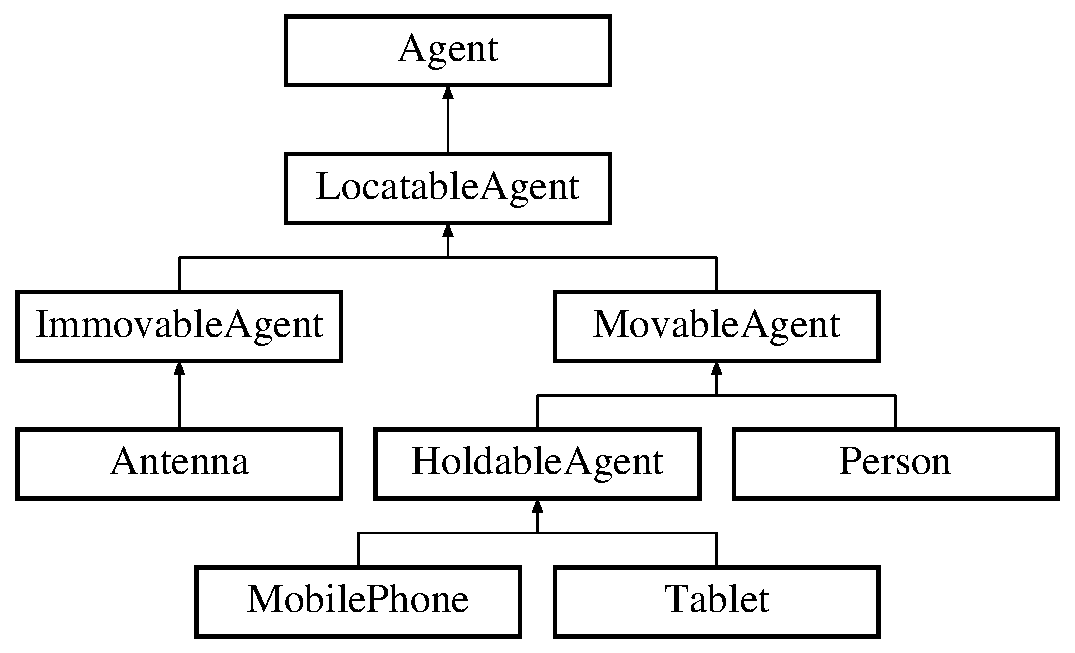
\includegraphics[height=5.000000cm]{class_agent}
\end{center}
\end{figure}
\subsection*{Public Member Functions}
\begin{DoxyCompactItemize}
\item 
\textbf{ Agent} (const \textbf{ Map} $\ast$m, const unsigned long id, const \textbf{ Clock} $\ast$clock)
\item 
virtual \textbf{ $\sim$\+Agent} ()
\item 
bool \textbf{ operator==} (const \textbf{ Agent} \&a)
\item 
virtual const string \textbf{ get\+Name} () const =0
\item 
virtual const string \textbf{ to\+String} () const =0
\item 
const \textbf{ Map} $\ast$ \textbf{ get\+Map} () const
\item 
void \textbf{ set\+Map} (const \textbf{ Map} $\ast$map)
\item 
const \textbf{ Clock} $\ast$ \textbf{ get\+Clock} () const
\item 
const unsigned long \textbf{ get\+Id} () const
\end{DoxyCompactItemize}
\subsection*{Private Attributes}
\begin{DoxyCompactItemize}
\item 
const \textbf{ Map} $\ast$ \textbf{ m\+\_\+map}
\item 
const unsigned long \textbf{ m\+\_\+id}
\item 
const \textbf{ Clock} $\ast$ \textbf{ m\+\_\+clock}
\end{DoxyCompactItemize}


\subsection{Detailed Description}


Definition at line 17 of file Agent.\+h.



\subsection{Constructor \& Destructor Documentation}
\mbox{\label{class_agent_a0ad923f2f9966b65a5d908cb9da4217c}} 
\index{Agent@{Agent}!Agent@{Agent}}
\index{Agent@{Agent}!Agent@{Agent}}
\subsubsection{Agent()}
{\footnotesize\ttfamily Agent\+::\+Agent (\begin{DoxyParamCaption}\item[{const \textbf{ Map} $\ast$}]{m,  }\item[{const unsigned long}]{id,  }\item[{const \textbf{ Clock} $\ast$}]{clock }\end{DoxyParamCaption})}

Constructor of the class. \doxyref{Agent}{p.}{class_agent} is the base class for all agents used in the simulator\+: persons, antennas, devices. \doxyref{Agent}{p.}{class_agent} is an abstract class, the users should build specific subclasses 
\begin{DoxyParams}{Parameters}
{\em m} & -\/ the \doxyref{Map}{p.}{class_map} where the simulation take place. \\
\hline
{\em id} & -\/ the id of this agent, it uniquely identifies the agent \\
\hline
{\em clock} & -\/ the clock used by the simulator, it is the same for all agents \\
\hline
\end{DoxyParams}
\mbox{\label{class_agent_a4feb26df1cf81760a0e411e393c24d4e}} 
\index{Agent@{Agent}!````~Agent@{$\sim$Agent}}
\index{````~Agent@{$\sim$Agent}!Agent@{Agent}}
\subsubsection{$\sim$Agent()}
{\footnotesize\ttfamily virtual Agent\+::$\sim$\+Agent (\begin{DoxyParamCaption}{ }\end{DoxyParamCaption})\hspace{0.3cm}{\ttfamily [virtual]}}

Default destructor of the class. 

\subsection{Member Function Documentation}
\mbox{\label{class_agent_af80a21a067d04788c23d719d07b04038}} 
\index{Agent@{Agent}!getClock@{getClock}}
\index{getClock@{getClock}!Agent@{Agent}}
\subsubsection{getClock()}
{\footnotesize\ttfamily const \textbf{ Clock}$\ast$ Agent\+::get\+Clock (\begin{DoxyParamCaption}{ }\end{DoxyParamCaption}) const}

Returns a pointer to the \doxyref{Clock}{p.}{class_clock} object used for simulation. All Agents use the same \doxyref{Clock}{p.}{class_clock} object for a simulation. \begin{DoxyReturn}{Returns}

\end{DoxyReturn}
\mbox{\label{class_agent_a51d2d781636f524dc151f3da10955613}} 
\index{Agent@{Agent}!getId@{getId}}
\index{getId@{getId}!Agent@{Agent}}
\subsubsection{getId()}
{\footnotesize\ttfamily const unsigned long Agent\+::get\+Id (\begin{DoxyParamCaption}{ }\end{DoxyParamCaption}) const}

Returns the id of the object. \begin{DoxyReturn}{Returns}
the id of the object. 
\end{DoxyReturn}
\mbox{\label{class_agent_ad1870edeea33b059eca75079be2eb002}} 
\index{Agent@{Agent}!getMap@{getMap}}
\index{getMap@{getMap}!Agent@{Agent}}
\subsubsection{getMap()}
{\footnotesize\ttfamily const \textbf{ Map}$\ast$ Agent\+::get\+Map (\begin{DoxyParamCaption}{ }\end{DoxyParamCaption}) const}

Getter that returns a pointer to the map passed to the constructor when the an object was build. \begin{DoxyReturn}{Returns}
a pointer to the \doxyref{Map}{p.}{class_map} object that was passed to the constructor. All agents use the same map for a simulation. 
\end{DoxyReturn}
\mbox{\label{class_agent_afe6c72d91baf9ee4fe77ea1ed7fef3ba}} 
\index{Agent@{Agent}!getName@{getName}}
\index{getName@{getName}!Agent@{Agent}}
\subsubsection{getName()}
{\footnotesize\ttfamily virtual const string Agent\+::get\+Name (\begin{DoxyParamCaption}{ }\end{DoxyParamCaption}) const\hspace{0.3cm}{\ttfamily [pure virtual]}}

This function is used to get the name of the class. It is a pure virtual function, all subclasses implment it and return the actual name of the class. \begin{DoxyReturn}{Returns}
the name of the class. 
\end{DoxyReturn}


Implemented in \textbf{ Holdable\+Agent} \doxyref{}{p.}{class_holdable_agent_ab330bb40de51a957ef8826af629f94a2}, \textbf{ Antenna} \doxyref{}{p.}{class_antenna_a4ad9da1ca9d79f20b331c22b94c57a02}, \textbf{ Person} \doxyref{}{p.}{class_person_aa2a6f8d7f1d94045a03ca578f2ed272c}, \textbf{ Immovable\+Agent} \doxyref{}{p.}{class_immovable_agent_ae8fbccc744f6f806e47dfd242fa67a1c}, \textbf{ Mobile\+Phone} \doxyref{}{p.}{class_mobile_phone_a1eeac3141baafa75ebcf26fc3a0e4068}, \textbf{ Movable\+Agent} \doxyref{}{p.}{class_movable_agent_abcc1218876c39c996f2cb1eba2b96379}, \textbf{ Locatable\+Agent} \doxyref{}{p.}{class_locatable_agent_a754105958bb672744b525538f1584a7b}, and \textbf{ Tablet} \doxyref{}{p.}{class_tablet_adc7196aaee1e9714236b7cd8825d5826}.

\mbox{\label{class_agent_afa2b3a408bb0694aea46fb2bb59bacf7}} 
\index{Agent@{Agent}!operator==@{operator==}}
\index{operator==@{operator==}!Agent@{Agent}}
\subsubsection{operator==()}
{\footnotesize\ttfamily bool Agent\+::operator== (\begin{DoxyParamCaption}\item[{const \textbf{ Agent} \&}]{a }\end{DoxyParamCaption})}

The equal operator for agents. 
\begin{DoxyParams}{Parameters}
{\em a} & the object with which we test the equality \\
\hline
\end{DoxyParams}
\begin{DoxyReturn}{Returns}
true if this object is the equal to a, flase otherwise. Thw objects are considered to be equal if they have the same id. 
\end{DoxyReturn}
\mbox{\label{class_agent_a87a661874cffb03fa9e474e872810260}} 
\index{Agent@{Agent}!setMap@{setMap}}
\index{setMap@{setMap}!Agent@{Agent}}
\subsubsection{setMap()}
{\footnotesize\ttfamily void Agent\+::set\+Map (\begin{DoxyParamCaption}\item[{const \textbf{ Map} $\ast$}]{map }\end{DoxyParamCaption})}

Sets the \doxyref{Map}{p.}{class_map} to be used by this agent during the simulation. It is not advisable to change the map during a simulation. 
\begin{DoxyParams}{Parameters}
{\em map} & pointer to a \doxyref{Map}{p.}{class_map} object. \\
\hline
\end{DoxyParams}
\mbox{\label{class_agent_a44f291596d10c7878b0641d6ec156328}} 
\index{Agent@{Agent}!toString@{toString}}
\index{toString@{toString}!Agent@{Agent}}
\subsubsection{toString()}
{\footnotesize\ttfamily virtual const string Agent\+::to\+String (\begin{DoxyParamCaption}{ }\end{DoxyParamCaption}) const\hspace{0.3cm}{\ttfamily [pure virtual]}}

Builds a string with of the relevant information of the class. It is useful to output on the console or in a file the description of concrete agents. \begin{DoxyReturn}{Returns}
a string representation of the class content. The values of the members are written in this string. 
\end{DoxyReturn}


Implemented in \textbf{ Holdable\+Agent} \doxyref{}{p.}{class_holdable_agent_a2c581226b8994f24b6b2306ae17dbb52}, \textbf{ Antenna} \doxyref{}{p.}{class_antenna_a7fea30e065f49a3cbcee02f60bd033c8}, \textbf{ Person} \doxyref{}{p.}{class_person_a68872538da519d0a04297f43376db27c}, \textbf{ Mobile\+Phone} \doxyref{}{p.}{class_mobile_phone_a2b7e556d12a43e380786ad0eccf3ce04}, \textbf{ Movable\+Agent} \doxyref{}{p.}{class_movable_agent_a1dee2a6bf93f01006fadfb6fba6c9a59}, \textbf{ Locatable\+Agent} \doxyref{}{p.}{class_locatable_agent_a88674f4c8ab9b1b2f3986b226bf4244f}, \textbf{ Immovable\+Agent} \doxyref{}{p.}{class_immovable_agent_a805b0d18035550d902d617a8c7ccc062}, and \textbf{ Tablet} \doxyref{}{p.}{class_tablet_a3fae01e7d526699476221c6a686a4fba}.



\subsection{Member Data Documentation}
\mbox{\label{class_agent_a534f22ebb0573aa1d58d274632e592cf}} 
\index{Agent@{Agent}!m\_clock@{m\_clock}}
\index{m\_clock@{m\_clock}!Agent@{Agent}}
\subsubsection{m\_clock}
{\footnotesize\ttfamily const \textbf{ Clock}$\ast$ Agent\+::m\+\_\+clock\hspace{0.3cm}{\ttfamily [private]}}



Definition at line 80 of file Agent.\+h.

\mbox{\label{class_agent_ad1f52e164c2a829ef4418940567d6e37}} 
\index{Agent@{Agent}!m\_id@{m\_id}}
\index{m\_id@{m\_id}!Agent@{Agent}}
\subsubsection{m\_id}
{\footnotesize\ttfamily const unsigned long Agent\+::m\+\_\+id\hspace{0.3cm}{\ttfamily [private]}}



Definition at line 79 of file Agent.\+h.

\mbox{\label{class_agent_ab24d62bbfc22946d0c72221c8a43f04a}} 
\index{Agent@{Agent}!m\_map@{m\_map}}
\index{m\_map@{m\_map}!Agent@{Agent}}
\subsubsection{m\_map}
{\footnotesize\ttfamily const \textbf{ Map}$\ast$ Agent\+::m\+\_\+map\hspace{0.3cm}{\ttfamily [private]}}



Definition at line 78 of file Agent.\+h.



The documentation for this class was generated from the following file\+:\begin{DoxyCompactItemize}
\item 
include/\textbf{ Agent.\+h}\end{DoxyCompactItemize}

\hypertarget{class_agents_collection}{}\section{Agents\+Collection Class Reference}
\label{class_agents_collection}\index{Agents\+Collection@{Agents\+Collection}}


{\ttfamily \#include $<$Agents\+Collection.\+h$>$}



Collaboration diagram for Agents\+Collection\+:\nopagebreak
\begin{figure}[H]
\begin{center}
\leavevmode
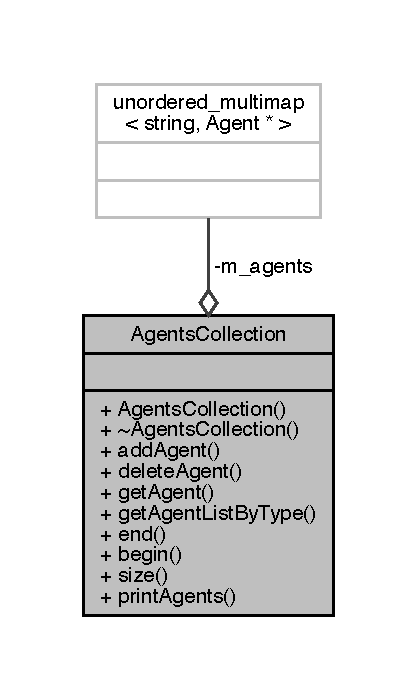
\includegraphics[width=199pt]{class_agents_collection__coll__graph}
\end{center}
\end{figure}
\subsection*{Public Member Functions}
\begin{DoxyCompactItemize}
\item 
\hyperlink{class_agents_collection_a866b0ed56c0109e82bc7c839de0a3267}{Agents\+Collection} ()
\item 
virtual \hyperlink{class_agents_collection_a8a58eb1f8a45cc4d1c0e04dd912dbae0}{$\sim$\+Agents\+Collection} ()
\item 
void \hyperlink{class_agents_collection_a51d14d0635dedd5971ea90dec4f9e7f3}{add\+Agent} (\hyperlink{class_agent}{Agent} $\ast$a)
\item 
\hyperlink{class_agent}{Agent} $\ast$ \hyperlink{class_agents_collection_afd4d2e005b5e449637abd0fa022132a9}{delete\+Agent} (\hyperlink{class_agent}{Agent} $\ast$a)
\item 
\hyperlink{class_agent}{Agent} $\ast$ \hyperlink{class_agents_collection_a4b6b57c50d715edb3404520cfdb32688}{get\+Agent} (const unsigned long id) const
\item 
pair$<$ \hyperlink{_agents_collection_8h_afde47bc45d604b8b8c72755072376679}{um\+\_\+iterator}, \hyperlink{_agents_collection_8h_afde47bc45d604b8b8c72755072376679}{um\+\_\+iterator} $>$ \hyperlink{class_agents_collection_a4ab0c8e86e6f6ebceb12bd2bd8f9f758}{get\+Agent\+List\+By\+Type} (const string \&agent\+Type)
\item 
\hyperlink{_agents_collection_8h_afde47bc45d604b8b8c72755072376679}{um\+\_\+iterator} \hyperlink{class_agents_collection_afc61b751cf3387ab4a1bf0dfbc29cb82}{end} ()
\item 
\hyperlink{_agents_collection_8h_afde47bc45d604b8b8c72755072376679}{um\+\_\+iterator} \hyperlink{class_agents_collection_abc1d6593a3ed1c1c7b2d31b7efec8db8}{begin} ()
\item 
unsigned long \hyperlink{class_agents_collection_a3226f7eb58b11623bdb353d8938f60d3}{size} ()
\item 
void \hyperlink{class_agents_collection_a193faf9793030715e8edeb65137156e9}{print\+Agents} ()
\end{DoxyCompactItemize}
\subsection*{Private Attributes}
\begin{DoxyCompactItemize}
\item 
unordered\+\_\+multimap$<$ string, \hyperlink{class_agent}{Agent} $\ast$ $>$ \hyperlink{class_agents_collection_a35a5728b0e0108c2f37897720c904dd1}{m\+\_\+agents}
\end{DoxyCompactItemize}


\subsection{Detailed Description}
This is actually a container for all the agents used for simulation. An agent could be an object of one the the derived classes of \hyperlink{class_agent}{Agent}. The Agents are kept in an unordered\+\_\+multimap as pairs $<$string, Agent$\ast$$>$ where the first element of the pair is the name of the concrete agent (a person, a mobile device, an antenna, a mno, etc.) and the second element is a pointer to the actual object (agent). 

\subsection{Constructor \& Destructor Documentation}
\mbox{\Hypertarget{class_agents_collection_a866b0ed56c0109e82bc7c839de0a3267}\label{class_agents_collection_a866b0ed56c0109e82bc7c839de0a3267}} 
\index{Agents\+Collection@{Agents\+Collection}!Agents\+Collection@{Agents\+Collection}}
\index{Agents\+Collection@{Agents\+Collection}!Agents\+Collection@{Agents\+Collection}}
\subsubsection{\texorpdfstring{Agents\+Collection()}{AgentsCollection()}}
{\footnotesize\ttfamily Agents\+Collection\+::\+Agents\+Collection (\begin{DoxyParamCaption}{ }\end{DoxyParamCaption})}

The default constructor of the class. \mbox{\Hypertarget{class_agents_collection_a8a58eb1f8a45cc4d1c0e04dd912dbae0}\label{class_agents_collection_a8a58eb1f8a45cc4d1c0e04dd912dbae0}} 
\index{Agents\+Collection@{Agents\+Collection}!````~Agents\+Collection@{$\sim$\+Agents\+Collection}}
\index{````~Agents\+Collection@{$\sim$\+Agents\+Collection}!Agents\+Collection@{Agents\+Collection}}
\subsubsection{\texorpdfstring{$\sim$\+Agents\+Collection()}{~AgentsCollection()}}
{\footnotesize\ttfamily virtual Agents\+Collection\+::$\sim$\+Agents\+Collection (\begin{DoxyParamCaption}{ }\end{DoxyParamCaption})\hspace{0.3cm}{\ttfamily [virtual]}}

Default destructor\+: it iterates through the collection of agents and frees the memory allocated for each agent in the collection. 

\subsection{Member Function Documentation}
\mbox{\Hypertarget{class_agents_collection_a51d14d0635dedd5971ea90dec4f9e7f3}\label{class_agents_collection_a51d14d0635dedd5971ea90dec4f9e7f3}} 
\index{Agents\+Collection@{Agents\+Collection}!add\+Agent@{add\+Agent}}
\index{add\+Agent@{add\+Agent}!Agents\+Collection@{Agents\+Collection}}
\subsubsection{\texorpdfstring{add\+Agent()}{addAgent()}}
{\footnotesize\ttfamily void Agents\+Collection\+::add\+Agent (\begin{DoxyParamCaption}\item[{\hyperlink{class_agent}{Agent} $\ast$}]{a }\end{DoxyParamCaption})}

Adds a new \hyperlink{class_agent}{Agent} to the collection. For performance reasons the \hyperlink{class_agents_collection}{Agents\+Collection} class keep only a pointer to actual agents (objects). 
\begin{DoxyParams}{Parameters}
{\em a} & a pointer to the object (one of the derived classes of the \hyperlink{class_agent}{Agent}) to be added to the collection. \\
\hline
\end{DoxyParams}
\mbox{\Hypertarget{class_agents_collection_abc1d6593a3ed1c1c7b2d31b7efec8db8}\label{class_agents_collection_abc1d6593a3ed1c1c7b2d31b7efec8db8}} 
\index{Agents\+Collection@{Agents\+Collection}!begin@{begin}}
\index{begin@{begin}!Agents\+Collection@{Agents\+Collection}}
\subsubsection{\texorpdfstring{begin()}{begin()}}
{\footnotesize\ttfamily \hyperlink{_agents_collection_8h_afde47bc45d604b8b8c72755072376679}{um\+\_\+iterator} Agents\+Collection\+::begin (\begin{DoxyParamCaption}{ }\end{DoxyParamCaption})}

Iterator to the first agent of the container. \begin{DoxyReturn}{Returns}
a random access iterator pointing to the first element (agent) in the container. If the container is empty, the returned iterator value shall not be dereferenced. 
\end{DoxyReturn}
\mbox{\Hypertarget{class_agents_collection_afd4d2e005b5e449637abd0fa022132a9}\label{class_agents_collection_afd4d2e005b5e449637abd0fa022132a9}} 
\index{Agents\+Collection@{Agents\+Collection}!delete\+Agent@{delete\+Agent}}
\index{delete\+Agent@{delete\+Agent}!Agents\+Collection@{Agents\+Collection}}
\subsubsection{\texorpdfstring{delete\+Agent()}{deleteAgent()}}
{\footnotesize\ttfamily \hyperlink{class_agent}{Agent}$\ast$ Agents\+Collection\+::delete\+Agent (\begin{DoxyParamCaption}\item[{\hyperlink{class_agent}{Agent} $\ast$}]{a }\end{DoxyParamCaption})}

Removes an object from the collection. 
\begin{DoxyParams}{Parameters}
{\em a} & a pointer to the object to be removed from the collection. \\
\hline
\end{DoxyParams}
\begin{DoxyReturn}{Returns}

\end{DoxyReturn}
\mbox{\Hypertarget{class_agents_collection_afc61b751cf3387ab4a1bf0dfbc29cb82}\label{class_agents_collection_afc61b751cf3387ab4a1bf0dfbc29cb82}} 
\index{Agents\+Collection@{Agents\+Collection}!end@{end}}
\index{end@{end}!Agents\+Collection@{Agents\+Collection}}
\subsubsection{\texorpdfstring{end()}{end()}}
{\footnotesize\ttfamily \hyperlink{_agents_collection_8h_afde47bc45d604b8b8c72755072376679}{um\+\_\+iterator} Agents\+Collection\+::end (\begin{DoxyParamCaption}{ }\end{DoxyParamCaption})}

Iterator to the past-\/the-\/end of the collection. It does not point to any agent, and thus shall not be dereferenced. \begin{DoxyReturn}{Returns}
an iterator referring to the past-\/the-\/end element in the agents container. If the container is empty, this function returns the same as Agents\+Colletion\+::begin(). 
\end{DoxyReturn}
\mbox{\Hypertarget{class_agents_collection_a4b6b57c50d715edb3404520cfdb32688}\label{class_agents_collection_a4b6b57c50d715edb3404520cfdb32688}} 
\index{Agents\+Collection@{Agents\+Collection}!get\+Agent@{get\+Agent}}
\index{get\+Agent@{get\+Agent}!Agents\+Collection@{Agents\+Collection}}
\subsubsection{\texorpdfstring{get\+Agent()}{getAgent()}}
{\footnotesize\ttfamily \hyperlink{class_agent}{Agent}$\ast$ Agents\+Collection\+::get\+Agent (\begin{DoxyParamCaption}\item[{const unsigned long}]{id }\end{DoxyParamCaption}) const}

Returns a pointer to an agent from the collection. The agent/object is identified by its id. 
\begin{DoxyParams}{Parameters}
{\em id} & the id of the agent to be returned. \\
\hline
\end{DoxyParams}
\begin{DoxyReturn}{Returns}
a pointer to the agent with the id equal to the parameter id. If there is no agent with the provided id, this method returns nullptr. 
\end{DoxyReturn}
\mbox{\Hypertarget{class_agents_collection_a4ab0c8e86e6f6ebceb12bd2bd8f9f758}\label{class_agents_collection_a4ab0c8e86e6f6ebceb12bd2bd8f9f758}} 
\index{Agents\+Collection@{Agents\+Collection}!get\+Agent\+List\+By\+Type@{get\+Agent\+List\+By\+Type}}
\index{get\+Agent\+List\+By\+Type@{get\+Agent\+List\+By\+Type}!Agents\+Collection@{Agents\+Collection}}
\subsubsection{\texorpdfstring{get\+Agent\+List\+By\+Type()}{getAgentListByType()}}
{\footnotesize\ttfamily pair$<$\hyperlink{_agents_collection_8h_afde47bc45d604b8b8c72755072376679}{um\+\_\+iterator}, \hyperlink{_agents_collection_8h_afde47bc45d604b8b8c72755072376679}{um\+\_\+iterator}$>$ Agents\+Collection\+::get\+Agent\+List\+By\+Type (\begin{DoxyParamCaption}\item[{const string \&}]{agent\+Type }\end{DoxyParamCaption})}

This method is used to get a subset with a certain type of agents\+: persons, mobile phones etc. 
\begin{DoxyParams}{Parameters}
{\em agent\+Type} & is the name of the class of agents that the user wants to retrieve from the collection of all agents. \\
\hline
\end{DoxyParams}
\begin{DoxyReturn}{Returns}
a std\+::pair of iterators of type unordered\+\_\+multimap$<$string, Agent$\ast$$>$\+::iterator that can be used to iterate through to subset of the agents. 
\end{DoxyReturn}
\mbox{\Hypertarget{class_agents_collection_a193faf9793030715e8edeb65137156e9}\label{class_agents_collection_a193faf9793030715e8edeb65137156e9}} 
\index{Agents\+Collection@{Agents\+Collection}!print\+Agents@{print\+Agents}}
\index{print\+Agents@{print\+Agents}!Agents\+Collection@{Agents\+Collection}}
\subsubsection{\texorpdfstring{print\+Agents()}{printAgents()}}
{\footnotesize\ttfamily void Agents\+Collection\+::print\+Agents (\begin{DoxyParamCaption}{ }\end{DoxyParamCaption})}

Print out all agents in the collection. \mbox{\Hypertarget{class_agents_collection_a3226f7eb58b11623bdb353d8938f60d3}\label{class_agents_collection_a3226f7eb58b11623bdb353d8938f60d3}} 
\index{Agents\+Collection@{Agents\+Collection}!size@{size}}
\index{size@{size}!Agents\+Collection@{Agents\+Collection}}
\subsubsection{\texorpdfstring{size()}{size()}}
{\footnotesize\ttfamily unsigned long Agents\+Collection\+::size (\begin{DoxyParamCaption}{ }\end{DoxyParamCaption})}

\begin{DoxyReturn}{Returns}
the number of elements in the container. This is the number of actual objects held in the container, which is not necessarily equal to its storage capacity. 
\end{DoxyReturn}


\subsection{Member Data Documentation}
\mbox{\Hypertarget{class_agents_collection_a35a5728b0e0108c2f37897720c904dd1}\label{class_agents_collection_a35a5728b0e0108c2f37897720c904dd1}} 
\index{Agents\+Collection@{Agents\+Collection}!m\+\_\+agents@{m\+\_\+agents}}
\index{m\+\_\+agents@{m\+\_\+agents}!Agents\+Collection@{Agents\+Collection}}
\subsubsection{\texorpdfstring{m\+\_\+agents}{m\_agents}}
{\footnotesize\ttfamily unordered\+\_\+multimap$<$string, \hyperlink{class_agent}{Agent}$\ast$$>$ Agents\+Collection\+::m\+\_\+agents\hspace{0.3cm}{\ttfamily [private]}}



The documentation for this class was generated from the following file\+:\begin{DoxyCompactItemize}
\item 
include/agent/\hyperlink{_agents_collection_8h}{Agents\+Collection.\+h}\end{DoxyCompactItemize}

\section{Antenna Class Reference}
\label{class_antenna}\index{Antenna@{Antenna}}


{\ttfamily \#include $<$Antenna.\+h$>$}

Inheritance diagram for Antenna\+:\begin{figure}[H]
\begin{center}
\leavevmode
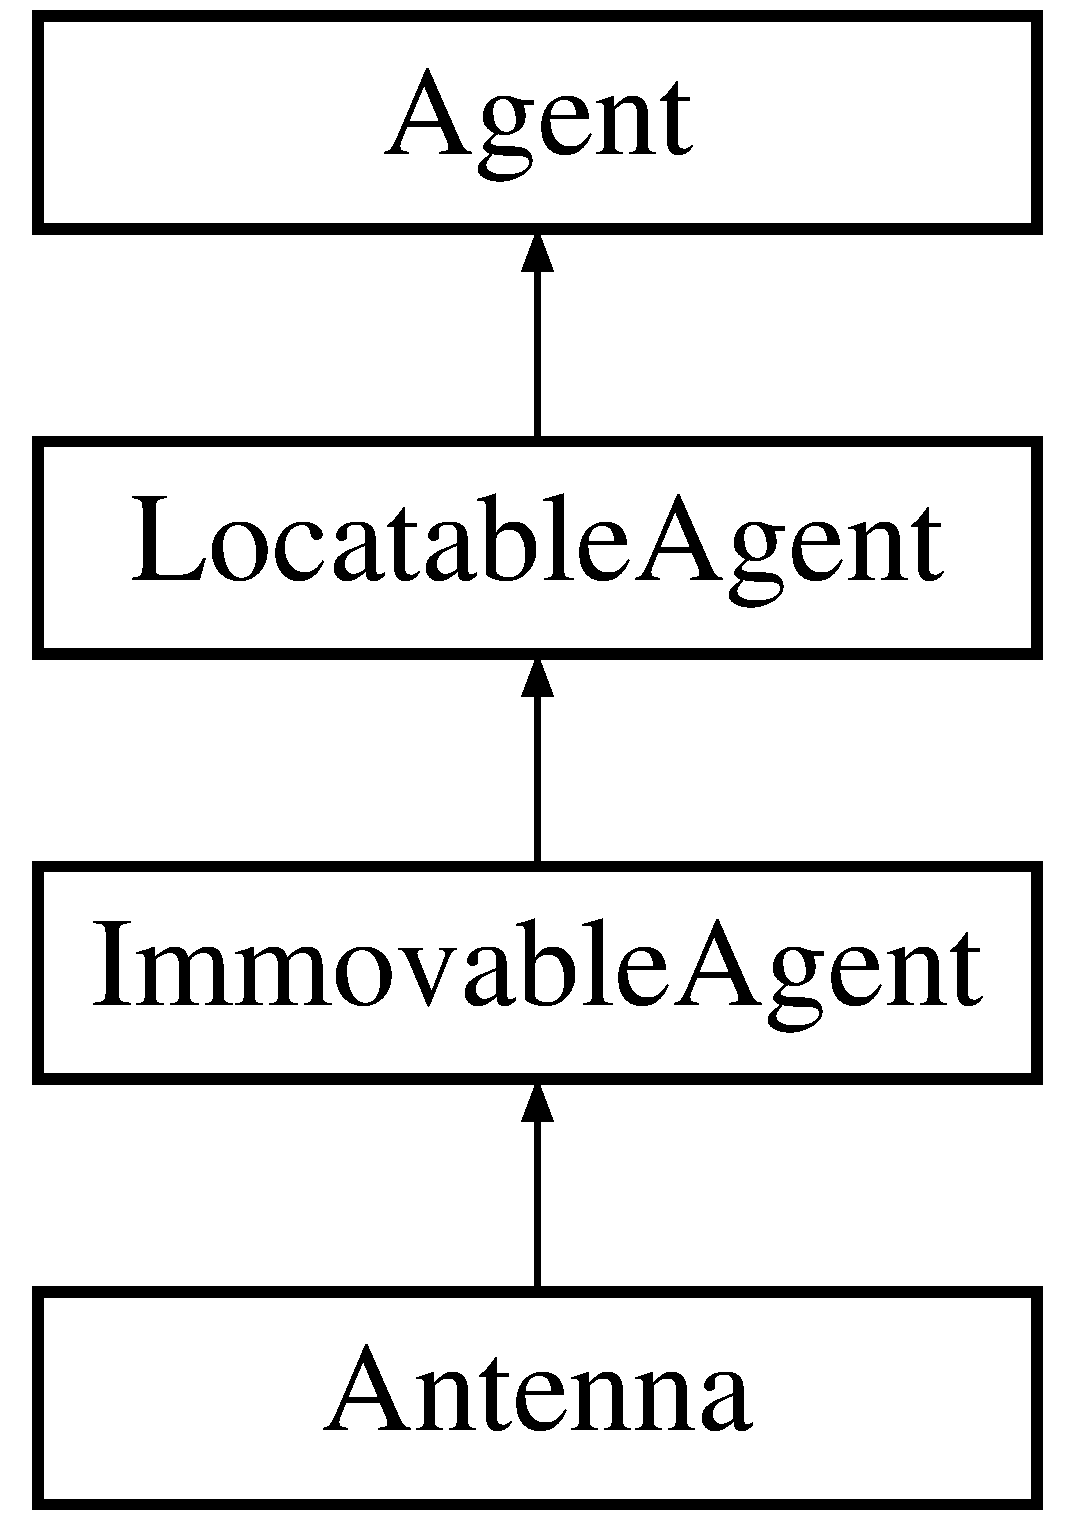
\includegraphics[height=4.000000cm]{class_antenna}
\end{center}
\end{figure}
\subsection*{Public Member Functions}
\begin{DoxyCompactItemize}
\item 
\textbf{ Antenna} (const \textbf{ Map} $\ast$m, const unsigned long id, Point $\ast$init\+Position, const \textbf{ Clock} $\ast$clock, double attenuation\+Factor, double power, unsigned long max\+Connections, double smid, double ssteep, \textbf{ Antenna\+Type} type)
\item 
\textbf{ Antenna} (const \textbf{ Map} $\ast$m, const \textbf{ Clock} $\ast$clock, const unsigned long id, X\+M\+L\+Element $\ast$el)
\item 
virtual \textbf{ $\sim$\+Antenna} ()
\item 
const string \textbf{ get\+Name} () const override
\item 
const string \textbf{ to\+String} () const override
\item 
double \textbf{ get\+Attenuation\+Factor} () const
\item 
void \textbf{ set\+Attenuation\+Factor} (double attenuation\+Factor)
\item 
double \textbf{ get\+Power} () const
\item 
void \textbf{ set\+Power} (double power)
\item 
unsigned long \textbf{ get\+Max\+Connections} () const
\item 
void \textbf{ set\+Max\+Connections} (int max\+Connections)
\item 
bool \textbf{ try\+Register\+Device} (\textbf{ Holdable\+Agent} $\ast$device)
\item 
void \textbf{ attach\+Device} (\textbf{ Holdable\+Agent} $\ast$device)
\item 
void \textbf{ dettach\+Device} (\textbf{ Holdable\+Agent} $\ast$device)
\item 
\textbf{ Antenna\+Type} \textbf{ get\+Type} () const
\item 
void \textbf{ set\+Type} (\textbf{ Antenna\+Type} type)
\item 
double \textbf{ S} (double dist) const
\item 
double \textbf{ get\+Smid} () const
\item 
void \textbf{ set\+Smid} (double smid)
\item 
double \textbf{ get\+S\+Steep} () const
\item 
void \textbf{ set\+S\+Steep} (double s\+Steep)
\item 
double \textbf{ compute\+Signal\+Quality} (const Point $\ast$p) const
\item 
double \textbf{ compute\+Power} (const Point $\ast$p) const
\end{DoxyCompactItemize}
\subsection*{Private Member Functions}
\begin{DoxyCompactItemize}
\item 
bool \textbf{ already\+Registered} (\textbf{ Holdable\+Agent} $\ast$ag)
\item 
void \textbf{ register\+Event} (\textbf{ Holdable\+Agent} $\ast$ag, const \textbf{ Event\+Type} event, const bool verbose)
\item 
unsigned long \textbf{ get\+Num\+Active\+Conections} ()
\item 
double \textbf{ S0} () const
\item 
double \textbf{ S\+Dist} (double dist) const
\end{DoxyCompactItemize}
\subsection*{Private Attributes}
\begin{DoxyCompactItemize}
\item 
double \textbf{ m\+\_\+attenuation\+Factor}
\item 
double \textbf{ m\+\_\+power}
\item 
unsigned long \textbf{ m\+\_\+max\+Connections}
\item 
double \textbf{ m\+\_\+\+Smid}
\item 
double \textbf{ m\+\_\+\+S\+Steep}
\item 
Polygon $\ast$ \textbf{ m\+\_\+cell}
\item 
vector$<$ \textbf{ Holdable\+Agent} $\ast$ $>$ \textbf{ m\+\_\+devices}
\item 
\textbf{ Antenna\+Type} \textbf{ m\+\_\+type}
\item 
ofstream \textbf{ m\+\_\+file}
\end{DoxyCompactItemize}


\subsection{Detailed Description}
This class simulates an antenna of the mobile phone network. 

Definition at line 29 of file Antenna.\+h.



\subsection{Constructor \& Destructor Documentation}
\mbox{\label{class_antenna_a39c505109145908a5b032a16a2fe53c4}} 
\index{Antenna@{Antenna}!Antenna@{Antenna}}
\index{Antenna@{Antenna}!Antenna@{Antenna}}
\subsubsection{Antenna()\hspace{0.1cm}{\footnotesize\ttfamily [1/2]}}
{\footnotesize\ttfamily Antenna\+::\+Antenna (\begin{DoxyParamCaption}\item[{const \textbf{ Map} $\ast$}]{m,  }\item[{const unsigned long}]{id,  }\item[{Point $\ast$}]{init\+Position,  }\item[{const \textbf{ Clock} $\ast$}]{clock,  }\item[{double}]{attenuation\+Factor,  }\item[{double}]{power,  }\item[{unsigned long}]{max\+Connections,  }\item[{double}]{smid,  }\item[{double}]{ssteep,  }\item[{\textbf{ Antenna\+Type}}]{type }\end{DoxyParamCaption})\hspace{0.3cm}{\ttfamily [explicit]}}

Constructor of the class. It builds an object providing directly the values for each parameter of the antenna. 
\begin{DoxyParams}{Parameters}
{\em m} & a pointer to the \doxyref{Map}{p.}{class_map} object used for the simulation \\
\hline
{\em id} & the id of the \doxyref{Antenna}{p.}{class_antenna} \\
\hline
{\em init\+Position} & the position of the antenna on the map \\
\hline
{\em clock} & a pointer to the \doxyref{Clock}{p.}{class_clock} object used for the simulation \\
\hline
{\em attenuation\+Factor} & the attenuation factor of the surrounding environment. In real life, it takes values between 2 (in open field) and 6 (inside buildings). \\
\hline
{\em power} & the power of the antenna in Watts. \\
\hline
{\em max\+Connections} & the maximum number of the connections that the antenna can accept. \\
\hline
{\em smid} & is a parameter of an antenna. The significance of this parameter is described in mobloc R package. \\
\hline
{\em ssteep} & is a parameter of an antenna. The significance of this parameter is described in mobloc R package. \\
\hline
{\em type} & it could have two values \doxyref{Antenna\+Type\+::\+O\+M\+N\+I\+D\+I\+R\+E\+C\+T\+I\+O\+N\+AL}{p.}{_antenna_type_8h_a7b678b5cb9dedc607131200119d96b16a8ff57fa72952e98025e600a041b8b8de} for omnidirectional antennas and \doxyref{Antenna\+Type\+::\+D\+I\+R\+E\+C\+T\+I\+O\+N\+AL}{p.}{_antenna_type_8h_a7b678b5cb9dedc607131200119d96b16ab6f2249394a4def60a78b342dcc925b9} for directional antennas. \\
\hline
\end{DoxyParams}
\mbox{\label{class_antenna_a86c73cfb78910fbaedd6ceb4e226dc9b}} 
\index{Antenna@{Antenna}!Antenna@{Antenna}}
\index{Antenna@{Antenna}!Antenna@{Antenna}}
\subsubsection{Antenna()\hspace{0.1cm}{\footnotesize\ttfamily [2/2]}}
{\footnotesize\ttfamily Antenna\+::\+Antenna (\begin{DoxyParamCaption}\item[{const \textbf{ Map} $\ast$}]{m,  }\item[{const \textbf{ Clock} $\ast$}]{clock,  }\item[{const unsigned long}]{id,  }\item[{X\+M\+L\+Element $\ast$}]{el }\end{DoxyParamCaption})\hspace{0.3cm}{\ttfamily [explicit]}}

Constructor of the class. It builds an object taking the value of the antenna\textquotesingle{} parameters from an X\+ML Element, usually when an \doxyref{Antenna}{p.}{class_antenna} object is built reading the xml configuration file. 
\begin{DoxyParams}{Parameters}
{\em m} & a pointer to the \doxyref{Map}{p.}{class_map} object used for the simulation \\
\hline
{\em clock} & a pointer to the \doxyref{Clock}{p.}{class_clock} object used for the simulation \\
\hline
{\em id} & the id of the \doxyref{Antenna}{p.}{class_antenna} \\
\hline
{\em el} & the X\+ML Element containing the parameters of the \doxyref{Antenna}{p.}{class_antenna}. \\
\hline
\end{DoxyParams}
\mbox{\label{class_antenna_ad7b98073b970db5d6bc83c5c5961fe44}} 
\index{Antenna@{Antenna}!````~Antenna@{$\sim$Antenna}}
\index{````~Antenna@{$\sim$Antenna}!Antenna@{Antenna}}
\subsubsection{$\sim$Antenna()}
{\footnotesize\ttfamily virtual Antenna\+::$\sim$\+Antenna (\begin{DoxyParamCaption}{ }\end{DoxyParamCaption})\hspace{0.3cm}{\ttfamily [virtual]}}

Destructor of the class. It closes the file where the \doxyref{Antenna}{p.}{class_antenna} dumps the registered events during the simulation. 

\subsection{Member Function Documentation}
\mbox{\label{class_antenna_af4fb83843393bf36bdcaefae5b5dd0dd}} 
\index{Antenna@{Antenna}!alreadyRegistered@{alreadyRegistered}}
\index{alreadyRegistered@{alreadyRegistered}!Antenna@{Antenna}}
\subsubsection{alreadyRegistered()}
{\footnotesize\ttfamily bool Antenna\+::already\+Registered (\begin{DoxyParamCaption}\item[{\textbf{ Holdable\+Agent} $\ast$}]{ag }\end{DoxyParamCaption})\hspace{0.3cm}{\ttfamily [private]}}

\mbox{\label{class_antenna_a9c804d991a545157feb066761b6a69ef}} 
\index{Antenna@{Antenna}!attachDevice@{attachDevice}}
\index{attachDevice@{attachDevice}!Antenna@{Antenna}}
\subsubsection{attachDevice()}
{\footnotesize\ttfamily void Antenna\+::attach\+Device (\begin{DoxyParamCaption}\item[{\textbf{ Holdable\+Agent} $\ast$}]{device }\end{DoxyParamCaption})}

Connects a new mobile device and outputs an event \doxyref{Event\+Type\+::\+A\+T\+T\+A\+C\+H\+\_\+\+D\+E\+V\+I\+CE}{p.}{_event_type_8h_a2628ea8d12e8b2563c32f05dc7fff6faa9893a3a649e7100d87b1560bd8202ec2} in the output file. Internally, the antenna keeps a vector with all connected mobile devices. devices. When a new mobile device is connected it is added to this vector. 
\begin{DoxyParams}{Parameters}
{\em device} & a pointer to the object that represents the mobile device connected to this antenna. \\
\hline
\end{DoxyParams}
\mbox{\label{class_antenna_a7caa8004be14f97db64fdf7ae46d6c97}} 
\index{Antenna@{Antenna}!computePower@{computePower}}
\index{computePower@{computePower}!Antenna@{Antenna}}
\subsubsection{computePower()}
{\footnotesize\ttfamily double Antenna\+::compute\+Power (\begin{DoxyParamCaption}\item[{const Point $\ast$}]{p }\end{DoxyParamCaption}) const}

Computes the power of the signal given by an antenna in a certain location. 
\begin{DoxyParams}{Parameters}
{\em p} & the location where we want to compute the power of the signal. \\
\hline
\end{DoxyParams}
\begin{DoxyReturn}{Returns}
the power of the signal in the location given by Point p. 
\end{DoxyReturn}
\mbox{\label{class_antenna_afb03d417efec2423a1b67df16d6ebcb6}} 
\index{Antenna@{Antenna}!computeSignalQuality@{computeSignalQuality}}
\index{computeSignalQuality@{computeSignalQuality}!Antenna@{Antenna}}
\subsubsection{computeSignalQuality()}
{\footnotesize\ttfamily double Antenna\+::compute\+Signal\+Quality (\begin{DoxyParamCaption}\item[{const Point $\ast$}]{p }\end{DoxyParamCaption}) const}

Computes the signal quality given by an antenna in a certain location. 
\begin{DoxyParams}{Parameters}
{\em p} & the location where we want to compute the signal quality. \\
\hline
\end{DoxyParams}
\begin{DoxyReturn}{Returns}
the signal quality. 
\end{DoxyReturn}
\mbox{\label{class_antenna_a983a0784315567c2ab6ac1820cf558c5}} 
\index{Antenna@{Antenna}!dettachDevice@{dettachDevice}}
\index{dettachDevice@{dettachDevice}!Antenna@{Antenna}}
\subsubsection{dettachDevice()}
{\footnotesize\ttfamily void Antenna\+::dettach\+Device (\begin{DoxyParamCaption}\item[{\textbf{ Holdable\+Agent} $\ast$}]{device }\end{DoxyParamCaption})}

Disconnects a mobile device from the antenna and outputs an event Event\+Type\+::\+D\+E\+A\+T\+A\+C\+H\+\_\+\+D\+E\+V\+I\+CE in the output file. Internally, the mobile device is removed from the vector of the connected mobile devices. 
\begin{DoxyParams}{Parameters}
{\em device} & \\
\hline
\end{DoxyParams}
\mbox{\label{class_antenna_a9551ed22d25c51210913de4a3074d9eb}} 
\index{Antenna@{Antenna}!getAttenuationFactor@{getAttenuationFactor}}
\index{getAttenuationFactor@{getAttenuationFactor}!Antenna@{Antenna}}
\subsubsection{getAttenuationFactor()}
{\footnotesize\ttfamily double Antenna\+::get\+Attenuation\+Factor (\begin{DoxyParamCaption}{ }\end{DoxyParamCaption}) const}

Returns the surrounding environment\textquotesingle{} attenuation factor of the signal. \begin{DoxyReturn}{Returns}
the signals\textquotesingle{} attenuation factor of the surrounding environment. In real life, it takes values between 2 (in open field) and 6 (inside buildings). 
\end{DoxyReturn}
\mbox{\label{class_antenna_ac7d42215283cd7d4dc16d449f61af91d}} 
\index{Antenna@{Antenna}!getMaxConnections@{getMaxConnections}}
\index{getMaxConnections@{getMaxConnections}!Antenna@{Antenna}}
\subsubsection{getMaxConnections()}
{\footnotesize\ttfamily unsigned long Antenna\+::get\+Max\+Connections (\begin{DoxyParamCaption}{ }\end{DoxyParamCaption}) const}

Returns the maximum number of mobile devices that an antenna can connect. \mbox{\label{class_antenna_a4ad9da1ca9d79f20b331c22b94c57a02}} 
\index{Antenna@{Antenna}!getName@{getName}}
\index{getName@{getName}!Antenna@{Antenna}}
\subsubsection{getName()}
{\footnotesize\ttfamily const string Antenna\+::get\+Name (\begin{DoxyParamCaption}{ }\end{DoxyParamCaption}) const\hspace{0.3cm}{\ttfamily [override]}, {\ttfamily [virtual]}}

Overrides the same method from the superclass. \begin{DoxyReturn}{Returns}
the name of the class, i.\+e. \char`\"{}\+Antenna\char`\"{} 
\end{DoxyReturn}


Implements \textbf{ Agent} \doxyref{}{p.}{class_agent_afe6c72d91baf9ee4fe77ea1ed7fef3ba}.

\mbox{\label{class_antenna_a86c5c094ab6ea432609afa00f3a8080a}} 
\index{Antenna@{Antenna}!getNumActiveConections@{getNumActiveConections}}
\index{getNumActiveConections@{getNumActiveConections}!Antenna@{Antenna}}
\subsubsection{getNumActiveConections()}
{\footnotesize\ttfamily unsigned long Antenna\+::get\+Num\+Active\+Conections (\begin{DoxyParamCaption}{ }\end{DoxyParamCaption})\hspace{0.3cm}{\ttfamily [private]}}

\mbox{\label{class_antenna_afca01d00c8e393ee911f1e9240b51d2e}} 
\index{Antenna@{Antenna}!getPower@{getPower}}
\index{getPower@{getPower}!Antenna@{Antenna}}
\subsubsection{getPower()}
{\footnotesize\ttfamily double Antenna\+::get\+Power (\begin{DoxyParamCaption}{ }\end{DoxyParamCaption}) const}

Returns the power of an antenna in Watts at the location of antenna. This power decreases with a power of the distance from antenna. \begin{DoxyReturn}{Returns}
the power of an antenna in Watts. 
\end{DoxyReturn}
\mbox{\label{class_antenna_acfaf47d35cc742e76522ea31a8b01578}} 
\index{Antenna@{Antenna}!getSmid@{getSmid}}
\index{getSmid@{getSmid}!Antenna@{Antenna}}
\subsubsection{getSmid()}
{\footnotesize\ttfamily double Antenna\+::get\+Smid (\begin{DoxyParamCaption}{ }\end{DoxyParamCaption}) const}

Returns the value of the Smid antenna parameter. \begin{DoxyReturn}{Returns}
the value of the Smid antenna parameter. 
\end{DoxyReturn}
\mbox{\label{class_antenna_a096deca0fe8497c0fe53539ae80f2db5}} 
\index{Antenna@{Antenna}!getSSteep@{getSSteep}}
\index{getSSteep@{getSSteep}!Antenna@{Antenna}}
\subsubsection{getSSteep()}
{\footnotesize\ttfamily double Antenna\+::get\+S\+Steep (\begin{DoxyParamCaption}{ }\end{DoxyParamCaption}) const}

Returns the value of the Ssteep antenna parameter. \begin{DoxyReturn}{Returns}
the value of the Ssteep antenna parameter. 
\end{DoxyReturn}
\mbox{\label{class_antenna_adf45a8b339956741bf8dcb5361f5f249}} 
\index{Antenna@{Antenna}!getType@{getType}}
\index{getType@{getType}!Antenna@{Antenna}}
\subsubsection{getType()}
{\footnotesize\ttfamily \textbf{ Antenna\+Type} Antenna\+::get\+Type (\begin{DoxyParamCaption}{ }\end{DoxyParamCaption}) const}

Returns the antenna type\+: omnidirectional or directional \begin{DoxyReturn}{Returns}
the antenna type \+: \doxyref{Antenna\+Type\+::\+O\+M\+N\+I\+D\+I\+R\+E\+C\+T\+I\+O\+N\+AL}{p.}{_antenna_type_8h_a7b678b5cb9dedc607131200119d96b16a8ff57fa72952e98025e600a041b8b8de} or \doxyref{Antenna\+Type\+::\+D\+I\+R\+E\+C\+T\+I\+O\+N\+AL}{p.}{_antenna_type_8h_a7b678b5cb9dedc607131200119d96b16ab6f2249394a4def60a78b342dcc925b9}. 
\end{DoxyReturn}
\mbox{\label{class_antenna_aa21a4c0d581c59c36480d932584c0ef5}} 
\index{Antenna@{Antenna}!registerEvent@{registerEvent}}
\index{registerEvent@{registerEvent}!Antenna@{Antenna}}
\subsubsection{registerEvent()}
{\footnotesize\ttfamily void Antenna\+::register\+Event (\begin{DoxyParamCaption}\item[{\textbf{ Holdable\+Agent} $\ast$}]{ag,  }\item[{const \textbf{ Event\+Type}}]{event,  }\item[{const bool}]{verbose }\end{DoxyParamCaption})\hspace{0.3cm}{\ttfamily [private]}}

\mbox{\label{class_antenna_a5715c4100035c58d63b7c9a0195748fe}} 
\index{Antenna@{Antenna}!S@{S}}
\index{S@{S}!Antenna@{Antenna}}
\subsubsection{S()}
{\footnotesize\ttfamily double Antenna\+::S (\begin{DoxyParamCaption}\item[{double}]{dist }\end{DoxyParamCaption}) const}

Computes the signal strength at the distance dist from antenna location. 
\begin{DoxyParams}{Parameters}
{\em dist} & the distance from antenna location. \\
\hline
\end{DoxyParams}
\begin{DoxyReturn}{Returns}
the signal strength. 
\end{DoxyReturn}
\mbox{\label{class_antenna_a033246c50bec80123860154a949620c7}} 
\index{Antenna@{Antenna}!S0@{S0}}
\index{S0@{S0}!Antenna@{Antenna}}
\subsubsection{S0()}
{\footnotesize\ttfamily double Antenna\+::\+S0 (\begin{DoxyParamCaption}{ }\end{DoxyParamCaption}) const\hspace{0.3cm}{\ttfamily [private]}}

\mbox{\label{class_antenna_ae60ab40ded94be407c3b7455f4e886fe}} 
\index{Antenna@{Antenna}!SDist@{SDist}}
\index{SDist@{SDist}!Antenna@{Antenna}}
\subsubsection{SDist()}
{\footnotesize\ttfamily double Antenna\+::\+S\+Dist (\begin{DoxyParamCaption}\item[{double}]{dist }\end{DoxyParamCaption}) const\hspace{0.3cm}{\ttfamily [private]}}

\mbox{\label{class_antenna_a8697756860ff821a92e9404e00a55f89}} 
\index{Antenna@{Antenna}!setAttenuationFactor@{setAttenuationFactor}}
\index{setAttenuationFactor@{setAttenuationFactor}!Antenna@{Antenna}}
\subsubsection{setAttenuationFactor()}
{\footnotesize\ttfamily void Antenna\+::set\+Attenuation\+Factor (\begin{DoxyParamCaption}\item[{double}]{attenuation\+Factor }\end{DoxyParamCaption})}

Sets the surrounding environment\textquotesingle{} attenuation factor of the signal for an antenna. 
\begin{DoxyParams}{Parameters}
{\em attenuation\+Factor} & the value of the surrounding environment\textquotesingle{} attenuation factor of the signal. In real life, it takes values between 2 (in open field) and 6 (inside buildings). \\
\hline
\end{DoxyParams}
\mbox{\label{class_antenna_ad844ed8507afb83b74b804c2434a4e50}} 
\index{Antenna@{Antenna}!setMaxConnections@{setMaxConnections}}
\index{setMaxConnections@{setMaxConnections}!Antenna@{Antenna}}
\subsubsection{setMaxConnections()}
{\footnotesize\ttfamily void Antenna\+::set\+Max\+Connections (\begin{DoxyParamCaption}\item[{int}]{max\+Connections }\end{DoxyParamCaption})}

Sets the number of mobile devices that an antenna can connect. 
\begin{DoxyParams}{Parameters}
{\em max\+Connections} & the number of mobile devices that an antenna can connect. \\
\hline
\end{DoxyParams}
\mbox{\label{class_antenna_a172a4c7765dea045d6504f6e2cbe0f59}} 
\index{Antenna@{Antenna}!setPower@{setPower}}
\index{setPower@{setPower}!Antenna@{Antenna}}
\subsubsection{setPower()}
{\footnotesize\ttfamily void Antenna\+::set\+Power (\begin{DoxyParamCaption}\item[{double}]{power }\end{DoxyParamCaption})}

Sets the power of an antenna. 
\begin{DoxyParams}{Parameters}
{\em power} & the value of the antenna\textquotesingle{}s power. \\
\hline
\end{DoxyParams}
\mbox{\label{class_antenna_a67e5ae0106189d18e4f114d8e0e14a09}} 
\index{Antenna@{Antenna}!setSmid@{setSmid}}
\index{setSmid@{setSmid}!Antenna@{Antenna}}
\subsubsection{setSmid()}
{\footnotesize\ttfamily void Antenna\+::set\+Smid (\begin{DoxyParamCaption}\item[{double}]{smid }\end{DoxyParamCaption})}

Sets the value of the Smid antenna parameter. 
\begin{DoxyParams}{Parameters}
{\em smid} & the value of the Smid antenna parameter. \\
\hline
\end{DoxyParams}
\mbox{\label{class_antenna_a92357bee36ba7dcfd08c4d2ce2280e3c}} 
\index{Antenna@{Antenna}!setSSteep@{setSSteep}}
\index{setSSteep@{setSSteep}!Antenna@{Antenna}}
\subsubsection{setSSteep()}
{\footnotesize\ttfamily void Antenna\+::set\+S\+Steep (\begin{DoxyParamCaption}\item[{double}]{s\+Steep }\end{DoxyParamCaption})}

Sets the value of the Ssteep antenna parameter. 
\begin{DoxyParams}{Parameters}
{\em s\+Steep} & the value of the Ssteep antenna parameter. \\
\hline
\end{DoxyParams}
\mbox{\label{class_antenna_aa9a8414c469e6dd49eed7a7cc58725c1}} 
\index{Antenna@{Antenna}!setType@{setType}}
\index{setType@{setType}!Antenna@{Antenna}}
\subsubsection{setType()}
{\footnotesize\ttfamily void Antenna\+::set\+Type (\begin{DoxyParamCaption}\item[{\textbf{ Antenna\+Type}}]{type }\end{DoxyParamCaption})}

Sets the antenna type. 
\begin{DoxyParams}{Parameters}
{\em type} & the antenna type. It could take the following two values\+: \doxyref{Antenna\+Type\+::\+O\+M\+N\+I\+D\+I\+R\+E\+C\+T\+I\+O\+N\+AL}{p.}{_antenna_type_8h_a7b678b5cb9dedc607131200119d96b16a8ff57fa72952e98025e600a041b8b8de} or \doxyref{Antenna\+Type\+::\+D\+I\+R\+E\+C\+T\+I\+O\+N\+AL}{p.}{_antenna_type_8h_a7b678b5cb9dedc607131200119d96b16ab6f2249394a4def60a78b342dcc925b9}. \\
\hline
\end{DoxyParams}
\mbox{\label{class_antenna_a7fea30e065f49a3cbcee02f60bd033c8}} 
\index{Antenna@{Antenna}!toString@{toString}}
\index{toString@{toString}!Antenna@{Antenna}}
\subsubsection{toString()}
{\footnotesize\ttfamily const string Antenna\+::to\+String (\begin{DoxyParamCaption}{ }\end{DoxyParamCaption}) const\hspace{0.3cm}{\ttfamily [override]}, {\ttfamily [virtual]}}

Overrides the same method from the superclass. It is used to write the characteristics of the \doxyref{Antenna}{p.}{class_antenna} in a file or console. \begin{DoxyReturn}{Returns}
a string that describes the parameters of the \doxyref{Antenna}{p.}{class_antenna}. 
\end{DoxyReturn}


Implements \textbf{ Agent} \doxyref{}{p.}{class_agent_a44f291596d10c7878b0641d6ec156328}.

\mbox{\label{class_antenna_a4455f5c804e1ea520dd849dc9fd7b0b4}} 
\index{Antenna@{Antenna}!tryRegisterDevice@{tryRegisterDevice}}
\index{tryRegisterDevice@{tryRegisterDevice}!Antenna@{Antenna}}
\subsubsection{tryRegisterDevice()}
{\footnotesize\ttfamily bool Antenna\+::try\+Register\+Device (\begin{DoxyParamCaption}\item[{\textbf{ Holdable\+Agent} $\ast$}]{device }\end{DoxyParamCaption})}

Tries to register a mobile device as being connected to this antenna. 
\begin{DoxyParams}{Parameters}
{\em device} & a pointer to the object that represents a mobile device. \\
\hline
\end{DoxyParams}
\begin{DoxyReturn}{Returns}
true if the connection is successful, false otherwise. 
\end{DoxyReturn}


\subsection{Member Data Documentation}
\mbox{\label{class_antenna_a77728d7c2315dda0ebc42235ae0bdf0a}} 
\index{Antenna@{Antenna}!m\_attenuationFactor@{m\_attenuationFactor}}
\index{m\_attenuationFactor@{m\_attenuationFactor}!Antenna@{Antenna}}
\subsubsection{m\_attenuationFactor}
{\footnotesize\ttfamily double Antenna\+::m\+\_\+attenuation\+Factor\hspace{0.3cm}{\ttfamily [private]}}



Definition at line 207 of file Antenna.\+h.

\mbox{\label{class_antenna_a185c9c47cb6d528622510af50c5ff62a}} 
\index{Antenna@{Antenna}!m\_cell@{m\_cell}}
\index{m\_cell@{m\_cell}!Antenna@{Antenna}}
\subsubsection{m\_cell}
{\footnotesize\ttfamily Polygon$\ast$ Antenna\+::m\+\_\+cell\hspace{0.3cm}{\ttfamily [private]}}



Definition at line 213 of file Antenna.\+h.

\mbox{\label{class_antenna_a2d0f7032eb1d8cc6c02b1dd64bc59856}} 
\index{Antenna@{Antenna}!m\_devices@{m\_devices}}
\index{m\_devices@{m\_devices}!Antenna@{Antenna}}
\subsubsection{m\_devices}
{\footnotesize\ttfamily vector$<$\textbf{ Holdable\+Agent}$\ast$$>$ Antenna\+::m\+\_\+devices\hspace{0.3cm}{\ttfamily [private]}}



Definition at line 214 of file Antenna.\+h.

\mbox{\label{class_antenna_a06824840191e96b19eb224d53e08d3ec}} 
\index{Antenna@{Antenna}!m\_file@{m\_file}}
\index{m\_file@{m\_file}!Antenna@{Antenna}}
\subsubsection{m\_file}
{\footnotesize\ttfamily ofstream Antenna\+::m\+\_\+file\hspace{0.3cm}{\ttfamily [private]}}



Definition at line 216 of file Antenna.\+h.

\mbox{\label{class_antenna_a06480ddd6e9a9cb4d88c4cea72e2d2ab}} 
\index{Antenna@{Antenna}!m\_maxConnections@{m\_maxConnections}}
\index{m\_maxConnections@{m\_maxConnections}!Antenna@{Antenna}}
\subsubsection{m\_maxConnections}
{\footnotesize\ttfamily unsigned long Antenna\+::m\+\_\+max\+Connections\hspace{0.3cm}{\ttfamily [private]}}



Definition at line 209 of file Antenna.\+h.

\mbox{\label{class_antenna_a89874a2fbd083c99f780482bf4642b07}} 
\index{Antenna@{Antenna}!m\_power@{m\_power}}
\index{m\_power@{m\_power}!Antenna@{Antenna}}
\subsubsection{m\_power}
{\footnotesize\ttfamily double Antenna\+::m\+\_\+power\hspace{0.3cm}{\ttfamily [private]}}



Definition at line 208 of file Antenna.\+h.

\mbox{\label{class_antenna_ae5f536b16d9d924a7ee7cba954c44d05}} 
\index{Antenna@{Antenna}!m\_Smid@{m\_Smid}}
\index{m\_Smid@{m\_Smid}!Antenna@{Antenna}}
\subsubsection{m\_Smid}
{\footnotesize\ttfamily double Antenna\+::m\+\_\+\+Smid\hspace{0.3cm}{\ttfamily [private]}}



Definition at line 210 of file Antenna.\+h.

\mbox{\label{class_antenna_a48117d47d70c758f5a09c54fa323feed}} 
\index{Antenna@{Antenna}!m\_SSteep@{m\_SSteep}}
\index{m\_SSteep@{m\_SSteep}!Antenna@{Antenna}}
\subsubsection{m\_SSteep}
{\footnotesize\ttfamily double Antenna\+::m\+\_\+\+S\+Steep\hspace{0.3cm}{\ttfamily [private]}}



Definition at line 211 of file Antenna.\+h.

\mbox{\label{class_antenna_a6b68373c8b139e8dafc4c11480eee0e1}} 
\index{Antenna@{Antenna}!m\_type@{m\_type}}
\index{m\_type@{m\_type}!Antenna@{Antenna}}
\subsubsection{m\_type}
{\footnotesize\ttfamily \textbf{ Antenna\+Type} Antenna\+::m\+\_\+type\hspace{0.3cm}{\ttfamily [private]}}



Definition at line 215 of file Antenna.\+h.



The documentation for this class was generated from the following file\+:\begin{DoxyCompactItemize}
\item 
include/\textbf{ Antenna.\+h}\end{DoxyCompactItemize}

\section{Antenna\+Info Class Reference}
\label{class_antenna_info}\index{AntennaInfo@{AntennaInfo}}


{\ttfamily \#include $<$Antenna\+Info.\+h$>$}

\subsection*{Public Member Functions}
\begin{DoxyCompactItemize}
\item 
\textbf{ Antenna\+Info} (unsigned long time, unsigned long antenna\+Id, unsigned long event, unsigned long device\+Id, double x, double y)
\item 
unsigned long \textbf{ get\+Antenna\+Id} () const
\item 
unsigned long \textbf{ get\+Device\+Id} () const
\item 
unsigned long \textbf{ get\+Event\+Code} () const
\item 
unsigned long \textbf{ get\+Time} () const
\item 
double \textbf{ getX} () const
\item 
double \textbf{ getY} () const
\item 
string \textbf{ to\+String} () const
\end{DoxyCompactItemize}
\subsection*{Private Attributes}
\begin{DoxyCompactItemize}
\item 
unsigned long \textbf{ m\+\_\+time}
\item 
unsigned long \textbf{ m\+\_\+antenna\+Id}
\item 
unsigned long \textbf{ m\+\_\+event\+Code}
\item 
unsigned long \textbf{ m\+\_\+device\+Id}
\item 
double \textbf{ m\+\_\+x}
\item 
double \textbf{ m\+\_\+y}
\end{DoxyCompactItemize}


\subsection{Detailed Description}


Definition at line 19 of file Antenna\+Info.\+h.



\subsection{Constructor \& Destructor Documentation}
\mbox{\label{class_antenna_info_a3844c960562688818ed9d9cb2bde82d7}} 
\index{AntennaInfo@{AntennaInfo}!AntennaInfo@{AntennaInfo}}
\index{AntennaInfo@{AntennaInfo}!AntennaInfo@{AntennaInfo}}
\subsubsection{AntennaInfo()}
{\footnotesize\ttfamily Antenna\+Info\+::\+Antenna\+Info (\begin{DoxyParamCaption}\item[{unsigned long}]{time,  }\item[{unsigned long}]{antenna\+Id,  }\item[{unsigned long}]{event,  }\item[{unsigned long}]{device\+Id,  }\item[{double}]{x,  }\item[{double}]{y }\end{DoxyParamCaption})}



Definition at line 16 of file Antenna\+Info.\+cpp.



\subsection{Member Function Documentation}
\mbox{\label{class_antenna_info_a1aee619b1f3d45e3da945f17d8531bbf}} 
\index{AntennaInfo@{AntennaInfo}!getAntennaId@{getAntennaId}}
\index{getAntennaId@{getAntennaId}!AntennaInfo@{AntennaInfo}}
\subsubsection{getAntennaId()}
{\footnotesize\ttfamily unsigned long Antenna\+Info\+::get\+Antenna\+Id (\begin{DoxyParamCaption}{ }\end{DoxyParamCaption}) const}



Definition at line 22 of file Antenna\+Info.\+cpp.



References m\+\_\+antenna\+Id.

\mbox{\label{class_antenna_info_a25a6a3ca6afeba45c00f2312b8d2d9de}} 
\index{AntennaInfo@{AntennaInfo}!getDeviceId@{getDeviceId}}
\index{getDeviceId@{getDeviceId}!AntennaInfo@{AntennaInfo}}
\subsubsection{getDeviceId()}
{\footnotesize\ttfamily unsigned long Antenna\+Info\+::get\+Device\+Id (\begin{DoxyParamCaption}{ }\end{DoxyParamCaption}) const}



Definition at line 26 of file Antenna\+Info.\+cpp.



References m\+\_\+device\+Id.

\mbox{\label{class_antenna_info_a898d46ed6fd2676e370ae8c325ffd679}} 
\index{AntennaInfo@{AntennaInfo}!getEventCode@{getEventCode}}
\index{getEventCode@{getEventCode}!AntennaInfo@{AntennaInfo}}
\subsubsection{getEventCode()}
{\footnotesize\ttfamily unsigned long Antenna\+Info\+::get\+Event\+Code (\begin{DoxyParamCaption}{ }\end{DoxyParamCaption}) const}



Definition at line 30 of file Antenna\+Info.\+cpp.



References m\+\_\+event\+Code.

\mbox{\label{class_antenna_info_aaae1e1105ba4a724c0061e3f7904b1e5}} 
\index{AntennaInfo@{AntennaInfo}!getTime@{getTime}}
\index{getTime@{getTime}!AntennaInfo@{AntennaInfo}}
\subsubsection{getTime()}
{\footnotesize\ttfamily unsigned long Antenna\+Info\+::get\+Time (\begin{DoxyParamCaption}{ }\end{DoxyParamCaption}) const}



Definition at line 34 of file Antenna\+Info.\+cpp.



References m\+\_\+time.

\mbox{\label{class_antenna_info_a3817cba0231888dc5977105ace0faddb}} 
\index{AntennaInfo@{AntennaInfo}!getX@{getX}}
\index{getX@{getX}!AntennaInfo@{AntennaInfo}}
\subsubsection{getX()}
{\footnotesize\ttfamily double Antenna\+Info\+::getX (\begin{DoxyParamCaption}{ }\end{DoxyParamCaption}) const}



Definition at line 38 of file Antenna\+Info.\+cpp.



References m\+\_\+x.

\mbox{\label{class_antenna_info_aa385e3e85d783b81d69014a64b5fc94f}} 
\index{AntennaInfo@{AntennaInfo}!getY@{getY}}
\index{getY@{getY}!AntennaInfo@{AntennaInfo}}
\subsubsection{getY()}
{\footnotesize\ttfamily double Antenna\+Info\+::getY (\begin{DoxyParamCaption}{ }\end{DoxyParamCaption}) const}



Definition at line 42 of file Antenna\+Info.\+cpp.



References m\+\_\+y.

\mbox{\label{class_antenna_info_ab8c9e530f1a7adeb9ca4bb6bc4c4af1a}} 
\index{AntennaInfo@{AntennaInfo}!toString@{toString}}
\index{toString@{toString}!AntennaInfo@{AntennaInfo}}
\subsubsection{toString()}
{\footnotesize\ttfamily string Antenna\+Info\+::to\+String (\begin{DoxyParamCaption}{ }\end{DoxyParamCaption}) const}



Definition at line 46 of file Antenna\+Info.\+cpp.



References m\+\_\+antenna\+Id, m\+\_\+device\+Id, m\+\_\+event\+Code, m\+\_\+time, m\+\_\+x, and m\+\_\+y.



\subsection{Member Data Documentation}
\mbox{\label{class_antenna_info_a7776748da0e4d9f4b39683066806a897}} 
\index{AntennaInfo@{AntennaInfo}!m\_antennaId@{m\_antennaId}}
\index{m\_antennaId@{m\_antennaId}!AntennaInfo@{AntennaInfo}}
\subsubsection{m\_antennaId}
{\footnotesize\ttfamily unsigned long Antenna\+Info\+::m\+\_\+antenna\+Id\hspace{0.3cm}{\ttfamily [private]}}



Definition at line 32 of file Antenna\+Info.\+h.



Referenced by get\+Antenna\+Id(), and to\+String().

\mbox{\label{class_antenna_info_a006ef0511686a6874503ff398b6bf7e8}} 
\index{AntennaInfo@{AntennaInfo}!m\_deviceId@{m\_deviceId}}
\index{m\_deviceId@{m\_deviceId}!AntennaInfo@{AntennaInfo}}
\subsubsection{m\_deviceId}
{\footnotesize\ttfamily unsigned long Antenna\+Info\+::m\+\_\+device\+Id\hspace{0.3cm}{\ttfamily [private]}}



Definition at line 34 of file Antenna\+Info.\+h.



Referenced by get\+Device\+Id(), and to\+String().

\mbox{\label{class_antenna_info_a90e054e1eb790e6b0096bf35a27bbd8e}} 
\index{AntennaInfo@{AntennaInfo}!m\_eventCode@{m\_eventCode}}
\index{m\_eventCode@{m\_eventCode}!AntennaInfo@{AntennaInfo}}
\subsubsection{m\_eventCode}
{\footnotesize\ttfamily unsigned long Antenna\+Info\+::m\+\_\+event\+Code\hspace{0.3cm}{\ttfamily [private]}}



Definition at line 33 of file Antenna\+Info.\+h.



Referenced by get\+Event\+Code(), and to\+String().

\mbox{\label{class_antenna_info_a355d929c83040e154f635ce149286b05}} 
\index{AntennaInfo@{AntennaInfo}!m\_time@{m\_time}}
\index{m\_time@{m\_time}!AntennaInfo@{AntennaInfo}}
\subsubsection{m\_time}
{\footnotesize\ttfamily unsigned long Antenna\+Info\+::m\+\_\+time\hspace{0.3cm}{\ttfamily [private]}}



Definition at line 31 of file Antenna\+Info.\+h.



Referenced by get\+Time(), and to\+String().

\mbox{\label{class_antenna_info_a80e006159e01abca28d465e80b327992}} 
\index{AntennaInfo@{AntennaInfo}!m\_x@{m\_x}}
\index{m\_x@{m\_x}!AntennaInfo@{AntennaInfo}}
\subsubsection{m\_x}
{\footnotesize\ttfamily double Antenna\+Info\+::m\+\_\+x\hspace{0.3cm}{\ttfamily [private]}}



Definition at line 35 of file Antenna\+Info.\+h.



Referenced by get\+X(), and to\+String().

\mbox{\label{class_antenna_info_a3a9ec27d75b8d2f0d750d64b7a2a3069}} 
\index{AntennaInfo@{AntennaInfo}!m\_y@{m\_y}}
\index{m\_y@{m\_y}!AntennaInfo@{AntennaInfo}}
\subsubsection{m\_y}
{\footnotesize\ttfamily double Antenna\+Info\+::m\+\_\+y\hspace{0.3cm}{\ttfamily [private]}}



Definition at line 36 of file Antenna\+Info.\+h.



Referenced by get\+Y(), and to\+String().



The documentation for this class was generated from the following files\+:\begin{DoxyCompactItemize}
\item 
include/\textbf{ Antenna\+Info.\+h}\item 
src/\textbf{ Antenna\+Info.\+cpp}\end{DoxyCompactItemize}

\section{tinyxml2\+::Mem\+PoolT$<$ I\+T\+E\+M\+\_\+\+S\+I\+ZE $>$\+::Block Struct Reference}
\label{structtinyxml2_1_1_mem_pool_t_1_1_block}\index{tinyxml2::MemPoolT$<$ ITEM\_SIZE $>$::Block@{tinyxml2::MemPoolT$<$ ITEM\_SIZE $>$::Block}}
\subsection*{Public Attributes}
\begin{DoxyCompactItemize}
\item 
\textbf{ Item} \textbf{ items} [\textbf{ I\+T\+E\+M\+S\+\_\+\+P\+E\+R\+\_\+\+B\+L\+O\+CK}]
\end{DoxyCompactItemize}


\subsection{Detailed Description}
\subsubsection*{template$<$int I\+T\+E\+M\+\_\+\+S\+I\+ZE$>$\newline
struct tinyxml2\+::\+Mem\+Pool\+T$<$ I\+T\+E\+M\+\_\+\+S\+I\+Z\+E $>$\+::\+Block}



Definition at line 447 of file tinyxml2.\+h.



\subsection{Member Data Documentation}
\mbox{\label{structtinyxml2_1_1_mem_pool_t_1_1_block_a4f2589e877b60f26313e107433e550f7}} 
\index{tinyxml2::MemPoolT$<$ ITEM\_SIZE $>$::Block@{tinyxml2::MemPoolT$<$ ITEM\_SIZE $>$::Block}!items@{items}}
\index{items@{items}!tinyxml2::MemPoolT$<$ ITEM\_SIZE $>$::Block@{tinyxml2::MemPoolT$<$ ITEM\_SIZE $>$::Block}}
\subsubsection{items}
{\footnotesize\ttfamily template$<$int I\+T\+E\+M\+\_\+\+S\+I\+ZE$>$ \\
\textbf{ Item} \textbf{ tinyxml2\+::\+Mem\+PoolT}$<$ I\+T\+E\+M\+\_\+\+S\+I\+ZE $>$\+::Block\+::items[\textbf{ I\+T\+E\+M\+S\+\_\+\+P\+E\+R\+\_\+\+B\+L\+O\+CK}]}



Definition at line 448 of file tinyxml2.\+h.



The documentation for this struct was generated from the following file\+:\begin{DoxyCompactItemize}
\item 
include/\textbf{ tinyxml2.\+h}\end{DoxyCompactItemize}

\section{Clock Class Reference}
\label{class_clock}\index{Clock@{Clock}}


{\ttfamily \#include $<$Clock.\+h$>$}

\subsection*{Public Member Functions}
\begin{DoxyCompactItemize}
\item 
\textbf{ Clock} ()
\item 
\textbf{ Clock} (unsigned long start, unsigned long end, unsigned long incr)
\item 
virtual \textbf{ $\sim$\+Clock} ()
\item 
unsigned long \textbf{ tick} ()
\item 
unsigned long \textbf{ get\+Current\+Time} () const
\item 
void \textbf{ set\+Current\+Time} (unsigned long current\+Time)
\item 
unsigned long \textbf{ get\+Increment} () const
\item 
void \textbf{ set\+Increment} (unsigned long increment)
\item 
unsigned long \textbf{ get\+Initial\+Time} () const
\item 
void \textbf{ set\+Initial\+Time} (unsigned long initial\+Time)
\item 
time\+\_\+t \textbf{ real\+Time} ()
\item 
unsigned long \textbf{ get\+Final\+Time} () const
\item 
void \textbf{ set\+Final\+Time} (unsigned long final\+Time)
\item 
void \textbf{ reset} ()
\end{DoxyCompactItemize}
\subsection*{Private Attributes}
\begin{DoxyCompactItemize}
\item 
unsigned long \textbf{ m\+\_\+initial\+Time}
\item 
unsigned long \textbf{ m\+\_\+current\+Time}
\item 
unsigned long \textbf{ m\+\_\+increment}
\item 
unsigned long \textbf{ m\+\_\+final\+Time}
\end{DoxyCompactItemize}


\subsection{Detailed Description}


Definition at line 21 of file Clock.\+h.



\subsection{Constructor \& Destructor Documentation}
\mbox{\label{class_clock_adbc370eb6b5f8d01645cf440188160a8}} 
\index{Clock@{Clock}!Clock@{Clock}}
\index{Clock@{Clock}!Clock@{Clock}}
\subsubsection{Clock()\hspace{0.1cm}{\footnotesize\ttfamily [1/2]}}
{\footnotesize\ttfamily Clock\+::\+Clock (\begin{DoxyParamCaption}{ }\end{DoxyParamCaption})}

Default constructor 

Definition at line 17 of file Clock.\+cpp.

\mbox{\label{class_clock_a89a798e152f8eba2f6eb80ec92b26ece}} 
\index{Clock@{Clock}!Clock@{Clock}}
\index{Clock@{Clock}!Clock@{Clock}}
\subsubsection{Clock()\hspace{0.1cm}{\footnotesize\ttfamily [2/2]}}
{\footnotesize\ttfamily Clock\+::\+Clock (\begin{DoxyParamCaption}\item[{unsigned long}]{start,  }\item[{unsigned long}]{end,  }\item[{unsigned long}]{incr }\end{DoxyParamCaption})}

Constructor 

Definition at line 21 of file Clock.\+cpp.

\mbox{\label{class_clock_afc976ce68fa85e15cc06f9ed47bddb7c}} 
\index{Clock@{Clock}!````~Clock@{$\sim$Clock}}
\index{````~Clock@{$\sim$Clock}!Clock@{Clock}}
\subsubsection{$\sim$Clock()}
{\footnotesize\ttfamily Clock\+::$\sim$\+Clock (\begin{DoxyParamCaption}{ }\end{DoxyParamCaption})\hspace{0.3cm}{\ttfamily [virtual]}}

Default destructor 

Definition at line 25 of file Clock.\+cpp.



\subsection{Member Function Documentation}
\mbox{\label{class_clock_a17b19c062d1f0344f37b57cc2dfdaa14}} 
\index{Clock@{Clock}!getCurrentTime@{getCurrentTime}}
\index{getCurrentTime@{getCurrentTime}!Clock@{Clock}}
\subsubsection{getCurrentTime()}
{\footnotesize\ttfamily unsigned long Clock\+::get\+Current\+Time (\begin{DoxyParamCaption}{ }\end{DoxyParamCaption}) const}



Definition at line 37 of file Clock.\+cpp.



References m\+\_\+current\+Time.



Referenced by Locatable\+Agent\+::dump\+Location(), World\+::get\+Current\+Time(), and Antenna\+::register\+Event().

\mbox{\label{class_clock_a0b9ef0b9272d6555bb0fdca4978c705d}} 
\index{Clock@{Clock}!getFinalTime@{getFinalTime}}
\index{getFinalTime@{getFinalTime}!Clock@{Clock}}
\subsubsection{getFinalTime()}
{\footnotesize\ttfamily unsigned long Clock\+::get\+Final\+Time (\begin{DoxyParamCaption}{ }\end{DoxyParamCaption}) const}



Definition at line 67 of file Clock.\+cpp.



References m\+\_\+final\+Time.

\mbox{\label{class_clock_a804626d5455f4a2a73321f84ed7a9819}} 
\index{Clock@{Clock}!getIncrement@{getIncrement}}
\index{getIncrement@{getIncrement}!Clock@{Clock}}
\subsubsection{getIncrement()}
{\footnotesize\ttfamily unsigned long Clock\+::get\+Increment (\begin{DoxyParamCaption}{ }\end{DoxyParamCaption}) const}



Definition at line 45 of file Clock.\+cpp.



References m\+\_\+increment.

\mbox{\label{class_clock_a9792f62fed3c320abecc5c455b13a804}} 
\index{Clock@{Clock}!getInitialTime@{getInitialTime}}
\index{getInitialTime@{getInitialTime}!Clock@{Clock}}
\subsubsection{getInitialTime()}
{\footnotesize\ttfamily unsigned long Clock\+::get\+Initial\+Time (\begin{DoxyParamCaption}{ }\end{DoxyParamCaption}) const}



Definition at line 53 of file Clock.\+cpp.



References m\+\_\+initial\+Time.

\mbox{\label{class_clock_a29512d39298cafed334d0c01da70ea7b}} 
\index{Clock@{Clock}!realTime@{realTime}}
\index{realTime@{realTime}!Clock@{Clock}}
\subsubsection{realTime()}
{\footnotesize\ttfamily time\+\_\+t Clock\+::real\+Time (\begin{DoxyParamCaption}{ }\end{DoxyParamCaption})}



Definition at line 61 of file Clock.\+cpp.

\mbox{\label{class_clock_a0ab5423b0a997aa13d7b6131c46d1358}} 
\index{Clock@{Clock}!reset@{reset}}
\index{reset@{reset}!Clock@{Clock}}
\subsubsection{reset()}
{\footnotesize\ttfamily void Clock\+::reset (\begin{DoxyParamCaption}{ }\end{DoxyParamCaption})}



Definition at line 33 of file Clock.\+cpp.



References m\+\_\+current\+Time, and m\+\_\+initial\+Time.

\mbox{\label{class_clock_a7046e8733ab749d3c24b3c61bd108d6c}} 
\index{Clock@{Clock}!setCurrentTime@{setCurrentTime}}
\index{setCurrentTime@{setCurrentTime}!Clock@{Clock}}
\subsubsection{setCurrentTime()}
{\footnotesize\ttfamily void Clock\+::set\+Current\+Time (\begin{DoxyParamCaption}\item[{unsigned long}]{current\+Time }\end{DoxyParamCaption})}



Definition at line 41 of file Clock.\+cpp.



References m\+\_\+current\+Time.

\mbox{\label{class_clock_a4780f83b55bc2539cd7069cfc4f06d99}} 
\index{Clock@{Clock}!setFinalTime@{setFinalTime}}
\index{setFinalTime@{setFinalTime}!Clock@{Clock}}
\subsubsection{setFinalTime()}
{\footnotesize\ttfamily void Clock\+::set\+Final\+Time (\begin{DoxyParamCaption}\item[{unsigned long}]{final\+Time }\end{DoxyParamCaption})}



Definition at line 71 of file Clock.\+cpp.



References m\+\_\+final\+Time.

\mbox{\label{class_clock_a1ae60dca4e41f6e27d6104ec618c02f1}} 
\index{Clock@{Clock}!setIncrement@{setIncrement}}
\index{setIncrement@{setIncrement}!Clock@{Clock}}
\subsubsection{setIncrement()}
{\footnotesize\ttfamily void Clock\+::set\+Increment (\begin{DoxyParamCaption}\item[{unsigned long}]{increment }\end{DoxyParamCaption})}



Definition at line 49 of file Clock.\+cpp.



References m\+\_\+increment.

\mbox{\label{class_clock_abe7fb8f715d0dcae08e52b2b7aed7db2}} 
\index{Clock@{Clock}!setInitialTime@{setInitialTime}}
\index{setInitialTime@{setInitialTime}!Clock@{Clock}}
\subsubsection{setInitialTime()}
{\footnotesize\ttfamily void Clock\+::set\+Initial\+Time (\begin{DoxyParamCaption}\item[{unsigned long}]{initial\+Time }\end{DoxyParamCaption})}



Definition at line 57 of file Clock.\+cpp.



References m\+\_\+initial\+Time.

\mbox{\label{class_clock_ab7c857c5b43cf98d991435ba9ce46b2c}} 
\index{Clock@{Clock}!tick@{tick}}
\index{tick@{tick}!Clock@{Clock}}
\subsubsection{tick()}
{\footnotesize\ttfamily unsigned long Clock\+::tick (\begin{DoxyParamCaption}{ }\end{DoxyParamCaption})}



Definition at line 28 of file Clock.\+cpp.



References m\+\_\+current\+Time, and m\+\_\+increment.



\subsection{Member Data Documentation}
\mbox{\label{class_clock_a73bf4edfc8f0fe2548ef6956f68b678e}} 
\index{Clock@{Clock}!m\_currentTime@{m\_currentTime}}
\index{m\_currentTime@{m\_currentTime}!Clock@{Clock}}
\subsubsection{m\_currentTime}
{\footnotesize\ttfamily unsigned long Clock\+::m\+\_\+current\+Time\hspace{0.3cm}{\ttfamily [private]}}



Definition at line 50 of file Clock.\+h.



Referenced by get\+Current\+Time(), reset(), set\+Current\+Time(), and tick().

\mbox{\label{class_clock_a5c473d84c1051d946ab5565060902840}} 
\index{Clock@{Clock}!m\_finalTime@{m\_finalTime}}
\index{m\_finalTime@{m\_finalTime}!Clock@{Clock}}
\subsubsection{m\_finalTime}
{\footnotesize\ttfamily unsigned long Clock\+::m\+\_\+final\+Time\hspace{0.3cm}{\ttfamily [private]}}



Definition at line 52 of file Clock.\+h.



Referenced by get\+Final\+Time(), and set\+Final\+Time().

\mbox{\label{class_clock_a2f940f0a30d58d1f7f36d0296463b9aa}} 
\index{Clock@{Clock}!m\_increment@{m\_increment}}
\index{m\_increment@{m\_increment}!Clock@{Clock}}
\subsubsection{m\_increment}
{\footnotesize\ttfamily unsigned long Clock\+::m\+\_\+increment\hspace{0.3cm}{\ttfamily [private]}}



Definition at line 51 of file Clock.\+h.



Referenced by get\+Increment(), set\+Increment(), and tick().

\mbox{\label{class_clock_a71afbea0f41f612e36d45ee2bb79ff0e}} 
\index{Clock@{Clock}!m\_initialTime@{m\_initialTime}}
\index{m\_initialTime@{m\_initialTime}!Clock@{Clock}}
\subsubsection{m\_initialTime}
{\footnotesize\ttfamily unsigned long Clock\+::m\+\_\+initial\+Time\hspace{0.3cm}{\ttfamily [private]}}



Definition at line 49 of file Clock.\+h.



Referenced by get\+Initial\+Time(), reset(), and set\+Initial\+Time().



The documentation for this class was generated from the following files\+:\begin{DoxyCompactItemize}
\item 
include/\textbf{ Clock.\+h}\item 
src/\textbf{ Clock.\+cpp}\end{DoxyCompactItemize}

\hypertarget{class_constants}{}\section{Constants Class Reference}
\label{class_constants}\index{Constants@{Constants}}


{\ttfamily \#include $<$Constants.\+h$>$}



Collaboration diagram for Constants\+:
\nopagebreak
\begin{figure}[H]
\begin{center}
\leavevmode
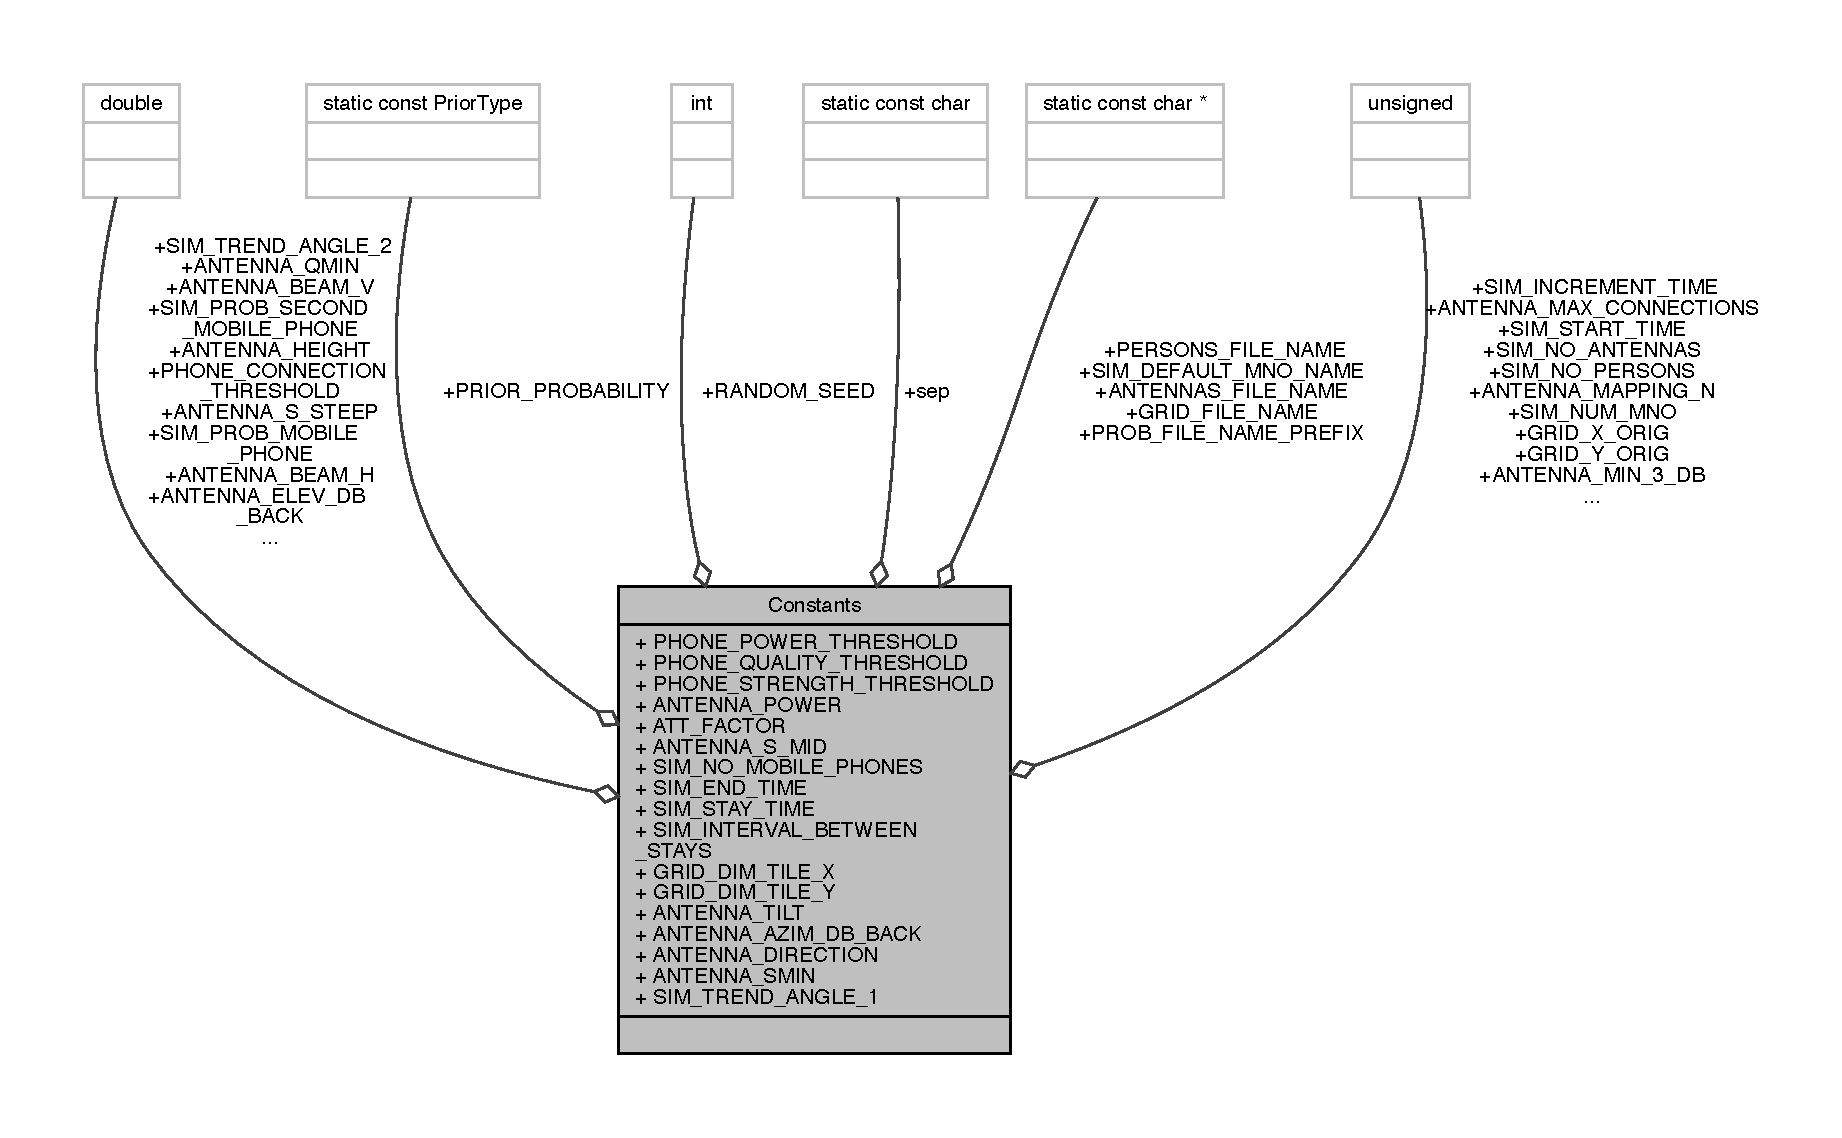
\includegraphics[width=350pt]{class_constants__coll__graph}
\end{center}
\end{figure}
\subsection*{Static Public Attributes}
\begin{DoxyCompactItemize}
\item 
static const double \hyperlink{class_constants_a1e95cbdc2db02f6147ddf8ac61a428ab}{P\+H\+O\+N\+E\+\_\+\+P\+O\+W\+E\+R\+\_\+\+T\+H\+R\+E\+S\+H\+O\+LD}
\item 
static const double \hyperlink{class_constants_a2c8a9d965bae29c19ff18c8b80260982}{P\+H\+O\+N\+E\+\_\+\+Q\+U\+A\+L\+I\+T\+Y\+\_\+\+T\+H\+R\+E\+S\+H\+O\+LD}
\item 
static const double \hyperlink{class_constants_a24b6069c3365fb95c4b853129e4d4a3e}{P\+H\+O\+N\+E\+\_\+\+S\+T\+R\+E\+N\+G\+T\+H\+\_\+\+T\+H\+R\+E\+S\+H\+O\+LD}
\item 
static const double \hyperlink{class_constants_a1cbf0a4e111b9d2e13b33e771a342b4f}{P\+H\+O\+N\+E\+\_\+\+C\+O\+N\+N\+E\+C\+T\+I\+O\+N\+\_\+\+T\+H\+R\+E\+S\+H\+O\+LD}
\item 
static const double \hyperlink{class_constants_a3f6f3825098d8eb1dc8081158c46c48a}{A\+N\+T\+E\+N\+N\+A\+\_\+\+P\+O\+W\+ER}
\item 
static const double \hyperlink{class_constants_a3738ccd4e7931b93885bdedf98528293}{A\+T\+T\+\_\+\+F\+A\+C\+T\+OR}
\item 
static const unsigned long \hyperlink{class_constants_af89a10a7d59ac020b1fa06cf673ef01f}{A\+N\+T\+E\+N\+N\+A\+\_\+\+M\+A\+X\+\_\+\+C\+O\+N\+N\+E\+C\+T\+I\+O\+NS}
\item 
static const double \hyperlink{class_constants_aea09e28749c0da58a4c831f9eabea773}{A\+N\+T\+E\+N\+N\+A\+\_\+\+S\+\_\+\+M\+ID}
\item 
static const double \hyperlink{class_constants_ae4b1b2c15d1e5bbb76464c03036c6baa}{A\+N\+T\+E\+N\+N\+A\+\_\+\+S\+\_\+\+S\+T\+E\+EP}
\item 
static const unsigned long \hyperlink{class_constants_a627fe53a717da1ca017b2467fb1dd4df}{S\+I\+M\+\_\+\+N\+O\+\_\+\+P\+E\+R\+S\+O\+NS}
\item 
static const unsigned long \hyperlink{class_constants_a0f6bc08399ad62727732e08a65c3bd0f}{S\+I\+M\+\_\+\+N\+O\+\_\+\+A\+N\+T\+E\+N\+N\+AS}
\item 
static const unsigned long \hyperlink{class_constants_a7da9e25a998c58c4388cbd45411f4232}{S\+I\+M\+\_\+\+N\+O\+\_\+\+M\+O\+B\+I\+L\+E\+\_\+\+P\+H\+O\+N\+ES}
\item 
static const unsigned long \hyperlink{class_constants_ad8a2d4817d599fd4f608e474bf1052ba}{S\+I\+M\+\_\+\+S\+T\+A\+R\+T\+\_\+\+T\+I\+ME}
\item 
static const unsigned long \hyperlink{class_constants_affb253c69b40f5979cd07383245331b7}{S\+I\+M\+\_\+\+E\+N\+D\+\_\+\+T\+I\+ME}
\item 
static const unsigned long \hyperlink{class_constants_ae689749614ecdd38b50a014400138bc2}{S\+I\+M\+\_\+\+I\+N\+C\+R\+E\+M\+E\+N\+T\+\_\+\+T\+I\+ME}
\item 
static const unsigned long \hyperlink{class_constants_a885a54aa8b2d13632ae3e8ff8e7664fb}{S\+I\+M\+\_\+\+S\+T\+A\+Y\+\_\+\+T\+I\+ME}
\item 
static const unsigned long \hyperlink{class_constants_a396cc1e9abbdf0a536886ebfd6b28045}{S\+I\+M\+\_\+\+I\+N\+T\+E\+R\+V\+A\+L\+\_\+\+B\+E\+T\+W\+E\+E\+N\+\_\+\+S\+T\+A\+YS}
\item 
static const char \hyperlink{class_constants_afc927f63cc5fbb912114d6b0f28b8b4f}{sep}
\item 
static const char $\ast$ \hyperlink{class_constants_aa2fd1c5551c8dab10dc1bd4c0cd0db8f}{G\+R\+I\+D\+\_\+\+F\+I\+L\+E\+\_\+\+N\+A\+ME}
\item 
static const unsigned long \hyperlink{class_constants_ac09062322e1ab9b6e1ca3a568b11c376}{G\+R\+I\+D\+\_\+\+X\+\_\+\+O\+R\+IG}
\item 
static const unsigned long \hyperlink{class_constants_ace48b30468931aaf452ab7a6daf573e0}{G\+R\+I\+D\+\_\+\+Y\+\_\+\+O\+R\+IG}
\item 
static const double \hyperlink{class_constants_a4400d3f97fa2e2be6091a8005efedd7f}{G\+R\+I\+D\+\_\+\+D\+I\+M\+\_\+\+T\+I\+L\+E\+\_\+X}
\item 
static const double \hyperlink{class_constants_a08f9273d844b68a74fd979d5a46d4918}{G\+R\+I\+D\+\_\+\+D\+I\+M\+\_\+\+T\+I\+L\+E\+\_\+Y}
\item 
static const char $\ast$ \hyperlink{class_constants_a3b2d3fc0ccc4636a51190bf5b297d72d}{P\+R\+O\+B\+\_\+\+F\+I\+L\+E\+\_\+\+N\+A\+M\+E\+\_\+\+P\+R\+E\+F\+IX}
\item 
static const char $\ast$ \hyperlink{class_constants_a2388516c40960223c0aef1610fd72312}{P\+E\+R\+S\+O\+N\+S\+\_\+\+F\+I\+L\+E\+\_\+\+N\+A\+ME}
\item 
static const char $\ast$ \hyperlink{class_constants_a23f758b23b88c7cfe23b278647671acb}{A\+N\+T\+E\+N\+N\+A\+S\+\_\+\+F\+I\+L\+E\+\_\+\+N\+A\+ME}
\item 
static const char $\ast$ \hyperlink{class_constants_a91fc37386abce571a0c7cd3f1b4b47c3}{O\+U\+T\+P\+U\+T\+\_\+\+D\+IR}
\item 
static const \hyperlink{_prior_type_8h_a61286c562e68de246982fc393a7c23a5}{Prior\+Type} \hyperlink{class_constants_a7b31976adc7ad0f3dbed86b205e1773d}{P\+R\+I\+O\+R\+\_\+\+P\+R\+O\+B\+A\+B\+I\+L\+I\+TY}
\item 
static const double \hyperlink{class_constants_adfe27efa61ae50b73c74b3f19c292625}{A\+N\+T\+E\+N\+N\+A\+\_\+\+H\+E\+I\+G\+HT}
\item 
static const double \hyperlink{class_constants_ad92a5c99071f0d843ee555e74c5f909a}{A\+N\+T\+E\+N\+N\+A\+\_\+\+T\+I\+LT}
\item 
static const double \hyperlink{class_constants_aa2030f2c0ec89fb7cc06b31bbb50793d}{A\+N\+T\+E\+N\+N\+A\+\_\+\+A\+Z\+I\+M\+\_\+\+D\+B\+\_\+\+B\+A\+CK}
\item 
static const double \hyperlink{class_constants_a8efdd6e1f2a25c24cb6dbff363e2d61a}{A\+N\+T\+E\+N\+N\+A\+\_\+\+E\+L\+E\+V\+\_\+\+D\+B\+\_\+\+B\+A\+CK}
\item 
static const double \hyperlink{class_constants_a4e4a0a48ad06c458ae4f3e6d0e4e6608}{A\+N\+T\+E\+N\+N\+A\+\_\+\+B\+E\+A\+M\+\_\+H}
\item 
static const double \hyperlink{class_constants_a2389355f6184d3b7903e154b46d069f5}{A\+N\+T\+E\+N\+N\+A\+\_\+\+B\+E\+A\+M\+\_\+V}
\item 
static const double \hyperlink{class_constants_ad82a10e13ae9e1cbce1cef616e47df31}{A\+N\+T\+E\+N\+N\+A\+\_\+\+D\+I\+R\+E\+C\+T\+I\+ON}
\item 
static const unsigned int \hyperlink{class_constants_a5db3a5bad9c514c994e71063dee2a798}{A\+N\+T\+E\+N\+N\+A\+\_\+\+M\+A\+P\+P\+I\+N\+G\+\_\+N}
\item 
static const unsigned int \hyperlink{class_constants_a2bda61c04e204f4a1279338fb790e1f4}{A\+N\+T\+E\+N\+N\+A\+\_\+\+M\+I\+N\+\_\+3\+\_\+\+DB}
\item 
static const double \hyperlink{class_constants_af58b693e1ab4cdb1e83399eb0f2af647}{A\+N\+T\+E\+N\+N\+A\+\_\+\+S\+M\+IN}
\item 
static const double \hyperlink{class_constants_a9149aaac071422191e4417885fd42b07}{A\+N\+T\+E\+N\+N\+A\+\_\+\+Q\+M\+IN}
\item 
static const unsigned int \hyperlink{class_constants_a763bdd9401295d6b691c93cf580e562a}{S\+I\+M\+\_\+\+N\+U\+M\+\_\+\+M\+NO}
\item 
static const char $\ast$ \hyperlink{class_constants_a186cf83e20074a889823a7f36e50ad8c}{S\+I\+M\+\_\+\+D\+E\+F\+A\+U\+L\+T\+\_\+\+M\+N\+O\+\_\+\+N\+A\+ME}
\item 
static const double \hyperlink{class_constants_a8af75c6e731c2f425cce792b33786db7}{S\+I\+M\+\_\+\+P\+R\+O\+B\+\_\+\+M\+O\+B\+I\+L\+E\+\_\+\+P\+H\+O\+NE}
\item 
static const double \hyperlink{class_constants_aafd39df52173dca1074d8c92aa5f9649}{S\+I\+M\+\_\+\+P\+R\+O\+B\+\_\+\+S\+E\+C\+O\+N\+D\+\_\+\+M\+O\+B\+I\+L\+E\+\_\+\+P\+H\+O\+NE}
\item 
static const double \hyperlink{class_constants_a97968377c9a3cf2995c37aa63d3dd505}{S\+I\+M\+\_\+\+T\+R\+E\+N\+D\+\_\+\+A\+N\+G\+L\+E\+\_\+1}
\item 
static const double \hyperlink{class_constants_a1ec9cdffb9c58a2ff1cb60f64b056835}{S\+I\+M\+\_\+\+T\+R\+E\+N\+D\+\_\+\+A\+N\+G\+L\+E\+\_\+2}
\item 
static const int \hyperlink{class_constants_ac80eccfaa8e498ad3fc6ea0a2c3d38a0}{R\+A\+N\+D\+O\+M\+\_\+\+S\+E\+ED}
\end{DoxyCompactItemize}


\subsection{Detailed Description}
These are some constants used in the process of the simulation, most of them are only used for testing and rapid development of some methods, the real values of the parameters being read from the configuration files. 

\subsection{Member Data Documentation}
\mbox{\Hypertarget{class_constants_aa2030f2c0ec89fb7cc06b31bbb50793d}\label{class_constants_aa2030f2c0ec89fb7cc06b31bbb50793d}} 
\index{Constants@{Constants}!A\+N\+T\+E\+N\+N\+A\+\_\+\+A\+Z\+I\+M\+\_\+\+D\+B\+\_\+\+B\+A\+CK@{A\+N\+T\+E\+N\+N\+A\+\_\+\+A\+Z\+I\+M\+\_\+\+D\+B\+\_\+\+B\+A\+CK}}
\index{A\+N\+T\+E\+N\+N\+A\+\_\+\+A\+Z\+I\+M\+\_\+\+D\+B\+\_\+\+B\+A\+CK@{A\+N\+T\+E\+N\+N\+A\+\_\+\+A\+Z\+I\+M\+\_\+\+D\+B\+\_\+\+B\+A\+CK}!Constants@{Constants}}
\subsubsection{\texorpdfstring{A\+N\+T\+E\+N\+N\+A\+\_\+\+A\+Z\+I\+M\+\_\+\+D\+B\+\_\+\+B\+A\+CK}{ANTENNA\_AZIM\_DB\_BACK}}
{\footnotesize\ttfamily const double Constants\+::\+A\+N\+T\+E\+N\+N\+A\+\_\+\+A\+Z\+I\+M\+\_\+\+D\+B\+\_\+\+B\+A\+CK\hspace{0.3cm}{\ttfamily [static]}}

\mbox{\Hypertarget{class_constants_a4e4a0a48ad06c458ae4f3e6d0e4e6608}\label{class_constants_a4e4a0a48ad06c458ae4f3e6d0e4e6608}} 
\index{Constants@{Constants}!A\+N\+T\+E\+N\+N\+A\+\_\+\+B\+E\+A\+M\+\_\+H@{A\+N\+T\+E\+N\+N\+A\+\_\+\+B\+E\+A\+M\+\_\+H}}
\index{A\+N\+T\+E\+N\+N\+A\+\_\+\+B\+E\+A\+M\+\_\+H@{A\+N\+T\+E\+N\+N\+A\+\_\+\+B\+E\+A\+M\+\_\+H}!Constants@{Constants}}
\subsubsection{\texorpdfstring{A\+N\+T\+E\+N\+N\+A\+\_\+\+B\+E\+A\+M\+\_\+H}{ANTENNA\_BEAM\_H}}
{\footnotesize\ttfamily const double Constants\+::\+A\+N\+T\+E\+N\+N\+A\+\_\+\+B\+E\+A\+M\+\_\+H\hspace{0.3cm}{\ttfamily [static]}}

\mbox{\Hypertarget{class_constants_a2389355f6184d3b7903e154b46d069f5}\label{class_constants_a2389355f6184d3b7903e154b46d069f5}} 
\index{Constants@{Constants}!A\+N\+T\+E\+N\+N\+A\+\_\+\+B\+E\+A\+M\+\_\+V@{A\+N\+T\+E\+N\+N\+A\+\_\+\+B\+E\+A\+M\+\_\+V}}
\index{A\+N\+T\+E\+N\+N\+A\+\_\+\+B\+E\+A\+M\+\_\+V@{A\+N\+T\+E\+N\+N\+A\+\_\+\+B\+E\+A\+M\+\_\+V}!Constants@{Constants}}
\subsubsection{\texorpdfstring{A\+N\+T\+E\+N\+N\+A\+\_\+\+B\+E\+A\+M\+\_\+V}{ANTENNA\_BEAM\_V}}
{\footnotesize\ttfamily const double Constants\+::\+A\+N\+T\+E\+N\+N\+A\+\_\+\+B\+E\+A\+M\+\_\+V\hspace{0.3cm}{\ttfamily [static]}}

\mbox{\Hypertarget{class_constants_ad82a10e13ae9e1cbce1cef616e47df31}\label{class_constants_ad82a10e13ae9e1cbce1cef616e47df31}} 
\index{Constants@{Constants}!A\+N\+T\+E\+N\+N\+A\+\_\+\+D\+I\+R\+E\+C\+T\+I\+ON@{A\+N\+T\+E\+N\+N\+A\+\_\+\+D\+I\+R\+E\+C\+T\+I\+ON}}
\index{A\+N\+T\+E\+N\+N\+A\+\_\+\+D\+I\+R\+E\+C\+T\+I\+ON@{A\+N\+T\+E\+N\+N\+A\+\_\+\+D\+I\+R\+E\+C\+T\+I\+ON}!Constants@{Constants}}
\subsubsection{\texorpdfstring{A\+N\+T\+E\+N\+N\+A\+\_\+\+D\+I\+R\+E\+C\+T\+I\+ON}{ANTENNA\_DIRECTION}}
{\footnotesize\ttfamily const double Constants\+::\+A\+N\+T\+E\+N\+N\+A\+\_\+\+D\+I\+R\+E\+C\+T\+I\+ON\hspace{0.3cm}{\ttfamily [static]}}

\mbox{\Hypertarget{class_constants_a8efdd6e1f2a25c24cb6dbff363e2d61a}\label{class_constants_a8efdd6e1f2a25c24cb6dbff363e2d61a}} 
\index{Constants@{Constants}!A\+N\+T\+E\+N\+N\+A\+\_\+\+E\+L\+E\+V\+\_\+\+D\+B\+\_\+\+B\+A\+CK@{A\+N\+T\+E\+N\+N\+A\+\_\+\+E\+L\+E\+V\+\_\+\+D\+B\+\_\+\+B\+A\+CK}}
\index{A\+N\+T\+E\+N\+N\+A\+\_\+\+E\+L\+E\+V\+\_\+\+D\+B\+\_\+\+B\+A\+CK@{A\+N\+T\+E\+N\+N\+A\+\_\+\+E\+L\+E\+V\+\_\+\+D\+B\+\_\+\+B\+A\+CK}!Constants@{Constants}}
\subsubsection{\texorpdfstring{A\+N\+T\+E\+N\+N\+A\+\_\+\+E\+L\+E\+V\+\_\+\+D\+B\+\_\+\+B\+A\+CK}{ANTENNA\_ELEV\_DB\_BACK}}
{\footnotesize\ttfamily const double Constants\+::\+A\+N\+T\+E\+N\+N\+A\+\_\+\+E\+L\+E\+V\+\_\+\+D\+B\+\_\+\+B\+A\+CK\hspace{0.3cm}{\ttfamily [static]}}

\mbox{\Hypertarget{class_constants_adfe27efa61ae50b73c74b3f19c292625}\label{class_constants_adfe27efa61ae50b73c74b3f19c292625}} 
\index{Constants@{Constants}!A\+N\+T\+E\+N\+N\+A\+\_\+\+H\+E\+I\+G\+HT@{A\+N\+T\+E\+N\+N\+A\+\_\+\+H\+E\+I\+G\+HT}}
\index{A\+N\+T\+E\+N\+N\+A\+\_\+\+H\+E\+I\+G\+HT@{A\+N\+T\+E\+N\+N\+A\+\_\+\+H\+E\+I\+G\+HT}!Constants@{Constants}}
\subsubsection{\texorpdfstring{A\+N\+T\+E\+N\+N\+A\+\_\+\+H\+E\+I\+G\+HT}{ANTENNA\_HEIGHT}}
{\footnotesize\ttfamily const double Constants\+::\+A\+N\+T\+E\+N\+N\+A\+\_\+\+H\+E\+I\+G\+HT\hspace{0.3cm}{\ttfamily [static]}}

the antenna height \mbox{\Hypertarget{class_constants_a5db3a5bad9c514c994e71063dee2a798}\label{class_constants_a5db3a5bad9c514c994e71063dee2a798}} 
\index{Constants@{Constants}!A\+N\+T\+E\+N\+N\+A\+\_\+\+M\+A\+P\+P\+I\+N\+G\+\_\+N@{A\+N\+T\+E\+N\+N\+A\+\_\+\+M\+A\+P\+P\+I\+N\+G\+\_\+N}}
\index{A\+N\+T\+E\+N\+N\+A\+\_\+\+M\+A\+P\+P\+I\+N\+G\+\_\+N@{A\+N\+T\+E\+N\+N\+A\+\_\+\+M\+A\+P\+P\+I\+N\+G\+\_\+N}!Constants@{Constants}}
\subsubsection{\texorpdfstring{A\+N\+T\+E\+N\+N\+A\+\_\+\+M\+A\+P\+P\+I\+N\+G\+\_\+N}{ANTENNA\_MAPPING\_N}}
{\footnotesize\ttfamily const unsigned int Constants\+::\+A\+N\+T\+E\+N\+N\+A\+\_\+\+M\+A\+P\+P\+I\+N\+G\+\_\+N\hspace{0.3cm}{\ttfamily [static]}}

\mbox{\Hypertarget{class_constants_af89a10a7d59ac020b1fa06cf673ef01f}\label{class_constants_af89a10a7d59ac020b1fa06cf673ef01f}} 
\index{Constants@{Constants}!A\+N\+T\+E\+N\+N\+A\+\_\+\+M\+A\+X\+\_\+\+C\+O\+N\+N\+E\+C\+T\+I\+O\+NS@{A\+N\+T\+E\+N\+N\+A\+\_\+\+M\+A\+X\+\_\+\+C\+O\+N\+N\+E\+C\+T\+I\+O\+NS}}
\index{A\+N\+T\+E\+N\+N\+A\+\_\+\+M\+A\+X\+\_\+\+C\+O\+N\+N\+E\+C\+T\+I\+O\+NS@{A\+N\+T\+E\+N\+N\+A\+\_\+\+M\+A\+X\+\_\+\+C\+O\+N\+N\+E\+C\+T\+I\+O\+NS}!Constants@{Constants}}
\subsubsection{\texorpdfstring{A\+N\+T\+E\+N\+N\+A\+\_\+\+M\+A\+X\+\_\+\+C\+O\+N\+N\+E\+C\+T\+I\+O\+NS}{ANTENNA\_MAX\_CONNECTIONS}}
{\footnotesize\ttfamily const unsigned long Constants\+::\+A\+N\+T\+E\+N\+N\+A\+\_\+\+M\+A\+X\+\_\+\+C\+O\+N\+N\+E\+C\+T\+I\+O\+NS\hspace{0.3cm}{\ttfamily [static]}}

The maximum number of devices an antenna can connect. \mbox{\Hypertarget{class_constants_a2bda61c04e204f4a1279338fb790e1f4}\label{class_constants_a2bda61c04e204f4a1279338fb790e1f4}} 
\index{Constants@{Constants}!A\+N\+T\+E\+N\+N\+A\+\_\+\+M\+I\+N\+\_\+3\+\_\+\+DB@{A\+N\+T\+E\+N\+N\+A\+\_\+\+M\+I\+N\+\_\+3\+\_\+\+DB}}
\index{A\+N\+T\+E\+N\+N\+A\+\_\+\+M\+I\+N\+\_\+3\+\_\+\+DB@{A\+N\+T\+E\+N\+N\+A\+\_\+\+M\+I\+N\+\_\+3\+\_\+\+DB}!Constants@{Constants}}
\subsubsection{\texorpdfstring{A\+N\+T\+E\+N\+N\+A\+\_\+\+M\+I\+N\+\_\+3\+\_\+\+DB}{ANTENNA\_MIN\_3\_DB}}
{\footnotesize\ttfamily const unsigned int Constants\+::\+A\+N\+T\+E\+N\+N\+A\+\_\+\+M\+I\+N\+\_\+3\+\_\+\+DB\hspace{0.3cm}{\ttfamily [static]}}

\mbox{\Hypertarget{class_constants_a3f6f3825098d8eb1dc8081158c46c48a}\label{class_constants_a3f6f3825098d8eb1dc8081158c46c48a}} 
\index{Constants@{Constants}!A\+N\+T\+E\+N\+N\+A\+\_\+\+P\+O\+W\+ER@{A\+N\+T\+E\+N\+N\+A\+\_\+\+P\+O\+W\+ER}}
\index{A\+N\+T\+E\+N\+N\+A\+\_\+\+P\+O\+W\+ER@{A\+N\+T\+E\+N\+N\+A\+\_\+\+P\+O\+W\+ER}!Constants@{Constants}}
\subsubsection{\texorpdfstring{A\+N\+T\+E\+N\+N\+A\+\_\+\+P\+O\+W\+ER}{ANTENNA\_POWER}}
{\footnotesize\ttfamily const double Constants\+::\+A\+N\+T\+E\+N\+N\+A\+\_\+\+P\+O\+W\+ER\hspace{0.3cm}{\ttfamily [static]}}

\hyperlink{class_antenna}{Antenna} power in Watts. \mbox{\Hypertarget{class_constants_a9149aaac071422191e4417885fd42b07}\label{class_constants_a9149aaac071422191e4417885fd42b07}} 
\index{Constants@{Constants}!A\+N\+T\+E\+N\+N\+A\+\_\+\+Q\+M\+IN@{A\+N\+T\+E\+N\+N\+A\+\_\+\+Q\+M\+IN}}
\index{A\+N\+T\+E\+N\+N\+A\+\_\+\+Q\+M\+IN@{A\+N\+T\+E\+N\+N\+A\+\_\+\+Q\+M\+IN}!Constants@{Constants}}
\subsubsection{\texorpdfstring{A\+N\+T\+E\+N\+N\+A\+\_\+\+Q\+M\+IN}{ANTENNA\_QMIN}}
{\footnotesize\ttfamily const double Constants\+::\+A\+N\+T\+E\+N\+N\+A\+\_\+\+Q\+M\+IN\hspace{0.3cm}{\ttfamily [static]}}

\mbox{\Hypertarget{class_constants_aea09e28749c0da58a4c831f9eabea773}\label{class_constants_aea09e28749c0da58a4c831f9eabea773}} 
\index{Constants@{Constants}!A\+N\+T\+E\+N\+N\+A\+\_\+\+S\+\_\+\+M\+ID@{A\+N\+T\+E\+N\+N\+A\+\_\+\+S\+\_\+\+M\+ID}}
\index{A\+N\+T\+E\+N\+N\+A\+\_\+\+S\+\_\+\+M\+ID@{A\+N\+T\+E\+N\+N\+A\+\_\+\+S\+\_\+\+M\+ID}!Constants@{Constants}}
\subsubsection{\texorpdfstring{A\+N\+T\+E\+N\+N\+A\+\_\+\+S\+\_\+\+M\+ID}{ANTENNA\_S\_MID}}
{\footnotesize\ttfamily const double Constants\+::\+A\+N\+T\+E\+N\+N\+A\+\_\+\+S\+\_\+\+M\+ID\hspace{0.3cm}{\ttfamily [static]}}

The Smid parameter of an antenna \mbox{\Hypertarget{class_constants_ae4b1b2c15d1e5bbb76464c03036c6baa}\label{class_constants_ae4b1b2c15d1e5bbb76464c03036c6baa}} 
\index{Constants@{Constants}!A\+N\+T\+E\+N\+N\+A\+\_\+\+S\+\_\+\+S\+T\+E\+EP@{A\+N\+T\+E\+N\+N\+A\+\_\+\+S\+\_\+\+S\+T\+E\+EP}}
\index{A\+N\+T\+E\+N\+N\+A\+\_\+\+S\+\_\+\+S\+T\+E\+EP@{A\+N\+T\+E\+N\+N\+A\+\_\+\+S\+\_\+\+S\+T\+E\+EP}!Constants@{Constants}}
\subsubsection{\texorpdfstring{A\+N\+T\+E\+N\+N\+A\+\_\+\+S\+\_\+\+S\+T\+E\+EP}{ANTENNA\_S\_STEEP}}
{\footnotesize\ttfamily const double Constants\+::\+A\+N\+T\+E\+N\+N\+A\+\_\+\+S\+\_\+\+S\+T\+E\+EP\hspace{0.3cm}{\ttfamily [static]}}

The Sstepp parameter of an antenna \mbox{\Hypertarget{class_constants_af58b693e1ab4cdb1e83399eb0f2af647}\label{class_constants_af58b693e1ab4cdb1e83399eb0f2af647}} 
\index{Constants@{Constants}!A\+N\+T\+E\+N\+N\+A\+\_\+\+S\+M\+IN@{A\+N\+T\+E\+N\+N\+A\+\_\+\+S\+M\+IN}}
\index{A\+N\+T\+E\+N\+N\+A\+\_\+\+S\+M\+IN@{A\+N\+T\+E\+N\+N\+A\+\_\+\+S\+M\+IN}!Constants@{Constants}}
\subsubsection{\texorpdfstring{A\+N\+T\+E\+N\+N\+A\+\_\+\+S\+M\+IN}{ANTENNA\_SMIN}}
{\footnotesize\ttfamily const double Constants\+::\+A\+N\+T\+E\+N\+N\+A\+\_\+\+S\+M\+IN\hspace{0.3cm}{\ttfamily [static]}}

\mbox{\Hypertarget{class_constants_ad92a5c99071f0d843ee555e74c5f909a}\label{class_constants_ad92a5c99071f0d843ee555e74c5f909a}} 
\index{Constants@{Constants}!A\+N\+T\+E\+N\+N\+A\+\_\+\+T\+I\+LT@{A\+N\+T\+E\+N\+N\+A\+\_\+\+T\+I\+LT}}
\index{A\+N\+T\+E\+N\+N\+A\+\_\+\+T\+I\+LT@{A\+N\+T\+E\+N\+N\+A\+\_\+\+T\+I\+LT}!Constants@{Constants}}
\subsubsection{\texorpdfstring{A\+N\+T\+E\+N\+N\+A\+\_\+\+T\+I\+LT}{ANTENNA\_TILT}}
{\footnotesize\ttfamily const double Constants\+::\+A\+N\+T\+E\+N\+N\+A\+\_\+\+T\+I\+LT\hspace{0.3cm}{\ttfamily [static]}}

\mbox{\Hypertarget{class_constants_a23f758b23b88c7cfe23b278647671acb}\label{class_constants_a23f758b23b88c7cfe23b278647671acb}} 
\index{Constants@{Constants}!A\+N\+T\+E\+N\+N\+A\+S\+\_\+\+F\+I\+L\+E\+\_\+\+N\+A\+ME@{A\+N\+T\+E\+N\+N\+A\+S\+\_\+\+F\+I\+L\+E\+\_\+\+N\+A\+ME}}
\index{A\+N\+T\+E\+N\+N\+A\+S\+\_\+\+F\+I\+L\+E\+\_\+\+N\+A\+ME@{A\+N\+T\+E\+N\+N\+A\+S\+\_\+\+F\+I\+L\+E\+\_\+\+N\+A\+ME}!Constants@{Constants}}
\subsubsection{\texorpdfstring{A\+N\+T\+E\+N\+N\+A\+S\+\_\+\+F\+I\+L\+E\+\_\+\+N\+A\+ME}{ANTENNAS\_FILE\_NAME}}
{\footnotesize\ttfamily const char$\ast$ Constants\+::\+A\+N\+T\+E\+N\+N\+A\+S\+\_\+\+F\+I\+L\+E\+\_\+\+N\+A\+ME\hspace{0.3cm}{\ttfamily [static]}}

The name of the file where the exact positions of the antennas are saved during simulation. They are needed for later analysis. \mbox{\Hypertarget{class_constants_a3738ccd4e7931b93885bdedf98528293}\label{class_constants_a3738ccd4e7931b93885bdedf98528293}} 
\index{Constants@{Constants}!A\+T\+T\+\_\+\+F\+A\+C\+T\+OR@{A\+T\+T\+\_\+\+F\+A\+C\+T\+OR}}
\index{A\+T\+T\+\_\+\+F\+A\+C\+T\+OR@{A\+T\+T\+\_\+\+F\+A\+C\+T\+OR}!Constants@{Constants}}
\subsubsection{\texorpdfstring{A\+T\+T\+\_\+\+F\+A\+C\+T\+OR}{ATT\_FACTOR}}
{\footnotesize\ttfamily const double Constants\+::\+A\+T\+T\+\_\+\+F\+A\+C\+T\+OR\hspace{0.3cm}{\ttfamily [static]}}

Attenuation factor of the signal. It usually takes values between 2 in open field and 6 inside buildings \mbox{\Hypertarget{class_constants_a4400d3f97fa2e2be6091a8005efedd7f}\label{class_constants_a4400d3f97fa2e2be6091a8005efedd7f}} 
\index{Constants@{Constants}!G\+R\+I\+D\+\_\+\+D\+I\+M\+\_\+\+T\+I\+L\+E\+\_\+X@{G\+R\+I\+D\+\_\+\+D\+I\+M\+\_\+\+T\+I\+L\+E\+\_\+X}}
\index{G\+R\+I\+D\+\_\+\+D\+I\+M\+\_\+\+T\+I\+L\+E\+\_\+X@{G\+R\+I\+D\+\_\+\+D\+I\+M\+\_\+\+T\+I\+L\+E\+\_\+X}!Constants@{Constants}}
\subsubsection{\texorpdfstring{G\+R\+I\+D\+\_\+\+D\+I\+M\+\_\+\+T\+I\+L\+E\+\_\+X}{GRID\_DIM\_TILE\_X}}
{\footnotesize\ttfamily const double Constants\+::\+G\+R\+I\+D\+\_\+\+D\+I\+M\+\_\+\+T\+I\+L\+E\+\_\+X\hspace{0.3cm}{\ttfamily [static]}}

\mbox{\Hypertarget{class_constants_a08f9273d844b68a74fd979d5a46d4918}\label{class_constants_a08f9273d844b68a74fd979d5a46d4918}} 
\index{Constants@{Constants}!G\+R\+I\+D\+\_\+\+D\+I\+M\+\_\+\+T\+I\+L\+E\+\_\+Y@{G\+R\+I\+D\+\_\+\+D\+I\+M\+\_\+\+T\+I\+L\+E\+\_\+Y}}
\index{G\+R\+I\+D\+\_\+\+D\+I\+M\+\_\+\+T\+I\+L\+E\+\_\+Y@{G\+R\+I\+D\+\_\+\+D\+I\+M\+\_\+\+T\+I\+L\+E\+\_\+Y}!Constants@{Constants}}
\subsubsection{\texorpdfstring{G\+R\+I\+D\+\_\+\+D\+I\+M\+\_\+\+T\+I\+L\+E\+\_\+Y}{GRID\_DIM\_TILE\_Y}}
{\footnotesize\ttfamily const double Constants\+::\+G\+R\+I\+D\+\_\+\+D\+I\+M\+\_\+\+T\+I\+L\+E\+\_\+Y\hspace{0.3cm}{\ttfamily [static]}}

\mbox{\Hypertarget{class_constants_aa2fd1c5551c8dab10dc1bd4c0cd0db8f}\label{class_constants_aa2fd1c5551c8dab10dc1bd4c0cd0db8f}} 
\index{Constants@{Constants}!G\+R\+I\+D\+\_\+\+F\+I\+L\+E\+\_\+\+N\+A\+ME@{G\+R\+I\+D\+\_\+\+F\+I\+L\+E\+\_\+\+N\+A\+ME}}
\index{G\+R\+I\+D\+\_\+\+F\+I\+L\+E\+\_\+\+N\+A\+ME@{G\+R\+I\+D\+\_\+\+F\+I\+L\+E\+\_\+\+N\+A\+ME}!Constants@{Constants}}
\subsubsection{\texorpdfstring{G\+R\+I\+D\+\_\+\+F\+I\+L\+E\+\_\+\+N\+A\+ME}{GRID\_FILE\_NAME}}
{\footnotesize\ttfamily const char$\ast$ Constants\+::\+G\+R\+I\+D\+\_\+\+F\+I\+L\+E\+\_\+\+N\+A\+ME\hspace{0.3cm}{\ttfamily [static]}}

The name of the file where the description of the grid is saved \mbox{\Hypertarget{class_constants_ac09062322e1ab9b6e1ca3a568b11c376}\label{class_constants_ac09062322e1ab9b6e1ca3a568b11c376}} 
\index{Constants@{Constants}!G\+R\+I\+D\+\_\+\+X\+\_\+\+O\+R\+IG@{G\+R\+I\+D\+\_\+\+X\+\_\+\+O\+R\+IG}}
\index{G\+R\+I\+D\+\_\+\+X\+\_\+\+O\+R\+IG@{G\+R\+I\+D\+\_\+\+X\+\_\+\+O\+R\+IG}!Constants@{Constants}}
\subsubsection{\texorpdfstring{G\+R\+I\+D\+\_\+\+X\+\_\+\+O\+R\+IG}{GRID\_X\_ORIG}}
{\footnotesize\ttfamily const unsigned long Constants\+::\+G\+R\+I\+D\+\_\+\+X\+\_\+\+O\+R\+IG\hspace{0.3cm}{\ttfamily [static]}}

\mbox{\Hypertarget{class_constants_ace48b30468931aaf452ab7a6daf573e0}\label{class_constants_ace48b30468931aaf452ab7a6daf573e0}} 
\index{Constants@{Constants}!G\+R\+I\+D\+\_\+\+Y\+\_\+\+O\+R\+IG@{G\+R\+I\+D\+\_\+\+Y\+\_\+\+O\+R\+IG}}
\index{G\+R\+I\+D\+\_\+\+Y\+\_\+\+O\+R\+IG@{G\+R\+I\+D\+\_\+\+Y\+\_\+\+O\+R\+IG}!Constants@{Constants}}
\subsubsection{\texorpdfstring{G\+R\+I\+D\+\_\+\+Y\+\_\+\+O\+R\+IG}{GRID\_Y\_ORIG}}
{\footnotesize\ttfamily const unsigned long Constants\+::\+G\+R\+I\+D\+\_\+\+Y\+\_\+\+O\+R\+IG\hspace{0.3cm}{\ttfamily [static]}}

\mbox{\Hypertarget{class_constants_a91fc37386abce571a0c7cd3f1b4b47c3}\label{class_constants_a91fc37386abce571a0c7cd3f1b4b47c3}} 
\index{Constants@{Constants}!O\+U\+T\+P\+U\+T\+\_\+\+D\+IR@{O\+U\+T\+P\+U\+T\+\_\+\+D\+IR}}
\index{O\+U\+T\+P\+U\+T\+\_\+\+D\+IR@{O\+U\+T\+P\+U\+T\+\_\+\+D\+IR}!Constants@{Constants}}
\subsubsection{\texorpdfstring{O\+U\+T\+P\+U\+T\+\_\+\+D\+IR}{OUTPUT\_DIR}}
{\footnotesize\ttfamily const char$\ast$ Constants\+::\+O\+U\+T\+P\+U\+T\+\_\+\+D\+IR\hspace{0.3cm}{\ttfamily [static]}}

The name of the folder where the output fle will be saved \mbox{\Hypertarget{class_constants_a2388516c40960223c0aef1610fd72312}\label{class_constants_a2388516c40960223c0aef1610fd72312}} 
\index{Constants@{Constants}!P\+E\+R\+S\+O\+N\+S\+\_\+\+F\+I\+L\+E\+\_\+\+N\+A\+ME@{P\+E\+R\+S\+O\+N\+S\+\_\+\+F\+I\+L\+E\+\_\+\+N\+A\+ME}}
\index{P\+E\+R\+S\+O\+N\+S\+\_\+\+F\+I\+L\+E\+\_\+\+N\+A\+ME@{P\+E\+R\+S\+O\+N\+S\+\_\+\+F\+I\+L\+E\+\_\+\+N\+A\+ME}!Constants@{Constants}}
\subsubsection{\texorpdfstring{P\+E\+R\+S\+O\+N\+S\+\_\+\+F\+I\+L\+E\+\_\+\+N\+A\+ME}{PERSONS\_FILE\_NAME}}
{\footnotesize\ttfamily const char$\ast$ Constants\+::\+P\+E\+R\+S\+O\+N\+S\+\_\+\+F\+I\+L\+E\+\_\+\+N\+A\+ME\hspace{0.3cm}{\ttfamily [static]}}

The name of the file where the exact positions of the persons are saved during simulation. They are needed for later analysis. \mbox{\Hypertarget{class_constants_a1cbf0a4e111b9d2e13b33e771a342b4f}\label{class_constants_a1cbf0a4e111b9d2e13b33e771a342b4f}} 
\index{Constants@{Constants}!P\+H\+O\+N\+E\+\_\+\+C\+O\+N\+N\+E\+C\+T\+I\+O\+N\+\_\+\+T\+H\+R\+E\+S\+H\+O\+LD@{P\+H\+O\+N\+E\+\_\+\+C\+O\+N\+N\+E\+C\+T\+I\+O\+N\+\_\+\+T\+H\+R\+E\+S\+H\+O\+LD}}
\index{P\+H\+O\+N\+E\+\_\+\+C\+O\+N\+N\+E\+C\+T\+I\+O\+N\+\_\+\+T\+H\+R\+E\+S\+H\+O\+LD@{P\+H\+O\+N\+E\+\_\+\+C\+O\+N\+N\+E\+C\+T\+I\+O\+N\+\_\+\+T\+H\+R\+E\+S\+H\+O\+LD}!Constants@{Constants}}
\subsubsection{\texorpdfstring{P\+H\+O\+N\+E\+\_\+\+C\+O\+N\+N\+E\+C\+T\+I\+O\+N\+\_\+\+T\+H\+R\+E\+S\+H\+O\+LD}{PHONE\_CONNECTION\_THRESHOLD}}
{\footnotesize\ttfamily const double Constants\+::\+P\+H\+O\+N\+E\+\_\+\+C\+O\+N\+N\+E\+C\+T\+I\+O\+N\+\_\+\+T\+H\+R\+E\+S\+H\+O\+LD\hspace{0.3cm}{\ttfamily [static]}}

This value is interpreted according to the connection type\+:
\begin{DoxyItemize}
\item if the connection uses power it is the minimum value of the signal power received by a phone not considered as noise. Below this value the signal is unusable and the connection between a mobile phone and an antenna is not possible.
\item if the connection uses signal quality it is the minimum value of the signal quality received by a phone not considered as noise. Below this value the signal is unusable and the connection between a mobile phone and an antenna is not possible.
\item if the connection uses signal strength it is the minimum value of the signal strength received by a phone not considered as noise. Below this value the signal is unusable and the connection between a mobile phone and an antenna is not possible. 
\end{DoxyItemize}\mbox{\Hypertarget{class_constants_a1e95cbdc2db02f6147ddf8ac61a428ab}\label{class_constants_a1e95cbdc2db02f6147ddf8ac61a428ab}} 
\index{Constants@{Constants}!P\+H\+O\+N\+E\+\_\+\+P\+O\+W\+E\+R\+\_\+\+T\+H\+R\+E\+S\+H\+O\+LD@{P\+H\+O\+N\+E\+\_\+\+P\+O\+W\+E\+R\+\_\+\+T\+H\+R\+E\+S\+H\+O\+LD}}
\index{P\+H\+O\+N\+E\+\_\+\+P\+O\+W\+E\+R\+\_\+\+T\+H\+R\+E\+S\+H\+O\+LD@{P\+H\+O\+N\+E\+\_\+\+P\+O\+W\+E\+R\+\_\+\+T\+H\+R\+E\+S\+H\+O\+LD}!Constants@{Constants}}
\subsubsection{\texorpdfstring{P\+H\+O\+N\+E\+\_\+\+P\+O\+W\+E\+R\+\_\+\+T\+H\+R\+E\+S\+H\+O\+LD}{PHONE\_POWER\_THRESHOLD}}
{\footnotesize\ttfamily const double Constants\+::\+P\+H\+O\+N\+E\+\_\+\+P\+O\+W\+E\+R\+\_\+\+T\+H\+R\+E\+S\+H\+O\+LD\hspace{0.3cm}{\ttfamily [static]}}

If the signal received by a mobile device has a power below this level, the signal is considered only noise and unusable. \mbox{\Hypertarget{class_constants_a2c8a9d965bae29c19ff18c8b80260982}\label{class_constants_a2c8a9d965bae29c19ff18c8b80260982}} 
\index{Constants@{Constants}!P\+H\+O\+N\+E\+\_\+\+Q\+U\+A\+L\+I\+T\+Y\+\_\+\+T\+H\+R\+E\+S\+H\+O\+LD@{P\+H\+O\+N\+E\+\_\+\+Q\+U\+A\+L\+I\+T\+Y\+\_\+\+T\+H\+R\+E\+S\+H\+O\+LD}}
\index{P\+H\+O\+N\+E\+\_\+\+Q\+U\+A\+L\+I\+T\+Y\+\_\+\+T\+H\+R\+E\+S\+H\+O\+LD@{P\+H\+O\+N\+E\+\_\+\+Q\+U\+A\+L\+I\+T\+Y\+\_\+\+T\+H\+R\+E\+S\+H\+O\+LD}!Constants@{Constants}}
\subsubsection{\texorpdfstring{P\+H\+O\+N\+E\+\_\+\+Q\+U\+A\+L\+I\+T\+Y\+\_\+\+T\+H\+R\+E\+S\+H\+O\+LD}{PHONE\_QUALITY\_THRESHOLD}}
{\footnotesize\ttfamily const double Constants\+::\+P\+H\+O\+N\+E\+\_\+\+Q\+U\+A\+L\+I\+T\+Y\+\_\+\+T\+H\+R\+E\+S\+H\+O\+LD\hspace{0.3cm}{\ttfamily [static]}}

If the signal received by a mobile device has a quality below this level, the signal is considered only noise and unusable. \mbox{\Hypertarget{class_constants_a24b6069c3365fb95c4b853129e4d4a3e}\label{class_constants_a24b6069c3365fb95c4b853129e4d4a3e}} 
\index{Constants@{Constants}!P\+H\+O\+N\+E\+\_\+\+S\+T\+R\+E\+N\+G\+T\+H\+\_\+\+T\+H\+R\+E\+S\+H\+O\+LD@{P\+H\+O\+N\+E\+\_\+\+S\+T\+R\+E\+N\+G\+T\+H\+\_\+\+T\+H\+R\+E\+S\+H\+O\+LD}}
\index{P\+H\+O\+N\+E\+\_\+\+S\+T\+R\+E\+N\+G\+T\+H\+\_\+\+T\+H\+R\+E\+S\+H\+O\+LD@{P\+H\+O\+N\+E\+\_\+\+S\+T\+R\+E\+N\+G\+T\+H\+\_\+\+T\+H\+R\+E\+S\+H\+O\+LD}!Constants@{Constants}}
\subsubsection{\texorpdfstring{P\+H\+O\+N\+E\+\_\+\+S\+T\+R\+E\+N\+G\+T\+H\+\_\+\+T\+H\+R\+E\+S\+H\+O\+LD}{PHONE\_STRENGTH\_THRESHOLD}}
{\footnotesize\ttfamily const double Constants\+::\+P\+H\+O\+N\+E\+\_\+\+S\+T\+R\+E\+N\+G\+T\+H\+\_\+\+T\+H\+R\+E\+S\+H\+O\+LD\hspace{0.3cm}{\ttfamily [static]}}

If the signal received by a mobile device has a quality below this level, the signal is considered only noise and unusable. \mbox{\Hypertarget{class_constants_a7b31976adc7ad0f3dbed86b205e1773d}\label{class_constants_a7b31976adc7ad0f3dbed86b205e1773d}} 
\index{Constants@{Constants}!P\+R\+I\+O\+R\+\_\+\+P\+R\+O\+B\+A\+B\+I\+L\+I\+TY@{P\+R\+I\+O\+R\+\_\+\+P\+R\+O\+B\+A\+B\+I\+L\+I\+TY}}
\index{P\+R\+I\+O\+R\+\_\+\+P\+R\+O\+B\+A\+B\+I\+L\+I\+TY@{P\+R\+I\+O\+R\+\_\+\+P\+R\+O\+B\+A\+B\+I\+L\+I\+TY}!Constants@{Constants}}
\subsubsection{\texorpdfstring{P\+R\+I\+O\+R\+\_\+\+P\+R\+O\+B\+A\+B\+I\+L\+I\+TY}{PRIOR\_PROBABILITY}}
{\footnotesize\ttfamily const \hyperlink{_prior_type_8h_a61286c562e68de246982fc393a7c23a5}{Prior\+Type} Constants\+::\+P\+R\+I\+O\+R\+\_\+\+P\+R\+O\+B\+A\+B\+I\+L\+I\+TY\hspace{0.3cm}{\ttfamily [static]}}

Indicates how the prior probability is computed\+: uniform, register, network \mbox{\Hypertarget{class_constants_a3b2d3fc0ccc4636a51190bf5b297d72d}\label{class_constants_a3b2d3fc0ccc4636a51190bf5b297d72d}} 
\index{Constants@{Constants}!P\+R\+O\+B\+\_\+\+F\+I\+L\+E\+\_\+\+N\+A\+M\+E\+\_\+\+P\+R\+E\+F\+IX@{P\+R\+O\+B\+\_\+\+F\+I\+L\+E\+\_\+\+N\+A\+M\+E\+\_\+\+P\+R\+E\+F\+IX}}
\index{P\+R\+O\+B\+\_\+\+F\+I\+L\+E\+\_\+\+N\+A\+M\+E\+\_\+\+P\+R\+E\+F\+IX@{P\+R\+O\+B\+\_\+\+F\+I\+L\+E\+\_\+\+N\+A\+M\+E\+\_\+\+P\+R\+E\+F\+IX}!Constants@{Constants}}
\subsubsection{\texorpdfstring{P\+R\+O\+B\+\_\+\+F\+I\+L\+E\+\_\+\+N\+A\+M\+E\+\_\+\+P\+R\+E\+F\+IX}{PROB\_FILE\_NAME\_PREFIX}}
{\footnotesize\ttfamily const char$\ast$ Constants\+::\+P\+R\+O\+B\+\_\+\+F\+I\+L\+E\+\_\+\+N\+A\+M\+E\+\_\+\+P\+R\+E\+F\+IX\hspace{0.3cm}{\ttfamily [static]}}

The name of the file where the probabilities of mobile phones locations are saved \mbox{\Hypertarget{class_constants_ac80eccfaa8e498ad3fc6ea0a2c3d38a0}\label{class_constants_ac80eccfaa8e498ad3fc6ea0a2c3d38a0}} 
\index{Constants@{Constants}!R\+A\+N\+D\+O\+M\+\_\+\+S\+E\+ED@{R\+A\+N\+D\+O\+M\+\_\+\+S\+E\+ED}}
\index{R\+A\+N\+D\+O\+M\+\_\+\+S\+E\+ED@{R\+A\+N\+D\+O\+M\+\_\+\+S\+E\+ED}!Constants@{Constants}}
\subsubsection{\texorpdfstring{R\+A\+N\+D\+O\+M\+\_\+\+S\+E\+ED}{RANDOM\_SEED}}
{\footnotesize\ttfamily const int Constants\+::\+R\+A\+N\+D\+O\+M\+\_\+\+S\+E\+ED\hspace{0.3cm}{\ttfamily [static]}}

\mbox{\Hypertarget{class_constants_afc927f63cc5fbb912114d6b0f28b8b4f}\label{class_constants_afc927f63cc5fbb912114d6b0f28b8b4f}} 
\index{Constants@{Constants}!sep@{sep}}
\index{sep@{sep}!Constants@{Constants}}
\subsubsection{\texorpdfstring{sep}{sep}}
{\footnotesize\ttfamily const char Constants\+::sep\hspace{0.3cm}{\ttfamily [static]}}

The separator used when information is saved in output files \mbox{\Hypertarget{class_constants_a186cf83e20074a889823a7f36e50ad8c}\label{class_constants_a186cf83e20074a889823a7f36e50ad8c}} 
\index{Constants@{Constants}!S\+I\+M\+\_\+\+D\+E\+F\+A\+U\+L\+T\+\_\+\+M\+N\+O\+\_\+\+N\+A\+ME@{S\+I\+M\+\_\+\+D\+E\+F\+A\+U\+L\+T\+\_\+\+M\+N\+O\+\_\+\+N\+A\+ME}}
\index{S\+I\+M\+\_\+\+D\+E\+F\+A\+U\+L\+T\+\_\+\+M\+N\+O\+\_\+\+N\+A\+ME@{S\+I\+M\+\_\+\+D\+E\+F\+A\+U\+L\+T\+\_\+\+M\+N\+O\+\_\+\+N\+A\+ME}!Constants@{Constants}}
\subsubsection{\texorpdfstring{S\+I\+M\+\_\+\+D\+E\+F\+A\+U\+L\+T\+\_\+\+M\+N\+O\+\_\+\+N\+A\+ME}{SIM\_DEFAULT\_MNO\_NAME}}
{\footnotesize\ttfamily const char$\ast$ Constants\+::\+S\+I\+M\+\_\+\+D\+E\+F\+A\+U\+L\+T\+\_\+\+M\+N\+O\+\_\+\+N\+A\+ME\hspace{0.3cm}{\ttfamily [static]}}

\mbox{\Hypertarget{class_constants_affb253c69b40f5979cd07383245331b7}\label{class_constants_affb253c69b40f5979cd07383245331b7}} 
\index{Constants@{Constants}!S\+I\+M\+\_\+\+E\+N\+D\+\_\+\+T\+I\+ME@{S\+I\+M\+\_\+\+E\+N\+D\+\_\+\+T\+I\+ME}}
\index{S\+I\+M\+\_\+\+E\+N\+D\+\_\+\+T\+I\+ME@{S\+I\+M\+\_\+\+E\+N\+D\+\_\+\+T\+I\+ME}!Constants@{Constants}}
\subsubsection{\texorpdfstring{S\+I\+M\+\_\+\+E\+N\+D\+\_\+\+T\+I\+ME}{SIM\_END\_TIME}}
{\footnotesize\ttfamily const unsigned long Constants\+::\+S\+I\+M\+\_\+\+E\+N\+D\+\_\+\+T\+I\+ME\hspace{0.3cm}{\ttfamily [static]}}

Default ending time of a simulation \mbox{\Hypertarget{class_constants_ae689749614ecdd38b50a014400138bc2}\label{class_constants_ae689749614ecdd38b50a014400138bc2}} 
\index{Constants@{Constants}!S\+I\+M\+\_\+\+I\+N\+C\+R\+E\+M\+E\+N\+T\+\_\+\+T\+I\+ME@{S\+I\+M\+\_\+\+I\+N\+C\+R\+E\+M\+E\+N\+T\+\_\+\+T\+I\+ME}}
\index{S\+I\+M\+\_\+\+I\+N\+C\+R\+E\+M\+E\+N\+T\+\_\+\+T\+I\+ME@{S\+I\+M\+\_\+\+I\+N\+C\+R\+E\+M\+E\+N\+T\+\_\+\+T\+I\+ME}!Constants@{Constants}}
\subsubsection{\texorpdfstring{S\+I\+M\+\_\+\+I\+N\+C\+R\+E\+M\+E\+N\+T\+\_\+\+T\+I\+ME}{SIM\_INCREMENT\_TIME}}
{\footnotesize\ttfamily const unsigned long Constants\+::\+S\+I\+M\+\_\+\+I\+N\+C\+R\+E\+M\+E\+N\+T\+\_\+\+T\+I\+ME\hspace{0.3cm}{\ttfamily [static]}}

Default time increment for a simulation \mbox{\Hypertarget{class_constants_a396cc1e9abbdf0a536886ebfd6b28045}\label{class_constants_a396cc1e9abbdf0a536886ebfd6b28045}} 
\index{Constants@{Constants}!S\+I\+M\+\_\+\+I\+N\+T\+E\+R\+V\+A\+L\+\_\+\+B\+E\+T\+W\+E\+E\+N\+\_\+\+S\+T\+A\+YS@{S\+I\+M\+\_\+\+I\+N\+T\+E\+R\+V\+A\+L\+\_\+\+B\+E\+T\+W\+E\+E\+N\+\_\+\+S\+T\+A\+YS}}
\index{S\+I\+M\+\_\+\+I\+N\+T\+E\+R\+V\+A\+L\+\_\+\+B\+E\+T\+W\+E\+E\+N\+\_\+\+S\+T\+A\+YS@{S\+I\+M\+\_\+\+I\+N\+T\+E\+R\+V\+A\+L\+\_\+\+B\+E\+T\+W\+E\+E\+N\+\_\+\+S\+T\+A\+YS}!Constants@{Constants}}
\subsubsection{\texorpdfstring{S\+I\+M\+\_\+\+I\+N\+T\+E\+R\+V\+A\+L\+\_\+\+B\+E\+T\+W\+E\+E\+N\+\_\+\+S\+T\+A\+YS}{SIM\_INTERVAL\_BETWEEN\_STAYS}}
{\footnotesize\ttfamily const unsigned long Constants\+::\+S\+I\+M\+\_\+\+I\+N\+T\+E\+R\+V\+A\+L\+\_\+\+B\+E\+T\+W\+E\+E\+N\+\_\+\+S\+T\+A\+YS\hspace{0.3cm}{\ttfamily [static]}}

\mbox{\Hypertarget{class_constants_a0f6bc08399ad62727732e08a65c3bd0f}\label{class_constants_a0f6bc08399ad62727732e08a65c3bd0f}} 
\index{Constants@{Constants}!S\+I\+M\+\_\+\+N\+O\+\_\+\+A\+N\+T\+E\+N\+N\+AS@{S\+I\+M\+\_\+\+N\+O\+\_\+\+A\+N\+T\+E\+N\+N\+AS}}
\index{S\+I\+M\+\_\+\+N\+O\+\_\+\+A\+N\+T\+E\+N\+N\+AS@{S\+I\+M\+\_\+\+N\+O\+\_\+\+A\+N\+T\+E\+N\+N\+AS}!Constants@{Constants}}
\subsubsection{\texorpdfstring{S\+I\+M\+\_\+\+N\+O\+\_\+\+A\+N\+T\+E\+N\+N\+AS}{SIM\_NO\_ANTENNAS}}
{\footnotesize\ttfamily const unsigned long Constants\+::\+S\+I\+M\+\_\+\+N\+O\+\_\+\+A\+N\+T\+E\+N\+N\+AS\hspace{0.3cm}{\ttfamily [static]}}

The number of antenna used for a simulation \mbox{\Hypertarget{class_constants_a7da9e25a998c58c4388cbd45411f4232}\label{class_constants_a7da9e25a998c58c4388cbd45411f4232}} 
\index{Constants@{Constants}!S\+I\+M\+\_\+\+N\+O\+\_\+\+M\+O\+B\+I\+L\+E\+\_\+\+P\+H\+O\+N\+ES@{S\+I\+M\+\_\+\+N\+O\+\_\+\+M\+O\+B\+I\+L\+E\+\_\+\+P\+H\+O\+N\+ES}}
\index{S\+I\+M\+\_\+\+N\+O\+\_\+\+M\+O\+B\+I\+L\+E\+\_\+\+P\+H\+O\+N\+ES@{S\+I\+M\+\_\+\+N\+O\+\_\+\+M\+O\+B\+I\+L\+E\+\_\+\+P\+H\+O\+N\+ES}!Constants@{Constants}}
\subsubsection{\texorpdfstring{S\+I\+M\+\_\+\+N\+O\+\_\+\+M\+O\+B\+I\+L\+E\+\_\+\+P\+H\+O\+N\+ES}{SIM\_NO\_MOBILE\_PHONES}}
{\footnotesize\ttfamily const unsigned long Constants\+::\+S\+I\+M\+\_\+\+N\+O\+\_\+\+M\+O\+B\+I\+L\+E\+\_\+\+P\+H\+O\+N\+ES\hspace{0.3cm}{\ttfamily [static]}}

The number of the mobile devices used for a simulation \mbox{\Hypertarget{class_constants_a627fe53a717da1ca017b2467fb1dd4df}\label{class_constants_a627fe53a717da1ca017b2467fb1dd4df}} 
\index{Constants@{Constants}!S\+I\+M\+\_\+\+N\+O\+\_\+\+P\+E\+R\+S\+O\+NS@{S\+I\+M\+\_\+\+N\+O\+\_\+\+P\+E\+R\+S\+O\+NS}}
\index{S\+I\+M\+\_\+\+N\+O\+\_\+\+P\+E\+R\+S\+O\+NS@{S\+I\+M\+\_\+\+N\+O\+\_\+\+P\+E\+R\+S\+O\+NS}!Constants@{Constants}}
\subsubsection{\texorpdfstring{S\+I\+M\+\_\+\+N\+O\+\_\+\+P\+E\+R\+S\+O\+NS}{SIM\_NO\_PERSONS}}
{\footnotesize\ttfamily const unsigned long Constants\+::\+S\+I\+M\+\_\+\+N\+O\+\_\+\+P\+E\+R\+S\+O\+NS\hspace{0.3cm}{\ttfamily [static]}}

The number of persons used for a simulation \mbox{\Hypertarget{class_constants_a763bdd9401295d6b691c93cf580e562a}\label{class_constants_a763bdd9401295d6b691c93cf580e562a}} 
\index{Constants@{Constants}!S\+I\+M\+\_\+\+N\+U\+M\+\_\+\+M\+NO@{S\+I\+M\+\_\+\+N\+U\+M\+\_\+\+M\+NO}}
\index{S\+I\+M\+\_\+\+N\+U\+M\+\_\+\+M\+NO@{S\+I\+M\+\_\+\+N\+U\+M\+\_\+\+M\+NO}!Constants@{Constants}}
\subsubsection{\texorpdfstring{S\+I\+M\+\_\+\+N\+U\+M\+\_\+\+M\+NO}{SIM\_NUM\_MNO}}
{\footnotesize\ttfamily const unsigned int Constants\+::\+S\+I\+M\+\_\+\+N\+U\+M\+\_\+\+M\+NO\hspace{0.3cm}{\ttfamily [static]}}

\mbox{\Hypertarget{class_constants_a8af75c6e731c2f425cce792b33786db7}\label{class_constants_a8af75c6e731c2f425cce792b33786db7}} 
\index{Constants@{Constants}!S\+I\+M\+\_\+\+P\+R\+O\+B\+\_\+\+M\+O\+B\+I\+L\+E\+\_\+\+P\+H\+O\+NE@{S\+I\+M\+\_\+\+P\+R\+O\+B\+\_\+\+M\+O\+B\+I\+L\+E\+\_\+\+P\+H\+O\+NE}}
\index{S\+I\+M\+\_\+\+P\+R\+O\+B\+\_\+\+M\+O\+B\+I\+L\+E\+\_\+\+P\+H\+O\+NE@{S\+I\+M\+\_\+\+P\+R\+O\+B\+\_\+\+M\+O\+B\+I\+L\+E\+\_\+\+P\+H\+O\+NE}!Constants@{Constants}}
\subsubsection{\texorpdfstring{S\+I\+M\+\_\+\+P\+R\+O\+B\+\_\+\+M\+O\+B\+I\+L\+E\+\_\+\+P\+H\+O\+NE}{SIM\_PROB\_MOBILE\_PHONE}}
{\footnotesize\ttfamily const double Constants\+::\+S\+I\+M\+\_\+\+P\+R\+O\+B\+\_\+\+M\+O\+B\+I\+L\+E\+\_\+\+P\+H\+O\+NE\hspace{0.3cm}{\ttfamily [static]}}

\mbox{\Hypertarget{class_constants_aafd39df52173dca1074d8c92aa5f9649}\label{class_constants_aafd39df52173dca1074d8c92aa5f9649}} 
\index{Constants@{Constants}!S\+I\+M\+\_\+\+P\+R\+O\+B\+\_\+\+S\+E\+C\+O\+N\+D\+\_\+\+M\+O\+B\+I\+L\+E\+\_\+\+P\+H\+O\+NE@{S\+I\+M\+\_\+\+P\+R\+O\+B\+\_\+\+S\+E\+C\+O\+N\+D\+\_\+\+M\+O\+B\+I\+L\+E\+\_\+\+P\+H\+O\+NE}}
\index{S\+I\+M\+\_\+\+P\+R\+O\+B\+\_\+\+S\+E\+C\+O\+N\+D\+\_\+\+M\+O\+B\+I\+L\+E\+\_\+\+P\+H\+O\+NE@{S\+I\+M\+\_\+\+P\+R\+O\+B\+\_\+\+S\+E\+C\+O\+N\+D\+\_\+\+M\+O\+B\+I\+L\+E\+\_\+\+P\+H\+O\+NE}!Constants@{Constants}}
\subsubsection{\texorpdfstring{S\+I\+M\+\_\+\+P\+R\+O\+B\+\_\+\+S\+E\+C\+O\+N\+D\+\_\+\+M\+O\+B\+I\+L\+E\+\_\+\+P\+H\+O\+NE}{SIM\_PROB\_SECOND\_MOBILE\_PHONE}}
{\footnotesize\ttfamily const double Constants\+::\+S\+I\+M\+\_\+\+P\+R\+O\+B\+\_\+\+S\+E\+C\+O\+N\+D\+\_\+\+M\+O\+B\+I\+L\+E\+\_\+\+P\+H\+O\+NE\hspace{0.3cm}{\ttfamily [static]}}

\mbox{\Hypertarget{class_constants_ad8a2d4817d599fd4f608e474bf1052ba}\label{class_constants_ad8a2d4817d599fd4f608e474bf1052ba}} 
\index{Constants@{Constants}!S\+I\+M\+\_\+\+S\+T\+A\+R\+T\+\_\+\+T\+I\+ME@{S\+I\+M\+\_\+\+S\+T\+A\+R\+T\+\_\+\+T\+I\+ME}}
\index{S\+I\+M\+\_\+\+S\+T\+A\+R\+T\+\_\+\+T\+I\+ME@{S\+I\+M\+\_\+\+S\+T\+A\+R\+T\+\_\+\+T\+I\+ME}!Constants@{Constants}}
\subsubsection{\texorpdfstring{S\+I\+M\+\_\+\+S\+T\+A\+R\+T\+\_\+\+T\+I\+ME}{SIM\_START\_TIME}}
{\footnotesize\ttfamily const unsigned long Constants\+::\+S\+I\+M\+\_\+\+S\+T\+A\+R\+T\+\_\+\+T\+I\+ME\hspace{0.3cm}{\ttfamily [static]}}

Default starting time of a simulation \mbox{\Hypertarget{class_constants_a885a54aa8b2d13632ae3e8ff8e7664fb}\label{class_constants_a885a54aa8b2d13632ae3e8ff8e7664fb}} 
\index{Constants@{Constants}!S\+I\+M\+\_\+\+S\+T\+A\+Y\+\_\+\+T\+I\+ME@{S\+I\+M\+\_\+\+S\+T\+A\+Y\+\_\+\+T\+I\+ME}}
\index{S\+I\+M\+\_\+\+S\+T\+A\+Y\+\_\+\+T\+I\+ME@{S\+I\+M\+\_\+\+S\+T\+A\+Y\+\_\+\+T\+I\+ME}!Constants@{Constants}}
\subsubsection{\texorpdfstring{S\+I\+M\+\_\+\+S\+T\+A\+Y\+\_\+\+T\+I\+ME}{SIM\_STAY\_TIME}}
{\footnotesize\ttfamily const unsigned long Constants\+::\+S\+I\+M\+\_\+\+S\+T\+A\+Y\+\_\+\+T\+I\+ME\hspace{0.3cm}{\ttfamily [static]}}

\mbox{\Hypertarget{class_constants_a97968377c9a3cf2995c37aa63d3dd505}\label{class_constants_a97968377c9a3cf2995c37aa63d3dd505}} 
\index{Constants@{Constants}!S\+I\+M\+\_\+\+T\+R\+E\+N\+D\+\_\+\+A\+N\+G\+L\+E\+\_\+1@{S\+I\+M\+\_\+\+T\+R\+E\+N\+D\+\_\+\+A\+N\+G\+L\+E\+\_\+1}}
\index{S\+I\+M\+\_\+\+T\+R\+E\+N\+D\+\_\+\+A\+N\+G\+L\+E\+\_\+1@{S\+I\+M\+\_\+\+T\+R\+E\+N\+D\+\_\+\+A\+N\+G\+L\+E\+\_\+1}!Constants@{Constants}}
\subsubsection{\texorpdfstring{S\+I\+M\+\_\+\+T\+R\+E\+N\+D\+\_\+\+A\+N\+G\+L\+E\+\_\+1}{SIM\_TREND\_ANGLE\_1}}
{\footnotesize\ttfamily const double Constants\+::\+S\+I\+M\+\_\+\+T\+R\+E\+N\+D\+\_\+\+A\+N\+G\+L\+E\+\_\+1\hspace{0.3cm}{\ttfamily [static]}}

\mbox{\Hypertarget{class_constants_a1ec9cdffb9c58a2ff1cb60f64b056835}\label{class_constants_a1ec9cdffb9c58a2ff1cb60f64b056835}} 
\index{Constants@{Constants}!S\+I\+M\+\_\+\+T\+R\+E\+N\+D\+\_\+\+A\+N\+G\+L\+E\+\_\+2@{S\+I\+M\+\_\+\+T\+R\+E\+N\+D\+\_\+\+A\+N\+G\+L\+E\+\_\+2}}
\index{S\+I\+M\+\_\+\+T\+R\+E\+N\+D\+\_\+\+A\+N\+G\+L\+E\+\_\+2@{S\+I\+M\+\_\+\+T\+R\+E\+N\+D\+\_\+\+A\+N\+G\+L\+E\+\_\+2}!Constants@{Constants}}
\subsubsection{\texorpdfstring{S\+I\+M\+\_\+\+T\+R\+E\+N\+D\+\_\+\+A\+N\+G\+L\+E\+\_\+2}{SIM\_TREND\_ANGLE\_2}}
{\footnotesize\ttfamily const double Constants\+::\+S\+I\+M\+\_\+\+T\+R\+E\+N\+D\+\_\+\+A\+N\+G\+L\+E\+\_\+2\hspace{0.3cm}{\ttfamily [static]}}



The documentation for this class was generated from the following file\+:\begin{DoxyCompactItemize}
\item 
include/\hyperlink{_constants_8h}{Constants.\+h}\end{DoxyCompactItemize}

\section{tinyxml2\+:\+:X\+M\+L\+Document\+:\+:Depth\+Tracker Class Reference}
\label{classtinyxml2_1_1_x_m_l_document_1_1_depth_tracker}\index{tinyxml2\+::\+X\+M\+L\+Document\+::\+Depth\+Tracker@{tinyxml2\+::\+X\+M\+L\+Document\+::\+Depth\+Tracker}}


Collaboration diagram for tinyxml2\+:\+:X\+M\+L\+Document\+:\+:Depth\+Tracker\+:
% FIG 0
\subsection*{Public Member Functions}
\begin{DoxyCompactItemize}
\item 
\textbf{ Depth\+Tracker} (\textbf{ X\+M\+L\+Document} $\ast$document)
\item 
\textbf{ $\sim$\+Depth\+Tracker} ()
\end{DoxyCompactItemize}
\subsection*{Private Attributes}
\begin{DoxyCompactItemize}
\item 
\textbf{ X\+M\+L\+Document} $\ast$ \textbf{ \+\_\+document}
\end{DoxyCompactItemize}


\subsection{Detailed Description}


Definition at line 1903 of file tinyxml2.\+h.



\subsection{Constructor \& Destructor Documentation}
\mbox{\label{classtinyxml2_1_1_x_m_l_document_1_1_depth_tracker_ac2782a163c2da773b84cb2c610b79bcb}} 
\index{tinyxml2\+::\+X\+M\+L\+Document\+::\+Depth\+Tracker@{tinyxml2\+::\+X\+M\+L\+Document\+::\+Depth\+Tracker}!Depth\+Tracker@{Depth\+Tracker}}
\index{Depth\+Tracker@{Depth\+Tracker}!tinyxml2\+::\+X\+M\+L\+Document\+::\+Depth\+Tracker@{tinyxml2\+::\+X\+M\+L\+Document\+::\+Depth\+Tracker}}
\subsubsection{Depth\+Tracker()}
{\footnotesize\ttfamily tinyxml2\+::\+X\+M\+L\+Document\+::\+Depth\+Tracker\+::\+Depth\+Tracker (\begin{DoxyParamCaption}\item[{\textbf{ X\+M\+L\+Document} $\ast$}]{document }\end{DoxyParamCaption})\hspace{0.3cm}{\ttfamily [inline]}, {\ttfamily [explicit]}}



Definition at line 1905 of file tinyxml2.\+h.



References tinyxml2\+::\+X\+M\+L\+Document\+::\+Push\+Depth().

Here is the call graph for this function\+:
% FIG 1
\mbox{\label{classtinyxml2_1_1_x_m_l_document_1_1_depth_tracker_a0a5bde3f2443c73b833852c43dd2b1d6}} 
\index{tinyxml2\+::\+X\+M\+L\+Document\+::\+Depth\+Tracker@{tinyxml2\+::\+X\+M\+L\+Document\+::\+Depth\+Tracker}!````~Depth\+Tracker@{$\sim$\+Depth\+Tracker}}
\index{````~Depth\+Tracker@{$\sim$\+Depth\+Tracker}!tinyxml2\+::\+X\+M\+L\+Document\+::\+Depth\+Tracker@{tinyxml2\+::\+X\+M\+L\+Document\+::\+Depth\+Tracker}}
\subsubsection{$\sim$\+Depth\+Tracker()}
{\footnotesize\ttfamily tinyxml2\+::\+X\+M\+L\+Document\+::\+Depth\+Tracker\+::$\sim$\+Depth\+Tracker (\begin{DoxyParamCaption}{ }\end{DoxyParamCaption})\hspace{0.3cm}{\ttfamily [inline]}}



Definition at line 1909 of file tinyxml2.\+h.



\subsection{Member Data Documentation}
\mbox{\label{classtinyxml2_1_1_x_m_l_document_1_1_depth_tracker_ab142a47709c83a3698af1470378b9385}} 
\index{tinyxml2\+::\+X\+M\+L\+Document\+::\+Depth\+Tracker@{tinyxml2\+::\+X\+M\+L\+Document\+::\+Depth\+Tracker}!\+\_\+document@{\+\_\+document}}
\index{\+\_\+document@{\+\_\+document}!tinyxml2\+::\+X\+M\+L\+Document\+::\+Depth\+Tracker@{tinyxml2\+::\+X\+M\+L\+Document\+::\+Depth\+Tracker}}
\subsubsection{\+\_\+document}
{\footnotesize\ttfamily \textbf{ X\+M\+L\+Document}$\ast$ tinyxml2\+::\+X\+M\+L\+Document\+::\+Depth\+Tracker\+::\+\_\+document\hspace{0.3cm}{\ttfamily [private]}}



Definition at line 1913 of file tinyxml2.\+h.



The documentation for this class was generated from the following file\+:\begin{DoxyCompactItemize}
\item 
include/\textbf{ tinyxml2.\+h}\end{DoxyCompactItemize}

\section{tinyxml2\+::Dyn\+Array$<$ T, I\+N\+I\+T\+I\+A\+L\+\_\+\+S\+I\+ZE $>$ Class Template Reference}
\label{classtinyxml2_1_1_dyn_array}\index{tinyxml2::DynArray$<$ T, INITIAL\_SIZE $>$@{tinyxml2::DynArray$<$ T, INITIAL\_SIZE $>$}}


{\ttfamily \#include $<$tinyxml2.\+h$>$}

\subsection*{Public Member Functions}
\begin{DoxyCompactItemize}
\item 
\textbf{ Dyn\+Array} ()
\item 
\textbf{ $\sim$\+Dyn\+Array} ()
\item 
void \textbf{ Clear} ()
\item 
void \textbf{ Push} (T t)
\item 
T $\ast$ \textbf{ Push\+Arr} (int count)
\item 
T \textbf{ Pop} ()
\item 
void \textbf{ Pop\+Arr} (int count)
\item 
bool \textbf{ Empty} () const
\item 
T \& \textbf{ operator[$\,$]} (int i)
\item 
const T \& \textbf{ operator[$\,$]} (int i) const
\item 
const T \& \textbf{ Peek\+Top} () const
\item 
int \textbf{ Size} () const
\item 
int \textbf{ Capacity} () const
\item 
void \textbf{ Swap\+Remove} (int i)
\item 
const T $\ast$ \textbf{ Mem} () const
\item 
T $\ast$ \textbf{ Mem} ()
\end{DoxyCompactItemize}
\subsection*{Private Member Functions}
\begin{DoxyCompactItemize}
\item 
\textbf{ Dyn\+Array} (const \textbf{ Dyn\+Array} \&)
\item 
void \textbf{ operator=} (const \textbf{ Dyn\+Array} \&)
\item 
void \textbf{ Ensure\+Capacity} (int cap)
\end{DoxyCompactItemize}
\subsection*{Private Attributes}
\begin{DoxyCompactItemize}
\item 
T $\ast$ \textbf{ \+\_\+mem}
\item 
T \textbf{ \+\_\+pool} [I\+N\+I\+T\+I\+A\+L\+\_\+\+S\+I\+ZE]
\item 
int \textbf{ \+\_\+allocated}
\item 
int \textbf{ \+\_\+size}
\end{DoxyCompactItemize}


\subsection{Detailed Description}
\subsubsection*{template$<$class T, int I\+N\+I\+T\+I\+A\+L\+\_\+\+S\+I\+ZE$>$\newline
class tinyxml2\+::\+Dyn\+Array$<$ T, I\+N\+I\+T\+I\+A\+L\+\_\+\+S\+I\+Z\+E $>$}



Definition at line 205 of file tinyxml2.\+h.



\subsection{Constructor \& Destructor Documentation}
\mbox{\label{classtinyxml2_1_1_dyn_array_aaad72f384e761c70a4519183eb8fea17}} 
\index{tinyxml2::DynArray$<$ T, INITIAL\_SIZE $>$@{tinyxml2::DynArray$<$ T, INITIAL\_SIZE $>$}!DynArray@{DynArray}}
\index{DynArray@{DynArray}!tinyxml2::DynArray$<$ T, INITIAL\_SIZE $>$@{tinyxml2::DynArray$<$ T, INITIAL\_SIZE $>$}}
\subsubsection{DynArray()\hspace{0.1cm}{\footnotesize\ttfamily [1/2]}}
{\footnotesize\ttfamily template$<$class T, int I\+N\+I\+T\+I\+A\+L\+\_\+\+S\+I\+ZE$>$ \\
\textbf{ tinyxml2\+::\+Dyn\+Array}$<$ T, I\+N\+I\+T\+I\+A\+L\+\_\+\+S\+I\+ZE $>$\+::\textbf{ Dyn\+Array} (\begin{DoxyParamCaption}{ }\end{DoxyParamCaption})\hspace{0.3cm}{\ttfamily [inline]}}



Definition at line 208 of file tinyxml2.\+h.

\mbox{\label{classtinyxml2_1_1_dyn_array_a4a6aefdca7fe0d3f4068e31870a5adee}} 
\index{tinyxml2::DynArray$<$ T, INITIAL\_SIZE $>$@{tinyxml2::DynArray$<$ T, INITIAL\_SIZE $>$}!````~DynArray@{$\sim$DynArray}}
\index{````~DynArray@{$\sim$DynArray}!tinyxml2::DynArray$<$ T, INITIAL\_SIZE $>$@{tinyxml2::DynArray$<$ T, INITIAL\_SIZE $>$}}
\subsubsection{$\sim$DynArray()}
{\footnotesize\ttfamily template$<$class T, int I\+N\+I\+T\+I\+A\+L\+\_\+\+S\+I\+ZE$>$ \\
\textbf{ tinyxml2\+::\+Dyn\+Array}$<$ T, I\+N\+I\+T\+I\+A\+L\+\_\+\+S\+I\+ZE $>$\+::$\sim$\textbf{ Dyn\+Array} (\begin{DoxyParamCaption}{ }\end{DoxyParamCaption})\hspace{0.3cm}{\ttfamily [inline]}}



Definition at line 215 of file tinyxml2.\+h.

\mbox{\label{classtinyxml2_1_1_dyn_array_a8e2251588f079f2e7a4080b2c53dabea}} 
\index{tinyxml2::DynArray$<$ T, INITIAL\_SIZE $>$@{tinyxml2::DynArray$<$ T, INITIAL\_SIZE $>$}!DynArray@{DynArray}}
\index{DynArray@{DynArray}!tinyxml2::DynArray$<$ T, INITIAL\_SIZE $>$@{tinyxml2::DynArray$<$ T, INITIAL\_SIZE $>$}}
\subsubsection{DynArray()\hspace{0.1cm}{\footnotesize\ttfamily [2/2]}}
{\footnotesize\ttfamily template$<$class T, int I\+N\+I\+T\+I\+A\+L\+\_\+\+S\+I\+ZE$>$ \\
\textbf{ tinyxml2\+::\+Dyn\+Array}$<$ T, I\+N\+I\+T\+I\+A\+L\+\_\+\+S\+I\+ZE $>$\+::\textbf{ Dyn\+Array} (\begin{DoxyParamCaption}\item[{const \textbf{ Dyn\+Array}$<$ T, I\+N\+I\+T\+I\+A\+L\+\_\+\+S\+I\+ZE $>$ \&}]{ }\end{DoxyParamCaption})\hspace{0.3cm}{\ttfamily [private]}}



\subsection{Member Function Documentation}
\mbox{\label{classtinyxml2_1_1_dyn_array_a8e101fdf5b4248ac119d7dca6d0f5421}} 
\index{tinyxml2::DynArray$<$ T, INITIAL\_SIZE $>$@{tinyxml2::DynArray$<$ T, INITIAL\_SIZE $>$}!Capacity@{Capacity}}
\index{Capacity@{Capacity}!tinyxml2::DynArray$<$ T, INITIAL\_SIZE $>$@{tinyxml2::DynArray$<$ T, INITIAL\_SIZE $>$}}
\subsubsection{Capacity()}
{\footnotesize\ttfamily template$<$class T, int I\+N\+I\+T\+I\+A\+L\+\_\+\+S\+I\+ZE$>$ \\
int \textbf{ tinyxml2\+::\+Dyn\+Array}$<$ T, I\+N\+I\+T\+I\+A\+L\+\_\+\+S\+I\+ZE $>$\+::Capacity (\begin{DoxyParamCaption}{ }\end{DoxyParamCaption}) const\hspace{0.3cm}{\ttfamily [inline]}}



Definition at line 276 of file tinyxml2.\+h.

\mbox{\label{classtinyxml2_1_1_dyn_array_af87a804cd831226d069274b44b74b8bc}} 
\index{tinyxml2::DynArray$<$ T, INITIAL\_SIZE $>$@{tinyxml2::DynArray$<$ T, INITIAL\_SIZE $>$}!Clear@{Clear}}
\index{Clear@{Clear}!tinyxml2::DynArray$<$ T, INITIAL\_SIZE $>$@{tinyxml2::DynArray$<$ T, INITIAL\_SIZE $>$}}
\subsubsection{Clear()}
{\footnotesize\ttfamily template$<$class T, int I\+N\+I\+T\+I\+A\+L\+\_\+\+S\+I\+ZE$>$ \\
void \textbf{ tinyxml2\+::\+Dyn\+Array}$<$ T, I\+N\+I\+T\+I\+A\+L\+\_\+\+S\+I\+ZE $>$\+::Clear (\begin{DoxyParamCaption}{ }\end{DoxyParamCaption})\hspace{0.3cm}{\ttfamily [inline]}}



Definition at line 221 of file tinyxml2.\+h.

\mbox{\label{classtinyxml2_1_1_dyn_array_a044fc26f44ed3e96ffaeac542188149e}} 
\index{tinyxml2::DynArray$<$ T, INITIAL\_SIZE $>$@{tinyxml2::DynArray$<$ T, INITIAL\_SIZE $>$}!Empty@{Empty}}
\index{Empty@{Empty}!tinyxml2::DynArray$<$ T, INITIAL\_SIZE $>$@{tinyxml2::DynArray$<$ T, INITIAL\_SIZE $>$}}
\subsubsection{Empty()}
{\footnotesize\ttfamily template$<$class T, int I\+N\+I\+T\+I\+A\+L\+\_\+\+S\+I\+ZE$>$ \\
bool \textbf{ tinyxml2\+::\+Dyn\+Array}$<$ T, I\+N\+I\+T\+I\+A\+L\+\_\+\+S\+I\+ZE $>$\+::Empty (\begin{DoxyParamCaption}{ }\end{DoxyParamCaption}) const\hspace{0.3cm}{\ttfamily [inline]}}



Definition at line 252 of file tinyxml2.\+h.

\mbox{\label{classtinyxml2_1_1_dyn_array_a30f2dec82744b45667452e6ce3d51e32}} 
\index{tinyxml2::DynArray$<$ T, INITIAL\_SIZE $>$@{tinyxml2::DynArray$<$ T, INITIAL\_SIZE $>$}!EnsureCapacity@{EnsureCapacity}}
\index{EnsureCapacity@{EnsureCapacity}!tinyxml2::DynArray$<$ T, INITIAL\_SIZE $>$@{tinyxml2::DynArray$<$ T, INITIAL\_SIZE $>$}}
\subsubsection{EnsureCapacity()}
{\footnotesize\ttfamily template$<$class T, int I\+N\+I\+T\+I\+A\+L\+\_\+\+S\+I\+ZE$>$ \\
void \textbf{ tinyxml2\+::\+Dyn\+Array}$<$ T, I\+N\+I\+T\+I\+A\+L\+\_\+\+S\+I\+ZE $>$\+::Ensure\+Capacity (\begin{DoxyParamCaption}\item[{int}]{cap }\end{DoxyParamCaption})\hspace{0.3cm}{\ttfamily [inline]}, {\ttfamily [private]}}



Definition at line 302 of file tinyxml2.\+h.



Referenced by tinyxml2\+::\+Dyn\+Array$<$ char, 20 $>$\+::\+Push(), and tinyxml2\+::\+Dyn\+Array$<$ char, 20 $>$\+::\+Push\+Arr().

\mbox{\label{classtinyxml2_1_1_dyn_array_a60b33e61cf10b3fd900ee46692dc0fe9}} 
\index{tinyxml2::DynArray$<$ T, INITIAL\_SIZE $>$@{tinyxml2::DynArray$<$ T, INITIAL\_SIZE $>$}!Mem@{Mem}}
\index{Mem@{Mem}!tinyxml2::DynArray$<$ T, INITIAL\_SIZE $>$@{tinyxml2::DynArray$<$ T, INITIAL\_SIZE $>$}}
\subsubsection{Mem()\hspace{0.1cm}{\footnotesize\ttfamily [1/2]}}
{\footnotesize\ttfamily template$<$class T, int I\+N\+I\+T\+I\+A\+L\+\_\+\+S\+I\+ZE$>$ \\
const T$\ast$ \textbf{ tinyxml2\+::\+Dyn\+Array}$<$ T, I\+N\+I\+T\+I\+A\+L\+\_\+\+S\+I\+ZE $>$\+::Mem (\begin{DoxyParamCaption}{ }\end{DoxyParamCaption}) const\hspace{0.3cm}{\ttfamily [inline]}}



Definition at line 288 of file tinyxml2.\+h.

\mbox{\label{classtinyxml2_1_1_dyn_array_a2f0842cd666e2ad951f1a8bd6561fa40}} 
\index{tinyxml2::DynArray$<$ T, INITIAL\_SIZE $>$@{tinyxml2::DynArray$<$ T, INITIAL\_SIZE $>$}!Mem@{Mem}}
\index{Mem@{Mem}!tinyxml2::DynArray$<$ T, INITIAL\_SIZE $>$@{tinyxml2::DynArray$<$ T, INITIAL\_SIZE $>$}}
\subsubsection{Mem()\hspace{0.1cm}{\footnotesize\ttfamily [2/2]}}
{\footnotesize\ttfamily template$<$class T, int I\+N\+I\+T\+I\+A\+L\+\_\+\+S\+I\+ZE$>$ \\
T$\ast$ \textbf{ tinyxml2\+::\+Dyn\+Array}$<$ T, I\+N\+I\+T\+I\+A\+L\+\_\+\+S\+I\+ZE $>$\+::Mem (\begin{DoxyParamCaption}{ }\end{DoxyParamCaption})\hspace{0.3cm}{\ttfamily [inline]}}



Definition at line 293 of file tinyxml2.\+h.

\mbox{\label{classtinyxml2_1_1_dyn_array_a46fa3bff1a6abe7cafad46707d0bb890}} 
\index{tinyxml2::DynArray$<$ T, INITIAL\_SIZE $>$@{tinyxml2::DynArray$<$ T, INITIAL\_SIZE $>$}!operator=@{operator=}}
\index{operator=@{operator=}!tinyxml2::DynArray$<$ T, INITIAL\_SIZE $>$@{tinyxml2::DynArray$<$ T, INITIAL\_SIZE $>$}}
\subsubsection{operator=()}
{\footnotesize\ttfamily template$<$class T, int I\+N\+I\+T\+I\+A\+L\+\_\+\+S\+I\+ZE$>$ \\
void \textbf{ tinyxml2\+::\+Dyn\+Array}$<$ T, I\+N\+I\+T\+I\+A\+L\+\_\+\+S\+I\+ZE $>$\+::operator= (\begin{DoxyParamCaption}\item[{const \textbf{ Dyn\+Array}$<$ T, I\+N\+I\+T\+I\+A\+L\+\_\+\+S\+I\+ZE $>$ \&}]{ }\end{DoxyParamCaption})\hspace{0.3cm}{\ttfamily [private]}}

\mbox{\label{classtinyxml2_1_1_dyn_array_a756cf4e7464c711aa720e2b17a251daa}} 
\index{tinyxml2::DynArray$<$ T, INITIAL\_SIZE $>$@{tinyxml2::DynArray$<$ T, INITIAL\_SIZE $>$}!operator[]@{operator[]}}
\index{operator[]@{operator[]}!tinyxml2::DynArray$<$ T, INITIAL\_SIZE $>$@{tinyxml2::DynArray$<$ T, INITIAL\_SIZE $>$}}
\subsubsection{operator[]()\hspace{0.1cm}{\footnotesize\ttfamily [1/2]}}
{\footnotesize\ttfamily template$<$class T, int I\+N\+I\+T\+I\+A\+L\+\_\+\+S\+I\+ZE$>$ \\
T\& \textbf{ tinyxml2\+::\+Dyn\+Array}$<$ T, I\+N\+I\+T\+I\+A\+L\+\_\+\+S\+I\+ZE $>$\+::operator[$\,$] (\begin{DoxyParamCaption}\item[{int}]{i }\end{DoxyParamCaption})\hspace{0.3cm}{\ttfamily [inline]}}



Definition at line 256 of file tinyxml2.\+h.

\mbox{\label{classtinyxml2_1_1_dyn_array_a474a5cd9bc97ea32b3dcef4c773125e1}} 
\index{tinyxml2::DynArray$<$ T, INITIAL\_SIZE $>$@{tinyxml2::DynArray$<$ T, INITIAL\_SIZE $>$}!operator[]@{operator[]}}
\index{operator[]@{operator[]}!tinyxml2::DynArray$<$ T, INITIAL\_SIZE $>$@{tinyxml2::DynArray$<$ T, INITIAL\_SIZE $>$}}
\subsubsection{operator[]()\hspace{0.1cm}{\footnotesize\ttfamily [2/2]}}
{\footnotesize\ttfamily template$<$class T, int I\+N\+I\+T\+I\+A\+L\+\_\+\+S\+I\+ZE$>$ \\
const T\& \textbf{ tinyxml2\+::\+Dyn\+Array}$<$ T, I\+N\+I\+T\+I\+A\+L\+\_\+\+S\+I\+ZE $>$\+::operator[$\,$] (\begin{DoxyParamCaption}\item[{int}]{i }\end{DoxyParamCaption}) const\hspace{0.3cm}{\ttfamily [inline]}}



Definition at line 261 of file tinyxml2.\+h.

\mbox{\label{classtinyxml2_1_1_dyn_array_a5e4e1e408e646688503dec77c77c9d59}} 
\index{tinyxml2::DynArray$<$ T, INITIAL\_SIZE $>$@{tinyxml2::DynArray$<$ T, INITIAL\_SIZE $>$}!PeekTop@{PeekTop}}
\index{PeekTop@{PeekTop}!tinyxml2::DynArray$<$ T, INITIAL\_SIZE $>$@{tinyxml2::DynArray$<$ T, INITIAL\_SIZE $>$}}
\subsubsection{PeekTop()}
{\footnotesize\ttfamily template$<$class T, int I\+N\+I\+T\+I\+A\+L\+\_\+\+S\+I\+ZE$>$ \\
const T\& \textbf{ tinyxml2\+::\+Dyn\+Array}$<$ T, I\+N\+I\+T\+I\+A\+L\+\_\+\+S\+I\+ZE $>$\+::Peek\+Top (\begin{DoxyParamCaption}{ }\end{DoxyParamCaption}) const\hspace{0.3cm}{\ttfamily [inline]}}



Definition at line 266 of file tinyxml2.\+h.

\mbox{\label{classtinyxml2_1_1_dyn_array_a27a3f2f6f869815b6eabb3ea40cf0712}} 
\index{tinyxml2::DynArray$<$ T, INITIAL\_SIZE $>$@{tinyxml2::DynArray$<$ T, INITIAL\_SIZE $>$}!Pop@{Pop}}
\index{Pop@{Pop}!tinyxml2::DynArray$<$ T, INITIAL\_SIZE $>$@{tinyxml2::DynArray$<$ T, INITIAL\_SIZE $>$}}
\subsubsection{Pop()}
{\footnotesize\ttfamily template$<$class T, int I\+N\+I\+T\+I\+A\+L\+\_\+\+S\+I\+ZE$>$ \\
T \textbf{ tinyxml2\+::\+Dyn\+Array}$<$ T, I\+N\+I\+T\+I\+A\+L\+\_\+\+S\+I\+ZE $>$\+::Pop (\begin{DoxyParamCaption}{ }\end{DoxyParamCaption})\hspace{0.3cm}{\ttfamily [inline]}}



Definition at line 241 of file tinyxml2.\+h.



Referenced by tinyxml2\+::\+X\+M\+L\+Printer\+::\+Close\+Element().

\mbox{\label{classtinyxml2_1_1_dyn_array_ab8b8c94a2312ab27e2846f0d61ef677a}} 
\index{tinyxml2::DynArray$<$ T, INITIAL\_SIZE $>$@{tinyxml2::DynArray$<$ T, INITIAL\_SIZE $>$}!PopArr@{PopArr}}
\index{PopArr@{PopArr}!tinyxml2::DynArray$<$ T, INITIAL\_SIZE $>$@{tinyxml2::DynArray$<$ T, INITIAL\_SIZE $>$}}
\subsubsection{PopArr()}
{\footnotesize\ttfamily template$<$class T, int I\+N\+I\+T\+I\+A\+L\+\_\+\+S\+I\+ZE$>$ \\
void \textbf{ tinyxml2\+::\+Dyn\+Array}$<$ T, I\+N\+I\+T\+I\+A\+L\+\_\+\+S\+I\+ZE $>$\+::Pop\+Arr (\begin{DoxyParamCaption}\item[{int}]{count }\end{DoxyParamCaption})\hspace{0.3cm}{\ttfamily [inline]}}



Definition at line 247 of file tinyxml2.\+h.

\mbox{\label{classtinyxml2_1_1_dyn_array_aea7ffe983b5d3284bd43171afd7c99d0}} 
\index{tinyxml2::DynArray$<$ T, INITIAL\_SIZE $>$@{tinyxml2::DynArray$<$ T, INITIAL\_SIZE $>$}!Push@{Push}}
\index{Push@{Push}!tinyxml2::DynArray$<$ T, INITIAL\_SIZE $>$@{tinyxml2::DynArray$<$ T, INITIAL\_SIZE $>$}}
\subsubsection{Push()}
{\footnotesize\ttfamily template$<$class T, int I\+N\+I\+T\+I\+A\+L\+\_\+\+S\+I\+ZE$>$ \\
void \textbf{ tinyxml2\+::\+Dyn\+Array}$<$ T, I\+N\+I\+T\+I\+A\+L\+\_\+\+S\+I\+ZE $>$\+::Push (\begin{DoxyParamCaption}\item[{T}]{t }\end{DoxyParamCaption})\hspace{0.3cm}{\ttfamily [inline]}}



Definition at line 225 of file tinyxml2.\+h.



Referenced by tinyxml2\+::\+X\+M\+L\+Printer\+::\+Open\+Element(), and tinyxml2\+::\+X\+M\+L\+Printer\+::\+X\+M\+L\+Printer().

\mbox{\label{classtinyxml2_1_1_dyn_array_ad289abee8cd02b26e215f1b63d2043f1}} 
\index{tinyxml2::DynArray$<$ T, INITIAL\_SIZE $>$@{tinyxml2::DynArray$<$ T, INITIAL\_SIZE $>$}!PushArr@{PushArr}}
\index{PushArr@{PushArr}!tinyxml2::DynArray$<$ T, INITIAL\_SIZE $>$@{tinyxml2::DynArray$<$ T, INITIAL\_SIZE $>$}}
\subsubsection{PushArr()}
{\footnotesize\ttfamily template$<$class T, int I\+N\+I\+T\+I\+A\+L\+\_\+\+S\+I\+ZE$>$ \\
T$\ast$ \textbf{ tinyxml2\+::\+Dyn\+Array}$<$ T, I\+N\+I\+T\+I\+A\+L\+\_\+\+S\+I\+ZE $>$\+::Push\+Arr (\begin{DoxyParamCaption}\item[{int}]{count }\end{DoxyParamCaption})\hspace{0.3cm}{\ttfamily [inline]}}



Definition at line 232 of file tinyxml2.\+h.



Referenced by tinyxml2\+::\+X\+M\+L\+Printer\+::\+Print(), tinyxml2\+::\+X\+M\+L\+Printer\+::\+Putc(), and tinyxml2\+::\+X\+M\+L\+Printer\+::\+Write().

\mbox{\label{classtinyxml2_1_1_dyn_array_a67614d80847eb92cab330f1a5849a9a2}} 
\index{tinyxml2::DynArray$<$ T, INITIAL\_SIZE $>$@{tinyxml2::DynArray$<$ T, INITIAL\_SIZE $>$}!Size@{Size}}
\index{Size@{Size}!tinyxml2::DynArray$<$ T, INITIAL\_SIZE $>$@{tinyxml2::DynArray$<$ T, INITIAL\_SIZE $>$}}
\subsubsection{Size()}
{\footnotesize\ttfamily template$<$class T, int I\+N\+I\+T\+I\+A\+L\+\_\+\+S\+I\+ZE$>$ \\
int \textbf{ tinyxml2\+::\+Dyn\+Array}$<$ T, I\+N\+I\+T\+I\+A\+L\+\_\+\+S\+I\+ZE $>$\+::Size (\begin{DoxyParamCaption}{ }\end{DoxyParamCaption}) const\hspace{0.3cm}{\ttfamily [inline]}}



Definition at line 271 of file tinyxml2.\+h.



Referenced by tinyxml2\+::\+X\+M\+L\+Printer\+::\+Print().

\mbox{\label{classtinyxml2_1_1_dyn_array_aa72c644f8b5e9ec5dab5b66c88f5665f}} 
\index{tinyxml2::DynArray$<$ T, INITIAL\_SIZE $>$@{tinyxml2::DynArray$<$ T, INITIAL\_SIZE $>$}!SwapRemove@{SwapRemove}}
\index{SwapRemove@{SwapRemove}!tinyxml2::DynArray$<$ T, INITIAL\_SIZE $>$@{tinyxml2::DynArray$<$ T, INITIAL\_SIZE $>$}}
\subsubsection{SwapRemove()}
{\footnotesize\ttfamily template$<$class T, int I\+N\+I\+T\+I\+A\+L\+\_\+\+S\+I\+ZE$>$ \\
void \textbf{ tinyxml2\+::\+Dyn\+Array}$<$ T, I\+N\+I\+T\+I\+A\+L\+\_\+\+S\+I\+ZE $>$\+::Swap\+Remove (\begin{DoxyParamCaption}\item[{int}]{i }\end{DoxyParamCaption})\hspace{0.3cm}{\ttfamily [inline]}}



Definition at line 281 of file tinyxml2.\+h.



\subsection{Member Data Documentation}
\mbox{\label{classtinyxml2_1_1_dyn_array_aee2522b771ca30bc09bff4d5b3176bfc}} 
\index{tinyxml2::DynArray$<$ T, INITIAL\_SIZE $>$@{tinyxml2::DynArray$<$ T, INITIAL\_SIZE $>$}!\_allocated@{\_allocated}}
\index{\_allocated@{\_allocated}!tinyxml2::DynArray$<$ T, INITIAL\_SIZE $>$@{tinyxml2::DynArray$<$ T, INITIAL\_SIZE $>$}}
\subsubsection{\_allocated}
{\footnotesize\ttfamily template$<$class T, int I\+N\+I\+T\+I\+A\+L\+\_\+\+S\+I\+ZE$>$ \\
int \textbf{ tinyxml2\+::\+Dyn\+Array}$<$ T, I\+N\+I\+T\+I\+A\+L\+\_\+\+S\+I\+ZE $>$\+::\+\_\+allocated\hspace{0.3cm}{\ttfamily [private]}}



Definition at line 320 of file tinyxml2.\+h.



Referenced by tinyxml2\+::\+Dyn\+Array$<$ char, 20 $>$\+::\+Capacity(), and tinyxml2\+::\+Dyn\+Array$<$ char, 20 $>$\+::\+Ensure\+Capacity().

\mbox{\label{classtinyxml2_1_1_dyn_array_ac8511e876d55f3ec64277516273434fd}} 
\index{tinyxml2::DynArray$<$ T, INITIAL\_SIZE $>$@{tinyxml2::DynArray$<$ T, INITIAL\_SIZE $>$}!\_mem@{\_mem}}
\index{\_mem@{\_mem}!tinyxml2::DynArray$<$ T, INITIAL\_SIZE $>$@{tinyxml2::DynArray$<$ T, INITIAL\_SIZE $>$}}
\subsubsection{\_mem}
{\footnotesize\ttfamily template$<$class T, int I\+N\+I\+T\+I\+A\+L\+\_\+\+S\+I\+ZE$>$ \\
T$\ast$ \textbf{ tinyxml2\+::\+Dyn\+Array}$<$ T, I\+N\+I\+T\+I\+A\+L\+\_\+\+S\+I\+ZE $>$\+::\+\_\+mem\hspace{0.3cm}{\ttfamily [private]}}



Definition at line 318 of file tinyxml2.\+h.



Referenced by tinyxml2\+::\+Dyn\+Array$<$ char, 20 $>$\+::\+Ensure\+Capacity(), tinyxml2\+::\+Dyn\+Array$<$ char, 20 $>$\+::\+Mem(), tinyxml2\+::\+Dyn\+Array$<$ char, 20 $>$\+::operator[$\,$](), tinyxml2\+::\+Dyn\+Array$<$ char, 20 $>$\+::\+Peek\+Top(), tinyxml2\+::\+Dyn\+Array$<$ char, 20 $>$\+::\+Pop(), tinyxml2\+::\+Dyn\+Array$<$ char, 20 $>$\+::\+Push(), tinyxml2\+::\+Dyn\+Array$<$ char, 20 $>$\+::\+Push\+Arr(), tinyxml2\+::\+Dyn\+Array$<$ char, 20 $>$\+::\+Swap\+Remove(), and tinyxml2\+::\+Dyn\+Array$<$ char, 20 $>$\+::$\sim$\+Dyn\+Array().

\mbox{\label{classtinyxml2_1_1_dyn_array_a26ed1f7dab98229d2ed867a07ee427df}} 
\index{tinyxml2::DynArray$<$ T, INITIAL\_SIZE $>$@{tinyxml2::DynArray$<$ T, INITIAL\_SIZE $>$}!\_pool@{\_pool}}
\index{\_pool@{\_pool}!tinyxml2::DynArray$<$ T, INITIAL\_SIZE $>$@{tinyxml2::DynArray$<$ T, INITIAL\_SIZE $>$}}
\subsubsection{\_pool}
{\footnotesize\ttfamily template$<$class T, int I\+N\+I\+T\+I\+A\+L\+\_\+\+S\+I\+ZE$>$ \\
T \textbf{ tinyxml2\+::\+Dyn\+Array}$<$ T, I\+N\+I\+T\+I\+A\+L\+\_\+\+S\+I\+ZE $>$\+::\+\_\+pool[I\+N\+I\+T\+I\+A\+L\+\_\+\+S\+I\+ZE]\hspace{0.3cm}{\ttfamily [private]}}



Definition at line 319 of file tinyxml2.\+h.



Referenced by tinyxml2\+::\+Dyn\+Array$<$ char, 20 $>$\+::\+Ensure\+Capacity(), and tinyxml2\+::\+Dyn\+Array$<$ char, 20 $>$\+::$\sim$\+Dyn\+Array().

\mbox{\label{classtinyxml2_1_1_dyn_array_a40f0578cc1912eed17fb29f64daf6ae9}} 
\index{tinyxml2::DynArray$<$ T, INITIAL\_SIZE $>$@{tinyxml2::DynArray$<$ T, INITIAL\_SIZE $>$}!\_size@{\_size}}
\index{\_size@{\_size}!tinyxml2::DynArray$<$ T, INITIAL\_SIZE $>$@{tinyxml2::DynArray$<$ T, INITIAL\_SIZE $>$}}
\subsubsection{\_size}
{\footnotesize\ttfamily template$<$class T, int I\+N\+I\+T\+I\+A\+L\+\_\+\+S\+I\+ZE$>$ \\
int \textbf{ tinyxml2\+::\+Dyn\+Array}$<$ T, I\+N\+I\+T\+I\+A\+L\+\_\+\+S\+I\+ZE $>$\+::\+\_\+size\hspace{0.3cm}{\ttfamily [private]}}



Definition at line 321 of file tinyxml2.\+h.



Referenced by tinyxml2\+::\+Dyn\+Array$<$ char, 20 $>$\+::\+Clear(), tinyxml2\+::\+Dyn\+Array$<$ char, 20 $>$\+::\+Empty(), tinyxml2\+::\+Dyn\+Array$<$ char, 20 $>$\+::\+Ensure\+Capacity(), tinyxml2\+::\+Dyn\+Array$<$ char, 20 $>$\+::operator[$\,$](), tinyxml2\+::\+Dyn\+Array$<$ char, 20 $>$\+::\+Peek\+Top(), tinyxml2\+::\+Dyn\+Array$<$ char, 20 $>$\+::\+Pop(), tinyxml2\+::\+Dyn\+Array$<$ char, 20 $>$\+::\+Pop\+Arr(), tinyxml2\+::\+Dyn\+Array$<$ char, 20 $>$\+::\+Push(), tinyxml2\+::\+Dyn\+Array$<$ char, 20 $>$\+::\+Push\+Arr(), tinyxml2\+::\+Dyn\+Array$<$ char, 20 $>$\+::\+Size(), and tinyxml2\+::\+Dyn\+Array$<$ char, 20 $>$\+::\+Swap\+Remove().



The documentation for this class was generated from the following file\+:\begin{DoxyCompactItemize}
\item 
include/\textbf{ tinyxml2.\+h}\end{DoxyCompactItemize}

\hypertarget{class_e_m_field}{}\section{E\+M\+Field Class Reference}
\label{class_e_m_field}\index{EMField@{EMField}}


{\ttfamily \#include $<$E\+M\+Field.\+h$>$}



Collaboration diagram for E\+M\+Field\+:\nopagebreak
\begin{figure}[H]
\begin{center}
\leavevmode
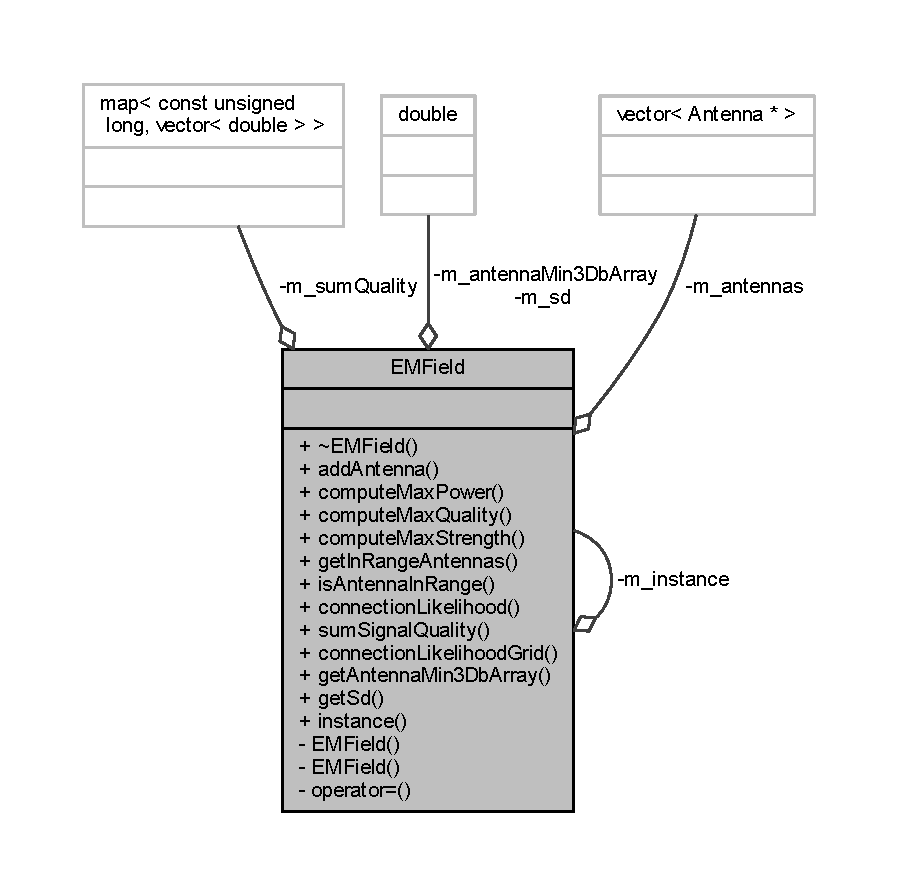
\includegraphics[width=350pt]{class_e_m_field__coll__graph}
\end{center}
\end{figure}
\subsection*{Public Member Functions}
\begin{DoxyCompactItemize}
\item 
virtual \mbox{\hyperlink{class_e_m_field_abe7db07a27a120858107d5efa5f14edb}{$\sim$\+E\+M\+Field}} ()
\item 
void \mbox{\hyperlink{class_e_m_field_ac531ecbce4c81aa5da19fe3c734a585c}{add\+Antenna}} (\mbox{\hyperlink{class_antenna}{Antenna}} $\ast$a)
\item 
pair$<$ \mbox{\hyperlink{class_antenna}{Antenna}} $\ast$, double $>$ \mbox{\hyperlink{class_e_m_field_a01cfb9fea3dadfcfe5d6f00551193acd}{compute\+Max\+Power}} (const Point $\ast$p, const unsigned long mno\+Id)
\item 
pair$<$ \mbox{\hyperlink{class_antenna}{Antenna}} $\ast$, double $>$ \mbox{\hyperlink{class_e_m_field_ac866f6224e34895a0ee085c4baf43a01}{compute\+Max\+Quality}} (const Point $\ast$p, const unsigned long mno\+Id)
\item 
pair$<$ \mbox{\hyperlink{class_antenna}{Antenna}} $\ast$, double $>$ \mbox{\hyperlink{class_e_m_field_a9a3cdbca4fcf408ce58a30fb98de1bbb}{compute\+Max\+Strength}} (const Point $\ast$p, const unsigned long mno\+Id)
\item 
vector$<$ pair$<$ \mbox{\hyperlink{class_antenna}{Antenna}} $\ast$, double $>$ $>$ \mbox{\hyperlink{class_e_m_field_a2ad800417b06a62e68edd1fccb5c4b93}{get\+In\+Range\+Antennas}} (const Point $\ast$p, const double threshold, const \mbox{\hyperlink{class_holdable_agent_ae2c334b004d7b9c5a999cf2618e4e518}{Holdable\+Agent\+::\+C\+O\+N\+N\+E\+C\+T\+I\+O\+N\+\_\+\+T\+Y\+PE}} conn\+Type, unsigned long mno\+Id)
\item 
bool \mbox{\hyperlink{class_e_m_field_a5cd43aded41779d2d24de3f3e5c717d0}{is\+Antenna\+In\+Range}} (const Point $\ast$p, \mbox{\hyperlink{class_antenna}{Antenna}} $\ast$a, const double threshold, const \mbox{\hyperlink{class_holdable_agent_ae2c334b004d7b9c5a999cf2618e4e518}{Holdable\+Agent\+::\+C\+O\+N\+N\+E\+C\+T\+I\+O\+N\+\_\+\+T\+Y\+PE}} conn\+Type)
\item 
double \mbox{\hyperlink{class_e_m_field_a710da64db53718cdeed7b8c8dc11bba3}{connection\+Likelihood}} (\mbox{\hyperlink{class_antenna}{Antenna}} $\ast$a, const Point $\ast$p)
\item 
vector$<$ double $>$ \mbox{\hyperlink{class_e_m_field_a4995bf4b93c09f12b7aab64c7eb24603}{sum\+Signal\+Quality}} (const \mbox{\hyperlink{class_grid}{Grid}} $\ast$grid, const unsigned long mno\+ID)
\item 
double \mbox{\hyperlink{class_e_m_field_a533effeee35a80746ea7e3ddc5998e48}{connection\+Likelihood\+Grid}} (\mbox{\hyperlink{class_antenna}{Antenna}} $\ast$a, const \mbox{\hyperlink{class_grid}{Grid}} $\ast$g, unsigned long tile\+Index)
\item 
const double $\ast$ \mbox{\hyperlink{class_e_m_field_ab2132484b9c52f2224bc81f354b24df6}{get\+Antenna\+Min3\+Db\+Array}} () const
\item 
double $\ast$ \mbox{\hyperlink{class_e_m_field_a0fea003948a67df01174480480376169}{get\+Sd}} () const
\end{DoxyCompactItemize}
\subsection*{Static Public Member Functions}
\begin{DoxyCompactItemize}
\item 
static \mbox{\hyperlink{class_e_m_field}{E\+M\+Field}} $\ast$ \mbox{\hyperlink{class_e_m_field_acbadbede116ac320398cbfcd19e90ec7}{instance}} ()
\end{DoxyCompactItemize}
\subsection*{Private Member Functions}
\begin{DoxyCompactItemize}
\item 
\mbox{\hyperlink{class_e_m_field_a054f389cfa853008f32c02d874aa4d58}{E\+M\+Field}} ()
\item 
\mbox{\hyperlink{class_e_m_field_a7760631ded36ba2c5a918c97a1cc93e9}{E\+M\+Field}} (const \mbox{\hyperlink{class_e_m_field}{E\+M\+Field}} \&)
\item 
\mbox{\hyperlink{class_e_m_field}{E\+M\+Field}} \& \mbox{\hyperlink{class_e_m_field_ad35e4754cad2016d7df1b8ac45540b35}{operator=}} (const \mbox{\hyperlink{class_e_m_field}{E\+M\+Field}} \&)
\end{DoxyCompactItemize}
\subsection*{Private Attributes}
\begin{DoxyCompactItemize}
\item 
vector$<$ \mbox{\hyperlink{class_antenna}{Antenna}} $\ast$ $>$ \mbox{\hyperlink{class_e_m_field_ab74a3bde70b66fd033bde6c25345a755}{m\+\_\+antennas}}
\item 
map$<$ const unsigned long, vector$<$ double $>$ $>$ \mbox{\hyperlink{class_e_m_field_a18e5a4d972d888c5da458e30e426c7ae}{m\+\_\+sum\+Quality}}
\item 
double $\ast$ \mbox{\hyperlink{class_e_m_field_a96c4c7bc39c2f8afea0dca3280fe145c}{m\+\_\+antenna\+Min3\+Db\+Array}}
\item 
double $\ast$ \mbox{\hyperlink{class_e_m_field_ac2142eafd5b82e43437a8047565f619c}{m\+\_\+sd}}
\end{DoxyCompactItemize}
\subsection*{Static Private Attributes}
\begin{DoxyCompactItemize}
\item 
static \mbox{\hyperlink{class_e_m_field}{E\+M\+Field}} $\ast$ \mbox{\hyperlink{class_e_m_field_a3a75e412fa15cfab78ce64dfbb8af52d}{m\+\_\+instance}}
\end{DoxyCompactItemize}


\subsection{Detailed Description}
This utility singleton class is used to compute different measures of the electromagnetic field radiated by an antenna (power, signal strength etc) and it also provides methods needed to decide to which antenna a mobile device connects. 

\subsection{Constructor \& Destructor Documentation}
\mbox{\Hypertarget{class_e_m_field_abe7db07a27a120858107d5efa5f14edb}\label{class_e_m_field_abe7db07a27a120858107d5efa5f14edb}} 
\index{EMField@{EMField}!````~EMField@{$\sim$EMField}}
\index{````~EMField@{$\sim$EMField}!EMField@{EMField}}
\subsubsection{\texorpdfstring{$\sim$EMField()}{~EMField()}}
{\footnotesize\ttfamily virtual E\+M\+Field\+::$\sim$\+E\+M\+Field (\begin{DoxyParamCaption}{ }\end{DoxyParamCaption})\hspace{0.3cm}{\ttfamily [virtual]}}

Default destructor. \mbox{\Hypertarget{class_e_m_field_a054f389cfa853008f32c02d874aa4d58}\label{class_e_m_field_a054f389cfa853008f32c02d874aa4d58}} 
\index{EMField@{EMField}!EMField@{EMField}}
\index{EMField@{EMField}!EMField@{EMField}}
\subsubsection{\texorpdfstring{EMField()}{EMField()}\hspace{0.1cm}{\footnotesize\ttfamily [1/2]}}
{\footnotesize\ttfamily E\+M\+Field\+::\+E\+M\+Field (\begin{DoxyParamCaption}{ }\end{DoxyParamCaption})\hspace{0.3cm}{\ttfamily [private]}}

\mbox{\Hypertarget{class_e_m_field_a7760631ded36ba2c5a918c97a1cc93e9}\label{class_e_m_field_a7760631ded36ba2c5a918c97a1cc93e9}} 
\index{EMField@{EMField}!EMField@{EMField}}
\index{EMField@{EMField}!EMField@{EMField}}
\subsubsection{\texorpdfstring{EMField()}{EMField()}\hspace{0.1cm}{\footnotesize\ttfamily [2/2]}}
{\footnotesize\ttfamily E\+M\+Field\+::\+E\+M\+Field (\begin{DoxyParamCaption}\item[{const \mbox{\hyperlink{class_e_m_field}{E\+M\+Field}} \&}]{ }\end{DoxyParamCaption})\hspace{0.3cm}{\ttfamily [private]}}



\subsection{Member Function Documentation}
\mbox{\Hypertarget{class_e_m_field_ac531ecbce4c81aa5da19fe3c734a585c}\label{class_e_m_field_ac531ecbce4c81aa5da19fe3c734a585c}} 
\index{EMField@{EMField}!addAntenna@{addAntenna}}
\index{addAntenna@{addAntenna}!EMField@{EMField}}
\subsubsection{\texorpdfstring{addAntenna()}{addAntenna()}}
{\footnotesize\ttfamily void E\+M\+Field\+::add\+Antenna (\begin{DoxyParamCaption}\item[{\mbox{\hyperlink{class_antenna}{Antenna}} $\ast$}]{a }\end{DoxyParamCaption})}

Add a pointer to an \mbox{\hyperlink{class_antenna}{Antenna}} object to an internal collection needed for computations. Although these pointers are kept in an Agent\+Collection object they are also added to a local vector in this class for performance reasons. 
\begin{DoxyParams}{Parameters}
{\em a} & a pointer to the \mbox{\hyperlink{class_antenna}{Antenna}} object \\
\hline
\end{DoxyParams}
\mbox{\Hypertarget{class_e_m_field_a01cfb9fea3dadfcfe5d6f00551193acd}\label{class_e_m_field_a01cfb9fea3dadfcfe5d6f00551193acd}} 
\index{EMField@{EMField}!computeMaxPower@{computeMaxPower}}
\index{computeMaxPower@{computeMaxPower}!EMField@{EMField}}
\subsubsection{\texorpdfstring{computeMaxPower()}{computeMaxPower()}}
{\footnotesize\ttfamily pair$<$\mbox{\hyperlink{class_antenna}{Antenna}}$\ast$, double$>$ E\+M\+Field\+::compute\+Max\+Power (\begin{DoxyParamCaption}\item[{const Point $\ast$}]{p,  }\item[{const unsigned long}]{mno\+Id }\end{DoxyParamCaption})}

Returns a pair made of a pointer to an \mbox{\hyperlink{class_antenna}{Antenna}} object and its power with the property that in the location specified by parameter p, the \mbox{\hyperlink{class_antenna}{Antenna}} returned by this method provides the highest power (the power of the field is considered to decrease according a power-\/law). 
\begin{DoxyParams}{Parameters}
{\em p} & the location where we want to find which \mbox{\hyperlink{class_antenna}{Antenna}} provides the highest power the of electromagnetic field. \\
\hline
{\em mno\+Id} & the id of the M\+NO for which we compute the power. Only antennas belonging to this M\+NO will be considered during computations. \\
\hline
\end{DoxyParams}
\begin{DoxyReturn}{Returns}
a pair$<$\+Antenna$\ast$, double$>$ containing a pointer to the \mbox{\hyperlink{class_antenna}{Antenna}} object that provides the highest power of the field in the location specified by p. 
\end{DoxyReturn}
\mbox{\Hypertarget{class_e_m_field_ac866f6224e34895a0ee085c4baf43a01}\label{class_e_m_field_ac866f6224e34895a0ee085c4baf43a01}} 
\index{EMField@{EMField}!computeMaxQuality@{computeMaxQuality}}
\index{computeMaxQuality@{computeMaxQuality}!EMField@{EMField}}
\subsubsection{\texorpdfstring{computeMaxQuality()}{computeMaxQuality()}}
{\footnotesize\ttfamily pair$<$\mbox{\hyperlink{class_antenna}{Antenna}}$\ast$, double$>$ E\+M\+Field\+::compute\+Max\+Quality (\begin{DoxyParamCaption}\item[{const Point $\ast$}]{p,  }\item[{const unsigned long}]{mno\+Id }\end{DoxyParamCaption})}

Returns a pair made of a pointer to an \mbox{\hyperlink{class_antenna}{Antenna}} object and its signal quality with the property that in the location specified by p, the \mbox{\hyperlink{class_antenna}{Antenna}} returned by this method provides signal with the highest quality. The signal quality in this pair is the computed in location given by p. 
\begin{DoxyParams}{Parameters}
{\em p} & indicates the location where we want to find which \mbox{\hyperlink{class_antenna}{Antenna}} provides the highest quality of the signal. \\
\hline
{\em mno\+Id} & the id of the M\+NO for which we compute the signal quality. Only antennas belonging to this M\+NO will be considered during computations. \\
\hline
\end{DoxyParams}
\begin{DoxyReturn}{Returns}
a pair$<$\+Antenna$\ast$, double$>$ containing a pointer to the \mbox{\hyperlink{class_antenna}{Antenna}} object that provides a signal with the highest quality in location given by p. 
\end{DoxyReturn}
\mbox{\Hypertarget{class_e_m_field_a9a3cdbca4fcf408ce58a30fb98de1bbb}\label{class_e_m_field_a9a3cdbca4fcf408ce58a30fb98de1bbb}} 
\index{EMField@{EMField}!computeMaxStrength@{computeMaxStrength}}
\index{computeMaxStrength@{computeMaxStrength}!EMField@{EMField}}
\subsubsection{\texorpdfstring{computeMaxStrength()}{computeMaxStrength()}}
{\footnotesize\ttfamily pair$<$\mbox{\hyperlink{class_antenna}{Antenna}}$\ast$, double$>$ E\+M\+Field\+::compute\+Max\+Strength (\begin{DoxyParamCaption}\item[{const Point $\ast$}]{p,  }\item[{const unsigned long}]{mno\+Id }\end{DoxyParamCaption})}

Returns a pair made of a pointer to an \mbox{\hyperlink{class_antenna}{Antenna}} object and its signal strength with the property that in the location specified by p, the \mbox{\hyperlink{class_antenna}{Antenna}} returned by this method provides signal with the highest strength. The signal strength in this pair is the computed in location given by p. 
\begin{DoxyParams}{Parameters}
{\em p} & indicates the location where we want to find which \mbox{\hyperlink{class_antenna}{Antenna}} provides the highest strength of the signal. \\
\hline
{\em mno\+Id} & the id of the M\+NO for which we compute the signal strength. Only antennas belonging to this M\+NO will be considered during computations. \\
\hline
\end{DoxyParams}
\begin{DoxyReturn}{Returns}
a pair$<$\+Antenna$\ast$, double$>$ containing a pointer to the \mbox{\hyperlink{class_antenna}{Antenna}} object that provides a signal with the highest strength in location given by p. 
\end{DoxyReturn}
\mbox{\Hypertarget{class_e_m_field_a710da64db53718cdeed7b8c8dc11bba3}\label{class_e_m_field_a710da64db53718cdeed7b8c8dc11bba3}} 
\index{EMField@{EMField}!connectionLikelihood@{connectionLikelihood}}
\index{connectionLikelihood@{connectionLikelihood}!EMField@{EMField}}
\subsubsection{\texorpdfstring{connectionLikelihood()}{connectionLikelihood()}}
{\footnotesize\ttfamily double E\+M\+Field\+::connection\+Likelihood (\begin{DoxyParamCaption}\item[{\mbox{\hyperlink{class_antenna}{Antenna}} $\ast$}]{a,  }\item[{const Point $\ast$}]{p }\end{DoxyParamCaption})}

Computes the connection likelihood for \mbox{\hyperlink{class_antenna}{Antenna}} indicated by a in a certain location given by p. The connection likelihood is computed dividing the signal quality provided by \mbox{\hyperlink{class_antenna}{Antenna}} indicated through p by the sum of the signal quality provided by all antennas of an M\+NO. 
\begin{DoxyParams}{Parameters}
{\em a} & a pointer to an \mbox{\hyperlink{class_antenna}{Antenna}} object. \\
\hline
{\em p} & a location in space. \\
\hline
\end{DoxyParams}
\begin{DoxyReturn}{Returns}
the connection likelihood for \mbox{\hyperlink{class_antenna}{Antenna}} a in location p. 
\end{DoxyReturn}
\mbox{\Hypertarget{class_e_m_field_a533effeee35a80746ea7e3ddc5998e48}\label{class_e_m_field_a533effeee35a80746ea7e3ddc5998e48}} 
\index{EMField@{EMField}!connectionLikelihoodGrid@{connectionLikelihoodGrid}}
\index{connectionLikelihoodGrid@{connectionLikelihoodGrid}!EMField@{EMField}}
\subsubsection{\texorpdfstring{connectionLikelihoodGrid()}{connectionLikelihoodGrid()}}
{\footnotesize\ttfamily double E\+M\+Field\+::connection\+Likelihood\+Grid (\begin{DoxyParamCaption}\item[{\mbox{\hyperlink{class_antenna}{Antenna}} $\ast$}]{a,  }\item[{const \mbox{\hyperlink{class_grid}{Grid}} $\ast$}]{g,  }\item[{unsigned long}]{tile\+Index }\end{DoxyParamCaption})}

Computes the connection likelihood for \mbox{\hyperlink{class_antenna}{Antenna}} indicated by a in the center of the tile indicated by tile\+Index 
\begin{DoxyParams}{Parameters}
{\em a} & a pointer to an \mbox{\hyperlink{class_antenna}{Antenna}} object. \\
\hline
{\em g} & a pointer to the reference \mbox{\hyperlink{class_grid}{Grid}} object \\
\hline
{\em tile\+Index} & the index of the tile where we want to compute the connection likelihood. \\
\hline
\end{DoxyParams}
\begin{DoxyReturn}{Returns}
the connection likelihood for \mbox{\hyperlink{class_antenna}{Antenna}} a in the center of the tile with the index tile\+Index. 
\end{DoxyReturn}
\mbox{\Hypertarget{class_e_m_field_ab2132484b9c52f2224bc81f354b24df6}\label{class_e_m_field_ab2132484b9c52f2224bc81f354b24df6}} 
\index{EMField@{EMField}!getAntennaMin3DbArray@{getAntennaMin3DbArray}}
\index{getAntennaMin3DbArray@{getAntennaMin3DbArray}!EMField@{EMField}}
\subsubsection{\texorpdfstring{getAntennaMin3DbArray()}{getAntennaMin3DbArray()}}
{\footnotesize\ttfamily const double$\ast$ E\+M\+Field\+::get\+Antenna\+Min3\+Db\+Array (\begin{DoxyParamCaption}{ }\end{DoxyParamCaption}) const}

\mbox{\Hypertarget{class_e_m_field_a2ad800417b06a62e68edd1fccb5c4b93}\label{class_e_m_field_a2ad800417b06a62e68edd1fccb5c4b93}} 
\index{EMField@{EMField}!getInRangeAntennas@{getInRangeAntennas}}
\index{getInRangeAntennas@{getInRangeAntennas}!EMField@{EMField}}
\subsubsection{\texorpdfstring{getInRangeAntennas()}{getInRangeAntennas()}}
{\footnotesize\ttfamily vector$<$pair$<$\mbox{\hyperlink{class_antenna}{Antenna}}$\ast$, double$>$ $>$ E\+M\+Field\+::get\+In\+Range\+Antennas (\begin{DoxyParamCaption}\item[{const Point $\ast$}]{p,  }\item[{const double}]{threshold,  }\item[{const \mbox{\hyperlink{class_holdable_agent_ae2c334b004d7b9c5a999cf2618e4e518}{Holdable\+Agent\+::\+C\+O\+N\+N\+E\+C\+T\+I\+O\+N\+\_\+\+T\+Y\+PE}}}]{conn\+Type,  }\item[{unsigned long}]{mno\+Id }\end{DoxyParamCaption})}

Returns a vector of pairs made up of a pointer to an \mbox{\hyperlink{class_antenna}{Antenna}} object and its power, signal quality or signal strength. All the antennas in this vector provides a signal with a power or signal quality greater than the threshold provided as threshold, i.\+e. this vector contains all antennas that have in their coverage area the location given by point p. 
\begin{DoxyParams}{Parameters}
{\em p} & the location where we want to have the list with the all antennas that covers it. \\
\hline
{\em threshold} & the lowest limit of the power or signal quality below which the signal is considered to be only noise, i.\+e. it defines the limit of the coverage area. \\
\hline
{\em conn\+Type} & indicates the mechanism used to set up a connection between an antenna and a mobile phone \\
\hline
{\em mno\+Id} & the id of the M\+NO for which we build the resulting vector. Only antennas belonging to this M\+NO will be considered during computations. \\
\hline
\end{DoxyParams}
\begin{DoxyReturn}{Returns}
a vector of pairs made up of a pointer to an \mbox{\hyperlink{class_antenna}{Antenna}} object and its power, signal quality or signal strength, according to the value of the conn\+Type. All the antennas in this vector provides a signal with a power, signal quality or signal strength greater than the threshold. 
\end{DoxyReturn}
\mbox{\Hypertarget{class_e_m_field_a0fea003948a67df01174480480376169}\label{class_e_m_field_a0fea003948a67df01174480480376169}} 
\index{EMField@{EMField}!getSd@{getSd}}
\index{getSd@{getSd}!EMField@{EMField}}
\subsubsection{\texorpdfstring{getSd()}{getSd()}}
{\footnotesize\ttfamily double$\ast$ E\+M\+Field\+::get\+Sd (\begin{DoxyParamCaption}{ }\end{DoxyParamCaption}) const}

\mbox{\Hypertarget{class_e_m_field_acbadbede116ac320398cbfcd19e90ec7}\label{class_e_m_field_acbadbede116ac320398cbfcd19e90ec7}} 
\index{EMField@{EMField}!instance@{instance}}
\index{instance@{instance}!EMField@{EMField}}
\subsubsection{\texorpdfstring{instance()}{instance()}}
{\footnotesize\ttfamily static \mbox{\hyperlink{class_e_m_field}{E\+M\+Field}}$\ast$ E\+M\+Field\+::instance (\begin{DoxyParamCaption}{ }\end{DoxyParamCaption})\hspace{0.3cm}{\ttfamily [inline]}, {\ttfamily [static]}}

Returns an instance of this class. This class is a singleton. \begin{DoxyReturn}{Returns}
an instance of this class. 
\end{DoxyReturn}
\mbox{\Hypertarget{class_e_m_field_a5cd43aded41779d2d24de3f3e5c717d0}\label{class_e_m_field_a5cd43aded41779d2d24de3f3e5c717d0}} 
\index{EMField@{EMField}!isAntennaInRange@{isAntennaInRange}}
\index{isAntennaInRange@{isAntennaInRange}!EMField@{EMField}}
\subsubsection{\texorpdfstring{isAntennaInRange()}{isAntennaInRange()}}
{\footnotesize\ttfamily bool E\+M\+Field\+::is\+Antenna\+In\+Range (\begin{DoxyParamCaption}\item[{const Point $\ast$}]{p,  }\item[{\mbox{\hyperlink{class_antenna}{Antenna}} $\ast$}]{a,  }\item[{const double}]{threshold,  }\item[{const \mbox{\hyperlink{class_holdable_agent_ae2c334b004d7b9c5a999cf2618e4e518}{Holdable\+Agent\+::\+C\+O\+N\+N\+E\+C\+T\+I\+O\+N\+\_\+\+T\+Y\+PE}}}]{conn\+Type }\end{DoxyParamCaption})}

Checks if p is in the coverage area of \mbox{\hyperlink{class_antenna}{Antenna}} pointed out by a. The coverage area is considered the area where the signal quality or the power of the field is greater than the value of threshold. 
\begin{DoxyParams}{Parameters}
{\em p} & the location that we want to check the power or the quality of the signal \\
\hline
{\em a} & pointer to an \mbox{\hyperlink{class_antenna}{Antenna}} object for which we want to check if it covers the point p. \\
\hline
{\em threshold} & the lower limit of the power or signal quality below which the signal is considered only noise. \\
\hline
{\em conn\+Type} & indicates the mechanism used to set up a connection between an antenna and a mobile phone. \\
\hline
\end{DoxyParams}
\begin{DoxyReturn}{Returns}
true is the \mbox{\hyperlink{class_antenna}{Antenna}} object provide enough power or signal quality in the location given as p. 
\end{DoxyReturn}
\mbox{\Hypertarget{class_e_m_field_ad35e4754cad2016d7df1b8ac45540b35}\label{class_e_m_field_ad35e4754cad2016d7df1b8ac45540b35}} 
\index{EMField@{EMField}!operator=@{operator=}}
\index{operator=@{operator=}!EMField@{EMField}}
\subsubsection{\texorpdfstring{operator=()}{operator=()}}
{\footnotesize\ttfamily \mbox{\hyperlink{class_e_m_field}{E\+M\+Field}}\& E\+M\+Field\+::operator= (\begin{DoxyParamCaption}\item[{const \mbox{\hyperlink{class_e_m_field}{E\+M\+Field}} \&}]{ }\end{DoxyParamCaption})\hspace{0.3cm}{\ttfamily [private]}}

\mbox{\Hypertarget{class_e_m_field_a4995bf4b93c09f12b7aab64c7eb24603}\label{class_e_m_field_a4995bf4b93c09f12b7aab64c7eb24603}} 
\index{EMField@{EMField}!sumSignalQuality@{sumSignalQuality}}
\index{sumSignalQuality@{sumSignalQuality}!EMField@{EMField}}
\subsubsection{\texorpdfstring{sumSignalQuality()}{sumSignalQuality()}}
{\footnotesize\ttfamily vector$<$double$>$ E\+M\+Field\+::sum\+Signal\+Quality (\begin{DoxyParamCaption}\item[{const \mbox{\hyperlink{class_grid}{Grid}} $\ast$}]{grid,  }\item[{const unsigned long}]{mno\+ID }\end{DoxyParamCaption})}

Computes the sum of the signal quality given by all antennas belonging to an M\+NO for all tiles in the reference grid. The signal quality is computed in the center of each tile. 
\begin{DoxyParams}{Parameters}
{\em grid} & the grid of tiles where this method computes the sum of the signal quality. This grid is set at the beginning of the simulation and it overlaps the \mbox{\hyperlink{class_map}{Map}}. \\
\hline
{\em mno\+ID} & the id of the M\+NO for which we want to compute this sum. \\
\hline
\end{DoxyParams}
\begin{DoxyReturn}{Returns}
a vector containing the sum of the signal quality given by all antennas of an M\+NO, for all tiles in the reference grid. An element of the vector corresponds to a tile in the grid. The tiles are linearized in a row-\/major order starting with the bottom-\/left corner. 
\end{DoxyReturn}


\subsection{Member Data Documentation}
\mbox{\Hypertarget{class_e_m_field_a96c4c7bc39c2f8afea0dca3280fe145c}\label{class_e_m_field_a96c4c7bc39c2f8afea0dca3280fe145c}} 
\index{EMField@{EMField}!m\_antennaMin3DbArray@{m\_antennaMin3DbArray}}
\index{m\_antennaMin3DbArray@{m\_antennaMin3DbArray}!EMField@{EMField}}
\subsubsection{\texorpdfstring{m\_antennaMin3DbArray}{m\_antennaMin3DbArray}}
{\footnotesize\ttfamily double$\ast$ E\+M\+Field\+::m\+\_\+antenna\+Min3\+Db\+Array\hspace{0.3cm}{\ttfamily [private]}}

\mbox{\Hypertarget{class_e_m_field_ab74a3bde70b66fd033bde6c25345a755}\label{class_e_m_field_ab74a3bde70b66fd033bde6c25345a755}} 
\index{EMField@{EMField}!m\_antennas@{m\_antennas}}
\index{m\_antennas@{m\_antennas}!EMField@{EMField}}
\subsubsection{\texorpdfstring{m\_antennas}{m\_antennas}}
{\footnotesize\ttfamily vector$<$\mbox{\hyperlink{class_antenna}{Antenna}}$\ast$$>$ E\+M\+Field\+::m\+\_\+antennas\hspace{0.3cm}{\ttfamily [private]}}

\mbox{\Hypertarget{class_e_m_field_a3a75e412fa15cfab78ce64dfbb8af52d}\label{class_e_m_field_a3a75e412fa15cfab78ce64dfbb8af52d}} 
\index{EMField@{EMField}!m\_instance@{m\_instance}}
\index{m\_instance@{m\_instance}!EMField@{EMField}}
\subsubsection{\texorpdfstring{m\_instance}{m\_instance}}
{\footnotesize\ttfamily \mbox{\hyperlink{class_e_m_field}{E\+M\+Field}}$\ast$ E\+M\+Field\+::m\+\_\+instance\hspace{0.3cm}{\ttfamily [static]}, {\ttfamily [private]}}

\mbox{\Hypertarget{class_e_m_field_ac2142eafd5b82e43437a8047565f619c}\label{class_e_m_field_ac2142eafd5b82e43437a8047565f619c}} 
\index{EMField@{EMField}!m\_sd@{m\_sd}}
\index{m\_sd@{m\_sd}!EMField@{EMField}}
\subsubsection{\texorpdfstring{m\_sd}{m\_sd}}
{\footnotesize\ttfamily double$\ast$ E\+M\+Field\+::m\+\_\+sd\hspace{0.3cm}{\ttfamily [private]}}

\mbox{\Hypertarget{class_e_m_field_a18e5a4d972d888c5da458e30e426c7ae}\label{class_e_m_field_a18e5a4d972d888c5da458e30e426c7ae}} 
\index{EMField@{EMField}!m\_sumQuality@{m\_sumQuality}}
\index{m\_sumQuality@{m\_sumQuality}!EMField@{EMField}}
\subsubsection{\texorpdfstring{m\_sumQuality}{m\_sumQuality}}
{\footnotesize\ttfamily map$<$const unsigned long, vector$<$double$>$ $>$ E\+M\+Field\+::m\+\_\+sum\+Quality\hspace{0.3cm}{\ttfamily [private]}}



The documentation for this class was generated from the following file\+:\begin{DoxyCompactItemize}
\item 
include/\mbox{\hyperlink{_e_m_field_8h}{E\+M\+Field.\+h}}\end{DoxyCompactItemize}

\section{tinyxml2\+::Entity Struct Reference}
\label{structtinyxml2_1_1_entity}\index{tinyxml2::Entity@{tinyxml2::Entity}}
\subsection*{Public Attributes}
\begin{DoxyCompactItemize}
\item 
const char $\ast$ \textbf{ pattern}
\item 
int \textbf{ length}
\item 
char \textbf{ value}
\end{DoxyCompactItemize}


\subsection{Detailed Description}


Definition at line 122 of file tinyxml2.\+cpp.



\subsection{Member Data Documentation}
\mbox{\label{structtinyxml2_1_1_entity_a25e2b57cb59cb4fa68f283d7cb570f21}} 
\index{tinyxml2::Entity@{tinyxml2::Entity}!length@{length}}
\index{length@{length}!tinyxml2::Entity@{tinyxml2::Entity}}
\subsubsection{length}
{\footnotesize\ttfamily int tinyxml2\+::\+Entity\+::length}



Definition at line 124 of file tinyxml2.\+cpp.



Referenced by tinyxml2\+::\+Str\+Pair\+::\+Get\+Str().

\mbox{\label{structtinyxml2_1_1_entity_ab330f5d665d29bfc811ecfa76315894b}} 
\index{tinyxml2::Entity@{tinyxml2::Entity}!pattern@{pattern}}
\index{pattern@{pattern}!tinyxml2::Entity@{tinyxml2::Entity}}
\subsubsection{pattern}
{\footnotesize\ttfamily const char$\ast$ tinyxml2\+::\+Entity\+::pattern}



Definition at line 123 of file tinyxml2.\+cpp.



Referenced by tinyxml2\+::\+Str\+Pair\+::\+Get\+Str().

\mbox{\label{structtinyxml2_1_1_entity_a7334e81e33b4615655a403711b24f3ed}} 
\index{tinyxml2::Entity@{tinyxml2::Entity}!value@{value}}
\index{value@{value}!tinyxml2::Entity@{tinyxml2::Entity}}
\subsubsection{value}
{\footnotesize\ttfamily char tinyxml2\+::\+Entity\+::value}



Definition at line 125 of file tinyxml2.\+cpp.



Referenced by tinyxml2\+::\+Str\+Pair\+::\+Get\+Str(), and tinyxml2\+::\+X\+M\+L\+Printer\+::\+X\+M\+L\+Printer().



The documentation for this struct was generated from the following file\+:\begin{DoxyCompactItemize}
\item 
src/\textbf{ tinyxml2.\+cpp}\end{DoxyCompactItemize}

\section{Error Class Reference}
\label{class_error}\index{Error@{Error}}


{\ttfamily \#include $<$C\+S\+Vparser.\+hpp$>$}

Inheritance diagram for Error\+:\begin{figure}[H]
\begin{center}
\leavevmode
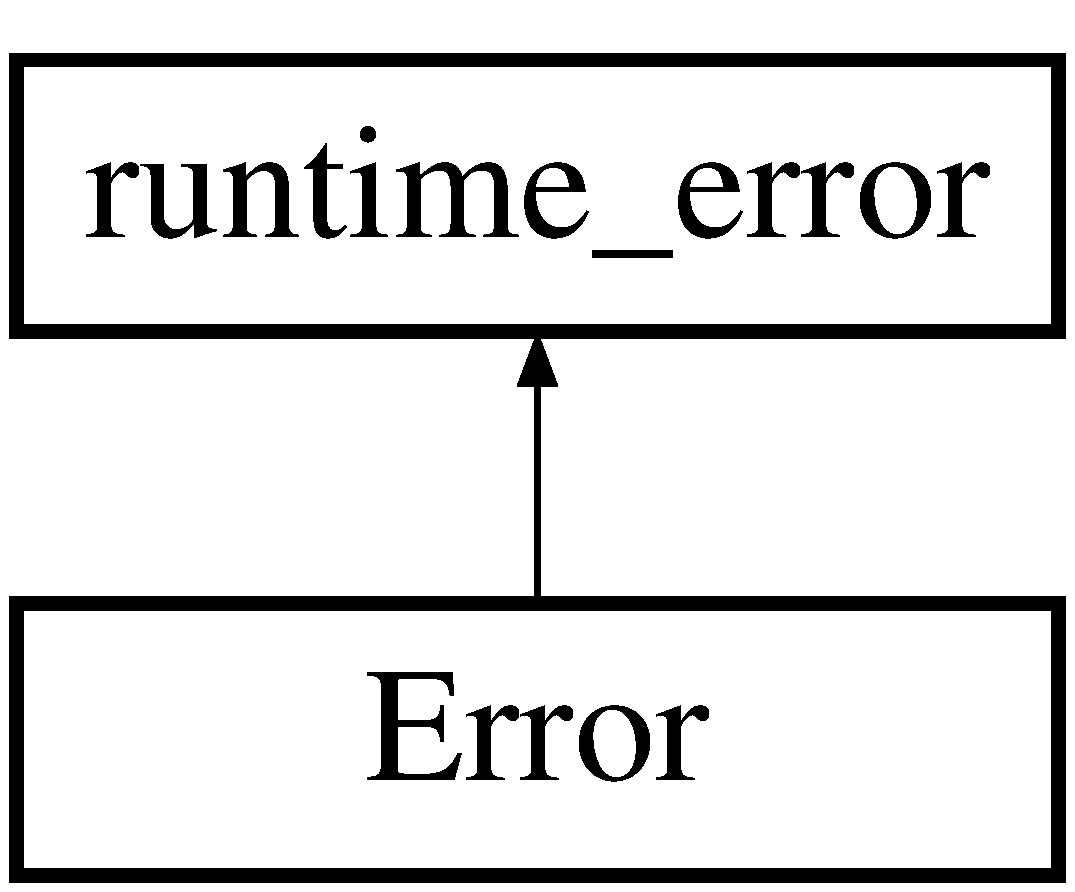
\includegraphics[height=3.000000cm]{class_error}
\end{center}
\end{figure}
\subsection*{Public Member Functions}
\begin{DoxyCompactItemize}
\item 
\textbf{ Error} (const string \&msg)
\end{DoxyCompactItemize}


\subsection{Detailed Description}
This class extends the runtime\+\_\+error class adding an error message 

Definition at line 24 of file C\+S\+Vparser.\+hpp.



\subsection{Constructor \& Destructor Documentation}
\mbox{\label{class_error_af330fc77babbadebc9a12b3aabfe146f}} 
\index{Error@{Error}!Error@{Error}}
\index{Error@{Error}!Error@{Error}}
\subsubsection{Error()}
{\footnotesize\ttfamily Error\+::\+Error (\begin{DoxyParamCaption}\item[{const string \&}]{msg }\end{DoxyParamCaption})\hspace{0.3cm}{\ttfamily [inline]}}

Constructor of the class. 
\begin{DoxyParams}{Parameters}
{\em msg} & the error message \\
\hline
\end{DoxyParams}


Definition at line 31 of file C\+S\+Vparser.\+hpp.



The documentation for this class was generated from the following file\+:\begin{DoxyCompactItemize}
\item 
include/\textbf{ C\+S\+Vparser.\+hpp}\end{DoxyCompactItemize}

\hypertarget{class_grid}{}\section{Grid Class Reference}
\label{class_grid}\index{Grid@{Grid}}


{\ttfamily \#include $<$Grid.\+h$>$}



Collaboration diagram for Grid\+:
\nopagebreak
\begin{figure}[H]
\begin{center}
\leavevmode
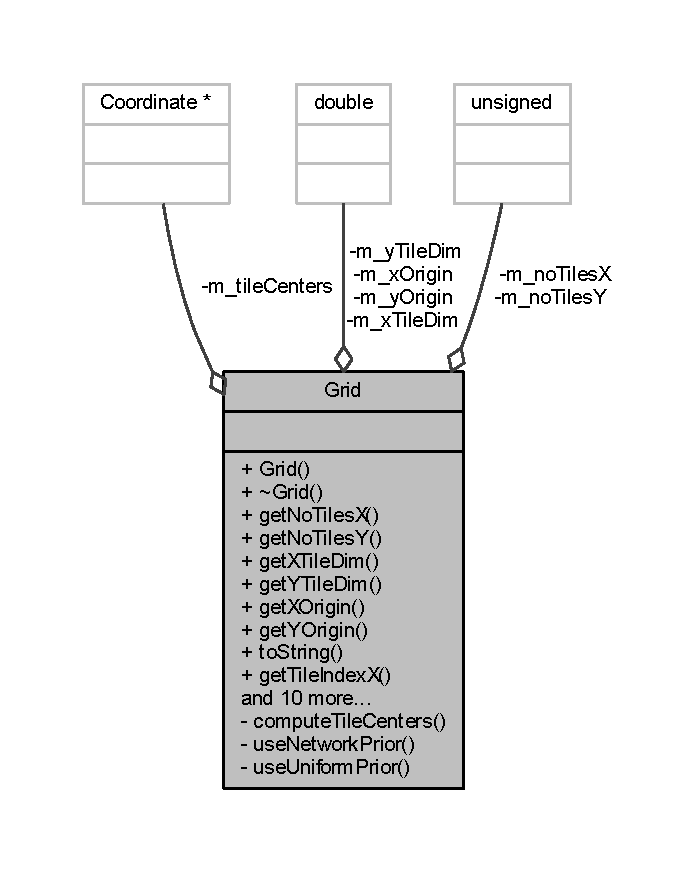
\includegraphics[width=332pt]{class_grid__coll__graph}
\end{center}
\end{figure}
\subsection*{Public Member Functions}
\begin{DoxyCompactItemize}
\item 
\hyperlink{class_grid_a84b0dc169028f21175a4549afde86153}{Grid} (double x\+Orig, double y\+Orig, double x\+Tiledim, double y\+Tiledim, unsigned long no\+TilesX, unsigned long no\+TilesY)
\item 
virtual \hyperlink{class_grid_a241c623291936ddbf4f670a796523a91}{$\sim$\+Grid} ()
\item 
unsigned long \hyperlink{class_grid_af29c0c404a908aa46f83afb17d7609a6}{get\+No\+TilesX} () const
\item 
unsigned long \hyperlink{class_grid_a783a3153d03154cfd33e6a418bb8d390}{get\+No\+TilesY} () const
\item 
double \hyperlink{class_grid_a1c5b9ad91fac264bcdd67f99bc93f663}{get\+X\+Tile\+Dim} () const
\item 
double \hyperlink{class_grid_aedfe477f5be79a375bd64a4d21765918}{get\+Y\+Tile\+Dim} () const
\item 
double \hyperlink{class_grid_a08b534c7f8e1099a6903bf08d9727842}{get\+X\+Origin} () const
\item 
double \hyperlink{class_grid_a53141770920cf261579cf164a8909af9}{get\+Y\+Origin} () const
\item 
const unsigned long \hyperlink{class_grid_ab0a71c762b6c33e6fa2fd49dde38228b}{get\+No\+Tiles} () const
\item 
Coordinate \hyperlink{class_grid_aa8d3de015a2b22d0cd0d72b3e7c29088}{get\+Tile\+Center} (unsigned long tile\+Index) const
\item 
unsigned long \hyperlink{class_grid_a93e42713b7af1f188ce90f92a5e202ab}{get\+Tile\+No} (const Point $\ast$p) const
\item 
unsigned long \hyperlink{class_grid_a02dee9ad3ee575623916c0041f72eb5e}{get\+Tile\+No} (double x, double y) const
\item 
void \hyperlink{class_grid_a0024d8d3cdd7b95f9fd61205ce8b9dea}{dump\+Grid} (const string \&grid\+File\+Name) const
\item 
Coordinate $\ast$ \hyperlink{class_grid_aa1b1f4c938207b16694a27cb9beb66eb}{get\+Tile\+Centers} () const
\end{DoxyCompactItemize}
\subsection*{Private Member Functions}
\begin{DoxyCompactItemize}
\item 
unsigned long \hyperlink{class_grid_a5ab67c336ac08c690a0e8b03c12f02e5}{get\+Tile\+IndexX} (double x) const
\item 
unsigned long \hyperlink{class_grid_ad745f856bb2b27382118ac03fafc06b4}{get\+Tile\+IndexY} (double y) const
\item 
unsigned long \hyperlink{class_grid_af4094832e2adedbbd47889973f5a40da}{get\+Tile\+IndexX} (const Point $\ast$p) const
\item 
unsigned long \hyperlink{class_grid_ae1eeb3b42007ae1cf19cfaf0d846fb9a}{get\+Tile\+IndexY} (const Point $\ast$p) const
\item 
string \hyperlink{class_grid_ad48d195b5e333a94a3a14d6395252b2a}{to\+String} () const
\item 
Coordinate $\ast$ \hyperlink{class_grid_a8948d61db8ba1bda2260590677eaaa01}{compute\+Tile\+Centers} ()
\end{DoxyCompactItemize}
\subsection*{Private Attributes}
\begin{DoxyCompactItemize}
\item 
double \hyperlink{class_grid_ae109d428ac5489815748e92fdde1b91f}{m\+\_\+x\+Origin}
\item 
double \hyperlink{class_grid_a16b2fc5a6e96ad2d59d59b52db83f4aa}{m\+\_\+y\+Origin}
\item 
double \hyperlink{class_grid_a48c3d1fc34a14bff8b9176558a8b6f4e}{m\+\_\+x\+Tile\+Dim}
\item 
double \hyperlink{class_grid_a497eeffc4a16a021e15ecbc130f4f644}{m\+\_\+y\+Tile\+Dim}
\item 
unsigned long \hyperlink{class_grid_a177bfdc70436c25a1510d1abe19e34c1}{m\+\_\+no\+TilesX}
\item 
unsigned long \hyperlink{class_grid_a8fe14c4781dfd5623922fcc1f9c10130}{m\+\_\+no\+TilesY}
\item 
Coordinate $\ast$ \hyperlink{class_grid_a27b99b13ac7e5bec81f7b8704bc3405a}{m\+\_\+tile\+Centers}
\end{DoxyCompactItemize}


\subsection{Detailed Description}
This class implements a grid of rectangular tiles overlapped on the map of the simulation. This grid is used to compute the \char`\"{}observed\char`\"{} location of a mobile phone. This means that we compute the probability of a mobile device to be in a specific tile of the grid using the data recorded by each antenna during the simulation. A finer grid will give a more accurate location but the computational cost increase when the size of the tiles decrease. The tiles of the grid are indexed starting with 0 for the tile in the bottom left corner of the grid in a row-\/major ordering. The last tile, with the biggest index, is the tile in the upper-\/right corner of the grid. 

\subsection{Constructor \& Destructor Documentation}
\mbox{\Hypertarget{class_grid_a84b0dc169028f21175a4549afde86153}\label{class_grid_a84b0dc169028f21175a4549afde86153}} 
\index{Grid@{Grid}!Grid@{Grid}}
\index{Grid@{Grid}!Grid@{Grid}}
\subsubsection{\texorpdfstring{Grid()}{Grid()}}
{\footnotesize\ttfamily Grid\+::\+Grid (\begin{DoxyParamCaption}\item[{double}]{x\+Orig,  }\item[{double}]{y\+Orig,  }\item[{double}]{x\+Tiledim,  }\item[{double}]{y\+Tiledim,  }\item[{unsigned long}]{no\+TilesX,  }\item[{unsigned long}]{no\+TilesY }\end{DoxyParamCaption})}

Constructor of the class. Build a \hyperlink{class_grid}{Grid} object with the specified parameters. 
\begin{DoxyParams}{Parameters}
{\em x\+Orig} & the x coordinate of the origin of the grid (i.\+e. the x coordinate of the bottom left corner of the grid). \\
\hline
{\em y\+Orig} & the y coordinate of the origin of the grid (i.\+e. the y coordinate of the bottom left corner of the grid). \\
\hline
{\em x\+Tiledim} & the dimension of a tile on X axis. \\
\hline
{\em y\+Tiledim} & the dimension of a tile on Y axis. \\
\hline
{\em no\+TilesX} & the number of tiles on X axis. \\
\hline
{\em no\+TilesY} & the number of tiles on Y axis. \\
\hline
\end{DoxyParams}
\mbox{\Hypertarget{class_grid_a241c623291936ddbf4f670a796523a91}\label{class_grid_a241c623291936ddbf4f670a796523a91}} 
\index{Grid@{Grid}!````~Grid@{$\sim$\+Grid}}
\index{````~Grid@{$\sim$\+Grid}!Grid@{Grid}}
\subsubsection{\texorpdfstring{$\sim$\+Grid()}{~Grid()}}
{\footnotesize\ttfamily virtual Grid\+::$\sim$\+Grid (\begin{DoxyParamCaption}{ }\end{DoxyParamCaption})\hspace{0.3cm}{\ttfamily [virtual]}}

Default destructor. 

\subsection{Member Function Documentation}
\mbox{\Hypertarget{class_grid_a8948d61db8ba1bda2260590677eaaa01}\label{class_grid_a8948d61db8ba1bda2260590677eaaa01}} 
\index{Grid@{Grid}!compute\+Tile\+Centers@{compute\+Tile\+Centers}}
\index{compute\+Tile\+Centers@{compute\+Tile\+Centers}!Grid@{Grid}}
\subsubsection{\texorpdfstring{compute\+Tile\+Centers()}{computeTileCenters()}}
{\footnotesize\ttfamily Coordinate$\ast$ Grid\+::compute\+Tile\+Centers (\begin{DoxyParamCaption}{ }\end{DoxyParamCaption})\hspace{0.3cm}{\ttfamily [private]}}

\mbox{\Hypertarget{class_grid_a0024d8d3cdd7b95f9fd61205ce8b9dea}\label{class_grid_a0024d8d3cdd7b95f9fd61205ce8b9dea}} 
\index{Grid@{Grid}!dump\+Grid@{dump\+Grid}}
\index{dump\+Grid@{dump\+Grid}!Grid@{Grid}}
\subsubsection{\texorpdfstring{dump\+Grid()}{dumpGrid()}}
{\footnotesize\ttfamily void Grid\+::dump\+Grid (\begin{DoxyParamCaption}\item[{const string \&}]{grid\+File\+Name }\end{DoxyParamCaption}) const}

Writes the grid description in a .csv file for later processing. 
\begin{DoxyParams}{Parameters}
{\em grid\+File\+Name} & the name of the output file. \\
\hline
\end{DoxyParams}
\mbox{\Hypertarget{class_grid_ab0a71c762b6c33e6fa2fd49dde38228b}\label{class_grid_ab0a71c762b6c33e6fa2fd49dde38228b}} 
\index{Grid@{Grid}!get\+No\+Tiles@{get\+No\+Tiles}}
\index{get\+No\+Tiles@{get\+No\+Tiles}!Grid@{Grid}}
\subsubsection{\texorpdfstring{get\+No\+Tiles()}{getNoTiles()}}
{\footnotesize\ttfamily const unsigned long Grid\+::get\+No\+Tiles (\begin{DoxyParamCaption}{ }\end{DoxyParamCaption}) const}

Computes the total number of tiles in the grid. \begin{DoxyReturn}{Returns}
the total number of tiles in the grid. 
\end{DoxyReturn}
\mbox{\Hypertarget{class_grid_af29c0c404a908aa46f83afb17d7609a6}\label{class_grid_af29c0c404a908aa46f83afb17d7609a6}} 
\index{Grid@{Grid}!get\+No\+TilesX@{get\+No\+TilesX}}
\index{get\+No\+TilesX@{get\+No\+TilesX}!Grid@{Grid}}
\subsubsection{\texorpdfstring{get\+No\+Tiles\+X()}{getNoTilesX()}}
{\footnotesize\ttfamily unsigned long Grid\+::get\+No\+TilesX (\begin{DoxyParamCaption}{ }\end{DoxyParamCaption}) const}

\begin{DoxyReturn}{Returns}
the number of tiles of the grid on X axis direction. 
\end{DoxyReturn}
\mbox{\Hypertarget{class_grid_a783a3153d03154cfd33e6a418bb8d390}\label{class_grid_a783a3153d03154cfd33e6a418bb8d390}} 
\index{Grid@{Grid}!get\+No\+TilesY@{get\+No\+TilesY}}
\index{get\+No\+TilesY@{get\+No\+TilesY}!Grid@{Grid}}
\subsubsection{\texorpdfstring{get\+No\+Tiles\+Y()}{getNoTilesY()}}
{\footnotesize\ttfamily unsigned long Grid\+::get\+No\+TilesY (\begin{DoxyParamCaption}{ }\end{DoxyParamCaption}) const}

\begin{DoxyReturn}{Returns}
the number of tiles of the grid on Y axis direction. 
\end{DoxyReturn}
\mbox{\Hypertarget{class_grid_aa8d3de015a2b22d0cd0d72b3e7c29088}\label{class_grid_aa8d3de015a2b22d0cd0d72b3e7c29088}} 
\index{Grid@{Grid}!get\+Tile\+Center@{get\+Tile\+Center}}
\index{get\+Tile\+Center@{get\+Tile\+Center}!Grid@{Grid}}
\subsubsection{\texorpdfstring{get\+Tile\+Center()}{getTileCenter()}}
{\footnotesize\ttfamily Coordinate Grid\+::get\+Tile\+Center (\begin{DoxyParamCaption}\item[{unsigned long}]{tile\+Index }\end{DoxyParamCaption}) const}

Computes the coordinates of the tile center given by its index in the grid. 
\begin{DoxyParams}{Parameters}
{\em tile\+Index} & the tile index. \\
\hline
\end{DoxyParams}
\begin{DoxyReturn}{Returns}
the coordinates of the center of the tile. 
\end{DoxyReturn}
\mbox{\Hypertarget{class_grid_aa1b1f4c938207b16694a27cb9beb66eb}\label{class_grid_aa1b1f4c938207b16694a27cb9beb66eb}} 
\index{Grid@{Grid}!get\+Tile\+Centers@{get\+Tile\+Centers}}
\index{get\+Tile\+Centers@{get\+Tile\+Centers}!Grid@{Grid}}
\subsubsection{\texorpdfstring{get\+Tile\+Centers()}{getTileCenters()}}
{\footnotesize\ttfamily Coordinate$\ast$ Grid\+::get\+Tile\+Centers (\begin{DoxyParamCaption}{ }\end{DoxyParamCaption}) const}

Returns a vector containing the coordinates of the tile centers. \begin{DoxyReturn}{Returns}
a vector containing the coordinates of the tile centers. 
\end{DoxyReturn}
\mbox{\Hypertarget{class_grid_a5ab67c336ac08c690a0e8b03c12f02e5}\label{class_grid_a5ab67c336ac08c690a0e8b03c12f02e5}} 
\index{Grid@{Grid}!get\+Tile\+IndexX@{get\+Tile\+IndexX}}
\index{get\+Tile\+IndexX@{get\+Tile\+IndexX}!Grid@{Grid}}
\subsubsection{\texorpdfstring{get\+Tile\+Index\+X()}{getTileIndexX()}\hspace{0.1cm}{\footnotesize\ttfamily [1/2]}}
{\footnotesize\ttfamily unsigned long Grid\+::get\+Tile\+IndexX (\begin{DoxyParamCaption}\item[{double}]{x }\end{DoxyParamCaption}) const\hspace{0.3cm}{\ttfamily [private]}}

\mbox{\Hypertarget{class_grid_af4094832e2adedbbd47889973f5a40da}\label{class_grid_af4094832e2adedbbd47889973f5a40da}} 
\index{Grid@{Grid}!get\+Tile\+IndexX@{get\+Tile\+IndexX}}
\index{get\+Tile\+IndexX@{get\+Tile\+IndexX}!Grid@{Grid}}
\subsubsection{\texorpdfstring{get\+Tile\+Index\+X()}{getTileIndexX()}\hspace{0.1cm}{\footnotesize\ttfamily [2/2]}}
{\footnotesize\ttfamily unsigned long Grid\+::get\+Tile\+IndexX (\begin{DoxyParamCaption}\item[{const Point $\ast$}]{p }\end{DoxyParamCaption}) const\hspace{0.3cm}{\ttfamily [private]}}

Returns the tile index on X axis that contains a given point in space, specified by p. 
\begin{DoxyParams}{Parameters}
{\em p} & a pointer to the point for which we need the tile index. \\
\hline
\end{DoxyParams}
\begin{DoxyReturn}{Returns}
the tile index on X axis that contains the point specified by p, i.\+e. a number between 0 and \hyperlink{class_grid_af29c0c404a908aa46f83afb17d7609a6}{get\+No\+Tiles\+X()} -\/ 1. 
\end{DoxyReturn}
\mbox{\Hypertarget{class_grid_ad745f856bb2b27382118ac03fafc06b4}\label{class_grid_ad745f856bb2b27382118ac03fafc06b4}} 
\index{Grid@{Grid}!get\+Tile\+IndexY@{get\+Tile\+IndexY}}
\index{get\+Tile\+IndexY@{get\+Tile\+IndexY}!Grid@{Grid}}
\subsubsection{\texorpdfstring{get\+Tile\+Index\+Y()}{getTileIndexY()}\hspace{0.1cm}{\footnotesize\ttfamily [1/2]}}
{\footnotesize\ttfamily unsigned long Grid\+::get\+Tile\+IndexY (\begin{DoxyParamCaption}\item[{double}]{y }\end{DoxyParamCaption}) const\hspace{0.3cm}{\ttfamily [private]}}

\mbox{\Hypertarget{class_grid_ae1eeb3b42007ae1cf19cfaf0d846fb9a}\label{class_grid_ae1eeb3b42007ae1cf19cfaf0d846fb9a}} 
\index{Grid@{Grid}!get\+Tile\+IndexY@{get\+Tile\+IndexY}}
\index{get\+Tile\+IndexY@{get\+Tile\+IndexY}!Grid@{Grid}}
\subsubsection{\texorpdfstring{get\+Tile\+Index\+Y()}{getTileIndexY()}\hspace{0.1cm}{\footnotesize\ttfamily [2/2]}}
{\footnotesize\ttfamily unsigned long Grid\+::get\+Tile\+IndexY (\begin{DoxyParamCaption}\item[{const Point $\ast$}]{p }\end{DoxyParamCaption}) const\hspace{0.3cm}{\ttfamily [private]}}

Returns the tile index on Y axis that contains a given point in space, specified by p. 
\begin{DoxyParams}{Parameters}
{\em p} & the point in space for which we need the tile index. \\
\hline
\end{DoxyParams}
\begin{DoxyReturn}{Returns}
the tile index on Y axis that contains the point specified by p, i.\+e. a number between 0 and \hyperlink{class_grid_a783a3153d03154cfd33e6a418bb8d390}{get\+No\+Tiles\+Y()} -\/ 1. 
\end{DoxyReturn}
\mbox{\Hypertarget{class_grid_a93e42713b7af1f188ce90f92a5e202ab}\label{class_grid_a93e42713b7af1f188ce90f92a5e202ab}} 
\index{Grid@{Grid}!get\+Tile\+No@{get\+Tile\+No}}
\index{get\+Tile\+No@{get\+Tile\+No}!Grid@{Grid}}
\subsubsection{\texorpdfstring{get\+Tile\+No()}{getTileNo()}\hspace{0.1cm}{\footnotesize\ttfamily [1/2]}}
{\footnotesize\ttfamily unsigned long Grid\+::get\+Tile\+No (\begin{DoxyParamCaption}\item[{const Point $\ast$}]{p }\end{DoxyParamCaption}) const}

Computes the tile index of the tile that contains the Point indicated by p. 
\begin{DoxyParams}{Parameters}
{\em p} & a pointer to a Point object. \\
\hline
\end{DoxyParams}
\begin{DoxyReturn}{Returns}
the tile index of the tile that contains the Point indicated by p. 
\end{DoxyReturn}
\mbox{\Hypertarget{class_grid_a02dee9ad3ee575623916c0041f72eb5e}\label{class_grid_a02dee9ad3ee575623916c0041f72eb5e}} 
\index{Grid@{Grid}!get\+Tile\+No@{get\+Tile\+No}}
\index{get\+Tile\+No@{get\+Tile\+No}!Grid@{Grid}}
\subsubsection{\texorpdfstring{get\+Tile\+No()}{getTileNo()}\hspace{0.1cm}{\footnotesize\ttfamily [2/2]}}
{\footnotesize\ttfamily unsigned long Grid\+::get\+Tile\+No (\begin{DoxyParamCaption}\item[{double}]{x,  }\item[{double}]{y }\end{DoxyParamCaption}) const}

Computes the tile index of the tile that contains a point with coordinates indicated by x and y. 
\begin{DoxyParams}{Parameters}
{\em x} & x coordinate of a location. \\
\hline
{\em y} & y coordinate of a location. \\
\hline
\end{DoxyParams}
\begin{DoxyReturn}{Returns}
the tile index of the tile that contains a point with coordinates indicated by x and y. 
\end{DoxyReturn}
\mbox{\Hypertarget{class_grid_a08b534c7f8e1099a6903bf08d9727842}\label{class_grid_a08b534c7f8e1099a6903bf08d9727842}} 
\index{Grid@{Grid}!get\+X\+Origin@{get\+X\+Origin}}
\index{get\+X\+Origin@{get\+X\+Origin}!Grid@{Grid}}
\subsubsection{\texorpdfstring{get\+X\+Origin()}{getXOrigin()}}
{\footnotesize\ttfamily double Grid\+::get\+X\+Origin (\begin{DoxyParamCaption}{ }\end{DoxyParamCaption}) const}

\begin{DoxyReturn}{Returns}
the x coordinate of the origin of the grid (i.\+e. the x coordinate of the bottom left corner of the grid). 
\end{DoxyReturn}
\mbox{\Hypertarget{class_grid_a1c5b9ad91fac264bcdd67f99bc93f663}\label{class_grid_a1c5b9ad91fac264bcdd67f99bc93f663}} 
\index{Grid@{Grid}!get\+X\+Tile\+Dim@{get\+X\+Tile\+Dim}}
\index{get\+X\+Tile\+Dim@{get\+X\+Tile\+Dim}!Grid@{Grid}}
\subsubsection{\texorpdfstring{get\+X\+Tile\+Dim()}{getXTileDim()}}
{\footnotesize\ttfamily double Grid\+::get\+X\+Tile\+Dim (\begin{DoxyParamCaption}{ }\end{DoxyParamCaption}) const}

\begin{DoxyReturn}{Returns}
the dimension of a tile on X axis direction. 
\end{DoxyReturn}
\mbox{\Hypertarget{class_grid_a53141770920cf261579cf164a8909af9}\label{class_grid_a53141770920cf261579cf164a8909af9}} 
\index{Grid@{Grid}!get\+Y\+Origin@{get\+Y\+Origin}}
\index{get\+Y\+Origin@{get\+Y\+Origin}!Grid@{Grid}}
\subsubsection{\texorpdfstring{get\+Y\+Origin()}{getYOrigin()}}
{\footnotesize\ttfamily double Grid\+::get\+Y\+Origin (\begin{DoxyParamCaption}{ }\end{DoxyParamCaption}) const}

\begin{DoxyReturn}{Returns}
the y coordinate of the origin of the grid (i.\+e. the y coordinate of the bottom left corner of the grid). 
\end{DoxyReturn}
\mbox{\Hypertarget{class_grid_aedfe477f5be79a375bd64a4d21765918}\label{class_grid_aedfe477f5be79a375bd64a4d21765918}} 
\index{Grid@{Grid}!get\+Y\+Tile\+Dim@{get\+Y\+Tile\+Dim}}
\index{get\+Y\+Tile\+Dim@{get\+Y\+Tile\+Dim}!Grid@{Grid}}
\subsubsection{\texorpdfstring{get\+Y\+Tile\+Dim()}{getYTileDim()}}
{\footnotesize\ttfamily double Grid\+::get\+Y\+Tile\+Dim (\begin{DoxyParamCaption}{ }\end{DoxyParamCaption}) const}

\begin{DoxyReturn}{Returns}
the dimension of a tile on Y axis direction. 
\end{DoxyReturn}
\mbox{\Hypertarget{class_grid_ad48d195b5e333a94a3a14d6395252b2a}\label{class_grid_ad48d195b5e333a94a3a14d6395252b2a}} 
\index{Grid@{Grid}!to\+String@{to\+String}}
\index{to\+String@{to\+String}!Grid@{Grid}}
\subsubsection{\texorpdfstring{to\+String()}{toString()}}
{\footnotesize\ttfamily string Grid\+::to\+String (\begin{DoxyParamCaption}{ }\end{DoxyParamCaption}) const\hspace{0.3cm}{\ttfamily [private]}}

\begin{DoxyReturn}{Returns}
a string representation of an object of type \hyperlink{class_grid}{Grid}. This is useful to write a textual description of the grid in a file for later processing. 
\end{DoxyReturn}


\subsection{Member Data Documentation}
\mbox{\Hypertarget{class_grid_a177bfdc70436c25a1510d1abe19e34c1}\label{class_grid_a177bfdc70436c25a1510d1abe19e34c1}} 
\index{Grid@{Grid}!m\+\_\+no\+TilesX@{m\+\_\+no\+TilesX}}
\index{m\+\_\+no\+TilesX@{m\+\_\+no\+TilesX}!Grid@{Grid}}
\subsubsection{\texorpdfstring{m\+\_\+no\+TilesX}{m\_noTilesX}}
{\footnotesize\ttfamily unsigned long Grid\+::m\+\_\+no\+TilesX\hspace{0.3cm}{\ttfamily [private]}}

\mbox{\Hypertarget{class_grid_a8fe14c4781dfd5623922fcc1f9c10130}\label{class_grid_a8fe14c4781dfd5623922fcc1f9c10130}} 
\index{Grid@{Grid}!m\+\_\+no\+TilesY@{m\+\_\+no\+TilesY}}
\index{m\+\_\+no\+TilesY@{m\+\_\+no\+TilesY}!Grid@{Grid}}
\subsubsection{\texorpdfstring{m\+\_\+no\+TilesY}{m\_noTilesY}}
{\footnotesize\ttfamily unsigned long Grid\+::m\+\_\+no\+TilesY\hspace{0.3cm}{\ttfamily [private]}}

\mbox{\Hypertarget{class_grid_a27b99b13ac7e5bec81f7b8704bc3405a}\label{class_grid_a27b99b13ac7e5bec81f7b8704bc3405a}} 
\index{Grid@{Grid}!m\+\_\+tile\+Centers@{m\+\_\+tile\+Centers}}
\index{m\+\_\+tile\+Centers@{m\+\_\+tile\+Centers}!Grid@{Grid}}
\subsubsection{\texorpdfstring{m\+\_\+tile\+Centers}{m\_tileCenters}}
{\footnotesize\ttfamily Coordinate$\ast$ Grid\+::m\+\_\+tile\+Centers\hspace{0.3cm}{\ttfamily [private]}}

\mbox{\Hypertarget{class_grid_ae109d428ac5489815748e92fdde1b91f}\label{class_grid_ae109d428ac5489815748e92fdde1b91f}} 
\index{Grid@{Grid}!m\+\_\+x\+Origin@{m\+\_\+x\+Origin}}
\index{m\+\_\+x\+Origin@{m\+\_\+x\+Origin}!Grid@{Grid}}
\subsubsection{\texorpdfstring{m\+\_\+x\+Origin}{m\_xOrigin}}
{\footnotesize\ttfamily double Grid\+::m\+\_\+x\+Origin\hspace{0.3cm}{\ttfamily [private]}}

\mbox{\Hypertarget{class_grid_a48c3d1fc34a14bff8b9176558a8b6f4e}\label{class_grid_a48c3d1fc34a14bff8b9176558a8b6f4e}} 
\index{Grid@{Grid}!m\+\_\+x\+Tile\+Dim@{m\+\_\+x\+Tile\+Dim}}
\index{m\+\_\+x\+Tile\+Dim@{m\+\_\+x\+Tile\+Dim}!Grid@{Grid}}
\subsubsection{\texorpdfstring{m\+\_\+x\+Tile\+Dim}{m\_xTileDim}}
{\footnotesize\ttfamily double Grid\+::m\+\_\+x\+Tile\+Dim\hspace{0.3cm}{\ttfamily [private]}}

\mbox{\Hypertarget{class_grid_a16b2fc5a6e96ad2d59d59b52db83f4aa}\label{class_grid_a16b2fc5a6e96ad2d59d59b52db83f4aa}} 
\index{Grid@{Grid}!m\+\_\+y\+Origin@{m\+\_\+y\+Origin}}
\index{m\+\_\+y\+Origin@{m\+\_\+y\+Origin}!Grid@{Grid}}
\subsubsection{\texorpdfstring{m\+\_\+y\+Origin}{m\_yOrigin}}
{\footnotesize\ttfamily double Grid\+::m\+\_\+y\+Origin\hspace{0.3cm}{\ttfamily [private]}}

\mbox{\Hypertarget{class_grid_a497eeffc4a16a021e15ecbc130f4f644}\label{class_grid_a497eeffc4a16a021e15ecbc130f4f644}} 
\index{Grid@{Grid}!m\+\_\+y\+Tile\+Dim@{m\+\_\+y\+Tile\+Dim}}
\index{m\+\_\+y\+Tile\+Dim@{m\+\_\+y\+Tile\+Dim}!Grid@{Grid}}
\subsubsection{\texorpdfstring{m\+\_\+y\+Tile\+Dim}{m\_yTileDim}}
{\footnotesize\ttfamily double Grid\+::m\+\_\+y\+Tile\+Dim\hspace{0.3cm}{\ttfamily [private]}}



The documentation for this class was generated from the following file\+:\begin{DoxyCompactItemize}
\item 
include/map/\hyperlink{_grid_8h}{Grid.\+h}\end{DoxyCompactItemize}

\section{Holdable\+Agent Class Reference}
\label{class_holdable_agent}\index{HoldableAgent@{HoldableAgent}}


{\ttfamily \#include $<$Holdable\+Agent.\+h$>$}

Inheritance diagram for Holdable\+Agent\+:\begin{figure}[H]
\begin{center}
\leavevmode
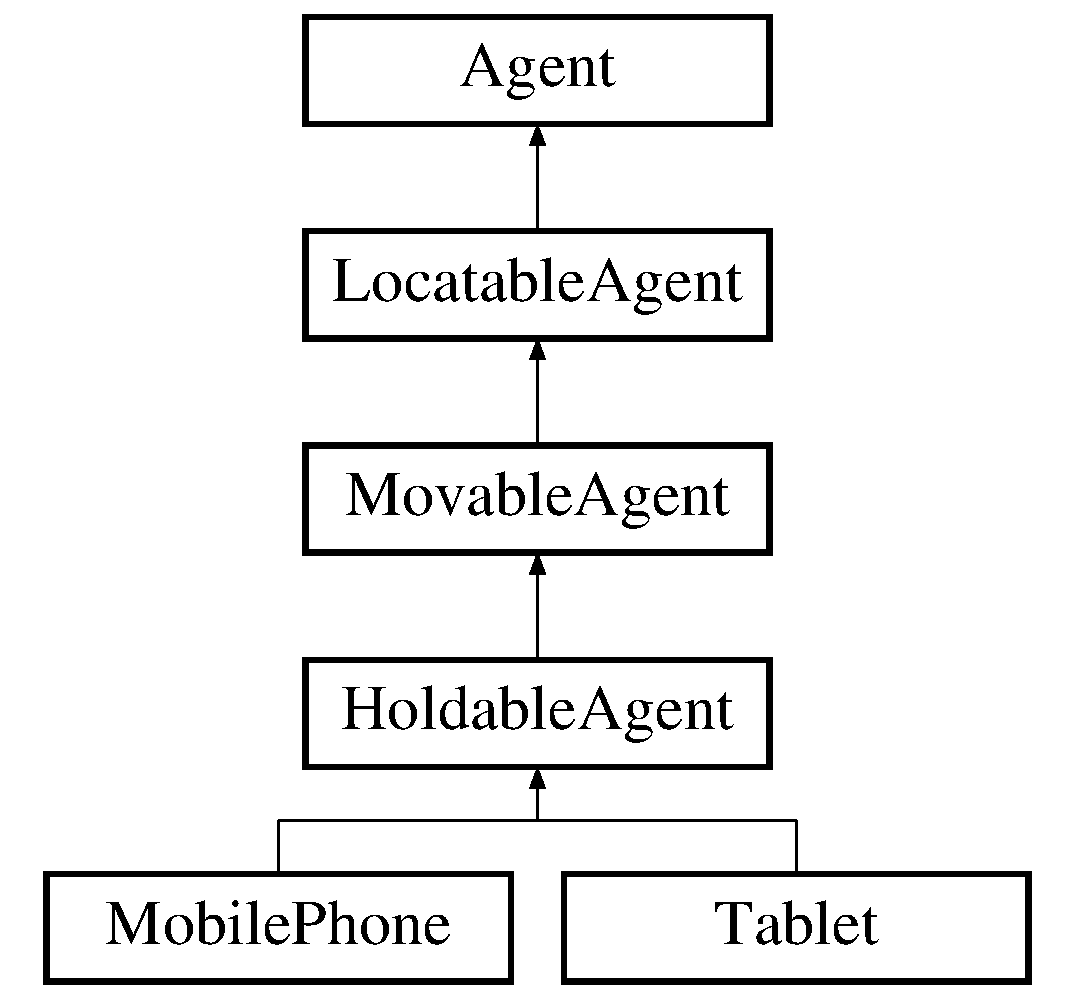
\includegraphics[height=5.000000cm]{class_holdable_agent}
\end{center}
\end{figure}
\subsection*{Public Types}
\begin{DoxyCompactItemize}
\item 
enum \textbf{ C\+O\+N\+N\+E\+C\+T\+I\+O\+N\+\_\+\+T\+Y\+PE} \{ \textbf{ U\+S\+I\+N\+G\+\_\+\+P\+O\+W\+ER}, 
\textbf{ U\+S\+I\+N\+G\+\_\+\+S\+I\+G\+N\+A\+L\+\_\+\+Q\+U\+A\+L\+I\+TY}, 
\textbf{ U\+N\+K\+N\+O\+WN}
 \}
\end{DoxyCompactItemize}
\subsection*{Public Member Functions}
\begin{DoxyCompactItemize}
\item 
\textbf{ Holdable\+Agent} (\textbf{ Map} $\ast$m, long id, Point $\ast$init\+Position, \textbf{ Agent} $\ast$holder, \textbf{ Clock} $\ast$clock)
\item 
\textbf{ Holdable\+Agent} (const \textbf{ Holdable\+Agent} \&h)
\item 
virtual \textbf{ $\sim$\+Holdable\+Agent} ()
\item 
\textbf{ Agent} $\ast$ \textbf{ get\+Holder} () const
\item 
void \textbf{ set\+Holder} (\textbf{ Agent} $\ast$holder)
\item 
string \textbf{ get\+Name} () override
\item 
string \textbf{ to\+String} () override
\item 
virtual bool \textbf{ try\+Connect} (\textbf{ C\+O\+N\+N\+E\+C\+T\+I\+O\+N\+\_\+\+T\+Y\+PE} type)=0
\item 
virtual bool \textbf{ is\+Connected} () const
\item 
void \textbf{ set\+Location} (Point $\ast$location) override
\item 
vector$<$ \textbf{ Antenna} $\ast$ $>$ \textbf{ get\+Antennas} () const
\end{DoxyCompactItemize}
\subsection*{Private Attributes}
\begin{DoxyCompactItemize}
\item 
\textbf{ Agent} $\ast$ \textbf{ m\+\_\+holder}
\item 
vector$<$ \textbf{ Antenna} $\ast$ $>$ \textbf{ m\+\_\+antennas}
\end{DoxyCompactItemize}


\subsection{Detailed Description}


Definition at line 21 of file Holdable\+Agent.\+h.



\subsection{Member Enumeration Documentation}
\mbox{\label{class_holdable_agent_ae2c334b004d7b9c5a999cf2618e4e518}} 
\index{HoldableAgent@{HoldableAgent}!CONNECTION\_TYPE@{CONNECTION\_TYPE}}
\index{CONNECTION\_TYPE@{CONNECTION\_TYPE}!HoldableAgent@{HoldableAgent}}
\subsubsection{CONNECTION\_TYPE}
{\footnotesize\ttfamily enum \textbf{ Holdable\+Agent\+::\+C\+O\+N\+N\+E\+C\+T\+I\+O\+N\+\_\+\+T\+Y\+PE}}

\begin{DoxyEnumFields}{Enumerator}
\raisebox{\heightof{T}}[0pt][0pt]{\index{USING\_POWER@{USING\_POWER}!HoldableAgent@{HoldableAgent}}\index{HoldableAgent@{HoldableAgent}!USING\_POWER@{USING\_POWER}}}\mbox{\label{class_holdable_agent_ae2c334b004d7b9c5a999cf2618e4e518ab8f4a3956d88a54e0aad08e89e203fd6}} 
U\+S\+I\+N\+G\+\_\+\+P\+O\+W\+ER&\\
\hline

\raisebox{\heightof{T}}[0pt][0pt]{\index{USING\_SIGNAL\_QUALITY@{USING\_SIGNAL\_QUALITY}!HoldableAgent@{HoldableAgent}}\index{HoldableAgent@{HoldableAgent}!USING\_SIGNAL\_QUALITY@{USING\_SIGNAL\_QUALITY}}}\mbox{\label{class_holdable_agent_ae2c334b004d7b9c5a999cf2618e4e518a93c5b260edf949c65b96fec443c33f2b}} 
U\+S\+I\+N\+G\+\_\+\+S\+I\+G\+N\+A\+L\+\_\+\+Q\+U\+A\+L\+I\+TY&\\
\hline

\raisebox{\heightof{T}}[0pt][0pt]{\index{UNKNOWN@{UNKNOWN}!HoldableAgent@{HoldableAgent}}\index{HoldableAgent@{HoldableAgent}!UNKNOWN@{UNKNOWN}}}\mbox{\label{class_holdable_agent_ae2c334b004d7b9c5a999cf2618e4e518a6bdb1529a2032a4648226328e179f552}} 
U\+N\+K\+N\+O\+WN&\\
\hline

\end{DoxyEnumFields}


Definition at line 25 of file Holdable\+Agent.\+h.



\subsection{Constructor \& Destructor Documentation}
\mbox{\label{class_holdable_agent_ab5060ddcd08291c60b49fec22d6bd6f3}} 
\index{HoldableAgent@{HoldableAgent}!HoldableAgent@{HoldableAgent}}
\index{HoldableAgent@{HoldableAgent}!HoldableAgent@{HoldableAgent}}
\subsubsection{HoldableAgent()\hspace{0.1cm}{\footnotesize\ttfamily [1/2]}}
{\footnotesize\ttfamily Holdable\+Agent\+::\+Holdable\+Agent (\begin{DoxyParamCaption}\item[{\textbf{ Map} $\ast$}]{m,  }\item[{long}]{id,  }\item[{Point $\ast$}]{init\+Position,  }\item[{\textbf{ Agent} $\ast$}]{holder,  }\item[{\textbf{ Clock} $\ast$}]{clock }\end{DoxyParamCaption})\hspace{0.3cm}{\ttfamily [explicit]}}



Definition at line 16 of file Holdable\+Agent.\+cpp.

\mbox{\label{class_holdable_agent_a9b7c1494266c0a807d809461b59ced80}} 
\index{HoldableAgent@{HoldableAgent}!HoldableAgent@{HoldableAgent}}
\index{HoldableAgent@{HoldableAgent}!HoldableAgent@{HoldableAgent}}
\subsubsection{HoldableAgent()\hspace{0.1cm}{\footnotesize\ttfamily [2/2]}}
{\footnotesize\ttfamily Holdable\+Agent\+::\+Holdable\+Agent (\begin{DoxyParamCaption}\item[{const \textbf{ Holdable\+Agent} \&}]{h }\end{DoxyParamCaption})}



Definition at line 22 of file Holdable\+Agent.\+cpp.



References get\+Antennas(), get\+Holder(), m\+\_\+antennas, and m\+\_\+holder.

\mbox{\label{class_holdable_agent_ab529d1f070a574375a79baadc89e9b78}} 
\index{HoldableAgent@{HoldableAgent}!````~HoldableAgent@{$\sim$HoldableAgent}}
\index{````~HoldableAgent@{$\sim$HoldableAgent}!HoldableAgent@{HoldableAgent}}
\subsubsection{$\sim$HoldableAgent()}
{\footnotesize\ttfamily Holdable\+Agent\+::$\sim$\+Holdable\+Agent (\begin{DoxyParamCaption}{ }\end{DoxyParamCaption})\hspace{0.3cm}{\ttfamily [virtual]}}



Definition at line 29 of file Holdable\+Agent.\+cpp.



\subsection{Member Function Documentation}
\mbox{\label{class_holdable_agent_af04b66d8148877c40e1fa0a5fef4b546}} 
\index{HoldableAgent@{HoldableAgent}!getAntennas@{getAntennas}}
\index{getAntennas@{getAntennas}!HoldableAgent@{HoldableAgent}}
\subsubsection{getAntennas()}
{\footnotesize\ttfamily vector$<$ \textbf{ Antenna} $\ast$ $>$ Holdable\+Agent\+::get\+Antennas (\begin{DoxyParamCaption}{ }\end{DoxyParamCaption}) const}



Definition at line 54 of file Holdable\+Agent.\+cpp.



References m\+\_\+antennas.



Referenced by Holdable\+Agent().

\mbox{\label{class_holdable_agent_a4fdf36fd8fb79a168360ebf74b9ba61d}} 
\index{HoldableAgent@{HoldableAgent}!getHolder@{getHolder}}
\index{getHolder@{getHolder}!HoldableAgent@{HoldableAgent}}
\subsubsection{getHolder()}
{\footnotesize\ttfamily \textbf{ Agent} $\ast$ Holdable\+Agent\+::get\+Holder (\begin{DoxyParamCaption}{ }\end{DoxyParamCaption}) const}



Definition at line 33 of file Holdable\+Agent.\+cpp.



References m\+\_\+holder.



Referenced by Holdable\+Agent().

\mbox{\label{class_holdable_agent_a089a15867a877d3a4cb510169c32d682}} 
\index{HoldableAgent@{HoldableAgent}!getName@{getName}}
\index{getName@{getName}!HoldableAgent@{HoldableAgent}}
\subsubsection{getName()}
{\footnotesize\ttfamily string Holdable\+Agent\+::get\+Name (\begin{DoxyParamCaption}{ }\end{DoxyParamCaption})\hspace{0.3cm}{\ttfamily [inline]}, {\ttfamily [override]}, {\ttfamily [virtual]}}



Implements \textbf{ Agent} \doxyref{}{p.}{class_agent_aa24682b2e0c8031d0637c156f6bee0e0}.



Reimplemented in \textbf{ Mobile\+Phone} \doxyref{}{p.}{class_mobile_phone_aa4f050bb755994fadfeab94c1f2147f7}, and \textbf{ Tablet} \doxyref{}{p.}{class_tablet_a2cac00cd9efca5b8adeff28ae5827970}.



Definition at line 34 of file Holdable\+Agent.\+h.

\mbox{\label{class_holdable_agent_a5d7b3db4bf6044736d80de1677afdeec}} 
\index{HoldableAgent@{HoldableAgent}!isConnected@{isConnected}}
\index{isConnected@{isConnected}!HoldableAgent@{HoldableAgent}}
\subsubsection{isConnected()}
{\footnotesize\ttfamily bool Holdable\+Agent\+::is\+Connected (\begin{DoxyParamCaption}{ }\end{DoxyParamCaption}) const\hspace{0.3cm}{\ttfamily [virtual]}}



Definition at line 50 of file Holdable\+Agent.\+cpp.



References m\+\_\+antennas.

\mbox{\label{class_holdable_agent_a39b53c9c6cacca716f38fccc520e9f52}} 
\index{HoldableAgent@{HoldableAgent}!setHolder@{setHolder}}
\index{setHolder@{setHolder}!HoldableAgent@{HoldableAgent}}
\subsubsection{setHolder()}
{\footnotesize\ttfamily void Holdable\+Agent\+::set\+Holder (\begin{DoxyParamCaption}\item[{\textbf{ Agent} $\ast$}]{holder }\end{DoxyParamCaption})}



Definition at line 37 of file Holdable\+Agent.\+cpp.



References Locatable\+Agent\+::get\+Location(), m\+\_\+holder, set\+Location(), and Movable\+Agent\+::set\+Speed().

\mbox{\label{class_holdable_agent_aec98d2fe325b48d9a84ad3dad44700e0}} 
\index{HoldableAgent@{HoldableAgent}!setLocation@{setLocation}}
\index{setLocation@{setLocation}!HoldableAgent@{HoldableAgent}}
\subsubsection{setLocation()}
{\footnotesize\ttfamily void Holdable\+Agent\+::set\+Location (\begin{DoxyParamCaption}\item[{Point $\ast$}]{location }\end{DoxyParamCaption})\hspace{0.3cm}{\ttfamily [override]}, {\ttfamily [virtual]}}



Reimplemented from \textbf{ Locatable\+Agent} \doxyref{}{p.}{class_locatable_agent_a4185a45957d529a7f57d19ea294cae81}.



Definition at line 58 of file Holdable\+Agent.\+cpp.



References Locatable\+Agent\+::set\+Location(), and try\+Connect().



Referenced by set\+Holder(), and Person\+::set\+Location().

\mbox{\label{class_holdable_agent_a3fee3021111198ac01469a715093ab88}} 
\index{HoldableAgent@{HoldableAgent}!toString@{toString}}
\index{toString@{toString}!HoldableAgent@{HoldableAgent}}
\subsubsection{toString()}
{\footnotesize\ttfamily string Holdable\+Agent\+::to\+String (\begin{DoxyParamCaption}{ }\end{DoxyParamCaption})\hspace{0.3cm}{\ttfamily [override]}, {\ttfamily [virtual]}}



Implements \textbf{ Agent} \doxyref{}{p.}{class_agent_a530b76f9163b2b8c19e7cdf8065888ac}.



Reimplemented in \textbf{ Mobile\+Phone} \doxyref{}{p.}{class_mobile_phone_a3e4bf0a37331042084ae703666f8fb7c}, and \textbf{ Tablet} \doxyref{}{p.}{class_tablet_a90880cd8f4a4afd451645e6e1dc86c5b}.



Definition at line 63 of file Holdable\+Agent.\+cpp.



References Agent\+::get\+Id(), m\+\_\+holder, and Movable\+Agent\+::to\+String().



Referenced by Tablet\+::to\+String(), and Mobile\+Phone\+::to\+String().

\mbox{\label{class_holdable_agent_a3f6500c10b054ca06a7800d4b01c5308}} 
\index{HoldableAgent@{HoldableAgent}!tryConnect@{tryConnect}}
\index{tryConnect@{tryConnect}!HoldableAgent@{HoldableAgent}}
\subsubsection{tryConnect()}
{\footnotesize\ttfamily virtual bool Holdable\+Agent\+::try\+Connect (\begin{DoxyParamCaption}\item[{\textbf{ C\+O\+N\+N\+E\+C\+T\+I\+O\+N\+\_\+\+T\+Y\+PE}}]{type }\end{DoxyParamCaption})\hspace{0.3cm}{\ttfamily [pure virtual]}}



Implemented in \textbf{ Mobile\+Phone} \doxyref{}{p.}{class_mobile_phone_a384f2a32e076dd34fdd1e814e1a48c11}, and \textbf{ Tablet} \doxyref{}{p.}{class_tablet_a4a08098f3acddd3167fc9633deabb809}.



Referenced by set\+Location().



\subsection{Member Data Documentation}
\mbox{\label{class_holdable_agent_a5f104212204e4c6761bed1d61fab100b}} 
\index{HoldableAgent@{HoldableAgent}!m\_antennas@{m\_antennas}}
\index{m\_antennas@{m\_antennas}!HoldableAgent@{HoldableAgent}}
\subsubsection{m\_antennas}
{\footnotesize\ttfamily vector$<$\textbf{ Antenna}$\ast$$>$ Holdable\+Agent\+::m\+\_\+antennas\hspace{0.3cm}{\ttfamily [private]}}



Definition at line 47 of file Holdable\+Agent.\+h.



Referenced by get\+Antennas(), Holdable\+Agent(), and is\+Connected().

\mbox{\label{class_holdable_agent_ae9c449c1831f933b5b6b6f71e425279b}} 
\index{HoldableAgent@{HoldableAgent}!m\_holder@{m\_holder}}
\index{m\_holder@{m\_holder}!HoldableAgent@{HoldableAgent}}
\subsubsection{m\_holder}
{\footnotesize\ttfamily \textbf{ Agent}$\ast$ Holdable\+Agent\+::m\+\_\+holder\hspace{0.3cm}{\ttfamily [private]}}



Definition at line 46 of file Holdable\+Agent.\+h.



Referenced by get\+Holder(), Holdable\+Agent(), set\+Holder(), and to\+String().



The documentation for this class was generated from the following files\+:\begin{DoxyCompactItemize}
\item 
include/\textbf{ Holdable\+Agent.\+h}\item 
src/\textbf{ Holdable\+Agent.\+cpp}\end{DoxyCompactItemize}

\hypertarget{class_i_d_generator}{}\section{I\+D\+Generator Class Reference}
\label{class_i_d_generator}\index{I\+D\+Generator@{I\+D\+Generator}}


{\ttfamily \#include $<$I\+D\+Generator.\+h$>$}



Collaboration diagram for I\+D\+Generator\+:\nopagebreak
\begin{figure}[H]
\begin{center}
\leavevmode
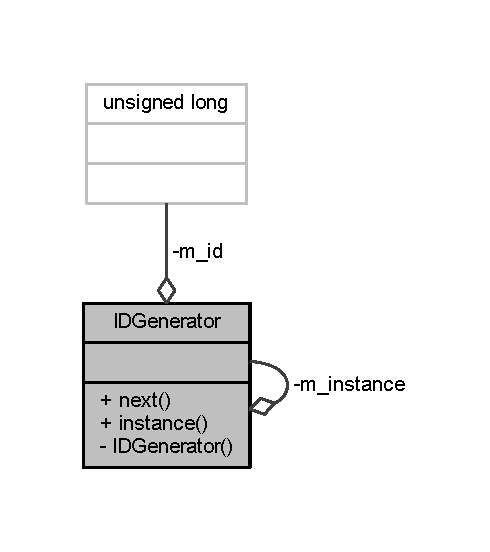
\includegraphics[width=235pt]{class_i_d_generator__coll__graph}
\end{center}
\end{figure}
\subsection*{Public Member Functions}
\begin{DoxyCompactItemize}
\item 
unsigned long \hyperlink{class_i_d_generator_a99d8cabb2ec6a17888a8ccbe9c85fee0}{next} ()
\end{DoxyCompactItemize}
\subsection*{Static Public Member Functions}
\begin{DoxyCompactItemize}
\item 
static \hyperlink{class_i_d_generator}{I\+D\+Generator} $\ast$ \hyperlink{class_i_d_generator_ad852c6dadc89e1020e4b3932f5a97bb3}{instance} ()
\end{DoxyCompactItemize}
\subsection*{Private Member Functions}
\begin{DoxyCompactItemize}
\item 
\hyperlink{class_i_d_generator_a8209b55f50b469c47f977660a769b1da}{I\+D\+Generator} ()
\end{DoxyCompactItemize}
\subsection*{Private Attributes}
\begin{DoxyCompactItemize}
\item 
unsigned long \hyperlink{class_i_d_generator_ad0400380525f694b23ff675f4f170893}{m\+\_\+id}
\end{DoxyCompactItemize}
\subsection*{Static Private Attributes}
\begin{DoxyCompactItemize}
\item 
static \hyperlink{class_i_d_generator}{I\+D\+Generator} $\ast$ \hyperlink{class_i_d_generator_a316bacdda67f4cf9bf73fcbd9bf94245}{m\+\_\+instance}
\end{DoxyCompactItemize}


\subsection{Detailed Description}
This singleton class is used to generate unique identifiers for all agents in the simulation. The ids are unsigned long integers. 

\subsection{Constructor \& Destructor Documentation}
\mbox{\Hypertarget{class_i_d_generator_a8209b55f50b469c47f977660a769b1da}\label{class_i_d_generator_a8209b55f50b469c47f977660a769b1da}} 
\index{I\+D\+Generator@{I\+D\+Generator}!I\+D\+Generator@{I\+D\+Generator}}
\index{I\+D\+Generator@{I\+D\+Generator}!I\+D\+Generator@{I\+D\+Generator}}
\subsubsection{\texorpdfstring{I\+D\+Generator()}{IDGenerator()}}
{\footnotesize\ttfamily I\+D\+Generator\+::\+I\+D\+Generator (\begin{DoxyParamCaption}{ }\end{DoxyParamCaption})\hspace{0.3cm}{\ttfamily [inline]}, {\ttfamily [private]}}

Here is the caller graph for this function\+:\nopagebreak
\begin{figure}[H]
\begin{center}
\leavevmode
\includegraphics[width=350pt]{class_i_d_generator_a8209b55f50b469c47f977660a769b1da_icgraph}
\end{center}
\end{figure}


\subsection{Member Function Documentation}
\mbox{\Hypertarget{class_i_d_generator_ad852c6dadc89e1020e4b3932f5a97bb3}\label{class_i_d_generator_ad852c6dadc89e1020e4b3932f5a97bb3}} 
\index{I\+D\+Generator@{I\+D\+Generator}!instance@{instance}}
\index{instance@{instance}!I\+D\+Generator@{I\+D\+Generator}}
\subsubsection{\texorpdfstring{instance()}{instance()}}
{\footnotesize\ttfamily static \hyperlink{class_i_d_generator}{I\+D\+Generator}$\ast$ I\+D\+Generator\+::instance (\begin{DoxyParamCaption}{ }\end{DoxyParamCaption})\hspace{0.3cm}{\ttfamily [inline]}, {\ttfamily [static]}}

Returns an instance of this class. \begin{DoxyReturn}{Returns}
an instance of this class. 
\end{DoxyReturn}
Here is the call graph for this function\+:\nopagebreak
\begin{figure}[H]
\begin{center}
\leavevmode
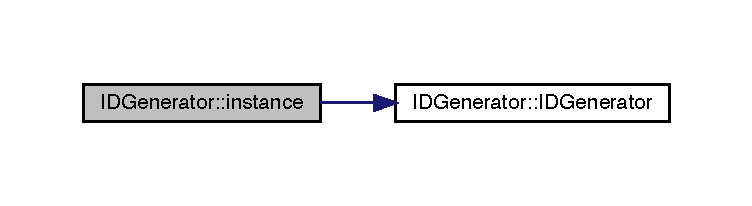
\includegraphics[width=350pt]{class_i_d_generator_ad852c6dadc89e1020e4b3932f5a97bb3_cgraph}
\end{center}
\end{figure}
\mbox{\Hypertarget{class_i_d_generator_a99d8cabb2ec6a17888a8ccbe9c85fee0}\label{class_i_d_generator_a99d8cabb2ec6a17888a8ccbe9c85fee0}} 
\index{I\+D\+Generator@{I\+D\+Generator}!next@{next}}
\index{next@{next}!I\+D\+Generator@{I\+D\+Generator}}
\subsubsection{\texorpdfstring{next()}{next()}}
{\footnotesize\ttfamily unsigned long I\+D\+Generator\+::next (\begin{DoxyParamCaption}{ }\end{DoxyParamCaption})\hspace{0.3cm}{\ttfamily [inline]}}

Generates the next unique identifier. \begin{DoxyReturn}{Returns}
a unique identifier. 
\end{DoxyReturn}


\subsection{Member Data Documentation}
\mbox{\Hypertarget{class_i_d_generator_ad0400380525f694b23ff675f4f170893}\label{class_i_d_generator_ad0400380525f694b23ff675f4f170893}} 
\index{I\+D\+Generator@{I\+D\+Generator}!m\+\_\+id@{m\+\_\+id}}
\index{m\+\_\+id@{m\+\_\+id}!I\+D\+Generator@{I\+D\+Generator}}
\subsubsection{\texorpdfstring{m\+\_\+id}{m\_id}}
{\footnotesize\ttfamily unsigned long I\+D\+Generator\+::m\+\_\+id\hspace{0.3cm}{\ttfamily [private]}}

\mbox{\Hypertarget{class_i_d_generator_a316bacdda67f4cf9bf73fcbd9bf94245}\label{class_i_d_generator_a316bacdda67f4cf9bf73fcbd9bf94245}} 
\index{I\+D\+Generator@{I\+D\+Generator}!m\+\_\+instance@{m\+\_\+instance}}
\index{m\+\_\+instance@{m\+\_\+instance}!I\+D\+Generator@{I\+D\+Generator}}
\subsubsection{\texorpdfstring{m\+\_\+instance}{m\_instance}}
{\footnotesize\ttfamily \hyperlink{class_i_d_generator}{I\+D\+Generator}$\ast$ I\+D\+Generator\+::m\+\_\+instance\hspace{0.3cm}{\ttfamily [static]}, {\ttfamily [private]}}



The documentation for this class was generated from the following file\+:\begin{DoxyCompactItemize}
\item 
include/\hyperlink{_i_d_generator_8h}{I\+D\+Generator.\+h}\end{DoxyCompactItemize}

\section{Immovable\+Agent Class Reference}
\label{class_immovable_agent}\index{Immovable\+Agent@{Immovable\+Agent}}


{\ttfamily \#include $<$Immovable\+Agent.\+h$>$}



Inheritance diagram for Immovable\+Agent\+:
% FIG 0


Collaboration diagram for Immovable\+Agent\+:
% FIG 1
\subsection*{Public Member Functions}
\begin{DoxyCompactItemize}
\item 
\textbf{ Immovable\+Agent} (\textbf{ Map} $\ast$m, long id, Point $\ast$initial\+Position, \textbf{ Clock} $\ast$clock)
\item 
virtual \textbf{ $\sim$\+Immovable\+Agent} ()
\item 
string \textbf{ to\+String} () override
\item 
string \textbf{ get\+Name} () override
\end{DoxyCompactItemize}


\subsection{Detailed Description}


Definition at line 23 of file Immovable\+Agent.\+h.



\subsection{Constructor \& Destructor Documentation}
\mbox{\label{class_immovable_agent_aca3d3a6d6608a1e639a57e84c94e336e}} 
\index{Immovable\+Agent@{Immovable\+Agent}!Immovable\+Agent@{Immovable\+Agent}}
\index{Immovable\+Agent@{Immovable\+Agent}!Immovable\+Agent@{Immovable\+Agent}}
\subsubsection{Immovable\+Agent()}
{\footnotesize\ttfamily Immovable\+Agent\+::\+Immovable\+Agent (\begin{DoxyParamCaption}\item[{\textbf{ Map} $\ast$}]{m,  }\item[{long}]{id,  }\item[{Point $\ast$}]{initial\+Position,  }\item[{\textbf{ Clock} $\ast$}]{clock }\end{DoxyParamCaption})\hspace{0.3cm}{\ttfamily [explicit]}}



Definition at line 17 of file Immovable\+Agent.\+cpp.

\mbox{\label{class_immovable_agent_af8bf8c3a8a322decc4ced38cb1296fee}} 
\index{Immovable\+Agent@{Immovable\+Agent}!````~Immovable\+Agent@{$\sim$\+Immovable\+Agent}}
\index{````~Immovable\+Agent@{$\sim$\+Immovable\+Agent}!Immovable\+Agent@{Immovable\+Agent}}
\subsubsection{$\sim$\+Immovable\+Agent()}
{\footnotesize\ttfamily Immovable\+Agent\+::$\sim$\+Immovable\+Agent (\begin{DoxyParamCaption}{ }\end{DoxyParamCaption})\hspace{0.3cm}{\ttfamily [virtual]}}



Definition at line 22 of file Immovable\+Agent.\+cpp.



\subsection{Member Function Documentation}
\mbox{\label{class_immovable_agent_a35b43ab9d6cd845a0ada5b95784994f0}} 
\index{Immovable\+Agent@{Immovable\+Agent}!get\+Name@{get\+Name}}
\index{get\+Name@{get\+Name}!Immovable\+Agent@{Immovable\+Agent}}
\subsubsection{get\+Name()}
{\footnotesize\ttfamily string Immovable\+Agent\+::get\+Name (\begin{DoxyParamCaption}{ }\end{DoxyParamCaption})\hspace{0.3cm}{\ttfamily [inline]}, {\ttfamily [override]}, {\ttfamily [virtual]}}

This function is used to get the name of the class. It is a pure virtual function, all subclasses implment it and return the actual name of the class. \begin{DoxyReturn}{Returns}
the name of the class. 
\end{DoxyReturn}


Implements \textbf{ Agent} \doxyref{}{p.}{class_agent_aa24682b2e0c8031d0637c156f6bee0e0}.



Definition at line 30 of file Immovable\+Agent.\+h.

\mbox{\label{class_immovable_agent_a94ec08f8c08ec2b4cecf5ef27b00fa32}} 
\index{Immovable\+Agent@{Immovable\+Agent}!to\+String@{to\+String}}
\index{to\+String@{to\+String}!Immovable\+Agent@{Immovable\+Agent}}
\subsubsection{to\+String()}
{\footnotesize\ttfamily string Immovable\+Agent\+::to\+String (\begin{DoxyParamCaption}{ }\end{DoxyParamCaption})\hspace{0.3cm}{\ttfamily [override]}, {\ttfamily [virtual]}}

Builds a string with of the relevant information of the class. It is useful to output on the console or in a file the description of concrete agents. \begin{DoxyReturn}{Returns}
a string representation of the class content. The values of the members are written in this string. 
\end{DoxyReturn}


Implements \textbf{ Agent} \doxyref{}{p.}{class_agent_a530b76f9163b2b8c19e7cdf8065888ac}.



Definition at line 26 of file Immovable\+Agent.\+cpp.



References Locatable\+Agent\+::to\+String().



Referenced by Antenna\+::to\+String().

Here is the call graph for this function\+:
% FIG 2


The documentation for this class was generated from the following files\+:\begin{DoxyCompactItemize}
\item 
include/\textbf{ Immovable\+Agent.\+h}\item 
src/\textbf{ Immovable\+Agent.\+cpp}\end{DoxyCompactItemize}

\section{Input\+Parser Class Reference}
\label{class_input_parser}\index{InputParser@{InputParser}}


{\ttfamily \#include $<$Input\+Parser.\+h$>$}

\subsection*{Public Member Functions}
\begin{DoxyCompactItemize}
\item 
\textbf{ Input\+Parser} (int \&argc, char $\ast$$\ast$argv)
\item 
const string \& \textbf{ get\+Cmd\+Option} (const string \&option) const
\item 
bool \textbf{ cmd\+Option\+Exists} (const string \&option) const
\end{DoxyCompactItemize}
\subsection*{Private Attributes}
\begin{DoxyCompactItemize}
\item 
vector$<$ string $>$ \textbf{ tokens}
\end{DoxyCompactItemize}


\subsection{Detailed Description}


Definition at line 20 of file Input\+Parser.\+h.



\subsection{Constructor \& Destructor Documentation}
\mbox{\label{class_input_parser_af9fa5ead1f28b5294a713410df5b9531}} 
\index{InputParser@{InputParser}!InputParser@{InputParser}}
\index{InputParser@{InputParser}!InputParser@{InputParser}}
\subsubsection{InputParser()}
{\footnotesize\ttfamily Input\+Parser\+::\+Input\+Parser (\begin{DoxyParamCaption}\item[{int \&}]{argc,  }\item[{char $\ast$$\ast$}]{argv }\end{DoxyParamCaption})}



Definition at line 14 of file Input\+Parser.\+cpp.



References tokens.



\subsection{Member Function Documentation}
\mbox{\label{class_input_parser_ad3d06a9c59e91f425295bdc8408e0544}} 
\index{InputParser@{InputParser}!cmdOptionExists@{cmdOptionExists}}
\index{cmdOptionExists@{cmdOptionExists}!InputParser@{InputParser}}
\subsubsection{cmdOptionExists()}
{\footnotesize\ttfamily bool Input\+Parser\+::cmd\+Option\+Exists (\begin{DoxyParamCaption}\item[{const string \&}]{option }\end{DoxyParamCaption}) const}



Definition at line 29 of file Input\+Parser.\+cpp.



References tokens.

\mbox{\label{class_input_parser_a494c1de8c06fbb5a88343686e36fbf50}} 
\index{InputParser@{InputParser}!getCmdOption@{getCmdOption}}
\index{getCmdOption@{getCmdOption}!InputParser@{InputParser}}
\subsubsection{getCmdOption()}
{\footnotesize\ttfamily const string \& Input\+Parser\+::get\+Cmd\+Option (\begin{DoxyParamCaption}\item[{const string \&}]{option }\end{DoxyParamCaption}) const}



Definition at line 19 of file Input\+Parser.\+cpp.



References tokens.



\subsection{Member Data Documentation}
\mbox{\label{class_input_parser_a4bd1105d6fc64bd0e825dc2e34515d75}} 
\index{InputParser@{InputParser}!tokens@{tokens}}
\index{tokens@{tokens}!InputParser@{InputParser}}
\subsubsection{tokens}
{\footnotesize\ttfamily vector$<$string$>$ Input\+Parser\+::tokens\hspace{0.3cm}{\ttfamily [private]}}



Definition at line 26 of file Input\+Parser.\+h.



Referenced by cmd\+Option\+Exists(), get\+Cmd\+Option(), and Input\+Parser().



The documentation for this class was generated from the following files\+:\begin{DoxyCompactItemize}
\item 
include/\textbf{ Input\+Parser.\+h}\item 
src/\textbf{ Input\+Parser.\+cpp}\end{DoxyCompactItemize}

\section{tinyxml2\+:\+:Mem\+PoolT$<$ I\+T\+E\+M\+\_\+\+S\+I\+ZE $>$\+:\+:Item Union Reference}
\label{uniontinyxml2_1_1_mem_pool_t_1_1_item}\index{tinyxml2\+::\+Mem\+Pool\+T$<$ I\+T\+E\+M\+\_\+\+S\+I\+Z\+E $>$\+::\+Item@{tinyxml2\+::\+Mem\+Pool\+T$<$ I\+T\+E\+M\+\_\+\+S\+I\+Z\+E $>$\+::\+Item}}


Collaboration diagram for tinyxml2\+:\+:Mem\+PoolT$<$ I\+T\+E\+M\+\_\+\+S\+I\+ZE $>$\+:\+:Item\+:
% FIG 0
\subsection*{Public Attributes}
\begin{DoxyCompactItemize}
\item 
\textbf{ Item} $\ast$ \textbf{ next}
\item 
char \textbf{ item\+Data} [I\+T\+E\+M\+\_\+\+S\+I\+ZE]
\end{DoxyCompactItemize}


\subsection{Detailed Description}
\subsubsection*{template$<$int I\+T\+E\+M\+\_\+\+S\+I\+ZE$>$\newline
union tinyxml2\+::\+Mem\+Pool\+T$<$ I\+T\+E\+M\+\_\+\+S\+I\+Z\+E $>$\+::\+Item}



Definition at line 443 of file tinyxml2.\+h.



\subsection{Member Data Documentation}
\mbox{\label{uniontinyxml2_1_1_mem_pool_t_1_1_item_aff63ccc8d7b05035820b83e1f0fa8037}} 
\index{tinyxml2\+::\+Mem\+Pool\+T\+::\+Item@{tinyxml2\+::\+Mem\+Pool\+T\+::\+Item}!item\+Data@{item\+Data}}
\index{item\+Data@{item\+Data}!tinyxml2\+::\+Mem\+Pool\+T\+::\+Item@{tinyxml2\+::\+Mem\+Pool\+T\+::\+Item}}
\subsubsection{item\+Data}
{\footnotesize\ttfamily template$<$int I\+T\+E\+M\+\_\+\+S\+I\+ZE$>$ \\
char \textbf{ tinyxml2\+::\+Mem\+PoolT}$<$ I\+T\+E\+M\+\_\+\+S\+I\+ZE $>$\+::Item\+::item\+Data[I\+T\+E\+M\+\_\+\+S\+I\+ZE]}



Definition at line 445 of file tinyxml2.\+h.

\mbox{\label{uniontinyxml2_1_1_mem_pool_t_1_1_item_a5620107f518c60d6619e8662d4c9d643}} 
\index{tinyxml2\+::\+Mem\+Pool\+T\+::\+Item@{tinyxml2\+::\+Mem\+Pool\+T\+::\+Item}!next@{next}}
\index{next@{next}!tinyxml2\+::\+Mem\+Pool\+T\+::\+Item@{tinyxml2\+::\+Mem\+Pool\+T\+::\+Item}}
\subsubsection{next}
{\footnotesize\ttfamily template$<$int I\+T\+E\+M\+\_\+\+S\+I\+ZE$>$ \\
\textbf{ Item}$\ast$ \textbf{ tinyxml2\+::\+Mem\+PoolT}$<$ I\+T\+E\+M\+\_\+\+S\+I\+ZE $>$\+::Item\+::next}



Definition at line 444 of file tinyxml2.\+h.



The documentation for this union was generated from the following file\+:\begin{DoxyCompactItemize}
\item 
include/\textbf{ tinyxml2.\+h}\end{DoxyCompactItemize}

\section{Locatable\+Agent Class Reference}
\label{class_locatable_agent}\index{LocatableAgent@{LocatableAgent}}


{\ttfamily \#include $<$Locatable\+Agent.\+h$>$}

Inheritance diagram for Locatable\+Agent\+:\begin{figure}[H]
\begin{center}
\leavevmode
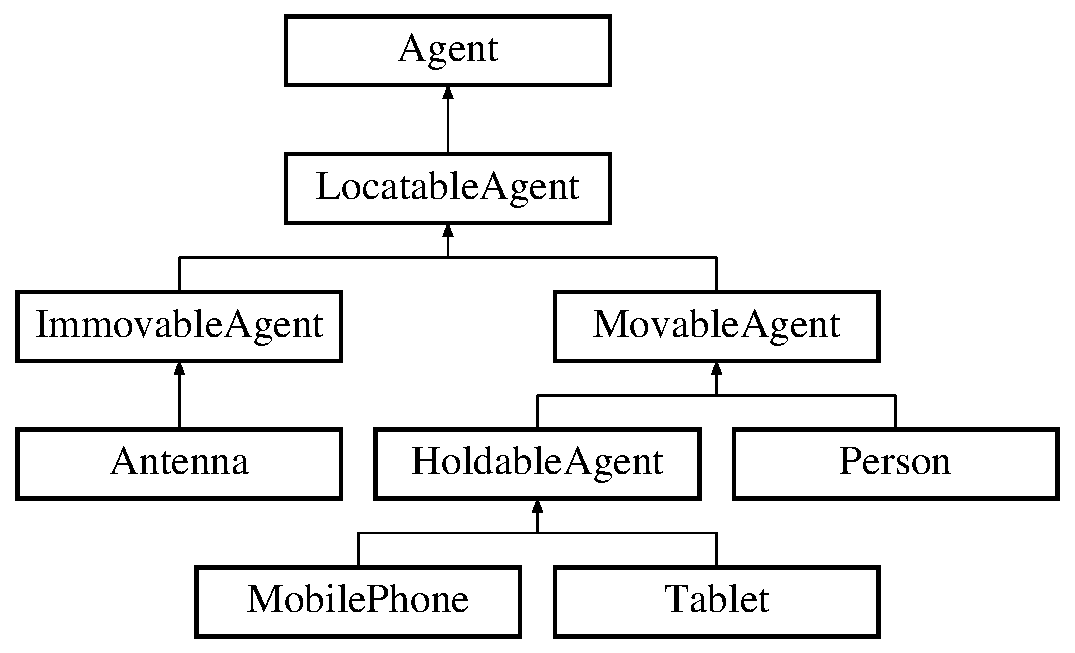
\includegraphics[height=5.000000cm]{class_locatable_agent}
\end{center}
\end{figure}
\subsection*{Public Member Functions}
\begin{DoxyCompactItemize}
\item 
\textbf{ Locatable\+Agent} (\textbf{ Map} $\ast$m, long id, Point $\ast$init\+Location, \textbf{ Clock} $\ast$clock)
\item 
virtual \textbf{ $\sim$\+Locatable\+Agent} ()
\item 
string \textbf{ get\+Name} () override
\item 
string \textbf{ to\+String} () override
\item 
virtual Point $\ast$ \textbf{ get\+Location} () const
\item 
virtual void \textbf{ set\+Location} (Point $\ast$location)
\item 
string \textbf{ dump\+Location} ()
\end{DoxyCompactItemize}
\subsection*{Private Attributes}
\begin{DoxyCompactItemize}
\item 
Point $\ast$ \textbf{ m\+\_\+location}
\end{DoxyCompactItemize}


\subsection{Detailed Description}


Definition at line 21 of file Locatable\+Agent.\+h.



\subsection{Constructor \& Destructor Documentation}
\mbox{\label{class_locatable_agent_ac499b75f07ffa4daf3da16488953533e}} 
\index{LocatableAgent@{LocatableAgent}!LocatableAgent@{LocatableAgent}}
\index{LocatableAgent@{LocatableAgent}!LocatableAgent@{LocatableAgent}}
\subsubsection{LocatableAgent()}
{\footnotesize\ttfamily Locatable\+Agent\+::\+Locatable\+Agent (\begin{DoxyParamCaption}\item[{\textbf{ Map} $\ast$}]{m,  }\item[{long}]{id,  }\item[{Point $\ast$}]{init\+Location,  }\item[{\textbf{ Clock} $\ast$}]{clock }\end{DoxyParamCaption})\hspace{0.3cm}{\ttfamily [explicit]}}



Definition at line 20 of file Locatable\+Agent.\+cpp.



References m\+\_\+location.

\mbox{\label{class_locatable_agent_a6a088f1e2c16a0b52e4a630868d4eae6}} 
\index{LocatableAgent@{LocatableAgent}!````~LocatableAgent@{$\sim$LocatableAgent}}
\index{````~LocatableAgent@{$\sim$LocatableAgent}!LocatableAgent@{LocatableAgent}}
\subsubsection{$\sim$LocatableAgent()}
{\footnotesize\ttfamily Locatable\+Agent\+::$\sim$\+Locatable\+Agent (\begin{DoxyParamCaption}{ }\end{DoxyParamCaption})\hspace{0.3cm}{\ttfamily [virtual]}}



Definition at line 26 of file Locatable\+Agent.\+cpp.



\subsection{Member Function Documentation}
\mbox{\label{class_locatable_agent_ab4436577328ce536ccba55d3068b2cf4}} 
\index{LocatableAgent@{LocatableAgent}!dumpLocation@{dumpLocation}}
\index{dumpLocation@{dumpLocation}!LocatableAgent@{LocatableAgent}}
\subsubsection{dumpLocation()}
{\footnotesize\ttfamily string Locatable\+Agent\+::dump\+Location (\begin{DoxyParamCaption}{ }\end{DoxyParamCaption})}



Definition at line 49 of file Locatable\+Agent.\+cpp.



References Agent\+::get\+Clock(), Clock\+::get\+Current\+Time(), Agent\+::get\+Id(), and get\+Location().



Referenced by World\+::run\+Simulation().

\mbox{\label{class_locatable_agent_a2392d365653e71cc35029fdebbfe18d9}} 
\index{LocatableAgent@{LocatableAgent}!getLocation@{getLocation}}
\index{getLocation@{getLocation}!LocatableAgent@{LocatableAgent}}
\subsubsection{getLocation()}
{\footnotesize\ttfamily Point $\ast$ Locatable\+Agent\+::get\+Location (\begin{DoxyParamCaption}{ }\end{DoxyParamCaption}) const\hspace{0.3cm}{\ttfamily [virtual]}}



Definition at line 31 of file Locatable\+Agent.\+cpp.



References m\+\_\+location.



Referenced by Antenna\+::compute\+Power(), Antenna\+::compute\+Signal\+Quality(), dump\+Location(), Tablet\+::move(), Person\+::move(), Person\+::random\+Walk(), Antenna\+::register\+Event(), Holdable\+Agent\+::set\+Holder(), to\+String(), and Mobile\+Phone\+::try\+Connect\+Naive\+Algorithm().

\mbox{\label{class_locatable_agent_ae2b9a1bd2e207a9aac95f4d13a17a9f9}} 
\index{LocatableAgent@{LocatableAgent}!getName@{getName}}
\index{getName@{getName}!LocatableAgent@{LocatableAgent}}
\subsubsection{getName()}
{\footnotesize\ttfamily string Locatable\+Agent\+::get\+Name (\begin{DoxyParamCaption}{ }\end{DoxyParamCaption})\hspace{0.3cm}{\ttfamily [inline]}, {\ttfamily [override]}, {\ttfamily [virtual]}}

This function is used to get the name of the class. It is a pure virtual function, all subclasses implment it and return the actual name of the class. \begin{DoxyReturn}{Returns}
the name of the class. 
\end{DoxyReturn}


Implements \textbf{ Agent} \doxyref{}{p.}{class_agent_aa24682b2e0c8031d0637c156f6bee0e0}.



Reimplemented in \textbf{ Person} \doxyref{}{p.}{class_person_a41c6a0cd763dc154841346e69f2d4b3e}, \textbf{ Movable\+Agent} \doxyref{}{p.}{class_movable_agent_af36b0e49e477cfcc60d801c11166a4f0}, \textbf{ Mobile\+Phone} \doxyref{}{p.}{class_mobile_phone_aa4f050bb755994fadfeab94c1f2147f7}, and \textbf{ Tablet} \doxyref{}{p.}{class_tablet_a2cac00cd9efca5b8adeff28ae5827970}.



Definition at line 27 of file Locatable\+Agent.\+h.

\mbox{\label{class_locatable_agent_a4185a45957d529a7f57d19ea294cae81}} 
\index{LocatableAgent@{LocatableAgent}!setLocation@{setLocation}}
\index{setLocation@{setLocation}!LocatableAgent@{LocatableAgent}}
\subsubsection{setLocation()}
{\footnotesize\ttfamily void Locatable\+Agent\+::set\+Location (\begin{DoxyParamCaption}\item[{Point $\ast$}]{location }\end{DoxyParamCaption})\hspace{0.3cm}{\ttfamily [virtual]}}



Reimplemented in \textbf{ Person} \doxyref{}{p.}{class_person_a2b31d3b9e0d9ed3b583d6d8d4c632518}, and \textbf{ Holdable\+Agent} \doxyref{}{p.}{class_holdable_agent_aec98d2fe325b48d9a84ad3dad44700e0}.



Definition at line 35 of file Locatable\+Agent.\+cpp.



References m\+\_\+location.



Referenced by Antenna\+::\+Antenna(), Holdable\+Agent\+::set\+Location(), and Person\+::set\+Location().

\mbox{\label{class_locatable_agent_a593b8f4eb5d0a812b725726c35335193}} 
\index{LocatableAgent@{LocatableAgent}!toString@{toString}}
\index{toString@{toString}!LocatableAgent@{LocatableAgent}}
\subsubsection{toString()}
{\footnotesize\ttfamily string Locatable\+Agent\+::to\+String (\begin{DoxyParamCaption}{ }\end{DoxyParamCaption})\hspace{0.3cm}{\ttfamily [override]}, {\ttfamily [virtual]}}

Builds a string with of the relevant information of the class. It is useful to output on the console or in a file the description of concrete agents. \begin{DoxyReturn}{Returns}
a string representation of the class content. The values of the members are written in this string. 
\end{DoxyReturn}


Implements \textbf{ Agent} \doxyref{}{p.}{class_agent_a530b76f9163b2b8c19e7cdf8065888ac}.



Reimplemented in \textbf{ Person} \doxyref{}{p.}{class_person_ac39b105901a2d4ce38ff5b548b1c349e}, \textbf{ Movable\+Agent} \doxyref{}{p.}{class_movable_agent_aa8a8424a9513e0d57f7d4b94e7a49552}, \textbf{ Mobile\+Phone} \doxyref{}{p.}{class_mobile_phone_a3e4bf0a37331042084ae703666f8fb7c}, and \textbf{ Tablet} \doxyref{}{p.}{class_tablet_a90880cd8f4a4afd451645e6e1dc86c5b}.



Definition at line 39 of file Locatable\+Agent.\+cpp.



References Agent\+::get\+Id(), get\+Location(), and m\+\_\+location.



Referenced by Immovable\+Agent\+::to\+String(), and Movable\+Agent\+::to\+String().



\subsection{Member Data Documentation}
\mbox{\label{class_locatable_agent_a2a76ba315733ab26f19229a71071704d}} 
\index{LocatableAgent@{LocatableAgent}!m\_location@{m\_location}}
\index{m\_location@{m\_location}!LocatableAgent@{LocatableAgent}}
\subsubsection{m\_location}
{\footnotesize\ttfamily Point$\ast$ Locatable\+Agent\+::m\+\_\+location\hspace{0.3cm}{\ttfamily [private]}}



Definition at line 41 of file Locatable\+Agent.\+h.



Referenced by get\+Location(), Locatable\+Agent(), set\+Location(), and to\+String().



The documentation for this class was generated from the following files\+:\begin{DoxyCompactItemize}
\item 
include/\textbf{ Locatable\+Agent.\+h}\item 
src/\textbf{ Locatable\+Agent.\+cpp}\end{DoxyCompactItemize}

\section{tinyxml2\+:\+:Long\+Fits\+Into\+Size\+T\+Minus\+One$<$ bool $>$ Struct Template Reference}
\label{structtinyxml2_1_1_long_fits_into_size_t_minus_one}\index{tinyxml2\+::\+Long\+Fits\+Into\+Size\+T\+Minus\+One$<$ bool $>$@{tinyxml2\+::\+Long\+Fits\+Into\+Size\+T\+Minus\+One$<$ bool $>$}}
\subsection*{Static Public Member Functions}
\begin{DoxyCompactItemize}
\item 
static bool \textbf{ Fits} (unsigned long value)
\end{DoxyCompactItemize}


\subsection{Detailed Description}
\subsubsection*{template$<$bool = (sizeof(unsigned long) $>$= sizeof(size\+\_\+t))$>$\newline
struct tinyxml2\+::\+Long\+Fits\+Into\+Size\+T\+Minus\+One$<$ bool $>$}



Definition at line 2194 of file tinyxml2.\+cpp.



\subsection{Member Function Documentation}
\mbox{\label{structtinyxml2_1_1_long_fits_into_size_t_minus_one_a3057710104ab733963eb32fda0bc374c}} 
\index{tinyxml2\+::\+Long\+Fits\+Into\+Size\+T\+Minus\+One@{tinyxml2\+::\+Long\+Fits\+Into\+Size\+T\+Minus\+One}!Fits@{Fits}}
\index{Fits@{Fits}!tinyxml2\+::\+Long\+Fits\+Into\+Size\+T\+Minus\+One@{tinyxml2\+::\+Long\+Fits\+Into\+Size\+T\+Minus\+One}}
\subsubsection{Fits()}
{\footnotesize\ttfamily template$<$bool  = (sizeof(unsigned long) $>$= sizeof(size\+\_\+t))$>$ \\
static bool \textbf{ tinyxml2\+::\+Long\+Fits\+Into\+Size\+T\+Minus\+One}$<$ bool $>$\+::Fits (\begin{DoxyParamCaption}\item[{unsigned long}]{value }\end{DoxyParamCaption})\hspace{0.3cm}{\ttfamily [inline]}, {\ttfamily [static]}}



Definition at line 2195 of file tinyxml2.\+cpp.



The documentation for this struct was generated from the following file\+:\begin{DoxyCompactItemize}
\item 
src/\textbf{ tinyxml2.\+cpp}\end{DoxyCompactItemize}

\section{tinyxml2\+::Long\+Fits\+Into\+Size\+T\+Minus\+One$<$ false $>$ Struct Template Reference}
\label{structtinyxml2_1_1_long_fits_into_size_t_minus_one_3_01false_01_4}\index{tinyxml2::LongFitsIntoSizeTMinusOne$<$ false $>$@{tinyxml2::LongFitsIntoSizeTMinusOne$<$ false $>$}}
\subsection*{Static Public Member Functions}
\begin{DoxyCompactItemize}
\item 
static bool \textbf{ Fits} (unsigned long)
\end{DoxyCompactItemize}


\subsection{Detailed Description}
\subsubsection*{template$<$$>$\newline
struct tinyxml2\+::\+Long\+Fits\+Into\+Size\+T\+Minus\+One$<$ false $>$}



Definition at line 2202 of file tinyxml2.\+cpp.



\subsection{Member Function Documentation}
\mbox{\label{structtinyxml2_1_1_long_fits_into_size_t_minus_one_3_01false_01_4_a29b01087f38a951276df69d358dc0764}} 
\index{tinyxml2::LongFitsIntoSizeTMinusOne$<$ false $>$@{tinyxml2::LongFitsIntoSizeTMinusOne$<$ false $>$}!Fits@{Fits}}
\index{Fits@{Fits}!tinyxml2::LongFitsIntoSizeTMinusOne$<$ false $>$@{tinyxml2::LongFitsIntoSizeTMinusOne$<$ false $>$}}
\subsubsection{Fits()}
{\footnotesize\ttfamily static bool \textbf{ tinyxml2\+::\+Long\+Fits\+Into\+Size\+T\+Minus\+One}$<$ false $>$\+::Fits (\begin{DoxyParamCaption}\item[{unsigned long}]{ }\end{DoxyParamCaption})\hspace{0.3cm}{\ttfamily [inline]}, {\ttfamily [static]}}



Definition at line 2203 of file tinyxml2.\+cpp.



The documentation for this struct was generated from the following file\+:\begin{DoxyCompactItemize}
\item 
src/\textbf{ tinyxml2.\+cpp}\end{DoxyCompactItemize}

\hypertarget{class_map}{}\section{Map Class Reference}
\label{class_map}\index{Map@{Map}}


{\ttfamily \#include $<$Map.\+h$>$}



Collaboration diagram for Map\+:\nopagebreak
\begin{figure}[H]
\begin{center}
\leavevmode
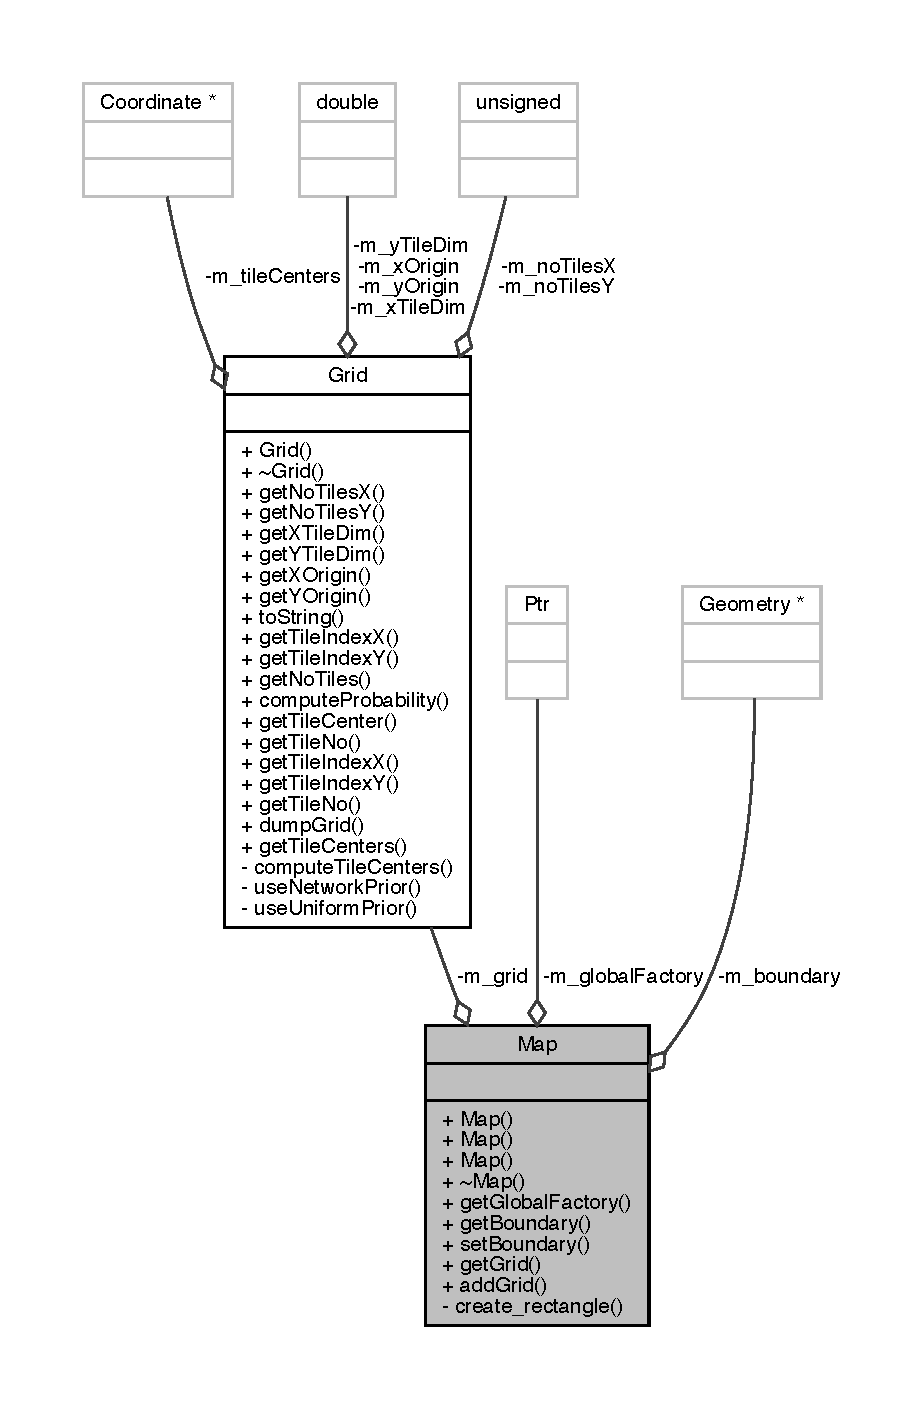
\includegraphics[width=350pt]{class_map__coll__graph}
\end{center}
\end{figure}
\subsection*{Public Member Functions}
\begin{DoxyCompactItemize}
\item 
\mbox{\hyperlink{class_map_a0f5ad0fd4563497b4214038cbca8b582}{Map}} ()
\item 
\mbox{\hyperlink{class_map_a4c9545a0252613e2a6808932fe83f9ad}{Map}} (double llX, double llY, double width, double height)
\item 
\mbox{\hyperlink{class_map_ab8beab7a7dce782a23db740cd7132552}{Map}} (string wkt\+File)
\item 
virtual \mbox{\hyperlink{class_map_ac1ab46138aa61acd0a58b1fd21e0df37}{$\sim$\+Map}} ()
\item 
const Geometry\+Factory\+::\+Ptr \& \mbox{\hyperlink{class_map_a69bd639b05daa393b051c76f0dc4af7c}{get\+Global\+Factory}} () const
\item 
Geometry $\ast$ \mbox{\hyperlink{class_map_a74dd5445ed90bea2a9cc3240bc23f1bc}{get\+Boundary}} () const
\item 
void \mbox{\hyperlink{class_map_acede2ccba9bf0f987f3dde8c332bec17}{set\+Boundary}} (Geometry $\ast$boundary)
\item 
const \mbox{\hyperlink{class_grid}{Grid}} $\ast$ \mbox{\hyperlink{class_map_aa9bf1c29b844f3b7fbf7a3153c24fef0}{get\+Grid}} () const
\item 
void \mbox{\hyperlink{class_map_aa3dba78a0b52b304c39d1fa6bff71b00}{add\+Grid}} (double dim\+TileX, double dim\+TileY)
\end{DoxyCompactItemize}
\subsection*{Private Member Functions}
\begin{DoxyCompactItemize}
\item 
Polygon $\ast$ \mbox{\hyperlink{class_map_a36539152d451138361d82469218b4661}{create\+\_\+rectangle}} (double llX, double llY, double width, double height)
\end{DoxyCompactItemize}
\subsection*{Private Attributes}
\begin{DoxyCompactItemize}
\item 
Geometry\+Factory\+::\+Ptr \mbox{\hyperlink{class_map_ac5f30e6c144955a3638192495fd7d843}{m\+\_\+global\+Factory}}
\item 
Geometry $\ast$ \mbox{\hyperlink{class_map_af2c95561cb4ff3b9950240351cf4303c}{m\+\_\+boundary}}
\item 
\mbox{\hyperlink{class_grid}{Grid}} $\ast$ \mbox{\hyperlink{class_map_a0fc16621dbe307d36170c3a96b24b7d9}{m\+\_\+grid}}
\end{DoxyCompactItemize}


\subsection{Detailed Description}
This is the map where the simulation takes place. It could be a simple rectangle or any kind of geometry object(s) read from a wkt file. The map has a boundary that is implemented as a Geometry object, a factory object of Geometry\+Factory type used to create other objects. All geometric and geographic features of the simulator uses the G\+E\+OS library. G\+E\+OS is an open source C++ library which is just a port to C++ of the well known Java Topology Suite. 

\subsection{Constructor \& Destructor Documentation}
\mbox{\Hypertarget{class_map_a0f5ad0fd4563497b4214038cbca8b582}\label{class_map_a0f5ad0fd4563497b4214038cbca8b582}} 
\index{Map@{Map}!Map@{Map}}
\index{Map@{Map}!Map@{Map}}
\subsubsection{\texorpdfstring{Map()}{Map()}\hspace{0.1cm}{\footnotesize\ttfamily [1/3]}}
{\footnotesize\ttfamily Map\+::\+Map (\begin{DoxyParamCaption}{ }\end{DoxyParamCaption})}

Creates a map with a null boundary. The user may set the boundary later, using \mbox{\hyperlink{class_map_acede2ccba9bf0f987f3dde8c332bec17}{set\+Boundary()}} method. \mbox{\Hypertarget{class_map_a4c9545a0252613e2a6808932fe83f9ad}\label{class_map_a4c9545a0252613e2a6808932fe83f9ad}} 
\index{Map@{Map}!Map@{Map}}
\index{Map@{Map}!Map@{Map}}
\subsubsection{\texorpdfstring{Map()}{Map()}\hspace{0.1cm}{\footnotesize\ttfamily [2/3]}}
{\footnotesize\ttfamily Map\+::\+Map (\begin{DoxyParamCaption}\item[{double}]{llX,  }\item[{double}]{llY,  }\item[{double}]{width,  }\item[{double}]{height }\end{DoxyParamCaption})}

Build a simple map of a rectangular shape. 
\begin{DoxyParams}{Parameters}
{\em llX} & X coordinate of the bottom left corner of the rectangle. \\
\hline
{\em llY} & Y coordinate of the bottom left corner of the rectangle. \\
\hline
{\em width} & the width of the rectangle. \\
\hline
{\em height} & the height of the rectangle. \\
\hline
\end{DoxyParams}
\mbox{\Hypertarget{class_map_ab8beab7a7dce782a23db740cd7132552}\label{class_map_ab8beab7a7dce782a23db740cd7132552}} 
\index{Map@{Map}!Map@{Map}}
\index{Map@{Map}!Map@{Map}}
\subsubsection{\texorpdfstring{Map()}{Map()}\hspace{0.1cm}{\footnotesize\ttfamily [3/3]}}
{\footnotesize\ttfamily Map\+::\+Map (\begin{DoxyParamCaption}\item[{string}]{wkt\+File }\end{DoxyParamCaption})}

Builds a map reading it from a .wkt file. 
\begin{DoxyParams}{Parameters}
{\em wkt\+File} & the name of the .wkt file that contains the description of the map. Currently, the first row of this file should contain the external boundary geometry of the map. \\
\hline
\end{DoxyParams}
\mbox{\Hypertarget{class_map_ac1ab46138aa61acd0a58b1fd21e0df37}\label{class_map_ac1ab46138aa61acd0a58b1fd21e0df37}} 
\index{Map@{Map}!````~Map@{$\sim$Map}}
\index{````~Map@{$\sim$Map}!Map@{Map}}
\subsubsection{\texorpdfstring{$\sim$Map()}{~Map()}}
{\footnotesize\ttfamily virtual Map\+::$\sim$\+Map (\begin{DoxyParamCaption}{ }\end{DoxyParamCaption})\hspace{0.3cm}{\ttfamily [virtual]}}

Default destructor 

\subsection{Member Function Documentation}
\mbox{\Hypertarget{class_map_aa3dba78a0b52b304c39d1fa6bff71b00}\label{class_map_aa3dba78a0b52b304c39d1fa6bff71b00}} 
\index{Map@{Map}!addGrid@{addGrid}}
\index{addGrid@{addGrid}!Map@{Map}}
\subsubsection{\texorpdfstring{addGrid()}{addGrid()}}
{\footnotesize\ttfamily void Map\+::add\+Grid (\begin{DoxyParamCaption}\item[{double}]{dim\+TileX,  }\item[{double}]{dim\+TileY }\end{DoxyParamCaption})}

Adds a \mbox{\hyperlink{class_grid}{Grid}} that overlaps this \mbox{\hyperlink{class_map}{Map}} objects. 
\begin{DoxyParams}{Parameters}
{\em dim\+TileX} & the dimension on OX of a tile of the \mbox{\hyperlink{class_grid}{Grid}} object. \\
\hline
{\em dim\+TileY} & the dimension on OY of a tile of the \mbox{\hyperlink{class_grid}{Grid}} object. \\
\hline
\end{DoxyParams}
\mbox{\Hypertarget{class_map_a36539152d451138361d82469218b4661}\label{class_map_a36539152d451138361d82469218b4661}} 
\index{Map@{Map}!create\_rectangle@{create\_rectangle}}
\index{create\_rectangle@{create\_rectangle}!Map@{Map}}
\subsubsection{\texorpdfstring{create\_rectangle()}{create\_rectangle()}}
{\footnotesize\ttfamily Polygon$\ast$ Map\+::create\+\_\+rectangle (\begin{DoxyParamCaption}\item[{double}]{llX,  }\item[{double}]{llY,  }\item[{double}]{width,  }\item[{double}]{height }\end{DoxyParamCaption})\hspace{0.3cm}{\ttfamily [private]}}

\mbox{\Hypertarget{class_map_a74dd5445ed90bea2a9cc3240bc23f1bc}\label{class_map_a74dd5445ed90bea2a9cc3240bc23f1bc}} 
\index{Map@{Map}!getBoundary@{getBoundary}}
\index{getBoundary@{getBoundary}!Map@{Map}}
\subsubsection{\texorpdfstring{getBoundary()}{getBoundary()}}
{\footnotesize\ttfamily Geometry$\ast$ Map\+::get\+Boundary (\begin{DoxyParamCaption}{ }\end{DoxyParamCaption}) const}

Returns a pointer to the Geometry object that represents the external boundary of the map. \begin{DoxyReturn}{Returns}
a pointer to the Geometry object that represents the external boundary of the map. 
\end{DoxyReturn}
\mbox{\Hypertarget{class_map_a69bd639b05daa393b051c76f0dc4af7c}\label{class_map_a69bd639b05daa393b051c76f0dc4af7c}} 
\index{Map@{Map}!getGlobalFactory@{getGlobalFactory}}
\index{getGlobalFactory@{getGlobalFactory}!Map@{Map}}
\subsubsection{\texorpdfstring{getGlobalFactory()}{getGlobalFactory()}}
{\footnotesize\ttfamily const Geometry\+Factory\+::\+Ptr\& Map\+::get\+Global\+Factory (\begin{DoxyParamCaption}{ }\end{DoxyParamCaption}) const}

Returns a pointer to the Geometry\+Factory object which is a factory object used to create other geometric objects. The G\+E\+OS library allows users to create geometric objects only using this factory, all the constructors are made private. \begin{DoxyReturn}{Returns}
a pointer to the Geometry\+Factory object used to create other geometric objects. 
\end{DoxyReturn}
\mbox{\Hypertarget{class_map_aa9bf1c29b844f3b7fbf7a3153c24fef0}\label{class_map_aa9bf1c29b844f3b7fbf7a3153c24fef0}} 
\index{Map@{Map}!getGrid@{getGrid}}
\index{getGrid@{getGrid}!Map@{Map}}
\subsubsection{\texorpdfstring{getGrid()}{getGrid()}}
{\footnotesize\ttfamily const \mbox{\hyperlink{class_grid}{Grid}}$\ast$ Map\+::get\+Grid (\begin{DoxyParamCaption}{ }\end{DoxyParamCaption}) const}

Returns a pointer to the \mbox{\hyperlink{class_grid}{Grid}} object associated with this \mbox{\hyperlink{class_map}{Map}}. After creation of a \mbox{\hyperlink{class_map}{Map}} the user should associate a \mbox{\hyperlink{class_grid}{Grid}} that overlaps this \mbox{\hyperlink{class_map}{Map}}. The gird is used to compute the probability of the localization of different events during the simulation. \begin{DoxyReturn}{Returns}
a pointer the \mbox{\hyperlink{class_grid}{Grid}} object associated with this \mbox{\hyperlink{class_map}{Map}}. 
\end{DoxyReturn}
\mbox{\Hypertarget{class_map_acede2ccba9bf0f987f3dde8c332bec17}\label{class_map_acede2ccba9bf0f987f3dde8c332bec17}} 
\index{Map@{Map}!setBoundary@{setBoundary}}
\index{setBoundary@{setBoundary}!Map@{Map}}
\subsubsection{\texorpdfstring{setBoundary()}{setBoundary()}}
{\footnotesize\ttfamily void Map\+::set\+Boundary (\begin{DoxyParamCaption}\item[{Geometry $\ast$}]{boundary }\end{DoxyParamCaption})}

Sets the boundary of the \mbox{\hyperlink{class_map}{Map}} object. 
\begin{DoxyParams}{Parameters}
{\em boundary} & the boundary of the \mbox{\hyperlink{class_map}{Map}} object. \\
\hline
\end{DoxyParams}


\subsection{Member Data Documentation}
\mbox{\Hypertarget{class_map_af2c95561cb4ff3b9950240351cf4303c}\label{class_map_af2c95561cb4ff3b9950240351cf4303c}} 
\index{Map@{Map}!m\_boundary@{m\_boundary}}
\index{m\_boundary@{m\_boundary}!Map@{Map}}
\subsubsection{\texorpdfstring{m\_boundary}{m\_boundary}}
{\footnotesize\ttfamily Geometry$\ast$ Map\+::m\+\_\+boundary\hspace{0.3cm}{\ttfamily [private]}}

\mbox{\Hypertarget{class_map_ac5f30e6c144955a3638192495fd7d843}\label{class_map_ac5f30e6c144955a3638192495fd7d843}} 
\index{Map@{Map}!m\_globalFactory@{m\_globalFactory}}
\index{m\_globalFactory@{m\_globalFactory}!Map@{Map}}
\subsubsection{\texorpdfstring{m\_globalFactory}{m\_globalFactory}}
{\footnotesize\ttfamily Geometry\+Factory\+::\+Ptr Map\+::m\+\_\+global\+Factory\hspace{0.3cm}{\ttfamily [private]}}

\mbox{\Hypertarget{class_map_a0fc16621dbe307d36170c3a96b24b7d9}\label{class_map_a0fc16621dbe307d36170c3a96b24b7d9}} 
\index{Map@{Map}!m\_grid@{m\_grid}}
\index{m\_grid@{m\_grid}!Map@{Map}}
\subsubsection{\texorpdfstring{m\_grid}{m\_grid}}
{\footnotesize\ttfamily \mbox{\hyperlink{class_grid}{Grid}}$\ast$ Map\+::m\+\_\+grid\hspace{0.3cm}{\ttfamily [private]}}



The documentation for this class was generated from the following file\+:\begin{DoxyCompactItemize}
\item 
include/\mbox{\hyperlink{_map_8h}{Map.\+h}}\end{DoxyCompactItemize}

\section{tinyxml2\+::Mem\+Pool Class Reference}
\label{classtinyxml2_1_1_mem_pool}\index{tinyxml2::MemPool@{tinyxml2::MemPool}}


{\ttfamily \#include $<$tinyxml2.\+h$>$}

Inheritance diagram for tinyxml2\+::Mem\+Pool\+:\begin{figure}[H]
\begin{center}
\leavevmode
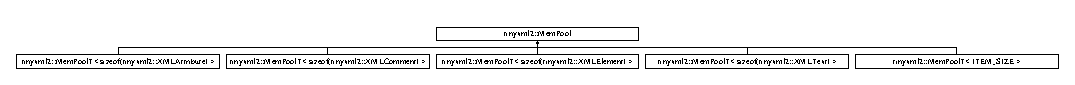
\includegraphics[height=0.691358cm]{classtinyxml2_1_1_mem_pool}
\end{center}
\end{figure}
\subsection*{Public Member Functions}
\begin{DoxyCompactItemize}
\item 
\textbf{ Mem\+Pool} ()
\item 
virtual \textbf{ $\sim$\+Mem\+Pool} ()
\item 
virtual int \textbf{ Item\+Size} () const =0
\item 
virtual void $\ast$ \textbf{ Alloc} ()=0
\item 
virtual void \textbf{ Free} (void $\ast$)=0
\item 
virtual void \textbf{ Set\+Tracked} ()=0
\end{DoxyCompactItemize}


\subsection{Detailed Description}


Definition at line 329 of file tinyxml2.\+h.



\subsection{Constructor \& Destructor Documentation}
\mbox{\label{classtinyxml2_1_1_mem_pool_a9101a0083d7370c85bd5aaaba7157f84}} 
\index{tinyxml2::MemPool@{tinyxml2::MemPool}!MemPool@{MemPool}}
\index{MemPool@{MemPool}!tinyxml2::MemPool@{tinyxml2::MemPool}}
\subsubsection{MemPool()}
{\footnotesize\ttfamily tinyxml2\+::\+Mem\+Pool\+::\+Mem\+Pool (\begin{DoxyParamCaption}{ }\end{DoxyParamCaption})\hspace{0.3cm}{\ttfamily [inline]}}



Definition at line 332 of file tinyxml2.\+h.

\mbox{\label{classtinyxml2_1_1_mem_pool_ae55ad9e3faeca702e6ccbb38fdbcad72}} 
\index{tinyxml2::MemPool@{tinyxml2::MemPool}!````~MemPool@{$\sim$MemPool}}
\index{````~MemPool@{$\sim$MemPool}!tinyxml2::MemPool@{tinyxml2::MemPool}}
\subsubsection{$\sim$MemPool()}
{\footnotesize\ttfamily virtual tinyxml2\+::\+Mem\+Pool\+::$\sim$\+Mem\+Pool (\begin{DoxyParamCaption}{ }\end{DoxyParamCaption})\hspace{0.3cm}{\ttfamily [inline]}, {\ttfamily [virtual]}}



Definition at line 333 of file tinyxml2.\+h.



\subsection{Member Function Documentation}
\mbox{\label{classtinyxml2_1_1_mem_pool_a4f977b5fed752c0bbfe5295f469d6449}} 
\index{tinyxml2::MemPool@{tinyxml2::MemPool}!Alloc@{Alloc}}
\index{Alloc@{Alloc}!tinyxml2::MemPool@{tinyxml2::MemPool}}
\subsubsection{Alloc()}
{\footnotesize\ttfamily virtual void$\ast$ tinyxml2\+::\+Mem\+Pool\+::\+Alloc (\begin{DoxyParamCaption}{ }\end{DoxyParamCaption})\hspace{0.3cm}{\ttfamily [pure virtual]}}



Implemented in \textbf{ tinyxml2\+::\+Mem\+Pool\+T$<$ I\+T\+E\+M\+\_\+\+S\+I\+Z\+E $>$} \doxyref{}{p.}{classtinyxml2_1_1_mem_pool_t_a810fd2b0caf56b8b688e55f2768f96c7}, \textbf{ tinyxml2\+::\+Mem\+Pool\+T$<$ sizeof(tinyxml2\+::\+X\+M\+L\+Comment) $>$} \doxyref{}{p.}{classtinyxml2_1_1_mem_pool_t_a810fd2b0caf56b8b688e55f2768f96c7}, \textbf{ tinyxml2\+::\+Mem\+Pool\+T$<$ sizeof(tinyxml2\+::\+X\+M\+L\+Text) $>$} \doxyref{}{p.}{classtinyxml2_1_1_mem_pool_t_a810fd2b0caf56b8b688e55f2768f96c7}, \textbf{ tinyxml2\+::\+Mem\+Pool\+T$<$ sizeof(tinyxml2\+::\+X\+M\+L\+Attribute) $>$} \doxyref{}{p.}{classtinyxml2_1_1_mem_pool_t_a810fd2b0caf56b8b688e55f2768f96c7}, and \textbf{ tinyxml2\+::\+Mem\+Pool\+T$<$ sizeof(tinyxml2\+::\+X\+M\+L\+Element) $>$} \doxyref{}{p.}{classtinyxml2_1_1_mem_pool_t_a810fd2b0caf56b8b688e55f2768f96c7}.

\mbox{\label{classtinyxml2_1_1_mem_pool_a49e3bfac2cba2ebd6776b31e571f64f7}} 
\index{tinyxml2::MemPool@{tinyxml2::MemPool}!Free@{Free}}
\index{Free@{Free}!tinyxml2::MemPool@{tinyxml2::MemPool}}
\subsubsection{Free()}
{\footnotesize\ttfamily virtual void tinyxml2\+::\+Mem\+Pool\+::\+Free (\begin{DoxyParamCaption}\item[{void $\ast$}]{ }\end{DoxyParamCaption})\hspace{0.3cm}{\ttfamily [pure virtual]}}



Implemented in \textbf{ tinyxml2\+::\+Mem\+Pool\+T$<$ I\+T\+E\+M\+\_\+\+S\+I\+Z\+E $>$} \doxyref{}{p.}{classtinyxml2_1_1_mem_pool_t_a408ce0918e9d3d5e5e1cc4896944875f}, \textbf{ tinyxml2\+::\+Mem\+Pool\+T$<$ sizeof(tinyxml2\+::\+X\+M\+L\+Comment) $>$} \doxyref{}{p.}{classtinyxml2_1_1_mem_pool_t_a408ce0918e9d3d5e5e1cc4896944875f}, \textbf{ tinyxml2\+::\+Mem\+Pool\+T$<$ sizeof(tinyxml2\+::\+X\+M\+L\+Text) $>$} \doxyref{}{p.}{classtinyxml2_1_1_mem_pool_t_a408ce0918e9d3d5e5e1cc4896944875f}, \textbf{ tinyxml2\+::\+Mem\+Pool\+T$<$ sizeof(tinyxml2\+::\+X\+M\+L\+Attribute) $>$} \doxyref{}{p.}{classtinyxml2_1_1_mem_pool_t_a408ce0918e9d3d5e5e1cc4896944875f}, and \textbf{ tinyxml2\+::\+Mem\+Pool\+T$<$ sizeof(tinyxml2\+::\+X\+M\+L\+Element) $>$} \doxyref{}{p.}{classtinyxml2_1_1_mem_pool_t_a408ce0918e9d3d5e5e1cc4896944875f}.



Referenced by tinyxml2\+::\+X\+M\+L\+Element\+::\+Delete\+Attribute(), and tinyxml2\+::\+X\+M\+L\+Node\+::\+Delete\+Node().

\mbox{\label{classtinyxml2_1_1_mem_pool_a0c518d49e3a94bde566f61e13b7240bb}} 
\index{tinyxml2::MemPool@{tinyxml2::MemPool}!ItemSize@{ItemSize}}
\index{ItemSize@{ItemSize}!tinyxml2::MemPool@{tinyxml2::MemPool}}
\subsubsection{ItemSize()}
{\footnotesize\ttfamily virtual int tinyxml2\+::\+Mem\+Pool\+::\+Item\+Size (\begin{DoxyParamCaption}{ }\end{DoxyParamCaption}) const\hspace{0.3cm}{\ttfamily [pure virtual]}}



Implemented in \textbf{ tinyxml2\+::\+Mem\+Pool\+T$<$ I\+T\+E\+M\+\_\+\+S\+I\+Z\+E $>$} \doxyref{}{p.}{classtinyxml2_1_1_mem_pool_t_a54e4d9b343459ef1731314a99877ff35}, \textbf{ tinyxml2\+::\+Mem\+Pool\+T$<$ sizeof(tinyxml2\+::\+X\+M\+L\+Comment) $>$} \doxyref{}{p.}{classtinyxml2_1_1_mem_pool_t_a54e4d9b343459ef1731314a99877ff35}, \textbf{ tinyxml2\+::\+Mem\+Pool\+T$<$ sizeof(tinyxml2\+::\+X\+M\+L\+Text) $>$} \doxyref{}{p.}{classtinyxml2_1_1_mem_pool_t_a54e4d9b343459ef1731314a99877ff35}, \textbf{ tinyxml2\+::\+Mem\+Pool\+T$<$ sizeof(tinyxml2\+::\+X\+M\+L\+Attribute) $>$} \doxyref{}{p.}{classtinyxml2_1_1_mem_pool_t_a54e4d9b343459ef1731314a99877ff35}, and \textbf{ tinyxml2\+::\+Mem\+Pool\+T$<$ sizeof(tinyxml2\+::\+X\+M\+L\+Element) $>$} \doxyref{}{p.}{classtinyxml2_1_1_mem_pool_t_a54e4d9b343459ef1731314a99877ff35}.

\mbox{\label{classtinyxml2_1_1_mem_pool_ac5804dd1387b2e4de5eef710076a0db1}} 
\index{tinyxml2::MemPool@{tinyxml2::MemPool}!SetTracked@{SetTracked}}
\index{SetTracked@{SetTracked}!tinyxml2::MemPool@{tinyxml2::MemPool}}
\subsubsection{SetTracked()}
{\footnotesize\ttfamily virtual void tinyxml2\+::\+Mem\+Pool\+::\+Set\+Tracked (\begin{DoxyParamCaption}{ }\end{DoxyParamCaption})\hspace{0.3cm}{\ttfamily [pure virtual]}}



Implemented in \textbf{ tinyxml2\+::\+Mem\+Pool\+T$<$ I\+T\+E\+M\+\_\+\+S\+I\+Z\+E $>$} \doxyref{}{p.}{classtinyxml2_1_1_mem_pool_t_aee3c611215ae08cce41a940bf2763027}, \textbf{ tinyxml2\+::\+Mem\+Pool\+T$<$ sizeof(tinyxml2\+::\+X\+M\+L\+Comment) $>$} \doxyref{}{p.}{classtinyxml2_1_1_mem_pool_t_aee3c611215ae08cce41a940bf2763027}, \textbf{ tinyxml2\+::\+Mem\+Pool\+T$<$ sizeof(tinyxml2\+::\+X\+M\+L\+Text) $>$} \doxyref{}{p.}{classtinyxml2_1_1_mem_pool_t_aee3c611215ae08cce41a940bf2763027}, \textbf{ tinyxml2\+::\+Mem\+Pool\+T$<$ sizeof(tinyxml2\+::\+X\+M\+L\+Attribute) $>$} \doxyref{}{p.}{classtinyxml2_1_1_mem_pool_t_aee3c611215ae08cce41a940bf2763027}, and \textbf{ tinyxml2\+::\+Mem\+Pool\+T$<$ sizeof(tinyxml2\+::\+X\+M\+L\+Element) $>$} \doxyref{}{p.}{classtinyxml2_1_1_mem_pool_t_aee3c611215ae08cce41a940bf2763027}.



Referenced by tinyxml2\+::\+X\+M\+L\+Document\+::\+Delete\+Node(), tinyxml2\+::\+X\+M\+L\+Node\+::\+Insert\+Child\+Preamble(), and tinyxml2\+::\+X\+M\+L\+Node\+::\+Parse\+Deep().



The documentation for this class was generated from the following file\+:\begin{DoxyCompactItemize}
\item 
include/\textbf{ tinyxml2.\+h}\end{DoxyCompactItemize}

\section{tinyxml2\+::Mem\+PoolT$<$ I\+T\+E\+M\+\_\+\+S\+I\+ZE $>$ Class Template Reference}
\label{classtinyxml2_1_1_mem_pool_t}\index{tinyxml2::MemPoolT$<$ ITEM\_SIZE $>$@{tinyxml2::MemPoolT$<$ ITEM\_SIZE $>$}}


{\ttfamily \#include $<$tinyxml2.\+h$>$}

Inheritance diagram for tinyxml2\+::Mem\+PoolT$<$ I\+T\+E\+M\+\_\+\+S\+I\+ZE $>$\+:\begin{figure}[H]
\begin{center}
\leavevmode
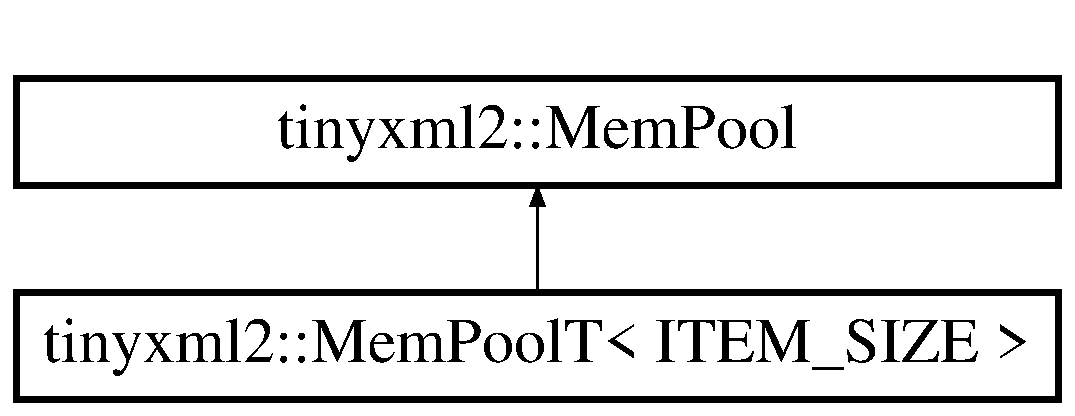
\includegraphics[height=2.000000cm]{classtinyxml2_1_1_mem_pool_t}
\end{center}
\end{figure}
\subsection*{Classes}
\begin{DoxyCompactItemize}
\item 
struct \textbf{ Block}
\item 
union \textbf{ Item}
\end{DoxyCompactItemize}
\subsection*{Public Types}
\begin{DoxyCompactItemize}
\item 
enum \{ \textbf{ I\+T\+E\+M\+S\+\_\+\+P\+E\+R\+\_\+\+B\+L\+O\+CK} = (4 $\ast$ 1024) / I\+T\+E\+M\+\_\+\+S\+I\+ZE
 \}
\end{DoxyCompactItemize}
\subsection*{Public Member Functions}
\begin{DoxyCompactItemize}
\item 
\textbf{ Mem\+PoolT} ()
\item 
\textbf{ $\sim$\+Mem\+PoolT} ()
\item 
void \textbf{ Clear} ()
\item 
virtual int \textbf{ Item\+Size} () const
\item 
int \textbf{ Current\+Allocs} () const
\item 
virtual void $\ast$ \textbf{ Alloc} ()
\item 
virtual void \textbf{ Free} (void $\ast$mem)
\item 
void \textbf{ Trace} (const char $\ast$name)
\item 
void \textbf{ Set\+Tracked} ()
\item 
int \textbf{ Untracked} () const
\end{DoxyCompactItemize}
\subsection*{Private Member Functions}
\begin{DoxyCompactItemize}
\item 
\textbf{ Mem\+PoolT} (const \textbf{ Mem\+PoolT} \&)
\item 
void \textbf{ operator=} (const \textbf{ Mem\+PoolT} \&)
\end{DoxyCompactItemize}
\subsection*{Private Attributes}
\begin{DoxyCompactItemize}
\item 
\textbf{ Dyn\+Array}$<$ \textbf{ Block} $\ast$, 10 $>$ \textbf{ \+\_\+block\+Ptrs}
\item 
\textbf{ Item} $\ast$ \textbf{ \+\_\+root}
\item 
int \textbf{ \+\_\+current\+Allocs}
\item 
int \textbf{ \+\_\+n\+Allocs}
\item 
int \textbf{ \+\_\+max\+Allocs}
\item 
int \textbf{ \+\_\+n\+Untracked}
\end{DoxyCompactItemize}


\subsection{Detailed Description}
\subsubsection*{template$<$int I\+T\+E\+M\+\_\+\+S\+I\+ZE$>$\newline
class tinyxml2\+::\+Mem\+Pool\+T$<$ I\+T\+E\+M\+\_\+\+S\+I\+Z\+E $>$}



Definition at line 346 of file tinyxml2.\+h.



\subsection{Member Enumeration Documentation}
\mbox{\label{classtinyxml2_1_1_mem_pool_t_a04cf45156e6f913f93972869ff8a1d94}} 
\subsubsection{anonymous enum}
{\footnotesize\ttfamily template$<$int I\+T\+E\+M\+\_\+\+S\+I\+ZE$>$ \\
anonymous enum}

\begin{DoxyEnumFields}{Enumerator}
\raisebox{\heightof{T}}[0pt][0pt]{\index{ITEMS\_PER\_BLOCK@{ITEMS\_PER\_BLOCK}!tinyxml2::MemPoolT$<$ ITEM\_SIZE $>$@{tinyxml2::MemPoolT$<$ ITEM\_SIZE $>$}}\index{tinyxml2::MemPoolT$<$ ITEM\_SIZE $>$@{tinyxml2::MemPoolT$<$ ITEM\_SIZE $>$}!ITEMS\_PER\_BLOCK@{ITEMS\_PER\_BLOCK}}}\mbox{\label{classtinyxml2_1_1_mem_pool_t_a04cf45156e6f913f93972869ff8a1d94ab72c1e16d6626854c41feb19e60c54d1}} 
I\+T\+E\+M\+S\+\_\+\+P\+E\+R\+\_\+\+B\+L\+O\+CK&\\
\hline

\end{DoxyEnumFields}


Definition at line 437 of file tinyxml2.\+h.



\subsection{Constructor \& Destructor Documentation}
\mbox{\label{classtinyxml2_1_1_mem_pool_t_ac8fa6dbb403f009cf9c8a33c6f2803b3}} 
\index{tinyxml2::MemPoolT$<$ ITEM\_SIZE $>$@{tinyxml2::MemPoolT$<$ ITEM\_SIZE $>$}!MemPoolT@{MemPoolT}}
\index{MemPoolT@{MemPoolT}!tinyxml2::MemPoolT$<$ ITEM\_SIZE $>$@{tinyxml2::MemPoolT$<$ ITEM\_SIZE $>$}}
\subsubsection{MemPoolT()\hspace{0.1cm}{\footnotesize\ttfamily [1/2]}}
{\footnotesize\ttfamily template$<$int I\+T\+E\+M\+\_\+\+S\+I\+ZE$>$ \\
\textbf{ tinyxml2\+::\+Mem\+PoolT}$<$ I\+T\+E\+M\+\_\+\+S\+I\+ZE $>$\+::\textbf{ Mem\+PoolT} (\begin{DoxyParamCaption}{ }\end{DoxyParamCaption})\hspace{0.3cm}{\ttfamily [inline]}}



Definition at line 349 of file tinyxml2.\+h.

\mbox{\label{classtinyxml2_1_1_mem_pool_t_a5fa4fee934a3df2b9e74282244d78390}} 
\index{tinyxml2::MemPoolT$<$ ITEM\_SIZE $>$@{tinyxml2::MemPoolT$<$ ITEM\_SIZE $>$}!````~MemPoolT@{$\sim$MemPoolT}}
\index{````~MemPoolT@{$\sim$MemPoolT}!tinyxml2::MemPoolT$<$ ITEM\_SIZE $>$@{tinyxml2::MemPoolT$<$ ITEM\_SIZE $>$}}
\subsubsection{$\sim$MemPoolT()}
{\footnotesize\ttfamily template$<$int I\+T\+E\+M\+\_\+\+S\+I\+ZE$>$ \\
\textbf{ tinyxml2\+::\+Mem\+PoolT}$<$ I\+T\+E\+M\+\_\+\+S\+I\+ZE $>$\+::$\sim$\textbf{ Mem\+PoolT} (\begin{DoxyParamCaption}{ }\end{DoxyParamCaption})\hspace{0.3cm}{\ttfamily [inline]}}



Definition at line 350 of file tinyxml2.\+h.

\mbox{\label{classtinyxml2_1_1_mem_pool_t_afa8770a0645d28bd849e7e5aefb326ed}} 
\index{tinyxml2::MemPoolT$<$ ITEM\_SIZE $>$@{tinyxml2::MemPoolT$<$ ITEM\_SIZE $>$}!MemPoolT@{MemPoolT}}
\index{MemPoolT@{MemPoolT}!tinyxml2::MemPoolT$<$ ITEM\_SIZE $>$@{tinyxml2::MemPoolT$<$ ITEM\_SIZE $>$}}
\subsubsection{MemPoolT()\hspace{0.1cm}{\footnotesize\ttfamily [2/2]}}
{\footnotesize\ttfamily template$<$int I\+T\+E\+M\+\_\+\+S\+I\+ZE$>$ \\
\textbf{ tinyxml2\+::\+Mem\+PoolT}$<$ I\+T\+E\+M\+\_\+\+S\+I\+ZE $>$\+::\textbf{ Mem\+PoolT} (\begin{DoxyParamCaption}\item[{const \textbf{ Mem\+PoolT}$<$ I\+T\+E\+M\+\_\+\+S\+I\+ZE $>$ \&}]{ }\end{DoxyParamCaption})\hspace{0.3cm}{\ttfamily [private]}}



\subsection{Member Function Documentation}
\mbox{\label{classtinyxml2_1_1_mem_pool_t_a810fd2b0caf56b8b688e55f2768f96c7}} 
\index{tinyxml2::MemPoolT$<$ ITEM\_SIZE $>$@{tinyxml2::MemPoolT$<$ ITEM\_SIZE $>$}!Alloc@{Alloc}}
\index{Alloc@{Alloc}!tinyxml2::MemPoolT$<$ ITEM\_SIZE $>$@{tinyxml2::MemPoolT$<$ ITEM\_SIZE $>$}}
\subsubsection{Alloc()}
{\footnotesize\ttfamily template$<$int I\+T\+E\+M\+\_\+\+S\+I\+ZE$>$ \\
virtual void$\ast$ \textbf{ tinyxml2\+::\+Mem\+PoolT}$<$ I\+T\+E\+M\+\_\+\+S\+I\+ZE $>$\+::Alloc (\begin{DoxyParamCaption}{ }\end{DoxyParamCaption})\hspace{0.3cm}{\ttfamily [inline]}, {\ttfamily [virtual]}}



Implements \textbf{ tinyxml2\+::\+Mem\+Pool} \doxyref{}{p.}{classtinyxml2_1_1_mem_pool_a4f977b5fed752c0bbfe5295f469d6449}.



Definition at line 374 of file tinyxml2.\+h.



Referenced by tinyxml2\+::\+X\+M\+L\+Document\+::\+Create\+Unlinked\+Node().

\mbox{\label{classtinyxml2_1_1_mem_pool_t_a22d595caa0e9d23aa080f49ca6475fdd}} 
\index{tinyxml2::MemPoolT$<$ ITEM\_SIZE $>$@{tinyxml2::MemPoolT$<$ ITEM\_SIZE $>$}!Clear@{Clear}}
\index{Clear@{Clear}!tinyxml2::MemPoolT$<$ ITEM\_SIZE $>$@{tinyxml2::MemPoolT$<$ ITEM\_SIZE $>$}}
\subsubsection{Clear()}
{\footnotesize\ttfamily template$<$int I\+T\+E\+M\+\_\+\+S\+I\+ZE$>$ \\
void \textbf{ tinyxml2\+::\+Mem\+PoolT}$<$ I\+T\+E\+M\+\_\+\+S\+I\+ZE $>$\+::Clear (\begin{DoxyParamCaption}{ }\end{DoxyParamCaption})\hspace{0.3cm}{\ttfamily [inline]}}



Definition at line 354 of file tinyxml2.\+h.



Referenced by tinyxml2\+::\+Mem\+Pool\+T$<$ sizeof(tinyxml2\+::\+X\+M\+L\+Element) $>$\+::$\sim$\+Mem\+Pool\+T().

\mbox{\label{classtinyxml2_1_1_mem_pool_t_a445a6c80151ba6268b24ec62a7c84d74}} 
\index{tinyxml2::MemPoolT$<$ ITEM\_SIZE $>$@{tinyxml2::MemPoolT$<$ ITEM\_SIZE $>$}!CurrentAllocs@{CurrentAllocs}}
\index{CurrentAllocs@{CurrentAllocs}!tinyxml2::MemPoolT$<$ ITEM\_SIZE $>$@{tinyxml2::MemPoolT$<$ ITEM\_SIZE $>$}}
\subsubsection{CurrentAllocs()}
{\footnotesize\ttfamily template$<$int I\+T\+E\+M\+\_\+\+S\+I\+ZE$>$ \\
int \textbf{ tinyxml2\+::\+Mem\+PoolT}$<$ I\+T\+E\+M\+\_\+\+S\+I\+ZE $>$\+::Current\+Allocs (\begin{DoxyParamCaption}{ }\end{DoxyParamCaption}) const\hspace{0.3cm}{\ttfamily [inline]}}



Definition at line 370 of file tinyxml2.\+h.

\mbox{\label{classtinyxml2_1_1_mem_pool_t_a408ce0918e9d3d5e5e1cc4896944875f}} 
\index{tinyxml2::MemPoolT$<$ ITEM\_SIZE $>$@{tinyxml2::MemPoolT$<$ ITEM\_SIZE $>$}!Free@{Free}}
\index{Free@{Free}!tinyxml2::MemPoolT$<$ ITEM\_SIZE $>$@{tinyxml2::MemPoolT$<$ ITEM\_SIZE $>$}}
\subsubsection{Free()}
{\footnotesize\ttfamily template$<$int I\+T\+E\+M\+\_\+\+S\+I\+ZE$>$ \\
virtual void \textbf{ tinyxml2\+::\+Mem\+PoolT}$<$ I\+T\+E\+M\+\_\+\+S\+I\+ZE $>$\+::Free (\begin{DoxyParamCaption}\item[{void $\ast$}]{mem }\end{DoxyParamCaption})\hspace{0.3cm}{\ttfamily [inline]}, {\ttfamily [virtual]}}



Implements \textbf{ tinyxml2\+::\+Mem\+Pool} \doxyref{}{p.}{classtinyxml2_1_1_mem_pool_a49e3bfac2cba2ebd6776b31e571f64f7}.



Definition at line 400 of file tinyxml2.\+h.

\mbox{\label{classtinyxml2_1_1_mem_pool_t_a54e4d9b343459ef1731314a99877ff35}} 
\index{tinyxml2::MemPoolT$<$ ITEM\_SIZE $>$@{tinyxml2::MemPoolT$<$ ITEM\_SIZE $>$}!ItemSize@{ItemSize}}
\index{ItemSize@{ItemSize}!tinyxml2::MemPoolT$<$ ITEM\_SIZE $>$@{tinyxml2::MemPoolT$<$ ITEM\_SIZE $>$}}
\subsubsection{ItemSize()}
{\footnotesize\ttfamily template$<$int I\+T\+E\+M\+\_\+\+S\+I\+ZE$>$ \\
virtual int \textbf{ tinyxml2\+::\+Mem\+PoolT}$<$ I\+T\+E\+M\+\_\+\+S\+I\+ZE $>$\+::Item\+Size (\begin{DoxyParamCaption}{ }\end{DoxyParamCaption}) const\hspace{0.3cm}{\ttfamily [inline]}, {\ttfamily [virtual]}}



Implements \textbf{ tinyxml2\+::\+Mem\+Pool} \doxyref{}{p.}{classtinyxml2_1_1_mem_pool_a0c518d49e3a94bde566f61e13b7240bb}.



Definition at line 367 of file tinyxml2.\+h.



Referenced by tinyxml2\+::\+X\+M\+L\+Document\+::\+Create\+Unlinked\+Node().

\mbox{\label{classtinyxml2_1_1_mem_pool_t_a12ba6478e385244beb2ca3947879fd24}} 
\index{tinyxml2::MemPoolT$<$ ITEM\_SIZE $>$@{tinyxml2::MemPoolT$<$ ITEM\_SIZE $>$}!operator=@{operator=}}
\index{operator=@{operator=}!tinyxml2::MemPoolT$<$ ITEM\_SIZE $>$@{tinyxml2::MemPoolT$<$ ITEM\_SIZE $>$}}
\subsubsection{operator=()}
{\footnotesize\ttfamily template$<$int I\+T\+E\+M\+\_\+\+S\+I\+ZE$>$ \\
void \textbf{ tinyxml2\+::\+Mem\+PoolT}$<$ I\+T\+E\+M\+\_\+\+S\+I\+ZE $>$\+::operator= (\begin{DoxyParamCaption}\item[{const \textbf{ Mem\+PoolT}$<$ I\+T\+E\+M\+\_\+\+S\+I\+ZE $>$ \&}]{ }\end{DoxyParamCaption})\hspace{0.3cm}{\ttfamily [private]}}

\mbox{\label{classtinyxml2_1_1_mem_pool_t_aee3c611215ae08cce41a940bf2763027}} 
\index{tinyxml2::MemPoolT$<$ ITEM\_SIZE $>$@{tinyxml2::MemPoolT$<$ ITEM\_SIZE $>$}!SetTracked@{SetTracked}}
\index{SetTracked@{SetTracked}!tinyxml2::MemPoolT$<$ ITEM\_SIZE $>$@{tinyxml2::MemPoolT$<$ ITEM\_SIZE $>$}}
\subsubsection{SetTracked()}
{\footnotesize\ttfamily template$<$int I\+T\+E\+M\+\_\+\+S\+I\+ZE$>$ \\
void \textbf{ tinyxml2\+::\+Mem\+PoolT}$<$ I\+T\+E\+M\+\_\+\+S\+I\+ZE $>$\+::Set\+Tracked (\begin{DoxyParamCaption}{ }\end{DoxyParamCaption})\hspace{0.3cm}{\ttfamily [inline]}, {\ttfamily [virtual]}}



Implements \textbf{ tinyxml2\+::\+Mem\+Pool} \doxyref{}{p.}{classtinyxml2_1_1_mem_pool_ac5804dd1387b2e4de5eef710076a0db1}.



Definition at line 418 of file tinyxml2.\+h.

\mbox{\label{classtinyxml2_1_1_mem_pool_t_a47eefbd934ef70d973ea41d41ab5f239}} 
\index{tinyxml2::MemPoolT$<$ ITEM\_SIZE $>$@{tinyxml2::MemPoolT$<$ ITEM\_SIZE $>$}!Trace@{Trace}}
\index{Trace@{Trace}!tinyxml2::MemPoolT$<$ ITEM\_SIZE $>$@{tinyxml2::MemPoolT$<$ ITEM\_SIZE $>$}}
\subsubsection{Trace()}
{\footnotesize\ttfamily template$<$int I\+T\+E\+M\+\_\+\+S\+I\+ZE$>$ \\
void \textbf{ tinyxml2\+::\+Mem\+PoolT}$<$ I\+T\+E\+M\+\_\+\+S\+I\+ZE $>$\+::Trace (\begin{DoxyParamCaption}\item[{const char $\ast$}]{name }\end{DoxyParamCaption})\hspace{0.3cm}{\ttfamily [inline]}}



Definition at line 412 of file tinyxml2.\+h.

\mbox{\label{classtinyxml2_1_1_mem_pool_t_a3bcdc302ae15d2810e11192321a8f5f1}} 
\index{tinyxml2::MemPoolT$<$ ITEM\_SIZE $>$@{tinyxml2::MemPoolT$<$ ITEM\_SIZE $>$}!Untracked@{Untracked}}
\index{Untracked@{Untracked}!tinyxml2::MemPoolT$<$ ITEM\_SIZE $>$@{tinyxml2::MemPoolT$<$ ITEM\_SIZE $>$}}
\subsubsection{Untracked()}
{\footnotesize\ttfamily template$<$int I\+T\+E\+M\+\_\+\+S\+I\+ZE$>$ \\
int \textbf{ tinyxml2\+::\+Mem\+PoolT}$<$ I\+T\+E\+M\+\_\+\+S\+I\+ZE $>$\+::Untracked (\begin{DoxyParamCaption}{ }\end{DoxyParamCaption}) const\hspace{0.3cm}{\ttfamily [inline]}}



Definition at line 422 of file tinyxml2.\+h.



\subsection{Member Data Documentation}
\mbox{\label{classtinyxml2_1_1_mem_pool_t_a028d833de2bf5e6257b4b27a68702a84}} 
\index{tinyxml2::MemPoolT$<$ ITEM\_SIZE $>$@{tinyxml2::MemPoolT$<$ ITEM\_SIZE $>$}!\_blockPtrs@{\_blockPtrs}}
\index{\_blockPtrs@{\_blockPtrs}!tinyxml2::MemPoolT$<$ ITEM\_SIZE $>$@{tinyxml2::MemPoolT$<$ ITEM\_SIZE $>$}}
\subsubsection{\_blockPtrs}
{\footnotesize\ttfamily template$<$int I\+T\+E\+M\+\_\+\+S\+I\+ZE$>$ \\
\textbf{ Dyn\+Array}$<$ \textbf{ Block}$\ast$, 10 $>$ \textbf{ tinyxml2\+::\+Mem\+PoolT}$<$ I\+T\+E\+M\+\_\+\+S\+I\+ZE $>$\+::\+\_\+block\+Ptrs\hspace{0.3cm}{\ttfamily [private]}}



Definition at line 450 of file tinyxml2.\+h.



Referenced by tinyxml2\+::\+Mem\+Pool\+T$<$ sizeof(tinyxml2\+::\+X\+M\+L\+Element) $>$\+::\+Alloc(), tinyxml2\+::\+Mem\+Pool\+T$<$ sizeof(tinyxml2\+::\+X\+M\+L\+Element) $>$\+::\+Clear(), and tinyxml2\+::\+Mem\+Pool\+T$<$ sizeof(tinyxml2\+::\+X\+M\+L\+Element) $>$\+::\+Trace().

\mbox{\label{classtinyxml2_1_1_mem_pool_t_afa908fd62011c6e633d7af196d667e9d}} 
\index{tinyxml2::MemPoolT$<$ ITEM\_SIZE $>$@{tinyxml2::MemPoolT$<$ ITEM\_SIZE $>$}!\_currentAllocs@{\_currentAllocs}}
\index{\_currentAllocs@{\_currentAllocs}!tinyxml2::MemPoolT$<$ ITEM\_SIZE $>$@{tinyxml2::MemPoolT$<$ ITEM\_SIZE $>$}}
\subsubsection{\_currentAllocs}
{\footnotesize\ttfamily template$<$int I\+T\+E\+M\+\_\+\+S\+I\+ZE$>$ \\
int \textbf{ tinyxml2\+::\+Mem\+PoolT}$<$ I\+T\+E\+M\+\_\+\+S\+I\+ZE $>$\+::\+\_\+current\+Allocs\hspace{0.3cm}{\ttfamily [private]}}



Definition at line 453 of file tinyxml2.\+h.



Referenced by tinyxml2\+::\+Mem\+Pool\+T$<$ sizeof(tinyxml2\+::\+X\+M\+L\+Element) $>$\+::\+Alloc(), tinyxml2\+::\+Mem\+Pool\+T$<$ sizeof(tinyxml2\+::\+X\+M\+L\+Element) $>$\+::\+Clear(), tinyxml2\+::\+Mem\+Pool\+T$<$ sizeof(tinyxml2\+::\+X\+M\+L\+Element) $>$\+::\+Current\+Allocs(), tinyxml2\+::\+Mem\+Pool\+T$<$ sizeof(tinyxml2\+::\+X\+M\+L\+Element) $>$\+::\+Free(), and tinyxml2\+::\+Mem\+Pool\+T$<$ sizeof(tinyxml2\+::\+X\+M\+L\+Element) $>$\+::\+Trace().

\mbox{\label{classtinyxml2_1_1_mem_pool_t_aaf3960c9e30197aeb1c0af271c297db9}} 
\index{tinyxml2::MemPoolT$<$ ITEM\_SIZE $>$@{tinyxml2::MemPoolT$<$ ITEM\_SIZE $>$}!\_maxAllocs@{\_maxAllocs}}
\index{\_maxAllocs@{\_maxAllocs}!tinyxml2::MemPoolT$<$ ITEM\_SIZE $>$@{tinyxml2::MemPoolT$<$ ITEM\_SIZE $>$}}
\subsubsection{\_maxAllocs}
{\footnotesize\ttfamily template$<$int I\+T\+E\+M\+\_\+\+S\+I\+ZE$>$ \\
int \textbf{ tinyxml2\+::\+Mem\+PoolT}$<$ I\+T\+E\+M\+\_\+\+S\+I\+ZE $>$\+::\+\_\+max\+Allocs\hspace{0.3cm}{\ttfamily [private]}}



Definition at line 455 of file tinyxml2.\+h.



Referenced by tinyxml2\+::\+Mem\+Pool\+T$<$ sizeof(tinyxml2\+::\+X\+M\+L\+Element) $>$\+::\+Alloc(), tinyxml2\+::\+Mem\+Pool\+T$<$ sizeof(tinyxml2\+::\+X\+M\+L\+Element) $>$\+::\+Clear(), and tinyxml2\+::\+Mem\+Pool\+T$<$ sizeof(tinyxml2\+::\+X\+M\+L\+Element) $>$\+::\+Trace().

\mbox{\label{classtinyxml2_1_1_mem_pool_t_acd5867e06ad91a655f3c9f95ca163e9b}} 
\index{tinyxml2::MemPoolT$<$ ITEM\_SIZE $>$@{tinyxml2::MemPoolT$<$ ITEM\_SIZE $>$}!\_nAllocs@{\_nAllocs}}
\index{\_nAllocs@{\_nAllocs}!tinyxml2::MemPoolT$<$ ITEM\_SIZE $>$@{tinyxml2::MemPoolT$<$ ITEM\_SIZE $>$}}
\subsubsection{\_nAllocs}
{\footnotesize\ttfamily template$<$int I\+T\+E\+M\+\_\+\+S\+I\+ZE$>$ \\
int \textbf{ tinyxml2\+::\+Mem\+PoolT}$<$ I\+T\+E\+M\+\_\+\+S\+I\+ZE $>$\+::\+\_\+n\+Allocs\hspace{0.3cm}{\ttfamily [private]}}



Definition at line 454 of file tinyxml2.\+h.



Referenced by tinyxml2\+::\+Mem\+Pool\+T$<$ sizeof(tinyxml2\+::\+X\+M\+L\+Element) $>$\+::\+Alloc(), tinyxml2\+::\+Mem\+Pool\+T$<$ sizeof(tinyxml2\+::\+X\+M\+L\+Element) $>$\+::\+Clear(), and tinyxml2\+::\+Mem\+Pool\+T$<$ sizeof(tinyxml2\+::\+X\+M\+L\+Element) $>$\+::\+Trace().

\mbox{\label{classtinyxml2_1_1_mem_pool_t_a5048ad99f7350f7224b13cf85fbff151}} 
\index{tinyxml2::MemPoolT$<$ ITEM\_SIZE $>$@{tinyxml2::MemPoolT$<$ ITEM\_SIZE $>$}!\_nUntracked@{\_nUntracked}}
\index{\_nUntracked@{\_nUntracked}!tinyxml2::MemPoolT$<$ ITEM\_SIZE $>$@{tinyxml2::MemPoolT$<$ ITEM\_SIZE $>$}}
\subsubsection{\_nUntracked}
{\footnotesize\ttfamily template$<$int I\+T\+E\+M\+\_\+\+S\+I\+ZE$>$ \\
int \textbf{ tinyxml2\+::\+Mem\+PoolT}$<$ I\+T\+E\+M\+\_\+\+S\+I\+ZE $>$\+::\+\_\+n\+Untracked\hspace{0.3cm}{\ttfamily [private]}}



Definition at line 456 of file tinyxml2.\+h.



Referenced by tinyxml2\+::\+Mem\+Pool\+T$<$ sizeof(tinyxml2\+::\+X\+M\+L\+Element) $>$\+::\+Alloc(), tinyxml2\+::\+Mem\+Pool\+T$<$ sizeof(tinyxml2\+::\+X\+M\+L\+Element) $>$\+::\+Clear(), tinyxml2\+::\+Mem\+Pool\+T$<$ sizeof(tinyxml2\+::\+X\+M\+L\+Element) $>$\+::\+Set\+Tracked(), and tinyxml2\+::\+Mem\+Pool\+T$<$ sizeof(tinyxml2\+::\+X\+M\+L\+Element) $>$\+::\+Untracked().

\mbox{\label{classtinyxml2_1_1_mem_pool_t_aff60ad785be00814e442e53fb4462688}} 
\index{tinyxml2::MemPoolT$<$ ITEM\_SIZE $>$@{tinyxml2::MemPoolT$<$ ITEM\_SIZE $>$}!\_root@{\_root}}
\index{\_root@{\_root}!tinyxml2::MemPoolT$<$ ITEM\_SIZE $>$@{tinyxml2::MemPoolT$<$ ITEM\_SIZE $>$}}
\subsubsection{\_root}
{\footnotesize\ttfamily template$<$int I\+T\+E\+M\+\_\+\+S\+I\+ZE$>$ \\
\textbf{ Item}$\ast$ \textbf{ tinyxml2\+::\+Mem\+PoolT}$<$ I\+T\+E\+M\+\_\+\+S\+I\+ZE $>$\+::\+\_\+root\hspace{0.3cm}{\ttfamily [private]}}



Definition at line 451 of file tinyxml2.\+h.



Referenced by tinyxml2\+::\+Mem\+Pool\+T$<$ sizeof(tinyxml2\+::\+X\+M\+L\+Element) $>$\+::\+Alloc(), tinyxml2\+::\+Mem\+Pool\+T$<$ sizeof(tinyxml2\+::\+X\+M\+L\+Element) $>$\+::\+Clear(), and tinyxml2\+::\+Mem\+Pool\+T$<$ sizeof(tinyxml2\+::\+X\+M\+L\+Element) $>$\+::\+Free().



The documentation for this class was generated from the following file\+:\begin{DoxyCompactItemize}
\item 
include/\textbf{ tinyxml2.\+h}\end{DoxyCompactItemize}

\hypertarget{class_mobile_phone}{}\section{Mobile\+Phone Class Reference}
\label{class_mobile_phone}\index{MobilePhone@{MobilePhone}}


{\ttfamily \#include $<$Mobile\+Phone.\+h$>$}



Inheritance diagram for Mobile\+Phone\+:
\nopagebreak
\begin{figure}[H]
\begin{center}
\leavevmode
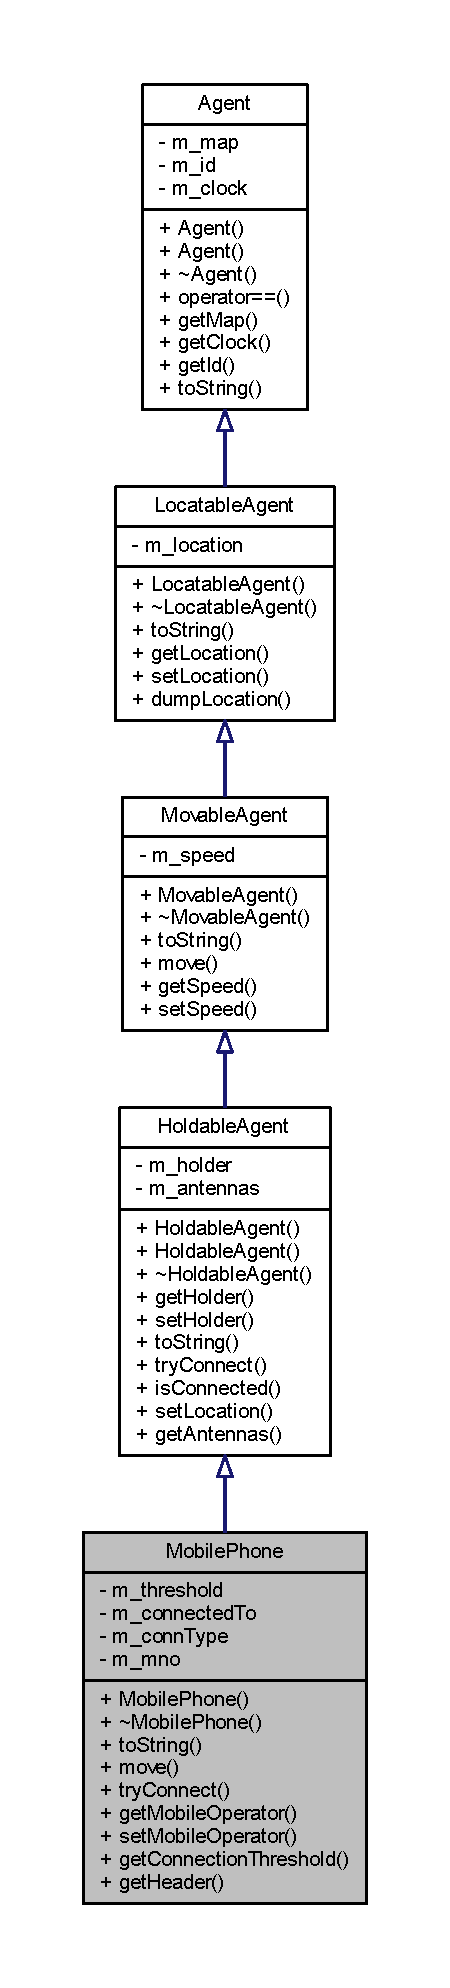
\includegraphics[height=550pt]{class_mobile_phone__inherit__graph}
\end{center}
\end{figure}


Collaboration diagram for Mobile\+Phone\+:
\nopagebreak
\begin{figure}[H]
\begin{center}
\leavevmode
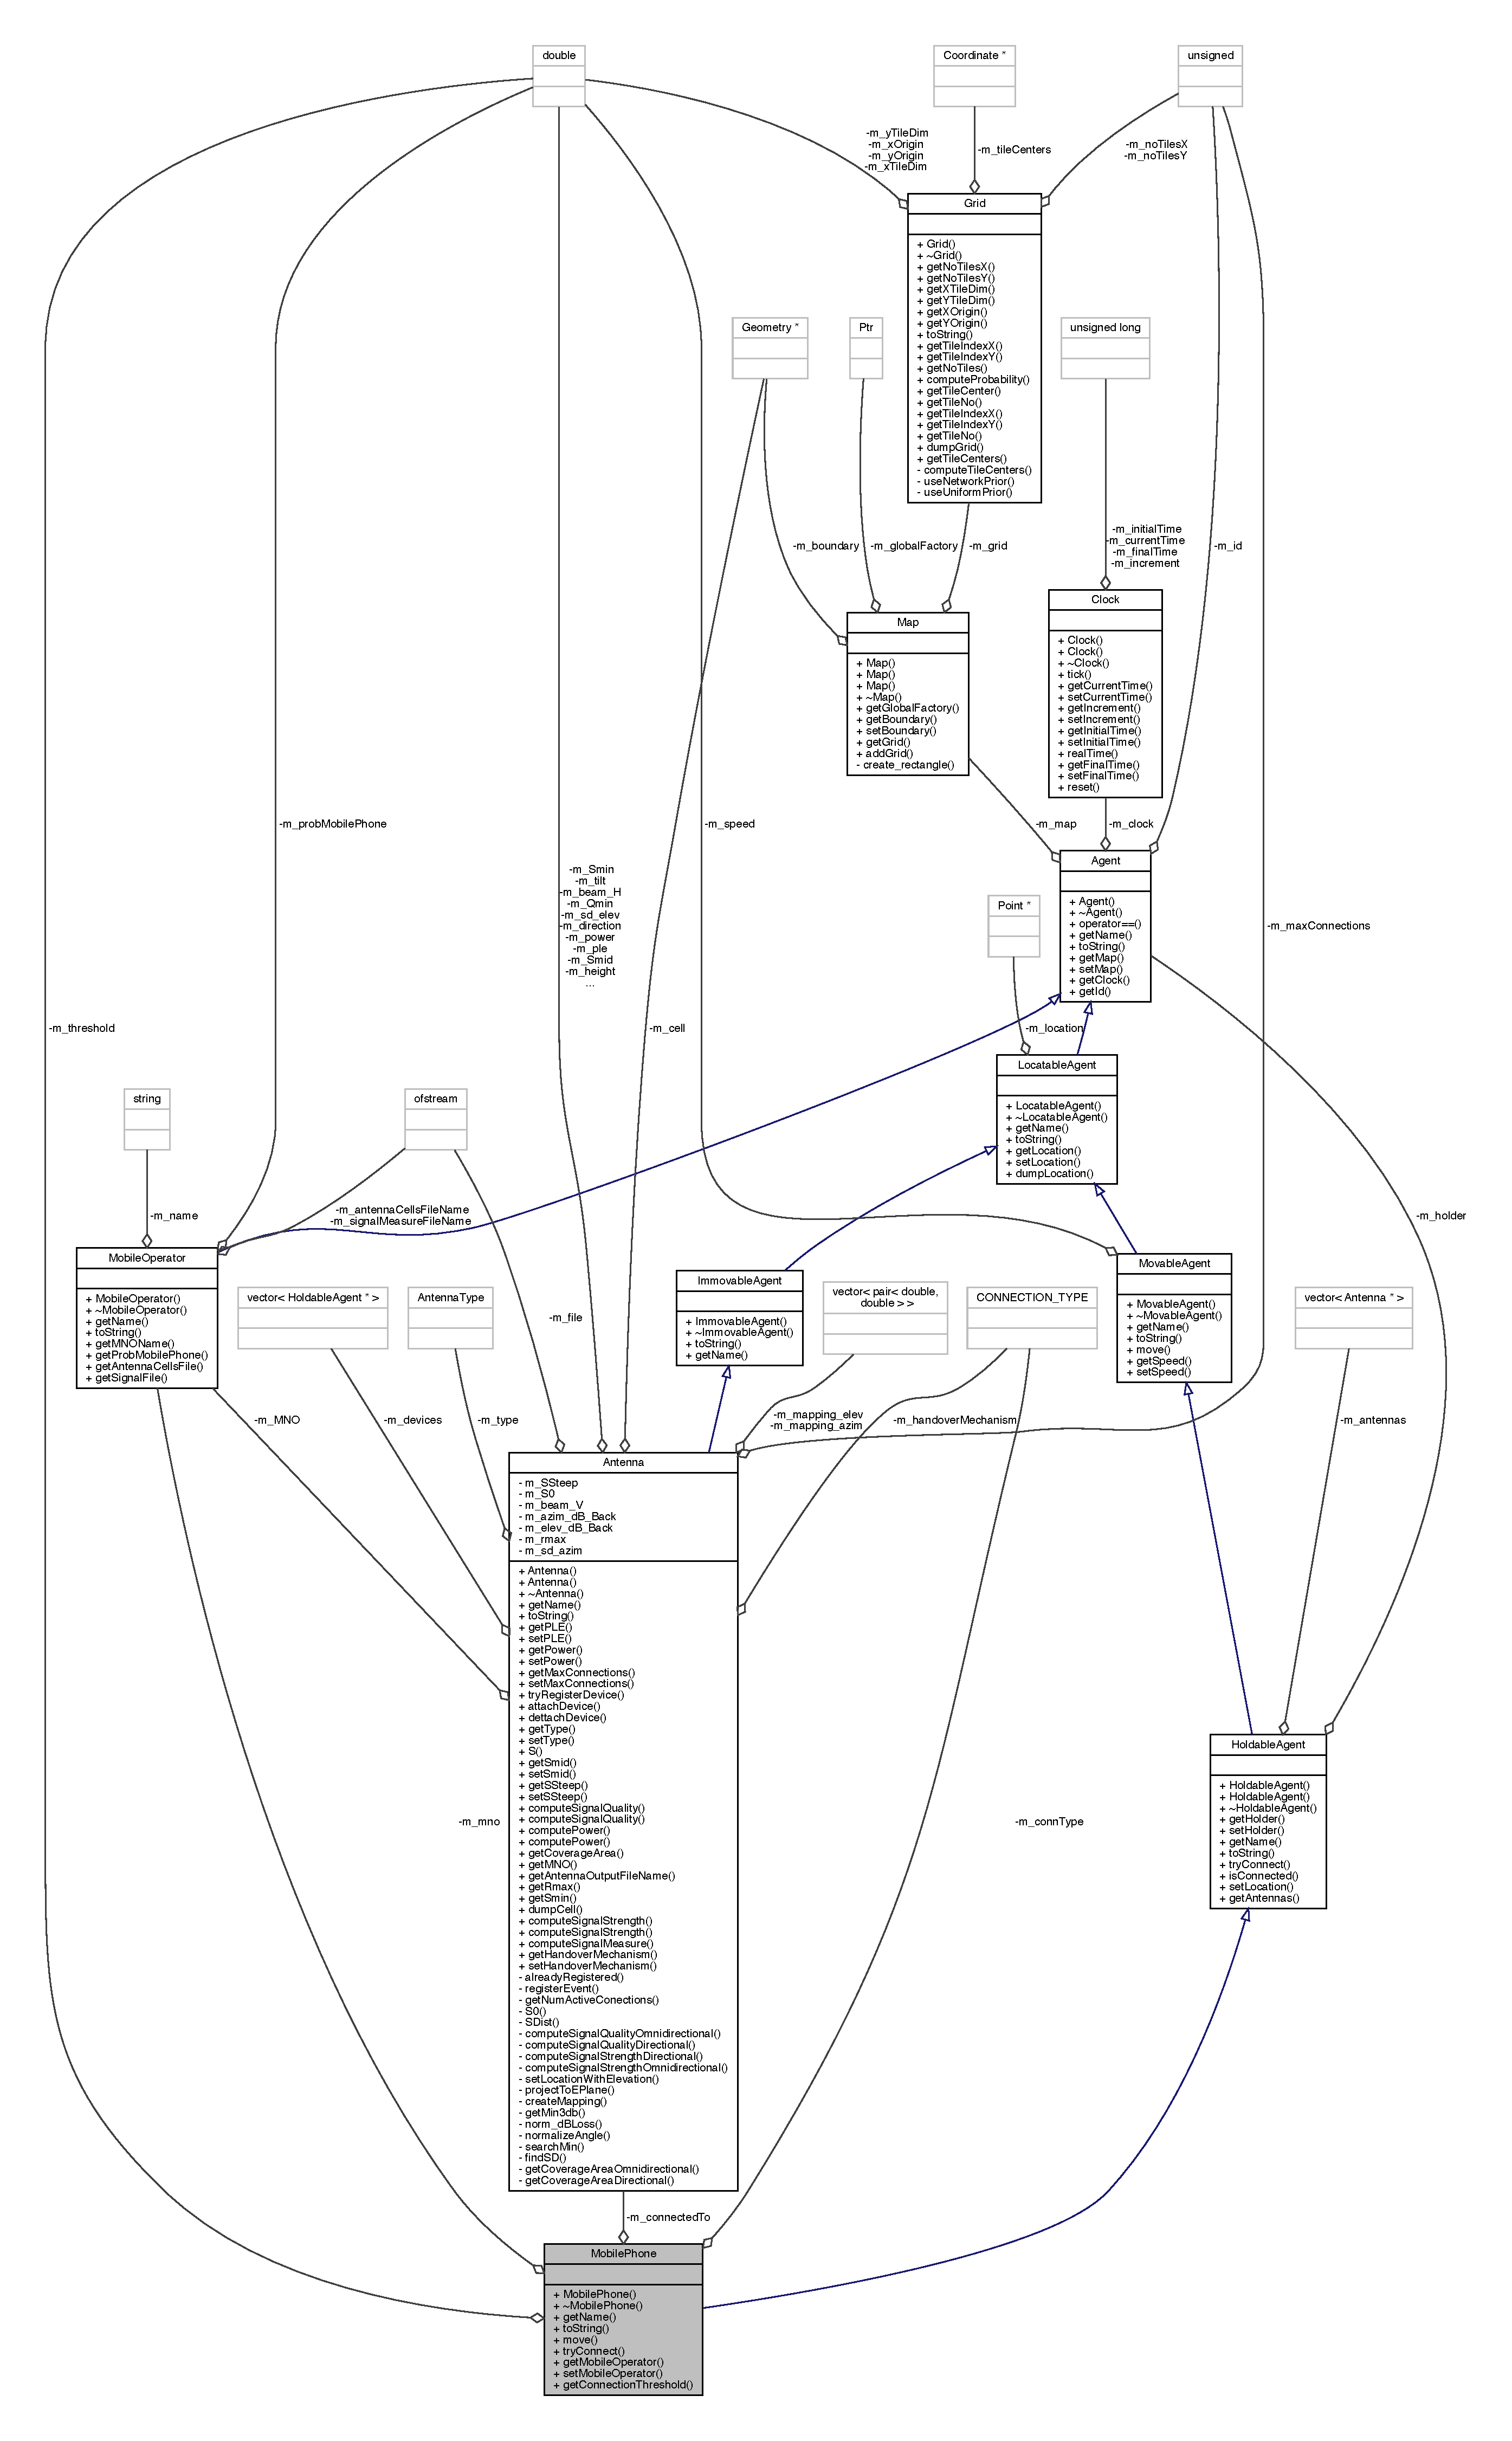
\includegraphics[height=550pt]{class_mobile_phone__coll__graph}
\end{center}
\end{figure}
\subsection*{Public Member Functions}
\begin{DoxyCompactItemize}
\item 
\mbox{\hyperlink{class_mobile_phone_afd7beed70eb2af3baecd9521332ba8eb}{Mobile\+Phone}} (const \mbox{\hyperlink{class_map}{Map}} $\ast$m, const unsigned long id, Point $\ast$init\+Position, \mbox{\hyperlink{class_agent}{Agent}} $\ast$holder, const \mbox{\hyperlink{class_clock}{Clock}} $\ast$clock, double threshold, \mbox{\hyperlink{class_holdable_agent_ae2c334b004d7b9c5a999cf2618e4e518}{Holdable\+Agent\+::\+C\+O\+N\+N\+E\+C\+T\+I\+O\+N\+\_\+\+T\+Y\+PE}} conn\+Type)
\item 
virtual \mbox{\hyperlink{class_mobile_phone_a51db1d9b4fcc52ea9f8d613dae4f6a4b}{$\sim$\+Mobile\+Phone}} ()
\item 
const string \mbox{\hyperlink{class_mobile_phone_a1eeac3141baafa75ebcf26fc3a0e4068}{get\+Name}} () const override
\item 
const string \mbox{\hyperlink{class_mobile_phone_a2b7e556d12a43e380786ad0eccf3ce04}{to\+String}} () const override
\item 
Point $\ast$ \mbox{\hyperlink{class_mobile_phone_a92d77fa5810ddb9c4c482d9c9baea456}{move}} (\mbox{\hyperlink{_movement_type_8h_a8a93b61bc797a7d1907f42796a252493}{Movement\+Type}} mv\+Type) override
\item 
bool \mbox{\hyperlink{class_mobile_phone_ad91afa811cea8ee124167f5941bcda1b}{try\+Connect}} () override
\item 
const \mbox{\hyperlink{class_mobile_operator}{Mobile\+Operator}} $\ast$ \mbox{\hyperlink{class_mobile_phone_aba72025d08c382d8533e0cbb9166999b}{get\+Mobile\+Operator}} () const
\item 
void \mbox{\hyperlink{class_mobile_phone_ad4db8203e8f2e974733357d7c3e6cf28}{set\+Mobile\+Operator}} (\mbox{\hyperlink{class_mobile_operator}{Mobile\+Operator}} $\ast$mno)
\item 
double \mbox{\hyperlink{class_mobile_phone_a57475711a8f85086f50067d219f1181d}{get\+Connection\+Threshold}} () const
\end{DoxyCompactItemize}
\subsection*{Private Attributes}
\begin{DoxyCompactItemize}
\item 
double \mbox{\hyperlink{class_mobile_phone_afb6364675f7cf6e09856f49ae6c10563}{m\+\_\+threshold}}
\item 
\mbox{\hyperlink{class_antenna}{Antenna}} $\ast$ \mbox{\hyperlink{class_mobile_phone_aa143b94346485788c3563228f6043721}{m\+\_\+connected\+To}}
\item 
\mbox{\hyperlink{class_holdable_agent_ae2c334b004d7b9c5a999cf2618e4e518}{Holdable\+Agent\+::\+C\+O\+N\+N\+E\+C\+T\+I\+O\+N\+\_\+\+T\+Y\+PE}} \mbox{\hyperlink{class_mobile_phone_a39f69fef45f380e3922dfe78b904372d}{m\+\_\+conn\+Type}}
\item 
\mbox{\hyperlink{class_mobile_operator}{Mobile\+Operator}} $\ast$ \mbox{\hyperlink{class_mobile_phone_a1b26abc840ac8f8679dd62939330c597}{m\+\_\+mno}}
\end{DoxyCompactItemize}
\subsection*{Additional Inherited Members}


\subsection{Detailed Description}
This class represents a mobile phone. A mobile phone is own by a \mbox{\hyperlink{class_person}{Person}} and it moves on the map together with its owner. While moving, at every time step it tries to connect to an antenna. The connection event is triggered by \mbox{\hyperlink{class_holdable_agent_aec98d2fe325b48d9a84ad3dad44700e0}{set\+Location()}}. The connection to antenna is determined by the signal emitted by antennas. A parameter in the simulation configuration file set the criterion used to connect\+: the power of the signal, the signal strength or the signal quality. 

\subsection{Constructor \& Destructor Documentation}
\mbox{\Hypertarget{class_mobile_phone_afd7beed70eb2af3baecd9521332ba8eb}\label{class_mobile_phone_afd7beed70eb2af3baecd9521332ba8eb}} 
\index{MobilePhone@{MobilePhone}!MobilePhone@{MobilePhone}}
\index{MobilePhone@{MobilePhone}!MobilePhone@{MobilePhone}}
\subsubsection{\texorpdfstring{MobilePhone()}{MobilePhone()}}
{\footnotesize\ttfamily Mobile\+Phone\+::\+Mobile\+Phone (\begin{DoxyParamCaption}\item[{const \mbox{\hyperlink{class_map}{Map}} $\ast$}]{m,  }\item[{const unsigned long}]{id,  }\item[{Point $\ast$}]{init\+Position,  }\item[{\mbox{\hyperlink{class_agent}{Agent}} $\ast$}]{holder,  }\item[{const \mbox{\hyperlink{class_clock}{Clock}} $\ast$}]{clock,  }\item[{double}]{threshold,  }\item[{\mbox{\hyperlink{class_holdable_agent_ae2c334b004d7b9c5a999cf2618e4e518}{Holdable\+Agent\+::\+C\+O\+N\+N\+E\+C\+T\+I\+O\+N\+\_\+\+T\+Y\+PE}}}]{conn\+Type }\end{DoxyParamCaption})\hspace{0.3cm}{\ttfamily [explicit]}}

Builds a new Mobilew\+Phone object with the parameters provided by the user. 
\begin{DoxyParams}{Parameters}
{\em m} & a pointer to the \mbox{\hyperlink{class_map}{Map}} object where the simulation takes place. \\
\hline
{\em id} & the id of the mobile phone. \\
\hline
{\em init\+Position} & the initial location of the phone on the map. \\
\hline
{\em holder} & a pointer to the \mbox{\hyperlink{class_agent}{Agent}} object that owns this mobile phone. \\
\hline
{\em clock} & a pointer to the \mbox{\hyperlink{class_clock}{Clock}} object used in this simulation. \\
\hline
{\em threshold} & the minimum power, signal qaulity or signal strength of the field below which the mobile phone cannot connect to an antenna. \\
\hline
{\em conn\+Type} & the criterion used for the connection to an antenna\+: based on the power of the signal or based on the signal quality. It could take three values\+: Holdable\+Agent\+::\+C\+O\+N\+N\+E\+C\+T\+I\+O\+N\+\_\+\+T\+Y\+P\+E\+::\+U\+S\+I\+N\+G\+\_\+\+P\+O\+W\+ER, Holdable\+Agent\+::\+C\+O\+N\+N\+E\+C\+T\+I\+O\+N\+\_\+\+T\+Y\+P\+E\+::\+U\+S\+I\+N\+G\+\_\+\+S\+I\+G\+N\+A\+L\+\_\+\+Q\+U\+A\+L\+I\+TY or Holdable\+Agent\+::\+C\+O\+N\+N\+E\+C\+T\+I\+O\+N\+\_\+\+T\+Y\+P\+E\+::\+U\+S\+I\+N\+G\+\_\+\+S\+I\+G\+N\+A\+L\+\_\+\+S\+T\+R\+E\+N\+G\+TH. \\
\hline
\end{DoxyParams}
\mbox{\Hypertarget{class_mobile_phone_a51db1d9b4fcc52ea9f8d613dae4f6a4b}\label{class_mobile_phone_a51db1d9b4fcc52ea9f8d613dae4f6a4b}} 
\index{MobilePhone@{MobilePhone}!````~MobilePhone@{$\sim$MobilePhone}}
\index{````~MobilePhone@{$\sim$MobilePhone}!MobilePhone@{MobilePhone}}
\subsubsection{\texorpdfstring{$\sim$MobilePhone()}{~MobilePhone()}}
{\footnotesize\ttfamily virtual Mobile\+Phone\+::$\sim$\+Mobile\+Phone (\begin{DoxyParamCaption}{ }\end{DoxyParamCaption})\hspace{0.3cm}{\ttfamily [virtual]}}

The default destructor. 

\subsection{Member Function Documentation}
\mbox{\Hypertarget{class_mobile_phone_a57475711a8f85086f50067d219f1181d}\label{class_mobile_phone_a57475711a8f85086f50067d219f1181d}} 
\index{MobilePhone@{MobilePhone}!getConnectionThreshold@{getConnectionThreshold}}
\index{getConnectionThreshold@{getConnectionThreshold}!MobilePhone@{MobilePhone}}
\subsubsection{\texorpdfstring{getConnectionThreshold()}{getConnectionThreshold()}}
{\footnotesize\ttfamily double Mobile\+Phone\+::get\+Connection\+Threshold (\begin{DoxyParamCaption}{ }\end{DoxyParamCaption}) const}

Returns the minimum value of the signal strength/power/quality below which the phone cannot use the signal (i.\+e. the signal is considered noise). The returned value is interpreted as signal strength, power or quality according to the connection type. \begin{DoxyReturn}{Returns}
the minimum value of the signal strength/power/quality below which the phone cannot use the signal (i.\+e. the signal is considered noise). 
\end{DoxyReturn}
\mbox{\Hypertarget{class_mobile_phone_aba72025d08c382d8533e0cbb9166999b}\label{class_mobile_phone_aba72025d08c382d8533e0cbb9166999b}} 
\index{MobilePhone@{MobilePhone}!getMobileOperator@{getMobileOperator}}
\index{getMobileOperator@{getMobileOperator}!MobilePhone@{MobilePhone}}
\subsubsection{\texorpdfstring{getMobileOperator()}{getMobileOperator()}}
{\footnotesize\ttfamily const \mbox{\hyperlink{class_mobile_operator}{Mobile\+Operator}}$\ast$ Mobile\+Phone\+::get\+Mobile\+Operator (\begin{DoxyParamCaption}{ }\end{DoxyParamCaption}) const}

Returns the \mbox{\hyperlink{class_mobile_operator}{Mobile\+Operator}} object of this mobile phone. Each \mbox{\hyperlink{class_mobile_phone}{Mobile\+Phone}} should belong to a Mobile Operator. \begin{DoxyReturn}{Returns}
the \mbox{\hyperlink{class_mobile_operator}{Mobile\+Operator}} object of this mobile phone. Each \mbox{\hyperlink{class_mobile_phone}{Mobile\+Phone}} should belong to a Mobile Operator. 
\end{DoxyReturn}
\mbox{\Hypertarget{class_mobile_phone_a1eeac3141baafa75ebcf26fc3a0e4068}\label{class_mobile_phone_a1eeac3141baafa75ebcf26fc3a0e4068}} 
\index{MobilePhone@{MobilePhone}!getName@{getName}}
\index{getName@{getName}!MobilePhone@{MobilePhone}}
\subsubsection{\texorpdfstring{getName()}{getName()}}
{\footnotesize\ttfamily const string Mobile\+Phone\+::get\+Name (\begin{DoxyParamCaption}{ }\end{DoxyParamCaption}) const\hspace{0.3cm}{\ttfamily [override]}, {\ttfamily [virtual]}}

Returns the name of this class. \begin{DoxyReturn}{Returns}
the name of this class. 
\end{DoxyReturn}


Reimplemented from \mbox{\hyperlink{class_holdable_agent_ab330bb40de51a957ef8826af629f94a2}{Holdable\+Agent}}.

\mbox{\Hypertarget{class_mobile_phone_a92d77fa5810ddb9c4c482d9c9baea456}\label{class_mobile_phone_a92d77fa5810ddb9c4c482d9c9baea456}} 
\index{MobilePhone@{MobilePhone}!move@{move}}
\index{move@{move}!MobilePhone@{MobilePhone}}
\subsubsection{\texorpdfstring{move()}{move()}}
{\footnotesize\ttfamily Point$\ast$ Mobile\+Phone\+::move (\begin{DoxyParamCaption}\item[{\mbox{\hyperlink{_movement_type_8h_a8a93b61bc797a7d1907f42796a252493}{Movement\+Type}}}]{mv\+Type }\end{DoxyParamCaption})\hspace{0.3cm}{\ttfamily [inline]}, {\ttfamily [override]}, {\ttfamily [virtual]}}

Makes a step on the map according to an algorithm. The direction and the length of the step is determined by the mv\+Type parameter and by the \mbox{\hyperlink{class_person}{Person}} object who owns this phone. 
\begin{DoxyParams}{Parameters}
{\em mv\+Type} & selects the way people and their phones are moving on the map. At this moment only R\+A\+N\+D\+O\+M\+\_\+\+W\+A\+L\+K\+\_\+\+C\+L\+O\+S\+E\+D\+\_\+\+M\+AP and R\+A\+N\+D\+O\+M\+\_\+\+W\+A\+L\+K\+\_\+\+C\+L\+O\+S\+E\+D\+\_\+\+M\+A\+P\+\_\+\+W\+I\+T\+H\+\_\+\+D\+R\+I\+FT are implemented. R\+A\+N\+D\+O\+M\+\_\+\+W\+A\+L\+K\+\_\+\+C\+L\+O\+S\+E\+D\+\_\+\+M\+AP means that at each time instant the direction is generated as a uniformly distributed random value and the step length is computed multiplying the speed with the time interval set in the simulation configuration file. If a step projects it outside the map, it stops on the boundary. \mbox{\hyperlink{_movement_type_8h_a8a93b61bc797a7d1907f42796a252493a19d5a14b0e46bf765f243b7e2b7b8810}{Movement\+Type\+::\+R\+A\+N\+D\+O\+M\+\_\+\+W\+A\+L\+K\+\_\+\+C\+L\+O\+S\+E\+D\+\_\+\+M\+A\+P\+\_\+\+W\+I\+T\+H\+\_\+\+D\+R\+I\+FT}} means that there is a preference in the direction of the movement. There are two constants defined, S\+I\+M\+\_\+\+T\+R\+E\+N\+D\+\_\+\+A\+N\+G\+L\+E\+\_\+1 and S\+I\+M\+\_\+\+T\+R\+E\+N\+D\+\_\+\+A\+N\+G\+L\+E\+\_\+2 (3P\+I/4 and 5P\+I/4), and in the first half of the simulation the direction is generated as a normal distributed random value with the mean equals to S\+I\+M\+\_\+\+T\+R\+E\+N\+D\+\_\+\+A\+N\+G\+L\+E\+\_\+1 and sd = 0.\+1 while during the second half of the simulation it is generated as a normal distributed random value with the mean equals to S\+I\+M\+\_\+\+T\+R\+E\+N\+D\+\_\+\+A\+N\+G\+L\+E\+\_\+2 and the same sd. Again, a \mbox{\hyperlink{class_movable_agent}{Movable\+Agent}} can only move inside the map boundary. If a step projects it outside the map, it stops on the boundary.\\
\hline
\end{DoxyParams}
\begin{DoxyReturn}{Returns}
the final location after the movement. 
\end{DoxyReturn}


Implements \mbox{\hyperlink{class_movable_agent_a35299e133c6787689b553d74ce5f98f0}{Movable\+Agent}}.

\mbox{\Hypertarget{class_mobile_phone_ad4db8203e8f2e974733357d7c3e6cf28}\label{class_mobile_phone_ad4db8203e8f2e974733357d7c3e6cf28}} 
\index{MobilePhone@{MobilePhone}!setMobileOperator@{setMobileOperator}}
\index{setMobileOperator@{setMobileOperator}!MobilePhone@{MobilePhone}}
\subsubsection{\texorpdfstring{setMobileOperator()}{setMobileOperator()}}
{\footnotesize\ttfamily void Mobile\+Phone\+::set\+Mobile\+Operator (\begin{DoxyParamCaption}\item[{\mbox{\hyperlink{class_mobile_operator}{Mobile\+Operator}} $\ast$}]{mno }\end{DoxyParamCaption})}

Sets the \mbox{\hyperlink{class_mobile_operator}{Mobile\+Operator}} object which owns this phone. 
\begin{DoxyParams}{Parameters}
{\em mno} & the \mbox{\hyperlink{class_mobile_operator}{Mobile\+Operator}} object which owns this phone. \\
\hline
\end{DoxyParams}
\mbox{\Hypertarget{class_mobile_phone_a2b7e556d12a43e380786ad0eccf3ce04}\label{class_mobile_phone_a2b7e556d12a43e380786ad0eccf3ce04}} 
\index{MobilePhone@{MobilePhone}!toString@{toString}}
\index{toString@{toString}!MobilePhone@{MobilePhone}}
\subsubsection{\texorpdfstring{toString()}{toString()}}
{\footnotesize\ttfamily const string Mobile\+Phone\+::to\+String (\begin{DoxyParamCaption}{ }\end{DoxyParamCaption}) const\hspace{0.3cm}{\ttfamily [override]}, {\ttfamily [virtual]}}

Returns a human readable string representation of this class useful to output it to a file or console. \begin{DoxyReturn}{Returns}
a human readable string representation of this class. 
\end{DoxyReturn}


Reimplemented from \mbox{\hyperlink{class_holdable_agent_a2c581226b8994f24b6b2306ae17dbb52}{Holdable\+Agent}}.

\mbox{\Hypertarget{class_mobile_phone_ad91afa811cea8ee124167f5941bcda1b}\label{class_mobile_phone_ad91afa811cea8ee124167f5941bcda1b}} 
\index{MobilePhone@{MobilePhone}!tryConnect@{tryConnect}}
\index{tryConnect@{tryConnect}!MobilePhone@{MobilePhone}}
\subsubsection{\texorpdfstring{tryConnect()}{tryConnect()}}
{\footnotesize\ttfamily bool Mobile\+Phone\+::try\+Connect (\begin{DoxyParamCaption}{ }\end{DoxyParamCaption})\hspace{0.3cm}{\ttfamily [override]}, {\ttfamily [virtual]}}

This method is called after the phone moves (together with its owner) to a new location. It tries to connect the mobile phone to an antenna. The connection method is determined by inspecting the m\+\_\+conn\+Type\+: using the power of the signal, using the quality of the signal or using the signal strength. The value of the m\+\_\+conn\+Type is set by the constructor of the class. If the connection is successfully a pointer to the \mbox{\hyperlink{class_antenna}{Antenna}} object where this mobile phone was connected is stored internally. \begin{DoxyReturn}{Returns}
true if the connection succeeds, false otherwise. 
\end{DoxyReturn}


Implements \mbox{\hyperlink{class_holdable_agent_a0789d757d81b43ee016e9362046f6dea}{Holdable\+Agent}}.



\subsection{Member Data Documentation}
\mbox{\Hypertarget{class_mobile_phone_aa143b94346485788c3563228f6043721}\label{class_mobile_phone_aa143b94346485788c3563228f6043721}} 
\index{MobilePhone@{MobilePhone}!m\_connectedTo@{m\_connectedTo}}
\index{m\_connectedTo@{m\_connectedTo}!MobilePhone@{MobilePhone}}
\subsubsection{\texorpdfstring{m\_connectedTo}{m\_connectedTo}}
{\footnotesize\ttfamily \mbox{\hyperlink{class_antenna}{Antenna}}$\ast$ Mobile\+Phone\+::m\+\_\+connected\+To\hspace{0.3cm}{\ttfamily [private]}}

\mbox{\Hypertarget{class_mobile_phone_a39f69fef45f380e3922dfe78b904372d}\label{class_mobile_phone_a39f69fef45f380e3922dfe78b904372d}} 
\index{MobilePhone@{MobilePhone}!m\_connType@{m\_connType}}
\index{m\_connType@{m\_connType}!MobilePhone@{MobilePhone}}
\subsubsection{\texorpdfstring{m\_connType}{m\_connType}}
{\footnotesize\ttfamily \mbox{\hyperlink{class_holdable_agent_ae2c334b004d7b9c5a999cf2618e4e518}{Holdable\+Agent\+::\+C\+O\+N\+N\+E\+C\+T\+I\+O\+N\+\_\+\+T\+Y\+PE}} Mobile\+Phone\+::m\+\_\+conn\+Type\hspace{0.3cm}{\ttfamily [private]}}

\mbox{\Hypertarget{class_mobile_phone_a1b26abc840ac8f8679dd62939330c597}\label{class_mobile_phone_a1b26abc840ac8f8679dd62939330c597}} 
\index{MobilePhone@{MobilePhone}!m\_mno@{m\_mno}}
\index{m\_mno@{m\_mno}!MobilePhone@{MobilePhone}}
\subsubsection{\texorpdfstring{m\_mno}{m\_mno}}
{\footnotesize\ttfamily \mbox{\hyperlink{class_mobile_operator}{Mobile\+Operator}}$\ast$ Mobile\+Phone\+::m\+\_\+mno\hspace{0.3cm}{\ttfamily [private]}}

\mbox{\Hypertarget{class_mobile_phone_afb6364675f7cf6e09856f49ae6c10563}\label{class_mobile_phone_afb6364675f7cf6e09856f49ae6c10563}} 
\index{MobilePhone@{MobilePhone}!m\_threshold@{m\_threshold}}
\index{m\_threshold@{m\_threshold}!MobilePhone@{MobilePhone}}
\subsubsection{\texorpdfstring{m\_threshold}{m\_threshold}}
{\footnotesize\ttfamily double Mobile\+Phone\+::m\+\_\+threshold\hspace{0.3cm}{\ttfamily [private]}}



The documentation for this class was generated from the following file\+:\begin{DoxyCompactItemize}
\item 
include/\mbox{\hyperlink{_mobile_phone_8h}{Mobile\+Phone.\+h}}\end{DoxyCompactItemize}

\section{Movable\+Agent Class Reference}
\label{class_movable_agent}\index{MovableAgent@{MovableAgent}}


{\ttfamily \#include $<$Movable\+Agent.\+h$>$}

Inheritance diagram for Movable\+Agent\+:\begin{figure}[H]
\begin{center}
\leavevmode
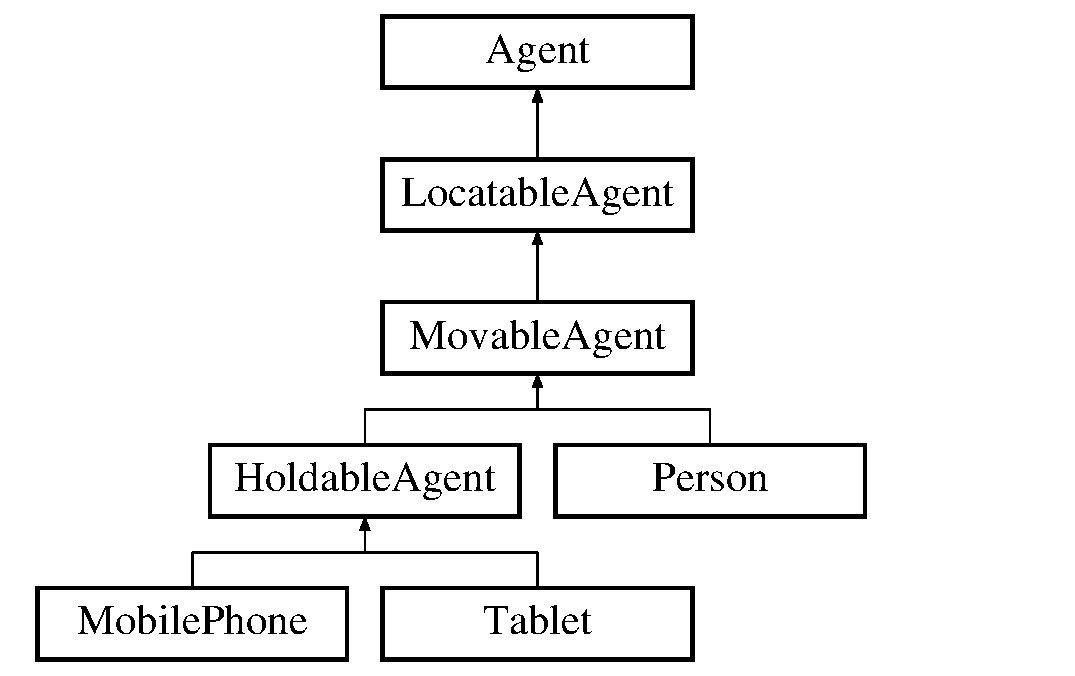
\includegraphics[height=5.000000cm]{class_movable_agent}
\end{center}
\end{figure}
\subsection*{Public Member Functions}
\begin{DoxyCompactItemize}
\item 
\textbf{ Movable\+Agent} (const \textbf{ Map} $\ast$m, const unsigned long id, Point $\ast$init\+Position, const \textbf{ Clock} $\ast$clock, double init\+Speed)
\item 
virtual \textbf{ $\sim$\+Movable\+Agent} ()
\item 
const string \textbf{ get\+Name} () const override
\item 
const string \textbf{ to\+String} () const override
\item 
virtual Point $\ast$ \textbf{ move} (\textbf{ Movement\+Type} type)=0
\item 
double \textbf{ get\+Speed} () const
\item 
void \textbf{ set\+Speed} (double speed)
\end{DoxyCompactItemize}
\subsection*{Private Attributes}
\begin{DoxyCompactItemize}
\item 
double \textbf{ m\+\_\+speed}
\end{DoxyCompactItemize}


\subsection{Detailed Description}
This class represents an agent that can move inside the map 

Definition at line 25 of file Movable\+Agent.\+h.



\subsection{Constructor \& Destructor Documentation}
\mbox{\label{class_movable_agent_ad76b14a044181a57ade71f1267a2ccbd}} 
\index{MovableAgent@{MovableAgent}!MovableAgent@{MovableAgent}}
\index{MovableAgent@{MovableAgent}!MovableAgent@{MovableAgent}}
\subsubsection{MovableAgent()}
{\footnotesize\ttfamily Movable\+Agent\+::\+Movable\+Agent (\begin{DoxyParamCaption}\item[{const \textbf{ Map} $\ast$}]{m,  }\item[{const unsigned long}]{id,  }\item[{Point $\ast$}]{init\+Position,  }\item[{const \textbf{ Clock} $\ast$}]{clock,  }\item[{double}]{init\+Speed }\end{DoxyParamCaption})\hspace{0.3cm}{\ttfamily [explicit]}}

Builds a new object with the parameters provided by user 
\begin{DoxyParams}{Parameters}
{\em m} & a pointer to the map used by the simulation \\
\hline
{\em id} & the id of the object \\
\hline
{\em init\+Position} & the initial location on map \\
\hline
{\em clock} & a pointer to the \doxyref{Clock}{p.}{class_clock} object used by this simulation \\
\hline
{\em init\+Speed} & the initial speed of the agent \\
\hline
\end{DoxyParams}
\mbox{\label{class_movable_agent_a20eb9ddcc953137e63e035837918206c}} 
\index{MovableAgent@{MovableAgent}!````~MovableAgent@{$\sim$MovableAgent}}
\index{````~MovableAgent@{$\sim$MovableAgent}!MovableAgent@{MovableAgent}}
\subsubsection{$\sim$MovableAgent()}
{\footnotesize\ttfamily virtual Movable\+Agent\+::$\sim$\+Movable\+Agent (\begin{DoxyParamCaption}{ }\end{DoxyParamCaption})\hspace{0.3cm}{\ttfamily [virtual]}}

Destructor 

\subsection{Member Function Documentation}
\mbox{\label{class_movable_agent_abcc1218876c39c996f2cb1eba2b96379}} 
\index{MovableAgent@{MovableAgent}!getName@{getName}}
\index{getName@{getName}!MovableAgent@{MovableAgent}}
\subsubsection{getName()}
{\footnotesize\ttfamily const string Movable\+Agent\+::get\+Name (\begin{DoxyParamCaption}{ }\end{DoxyParamCaption}) const\hspace{0.3cm}{\ttfamily [override]}, {\ttfamily [virtual]}}

Returns the name of the class \begin{DoxyReturn}{Returns}
the name of the class 
\end{DoxyReturn}


Reimplemented from \textbf{ Locatable\+Agent} \doxyref{}{p.}{class_locatable_agent_a754105958bb672744b525538f1584a7b}.



Reimplemented in \textbf{ Person} \doxyref{}{p.}{class_person_aa2a6f8d7f1d94045a03ca578f2ed272c}, and \textbf{ Tablet} \doxyref{}{p.}{class_tablet_adc7196aaee1e9714236b7cd8825d5826}.

\mbox{\label{class_movable_agent_a12fcdaee60f5bb29f15fe113a7dacaac}} 
\index{MovableAgent@{MovableAgent}!getSpeed@{getSpeed}}
\index{getSpeed@{getSpeed}!MovableAgent@{MovableAgent}}
\subsubsection{getSpeed()}
{\footnotesize\ttfamily double Movable\+Agent\+::get\+Speed (\begin{DoxyParamCaption}{ }\end{DoxyParamCaption}) const}

Returns the speed of this agent \begin{DoxyReturn}{Returns}
the speed of this agent 
\end{DoxyReturn}
\mbox{\label{class_movable_agent_a35299e133c6787689b553d74ce5f98f0}} 
\index{MovableAgent@{MovableAgent}!move@{move}}
\index{move@{move}!MovableAgent@{MovableAgent}}
\subsubsection{move()}
{\footnotesize\ttfamily virtual Point$\ast$ Movable\+Agent\+::move (\begin{DoxyParamCaption}\item[{\textbf{ Movement\+Type}}]{type }\end{DoxyParamCaption})\hspace{0.3cm}{\ttfamily [pure virtual]}}

A pure virtual method that moves the agent to a new location on the map 
\begin{DoxyParams}{Parameters}
{\em type} & the type of the movement. At this moment only \\
\hline
\end{DoxyParams}
\begin{DoxyReturn}{Returns}

\end{DoxyReturn}


Implemented in \textbf{ Person} \doxyref{}{p.}{class_person_a89843e85f14abc08422273c20252ae23}, \textbf{ Mobile\+Phone} \doxyref{}{p.}{class_mobile_phone_a92d77fa5810ddb9c4c482d9c9baea456}, and \textbf{ Tablet} \doxyref{}{p.}{class_tablet_a0021a8d61f496d84540f675b1cb7d080}.

\mbox{\label{class_movable_agent_ae2ef452e81789a4370e7dee32a9cc67e}} 
\index{MovableAgent@{MovableAgent}!setSpeed@{setSpeed}}
\index{setSpeed@{setSpeed}!MovableAgent@{MovableAgent}}
\subsubsection{setSpeed()}
{\footnotesize\ttfamily void Movable\+Agent\+::set\+Speed (\begin{DoxyParamCaption}\item[{double}]{speed }\end{DoxyParamCaption})}

Sets the speed of this agent 
\begin{DoxyParams}{Parameters}
{\em speed} & the speed of this agent \\
\hline
\end{DoxyParams}
\mbox{\label{class_movable_agent_a1dee2a6bf93f01006fadfb6fba6c9a59}} 
\index{MovableAgent@{MovableAgent}!toString@{toString}}
\index{toString@{toString}!MovableAgent@{MovableAgent}}
\subsubsection{toString()}
{\footnotesize\ttfamily const string Movable\+Agent\+::to\+String (\begin{DoxyParamCaption}{ }\end{DoxyParamCaption}) const\hspace{0.3cm}{\ttfamily [override]}, {\ttfamily [virtual]}}

Builds a human readable string representation of the agent \begin{DoxyReturn}{Returns}
a human readable string representation of the agent 
\end{DoxyReturn}


Reimplemented from \textbf{ Locatable\+Agent} \doxyref{}{p.}{class_locatable_agent_a88674f4c8ab9b1b2f3986b226bf4244f}.



Reimplemented in \textbf{ Person} \doxyref{}{p.}{class_person_a68872538da519d0a04297f43376db27c}, and \textbf{ Tablet} \doxyref{}{p.}{class_tablet_a3fae01e7d526699476221c6a686a4fba}.



\subsection{Member Data Documentation}
\mbox{\label{class_movable_agent_ac725b42e7b968740a59c3e1033d69ac5}} 
\index{MovableAgent@{MovableAgent}!m\_speed@{m\_speed}}
\index{m\_speed@{m\_speed}!MovableAgent@{MovableAgent}}
\subsubsection{m\_speed}
{\footnotesize\ttfamily double Movable\+Agent\+::m\+\_\+speed\hspace{0.3cm}{\ttfamily [private]}}



Definition at line 75 of file Movable\+Agent.\+h.



The documentation for this class was generated from the following file\+:\begin{DoxyCompactItemize}
\item 
include/\textbf{ Movable\+Agent.\+h}\end{DoxyCompactItemize}

\section{Parser Class Reference}
\label{class_parser}\index{Parser@{Parser}}


{\ttfamily \#include $<$C\+S\+Vparser.\+hpp$>$}

\subsection*{Public Member Functions}
\begin{DoxyCompactItemize}
\item 
\textbf{ Parser} (const string \&, const \textbf{ Data\+Type} \&type=\textbf{ e\+F\+I\+LE}, char sep=\textquotesingle{},\textquotesingle{}, bool has\+Header=true)
\item 
\textbf{ $\sim$\+Parser} (void)
\item 
\textbf{ Row} \& \textbf{ get\+Row} (unsigned int row) const
\item 
unsigned int \textbf{ row\+Count} (void) const
\item 
unsigned int \textbf{ column\+Count} (void) const
\item 
vector$<$ string $>$ \textbf{ get\+Header} (void) const
\item 
const string \textbf{ get\+Header\+Element} (unsigned int pos) const
\item 
const string \& \textbf{ get\+File\+Name} (void) const
\item 
bool \textbf{ delete\+Row} (unsigned int row)
\item 
bool \textbf{ add\+Row} (unsigned int pos, const vector$<$ string $>$ \&)
\item 
void \textbf{ sync} (void) const
\item 
\textbf{ Row} \& \textbf{ operator[$\,$]} (unsigned int row) const
\end{DoxyCompactItemize}
\subsection*{Protected Member Functions}
\begin{DoxyCompactItemize}
\item 
void \textbf{ parse\+Header} (void)
\item 
void \textbf{ parse\+Content} (void)
\end{DoxyCompactItemize}
\subsection*{Private Attributes}
\begin{DoxyCompactItemize}
\item 
string \textbf{ \+\_\+file}
\item 
const \textbf{ Data\+Type} \textbf{ \+\_\+type}
\item 
const char \textbf{ \+\_\+sep}
\item 
vector$<$ string $>$ \textbf{ \+\_\+original\+File}
\item 
vector$<$ string $>$ \textbf{ \+\_\+header}
\item 
vector$<$ \textbf{ Row} $\ast$ $>$ \textbf{ \+\_\+content}
\item 
bool \textbf{ m\+\_\+header}
\end{DoxyCompactItemize}


\subsection{Detailed Description}


Definition at line 57 of file C\+S\+Vparser.\+hpp.



\subsection{Constructor \& Destructor Documentation}
\mbox{\label{class_parser_acdb936b8a1723b1f342dfffbd6df310a}} 
\index{Parser@{Parser}!Parser@{Parser}}
\index{Parser@{Parser}!Parser@{Parser}}
\subsubsection{Parser()}
{\footnotesize\ttfamily Parser\+::\+Parser (\begin{DoxyParamCaption}\item[{const string \&}]{,  }\item[{const \textbf{ Data\+Type} \&}]{type = {\ttfamily \textbf{ e\+F\+I\+LE}},  }\item[{char}]{sep = {\ttfamily \textquotesingle{},\textquotesingle{}},  }\item[{bool}]{has\+Header = {\ttfamily true} }\end{DoxyParamCaption})}



Definition at line 9 of file C\+S\+V\+Parser.\+cpp.

\mbox{\label{class_parser_a1e70d9a903c5d2e8166fb571de3d581c}} 
\index{Parser@{Parser}!````~Parser@{$\sim$Parser}}
\index{````~Parser@{$\sim$Parser}!Parser@{Parser}}
\subsubsection{$\sim$Parser()}
{\footnotesize\ttfamily Parser\+::$\sim$\+Parser (\begin{DoxyParamCaption}\item[{void}]{ }\end{DoxyParamCaption})}



Definition at line 45 of file C\+S\+V\+Parser.\+cpp.



References \+\_\+content.



\subsection{Member Function Documentation}
\mbox{\label{class_parser_afe0f826abe9a149bbe798664cd9022ec}} 
\index{Parser@{Parser}!addRow@{addRow}}
\index{addRow@{addRow}!Parser@{Parser}}
\subsubsection{addRow()}
{\footnotesize\ttfamily bool Parser\+::add\+Row (\begin{DoxyParamCaption}\item[{unsigned int}]{pos,  }\item[{const vector$<$ string $>$ \&}]{r }\end{DoxyParamCaption})}



Definition at line 130 of file C\+S\+V\+Parser.\+cpp.



References \+\_\+content, \+\_\+header, and Row\+::push().

\mbox{\label{class_parser_a5f0dfff7f5168d2ca894319651f102e3}} 
\index{Parser@{Parser}!columnCount@{columnCount}}
\index{columnCount@{columnCount}!Parser@{Parser}}
\subsubsection{columnCount()}
{\footnotesize\ttfamily unsigned int Parser\+::column\+Count (\begin{DoxyParamCaption}\item[{void}]{ }\end{DoxyParamCaption}) const}



Definition at line 107 of file C\+S\+V\+Parser.\+cpp.



References \+\_\+header.

\mbox{\label{class_parser_a8f625a8081a5bde560d46d18d04efb2e}} 
\index{Parser@{Parser}!deleteRow@{deleteRow}}
\index{deleteRow@{deleteRow}!Parser@{Parser}}
\subsubsection{deleteRow()}
{\footnotesize\ttfamily bool Parser\+::delete\+Row (\begin{DoxyParamCaption}\item[{unsigned int}]{row }\end{DoxyParamCaption})}



Definition at line 121 of file C\+S\+V\+Parser.\+cpp.



References \+\_\+content.

\mbox{\label{class_parser_a3201b8253f4ea1c4420f3637c6c8de2b}} 
\index{Parser@{Parser}!getFileName@{getFileName}}
\index{getFileName@{getFileName}!Parser@{Parser}}
\subsubsection{getFileName()}
{\footnotesize\ttfamily const string \& Parser\+::get\+File\+Name (\begin{DoxyParamCaption}\item[{void}]{ }\end{DoxyParamCaption}) const}



Definition at line 165 of file C\+S\+V\+Parser.\+cpp.



References \+\_\+file.

\mbox{\label{class_parser_a0e9fb5d631e2e95685c67d8d59e1ba50}} 
\index{Parser@{Parser}!getHeader@{getHeader}}
\index{getHeader@{getHeader}!Parser@{Parser}}
\subsubsection{getHeader()}
{\footnotesize\ttfamily vector$<$ string $>$ Parser\+::get\+Header (\begin{DoxyParamCaption}\item[{void}]{ }\end{DoxyParamCaption}) const}



Definition at line 111 of file C\+S\+V\+Parser.\+cpp.



References \+\_\+header.

\mbox{\label{class_parser_adff671135239b5031b8eb937eb9cd844}} 
\index{Parser@{Parser}!getHeaderElement@{getHeaderElement}}
\index{getHeaderElement@{getHeaderElement}!Parser@{Parser}}
\subsubsection{getHeaderElement()}
{\footnotesize\ttfamily const string Parser\+::get\+Header\+Element (\begin{DoxyParamCaption}\item[{unsigned int}]{pos }\end{DoxyParamCaption}) const}



Definition at line 115 of file C\+S\+V\+Parser.\+cpp.



References \+\_\+header.

\mbox{\label{class_parser_a4cbc7632e6bb4841275884cbc128e25a}} 
\index{Parser@{Parser}!getRow@{getRow}}
\index{getRow@{getRow}!Parser@{Parser}}
\subsubsection{getRow()}
{\footnotesize\ttfamily \textbf{ Row} \& Parser\+::get\+Row (\begin{DoxyParamCaption}\item[{unsigned int}]{row }\end{DoxyParamCaption}) const}



Definition at line 93 of file C\+S\+V\+Parser.\+cpp.



References \+\_\+content.



Referenced by operator[$\,$]().

\mbox{\label{class_parser_a9c29df2f64942cac1dcc1f5d63b4fb36}} 
\index{Parser@{Parser}!operator[]@{operator[]}}
\index{operator[]@{operator[]}!Parser@{Parser}}
\subsubsection{operator[]()}
{\footnotesize\ttfamily \textbf{ Row} \& Parser\+::operator[$\,$] (\begin{DoxyParamCaption}\item[{unsigned int}]{row }\end{DoxyParamCaption}) const}



Definition at line 99 of file C\+S\+V\+Parser.\+cpp.



References get\+Row().

\mbox{\label{class_parser_a7fe27b82f7adf8633d633ee79e608012}} 
\index{Parser@{Parser}!parseContent@{parseContent}}
\index{parseContent@{parseContent}!Parser@{Parser}}
\subsubsection{parseContent()}
{\footnotesize\ttfamily void Parser\+::parse\+Content (\begin{DoxyParamCaption}\item[{void}]{ }\end{DoxyParamCaption})\hspace{0.3cm}{\ttfamily [protected]}}



Definition at line 60 of file C\+S\+V\+Parser.\+cpp.



References \+\_\+content, \+\_\+header, \+\_\+original\+File, m\+\_\+header, Row\+::push(), and Row\+::size().

\mbox{\label{class_parser_adf0f8593adc24b7c2c9318473afcf8e4}} 
\index{Parser@{Parser}!parseHeader@{parseHeader}}
\index{parseHeader@{parseHeader}!Parser@{Parser}}
\subsubsection{parseHeader()}
{\footnotesize\ttfamily void Parser\+::parse\+Header (\begin{DoxyParamCaption}\item[{void}]{ }\end{DoxyParamCaption})\hspace{0.3cm}{\ttfamily [protected]}}



Definition at line 52 of file C\+S\+V\+Parser.\+cpp.



References \+\_\+header, \+\_\+original\+File, and \+\_\+sep.

\mbox{\label{class_parser_a3cf277ff6ffc29b4be24adc8af113cc9}} 
\index{Parser@{Parser}!rowCount@{rowCount}}
\index{rowCount@{rowCount}!Parser@{Parser}}
\subsubsection{rowCount()}
{\footnotesize\ttfamily unsigned int Parser\+::row\+Count (\begin{DoxyParamCaption}\item[{void}]{ }\end{DoxyParamCaption}) const}



Definition at line 103 of file C\+S\+V\+Parser.\+cpp.



References \+\_\+content.

\mbox{\label{class_parser_aa92421ad7f5c4bb158b0b2f389458947}} 
\index{Parser@{Parser}!sync@{sync}}
\index{sync@{sync}!Parser@{Parser}}
\subsubsection{sync()}
{\footnotesize\ttfamily void Parser\+::sync (\begin{DoxyParamCaption}\item[{void}]{ }\end{DoxyParamCaption}) const}



Definition at line 143 of file C\+S\+V\+Parser.\+cpp.



References \+\_\+content, \+\_\+file, \+\_\+header, \+\_\+type, and e\+F\+I\+LE.



\subsection{Member Data Documentation}
\mbox{\label{class_parser_a47c9a793cb0869cb19a60883eebc469d}} 
\index{Parser@{Parser}!\_content@{\_content}}
\index{\_content@{\_content}!Parser@{Parser}}
\subsubsection{\_content}
{\footnotesize\ttfamily vector$<$\textbf{ Row} $\ast$$>$ Parser\+::\+\_\+content\hspace{0.3cm}{\ttfamily [private]}}



Definition at line 86 of file C\+S\+Vparser.\+hpp.



Referenced by add\+Row(), delete\+Row(), get\+Row(), parse\+Content(), row\+Count(), sync(), and $\sim$\+Parser().

\mbox{\label{class_parser_af173d4c3df007ee81d42887b4a15060a}} 
\index{Parser@{Parser}!\_file@{\_file}}
\index{\_file@{\_file}!Parser@{Parser}}
\subsubsection{\_file}
{\footnotesize\ttfamily string Parser\+::\+\_\+file\hspace{0.3cm}{\ttfamily [private]}}



Definition at line 81 of file C\+S\+Vparser.\+hpp.



Referenced by get\+File\+Name(), and sync().

\mbox{\label{class_parser_aa4b3a567bac767923745b4bd2f176c6f}} 
\index{Parser@{Parser}!\_header@{\_header}}
\index{\_header@{\_header}!Parser@{Parser}}
\subsubsection{\_header}
{\footnotesize\ttfamily vector$<$string$>$ Parser\+::\+\_\+header\hspace{0.3cm}{\ttfamily [private]}}



Definition at line 85 of file C\+S\+Vparser.\+hpp.



Referenced by add\+Row(), column\+Count(), get\+Header(), get\+Header\+Element(), parse\+Content(), parse\+Header(), and sync().

\mbox{\label{class_parser_abecadd4e857d14479da2fa7ec344f21b}} 
\index{Parser@{Parser}!\_originalFile@{\_originalFile}}
\index{\_originalFile@{\_originalFile}!Parser@{Parser}}
\subsubsection{\_originalFile}
{\footnotesize\ttfamily vector$<$string$>$ Parser\+::\+\_\+original\+File\hspace{0.3cm}{\ttfamily [private]}}



Definition at line 84 of file C\+S\+Vparser.\+hpp.



Referenced by parse\+Content(), and parse\+Header().

\mbox{\label{class_parser_ae09c229a5f86b536e11fe4f1a3274317}} 
\index{Parser@{Parser}!\_sep@{\_sep}}
\index{\_sep@{\_sep}!Parser@{Parser}}
\subsubsection{\_sep}
{\footnotesize\ttfamily const char Parser\+::\+\_\+sep\hspace{0.3cm}{\ttfamily [private]}}



Definition at line 83 of file C\+S\+Vparser.\+hpp.



Referenced by parse\+Header().

\mbox{\label{class_parser_a40e8d80f6539cd6170a25d47b9edb20c}} 
\index{Parser@{Parser}!\_type@{\_type}}
\index{\_type@{\_type}!Parser@{Parser}}
\subsubsection{\_type}
{\footnotesize\ttfamily const \textbf{ Data\+Type} Parser\+::\+\_\+type\hspace{0.3cm}{\ttfamily [private]}}



Definition at line 82 of file C\+S\+Vparser.\+hpp.



Referenced by sync().

\mbox{\label{class_parser_ab0bd343f86055468eb6cbd298dacdc16}} 
\index{Parser@{Parser}!m\_header@{m\_header}}
\index{m\_header@{m\_header}!Parser@{Parser}}
\subsubsection{m\_header}
{\footnotesize\ttfamily bool Parser\+::m\+\_\+header\hspace{0.3cm}{\ttfamily [private]}}



Definition at line 87 of file C\+S\+Vparser.\+hpp.



Referenced by parse\+Content().



The documentation for this class was generated from the following files\+:\begin{DoxyCompactItemize}
\item 
include/\textbf{ C\+S\+Vparser.\+hpp}\item 
src/\textbf{ C\+S\+V\+Parser.\+cpp}\end{DoxyCompactItemize}

\hypertarget{class_person}{}\section{Person Class Reference}
\label{class_person}\index{Person@{Person}}


{\ttfamily \#include $<$Person.\+h$>$}



Inheritance diagram for Person\+:
\nopagebreak
\begin{figure}[H]
\begin{center}
\leavevmode
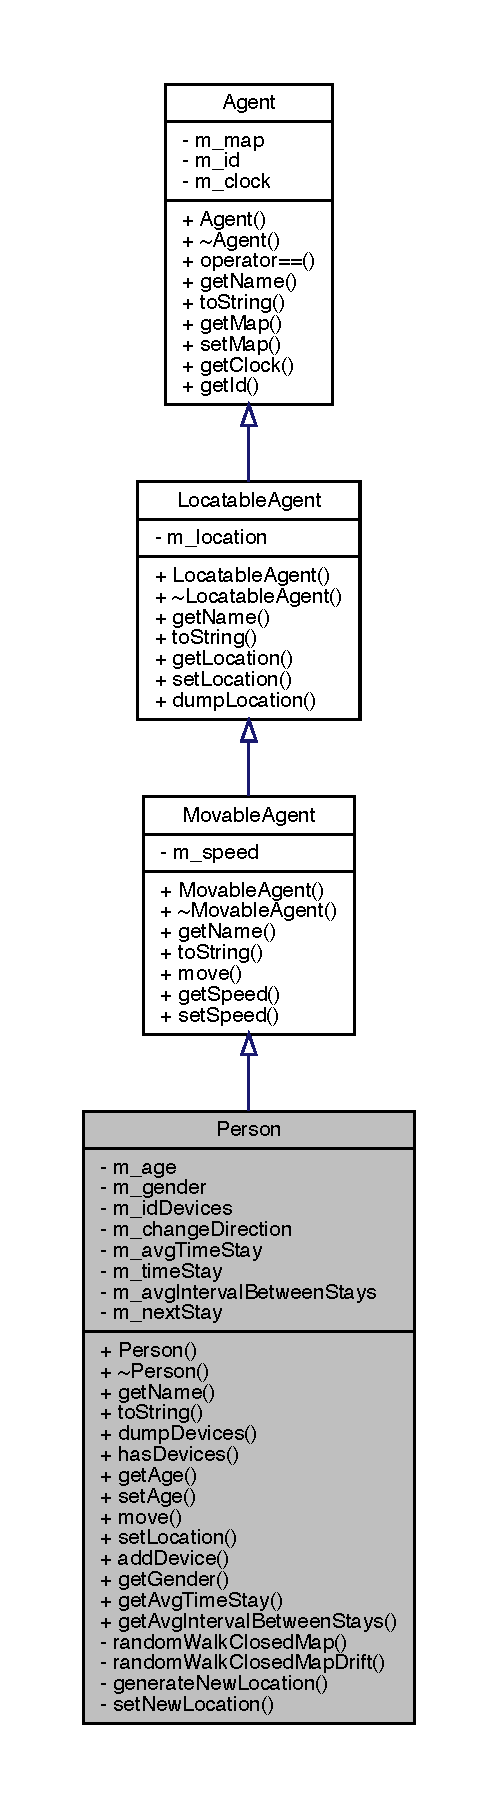
\includegraphics[height=550pt]{class_person__inherit__graph}
\end{center}
\end{figure}


Collaboration diagram for Person\+:
\nopagebreak
\begin{figure}[H]
\begin{center}
\leavevmode
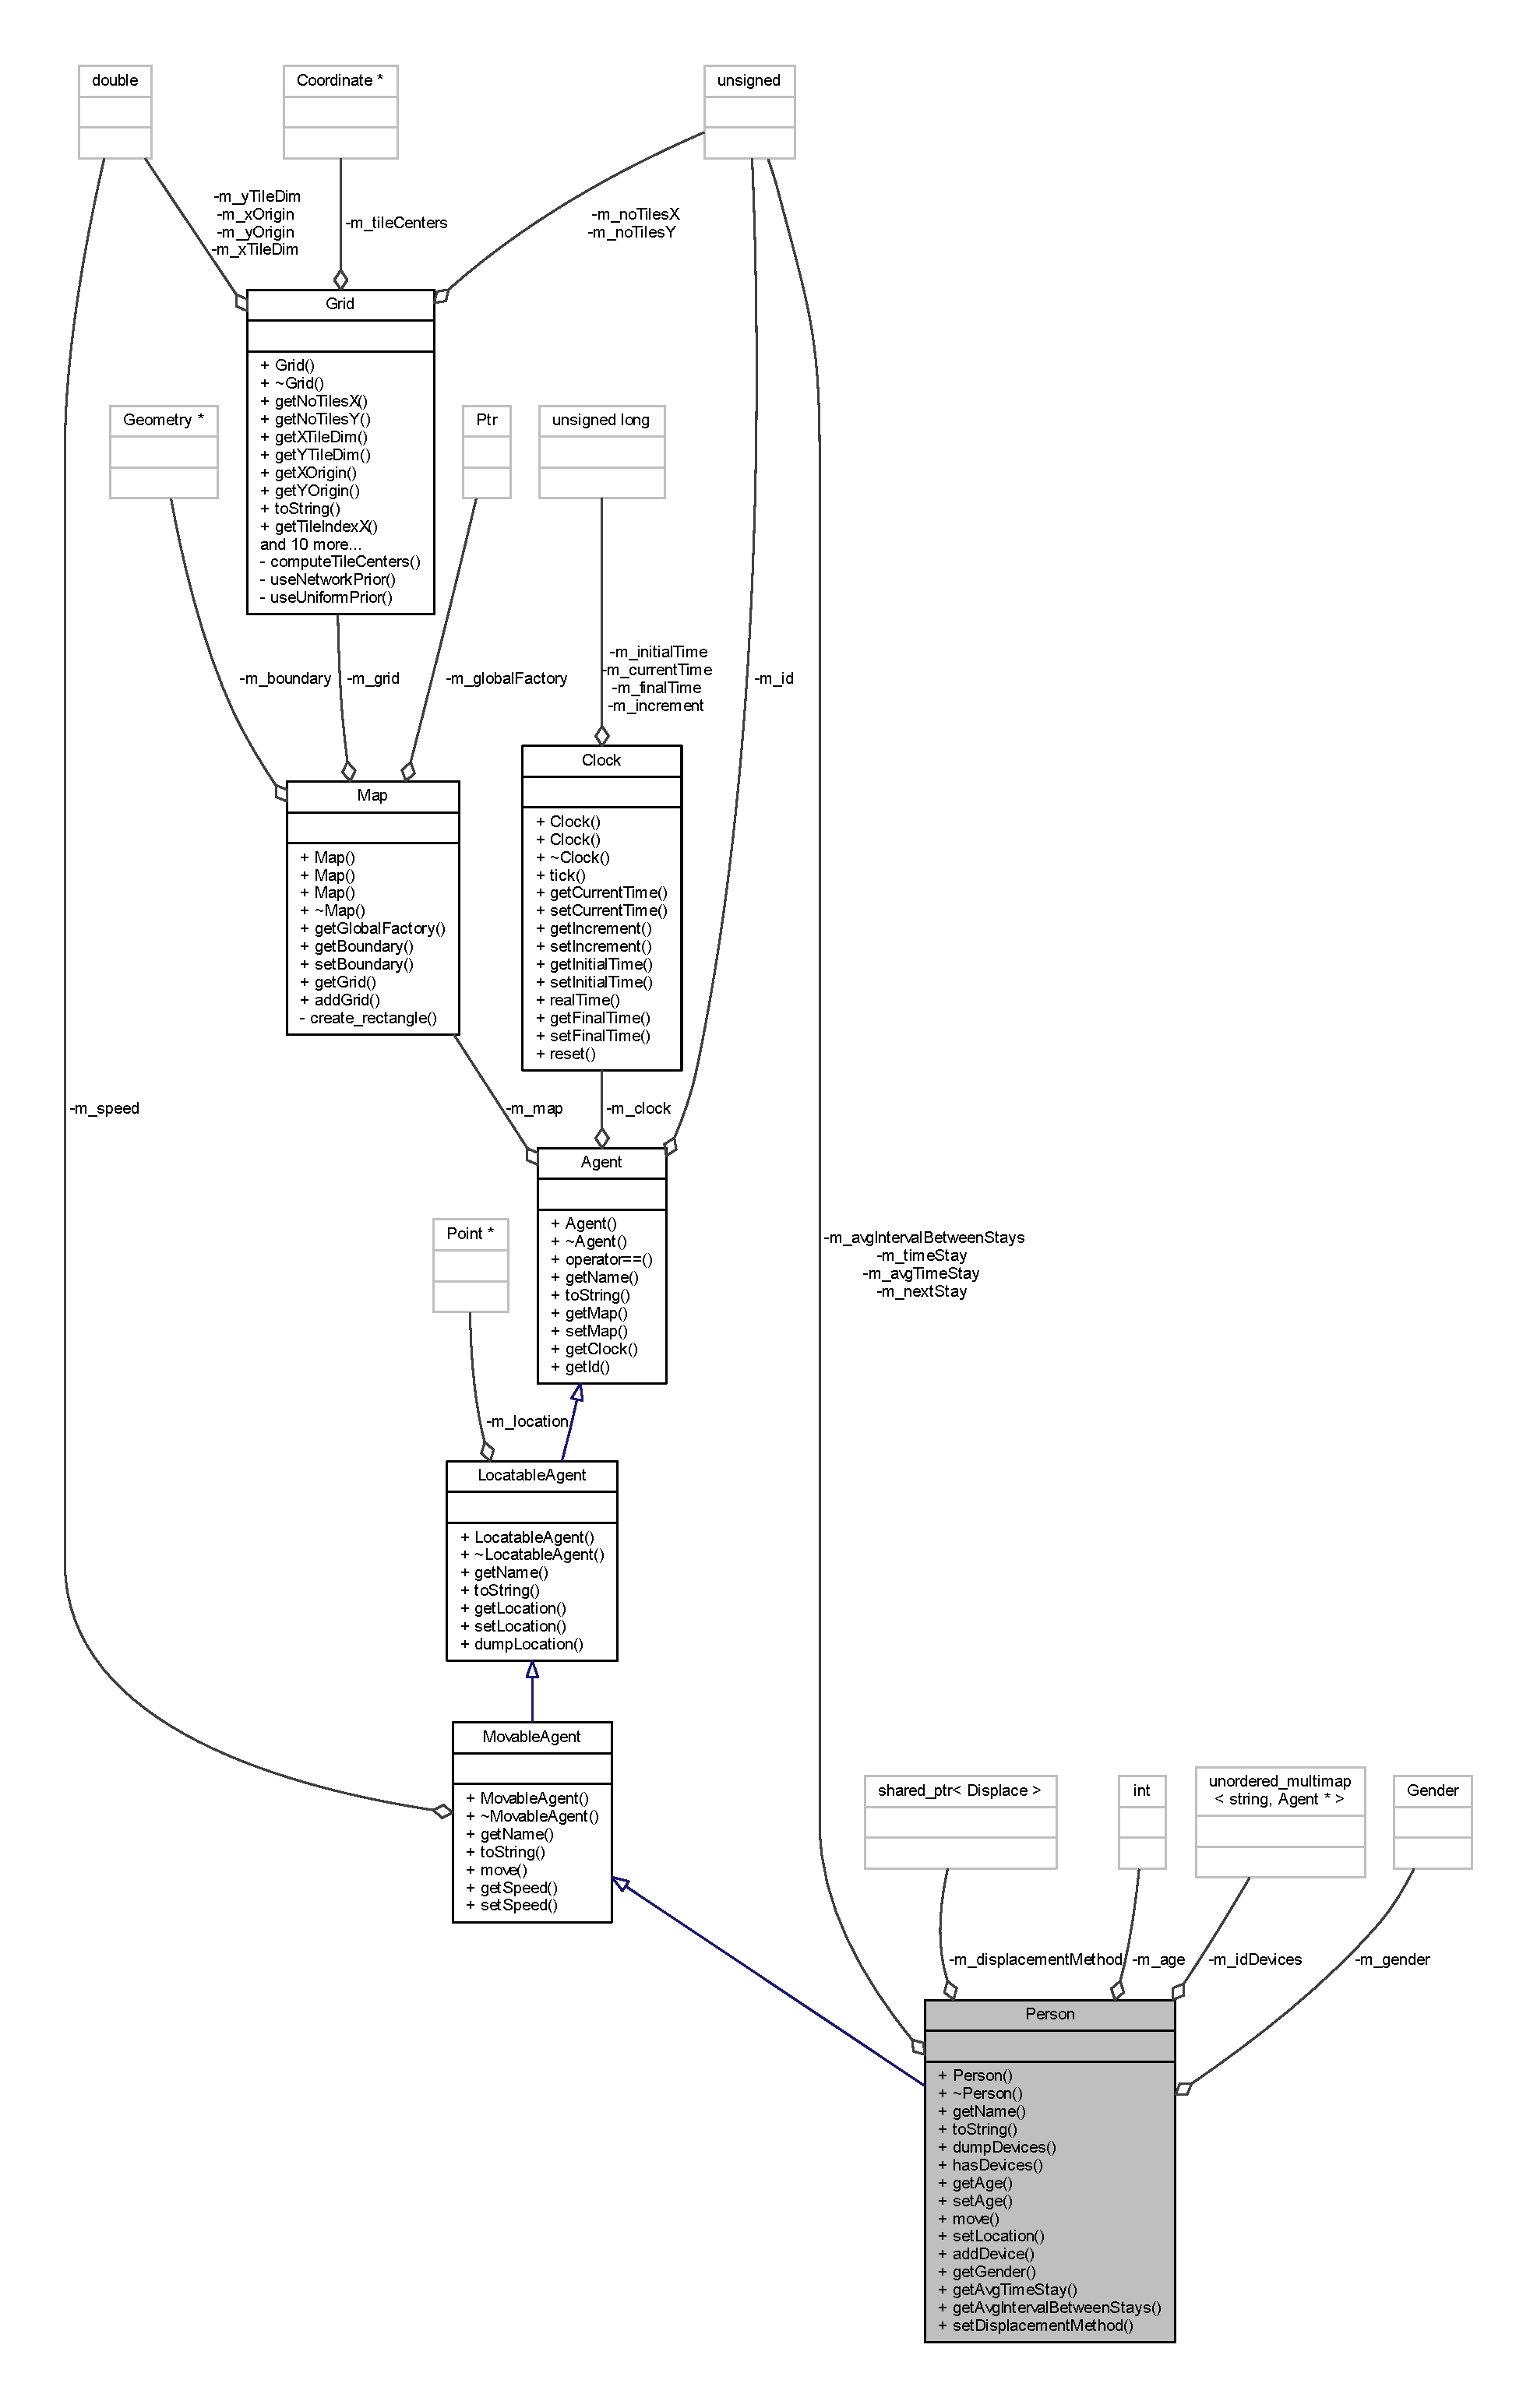
\includegraphics[height=550pt]{class_person__coll__graph}
\end{center}
\end{figure}
\subsection*{Public Types}
\begin{DoxyCompactItemize}
\item 
enum \hyperlink{class_person_aff84ca16bd4dbf364614d86f20b29dd2}{Gender} \{ \hyperlink{class_person_aff84ca16bd4dbf364614d86f20b29dd2a16691f7cc6595f87b71d9b43ad23fcb4}{M\+A\+LE}, 
\hyperlink{class_person_aff84ca16bd4dbf364614d86f20b29dd2a8ee21010fb2d8e8794ef72be368da064}{F\+E\+M\+A\+LE}
 \}
\end{DoxyCompactItemize}
\subsection*{Public Member Functions}
\begin{DoxyCompactItemize}
\item 
\hyperlink{class_person_a1fb64d7ef7c528d01dd09b2099b00e38}{Person} (const \hyperlink{class_map}{Map} $\ast$m, const unsigned long id, Point $\ast$init\+Position, const \hyperlink{class_clock}{Clock} $\ast$clock, double init\+Speed, int age, \hyperlink{class_person_aff84ca16bd4dbf364614d86f20b29dd2}{Gender} gender, unsigned long time\+Stay, unsigned long interval\+Between\+Stays)
\item 
virtual \hyperlink{class_person_a6b5729bb56531c93312b1179c8ee4b71}{$\sim$\+Person} ()
\item 
const string \hyperlink{class_person_a68872538da519d0a04297f43376db27c}{to\+String} () const override
\item 
string \hyperlink{class_person_a0bc06f77b3e8a151f8c5cc77459895c9}{dump\+Devices} ()
\item 
bool \hyperlink{class_person_a40d6f2c716dd3c9794067817a3fb9165}{has\+Devices} ()
\item 
int \hyperlink{class_person_a4b66dbee570398920b8fb6aacddd2559}{get\+Age} () const
\item 
void \hyperlink{class_person_ac8ade54c27a0657c987c395ff04a9d46}{set\+Age} (int age)
\item 
virtual Point $\ast$ \hyperlink{class_person_a922e0462a1e7eac6523a9a864ce27afc}{move} () override
\item 
virtual void \hyperlink{class_person_a05f4ac2107d59e03f0f336eda08aa358}{set\+Location} (Point $\ast$pt) override
\item 
void \hyperlink{class_person_a3ce0a72a98c2e723e48dcd7b4d9af599}{add\+Device} (string type, \hyperlink{class_agent}{Agent} $\ast$agent)
\item 
void \hyperlink{class_person_a89ada26d3541bc82e514dae833dc959d}{set\+Displacement\+Method} (const shared\+\_\+ptr$<$ \hyperlink{class_displace}{Displace} $>$ \&displace)
\end{DoxyCompactItemize}
\subsection*{Static Public Member Functions}
\begin{DoxyCompactItemize}
\item 
static const string \hyperlink{class_person_a6bebe59c354f26f4cb983185d6084181}{get\+Header} ()
\end{DoxyCompactItemize}
\subsection*{Private Attributes}
\begin{DoxyCompactItemize}
\item 
int \hyperlink{class_person_a743e071da10a5ac9150f61df919cfbb4}{m\+\_\+age}
\item 
\hyperlink{class_person_aff84ca16bd4dbf364614d86f20b29dd2}{Gender} \hyperlink{class_person_ade9cdf49acde95c75f19f0b0d24c8c9a}{m\+\_\+gender}
\item 
unordered\+\_\+multimap$<$ string, \hyperlink{class_agent}{Agent} $\ast$ $>$ \hyperlink{class_person_a95b2e60a54b72aea51a7600048e76291}{m\+\_\+id\+Devices}
\item 
unsigned long \hyperlink{class_person_a8c9502459dd59182d11f60f429b44457}{m\+\_\+avg\+Time\+Stay}
\item 
unsigned long \hyperlink{class_person_a5554109f1f3a7c466f02346d0061c6e7}{m\+\_\+time\+Stay}
\item 
unsigned long \hyperlink{class_person_a62a07c9565931a618a09be7510dde07c}{m\+\_\+avg\+Interval\+Between\+Stays}
\item 
unsigned long \hyperlink{class_person_ad8809184fc32b28b1bcc115b10493b55}{m\+\_\+next\+Stay}
\item 
shared\+\_\+ptr$<$ \hyperlink{class_displace}{Displace} $>$ \hyperlink{class_person_a92ceead10a7ca858d2151391e4421843}{m\+\_\+displacement\+Method}
\end{DoxyCompactItemize}


\subsection{Detailed Description}
This class represents a person that can have 0,1 or 2 mobile phone(s). During the simulation the person move around the map, carrying his/her mobile devices. 

\subsection{Member Enumeration Documentation}
\mbox{\Hypertarget{class_person_aff84ca16bd4dbf364614d86f20b29dd2}\label{class_person_aff84ca16bd4dbf364614d86f20b29dd2}} 
\index{Person@{Person}!Gender@{Gender}}
\index{Gender@{Gender}!Person@{Person}}
\subsubsection{\texorpdfstring{Gender}{Gender}}
{\footnotesize\ttfamily enum \hyperlink{class_person_aff84ca16bd4dbf364614d86f20b29dd2}{Person\+::\+Gender}}

\begin{DoxyEnumFields}{Enumerator}
\raisebox{\heightof{T}}[0pt][0pt]{\index{M\+A\+LE@{M\+A\+LE}!Person@{Person}}\index{Person@{Person}!M\+A\+LE@{M\+A\+LE}}}\mbox{\Hypertarget{class_person_aff84ca16bd4dbf364614d86f20b29dd2a16691f7cc6595f87b71d9b43ad23fcb4}\label{class_person_aff84ca16bd4dbf364614d86f20b29dd2a16691f7cc6595f87b71d9b43ad23fcb4}} 
M\+A\+LE&\\
\hline

\raisebox{\heightof{T}}[0pt][0pt]{\index{F\+E\+M\+A\+LE@{F\+E\+M\+A\+LE}!Person@{Person}}\index{Person@{Person}!F\+E\+M\+A\+LE@{F\+E\+M\+A\+LE}}}\mbox{\Hypertarget{class_person_aff84ca16bd4dbf364614d86f20b29dd2a8ee21010fb2d8e8794ef72be368da064}\label{class_person_aff84ca16bd4dbf364614d86f20b29dd2a8ee21010fb2d8e8794ef72be368da064}} 
F\+E\+M\+A\+LE&\\
\hline

\end{DoxyEnumFields}


\subsection{Constructor \& Destructor Documentation}
\mbox{\Hypertarget{class_person_a1fb64d7ef7c528d01dd09b2099b00e38}\label{class_person_a1fb64d7ef7c528d01dd09b2099b00e38}} 
\index{Person@{Person}!Person@{Person}}
\index{Person@{Person}!Person@{Person}}
\subsubsection{\texorpdfstring{Person()}{Person()}}
{\footnotesize\ttfamily Person\+::\+Person (\begin{DoxyParamCaption}\item[{const \hyperlink{class_map}{Map} $\ast$}]{m,  }\item[{const unsigned long}]{id,  }\item[{Point $\ast$}]{init\+Position,  }\item[{const \hyperlink{class_clock}{Clock} $\ast$}]{clock,  }\item[{double}]{init\+Speed,  }\item[{int}]{age,  }\item[{\hyperlink{class_person_aff84ca16bd4dbf364614d86f20b29dd2}{Gender}}]{gender,  }\item[{unsigned long}]{time\+Stay,  }\item[{unsigned long}]{interval\+Between\+Stays }\end{DoxyParamCaption})\hspace{0.3cm}{\ttfamily [explicit]}}

Builds a new \hyperlink{class_person}{Person} object with the characteristics given as parameters. 
\begin{DoxyParams}{Parameters}
{\em m} & a pointer to the \hyperlink{class_map}{Map} object where this \hyperlink{class_person}{Person} move. \\
\hline
{\em id} & the id of the \hyperlink{class_person}{Person}. \\
\hline
{\em init\+Position} & the initial location of the person on the map. \\
\hline
{\em clock} & a pointer to a \hyperlink{class_clock}{Clock} object used for this simulation. \\
\hline
{\em init\+Speed} & the initial speed of this person. It is provided in the configuration file. \\
\hline
{\em age} & the age of the person. The age is generated using a uniform or a normal distribution. \\
\hline
{\em gender} & the gender of the person. \\
\hline
{\em time\+Stay} & the average time of a stop \\
\hline
{\em interval\+Between\+Stays} & the average time between two consecutive stops. \\
\hline
\end{DoxyParams}
\mbox{\Hypertarget{class_person_a6b5729bb56531c93312b1179c8ee4b71}\label{class_person_a6b5729bb56531c93312b1179c8ee4b71}} 
\index{Person@{Person}!````~Person@{$\sim$\+Person}}
\index{````~Person@{$\sim$\+Person}!Person@{Person}}
\subsubsection{\texorpdfstring{$\sim$\+Person()}{~Person()}}
{\footnotesize\ttfamily virtual Person\+::$\sim$\+Person (\begin{DoxyParamCaption}{ }\end{DoxyParamCaption})\hspace{0.3cm}{\ttfamily [virtual]}}

The default destructor. 

\subsection{Member Function Documentation}
\mbox{\Hypertarget{class_person_a3ce0a72a98c2e723e48dcd7b4d9af599}\label{class_person_a3ce0a72a98c2e723e48dcd7b4d9af599}} 
\index{Person@{Person}!add\+Device@{add\+Device}}
\index{add\+Device@{add\+Device}!Person@{Person}}
\subsubsection{\texorpdfstring{add\+Device()}{addDevice()}}
{\footnotesize\ttfamily void Person\+::add\+Device (\begin{DoxyParamCaption}\item[{string}]{type,  }\item[{\hyperlink{class_agent}{Agent} $\ast$}]{agent }\end{DoxyParamCaption})}

Add a mobile device to this person. Internally, all mobile devices are kept in an unordered\+\_\+multimap as pairs $<$name of the device class, pointer to the device object$>$ 
\begin{DoxyParams}{Parameters}
{\em type} & the name of the device\textquotesingle{}s class. \\
\hline
{\em agent} & a pointer to the device object. \\
\hline
\end{DoxyParams}
\mbox{\Hypertarget{class_person_a0bc06f77b3e8a151f8c5cc77459895c9}\label{class_person_a0bc06f77b3e8a151f8c5cc77459895c9}} 
\index{Person@{Person}!dump\+Devices@{dump\+Devices}}
\index{dump\+Devices@{dump\+Devices}!Person@{Person}}
\subsubsection{\texorpdfstring{dump\+Devices()}{dumpDevices()}}
{\footnotesize\ttfamily string Person\+::dump\+Devices (\begin{DoxyParamCaption}{ }\end{DoxyParamCaption})}

Builds a string containing a list with the ids of the mobile devices that this person owns. \begin{DoxyReturn}{Returns}
a string containing a list with the ids of the mobile devices that this person owns. 
\end{DoxyReturn}
\mbox{\Hypertarget{class_person_a4b66dbee570398920b8fb6aacddd2559}\label{class_person_a4b66dbee570398920b8fb6aacddd2559}} 
\index{Person@{Person}!get\+Age@{get\+Age}}
\index{get\+Age@{get\+Age}!Person@{Person}}
\subsubsection{\texorpdfstring{get\+Age()}{getAge()}}
{\footnotesize\ttfamily int Person\+::get\+Age (\begin{DoxyParamCaption}{ }\end{DoxyParamCaption}) const}

Returns the age of the person. \begin{DoxyReturn}{Returns}
the age of the person. 
\end{DoxyReturn}
\mbox{\Hypertarget{class_person_a6bebe59c354f26f4cb983185d6084181}\label{class_person_a6bebe59c354f26f4cb983185d6084181}} 
\index{Person@{Person}!get\+Header@{get\+Header}}
\index{get\+Header@{get\+Header}!Person@{Person}}
\subsubsection{\texorpdfstring{get\+Header()}{getHeader()}}
{\footnotesize\ttfamily static const string Person\+::get\+Header (\begin{DoxyParamCaption}{ }\end{DoxyParamCaption})\hspace{0.3cm}{\ttfamily [static]}}

\mbox{\Hypertarget{class_person_a40d6f2c716dd3c9794067817a3fb9165}\label{class_person_a40d6f2c716dd3c9794067817a3fb9165}} 
\index{Person@{Person}!has\+Devices@{has\+Devices}}
\index{has\+Devices@{has\+Devices}!Person@{Person}}
\subsubsection{\texorpdfstring{has\+Devices()}{hasDevices()}}
{\footnotesize\ttfamily bool Person\+::has\+Devices (\begin{DoxyParamCaption}{ }\end{DoxyParamCaption})}

returns true if this person has at least a mobile device, false otherwise. \begin{DoxyReturn}{Returns}

\end{DoxyReturn}
\mbox{\Hypertarget{class_person_a922e0462a1e7eac6523a9a864ce27afc}\label{class_person_a922e0462a1e7eac6523a9a864ce27afc}} 
\index{Person@{Person}!move@{move}}
\index{move@{move}!Person@{Person}}
\subsubsection{\texorpdfstring{move()}{move()}}
{\footnotesize\ttfamily virtual Point$\ast$ Person\+::move (\begin{DoxyParamCaption}{ }\end{DoxyParamCaption})\hspace{0.3cm}{\ttfamily [override]}, {\ttfamily [virtual]}}

Makes a step on the map according to an algorithm. The direction and the length of the step is determined by the displacement strategy set at the \hyperlink{class_person}{Person} creation moment and currently two strategies are supported\+: \hyperlink{class_random_walk_displacement}{Random\+Walk\+Displacement} and \hyperlink{class_random_walk_drift_displacement}{Random\+Walk\+Drift\+Displacement}. \hyperlink{class_random_walk_displacement}{Random\+Walk\+Displacement} means that at each time instant the direction is generated as a uniformly distributed random value and the step length is computed multiplying the speed with the time interval set in the simulation configuration file. If a step projects it outside the map, it stops on the boundary. \hyperlink{class_random_walk_drift_displacement}{Random\+Walk\+Drift\+Displacement} means that there is a preference in the direction of the movement. There are two constants defined, S\+I\+M\+\_\+\+T\+R\+E\+N\+D\+\_\+\+A\+N\+G\+L\+E\+\_\+1 and S\+I\+M\+\_\+\+T\+R\+E\+N\+D\+\_\+\+A\+N\+G\+L\+E\+\_\+2 (3\+P\+I/4 and 5\+P\+I/4), and in the first half of the simulation the direction is generated as a normal distributed random value with the mean equals to S\+I\+M\+\_\+\+T\+R\+E\+N\+D\+\_\+\+A\+N\+G\+L\+E\+\_\+1 and sd = 0.\+1 while during the second half of the simulation it is generated as a normal distributed random value with the mean equals to S\+I\+M\+\_\+\+T\+R\+E\+N\+D\+\_\+\+A\+N\+G\+L\+E\+\_\+2 and the same sd. Again, any kind of \hyperlink{class_movable_agent}{Movable\+Agent} can only move inside the map boundary. If a step projects it outside the map, it stops on the boundary. \begin{DoxyReturn}{Returns}
the final location after the displacement. 
\end{DoxyReturn}


Implements \hyperlink{class_movable_agent_a88b617f0e78c817634e5b587da045ab0}{Movable\+Agent}.

\mbox{\Hypertarget{class_person_ac8ade54c27a0657c987c395ff04a9d46}\label{class_person_ac8ade54c27a0657c987c395ff04a9d46}} 
\index{Person@{Person}!set\+Age@{set\+Age}}
\index{set\+Age@{set\+Age}!Person@{Person}}
\subsubsection{\texorpdfstring{set\+Age()}{setAge()}}
{\footnotesize\ttfamily void Person\+::set\+Age (\begin{DoxyParamCaption}\item[{int}]{age }\end{DoxyParamCaption})}

Sets the age of the person. 
\begin{DoxyParams}{Parameters}
{\em age} & the age of the person. \\
\hline
\end{DoxyParams}
\mbox{\Hypertarget{class_person_a89ada26d3541bc82e514dae833dc959d}\label{class_person_a89ada26d3541bc82e514dae833dc959d}} 
\index{Person@{Person}!set\+Displacement\+Method@{set\+Displacement\+Method}}
\index{set\+Displacement\+Method@{set\+Displacement\+Method}!Person@{Person}}
\subsubsection{\texorpdfstring{set\+Displacement\+Method()}{setDisplacementMethod()}}
{\footnotesize\ttfamily void Person\+::set\+Displacement\+Method (\begin{DoxyParamCaption}\item[{const shared\+\_\+ptr$<$ \hyperlink{class_displace}{Displace} $>$ \&}]{displace }\end{DoxyParamCaption})}

Sets the displacement algorithm. 
\begin{DoxyParams}{Parameters}
{\em displace} & a reference to an implementation of the displacement method. Currently two displacement methods are supported and they are implemented in \hyperlink{class_random_walk_displacement}{Random\+Walk\+Displacement} and \hyperlink{class_random_walk_drift_displacement}{Random\+Walk\+Drift\+Displacement} classes. \\
\hline
\end{DoxyParams}
\mbox{\Hypertarget{class_person_a05f4ac2107d59e03f0f336eda08aa358}\label{class_person_a05f4ac2107d59e03f0f336eda08aa358}} 
\index{Person@{Person}!set\+Location@{set\+Location}}
\index{set\+Location@{set\+Location}!Person@{Person}}
\subsubsection{\texorpdfstring{set\+Location()}{setLocation()}}
{\footnotesize\ttfamily virtual void Person\+::set\+Location (\begin{DoxyParamCaption}\item[{Point $\ast$}]{pt }\end{DoxyParamCaption})\hspace{0.3cm}{\ttfamily [override]}, {\ttfamily [virtual]}}

Sets the location of the person on the map. 
\begin{DoxyParams}{Parameters}
{\em pt} & a pointer to a Point object that represent the location of the person on the map. If the person has mobile devices (phone, tablets) this function calls \hyperlink{class_person_a05f4ac2107d59e03f0f336eda08aa358}{set\+Location()} for all mobile devices too. \\
\hline
\end{DoxyParams}


Reimplemented from \hyperlink{class_locatable_agent_a754b237c404b77714fedd397f214bc02}{Locatable\+Agent}.

\mbox{\Hypertarget{class_person_a68872538da519d0a04297f43376db27c}\label{class_person_a68872538da519d0a04297f43376db27c}} 
\index{Person@{Person}!to\+String@{to\+String}}
\index{to\+String@{to\+String}!Person@{Person}}
\subsubsection{\texorpdfstring{to\+String()}{toString()}}
{\footnotesize\ttfamily const string Person\+::to\+String (\begin{DoxyParamCaption}{ }\end{DoxyParamCaption}) const\hspace{0.3cm}{\ttfamily [override]}, {\ttfamily [virtual]}}

Builds and returns a human readable string representation of the person. \begin{DoxyReturn}{Returns}
a human readable string representation of the person. 
\end{DoxyReturn}


Reimplemented from \hyperlink{class_movable_agent_a1dee2a6bf93f01006fadfb6fba6c9a59}{Movable\+Agent}.



\subsection{Member Data Documentation}
\mbox{\Hypertarget{class_person_a743e071da10a5ac9150f61df919cfbb4}\label{class_person_a743e071da10a5ac9150f61df919cfbb4}} 
\index{Person@{Person}!m\+\_\+age@{m\+\_\+age}}
\index{m\+\_\+age@{m\+\_\+age}!Person@{Person}}
\subsubsection{\texorpdfstring{m\+\_\+age}{m\_age}}
{\footnotesize\ttfamily int Person\+::m\+\_\+age\hspace{0.3cm}{\ttfamily [private]}}

\mbox{\Hypertarget{class_person_a62a07c9565931a618a09be7510dde07c}\label{class_person_a62a07c9565931a618a09be7510dde07c}} 
\index{Person@{Person}!m\+\_\+avg\+Interval\+Between\+Stays@{m\+\_\+avg\+Interval\+Between\+Stays}}
\index{m\+\_\+avg\+Interval\+Between\+Stays@{m\+\_\+avg\+Interval\+Between\+Stays}!Person@{Person}}
\subsubsection{\texorpdfstring{m\+\_\+avg\+Interval\+Between\+Stays}{m\_avgIntervalBetweenStays}}
{\footnotesize\ttfamily unsigned long Person\+::m\+\_\+avg\+Interval\+Between\+Stays\hspace{0.3cm}{\ttfamily [private]}}

\mbox{\Hypertarget{class_person_a8c9502459dd59182d11f60f429b44457}\label{class_person_a8c9502459dd59182d11f60f429b44457}} 
\index{Person@{Person}!m\+\_\+avg\+Time\+Stay@{m\+\_\+avg\+Time\+Stay}}
\index{m\+\_\+avg\+Time\+Stay@{m\+\_\+avg\+Time\+Stay}!Person@{Person}}
\subsubsection{\texorpdfstring{m\+\_\+avg\+Time\+Stay}{m\_avgTimeStay}}
{\footnotesize\ttfamily unsigned long Person\+::m\+\_\+avg\+Time\+Stay\hspace{0.3cm}{\ttfamily [private]}}

\mbox{\Hypertarget{class_person_a92ceead10a7ca858d2151391e4421843}\label{class_person_a92ceead10a7ca858d2151391e4421843}} 
\index{Person@{Person}!m\+\_\+displacement\+Method@{m\+\_\+displacement\+Method}}
\index{m\+\_\+displacement\+Method@{m\+\_\+displacement\+Method}!Person@{Person}}
\subsubsection{\texorpdfstring{m\+\_\+displacement\+Method}{m\_displacementMethod}}
{\footnotesize\ttfamily shared\+\_\+ptr$<$\hyperlink{class_displace}{Displace}$>$ Person\+::m\+\_\+displacement\+Method\hspace{0.3cm}{\ttfamily [private]}}

\mbox{\Hypertarget{class_person_ade9cdf49acde95c75f19f0b0d24c8c9a}\label{class_person_ade9cdf49acde95c75f19f0b0d24c8c9a}} 
\index{Person@{Person}!m\+\_\+gender@{m\+\_\+gender}}
\index{m\+\_\+gender@{m\+\_\+gender}!Person@{Person}}
\subsubsection{\texorpdfstring{m\+\_\+gender}{m\_gender}}
{\footnotesize\ttfamily \hyperlink{class_person_aff84ca16bd4dbf364614d86f20b29dd2}{Gender} Person\+::m\+\_\+gender\hspace{0.3cm}{\ttfamily [private]}}

\mbox{\Hypertarget{class_person_a95b2e60a54b72aea51a7600048e76291}\label{class_person_a95b2e60a54b72aea51a7600048e76291}} 
\index{Person@{Person}!m\+\_\+id\+Devices@{m\+\_\+id\+Devices}}
\index{m\+\_\+id\+Devices@{m\+\_\+id\+Devices}!Person@{Person}}
\subsubsection{\texorpdfstring{m\+\_\+id\+Devices}{m\_idDevices}}
{\footnotesize\ttfamily unordered\+\_\+multimap$<$string, \hyperlink{class_agent}{Agent}$\ast$$>$ Person\+::m\+\_\+id\+Devices\hspace{0.3cm}{\ttfamily [private]}}

\mbox{\Hypertarget{class_person_ad8809184fc32b28b1bcc115b10493b55}\label{class_person_ad8809184fc32b28b1bcc115b10493b55}} 
\index{Person@{Person}!m\+\_\+next\+Stay@{m\+\_\+next\+Stay}}
\index{m\+\_\+next\+Stay@{m\+\_\+next\+Stay}!Person@{Person}}
\subsubsection{\texorpdfstring{m\+\_\+next\+Stay}{m\_nextStay}}
{\footnotesize\ttfamily unsigned long Person\+::m\+\_\+next\+Stay\hspace{0.3cm}{\ttfamily [private]}}

\mbox{\Hypertarget{class_person_a5554109f1f3a7c466f02346d0061c6e7}\label{class_person_a5554109f1f3a7c466f02346d0061c6e7}} 
\index{Person@{Person}!m\+\_\+time\+Stay@{m\+\_\+time\+Stay}}
\index{m\+\_\+time\+Stay@{m\+\_\+time\+Stay}!Person@{Person}}
\subsubsection{\texorpdfstring{m\+\_\+time\+Stay}{m\_timeStay}}
{\footnotesize\ttfamily unsigned long Person\+::m\+\_\+time\+Stay\hspace{0.3cm}{\ttfamily [private]}}



The documentation for this class was generated from the following file\+:\begin{DoxyCompactItemize}
\item 
include/agent/\hyperlink{_person_8h}{Person.\+h}\end{DoxyCompactItemize}

\section{Random\+Number\+Generator Class Reference}
\label{class_random_number_generator}\index{RandomNumberGenerator@{RandomNumberGenerator}}


{\ttfamily \#include $<$Random\+Number\+Generator.\+h$>$}

\subsection*{Public Member Functions}
\begin{DoxyCompactItemize}
\item 
double $\ast$ \textbf{ generate\+Normal2\+Double} (const double m1, const double sd1, const double m2, const double sd2, int n)
\item 
double \textbf{ generate\+Normal\+Double} (const double m, const double sd)
\item 
double $\ast$ \textbf{ generate\+Normal\+Double} (const double m, const double sd, const int n)
\item 
double $\ast$ \textbf{ generate\+Truncated\+Normal\+Double} (const double a, const double b, const double m, const double sd, const unsigned long n)
\item 
double \textbf{ generate\+Uniform\+Double} (const double min, const double max)
\item 
double $\ast$ \textbf{ generate\+Uniform\+Double} (const double min, const double max, const int n)
\item 
int \textbf{ generate\+Uniform\+Int} (const int min, const int max)
\item 
int $\ast$ \textbf{ generate\+Uniform\+Int} (const int min, const int max, const int n)
\item 
int \textbf{ generate\+Binomial\+Int} (const int max, const double p)
\item 
int $\ast$ \textbf{ generate\+Binomial\+Int} (const int max, const double p, const int n)
\end{DoxyCompactItemize}
\subsection*{Static Public Member Functions}
\begin{DoxyCompactItemize}
\item 
static \textbf{ Random\+Number\+Generator} $\ast$ \textbf{ instance} ()
\end{DoxyCompactItemize}
\subsection*{Private Member Functions}
\begin{DoxyCompactItemize}
\item 
\textbf{ Random\+Number\+Generator} ()
\item 
\textbf{ Random\+Number\+Generator} (const \textbf{ Random\+Number\+Generator} \&)
\item 
\textbf{ Random\+Number\+Generator} \& \textbf{ operator=} (const \textbf{ Random\+Number\+Generator} \&)
\end{DoxyCompactItemize}
\subsection*{Private Attributes}
\begin{DoxyCompactItemize}
\item 
uniform\+\_\+int\+\_\+distribution$<$ int $>$ \textbf{ m\+\_\+unif\+\_\+int\+\_\+distribution}
\item 
uniform\+\_\+real\+\_\+distribution$<$ double $>$ \textbf{ m\+\_\+unif\+\_\+double\+\_\+distribution}
\item 
normal\+\_\+distribution$<$ double $>$ \textbf{ m\+\_\+normal\+\_\+double\+\_\+distribution}
\item 
binomial\+\_\+distribution$<$ int $>$ \textbf{ m\+\_\+binomial\+\_\+distribution}
\item 
std\+::mt19937 \textbf{ m\+\_\+generator}
\end{DoxyCompactItemize}
\subsection*{Static Private Attributes}
\begin{DoxyCompactItemize}
\item 
static \textbf{ Random\+Number\+Generator} $\ast$ \textbf{ m\+\_\+instance}
\end{DoxyCompactItemize}


\subsection{Detailed Description}
Utility singleton class to generate random numbers according to different distributions 

Definition at line 21 of file Random\+Number\+Generator.\+h.



\subsection{Constructor \& Destructor Documentation}
\mbox{\label{class_random_number_generator_a8e7e711ea58f13f3ed95becbe33684e9}} 
\index{RandomNumberGenerator@{RandomNumberGenerator}!RandomNumberGenerator@{RandomNumberGenerator}}
\index{RandomNumberGenerator@{RandomNumberGenerator}!RandomNumberGenerator@{RandomNumberGenerator}}
\subsubsection{RandomNumberGenerator()\hspace{0.1cm}{\footnotesize\ttfamily [1/2]}}
{\footnotesize\ttfamily Random\+Number\+Generator\+::\+Random\+Number\+Generator (\begin{DoxyParamCaption}{ }\end{DoxyParamCaption})\hspace{0.3cm}{\ttfamily [private]}}

\mbox{\label{class_random_number_generator_a0007ec836f6bb43c27e2082264189c4c}} 
\index{RandomNumberGenerator@{RandomNumberGenerator}!RandomNumberGenerator@{RandomNumberGenerator}}
\index{RandomNumberGenerator@{RandomNumberGenerator}!RandomNumberGenerator@{RandomNumberGenerator}}
\subsubsection{RandomNumberGenerator()\hspace{0.1cm}{\footnotesize\ttfamily [2/2]}}
{\footnotesize\ttfamily Random\+Number\+Generator\+::\+Random\+Number\+Generator (\begin{DoxyParamCaption}\item[{const \textbf{ Random\+Number\+Generator} \&}]{ }\end{DoxyParamCaption})\hspace{0.3cm}{\ttfamily [private]}}



\subsection{Member Function Documentation}
\mbox{\label{class_random_number_generator_a417f97fb1a4362621b60107d98c3b4e7}} 
\index{RandomNumberGenerator@{RandomNumberGenerator}!generateBinomialInt@{generateBinomialInt}}
\index{generateBinomialInt@{generateBinomialInt}!RandomNumberGenerator@{RandomNumberGenerator}}
\subsubsection{generateBinomialInt()\hspace{0.1cm}{\footnotesize\ttfamily [1/2]}}
{\footnotesize\ttfamily int Random\+Number\+Generator\+::generate\+Binomial\+Int (\begin{DoxyParamCaption}\item[{const int}]{max,  }\item[{const double}]{p }\end{DoxyParamCaption})}

Generates a int random value from a binomial distribution inside the interval [0, max] 
\begin{DoxyParams}{Parameters}
{\em max} & the upper limit of the value \\
\hline
{\em p} & the parameter of the binomial distribution \\
\hline
\end{DoxyParams}
\begin{DoxyReturn}{Returns}
a int random value from a binomial distribution inside the interval [0, max] 
\end{DoxyReturn}
\mbox{\label{class_random_number_generator_a5b95ab4b064f39c8bdbb14af938efc0e}} 
\index{RandomNumberGenerator@{RandomNumberGenerator}!generateBinomialInt@{generateBinomialInt}}
\index{generateBinomialInt@{generateBinomialInt}!RandomNumberGenerator@{RandomNumberGenerator}}
\subsubsection{generateBinomialInt()\hspace{0.1cm}{\footnotesize\ttfamily [2/2]}}
{\footnotesize\ttfamily int$\ast$ Random\+Number\+Generator\+::generate\+Binomial\+Int (\begin{DoxyParamCaption}\item[{const int}]{max,  }\item[{const double}]{p,  }\item[{const int}]{n }\end{DoxyParamCaption})}

Generates n int random value from a binomial distribution inside the interval [0, max] 
\begin{DoxyParams}{Parameters}
{\em max} & max the upper limit of the value \\
\hline
{\em p} & the parameter of the binomial distribution \\
\hline
{\em n} & the number of values to be generated \\
\hline
\end{DoxyParams}
\begin{DoxyReturn}{Returns}
array with n int values from a binomial distribution 
\end{DoxyReturn}
\mbox{\label{class_random_number_generator_a6a8cdbfdb3343a10aab18b83fc6ce0dc}} 
\index{RandomNumberGenerator@{RandomNumberGenerator}!generateNormal2Double@{generateNormal2Double}}
\index{generateNormal2Double@{generateNormal2Double}!RandomNumberGenerator@{RandomNumberGenerator}}
\subsubsection{generateNormal2Double()}
{\footnotesize\ttfamily double$\ast$ Random\+Number\+Generator\+::generate\+Normal2\+Double (\begin{DoxyParamCaption}\item[{const double}]{m1,  }\item[{const double}]{sd1,  }\item[{const double}]{m2,  }\item[{const double}]{sd2,  }\item[{int}]{n }\end{DoxyParamCaption})}

Generates n random number with a normal distribution. Half of them are N(m1,sd1), the other half N(m2,sd2) 
\begin{DoxyParams}{Parameters}
{\em m1} & the mean of the first normal distribution \\
\hline
{\em sd1} & the standard deviation of the first normal distribution \\
\hline
{\em m2} & the mean of the second normal distribution \\
\hline
{\em sd2} & the standard deviation of the second normal distribution \\
\hline
{\em n} & the total number of values to be generated \\
\hline
\end{DoxyParams}
\begin{DoxyReturn}{Returns}
an array with random numbers according to two normal distributions 
\end{DoxyReturn}
\mbox{\label{class_random_number_generator_a2598d9959bf595c3703c1d8e24f6e2f1}} 
\index{RandomNumberGenerator@{RandomNumberGenerator}!generateNormalDouble@{generateNormalDouble}}
\index{generateNormalDouble@{generateNormalDouble}!RandomNumberGenerator@{RandomNumberGenerator}}
\subsubsection{generateNormalDouble()\hspace{0.1cm}{\footnotesize\ttfamily [1/2]}}
{\footnotesize\ttfamily double Random\+Number\+Generator\+::generate\+Normal\+Double (\begin{DoxyParamCaption}\item[{const double}]{m,  }\item[{const double}]{sd }\end{DoxyParamCaption})}

Generates a random value, normally distributed with mean m and standard distribution sd 
\begin{DoxyParams}{Parameters}
{\em m} & the mean of the normal distribution \\
\hline
{\em sd} & the standard deviation of the normal distribution \\
\hline
\end{DoxyParams}
\begin{DoxyReturn}{Returns}
a random value, normally distributed with mean m and standard distribution sd 
\end{DoxyReturn}
\mbox{\label{class_random_number_generator_a8a08591104b4fd1943eade351aa126c9}} 
\index{RandomNumberGenerator@{RandomNumberGenerator}!generateNormalDouble@{generateNormalDouble}}
\index{generateNormalDouble@{generateNormalDouble}!RandomNumberGenerator@{RandomNumberGenerator}}
\subsubsection{generateNormalDouble()\hspace{0.1cm}{\footnotesize\ttfamily [2/2]}}
{\footnotesize\ttfamily double$\ast$ Random\+Number\+Generator\+::generate\+Normal\+Double (\begin{DoxyParamCaption}\item[{const double}]{m,  }\item[{const double}]{sd,  }\item[{const int}]{n }\end{DoxyParamCaption})}

Generates an array with n double values normally distributed with mean m and standard deviation sd 
\begin{DoxyParams}{Parameters}
{\em m} & m the mean of the normal distribution \\
\hline
{\em sd} & the standard deviation of the normal distribution \\
\hline
{\em n} & the number of values to be generated \\
\hline
\end{DoxyParams}
\begin{DoxyReturn}{Returns}
an array with n double values normally distributed with mean m and standard deviation sd 
\end{DoxyReturn}
\mbox{\label{class_random_number_generator_a4e0cc6be3677ba52821cd4e0ae92cca9}} 
\index{RandomNumberGenerator@{RandomNumberGenerator}!generateTruncatedNormalDouble@{generateTruncatedNormalDouble}}
\index{generateTruncatedNormalDouble@{generateTruncatedNormalDouble}!RandomNumberGenerator@{RandomNumberGenerator}}
\subsubsection{generateTruncatedNormalDouble()}
{\footnotesize\ttfamily double$\ast$ Random\+Number\+Generator\+::generate\+Truncated\+Normal\+Double (\begin{DoxyParamCaption}\item[{const double}]{a,  }\item[{const double}]{b,  }\item[{const double}]{m,  }\item[{const double}]{sd,  }\item[{const unsigned long}]{n }\end{DoxyParamCaption})}

Generates n double values from a truncated normal distribution. All values will be in [a, b] 
\begin{DoxyParams}{Parameters}
{\em a} & the inferior limit of the truncated normal distribution \\
\hline
{\em b} & the superior limit of the truncated normal distribution \\
\hline
{\em m} & the mean of the normal distribution \\
\hline
{\em sd} & the standard deviation of the normal distribution \\
\hline
{\em n} & the number of values to be generated \\
\hline
\end{DoxyParams}
\begin{DoxyReturn}{Returns}
an array with n double values from a truncated normal distribution 
\end{DoxyReturn}
\mbox{\label{class_random_number_generator_a0cbfb491d75d113c5bd0816576cb56ed}} 
\index{RandomNumberGenerator@{RandomNumberGenerator}!generateUniformDouble@{generateUniformDouble}}
\index{generateUniformDouble@{generateUniformDouble}!RandomNumberGenerator@{RandomNumberGenerator}}
\subsubsection{generateUniformDouble()\hspace{0.1cm}{\footnotesize\ttfamily [1/2]}}
{\footnotesize\ttfamily double Random\+Number\+Generator\+::generate\+Uniform\+Double (\begin{DoxyParamCaption}\item[{const double}]{min,  }\item[{const double}]{max }\end{DoxyParamCaption})}

Generates a random double value from a uniform distribution which lies inside [min, max] 
\begin{DoxyParams}{Parameters}
{\em min} & the lower limit of the value \\
\hline
{\em max} & the upper limit of the value \\
\hline
\end{DoxyParams}
\begin{DoxyReturn}{Returns}
a double value, uniformly distributed in [min, max] 
\end{DoxyReturn}
\mbox{\label{class_random_number_generator_a208c3dcccf6aa6a62151a98d58264d08}} 
\index{RandomNumberGenerator@{RandomNumberGenerator}!generateUniformDouble@{generateUniformDouble}}
\index{generateUniformDouble@{generateUniformDouble}!RandomNumberGenerator@{RandomNumberGenerator}}
\subsubsection{generateUniformDouble()\hspace{0.1cm}{\footnotesize\ttfamily [2/2]}}
{\footnotesize\ttfamily double$\ast$ Random\+Number\+Generator\+::generate\+Uniform\+Double (\begin{DoxyParamCaption}\item[{const double}]{min,  }\item[{const double}]{max,  }\item[{const int}]{n }\end{DoxyParamCaption})}

Generates n uniform distributed random values which lie inside [min, max] 
\begin{DoxyParams}{Parameters}
{\em min} & the lower limit of the values \\
\hline
{\em max} & the upper limit of the values \\
\hline
{\em n} & the number of values to be generated \\
\hline
\end{DoxyParams}
\begin{DoxyReturn}{Returns}
n array with n double values from a uniform distribution 
\end{DoxyReturn}
\mbox{\label{class_random_number_generator_aa2dd0dd9e4b520517cd31466c7066a0a}} 
\index{RandomNumberGenerator@{RandomNumberGenerator}!generateUniformInt@{generateUniformInt}}
\index{generateUniformInt@{generateUniformInt}!RandomNumberGenerator@{RandomNumberGenerator}}
\subsubsection{generateUniformInt()\hspace{0.1cm}{\footnotesize\ttfamily [1/2]}}
{\footnotesize\ttfamily int Random\+Number\+Generator\+::generate\+Uniform\+Int (\begin{DoxyParamCaption}\item[{const int}]{min,  }\item[{const int}]{max }\end{DoxyParamCaption})}

Generates a random int value from a uniform distribution which lies inside [min, max] 
\begin{DoxyParams}{Parameters}
{\em min} & the lower limit of the value \\
\hline
{\em max} & the upper limit of the value \\
\hline
\end{DoxyParams}
\begin{DoxyReturn}{Returns}
a int value, uniformly distributed in [min, max] 
\end{DoxyReturn}
\mbox{\label{class_random_number_generator_a5a3645c649783d3208319a016f744c5f}} 
\index{RandomNumberGenerator@{RandomNumberGenerator}!generateUniformInt@{generateUniformInt}}
\index{generateUniformInt@{generateUniformInt}!RandomNumberGenerator@{RandomNumberGenerator}}
\subsubsection{generateUniformInt()\hspace{0.1cm}{\footnotesize\ttfamily [2/2]}}
{\footnotesize\ttfamily int$\ast$ Random\+Number\+Generator\+::generate\+Uniform\+Int (\begin{DoxyParamCaption}\item[{const int}]{min,  }\item[{const int}]{max,  }\item[{const int}]{n }\end{DoxyParamCaption})}

Generates n uniform distributed random values which lie inside [min, max] 
\begin{DoxyParams}{Parameters}
{\em min} & the lower limit of the values \\
\hline
{\em max} & the upper limit of the values \\
\hline
{\em n} & the number of values to be generated \\
\hline
\end{DoxyParams}
\begin{DoxyReturn}{Returns}
n array with n int values from a uniform distribution 
\end{DoxyReturn}
\mbox{\label{class_random_number_generator_ab20e4f6dae4e1d216357d26675488e45}} 
\index{RandomNumberGenerator@{RandomNumberGenerator}!instance@{instance}}
\index{instance@{instance}!RandomNumberGenerator@{RandomNumberGenerator}}
\subsubsection{instance()}
{\footnotesize\ttfamily static \textbf{ Random\+Number\+Generator}$\ast$ Random\+Number\+Generator\+::instance (\begin{DoxyParamCaption}{ }\end{DoxyParamCaption})\hspace{0.3cm}{\ttfamily [inline]}, {\ttfamily [static]}}

Returns an instance of this class \begin{DoxyReturn}{Returns}
n instance of this class 
\end{DoxyReturn}


Definition at line 27 of file Random\+Number\+Generator.\+h.

\mbox{\label{class_random_number_generator_a5986c38214e8c774239eee89c768f172}} 
\index{RandomNumberGenerator@{RandomNumberGenerator}!operator=@{operator=}}
\index{operator=@{operator=}!RandomNumberGenerator@{RandomNumberGenerator}}
\subsubsection{operator=()}
{\footnotesize\ttfamily \textbf{ Random\+Number\+Generator}\& Random\+Number\+Generator\+::operator= (\begin{DoxyParamCaption}\item[{const \textbf{ Random\+Number\+Generator} \&}]{ }\end{DoxyParamCaption})\hspace{0.3cm}{\ttfamily [private]}}



\subsection{Member Data Documentation}
\mbox{\label{class_random_number_generator_a0669afa8b2ad0fd544f140e294ce581f}} 
\index{RandomNumberGenerator@{RandomNumberGenerator}!m\_binomial\_distribution@{m\_binomial\_distribution}}
\index{m\_binomial\_distribution@{m\_binomial\_distribution}!RandomNumberGenerator@{RandomNumberGenerator}}
\subsubsection{m\_binomial\_distribution}
{\footnotesize\ttfamily binomial\+\_\+distribution$<$int$>$ Random\+Number\+Generator\+::m\+\_\+binomial\+\_\+distribution\hspace{0.3cm}{\ttfamily [private]}}



Definition at line 168 of file Random\+Number\+Generator.\+h.

\mbox{\label{class_random_number_generator_a2fd6f5958a3c4500beee344d6af66a39}} 
\index{RandomNumberGenerator@{RandomNumberGenerator}!m\_generator@{m\_generator}}
\index{m\_generator@{m\_generator}!RandomNumberGenerator@{RandomNumberGenerator}}
\subsubsection{m\_generator}
{\footnotesize\ttfamily std\+::mt19937 Random\+Number\+Generator\+::m\+\_\+generator\hspace{0.3cm}{\ttfamily [private]}}



Definition at line 170 of file Random\+Number\+Generator.\+h.

\mbox{\label{class_random_number_generator_a4b1f72cf7dbba86ac83bff4f9f496de3}} 
\index{RandomNumberGenerator@{RandomNumberGenerator}!m\_instance@{m\_instance}}
\index{m\_instance@{m\_instance}!RandomNumberGenerator@{RandomNumberGenerator}}
\subsubsection{m\_instance}
{\footnotesize\ttfamily \textbf{ Random\+Number\+Generator}$\ast$ Random\+Number\+Generator\+::m\+\_\+instance\hspace{0.3cm}{\ttfamily [static]}, {\ttfamily [private]}}



Definition at line 164 of file Random\+Number\+Generator.\+h.

\mbox{\label{class_random_number_generator_af52b8c4de45f210754524225e97279b1}} 
\index{RandomNumberGenerator@{RandomNumberGenerator}!m\_normal\_double\_distribution@{m\_normal\_double\_distribution}}
\index{m\_normal\_double\_distribution@{m\_normal\_double\_distribution}!RandomNumberGenerator@{RandomNumberGenerator}}
\subsubsection{m\_normal\_double\_distribution}
{\footnotesize\ttfamily normal\+\_\+distribution$<$double$>$ Random\+Number\+Generator\+::m\+\_\+normal\+\_\+double\+\_\+distribution\hspace{0.3cm}{\ttfamily [private]}}



Definition at line 167 of file Random\+Number\+Generator.\+h.

\mbox{\label{class_random_number_generator_ab7697a4a0f3efe902aa49828bd78f1e2}} 
\index{RandomNumberGenerator@{RandomNumberGenerator}!m\_unif\_double\_distribution@{m\_unif\_double\_distribution}}
\index{m\_unif\_double\_distribution@{m\_unif\_double\_distribution}!RandomNumberGenerator@{RandomNumberGenerator}}
\subsubsection{m\_unif\_double\_distribution}
{\footnotesize\ttfamily uniform\+\_\+real\+\_\+distribution$<$double$>$ Random\+Number\+Generator\+::m\+\_\+unif\+\_\+double\+\_\+distribution\hspace{0.3cm}{\ttfamily [private]}}



Definition at line 166 of file Random\+Number\+Generator.\+h.

\mbox{\label{class_random_number_generator_a7a3a5b9bfbb1306f364704bc3a9860b6}} 
\index{RandomNumberGenerator@{RandomNumberGenerator}!m\_unif\_int\_distribution@{m\_unif\_int\_distribution}}
\index{m\_unif\_int\_distribution@{m\_unif\_int\_distribution}!RandomNumberGenerator@{RandomNumberGenerator}}
\subsubsection{m\_unif\_int\_distribution}
{\footnotesize\ttfamily uniform\+\_\+int\+\_\+distribution$<$int$>$ Random\+Number\+Generator\+::m\+\_\+unif\+\_\+int\+\_\+distribution\hspace{0.3cm}{\ttfamily [private]}}



Definition at line 165 of file Random\+Number\+Generator.\+h.



The documentation for this class was generated from the following file\+:\begin{DoxyCompactItemize}
\item 
include/\textbf{ Random\+Number\+Generator.\+h}\end{DoxyCompactItemize}

\section{Row Class Reference}
\label{class_row}\index{Row@{Row}}


{\ttfamily \#include $<$C\+S\+Vparser.\+hpp$>$}

\subsection*{Public Member Functions}
\begin{DoxyCompactItemize}
\item 
\textbf{ Row} (const vector$<$ std\+::string $>$ \&)
\item 
\textbf{ $\sim$\+Row} (void)
\item 
unsigned int \textbf{ size} (void) const
\item 
void \textbf{ push} (const string \&)
\item 
bool \textbf{ set} (const string \&, const string \&)
\item 
{\footnotesize template$<$typename T $>$ }\\const T \textbf{ get\+Value} (unsigned int pos) const
\item 
const string \textbf{ operator[$\,$]} (unsigned int) const
\item 
const string \textbf{ operator[$\,$]} (const string \&value\+Name) const
\end{DoxyCompactItemize}
\subsection*{Private Attributes}
\begin{DoxyCompactItemize}
\item 
const vector$<$ string $>$ \textbf{ \+\_\+header}
\item 
vector$<$ string $>$ \textbf{ \+\_\+values}
\end{DoxyCompactItemize}
\subsection*{Friends}
\begin{DoxyCompactItemize}
\item 
ostream \& \textbf{ operator$<$$<$} (ostream \&os, const \textbf{ Row} \&row)
\item 
ofstream \& \textbf{ operator$<$$<$} (ofstream \&os, const \textbf{ Row} \&row)
\end{DoxyCompactItemize}


\subsection{Detailed Description}


Definition at line 20 of file C\+S\+Vparser.\+hpp.



\subsection{Constructor \& Destructor Documentation}
\mbox{\label{class_row_a86c5a552052b35938a825ff0d0b66c70}} 
\index{Row@{Row}!Row@{Row}}
\index{Row@{Row}!Row@{Row}}
\subsubsection{Row()}
{\footnotesize\ttfamily Row\+::\+Row (\begin{DoxyParamCaption}\item[{const vector$<$ std\+::string $>$ \&}]{ }\end{DoxyParamCaption})}



Definition at line 173 of file C\+S\+V\+Parser.\+cpp.

\mbox{\label{class_row_a671be9f718722eccb2d3121f1579733e}} 
\index{Row@{Row}!````~Row@{$\sim$Row}}
\index{````~Row@{$\sim$Row}!Row@{Row}}
\subsubsection{$\sim$Row()}
{\footnotesize\ttfamily Row\+::$\sim$\+Row (\begin{DoxyParamCaption}\item[{void}]{ }\end{DoxyParamCaption})}



Definition at line 177 of file C\+S\+V\+Parser.\+cpp.



\subsection{Member Function Documentation}
\mbox{\label{class_row_a06931bff452df5a451da2268423bb6ea}} 
\index{Row@{Row}!getValue@{getValue}}
\index{getValue@{getValue}!Row@{Row}}
\subsubsection{getValue()}
{\footnotesize\ttfamily template$<$typename T $>$ \\
const T Row\+::get\+Value (\begin{DoxyParamCaption}\item[{unsigned int}]{pos }\end{DoxyParamCaption}) const\hspace{0.3cm}{\ttfamily [inline]}}



Definition at line 37 of file C\+S\+Vparser.\+hpp.

\mbox{\label{class_row_ab52c9571957f0278f13bb5bcc21dccda}} 
\index{Row@{Row}!operator[]@{operator[]}}
\index{operator[]@{operator[]}!Row@{Row}}
\subsubsection{operator[]()\hspace{0.1cm}{\footnotesize\ttfamily [1/2]}}
{\footnotesize\ttfamily const string Row\+::operator[$\,$] (\begin{DoxyParamCaption}\item[{unsigned int}]{value\+Position }\end{DoxyParamCaption}) const}



Definition at line 202 of file C\+S\+V\+Parser.\+cpp.



References \+\_\+values.

\mbox{\label{class_row_a42f23dd69d591da253b7428647f16ff8}} 
\index{Row@{Row}!operator[]@{operator[]}}
\index{operator[]@{operator[]}!Row@{Row}}
\subsubsection{operator[]()\hspace{0.1cm}{\footnotesize\ttfamily [2/2]}}
{\footnotesize\ttfamily const string Row\+::operator[$\,$] (\begin{DoxyParamCaption}\item[{const string \&}]{value\+Name }\end{DoxyParamCaption}) const}



Definition at line 208 of file C\+S\+V\+Parser.\+cpp.



References \+\_\+header, and \+\_\+values.

\mbox{\label{class_row_a1d205d3f3f1e1a11a36f5bacae6632db}} 
\index{Row@{Row}!push@{push}}
\index{push@{push}!Row@{Row}}
\subsubsection{push()}
{\footnotesize\ttfamily void Row\+::push (\begin{DoxyParamCaption}\item[{const string \&}]{ }\end{DoxyParamCaption})}



Definition at line 184 of file C\+S\+V\+Parser.\+cpp.



References \+\_\+values.



Referenced by Parser\+::add\+Row(), and Parser\+::parse\+Content().

\mbox{\label{class_row_aadef50bd86334cecb389253c0561a442}} 
\index{Row@{Row}!set@{set}}
\index{set@{set}!Row@{Row}}
\subsubsection{set()}
{\footnotesize\ttfamily bool Row\+::set (\begin{DoxyParamCaption}\item[{const string \&}]{key,  }\item[{const string \&}]{value }\end{DoxyParamCaption})}



Definition at line 188 of file C\+S\+V\+Parser.\+cpp.



References \+\_\+header, and \+\_\+values.

\mbox{\label{class_row_ac3dce6d0bd64e944a932a5a26c3ebcef}} 
\index{Row@{Row}!size@{size}}
\index{size@{size}!Row@{Row}}
\subsubsection{size()}
{\footnotesize\ttfamily unsigned int Row\+::size (\begin{DoxyParamCaption}\item[{void}]{ }\end{DoxyParamCaption}) const}



Definition at line 180 of file C\+S\+V\+Parser.\+cpp.



References \+\_\+values.



Referenced by Parser\+::parse\+Content().



\subsection{Friends And Related Function Documentation}
\mbox{\label{class_row_a8962fdc6373687757234a811e803a1da}} 
\index{Row@{Row}!operator$<$$<$@{operator$<$$<$}}
\index{operator$<$$<$@{operator$<$$<$}!Row@{Row}}
\subsubsection{operator$<$$<$\hspace{0.1cm}{\footnotesize\ttfamily [1/2]}}
{\footnotesize\ttfamily ostream\& operator$<$$<$ (\begin{DoxyParamCaption}\item[{ostream \&}]{os,  }\item[{const \textbf{ Row} \&}]{row }\end{DoxyParamCaption})\hspace{0.3cm}{\ttfamily [friend]}}



Definition at line 221 of file C\+S\+V\+Parser.\+cpp.

\mbox{\label{class_row_ad4e8b6c4b0238a50bde8e99ec8a0dcb0}} 
\index{Row@{Row}!operator$<$$<$@{operator$<$$<$}}
\index{operator$<$$<$@{operator$<$$<$}!Row@{Row}}
\subsubsection{operator$<$$<$\hspace{0.1cm}{\footnotesize\ttfamily [2/2]}}
{\footnotesize\ttfamily ofstream\& operator$<$$<$ (\begin{DoxyParamCaption}\item[{ofstream \&}]{os,  }\item[{const \textbf{ Row} \&}]{row }\end{DoxyParamCaption})\hspace{0.3cm}{\ttfamily [friend]}}



Definition at line 228 of file C\+S\+V\+Parser.\+cpp.



\subsection{Member Data Documentation}
\mbox{\label{class_row_a98603a15923aa97e15198393ef3080c0}} 
\index{Row@{Row}!\_header@{\_header}}
\index{\_header@{\_header}!Row@{Row}}
\subsubsection{\_header}
{\footnotesize\ttfamily const vector$<$string$>$ Row\+::\+\_\+header\hspace{0.3cm}{\ttfamily [private]}}



Definition at line 31 of file C\+S\+Vparser.\+hpp.



Referenced by operator[$\,$](), and set().

\mbox{\label{class_row_ab064db33f941055c8d99a6f47eae733c}} 
\index{Row@{Row}!\_values@{\_values}}
\index{\_values@{\_values}!Row@{Row}}
\subsubsection{\_values}
{\footnotesize\ttfamily vector$<$string$>$ Row\+::\+\_\+values\hspace{0.3cm}{\ttfamily [private]}}



Definition at line 32 of file C\+S\+Vparser.\+hpp.



Referenced by operator$<$$<$(), operator[$\,$](), push(), set(), and size().



The documentation for this class was generated from the following files\+:\begin{DoxyCompactItemize}
\item 
include/\textbf{ C\+S\+Vparser.\+hpp}\item 
src/\textbf{ C\+S\+V\+Parser.\+cpp}\end{DoxyCompactItemize}

\section{tinyxml2\+:\+:Str\+Pair Class Reference}
\label{classtinyxml2_1_1_str_pair}\index{tinyxml2\+::\+Str\+Pair@{tinyxml2\+::\+Str\+Pair}}


{\ttfamily \#include $<$tinyxml2.\+h$>$}

\subsection*{Public Types}
\begin{DoxyCompactItemize}
\item 
enum \{ \newline
\textbf{ N\+E\+E\+D\+S\+\_\+\+E\+N\+T\+I\+T\+Y\+\_\+\+P\+R\+O\+C\+E\+S\+S\+I\+NG} = 0x01, 
\textbf{ N\+E\+E\+D\+S\+\_\+\+N\+E\+W\+L\+I\+N\+E\+\_\+\+N\+O\+R\+M\+A\+L\+I\+Z\+A\+T\+I\+ON} = 0x02, 
\textbf{ N\+E\+E\+D\+S\+\_\+\+W\+H\+I\+T\+E\+S\+P\+A\+C\+E\+\_\+\+C\+O\+L\+L\+A\+P\+S\+I\+NG} = 0x04, 
\textbf{ T\+E\+X\+T\+\_\+\+E\+L\+E\+M\+E\+NT} = N\+E\+E\+D\+S\+\_\+\+E\+N\+T\+I\+T\+Y\+\_\+\+P\+R\+O\+C\+E\+S\+S\+I\+NG $\vert$ N\+E\+E\+D\+S\+\_\+\+N\+E\+W\+L\+I\+N\+E\+\_\+\+N\+O\+R\+M\+A\+L\+I\+Z\+A\+T\+I\+ON, 
\newline
\textbf{ T\+E\+X\+T\+\_\+\+E\+L\+E\+M\+E\+N\+T\+\_\+\+L\+E\+A\+V\+E\+\_\+\+E\+N\+T\+I\+T\+I\+ES} = N\+E\+E\+D\+S\+\_\+\+N\+E\+W\+L\+I\+N\+E\+\_\+\+N\+O\+R\+M\+A\+L\+I\+Z\+A\+T\+I\+ON, 
\textbf{ A\+T\+T\+R\+I\+B\+U\+T\+E\+\_\+\+N\+A\+ME} = 0, 
\textbf{ A\+T\+T\+R\+I\+B\+U\+T\+E\+\_\+\+V\+A\+L\+UE} = N\+E\+E\+D\+S\+\_\+\+E\+N\+T\+I\+T\+Y\+\_\+\+P\+R\+O\+C\+E\+S\+S\+I\+NG $\vert$ N\+E\+E\+D\+S\+\_\+\+N\+E\+W\+L\+I\+N\+E\+\_\+\+N\+O\+R\+M\+A\+L\+I\+Z\+A\+T\+I\+ON, 
\textbf{ A\+T\+T\+R\+I\+B\+U\+T\+E\+\_\+\+V\+A\+L\+U\+E\+\_\+\+L\+E\+A\+V\+E\+\_\+\+E\+N\+T\+I\+T\+I\+ES} = N\+E\+E\+D\+S\+\_\+\+N\+E\+W\+L\+I\+N\+E\+\_\+\+N\+O\+R\+M\+A\+L\+I\+Z\+A\+T\+I\+ON, 
\newline
\textbf{ C\+O\+M\+M\+E\+NT} = N\+E\+E\+D\+S\+\_\+\+N\+E\+W\+L\+I\+N\+E\+\_\+\+N\+O\+R\+M\+A\+L\+I\+Z\+A\+T\+I\+ON
 \}
\end{DoxyCompactItemize}
\subsection*{Public Member Functions}
\begin{DoxyCompactItemize}
\item 
\textbf{ Str\+Pair} ()
\item 
\textbf{ $\sim$\+Str\+Pair} ()
\item 
void \textbf{ Set} (char $\ast$start, char $\ast$end, int flags)
\item 
const char $\ast$ \textbf{ Get\+Str} ()
\item 
bool \textbf{ Empty} () const
\item 
void \textbf{ Set\+Interned\+Str} (const char $\ast$str)
\item 
void \textbf{ Set\+Str} (const char $\ast$str, int flags=0)
\item 
char $\ast$ \textbf{ Parse\+Text} (char $\ast$in, const char $\ast$end\+Tag, int str\+Flags, int $\ast$cur\+Line\+Num\+Ptr)
\item 
char $\ast$ \textbf{ Parse\+Name} (char $\ast$in)
\item 
void \textbf{ Transfer\+To} (\textbf{ Str\+Pair} $\ast$other)
\item 
void \textbf{ Reset} ()
\end{DoxyCompactItemize}
\subsection*{Private Types}
\begin{DoxyCompactItemize}
\item 
enum \{ \textbf{ N\+E\+E\+D\+S\+\_\+\+F\+L\+U\+SH} = 0x100, 
\textbf{ N\+E\+E\+D\+S\+\_\+\+D\+E\+L\+E\+TE} = 0x200
 \}
\end{DoxyCompactItemize}
\subsection*{Private Member Functions}
\begin{DoxyCompactItemize}
\item 
void \textbf{ Collapse\+Whitespace} ()
\item 
\textbf{ Str\+Pair} (const \textbf{ Str\+Pair} \&other)
\item 
void \textbf{ operator=} (const \textbf{ Str\+Pair} \&other)
\end{DoxyCompactItemize}
\subsection*{Private Attributes}
\begin{DoxyCompactItemize}
\item 
int \textbf{ \+\_\+flags}
\item 
char $\ast$ \textbf{ \+\_\+start}
\item 
char $\ast$ \textbf{ \+\_\+end}
\end{DoxyCompactItemize}


\subsection{Detailed Description}


Definition at line 135 of file tinyxml2.\+h.



\subsection{Member Enumeration Documentation}
\mbox{\label{classtinyxml2_1_1_str_pair_a0301ef962e15dd94574431f1c61266c5}} 
\subsubsection{anonymous enum}
{\footnotesize\ttfamily anonymous enum}

\begin{DoxyEnumFields}{Enumerator}
\raisebox{\heightof{T}}[0pt][0pt]{\index{N\+E\+E\+D\+S\+\_\+\+E\+N\+T\+I\+T\+Y\+\_\+\+P\+R\+O\+C\+E\+S\+S\+I\+NG@{N\+E\+E\+D\+S\+\_\+\+E\+N\+T\+I\+T\+Y\+\_\+\+P\+R\+O\+C\+E\+S\+S\+I\+NG}!tinyxml2\+::\+Str\+Pair@{tinyxml2\+::\+Str\+Pair}}\index{tinyxml2\+::\+Str\+Pair@{tinyxml2\+::\+Str\+Pair}!N\+E\+E\+D\+S\+\_\+\+E\+N\+T\+I\+T\+Y\+\_\+\+P\+R\+O\+C\+E\+S\+S\+I\+NG@{N\+E\+E\+D\+S\+\_\+\+E\+N\+T\+I\+T\+Y\+\_\+\+P\+R\+O\+C\+E\+S\+S\+I\+NG}}}\mbox{\label{classtinyxml2_1_1_str_pair_a0301ef962e15dd94574431f1c61266c5a4f1e01a55f8efe4ca72c32d454060237}} 
N\+E\+E\+D\+S\+\_\+\+E\+N\+T\+I\+T\+Y\+\_\+\+P\+R\+O\+C\+E\+S\+S\+I\+NG&\\
\hline

\raisebox{\heightof{T}}[0pt][0pt]{\index{N\+E\+E\+D\+S\+\_\+\+N\+E\+W\+L\+I\+N\+E\+\_\+\+N\+O\+R\+M\+A\+L\+I\+Z\+A\+T\+I\+ON@{N\+E\+E\+D\+S\+\_\+\+N\+E\+W\+L\+I\+N\+E\+\_\+\+N\+O\+R\+M\+A\+L\+I\+Z\+A\+T\+I\+ON}!tinyxml2\+::\+Str\+Pair@{tinyxml2\+::\+Str\+Pair}}\index{tinyxml2\+::\+Str\+Pair@{tinyxml2\+::\+Str\+Pair}!N\+E\+E\+D\+S\+\_\+\+N\+E\+W\+L\+I\+N\+E\+\_\+\+N\+O\+R\+M\+A\+L\+I\+Z\+A\+T\+I\+ON@{N\+E\+E\+D\+S\+\_\+\+N\+E\+W\+L\+I\+N\+E\+\_\+\+N\+O\+R\+M\+A\+L\+I\+Z\+A\+T\+I\+ON}}}\mbox{\label{classtinyxml2_1_1_str_pair_a0301ef962e15dd94574431f1c61266c5a8f2045d56e70745d718672c0da91d0e0}} 
N\+E\+E\+D\+S\+\_\+\+N\+E\+W\+L\+I\+N\+E\+\_\+\+N\+O\+R\+M\+A\+L\+I\+Z\+A\+T\+I\+ON&\\
\hline

\raisebox{\heightof{T}}[0pt][0pt]{\index{N\+E\+E\+D\+S\+\_\+\+W\+H\+I\+T\+E\+S\+P\+A\+C\+E\+\_\+\+C\+O\+L\+L\+A\+P\+S\+I\+NG@{N\+E\+E\+D\+S\+\_\+\+W\+H\+I\+T\+E\+S\+P\+A\+C\+E\+\_\+\+C\+O\+L\+L\+A\+P\+S\+I\+NG}!tinyxml2\+::\+Str\+Pair@{tinyxml2\+::\+Str\+Pair}}\index{tinyxml2\+::\+Str\+Pair@{tinyxml2\+::\+Str\+Pair}!N\+E\+E\+D\+S\+\_\+\+W\+H\+I\+T\+E\+S\+P\+A\+C\+E\+\_\+\+C\+O\+L\+L\+A\+P\+S\+I\+NG@{N\+E\+E\+D\+S\+\_\+\+W\+H\+I\+T\+E\+S\+P\+A\+C\+E\+\_\+\+C\+O\+L\+L\+A\+P\+S\+I\+NG}}}\mbox{\label{classtinyxml2_1_1_str_pair_a0301ef962e15dd94574431f1c61266c5a13996e9d4ed18fd2d6af59bbab291b63}} 
N\+E\+E\+D\+S\+\_\+\+W\+H\+I\+T\+E\+S\+P\+A\+C\+E\+\_\+\+C\+O\+L\+L\+A\+P\+S\+I\+NG&\\
\hline

\raisebox{\heightof{T}}[0pt][0pt]{\index{T\+E\+X\+T\+\_\+\+E\+L\+E\+M\+E\+NT@{T\+E\+X\+T\+\_\+\+E\+L\+E\+M\+E\+NT}!tinyxml2\+::\+Str\+Pair@{tinyxml2\+::\+Str\+Pair}}\index{tinyxml2\+::\+Str\+Pair@{tinyxml2\+::\+Str\+Pair}!T\+E\+X\+T\+\_\+\+E\+L\+E\+M\+E\+NT@{T\+E\+X\+T\+\_\+\+E\+L\+E\+M\+E\+NT}}}\mbox{\label{classtinyxml2_1_1_str_pair_a0301ef962e15dd94574431f1c61266c5aae519eb5a639858591763aa5fc6cc953}} 
T\+E\+X\+T\+\_\+\+E\+L\+E\+M\+E\+NT&\\
\hline

\raisebox{\heightof{T}}[0pt][0pt]{\index{T\+E\+X\+T\+\_\+\+E\+L\+E\+M\+E\+N\+T\+\_\+\+L\+E\+A\+V\+E\+\_\+\+E\+N\+T\+I\+T\+I\+ES@{T\+E\+X\+T\+\_\+\+E\+L\+E\+M\+E\+N\+T\+\_\+\+L\+E\+A\+V\+E\+\_\+\+E\+N\+T\+I\+T\+I\+ES}!tinyxml2\+::\+Str\+Pair@{tinyxml2\+::\+Str\+Pair}}\index{tinyxml2\+::\+Str\+Pair@{tinyxml2\+::\+Str\+Pair}!T\+E\+X\+T\+\_\+\+E\+L\+E\+M\+E\+N\+T\+\_\+\+L\+E\+A\+V\+E\+\_\+\+E\+N\+T\+I\+T\+I\+ES@{T\+E\+X\+T\+\_\+\+E\+L\+E\+M\+E\+N\+T\+\_\+\+L\+E\+A\+V\+E\+\_\+\+E\+N\+T\+I\+T\+I\+ES}}}\mbox{\label{classtinyxml2_1_1_str_pair_a0301ef962e15dd94574431f1c61266c5a96be48cf899bfeea0aa227f984f1fa63}} 
T\+E\+X\+T\+\_\+\+E\+L\+E\+M\+E\+N\+T\+\_\+\+L\+E\+A\+V\+E\+\_\+\+E\+N\+T\+I\+T\+I\+ES&\\
\hline

\raisebox{\heightof{T}}[0pt][0pt]{\index{A\+T\+T\+R\+I\+B\+U\+T\+E\+\_\+\+N\+A\+ME@{A\+T\+T\+R\+I\+B\+U\+T\+E\+\_\+\+N\+A\+ME}!tinyxml2\+::\+Str\+Pair@{tinyxml2\+::\+Str\+Pair}}\index{tinyxml2\+::\+Str\+Pair@{tinyxml2\+::\+Str\+Pair}!A\+T\+T\+R\+I\+B\+U\+T\+E\+\_\+\+N\+A\+ME@{A\+T\+T\+R\+I\+B\+U\+T\+E\+\_\+\+N\+A\+ME}}}\mbox{\label{classtinyxml2_1_1_str_pair_a0301ef962e15dd94574431f1c61266c5aaab1cbefaa977e6f772b4e2575417aeb}} 
A\+T\+T\+R\+I\+B\+U\+T\+E\+\_\+\+N\+A\+ME&\\
\hline

\raisebox{\heightof{T}}[0pt][0pt]{\index{A\+T\+T\+R\+I\+B\+U\+T\+E\+\_\+\+V\+A\+L\+UE@{A\+T\+T\+R\+I\+B\+U\+T\+E\+\_\+\+V\+A\+L\+UE}!tinyxml2\+::\+Str\+Pair@{tinyxml2\+::\+Str\+Pair}}\index{tinyxml2\+::\+Str\+Pair@{tinyxml2\+::\+Str\+Pair}!A\+T\+T\+R\+I\+B\+U\+T\+E\+\_\+\+V\+A\+L\+UE@{A\+T\+T\+R\+I\+B\+U\+T\+E\+\_\+\+V\+A\+L\+UE}}}\mbox{\label{classtinyxml2_1_1_str_pair_a0301ef962e15dd94574431f1c61266c5a6d72f9ce15f50e8bcd680edf66235dfd}} 
A\+T\+T\+R\+I\+B\+U\+T\+E\+\_\+\+V\+A\+L\+UE&\\
\hline

\raisebox{\heightof{T}}[0pt][0pt]{\index{A\+T\+T\+R\+I\+B\+U\+T\+E\+\_\+\+V\+A\+L\+U\+E\+\_\+\+L\+E\+A\+V\+E\+\_\+\+E\+N\+T\+I\+T\+I\+ES@{A\+T\+T\+R\+I\+B\+U\+T\+E\+\_\+\+V\+A\+L\+U\+E\+\_\+\+L\+E\+A\+V\+E\+\_\+\+E\+N\+T\+I\+T\+I\+ES}!tinyxml2\+::\+Str\+Pair@{tinyxml2\+::\+Str\+Pair}}\index{tinyxml2\+::\+Str\+Pair@{tinyxml2\+::\+Str\+Pair}!A\+T\+T\+R\+I\+B\+U\+T\+E\+\_\+\+V\+A\+L\+U\+E\+\_\+\+L\+E\+A\+V\+E\+\_\+\+E\+N\+T\+I\+T\+I\+ES@{A\+T\+T\+R\+I\+B\+U\+T\+E\+\_\+\+V\+A\+L\+U\+E\+\_\+\+L\+E\+A\+V\+E\+\_\+\+E\+N\+T\+I\+T\+I\+ES}}}\mbox{\label{classtinyxml2_1_1_str_pair_a0301ef962e15dd94574431f1c61266c5a2decbd2513ac14f8befa987938326399}} 
A\+T\+T\+R\+I\+B\+U\+T\+E\+\_\+\+V\+A\+L\+U\+E\+\_\+\+L\+E\+A\+V\+E\+\_\+\+E\+N\+T\+I\+T\+I\+ES&\\
\hline

\raisebox{\heightof{T}}[0pt][0pt]{\index{C\+O\+M\+M\+E\+NT@{C\+O\+M\+M\+E\+NT}!tinyxml2\+::\+Str\+Pair@{tinyxml2\+::\+Str\+Pair}}\index{tinyxml2\+::\+Str\+Pair@{tinyxml2\+::\+Str\+Pair}!C\+O\+M\+M\+E\+NT@{C\+O\+M\+M\+E\+NT}}}\mbox{\label{classtinyxml2_1_1_str_pair_a0301ef962e15dd94574431f1c61266c5a067a6ec90c8beea1cf5992930d93bffa}} 
C\+O\+M\+M\+E\+NT&\\
\hline

\end{DoxyEnumFields}


Definition at line 138 of file tinyxml2.\+h.

\mbox{\label{classtinyxml2_1_1_str_pair_a476a92d76f24486c3ae4731916b12aae}} 
\subsubsection{anonymous enum}
{\footnotesize\ttfamily anonymous enum\hspace{0.3cm}{\ttfamily [private]}}

\begin{DoxyEnumFields}{Enumerator}
\raisebox{\heightof{T}}[0pt][0pt]{\index{N\+E\+E\+D\+S\+\_\+\+F\+L\+U\+SH@{N\+E\+E\+D\+S\+\_\+\+F\+L\+U\+SH}!tinyxml2\+::\+Str\+Pair@{tinyxml2\+::\+Str\+Pair}}\index{tinyxml2\+::\+Str\+Pair@{tinyxml2\+::\+Str\+Pair}!N\+E\+E\+D\+S\+\_\+\+F\+L\+U\+SH@{N\+E\+E\+D\+S\+\_\+\+F\+L\+U\+SH}}}\mbox{\label{classtinyxml2_1_1_str_pair_a476a92d76f24486c3ae4731916b12aaea2d8841daedc3955ed20ec9f760318434}} 
N\+E\+E\+D\+S\+\_\+\+F\+L\+U\+SH&\\
\hline

\raisebox{\heightof{T}}[0pt][0pt]{\index{N\+E\+E\+D\+S\+\_\+\+D\+E\+L\+E\+TE@{N\+E\+E\+D\+S\+\_\+\+D\+E\+L\+E\+TE}!tinyxml2\+::\+Str\+Pair@{tinyxml2\+::\+Str\+Pair}}\index{tinyxml2\+::\+Str\+Pair@{tinyxml2\+::\+Str\+Pair}!N\+E\+E\+D\+S\+\_\+\+D\+E\+L\+E\+TE@{N\+E\+E\+D\+S\+\_\+\+D\+E\+L\+E\+TE}}}\mbox{\label{classtinyxml2_1_1_str_pair_a476a92d76f24486c3ae4731916b12aaeab9a3152ce5df9e7f4bbf3774fe862c75}} 
N\+E\+E\+D\+S\+\_\+\+D\+E\+L\+E\+TE&\\
\hline

\end{DoxyEnumFields}


Definition at line 185 of file tinyxml2.\+h.



\subsection{Constructor \& Destructor Documentation}
\mbox{\label{classtinyxml2_1_1_str_pair_a69153963f7052de9f767d3d8c1623a70}} 
\index{tinyxml2\+::\+Str\+Pair@{tinyxml2\+::\+Str\+Pair}!Str\+Pair@{Str\+Pair}}
\index{Str\+Pair@{Str\+Pair}!tinyxml2\+::\+Str\+Pair@{tinyxml2\+::\+Str\+Pair}}
\subsubsection{Str\+Pair()\hspace{0.1cm}{\footnotesize\ttfamily [1/2]}}
{\footnotesize\ttfamily tinyxml2\+::\+Str\+Pair\+::\+Str\+Pair (\begin{DoxyParamCaption}{ }\end{DoxyParamCaption})\hspace{0.3cm}{\ttfamily [inline]}}



Definition at line 151 of file tinyxml2.\+h.

\mbox{\label{classtinyxml2_1_1_str_pair_a60bed84d2503296e1c2a73fcef1431f9}} 
\index{tinyxml2\+::\+Str\+Pair@{tinyxml2\+::\+Str\+Pair}!````~Str\+Pair@{$\sim$\+Str\+Pair}}
\index{````~Str\+Pair@{$\sim$\+Str\+Pair}!tinyxml2\+::\+Str\+Pair@{tinyxml2\+::\+Str\+Pair}}
\subsubsection{$\sim$\+Str\+Pair()}
{\footnotesize\ttfamily tinyxml2\+::\+Str\+Pair\+::$\sim$\+Str\+Pair (\begin{DoxyParamCaption}{ }\end{DoxyParamCaption})}



Definition at line 138 of file tinyxml2.\+cpp.

\mbox{\label{classtinyxml2_1_1_str_pair_ac43c1f4a5730c5582f9cff724376d106}} 
\index{tinyxml2\+::\+Str\+Pair@{tinyxml2\+::\+Str\+Pair}!Str\+Pair@{Str\+Pair}}
\index{Str\+Pair@{Str\+Pair}!tinyxml2\+::\+Str\+Pair@{tinyxml2\+::\+Str\+Pair}}
\subsubsection{Str\+Pair()\hspace{0.1cm}{\footnotesize\ttfamily [2/2]}}
{\footnotesize\ttfamily tinyxml2\+::\+Str\+Pair\+::\+Str\+Pair (\begin{DoxyParamCaption}\item[{const \textbf{ Str\+Pair} \&}]{other }\end{DoxyParamCaption})\hspace{0.3cm}{\ttfamily [private]}}



\subsection{Member Function Documentation}
\mbox{\label{classtinyxml2_1_1_str_pair_ade1469025e6b4cac74397a82a7429337}} 
\index{tinyxml2\+::\+Str\+Pair@{tinyxml2\+::\+Str\+Pair}!Collapse\+Whitespace@{Collapse\+Whitespace}}
\index{Collapse\+Whitespace@{Collapse\+Whitespace}!tinyxml2\+::\+Str\+Pair@{tinyxml2\+::\+Str\+Pair}}
\subsubsection{Collapse\+Whitespace()}
{\footnotesize\ttfamily void tinyxml2\+::\+Str\+Pair\+::\+Collapse\+Whitespace (\begin{DoxyParamCaption}{ }\end{DoxyParamCaption})\hspace{0.3cm}{\ttfamily [private]}}



Definition at line 238 of file tinyxml2.\+cpp.



References tinyxml2\+::\+X\+M\+L\+Util\+::\+Is\+White\+Space(), tinyxml2\+::\+X\+M\+L\+Util\+::\+Skip\+White\+Space(), and T\+I\+X\+M\+L\+A\+S\+S\+E\+RT.

Here is the call graph for this function\+:
% FIG 0
\mbox{\label{classtinyxml2_1_1_str_pair_aca963a7eaa900bfddbea7312f040b39c}} 
\index{tinyxml2\+::\+Str\+Pair@{tinyxml2\+::\+Str\+Pair}!Empty@{Empty}}
\index{Empty@{Empty}!tinyxml2\+::\+Str\+Pair@{tinyxml2\+::\+Str\+Pair}}
\subsubsection{Empty()}
{\footnotesize\ttfamily bool tinyxml2\+::\+Str\+Pair\+::\+Empty (\begin{DoxyParamCaption}{ }\end{DoxyParamCaption}) const\hspace{0.3cm}{\ttfamily [inline]}}



Definition at line 165 of file tinyxml2.\+h.



Referenced by tinyxml2\+::\+X\+M\+L\+Document\+::\+Error\+Str(), tinyxml2\+::\+X\+M\+L\+Node\+::\+Parse\+Deep(), and tinyxml2\+::\+X\+M\+L\+Element\+::\+Parse\+Deep().

\mbox{\label{classtinyxml2_1_1_str_pair_ad87e3d11330f5e689ba1e7e54c023b57}} 
\index{tinyxml2\+::\+Str\+Pair@{tinyxml2\+::\+Str\+Pair}!Get\+Str@{Get\+Str}}
\index{Get\+Str@{Get\+Str}!tinyxml2\+::\+Str\+Pair@{tinyxml2\+::\+Str\+Pair}}
\subsubsection{Get\+Str()}
{\footnotesize\ttfamily const char $\ast$ tinyxml2\+::\+Str\+Pair\+::\+Get\+Str (\begin{DoxyParamCaption}{ }\end{DoxyParamCaption})}



Definition at line 267 of file tinyxml2.\+cpp.



References T\+I\+X\+M\+L\+A\+S\+S\+E\+RT.



Referenced by tinyxml2\+::\+X\+M\+L\+Document\+::\+Error\+Str(), tinyxml2\+::\+X\+M\+L\+Node\+::\+Parse\+Deep(), tinyxml2\+::\+X\+M\+L\+Node\+::\+Value(), and tinyxml2\+::\+X\+M\+L\+Attribute\+::\+Value().

\mbox{\label{classtinyxml2_1_1_str_pair_abeca3b715def403efed9f725d0fb0060}} 
\index{tinyxml2\+::\+Str\+Pair@{tinyxml2\+::\+Str\+Pair}!operator=@{operator=}}
\index{operator=@{operator=}!tinyxml2\+::\+Str\+Pair@{tinyxml2\+::\+Str\+Pair}}
\subsubsection{operator=()}
{\footnotesize\ttfamily void tinyxml2\+::\+Str\+Pair\+::operator= (\begin{DoxyParamCaption}\item[{const \textbf{ Str\+Pair} \&}]{other }\end{DoxyParamCaption})\hspace{0.3cm}{\ttfamily [private]}}

\mbox{\label{classtinyxml2_1_1_str_pair_aa6d8998efceba41d87ec2300c70a6085}} 
\index{tinyxml2\+::\+Str\+Pair@{tinyxml2\+::\+Str\+Pair}!Parse\+Name@{Parse\+Name}}
\index{Parse\+Name@{Parse\+Name}!tinyxml2\+::\+Str\+Pair@{tinyxml2\+::\+Str\+Pair}}
\subsubsection{Parse\+Name()}
{\footnotesize\ttfamily char $\ast$ tinyxml2\+::\+Str\+Pair\+::\+Parse\+Name (\begin{DoxyParamCaption}\item[{char $\ast$}]{in }\end{DoxyParamCaption})}



Definition at line 218 of file tinyxml2.\+cpp.



References tinyxml2\+::\+X\+M\+L\+Util\+::\+Is\+Name\+Char(), and tinyxml2\+::\+X\+M\+L\+Util\+::\+Is\+Name\+Start\+Char().



Referenced by tinyxml2\+::\+X\+M\+L\+Element\+::\+Parse\+Deep().

Here is the call graph for this function\+:
% FIG 1
\mbox{\label{classtinyxml2_1_1_str_pair_a68e6999b7677fa711287ececb9ba317e}} 
\index{tinyxml2\+::\+Str\+Pair@{tinyxml2\+::\+Str\+Pair}!Parse\+Text@{Parse\+Text}}
\index{Parse\+Text@{Parse\+Text}!tinyxml2\+::\+Str\+Pair@{tinyxml2\+::\+Str\+Pair}}
\subsubsection{Parse\+Text()}
{\footnotesize\ttfamily char $\ast$ tinyxml2\+::\+Str\+Pair\+::\+Parse\+Text (\begin{DoxyParamCaption}\item[{char $\ast$}]{in,  }\item[{const char $\ast$}]{end\+Tag,  }\item[{int}]{str\+Flags,  }\item[{int $\ast$}]{cur\+Line\+Num\+Ptr }\end{DoxyParamCaption})}



Definition at line 193 of file tinyxml2.\+cpp.



References tinyxml2\+::\+Entity\+::length, and T\+I\+X\+M\+L\+A\+S\+S\+E\+RT.



Referenced by tinyxml2\+::\+X\+M\+L\+Text\+::\+Parse\+Deep(), tinyxml2\+::\+X\+M\+L\+Comment\+::\+Parse\+Deep(), tinyxml2\+::\+X\+M\+L\+Declaration\+::\+Parse\+Deep(), tinyxml2\+::\+X\+M\+L\+Unknown\+::\+Parse\+Deep(), and tinyxml2\+::\+X\+M\+L\+Attribute\+::\+Parse\+Deep().

\mbox{\label{classtinyxml2_1_1_str_pair_a80c1b3bd99bf62ae85c94a29ce537125}} 
\index{tinyxml2\+::\+Str\+Pair@{tinyxml2\+::\+Str\+Pair}!Reset@{Reset}}
\index{Reset@{Reset}!tinyxml2\+::\+Str\+Pair@{tinyxml2\+::\+Str\+Pair}}
\subsubsection{Reset()}
{\footnotesize\ttfamily void tinyxml2\+::\+Str\+Pair\+::\+Reset (\begin{DoxyParamCaption}{ }\end{DoxyParamCaption})}



Definition at line 169 of file tinyxml2.\+cpp.



Referenced by tinyxml2\+::\+X\+M\+L\+Document\+::\+Set\+Error(), and Transfer\+To().

\mbox{\label{classtinyxml2_1_1_str_pair_a4f05549373394266a1eecba26813c166}} 
\index{tinyxml2\+::\+Str\+Pair@{tinyxml2\+::\+Str\+Pair}!Set@{Set}}
\index{Set@{Set}!tinyxml2\+::\+Str\+Pair@{tinyxml2\+::\+Str\+Pair}}
\subsubsection{Set()}
{\footnotesize\ttfamily void tinyxml2\+::\+Str\+Pair\+::\+Set (\begin{DoxyParamCaption}\item[{char $\ast$}]{start,  }\item[{char $\ast$}]{end,  }\item[{int}]{flags }\end{DoxyParamCaption})\hspace{0.3cm}{\ttfamily [inline]}}



Definition at line 154 of file tinyxml2.\+h.



References T\+I\+X\+M\+L\+A\+S\+S\+E\+RT.

\mbox{\label{classtinyxml2_1_1_str_pair_a2baf6230e18333e02ab65d0897ee3941}} 
\index{tinyxml2\+::\+Str\+Pair@{tinyxml2\+::\+Str\+Pair}!Set\+Interned\+Str@{Set\+Interned\+Str}}
\index{Set\+Interned\+Str@{Set\+Interned\+Str}!tinyxml2\+::\+Str\+Pair@{tinyxml2\+::\+Str\+Pair}}
\subsubsection{Set\+Interned\+Str()}
{\footnotesize\ttfamily void tinyxml2\+::\+Str\+Pair\+::\+Set\+Interned\+Str (\begin{DoxyParamCaption}\item[{const char $\ast$}]{str }\end{DoxyParamCaption})\hspace{0.3cm}{\ttfamily [inline]}}



Definition at line 169 of file tinyxml2.\+h.



Referenced by tinyxml2\+::\+X\+M\+L\+Node\+::\+Set\+Value().

\mbox{\label{classtinyxml2_1_1_str_pair_a1f82ec6b5bee35ee7466d8565e43b1de}} 
\index{tinyxml2\+::\+Str\+Pair@{tinyxml2\+::\+Str\+Pair}!Set\+Str@{Set\+Str}}
\index{Set\+Str@{Set\+Str}!tinyxml2\+::\+Str\+Pair@{tinyxml2\+::\+Str\+Pair}}
\subsubsection{Set\+Str()}
{\footnotesize\ttfamily void tinyxml2\+::\+Str\+Pair\+::\+Set\+Str (\begin{DoxyParamCaption}\item[{const char $\ast$}]{str,  }\item[{int}]{flags = {\ttfamily 0} }\end{DoxyParamCaption})}



Definition at line 180 of file tinyxml2.\+cpp.



References T\+I\+X\+M\+L\+A\+S\+S\+E\+RT.



Referenced by tinyxml2\+::\+X\+M\+L\+Attribute\+::\+Set\+Attribute(), tinyxml2\+::\+X\+M\+L\+Document\+::\+Set\+Error(), and tinyxml2\+::\+X\+M\+L\+Node\+::\+Set\+Value().

\mbox{\label{classtinyxml2_1_1_str_pair_a35f795b1557fe5fdcbd93d3cc5d6b939}} 
\index{tinyxml2\+::\+Str\+Pair@{tinyxml2\+::\+Str\+Pair}!Transfer\+To@{Transfer\+To}}
\index{Transfer\+To@{Transfer\+To}!tinyxml2\+::\+Str\+Pair@{tinyxml2\+::\+Str\+Pair}}
\subsubsection{Transfer\+To()}
{\footnotesize\ttfamily void tinyxml2\+::\+Str\+Pair\+::\+Transfer\+To (\begin{DoxyParamCaption}\item[{\textbf{ Str\+Pair} $\ast$}]{other }\end{DoxyParamCaption})}



Definition at line 144 of file tinyxml2.\+cpp.



References \+\_\+end, \+\_\+flags, \+\_\+start, Reset(), and T\+I\+X\+M\+L\+A\+S\+S\+E\+RT.



Referenced by tinyxml2\+::\+X\+M\+L\+Node\+::\+Parse\+Deep().

Here is the call graph for this function\+:
% FIG 2


\subsection{Member Data Documentation}
\mbox{\label{classtinyxml2_1_1_str_pair_a855c81f785458d8f84313221f2d4a1eb}} 
\index{tinyxml2\+::\+Str\+Pair@{tinyxml2\+::\+Str\+Pair}!\+\_\+end@{\+\_\+end}}
\index{\+\_\+end@{\+\_\+end}!tinyxml2\+::\+Str\+Pair@{tinyxml2\+::\+Str\+Pair}}
\subsubsection{\+\_\+end}
{\footnotesize\ttfamily char$\ast$ tinyxml2\+::\+Str\+Pair\+::\+\_\+end\hspace{0.3cm}{\ttfamily [private]}}



Definition at line 192 of file tinyxml2.\+h.



Referenced by Transfer\+To().

\mbox{\label{classtinyxml2_1_1_str_pair_ae6fabc08e7b24b0d41fa5f2fadbda4ed}} 
\index{tinyxml2\+::\+Str\+Pair@{tinyxml2\+::\+Str\+Pair}!\+\_\+flags@{\+\_\+flags}}
\index{\+\_\+flags@{\+\_\+flags}!tinyxml2\+::\+Str\+Pair@{tinyxml2\+::\+Str\+Pair}}
\subsubsection{\+\_\+flags}
{\footnotesize\ttfamily int tinyxml2\+::\+Str\+Pair\+::\+\_\+flags\hspace{0.3cm}{\ttfamily [private]}}



Definition at line 190 of file tinyxml2.\+h.



Referenced by Transfer\+To().

\mbox{\label{classtinyxml2_1_1_str_pair_acfd8687916a02833cc55c279460d2f4a}} 
\index{tinyxml2\+::\+Str\+Pair@{tinyxml2\+::\+Str\+Pair}!\+\_\+start@{\+\_\+start}}
\index{\+\_\+start@{\+\_\+start}!tinyxml2\+::\+Str\+Pair@{tinyxml2\+::\+Str\+Pair}}
\subsubsection{\+\_\+start}
{\footnotesize\ttfamily char$\ast$ tinyxml2\+::\+Str\+Pair\+::\+\_\+start\hspace{0.3cm}{\ttfamily [private]}}



Definition at line 191 of file tinyxml2.\+h.



Referenced by Transfer\+To().



The documentation for this class was generated from the following files\+:\begin{DoxyCompactItemize}
\item 
include/\textbf{ tinyxml2.\+h}\item 
src/\textbf{ tinyxml2.\+cpp}\end{DoxyCompactItemize}

\hypertarget{class_tablet}{}\section{Tablet Class Reference}
\label{class_tablet}\index{Tablet@{Tablet}}


{\ttfamily \#include $<$Tablet.\+h$>$}



Inheritance diagram for Tablet\+:\nopagebreak
\begin{figure}[H]
\begin{center}
\leavevmode
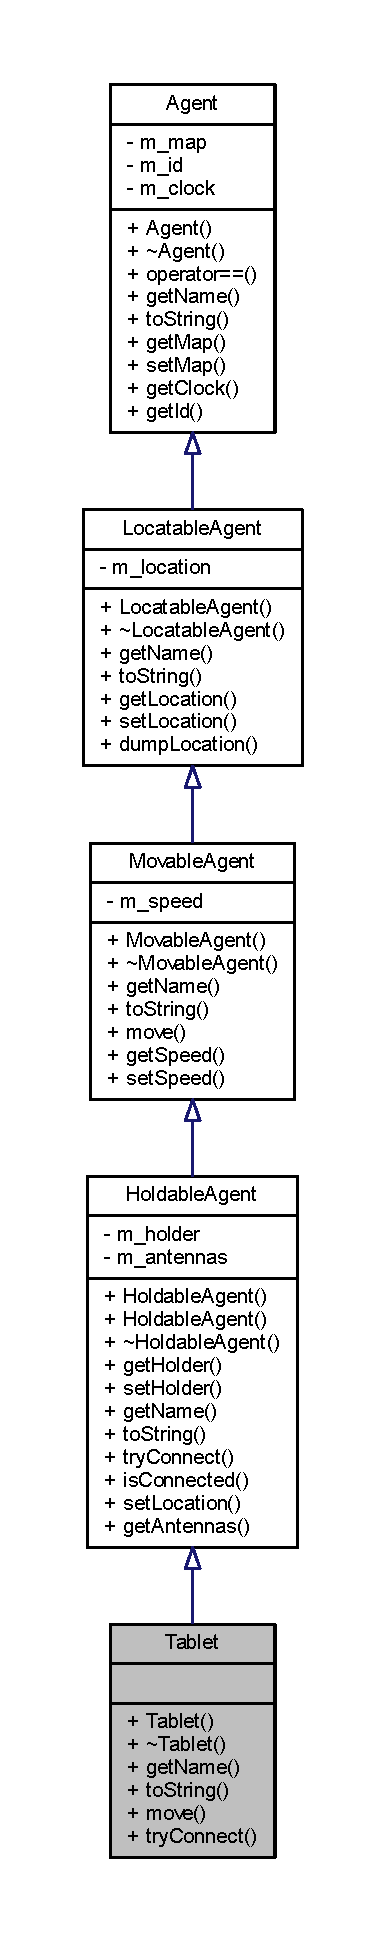
\includegraphics[height=550pt]{class_tablet__inherit__graph}
\end{center}
\end{figure}


Collaboration diagram for Tablet\+:\nopagebreak
\begin{figure}[H]
\begin{center}
\leavevmode
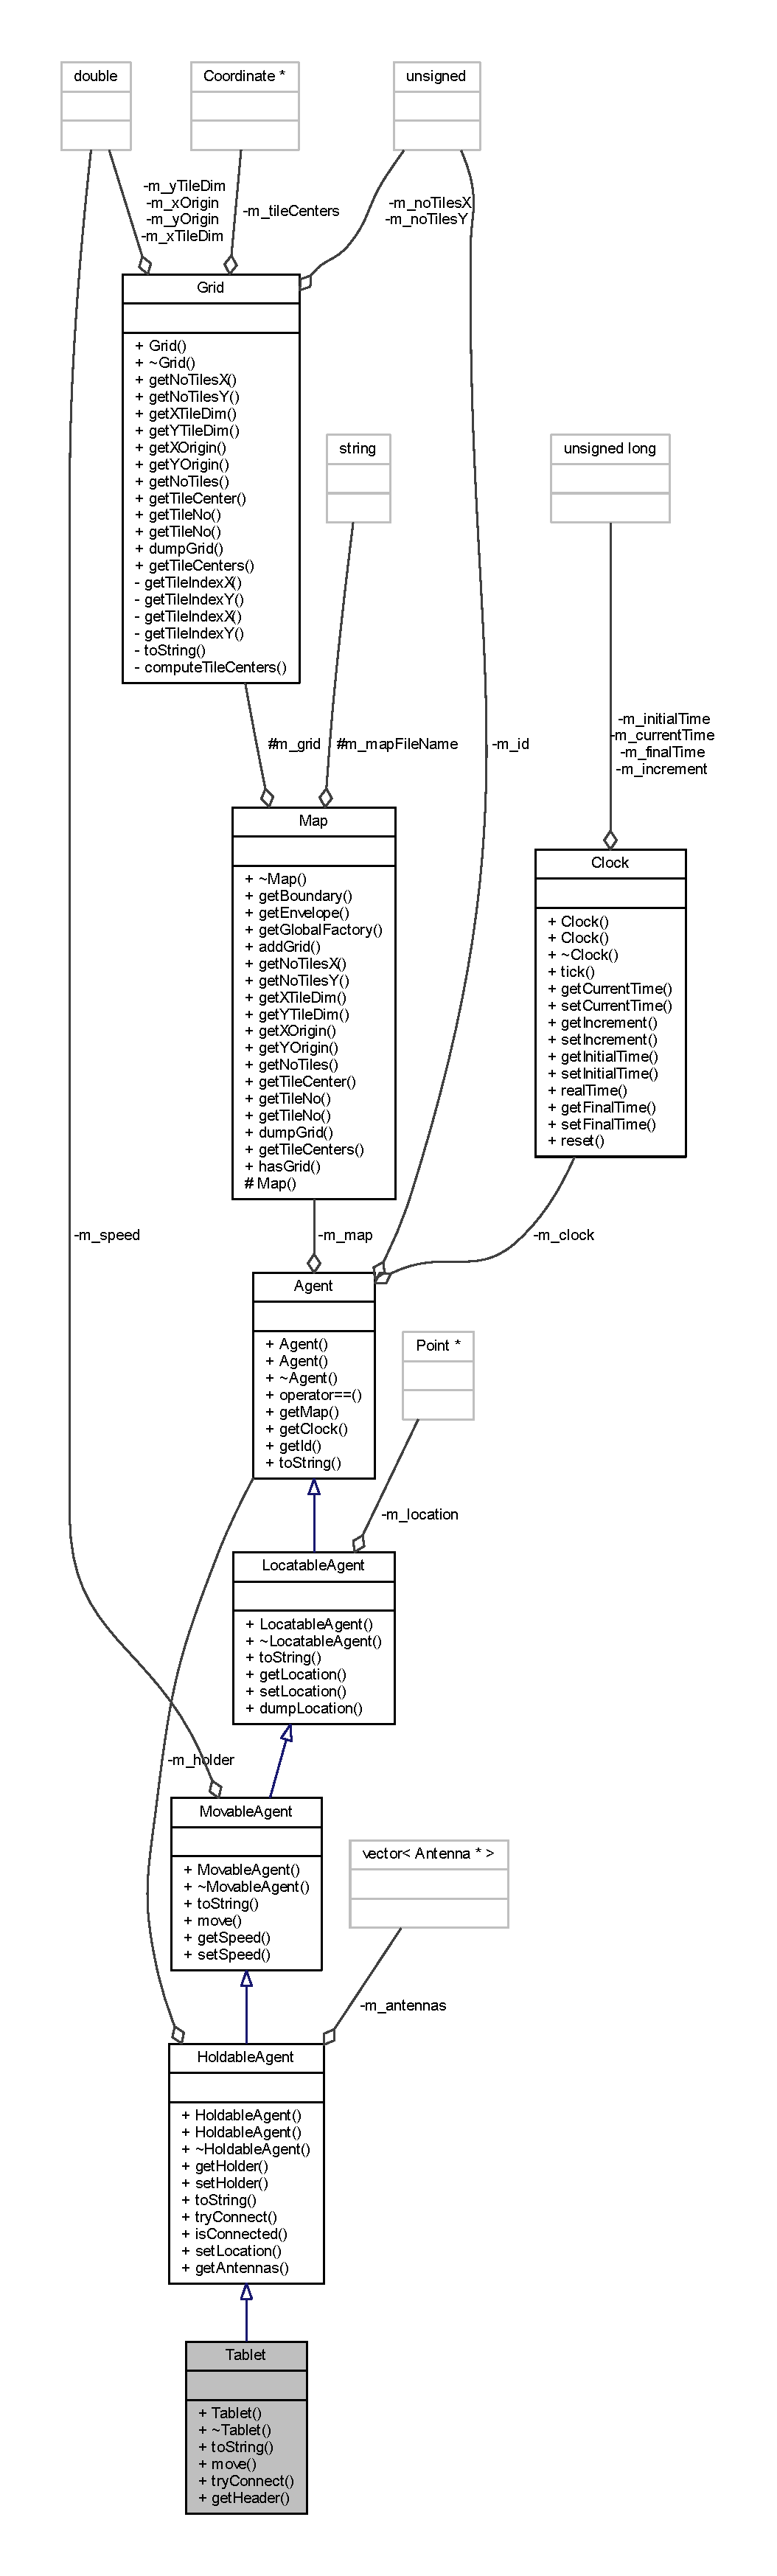
\includegraphics[height=550pt]{class_tablet__coll__graph}
\end{center}
\end{figure}
\subsection*{Public Member Functions}
\begin{DoxyCompactItemize}
\item 
\hyperlink{class_tablet_af457c0988b7a768659a284e16be58dc6}{Tablet} (const \hyperlink{class_map}{Map} $\ast$m, const unsigned long id, Point $\ast$init\+Position, const \hyperlink{class_clock}{Clock} $\ast$clock)
\item 
virtual \hyperlink{class_tablet_ac18d46eafd643e66dde81a3fefadab89}{$\sim$\+Tablet} ()
\item 
const string \hyperlink{class_tablet_adc7196aaee1e9714236b7cd8825d5826}{get\+Name} () const override
\item 
const string \hyperlink{class_tablet_a3fae01e7d526699476221c6a686a4fba}{to\+String} () const override
\item 
Point $\ast$ \hyperlink{class_tablet_ab1b8c7591be0c6ea118c8ab1c17839bb}{move} () override
\item 
bool \hyperlink{class_tablet_a2328422e1706dfeb2b51a6960e6879f0}{try\+Connect} () override
\end{DoxyCompactItemize}
\subsection*{Additional Inherited Members}


\subsection{Constructor \& Destructor Documentation}
\mbox{\Hypertarget{class_tablet_af457c0988b7a768659a284e16be58dc6}\label{class_tablet_af457c0988b7a768659a284e16be58dc6}} 
\index{Tablet@{Tablet}!Tablet@{Tablet}}
\index{Tablet@{Tablet}!Tablet@{Tablet}}
\subsubsection{\texorpdfstring{Tablet()}{Tablet()}}
{\footnotesize\ttfamily Tablet\+::\+Tablet (\begin{DoxyParamCaption}\item[{const \hyperlink{class_map}{Map} $\ast$}]{m,  }\item[{const unsigned long}]{id,  }\item[{Point $\ast$}]{init\+Position,  }\item[{const \hyperlink{class_clock}{Clock} $\ast$}]{clock }\end{DoxyParamCaption})\hspace{0.3cm}{\ttfamily [explicit]}}

Builds a new \hyperlink{class_tablet}{Tablet} object with the parameters provided by the user. 
\begin{DoxyParams}{Parameters}
{\em m} & a pointer to a \hyperlink{class_map}{Map} object used for simulation. \\
\hline
{\em id} & the id of the tablet. \\
\hline
{\em init\+Position} & the initial location on map. \\
\hline
{\em clock} & a pointer to a \hyperlink{class_clock}{Clock} object used for simulation.. \\
\hline
\end{DoxyParams}
\mbox{\Hypertarget{class_tablet_ac18d46eafd643e66dde81a3fefadab89}\label{class_tablet_ac18d46eafd643e66dde81a3fefadab89}} 
\index{Tablet@{Tablet}!````~Tablet@{$\sim$\+Tablet}}
\index{````~Tablet@{$\sim$\+Tablet}!Tablet@{Tablet}}
\subsubsection{\texorpdfstring{$\sim$\+Tablet()}{~Tablet()}}
{\footnotesize\ttfamily virtual Tablet\+::$\sim$\+Tablet (\begin{DoxyParamCaption}{ }\end{DoxyParamCaption})\hspace{0.3cm}{\ttfamily [virtual]}}

The default destructor. 

\subsection{Member Function Documentation}
\mbox{\Hypertarget{class_tablet_adc7196aaee1e9714236b7cd8825d5826}\label{class_tablet_adc7196aaee1e9714236b7cd8825d5826}} 
\index{Tablet@{Tablet}!get\+Name@{get\+Name}}
\index{get\+Name@{get\+Name}!Tablet@{Tablet}}
\subsubsection{\texorpdfstring{get\+Name()}{getName()}}
{\footnotesize\ttfamily const string Tablet\+::get\+Name (\begin{DoxyParamCaption}{ }\end{DoxyParamCaption}) const\hspace{0.3cm}{\ttfamily [override]}, {\ttfamily [virtual]}}

Returns the name of this class. \begin{DoxyReturn}{Returns}
the name of this class. 
\end{DoxyReturn}


Reimplemented from \hyperlink{class_holdable_agent_ab330bb40de51a957ef8826af629f94a2}{Holdable\+Agent}.

\mbox{\Hypertarget{class_tablet_ab1b8c7591be0c6ea118c8ab1c17839bb}\label{class_tablet_ab1b8c7591be0c6ea118c8ab1c17839bb}} 
\index{Tablet@{Tablet}!move@{move}}
\index{move@{move}!Tablet@{Tablet}}
\subsubsection{\texorpdfstring{move()}{move()}}
{\footnotesize\ttfamily Point$\ast$ Tablet\+::move (\begin{DoxyParamCaption}{ }\end{DoxyParamCaption})\hspace{0.3cm}{\ttfamily [inline]}, {\ttfamily [override]}, {\ttfamily [virtual]}}

Makes a step on the map according to an algorithm. The direction and the length of the step is determined by the displacement strategy and by the \hyperlink{class_person}{Person} object who owns this phone. The displacement strategy is set at the \hyperlink{class_person}{Person} object creation and currently two strategies are supported\+: \hyperlink{class_random_walk_displacement}{Random\+Walk\+Displacement} and \hyperlink{class_random_walk_drift_displacement}{Random\+Walk\+Drift\+Displacement}. \hyperlink{class_random_walk_displacement}{Random\+Walk\+Displacement} means that at each time instant the direction is generated as a uniformly distributed random value and the step length is computed multiplying the speed with the time interval set in the simulation configuration file. If a step projects it outside the map, it stops on the boundary. \hyperlink{class_random_walk_drift_displacement}{Random\+Walk\+Drift\+Displacement} means that there is a preference in the direction of the movement. There are two constants defined, S\+I\+M\+\_\+\+T\+R\+E\+N\+D\+\_\+\+A\+N\+G\+L\+E\+\_\+1 and S\+I\+M\+\_\+\+T\+R\+E\+N\+D\+\_\+\+A\+N\+G\+L\+E\+\_\+2 (3\+P\+I/4 and 5\+P\+I/4), and in the first half of the simulation the direction is generated as a normal distributed random value with the mean equals to S\+I\+M\+\_\+\+T\+R\+E\+N\+D\+\_\+\+A\+N\+G\+L\+E\+\_\+1 and sd = 0.\+1 while during the second half of the simulation it is generated as a normal distributed random value with the mean equals to S\+I\+M\+\_\+\+T\+R\+E\+N\+D\+\_\+\+A\+N\+G\+L\+E\+\_\+2 and the same sd. Again, any kind of \hyperlink{class_movable_agent}{Movable\+Agent} can only move inside the map boundary. If a step projects it outside the map, it stops on the boundary. \begin{DoxyReturn}{Returns}
the final location after the displacement. 
\end{DoxyReturn}


Implements \hyperlink{class_movable_agent_a88b617f0e78c817634e5b587da045ab0}{Movable\+Agent}.

Here is the call graph for this function\+:\nopagebreak
\begin{figure}[H]
\begin{center}
\leavevmode
\includegraphics[width=327pt]{class_tablet_ab1b8c7591be0c6ea118c8ab1c17839bb_cgraph}
\end{center}
\end{figure}
\mbox{\Hypertarget{class_tablet_a3fae01e7d526699476221c6a686a4fba}\label{class_tablet_a3fae01e7d526699476221c6a686a4fba}} 
\index{Tablet@{Tablet}!to\+String@{to\+String}}
\index{to\+String@{to\+String}!Tablet@{Tablet}}
\subsubsection{\texorpdfstring{to\+String()}{toString()}}
{\footnotesize\ttfamily const string Tablet\+::to\+String (\begin{DoxyParamCaption}{ }\end{DoxyParamCaption}) const\hspace{0.3cm}{\ttfamily [override]}, {\ttfamily [virtual]}}

Builds a human readable representation of this class. \begin{DoxyReturn}{Returns}
a human readable representation of this class. 
\end{DoxyReturn}


Reimplemented from \hyperlink{class_holdable_agent_a2c581226b8994f24b6b2306ae17dbb52}{Holdable\+Agent}.

\mbox{\Hypertarget{class_tablet_a2328422e1706dfeb2b51a6960e6879f0}\label{class_tablet_a2328422e1706dfeb2b51a6960e6879f0}} 
\index{Tablet@{Tablet}!try\+Connect@{try\+Connect}}
\index{try\+Connect@{try\+Connect}!Tablet@{Tablet}}
\subsubsection{\texorpdfstring{try\+Connect()}{tryConnect()}}
{\footnotesize\ttfamily bool Tablet\+::try\+Connect (\begin{DoxyParamCaption}{ }\end{DoxyParamCaption})\hspace{0.3cm}{\ttfamily [override]}, {\ttfamily [virtual]}}

Called after the tablet changes location on the map, tries to connect to an antenna. \begin{DoxyReturn}{Returns}
true if the connection succeeds, false otherwise. 
\end{DoxyReturn}


Implements \hyperlink{class_holdable_agent_a0789d757d81b43ee016e9362046f6dea}{Holdable\+Agent}.

Here is the caller graph for this function\+:\nopagebreak
\begin{figure}[H]
\begin{center}
\leavevmode
\includegraphics[width=283pt]{class_tablet_a2328422e1706dfeb2b51a6960e6879f0_icgraph}
\end{center}
\end{figure}


The documentation for this class was generated from the following file\+:\begin{DoxyCompactItemize}
\item 
include/\hyperlink{_tablet_8h}{Tablet.\+h}\end{DoxyCompactItemize}

\section{World Class Reference}
\label{class_world}\index{World@{World}}


{\ttfamily \#include $<$World.\+h$>$}

\subsection*{Public Member Functions}
\begin{DoxyCompactItemize}
\item 
\textbf{ World} (\textbf{ Map} $\ast$map, int num\+Persons, int num\+Antennas, int num\+Mobile\+Phones)
\item 
\textbf{ World} (\textbf{ Map} $\ast$map, int num\+Persons, const string \&config\+Antennas\+File, int num\+Mobile\+Phones) noexcept(false)
\item 
\textbf{ World} (\textbf{ Map} $\ast$map, const string \&config\+Persons\+File\+Name, const string \&config\+Antennas\+File\+Name, const string \&config\+Simulation\+File\+Name) noexcept(false)
\item 
virtual \textbf{ $\sim$\+World} ()
\item 
void \textbf{ run\+Simulation} (string \&persons\+File, string \&antennas\+File) noexcept(false)
\item 
void \textbf{ dump\+State} ()
\item 
unsigned int \textbf{ get\+Current\+Time} ()
\item 
\textbf{ Agents\+Collection} $\ast$ \textbf{ get\+Agents} () const
\item 
void \textbf{ set\+Agents} (\textbf{ Agents\+Collection} $\ast$agents)
\item 
\textbf{ Clock} $\ast$ \textbf{ get\+Clock} () const
\item 
void \textbf{ set\+Clock} (\textbf{ Clock} $\ast$clock)
\item 
\textbf{ Map} $\ast$ \textbf{ get\+Map} () const
\item 
void \textbf{ set\+Map} (\textbf{ Map} $\ast$map)
\end{DoxyCompactItemize}
\subsection*{Private Member Functions}
\begin{DoxyCompactItemize}
\item 
vector$<$ \textbf{ Person} $\ast$ $>$ \textbf{ generate\+Population} (unsigned long num\+Persons)
\item 
vector$<$ \textbf{ Person} $\ast$ $>$ \textbf{ generate\+Population} (unsigned long num\+Persons, vector$<$ double $>$ params, \textbf{ Person\+::\+Age\+Distributions} age\+\_\+distribution, double male\+\_\+share, double prob\+\_\+mobile\+\_\+phone, double speed\+\_\+walk, double speed\+\_\+car)
\item 
vector$<$ \textbf{ Antenna} $\ast$ $>$ \textbf{ generate\+Antennas} (unsigned long num\+Antennas)
\item 
vector$<$ \textbf{ Antenna} $\ast$ $>$ \textbf{ parse\+Antennas} (const string \&config\+Antennas\+File) noexcept(false)
\item 
vector$<$ \textbf{ Person} $\ast$ $>$ \textbf{ parse\+Persons} (const string \&persons\+File\+Name) noexcept(false)
\item 
vector$<$ \textbf{ Mobile\+Phone} $\ast$ $>$ \textbf{ generate\+Mobile\+Phones} (int num\+Mobile\+Phones, \textbf{ Holdable\+Agent\+::\+C\+O\+N\+N\+E\+C\+T\+I\+O\+N\+\_\+\+T\+Y\+PE} conn\+Type)
\item 
void \textbf{ parse\+Simulation\+File} (const string \&config\+Simulation\+File\+Name) noexcept(false)
\end{DoxyCompactItemize}
\subsection*{Private Attributes}
\begin{DoxyCompactItemize}
\item 
\textbf{ Map} $\ast$ \textbf{ m\+\_\+map}
\item 
\textbf{ Agents\+Collection} $\ast$ \textbf{ m\+\_\+agents\+Collection}
\item 
\textbf{ Clock} $\ast$ \textbf{ m\+\_\+clock}
\item 
unsigned long \textbf{ m\+\_\+start\+Time}
\item 
unsigned long \textbf{ m\+\_\+end\+Time}
\item 
unsigned long \textbf{ m\+\_\+time\+Increment}
\item 
\textbf{ Holdable\+Agent\+::\+C\+O\+N\+N\+E\+C\+T\+I\+O\+N\+\_\+\+T\+Y\+PE} \textbf{ m\+\_\+conn\+Type}
\item 
\textbf{ Movement\+Type} \textbf{ m\+\_\+mv\+Type}
\end{DoxyCompactItemize}


\subsection{Detailed Description}


Definition at line 28 of file World.\+h.



\subsection{Constructor \& Destructor Documentation}
\mbox{\label{class_world_a94871f094bb3eabb67f5bd1b10396832}} 
\index{World@{World}!World@{World}}
\index{World@{World}!World@{World}}
\subsubsection{World()\hspace{0.1cm}{\footnotesize\ttfamily [1/3]}}
{\footnotesize\ttfamily World\+::\+World (\begin{DoxyParamCaption}\item[{\textbf{ Map} $\ast$}]{map,  }\item[{int}]{num\+Persons,  }\item[{int}]{num\+Antennas,  }\item[{int}]{num\+Mobile\+Phones }\end{DoxyParamCaption})}

Default constructor 

Definition at line 37 of file World.\+cpp.

\mbox{\label{class_world_a5a02572c10d750037a8c604a7d806550}} 
\index{World@{World}!World@{World}}
\index{World@{World}!World@{World}}
\subsubsection{World()\hspace{0.1cm}{\footnotesize\ttfamily [2/3]}}
{\footnotesize\ttfamily World\+::\+World (\begin{DoxyParamCaption}\item[{\textbf{ Map} $\ast$}]{map,  }\item[{int}]{num\+Persons,  }\item[{const string \&}]{config\+Antennas\+File,  }\item[{int}]{num\+Mobile\+Phones }\end{DoxyParamCaption})\hspace{0.3cm}{\ttfamily [noexcept]}}



Definition at line 61 of file World.\+cpp.

\mbox{\label{class_world_a6376bd8ac7c88b8e01e7cca06d9bb18a}} 
\index{World@{World}!World@{World}}
\index{World@{World}!World@{World}}
\subsubsection{World()\hspace{0.1cm}{\footnotesize\ttfamily [3/3]}}
{\footnotesize\ttfamily World\+::\+World (\begin{DoxyParamCaption}\item[{\textbf{ Map} $\ast$}]{map,  }\item[{const string \&}]{config\+Persons\+File\+Name,  }\item[{const string \&}]{config\+Antennas\+File\+Name,  }\item[{const string \&}]{config\+Simulation\+File\+Name }\end{DoxyParamCaption})\hspace{0.3cm}{\ttfamily [noexcept]}}



Definition at line 84 of file World.\+cpp.

\mbox{\label{class_world_a8c73fba541a5817fff65147ba47cd827}} 
\index{World@{World}!````~World@{$\sim$World}}
\index{````~World@{$\sim$World}!World@{World}}
\subsubsection{$\sim$World()}
{\footnotesize\ttfamily World\+::$\sim$\+World (\begin{DoxyParamCaption}{ }\end{DoxyParamCaption})\hspace{0.3cm}{\ttfamily [virtual]}}

Default destructor 

Definition at line 104 of file World.\+cpp.



References m\+\_\+agents\+Collection, and m\+\_\+clock.



\subsection{Member Function Documentation}
\mbox{\label{class_world_abb6faf5385d3960dca29ee9390460eea}} 
\index{World@{World}!dumpState@{dumpState}}
\index{dumpState@{dumpState}!World@{World}}
\subsubsection{dumpState()}
{\footnotesize\ttfamily void World\+::dump\+State (\begin{DoxyParamCaption}{ }\end{DoxyParamCaption})}

\mbox{\label{class_world_a6cb3aa7d814b3d6302ea984889179eac}} 
\index{World@{World}!generateAntennas@{generateAntennas}}
\index{generateAntennas@{generateAntennas}!World@{World}}
\subsubsection{generateAntennas()}
{\footnotesize\ttfamily vector$<$ \textbf{ Antenna} $\ast$ $>$ World\+::generate\+Antennas (\begin{DoxyParamCaption}\item[{unsigned long}]{num\+Antennas }\end{DoxyParamCaption})\hspace{0.3cm}{\ttfamily [private]}}



Definition at line 208 of file World.\+cpp.



References Constants\+::\+A\+N\+T\+E\+N\+N\+A\+\_\+\+P\+O\+W\+ER, Constants\+::\+A\+T\+T\+\_\+\+F\+A\+C\+T\+OR, utils\+::generate\+Points(), get\+Map(), I\+D\+Generator\+::instance(), m\+\_\+clock, Constants\+::\+M\+A\+X\+\_\+\+C\+O\+N\+N\+E\+C\+T\+I\+O\+NS, I\+D\+Generator\+::next(), O\+M\+N\+I\+D\+I\+R\+E\+C\+T\+I\+O\+N\+AL, Constants\+::\+S\+\_\+\+M\+ID, and Constants\+::\+S\+\_\+\+S\+T\+E\+EP.

\mbox{\label{class_world_a478f62a296d9a7b6587c116aab6563c6}} 
\index{World@{World}!generateMobilePhones@{generateMobilePhones}}
\index{generateMobilePhones@{generateMobilePhones}!World@{World}}
\subsubsection{generateMobilePhones()}
{\footnotesize\ttfamily vector$<$ \textbf{ Mobile\+Phone} $\ast$ $>$ World\+::generate\+Mobile\+Phones (\begin{DoxyParamCaption}\item[{int}]{num\+Mobile\+Phones,  }\item[{\textbf{ Holdable\+Agent\+::\+C\+O\+N\+N\+E\+C\+T\+I\+O\+N\+\_\+\+T\+Y\+PE}}]{conn\+Type }\end{DoxyParamCaption})\hspace{0.3cm}{\ttfamily [private]}}



Definition at line 228 of file World.\+cpp.



References Agents\+Collection\+::add\+Agent(), get\+Map(), I\+D\+Generator\+::instance(), m\+\_\+agents\+Collection, m\+\_\+clock, I\+D\+Generator\+::next(), Constants\+::\+P\+O\+W\+E\+R\+\_\+\+T\+H\+R\+E\+S\+H\+O\+LD, and Constants\+::\+Q\+U\+A\+L\+I\+T\+Y\+\_\+\+T\+H\+R\+E\+S\+H\+O\+LD.



Referenced by generate\+Population().

\mbox{\label{class_world_a76bc2ffba54afefbb84b2f6fc781b629}} 
\index{World@{World}!generatePopulation@{generatePopulation}}
\index{generatePopulation@{generatePopulation}!World@{World}}
\subsubsection{generatePopulation()\hspace{0.1cm}{\footnotesize\ttfamily [1/2]}}
{\footnotesize\ttfamily vector$<$ \textbf{ Person} $\ast$ $>$ World\+::generate\+Population (\begin{DoxyParamCaption}\item[{unsigned long}]{num\+Persons }\end{DoxyParamCaption})\hspace{0.3cm}{\ttfamily [private]}}



Definition at line 189 of file World.\+cpp.



References Random\+Number\+Generator\+::generate\+Normal2\+Double(), utils\+::generate\+Points(), Random\+Number\+Generator\+::generate\+Uniform\+Int(), get\+Map(), I\+D\+Generator\+::instance(), Random\+Number\+Generator\+::instance(), m\+\_\+clock, and I\+D\+Generator\+::next().

\mbox{\label{class_world_ac6bb92d77d6be53323a24b0fd825f986}} 
\index{World@{World}!generatePopulation@{generatePopulation}}
\index{generatePopulation@{generatePopulation}!World@{World}}
\subsubsection{generatePopulation()\hspace{0.1cm}{\footnotesize\ttfamily [2/2]}}
{\footnotesize\ttfamily vector$<$ \textbf{ Person} $\ast$ $>$ World\+::generate\+Population (\begin{DoxyParamCaption}\item[{unsigned long}]{num\+Persons,  }\item[{vector$<$ double $>$}]{params,  }\item[{\textbf{ Person\+::\+Age\+Distributions}}]{age\+\_\+distribution,  }\item[{double}]{male\+\_\+share,  }\item[{double}]{prob\+\_\+mobile\+\_\+phone,  }\item[{double}]{speed\+\_\+walk,  }\item[{double}]{speed\+\_\+car }\end{DoxyParamCaption})\hspace{0.3cm}{\ttfamily [private]}}



Definition at line 364 of file World.\+cpp.



References Person\+::add\+Device(), Random\+Number\+Generator\+::generate\+Binomial\+Int(), generate\+Mobile\+Phones(), Random\+Number\+Generator\+::generate\+Normal\+Double(), utils\+::generate\+Points(), Random\+Number\+Generator\+::generate\+Truncated\+Normal\+Double(), Random\+Number\+Generator\+::generate\+Uniform\+Double(), get\+Map(), I\+D\+Generator\+::instance(), Random\+Number\+Generator\+::instance(), m\+\_\+clock, m\+\_\+conn\+Type, and I\+D\+Generator\+::next().

\mbox{\label{class_world_a365cced3803fd8390a781619b61e2818}} 
\index{World@{World}!getAgents@{getAgents}}
\index{getAgents@{getAgents}!World@{World}}
\subsubsection{getAgents()}
{\footnotesize\ttfamily \textbf{ Agents\+Collection} $\ast$ World\+::get\+Agents (\begin{DoxyParamCaption}{ }\end{DoxyParamCaption}) const}



Definition at line 165 of file World.\+cpp.



References m\+\_\+agents\+Collection.

\mbox{\label{class_world_a521915088db371c5730093331a74b080}} 
\index{World@{World}!getClock@{getClock}}
\index{getClock@{getClock}!World@{World}}
\subsubsection{getClock()}
{\footnotesize\ttfamily \textbf{ Clock} $\ast$ World\+::get\+Clock (\begin{DoxyParamCaption}{ }\end{DoxyParamCaption}) const}



Definition at line 173 of file World.\+cpp.



References m\+\_\+clock.

\mbox{\label{class_world_af33b51dff9edc6770890ef579700d959}} 
\index{World@{World}!getCurrentTime@{getCurrentTime}}
\index{getCurrentTime@{getCurrentTime}!World@{World}}
\subsubsection{getCurrentTime()}
{\footnotesize\ttfamily unsigned int World\+::get\+Current\+Time (\begin{DoxyParamCaption}{ }\end{DoxyParamCaption})}



Definition at line 161 of file World.\+cpp.



References Clock\+::get\+Current\+Time(), and m\+\_\+clock.

\mbox{\label{class_world_a5b82e6105d8f4b3d757eb7da6d65205a}} 
\index{World@{World}!getMap@{getMap}}
\index{getMap@{getMap}!World@{World}}
\subsubsection{getMap()}
{\footnotesize\ttfamily \textbf{ Map} $\ast$ World\+::get\+Map (\begin{DoxyParamCaption}{ }\end{DoxyParamCaption}) const}



Definition at line 181 of file World.\+cpp.



References m\+\_\+map.



Referenced by generate\+Antennas(), generate\+Mobile\+Phones(), and generate\+Population().

\mbox{\label{class_world_aaf31e06b9b5a40a4338164e0f641f7d0}} 
\index{World@{World}!parseAntennas@{parseAntennas}}
\index{parseAntennas@{parseAntennas}!World@{World}}
\subsubsection{parseAntennas()}
{\footnotesize\ttfamily vector$<$ \textbf{ Antenna} $\ast$ $>$ World\+::parse\+Antennas (\begin{DoxyParamCaption}\item[{const string \&}]{config\+Antennas\+File }\end{DoxyParamCaption})\hspace{0.3cm}{\ttfamily [private]}, {\ttfamily [noexcept]}}



Definition at line 240 of file World.\+cpp.



References tinyxml2\+::\+X\+M\+L\+Node\+::\+First\+Child\+Element(), utils\+::get\+First\+Child\+Element(), I\+D\+Generator\+::instance(), tinyxml2\+::\+X\+M\+L\+Document\+::\+Load\+File(), tinyxml2\+::\+X\+M\+L\+Element\+::\+Name(), I\+D\+Generator\+::next(), tinyxml2\+::\+X\+M\+L\+Node\+::\+Next\+Sibling\+Element(), and tinyxml2\+::\+X\+M\+L\+\_\+\+S\+U\+C\+C\+E\+SS.

\mbox{\label{class_world_a8bdce1dbc8d7a653d63a59674e283622}} 
\index{World@{World}!parsePersons@{parsePersons}}
\index{parsePersons@{parsePersons}!World@{World}}
\subsubsection{parsePersons()}
{\footnotesize\ttfamily vector$<$ \textbf{ Person} $\ast$ $>$ World\+::parse\+Persons (\begin{DoxyParamCaption}\item[{const string \&}]{persons\+File\+Name }\end{DoxyParamCaption})\hspace{0.3cm}{\ttfamily [private]}, {\ttfamily [noexcept]}}



Definition at line 265 of file World.\+cpp.



References tinyxml2\+::\+X\+M\+L\+Node\+::\+First\+Child\+Element(), utils\+::get\+First\+Child\+Element(), utils\+::get\+Node(), tinyxml2\+::\+X\+M\+L\+Document\+::\+Load\+File(), tinyxml2\+::\+X\+M\+L\+Node\+::\+To\+Text(), tinyxml2\+::\+X\+M\+L\+Node\+::\+Value(), and tinyxml2\+::\+X\+M\+L\+\_\+\+S\+U\+C\+C\+E\+SS.

\mbox{\label{class_world_a7f00dc79cc98281dbf7c51fb2c83e8d6}} 
\index{World@{World}!parseSimulationFile@{parseSimulationFile}}
\index{parseSimulationFile@{parseSimulationFile}!World@{World}}
\subsubsection{parseSimulationFile()}
{\footnotesize\ttfamily void World\+::parse\+Simulation\+File (\begin{DoxyParamCaption}\item[{const string \&}]{config\+Simulation\+File\+Name }\end{DoxyParamCaption})\hspace{0.3cm}{\ttfamily [private]}, {\ttfamily [noexcept]}}



Definition at line 331 of file World.\+cpp.



References tinyxml2\+::\+X\+M\+L\+Node\+::\+First\+Child\+Element(), utils\+::get\+Node(), tinyxml2\+::\+X\+M\+L\+Document\+::\+Load\+File(), R\+A\+N\+D\+O\+M\+\_\+\+W\+A\+LK, tinyxml2\+::\+X\+M\+L\+Node\+::\+To\+Text(), U\+N\+K\+N\+O\+WN, tinyxml2\+::\+X\+M\+L\+Node\+::\+Value(), and tinyxml2\+::\+X\+M\+L\+\_\+\+S\+U\+C\+C\+E\+SS.

\mbox{\label{class_world_af8d69e177beec5a9cf3c200f292db7db}} 
\index{World@{World}!runSimulation@{runSimulation}}
\index{runSimulation@{runSimulation}!World@{World}}
\subsubsection{runSimulation()}
{\footnotesize\ttfamily void World\+::run\+Simulation (\begin{DoxyParamCaption}\item[{string \&}]{persons\+File,  }\item[{string \&}]{antennas\+File }\end{DoxyParamCaption})\hspace{0.3cm}{\ttfamily [noexcept]}}



Definition at line 111 of file World.\+cpp.



References Person\+::dump\+Devices(), Locatable\+Agent\+::dump\+Location(), and Person\+::move().

\mbox{\label{class_world_afa8e5c2943c72aa664590abbb024896b}} 
\index{World@{World}!setAgents@{setAgents}}
\index{setAgents@{setAgents}!World@{World}}
\subsubsection{setAgents()}
{\footnotesize\ttfamily void World\+::set\+Agents (\begin{DoxyParamCaption}\item[{\textbf{ Agents\+Collection} $\ast$}]{agents }\end{DoxyParamCaption})}



Definition at line 169 of file World.\+cpp.



References m\+\_\+agents\+Collection.

\mbox{\label{class_world_a52ebe3eed240fe4dd37915a1dad02efd}} 
\index{World@{World}!setClock@{setClock}}
\index{setClock@{setClock}!World@{World}}
\subsubsection{setClock()}
{\footnotesize\ttfamily void World\+::set\+Clock (\begin{DoxyParamCaption}\item[{\textbf{ Clock} $\ast$}]{clock }\end{DoxyParamCaption})}



Definition at line 177 of file World.\+cpp.



References m\+\_\+clock.

\mbox{\label{class_world_a9dc80487d5c2d1d4f2af0c1d7f015204}} 
\index{World@{World}!setMap@{setMap}}
\index{setMap@{setMap}!World@{World}}
\subsubsection{setMap()}
{\footnotesize\ttfamily void World\+::set\+Map (\begin{DoxyParamCaption}\item[{\textbf{ Map} $\ast$}]{map }\end{DoxyParamCaption})}



Definition at line 185 of file World.\+cpp.



References m\+\_\+map.



\subsection{Member Data Documentation}
\mbox{\label{class_world_ae1262689381f00828c0a639b7cbb52a3}} 
\index{World@{World}!m\_agentsCollection@{m\_agentsCollection}}
\index{m\_agentsCollection@{m\_agentsCollection}!World@{World}}
\subsubsection{m\_agentsCollection}
{\footnotesize\ttfamily \textbf{ Agents\+Collection}$\ast$ World\+::m\+\_\+agents\+Collection\hspace{0.3cm}{\ttfamily [private]}}



Definition at line 60 of file World.\+h.



Referenced by generate\+Mobile\+Phones(), get\+Agents(), set\+Agents(), and $\sim$\+World().

\mbox{\label{class_world_a8359eb424f01e41703faa0885a4414bf}} 
\index{World@{World}!m\_clock@{m\_clock}}
\index{m\_clock@{m\_clock}!World@{World}}
\subsubsection{m\_clock}
{\footnotesize\ttfamily \textbf{ Clock}$\ast$ World\+::m\+\_\+clock\hspace{0.3cm}{\ttfamily [private]}}



Definition at line 61 of file World.\+h.



Referenced by generate\+Antennas(), generate\+Mobile\+Phones(), generate\+Population(), get\+Clock(), get\+Current\+Time(), set\+Clock(), and $\sim$\+World().

\mbox{\label{class_world_afeac65cddcd1e1c4fa14a17efa35be06}} 
\index{World@{World}!m\_connType@{m\_connType}}
\index{m\_connType@{m\_connType}!World@{World}}
\subsubsection{m\_connType}
{\footnotesize\ttfamily \textbf{ Holdable\+Agent\+::\+C\+O\+N\+N\+E\+C\+T\+I\+O\+N\+\_\+\+T\+Y\+PE} World\+::m\+\_\+conn\+Type\hspace{0.3cm}{\ttfamily [private]}}



Definition at line 66 of file World.\+h.



Referenced by generate\+Population().

\mbox{\label{class_world_ab6b8ad11e4031f3072a78f00a66e9ec5}} 
\index{World@{World}!m\_endTime@{m\_endTime}}
\index{m\_endTime@{m\_endTime}!World@{World}}
\subsubsection{m\_endTime}
{\footnotesize\ttfamily unsigned long World\+::m\+\_\+end\+Time\hspace{0.3cm}{\ttfamily [private]}}



Definition at line 63 of file World.\+h.

\mbox{\label{class_world_ae1e6f62c5b282e94ffdcaab58fcb3fb4}} 
\index{World@{World}!m\_map@{m\_map}}
\index{m\_map@{m\_map}!World@{World}}
\subsubsection{m\_map}
{\footnotesize\ttfamily \textbf{ Map}$\ast$ World\+::m\+\_\+map\hspace{0.3cm}{\ttfamily [private]}}



Definition at line 58 of file World.\+h.



Referenced by get\+Map(), and set\+Map().

\mbox{\label{class_world_a9fcf012ce7262edf5646f0720ffd7666}} 
\index{World@{World}!m\_mvType@{m\_mvType}}
\index{m\_mvType@{m\_mvType}!World@{World}}
\subsubsection{m\_mvType}
{\footnotesize\ttfamily \textbf{ Movement\+Type} World\+::m\+\_\+mv\+Type\hspace{0.3cm}{\ttfamily [private]}}



Definition at line 67 of file World.\+h.

\mbox{\label{class_world_a5b46814e7da7222730be62154bf10008}} 
\index{World@{World}!m\_startTime@{m\_startTime}}
\index{m\_startTime@{m\_startTime}!World@{World}}
\subsubsection{m\_startTime}
{\footnotesize\ttfamily unsigned long World\+::m\+\_\+start\+Time\hspace{0.3cm}{\ttfamily [private]}}



Definition at line 62 of file World.\+h.

\mbox{\label{class_world_a97f773548fef49eb408115c097aa995d}} 
\index{World@{World}!m\_timeIncrement@{m\_timeIncrement}}
\index{m\_timeIncrement@{m\_timeIncrement}!World@{World}}
\subsubsection{m\_timeIncrement}
{\footnotesize\ttfamily unsigned long World\+::m\+\_\+time\+Increment\hspace{0.3cm}{\ttfamily [private]}}



Definition at line 64 of file World.\+h.



The documentation for this class was generated from the following files\+:\begin{DoxyCompactItemize}
\item 
include/\textbf{ World.\+h}\item 
src/\textbf{ World.\+cpp}\end{DoxyCompactItemize}

\section{tinyxml2\+::X\+M\+L\+Attribute Class Reference}
\label{classtinyxml2_1_1_x_m_l_attribute}\index{tinyxml2::XMLAttribute@{tinyxml2::XMLAttribute}}


{\ttfamily \#include $<$tinyxml2.\+h$>$}

\subsection*{Public Member Functions}
\begin{DoxyCompactItemize}
\item 
const char $\ast$ \textbf{ Name} () const
\begin{DoxyCompactList}\small\item\em The name of the attribute. \end{DoxyCompactList}\item 
const char $\ast$ \textbf{ Value} () const
\begin{DoxyCompactList}\small\item\em The value of the attribute. \end{DoxyCompactList}\item 
int \textbf{ Get\+Line\+Num} () const
\begin{DoxyCompactList}\small\item\em Gets the line number the attribute is in, if the document was parsed from a file. \end{DoxyCompactList}\item 
const \textbf{ X\+M\+L\+Attribute} $\ast$ \textbf{ Next} () const
\begin{DoxyCompactList}\small\item\em The next attribute in the list. \end{DoxyCompactList}\item 
int \textbf{ Int\+Value} () const
\item 
int64\+\_\+t \textbf{ Int64\+Value} () const
\item 
unsigned \textbf{ Unsigned\+Value} () const
\begin{DoxyCompactList}\small\item\em Query as an unsigned integer. See \doxyref{Int\+Value()}{p.}{classtinyxml2_1_1_x_m_l_attribute_adfa2433f0fdafd5c3880936de9affa80} \end{DoxyCompactList}\item 
bool \textbf{ Bool\+Value} () const
\begin{DoxyCompactList}\small\item\em Query as a boolean. See \doxyref{Int\+Value()}{p.}{classtinyxml2_1_1_x_m_l_attribute_adfa2433f0fdafd5c3880936de9affa80} \end{DoxyCompactList}\item 
double \textbf{ Double\+Value} () const
\begin{DoxyCompactList}\small\item\em Query as a double. See \doxyref{Int\+Value()}{p.}{classtinyxml2_1_1_x_m_l_attribute_adfa2433f0fdafd5c3880936de9affa80} \end{DoxyCompactList}\item 
float \textbf{ Float\+Value} () const
\begin{DoxyCompactList}\small\item\em Query as a float. See \doxyref{Int\+Value()}{p.}{classtinyxml2_1_1_x_m_l_attribute_adfa2433f0fdafd5c3880936de9affa80} \end{DoxyCompactList}\item 
\textbf{ X\+M\+L\+Error} \textbf{ Query\+Int\+Value} (int $\ast$value) const
\item 
\textbf{ X\+M\+L\+Error} \textbf{ Query\+Unsigned\+Value} (unsigned int $\ast$value) const
\begin{DoxyCompactList}\small\item\em See Query\+Int\+Value. \end{DoxyCompactList}\item 
\textbf{ X\+M\+L\+Error} \textbf{ Query\+Int64\+Value} (int64\+\_\+t $\ast$value) const
\begin{DoxyCompactList}\small\item\em See Query\+Int\+Value. \end{DoxyCompactList}\item 
\textbf{ X\+M\+L\+Error} \textbf{ Query\+Bool\+Value} (bool $\ast$value) const
\begin{DoxyCompactList}\small\item\em See Query\+Int\+Value. \end{DoxyCompactList}\item 
\textbf{ X\+M\+L\+Error} \textbf{ Query\+Double\+Value} (double $\ast$value) const
\begin{DoxyCompactList}\small\item\em See Query\+Int\+Value. \end{DoxyCompactList}\item 
\textbf{ X\+M\+L\+Error} \textbf{ Query\+Float\+Value} (float $\ast$value) const
\begin{DoxyCompactList}\small\item\em See Query\+Int\+Value. \end{DoxyCompactList}\item 
void \textbf{ Set\+Attribute} (const char $\ast$value)
\begin{DoxyCompactList}\small\item\em Set the attribute to a string value. \end{DoxyCompactList}\item 
void \textbf{ Set\+Attribute} (int value)
\begin{DoxyCompactList}\small\item\em Set the attribute to value. \end{DoxyCompactList}\item 
void \textbf{ Set\+Attribute} (unsigned value)
\begin{DoxyCompactList}\small\item\em Set the attribute to value. \end{DoxyCompactList}\item 
void \textbf{ Set\+Attribute} (int64\+\_\+t value)
\begin{DoxyCompactList}\small\item\em Set the attribute to value. \end{DoxyCompactList}\item 
void \textbf{ Set\+Attribute} (bool value)
\begin{DoxyCompactList}\small\item\em Set the attribute to value. \end{DoxyCompactList}\item 
void \textbf{ Set\+Attribute} (double value)
\begin{DoxyCompactList}\small\item\em Set the attribute to value. \end{DoxyCompactList}\item 
void \textbf{ Set\+Attribute} (float value)
\begin{DoxyCompactList}\small\item\em Set the attribute to value. \end{DoxyCompactList}\end{DoxyCompactItemize}
\subsection*{Private Types}
\begin{DoxyCompactItemize}
\item 
enum \{ \textbf{ B\+U\+F\+\_\+\+S\+I\+ZE} = 200
 \}
\end{DoxyCompactItemize}
\subsection*{Private Member Functions}
\begin{DoxyCompactItemize}
\item 
\textbf{ X\+M\+L\+Attribute} ()
\item 
virtual \textbf{ $\sim$\+X\+M\+L\+Attribute} ()
\item 
\textbf{ X\+M\+L\+Attribute} (const \textbf{ X\+M\+L\+Attribute} \&)
\item 
void \textbf{ operator=} (const \textbf{ X\+M\+L\+Attribute} \&)
\item 
void \textbf{ Set\+Name} (const char $\ast$name)
\item 
char $\ast$ \textbf{ Parse\+Deep} (char $\ast$p, bool process\+Entities, int $\ast$cur\+Line\+Num\+Ptr)
\end{DoxyCompactItemize}
\subsection*{Private Attributes}
\begin{DoxyCompactItemize}
\item 
\textbf{ Str\+Pair} \textbf{ \+\_\+name}
\item 
\textbf{ Str\+Pair} \textbf{ \+\_\+value}
\item 
int \textbf{ \+\_\+parse\+Line\+Num}
\item 
\textbf{ X\+M\+L\+Attribute} $\ast$ \textbf{ \+\_\+next}
\item 
\textbf{ Mem\+Pool} $\ast$ \textbf{ \+\_\+mem\+Pool}
\end{DoxyCompactItemize}
\subsection*{Friends}
\begin{DoxyCompactItemize}
\item 
class \textbf{ X\+M\+L\+Element}
\end{DoxyCompactItemize}


\subsection{Detailed Description}
An attribute is a name-\/value pair. Elements have an arbitrary number of attributes, each with a unique name.

\begin{DoxyNote}{Note}
The attributes are not X\+M\+L\+Nodes. You may only query the \doxyref{Next()}{p.}{classtinyxml2_1_1_x_m_l_attribute_aee53571b21e7ce5421eb929523a8bbe6} attribute in a list. 
\end{DoxyNote}


Definition at line 1133 of file tinyxml2.\+h.



\subsection{Member Enumeration Documentation}
\mbox{\label{classtinyxml2_1_1_x_m_l_attribute_a1543d5687af193553e0803804c01f377}} 
\subsubsection{anonymous enum}
{\footnotesize\ttfamily anonymous enum\hspace{0.3cm}{\ttfamily [private]}}

\begin{DoxyEnumFields}{Enumerator}
\raisebox{\heightof{T}}[0pt][0pt]{\index{BUF\_SIZE@{BUF\_SIZE}!tinyxml2::XMLAttribute@{tinyxml2::XMLAttribute}}\index{tinyxml2::XMLAttribute@{tinyxml2::XMLAttribute}!BUF\_SIZE@{BUF\_SIZE}}}\mbox{\label{classtinyxml2_1_1_x_m_l_attribute_a1543d5687af193553e0803804c01f377a5c77cc230dc9e6f9011ba6baa5cf6aaa}} 
B\+U\+F\+\_\+\+S\+I\+ZE&\\
\hline

\end{DoxyEnumFields}


Definition at line 1224 of file tinyxml2.\+h.



\subsection{Constructor \& Destructor Documentation}
\mbox{\label{classtinyxml2_1_1_x_m_l_attribute_ae001da9e4e0f727c44f2aadbfb325a7a}} 
\index{tinyxml2::XMLAttribute@{tinyxml2::XMLAttribute}!XMLAttribute@{XMLAttribute}}
\index{XMLAttribute@{XMLAttribute}!tinyxml2::XMLAttribute@{tinyxml2::XMLAttribute}}
\subsubsection{XMLAttribute()\hspace{0.1cm}{\footnotesize\ttfamily [1/2]}}
{\footnotesize\ttfamily tinyxml2\+::\+X\+M\+L\+Attribute\+::\+X\+M\+L\+Attribute (\begin{DoxyParamCaption}{ }\end{DoxyParamCaption})\hspace{0.3cm}{\ttfamily [inline]}, {\ttfamily [private]}}



Definition at line 1226 of file tinyxml2.\+h.

\mbox{\label{classtinyxml2_1_1_x_m_l_attribute_a09f3de63524b73b846af8d8656b90d6c}} 
\index{tinyxml2::XMLAttribute@{tinyxml2::XMLAttribute}!````~XMLAttribute@{$\sim$XMLAttribute}}
\index{````~XMLAttribute@{$\sim$XMLAttribute}!tinyxml2::XMLAttribute@{tinyxml2::XMLAttribute}}
\subsubsection{$\sim$XMLAttribute()}
{\footnotesize\ttfamily virtual tinyxml2\+::\+X\+M\+L\+Attribute\+::$\sim$\+X\+M\+L\+Attribute (\begin{DoxyParamCaption}{ }\end{DoxyParamCaption})\hspace{0.3cm}{\ttfamily [inline]}, {\ttfamily [private]}, {\ttfamily [virtual]}}



Definition at line 1227 of file tinyxml2.\+h.



Referenced by tinyxml2\+::\+X\+M\+L\+Element\+::\+Delete\+Attribute().

\mbox{\label{classtinyxml2_1_1_x_m_l_attribute_a423410d8fb1b94f4514e34abf5432457}} 
\index{tinyxml2::XMLAttribute@{tinyxml2::XMLAttribute}!XMLAttribute@{XMLAttribute}}
\index{XMLAttribute@{XMLAttribute}!tinyxml2::XMLAttribute@{tinyxml2::XMLAttribute}}
\subsubsection{XMLAttribute()\hspace{0.1cm}{\footnotesize\ttfamily [2/2]}}
{\footnotesize\ttfamily tinyxml2\+::\+X\+M\+L\+Attribute\+::\+X\+M\+L\+Attribute (\begin{DoxyParamCaption}\item[{const \textbf{ X\+M\+L\+Attribute} \&}]{ }\end{DoxyParamCaption})\hspace{0.3cm}{\ttfamily [private]}}



\subsection{Member Function Documentation}
\mbox{\label{classtinyxml2_1_1_x_m_l_attribute_a98ce5207344ad33a265b0422addae1ff}} 
\index{tinyxml2::XMLAttribute@{tinyxml2::XMLAttribute}!BoolValue@{BoolValue}}
\index{BoolValue@{BoolValue}!tinyxml2::XMLAttribute@{tinyxml2::XMLAttribute}}
\subsubsection{BoolValue()}
{\footnotesize\ttfamily bool tinyxml2\+::\+X\+M\+L\+Attribute\+::\+Bool\+Value (\begin{DoxyParamCaption}{ }\end{DoxyParamCaption}) const\hspace{0.3cm}{\ttfamily [inline]}}



Query as a boolean. See \doxyref{Int\+Value()}{p.}{classtinyxml2_1_1_x_m_l_attribute_adfa2433f0fdafd5c3880936de9affa80} 



Definition at line 1174 of file tinyxml2.\+h.

\mbox{\label{classtinyxml2_1_1_x_m_l_attribute_a4aa73513f54ff0087d3e804f0f54e30f}} 
\index{tinyxml2::XMLAttribute@{tinyxml2::XMLAttribute}!DoubleValue@{DoubleValue}}
\index{DoubleValue@{DoubleValue}!tinyxml2::XMLAttribute@{tinyxml2::XMLAttribute}}
\subsubsection{DoubleValue()}
{\footnotesize\ttfamily double tinyxml2\+::\+X\+M\+L\+Attribute\+::\+Double\+Value (\begin{DoxyParamCaption}{ }\end{DoxyParamCaption}) const\hspace{0.3cm}{\ttfamily [inline]}}



Query as a double. See \doxyref{Int\+Value()}{p.}{classtinyxml2_1_1_x_m_l_attribute_adfa2433f0fdafd5c3880936de9affa80} 



Definition at line 1180 of file tinyxml2.\+h.

\mbox{\label{classtinyxml2_1_1_x_m_l_attribute_a27797b45d21c981257720db94f5f8801}} 
\index{tinyxml2::XMLAttribute@{tinyxml2::XMLAttribute}!FloatValue@{FloatValue}}
\index{FloatValue@{FloatValue}!tinyxml2::XMLAttribute@{tinyxml2::XMLAttribute}}
\subsubsection{FloatValue()}
{\footnotesize\ttfamily float tinyxml2\+::\+X\+M\+L\+Attribute\+::\+Float\+Value (\begin{DoxyParamCaption}{ }\end{DoxyParamCaption}) const\hspace{0.3cm}{\ttfamily [inline]}}



Query as a float. See \doxyref{Int\+Value()}{p.}{classtinyxml2_1_1_x_m_l_attribute_adfa2433f0fdafd5c3880936de9affa80} 



Definition at line 1186 of file tinyxml2.\+h.

\mbox{\label{classtinyxml2_1_1_x_m_l_attribute_a02d5ea924586e35f9c13857d1671b765}} 
\index{tinyxml2::XMLAttribute@{tinyxml2::XMLAttribute}!GetLineNum@{GetLineNum}}
\index{GetLineNum@{GetLineNum}!tinyxml2::XMLAttribute@{tinyxml2::XMLAttribute}}
\subsubsection{GetLineNum()}
{\footnotesize\ttfamily int tinyxml2\+::\+X\+M\+L\+Attribute\+::\+Get\+Line\+Num (\begin{DoxyParamCaption}{ }\end{DoxyParamCaption}) const\hspace{0.3cm}{\ttfamily [inline]}}



Gets the line number the attribute is in, if the document was parsed from a file. 



Definition at line 1144 of file tinyxml2.\+h.

\mbox{\label{classtinyxml2_1_1_x_m_l_attribute_a8762ed54f147c5744ada55c3d04d27f2}} 
\index{tinyxml2::XMLAttribute@{tinyxml2::XMLAttribute}!Int64Value@{Int64Value}}
\index{Int64Value@{Int64Value}!tinyxml2::XMLAttribute@{tinyxml2::XMLAttribute}}
\subsubsection{Int64Value()}
{\footnotesize\ttfamily int64\+\_\+t tinyxml2\+::\+X\+M\+L\+Attribute\+::\+Int64\+Value (\begin{DoxyParamCaption}{ }\end{DoxyParamCaption}) const\hspace{0.3cm}{\ttfamily [inline]}}



Definition at line 1161 of file tinyxml2.\+h.

\mbox{\label{classtinyxml2_1_1_x_m_l_attribute_adfa2433f0fdafd5c3880936de9affa80}} 
\index{tinyxml2::XMLAttribute@{tinyxml2::XMLAttribute}!IntValue@{IntValue}}
\index{IntValue@{IntValue}!tinyxml2::XMLAttribute@{tinyxml2::XMLAttribute}}
\subsubsection{IntValue()}
{\footnotesize\ttfamily int tinyxml2\+::\+X\+M\+L\+Attribute\+::\+Int\+Value (\begin{DoxyParamCaption}{ }\end{DoxyParamCaption}) const\hspace{0.3cm}{\ttfamily [inline]}}

Int\+Value interprets the attribute as an integer, and returns the value. If the value isn\textquotesingle{}t an integer, 0 will be returned. There is no error checking; use \doxyref{Query\+Int\+Value()}{p.}{classtinyxml2_1_1_x_m_l_attribute_a6d5176260db00ea301c01af8457cd993} if you need error checking. 

Definition at line 1155 of file tinyxml2.\+h.

\mbox{\label{classtinyxml2_1_1_x_m_l_attribute_a5a5c135d24cce7abda6f17301c6274d8}} 
\index{tinyxml2::XMLAttribute@{tinyxml2::XMLAttribute}!Name@{Name}}
\index{Name@{Name}!tinyxml2::XMLAttribute@{tinyxml2::XMLAttribute}}
\subsubsection{Name()}
{\footnotesize\ttfamily const char $\ast$ tinyxml2\+::\+X\+M\+L\+Attribute\+::\+Name (\begin{DoxyParamCaption}{ }\end{DoxyParamCaption}) const}



The name of the attribute. 



Definition at line 1346 of file tinyxml2.\+cpp.



References \+\_\+name, and tinyxml2\+::\+Str\+Pair\+::\+Get\+Str().



Referenced by tinyxml2\+::\+X\+M\+L\+Element\+::\+Parse\+Attributes(), and tinyxml2\+::\+X\+M\+L\+Printer\+::\+Visit\+Enter().

\mbox{\label{classtinyxml2_1_1_x_m_l_attribute_aee53571b21e7ce5421eb929523a8bbe6}} 
\index{tinyxml2::XMLAttribute@{tinyxml2::XMLAttribute}!Next@{Next}}
\index{Next@{Next}!tinyxml2::XMLAttribute@{tinyxml2::XMLAttribute}}
\subsubsection{Next()}
{\footnotesize\ttfamily const \textbf{ X\+M\+L\+Attribute}$\ast$ tinyxml2\+::\+X\+M\+L\+Attribute\+::\+Next (\begin{DoxyParamCaption}{ }\end{DoxyParamCaption}) const\hspace{0.3cm}{\ttfamily [inline]}}



The next attribute in the list. 



Definition at line 1147 of file tinyxml2.\+h.



Referenced by tinyxml2\+::\+X\+M\+L\+Element\+::\+Shallow\+Clone(), tinyxml2\+::\+X\+M\+L\+Element\+::\+Shallow\+Equal(), and tinyxml2\+::\+X\+M\+L\+Printer\+::\+Visit\+Enter().

\mbox{\label{classtinyxml2_1_1_x_m_l_attribute_a38e1d174a975bab27a70b4032e39a257}} 
\index{tinyxml2::XMLAttribute@{tinyxml2::XMLAttribute}!operator=@{operator=}}
\index{operator=@{operator=}!tinyxml2::XMLAttribute@{tinyxml2::XMLAttribute}}
\subsubsection{operator=()}
{\footnotesize\ttfamily void tinyxml2\+::\+X\+M\+L\+Attribute\+::operator= (\begin{DoxyParamCaption}\item[{const \textbf{ X\+M\+L\+Attribute} \&}]{ }\end{DoxyParamCaption})\hspace{0.3cm}{\ttfamily [private]}}

\mbox{\label{classtinyxml2_1_1_x_m_l_attribute_a4952364c1f0260c737ac3fcac756f5a5}} 
\index{tinyxml2::XMLAttribute@{tinyxml2::XMLAttribute}!ParseDeep@{ParseDeep}}
\index{ParseDeep@{ParseDeep}!tinyxml2::XMLAttribute@{tinyxml2::XMLAttribute}}
\subsubsection{ParseDeep()}
{\footnotesize\ttfamily char $\ast$ tinyxml2\+::\+X\+M\+L\+Attribute\+::\+Parse\+Deep (\begin{DoxyParamCaption}\item[{char $\ast$}]{p,  }\item[{bool}]{process\+Entities,  }\item[{int $\ast$}]{cur\+Line\+Num\+Ptr }\end{DoxyParamCaption})\hspace{0.3cm}{\ttfamily [private]}}



Definition at line 1356 of file tinyxml2.\+cpp.



References \+\_\+name, \+\_\+value, tinyxml2\+::\+Str\+Pair\+::\+A\+T\+T\+R\+I\+B\+U\+T\+E\+\_\+\+V\+A\+L\+UE, tinyxml2\+::\+Str\+Pair\+::\+A\+T\+T\+R\+I\+B\+U\+T\+E\+\_\+\+V\+A\+L\+U\+E\+\_\+\+L\+E\+A\+V\+E\+\_\+\+E\+N\+T\+I\+T\+I\+ES, tinyxml2\+::\+Str\+Pair\+::\+Parse\+Name(), tinyxml2\+::\+Str\+Pair\+::\+Parse\+Text(), and tinyxml2\+::\+X\+M\+L\+Util\+::\+Skip\+White\+Space().



Referenced by tinyxml2\+::\+X\+M\+L\+Element\+::\+Parse\+Attributes().

\mbox{\label{classtinyxml2_1_1_x_m_l_attribute_a5f32e038954256f61c21ff20fd13a09c}} 
\index{tinyxml2::XMLAttribute@{tinyxml2::XMLAttribute}!QueryBoolValue@{QueryBoolValue}}
\index{QueryBoolValue@{QueryBoolValue}!tinyxml2::XMLAttribute@{tinyxml2::XMLAttribute}}
\subsubsection{QueryBoolValue()}
{\footnotesize\ttfamily \textbf{ X\+M\+L\+Error} tinyxml2\+::\+X\+M\+L\+Attribute\+::\+Query\+Bool\+Value (\begin{DoxyParamCaption}\item[{bool $\ast$}]{value }\end{DoxyParamCaption}) const}



See Query\+Int\+Value. 



Definition at line 1417 of file tinyxml2.\+cpp.



References tinyxml2\+::\+X\+M\+L\+Util\+::\+To\+Bool(), Value(), tinyxml2\+::\+X\+M\+L\+\_\+\+S\+U\+C\+C\+E\+SS, and tinyxml2\+::\+X\+M\+L\+\_\+\+W\+R\+O\+N\+G\+\_\+\+A\+T\+T\+R\+I\+B\+U\+T\+E\+\_\+\+T\+Y\+PE.



Referenced by tinyxml2\+::\+X\+M\+L\+Element\+::\+Query\+Bool\+Attribute().

\mbox{\label{classtinyxml2_1_1_x_m_l_attribute_a2aa6e55e8ea03af0609cf6690bff79b9}} 
\index{tinyxml2::XMLAttribute@{tinyxml2::XMLAttribute}!QueryDoubleValue@{QueryDoubleValue}}
\index{QueryDoubleValue@{QueryDoubleValue}!tinyxml2::XMLAttribute@{tinyxml2::XMLAttribute}}
\subsubsection{QueryDoubleValue()}
{\footnotesize\ttfamily \textbf{ X\+M\+L\+Error} tinyxml2\+::\+X\+M\+L\+Attribute\+::\+Query\+Double\+Value (\begin{DoxyParamCaption}\item[{double $\ast$}]{value }\end{DoxyParamCaption}) const}



See Query\+Int\+Value. 



Definition at line 1435 of file tinyxml2.\+cpp.



References tinyxml2\+::\+X\+M\+L\+Util\+::\+To\+Double(), Value(), tinyxml2\+::\+X\+M\+L\+\_\+\+S\+U\+C\+C\+E\+SS, and tinyxml2\+::\+X\+M\+L\+\_\+\+W\+R\+O\+N\+G\+\_\+\+A\+T\+T\+R\+I\+B\+U\+T\+E\+\_\+\+T\+Y\+PE.



Referenced by tinyxml2\+::\+X\+M\+L\+Element\+::\+Query\+Double\+Attribute().

\mbox{\label{classtinyxml2_1_1_x_m_l_attribute_a049dea6449a6259b6cfed44a9427b607}} 
\index{tinyxml2::XMLAttribute@{tinyxml2::XMLAttribute}!QueryFloatValue@{QueryFloatValue}}
\index{QueryFloatValue@{QueryFloatValue}!tinyxml2::XMLAttribute@{tinyxml2::XMLAttribute}}
\subsubsection{QueryFloatValue()}
{\footnotesize\ttfamily \textbf{ X\+M\+L\+Error} tinyxml2\+::\+X\+M\+L\+Attribute\+::\+Query\+Float\+Value (\begin{DoxyParamCaption}\item[{float $\ast$}]{value }\end{DoxyParamCaption}) const}



See Query\+Int\+Value. 



Definition at line 1426 of file tinyxml2.\+cpp.



References tinyxml2\+::\+X\+M\+L\+Util\+::\+To\+Float(), Value(), tinyxml2\+::\+X\+M\+L\+\_\+\+S\+U\+C\+C\+E\+SS, and tinyxml2\+::\+X\+M\+L\+\_\+\+W\+R\+O\+N\+G\+\_\+\+A\+T\+T\+R\+I\+B\+U\+T\+E\+\_\+\+T\+Y\+PE.



Referenced by tinyxml2\+::\+X\+M\+L\+Element\+::\+Query\+Float\+Attribute().

\mbox{\label{classtinyxml2_1_1_x_m_l_attribute_a4e25344d6e4159026be34dbddf1dcac2}} 
\index{tinyxml2::XMLAttribute@{tinyxml2::XMLAttribute}!QueryInt64Value@{QueryInt64Value}}
\index{QueryInt64Value@{QueryInt64Value}!tinyxml2::XMLAttribute@{tinyxml2::XMLAttribute}}
\subsubsection{QueryInt64Value()}
{\footnotesize\ttfamily \textbf{ X\+M\+L\+Error} tinyxml2\+::\+X\+M\+L\+Attribute\+::\+Query\+Int64\+Value (\begin{DoxyParamCaption}\item[{int64\+\_\+t $\ast$}]{value }\end{DoxyParamCaption}) const}



See Query\+Int\+Value. 



Definition at line 1408 of file tinyxml2.\+cpp.



References tinyxml2\+::\+X\+M\+L\+Util\+::\+To\+Int64(), Value(), tinyxml2\+::\+X\+M\+L\+\_\+\+S\+U\+C\+C\+E\+SS, and tinyxml2\+::\+X\+M\+L\+\_\+\+W\+R\+O\+N\+G\+\_\+\+A\+T\+T\+R\+I\+B\+U\+T\+E\+\_\+\+T\+Y\+PE.



Referenced by tinyxml2\+::\+X\+M\+L\+Element\+::\+Query\+Int64\+Attribute().

\mbox{\label{classtinyxml2_1_1_x_m_l_attribute_a6d5176260db00ea301c01af8457cd993}} 
\index{tinyxml2::XMLAttribute@{tinyxml2::XMLAttribute}!QueryIntValue@{QueryIntValue}}
\index{QueryIntValue@{QueryIntValue}!tinyxml2::XMLAttribute@{tinyxml2::XMLAttribute}}
\subsubsection{QueryIntValue()}
{\footnotesize\ttfamily \textbf{ X\+M\+L\+Error} tinyxml2\+::\+X\+M\+L\+Attribute\+::\+Query\+Int\+Value (\begin{DoxyParamCaption}\item[{int $\ast$}]{value }\end{DoxyParamCaption}) const}

Query\+Int\+Value interprets the attribute as an integer, and returns the value in the provided parameter. The function will return X\+M\+L\+\_\+\+S\+U\+C\+C\+E\+SS on success, and X\+M\+L\+\_\+\+W\+R\+O\+N\+G\+\_\+\+A\+T\+T\+R\+I\+B\+U\+T\+E\+\_\+\+T\+Y\+PE if the conversion is not successful. 

Definition at line 1390 of file tinyxml2.\+cpp.



References tinyxml2\+::\+X\+M\+L\+Util\+::\+To\+Int(), Value(), tinyxml2\+::\+X\+M\+L\+\_\+\+S\+U\+C\+C\+E\+SS, and tinyxml2\+::\+X\+M\+L\+\_\+\+W\+R\+O\+N\+G\+\_\+\+A\+T\+T\+R\+I\+B\+U\+T\+E\+\_\+\+T\+Y\+PE.



Referenced by tinyxml2\+::\+X\+M\+L\+Element\+::\+Query\+Int\+Attribute().

\mbox{\label{classtinyxml2_1_1_x_m_l_attribute_a48a7f3496f1415832e451bd8d09c9cb9}} 
\index{tinyxml2::XMLAttribute@{tinyxml2::XMLAttribute}!QueryUnsignedValue@{QueryUnsignedValue}}
\index{QueryUnsignedValue@{QueryUnsignedValue}!tinyxml2::XMLAttribute@{tinyxml2::XMLAttribute}}
\subsubsection{QueryUnsignedValue()}
{\footnotesize\ttfamily \textbf{ X\+M\+L\+Error} tinyxml2\+::\+X\+M\+L\+Attribute\+::\+Query\+Unsigned\+Value (\begin{DoxyParamCaption}\item[{unsigned int $\ast$}]{value }\end{DoxyParamCaption}) const}



See Query\+Int\+Value. 



Definition at line 1399 of file tinyxml2.\+cpp.



References tinyxml2\+::\+X\+M\+L\+Util\+::\+To\+Unsigned(), Value(), tinyxml2\+::\+X\+M\+L\+\_\+\+S\+U\+C\+C\+E\+SS, and tinyxml2\+::\+X\+M\+L\+\_\+\+W\+R\+O\+N\+G\+\_\+\+A\+T\+T\+R\+I\+B\+U\+T\+E\+\_\+\+T\+Y\+PE.



Referenced by tinyxml2\+::\+X\+M\+L\+Element\+::\+Query\+Unsigned\+Attribute().

\mbox{\label{classtinyxml2_1_1_x_m_l_attribute_a406d2c4a13c7af99a65edb59dd9f7581}} 
\index{tinyxml2::XMLAttribute@{tinyxml2::XMLAttribute}!SetAttribute@{SetAttribute}}
\index{SetAttribute@{SetAttribute}!tinyxml2::XMLAttribute@{tinyxml2::XMLAttribute}}
\subsubsection{SetAttribute()\hspace{0.1cm}{\footnotesize\ttfamily [1/7]}}
{\footnotesize\ttfamily void tinyxml2\+::\+X\+M\+L\+Attribute\+::\+Set\+Attribute (\begin{DoxyParamCaption}\item[{const char $\ast$}]{value }\end{DoxyParamCaption})}



Set the attribute to a string value. 



Definition at line 1444 of file tinyxml2.\+cpp.



References \+\_\+value, and tinyxml2\+::\+Str\+Pair\+::\+Set\+Str().



Referenced by tinyxml2\+::\+X\+M\+L\+Element\+::\+Set\+Attribute().

\mbox{\label{classtinyxml2_1_1_x_m_l_attribute_ad86d7d7058d76761c3a80662566a57e5}} 
\index{tinyxml2::XMLAttribute@{tinyxml2::XMLAttribute}!SetAttribute@{SetAttribute}}
\index{SetAttribute@{SetAttribute}!tinyxml2::XMLAttribute@{tinyxml2::XMLAttribute}}
\subsubsection{SetAttribute()\hspace{0.1cm}{\footnotesize\ttfamily [2/7]}}
{\footnotesize\ttfamily void tinyxml2\+::\+X\+M\+L\+Attribute\+::\+Set\+Attribute (\begin{DoxyParamCaption}\item[{int}]{value }\end{DoxyParamCaption})}



Set the attribute to value. 



Definition at line 1450 of file tinyxml2.\+cpp.



References \+\_\+value, B\+U\+F\+\_\+\+S\+I\+ZE, tinyxml2\+::\+Str\+Pair\+::\+Set\+Str(), and tinyxml2\+::\+X\+M\+L\+Util\+::\+To\+Str().

\mbox{\label{classtinyxml2_1_1_x_m_l_attribute_ae70468c0f6df2748ba3529c716999fae}} 
\index{tinyxml2::XMLAttribute@{tinyxml2::XMLAttribute}!SetAttribute@{SetAttribute}}
\index{SetAttribute@{SetAttribute}!tinyxml2::XMLAttribute@{tinyxml2::XMLAttribute}}
\subsubsection{SetAttribute()\hspace{0.1cm}{\footnotesize\ttfamily [3/7]}}
{\footnotesize\ttfamily void tinyxml2\+::\+X\+M\+L\+Attribute\+::\+Set\+Attribute (\begin{DoxyParamCaption}\item[{unsigned}]{value }\end{DoxyParamCaption})}



Set the attribute to value. 



Definition at line 1458 of file tinyxml2.\+cpp.



References \+\_\+value, B\+U\+F\+\_\+\+S\+I\+ZE, tinyxml2\+::\+Str\+Pair\+::\+Set\+Str(), and tinyxml2\+::\+X\+M\+L\+Util\+::\+To\+Str().

\mbox{\label{classtinyxml2_1_1_x_m_l_attribute_a7c1240f479722b9aa29b6c030aa116c2}} 
\index{tinyxml2::XMLAttribute@{tinyxml2::XMLAttribute}!SetAttribute@{SetAttribute}}
\index{SetAttribute@{SetAttribute}!tinyxml2::XMLAttribute@{tinyxml2::XMLAttribute}}
\subsubsection{SetAttribute()\hspace{0.1cm}{\footnotesize\ttfamily [4/7]}}
{\footnotesize\ttfamily void tinyxml2\+::\+X\+M\+L\+Attribute\+::\+Set\+Attribute (\begin{DoxyParamCaption}\item[{int64\+\_\+t}]{value }\end{DoxyParamCaption})}



Set the attribute to value. 



Definition at line 1466 of file tinyxml2.\+cpp.



References \+\_\+value, B\+U\+F\+\_\+\+S\+I\+ZE, tinyxml2\+::\+Str\+Pair\+::\+Set\+Str(), and tinyxml2\+::\+X\+M\+L\+Util\+::\+To\+Str().

\mbox{\label{classtinyxml2_1_1_x_m_l_attribute_ab3516def4fe058fe328f2b89fc2d77da}} 
\index{tinyxml2::XMLAttribute@{tinyxml2::XMLAttribute}!SetAttribute@{SetAttribute}}
\index{SetAttribute@{SetAttribute}!tinyxml2::XMLAttribute@{tinyxml2::XMLAttribute}}
\subsubsection{SetAttribute()\hspace{0.1cm}{\footnotesize\ttfamily [5/7]}}
{\footnotesize\ttfamily void tinyxml2\+::\+X\+M\+L\+Attribute\+::\+Set\+Attribute (\begin{DoxyParamCaption}\item[{bool}]{value }\end{DoxyParamCaption})}



Set the attribute to value. 



Definition at line 1475 of file tinyxml2.\+cpp.



References \+\_\+value, B\+U\+F\+\_\+\+S\+I\+ZE, tinyxml2\+::\+Str\+Pair\+::\+Set\+Str(), and tinyxml2\+::\+X\+M\+L\+Util\+::\+To\+Str().

\mbox{\label{classtinyxml2_1_1_x_m_l_attribute_a9a65ab3147abe8ccbbd373ce8791e818}} 
\index{tinyxml2::XMLAttribute@{tinyxml2::XMLAttribute}!SetAttribute@{SetAttribute}}
\index{SetAttribute@{SetAttribute}!tinyxml2::XMLAttribute@{tinyxml2::XMLAttribute}}
\subsubsection{SetAttribute()\hspace{0.1cm}{\footnotesize\ttfamily [6/7]}}
{\footnotesize\ttfamily void tinyxml2\+::\+X\+M\+L\+Attribute\+::\+Set\+Attribute (\begin{DoxyParamCaption}\item[{double}]{value }\end{DoxyParamCaption})}



Set the attribute to value. 



Definition at line 1482 of file tinyxml2.\+cpp.



References \+\_\+value, B\+U\+F\+\_\+\+S\+I\+ZE, tinyxml2\+::\+Str\+Pair\+::\+Set\+Str(), and tinyxml2\+::\+X\+M\+L\+Util\+::\+To\+Str().

\mbox{\label{classtinyxml2_1_1_x_m_l_attribute_ae95e843313aaf5d56c32530b6456df02}} 
\index{tinyxml2::XMLAttribute@{tinyxml2::XMLAttribute}!SetAttribute@{SetAttribute}}
\index{SetAttribute@{SetAttribute}!tinyxml2::XMLAttribute@{tinyxml2::XMLAttribute}}
\subsubsection{SetAttribute()\hspace{0.1cm}{\footnotesize\ttfamily [7/7]}}
{\footnotesize\ttfamily void tinyxml2\+::\+X\+M\+L\+Attribute\+::\+Set\+Attribute (\begin{DoxyParamCaption}\item[{float}]{value }\end{DoxyParamCaption})}



Set the attribute to value. 



Definition at line 1489 of file tinyxml2.\+cpp.



References \+\_\+value, B\+U\+F\+\_\+\+S\+I\+ZE, tinyxml2\+::\+Str\+Pair\+::\+Set\+Str(), and tinyxml2\+::\+X\+M\+L\+Util\+::\+To\+Str().

\mbox{\label{classtinyxml2_1_1_x_m_l_attribute_a469c2363600007f49e62a8048a362d57}} 
\index{tinyxml2::XMLAttribute@{tinyxml2::XMLAttribute}!SetName@{SetName}}
\index{SetName@{SetName}!tinyxml2::XMLAttribute@{tinyxml2::XMLAttribute}}
\subsubsection{SetName()}
{\footnotesize\ttfamily void tinyxml2\+::\+X\+M\+L\+Attribute\+::\+Set\+Name (\begin{DoxyParamCaption}\item[{const char $\ast$}]{name }\end{DoxyParamCaption})\hspace{0.3cm}{\ttfamily [private]}}



Definition at line 1384 of file tinyxml2.\+cpp.



References \+\_\+name, and tinyxml2\+::\+Str\+Pair\+::\+Set\+Str().



Referenced by tinyxml2\+::\+X\+M\+L\+Element\+::\+Find\+Or\+Create\+Attribute().

\mbox{\label{classtinyxml2_1_1_x_m_l_attribute_a0be5343b08a957c42c02c5d32c35d338}} 
\index{tinyxml2::XMLAttribute@{tinyxml2::XMLAttribute}!UnsignedValue@{UnsignedValue}}
\index{UnsignedValue@{UnsignedValue}!tinyxml2::XMLAttribute@{tinyxml2::XMLAttribute}}
\subsubsection{UnsignedValue()}
{\footnotesize\ttfamily unsigned tinyxml2\+::\+X\+M\+L\+Attribute\+::\+Unsigned\+Value (\begin{DoxyParamCaption}{ }\end{DoxyParamCaption}) const\hspace{0.3cm}{\ttfamily [inline]}}



Query as an unsigned integer. See \doxyref{Int\+Value()}{p.}{classtinyxml2_1_1_x_m_l_attribute_adfa2433f0fdafd5c3880936de9affa80} 



Definition at line 1168 of file tinyxml2.\+h.

\mbox{\label{classtinyxml2_1_1_x_m_l_attribute_ab1c5cd993f836a771818ca408994b14e}} 
\index{tinyxml2::XMLAttribute@{tinyxml2::XMLAttribute}!Value@{Value}}
\index{Value@{Value}!tinyxml2::XMLAttribute@{tinyxml2::XMLAttribute}}
\subsubsection{Value()}
{\footnotesize\ttfamily const char $\ast$ tinyxml2\+::\+X\+M\+L\+Attribute\+::\+Value (\begin{DoxyParamCaption}{ }\end{DoxyParamCaption}) const}



The value of the attribute. 



Definition at line 1351 of file tinyxml2.\+cpp.



References \+\_\+value, and tinyxml2\+::\+Str\+Pair\+::\+Get\+Str().



Referenced by tinyxml2\+::\+X\+M\+L\+Element\+::\+Attribute(), Query\+Bool\+Value(), Query\+Double\+Value(), Query\+Float\+Value(), Query\+Int64\+Value(), Query\+Int\+Value(), tinyxml2\+::\+X\+M\+L\+Element\+::\+Query\+String\+Attribute(), Query\+Unsigned\+Value(), tinyxml2\+::\+X\+M\+L\+Element\+::\+Shallow\+Equal(), and tinyxml2\+::\+X\+M\+L\+Printer\+::\+Visit\+Enter().



\subsection{Friends And Related Function Documentation}
\mbox{\label{classtinyxml2_1_1_x_m_l_attribute_ac2fba9b6e452829dd892f7392c24e0eb}} 
\index{tinyxml2::XMLAttribute@{tinyxml2::XMLAttribute}!XMLElement@{XMLElement}}
\index{XMLElement@{XMLElement}!tinyxml2::XMLAttribute@{tinyxml2::XMLAttribute}}
\subsubsection{XMLElement}
{\footnotesize\ttfamily friend class \textbf{ X\+M\+L\+Element}\hspace{0.3cm}{\ttfamily [friend]}}



Definition at line 1135 of file tinyxml2.\+h.



\subsection{Member Data Documentation}
\mbox{\label{classtinyxml2_1_1_x_m_l_attribute_ac0a1130568dd9e985dd7753ae44fcdbf}} 
\index{tinyxml2::XMLAttribute@{tinyxml2::XMLAttribute}!\_memPool@{\_memPool}}
\index{\_memPool@{\_memPool}!tinyxml2::XMLAttribute@{tinyxml2::XMLAttribute}}
\subsubsection{\_memPool}
{\footnotesize\ttfamily \textbf{ Mem\+Pool}$\ast$ tinyxml2\+::\+X\+M\+L\+Attribute\+::\+\_\+mem\+Pool\hspace{0.3cm}{\ttfamily [private]}}



Definition at line 1239 of file tinyxml2.\+h.



Referenced by tinyxml2\+::\+X\+M\+L\+Element\+::\+Delete\+Attribute().

\mbox{\label{classtinyxml2_1_1_x_m_l_attribute_a80850208963b536e9254a7fa1d4abe67}} 
\index{tinyxml2::XMLAttribute@{tinyxml2::XMLAttribute}!\_name@{\_name}}
\index{\_name@{\_name}!tinyxml2::XMLAttribute@{tinyxml2::XMLAttribute}}
\subsubsection{\_name}
{\footnotesize\ttfamily \textbf{ Str\+Pair} tinyxml2\+::\+X\+M\+L\+Attribute\+::\+\_\+name\hspace{0.3cm}{\ttfamily [mutable]}, {\ttfamily [private]}}



Definition at line 1235 of file tinyxml2.\+h.



Referenced by Name(), Parse\+Deep(), and Set\+Name().

\mbox{\label{classtinyxml2_1_1_x_m_l_attribute_a3bbf00f77131a8e83d648d32d090c564}} 
\index{tinyxml2::XMLAttribute@{tinyxml2::XMLAttribute}!\_next@{\_next}}
\index{\_next@{\_next}!tinyxml2::XMLAttribute@{tinyxml2::XMLAttribute}}
\subsubsection{\_next}
{\footnotesize\ttfamily \textbf{ X\+M\+L\+Attribute}$\ast$ tinyxml2\+::\+X\+M\+L\+Attribute\+::\+\_\+next\hspace{0.3cm}{\ttfamily [private]}}



Definition at line 1238 of file tinyxml2.\+h.



Referenced by tinyxml2\+::\+X\+M\+L\+Element\+::\+Delete\+Attribute(), tinyxml2\+::\+X\+M\+L\+Element\+::\+Find\+Attribute(), tinyxml2\+::\+X\+M\+L\+Element\+::\+Find\+Or\+Create\+Attribute(), tinyxml2\+::\+X\+M\+L\+Element\+::\+Parse\+Attributes(), and tinyxml2\+::\+X\+M\+L\+Element\+::$\sim$\+X\+M\+L\+Element().

\mbox{\label{classtinyxml2_1_1_x_m_l_attribute_a3ccce78440ebad696e6958cb51aead9e}} 
\index{tinyxml2::XMLAttribute@{tinyxml2::XMLAttribute}!\_parseLineNum@{\_parseLineNum}}
\index{\_parseLineNum@{\_parseLineNum}!tinyxml2::XMLAttribute@{tinyxml2::XMLAttribute}}
\subsubsection{\_parseLineNum}
{\footnotesize\ttfamily int tinyxml2\+::\+X\+M\+L\+Attribute\+::\+\_\+parse\+Line\+Num\hspace{0.3cm}{\ttfamily [private]}}



Definition at line 1237 of file tinyxml2.\+h.



Referenced by tinyxml2\+::\+X\+M\+L\+Element\+::\+Parse\+Attributes().

\mbox{\label{classtinyxml2_1_1_x_m_l_attribute_abcf5c9b7f040ed71ed2a66557584b5b0}} 
\index{tinyxml2::XMLAttribute@{tinyxml2::XMLAttribute}!\_value@{\_value}}
\index{\_value@{\_value}!tinyxml2::XMLAttribute@{tinyxml2::XMLAttribute}}
\subsubsection{\_value}
{\footnotesize\ttfamily \textbf{ Str\+Pair} tinyxml2\+::\+X\+M\+L\+Attribute\+::\+\_\+value\hspace{0.3cm}{\ttfamily [mutable]}, {\ttfamily [private]}}



Definition at line 1236 of file tinyxml2.\+h.



Referenced by Parse\+Deep(), Set\+Attribute(), and Value().



The documentation for this class was generated from the following files\+:\begin{DoxyCompactItemize}
\item 
include/\textbf{ tinyxml2.\+h}\item 
src/\textbf{ tinyxml2.\+cpp}\end{DoxyCompactItemize}

\section{tinyxml2\+::X\+M\+L\+Comment Class Reference}
\label{classtinyxml2_1_1_x_m_l_comment}\index{tinyxml2::XMLComment@{tinyxml2::XMLComment}}


{\ttfamily \#include $<$tinyxml2.\+h$>$}

Inheritance diagram for tinyxml2\+::X\+M\+L\+Comment\+:\begin{figure}[H]
\begin{center}
\leavevmode
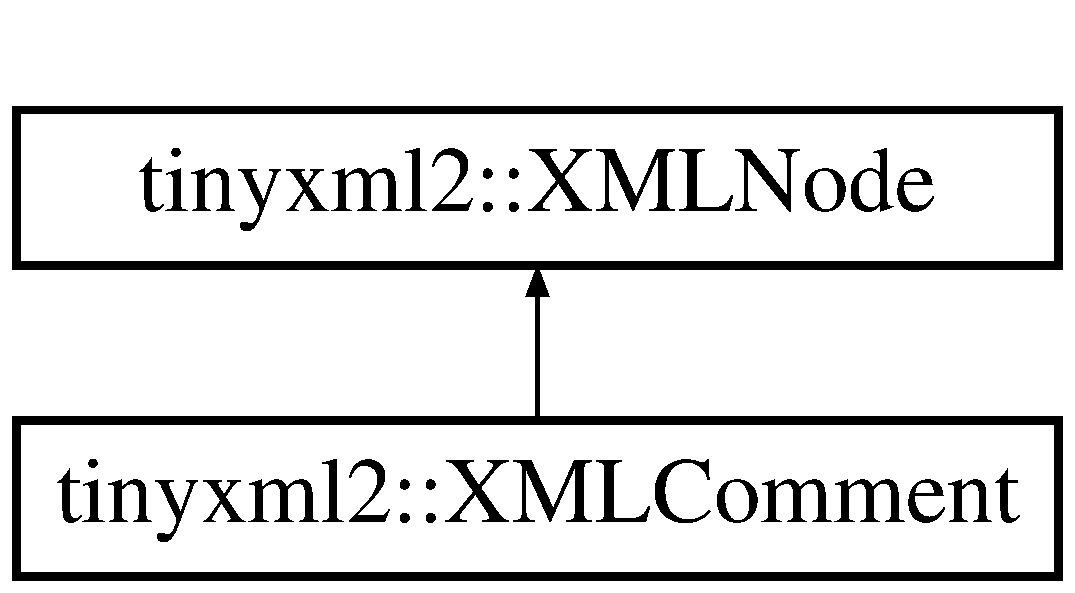
\includegraphics[height=2.000000cm]{classtinyxml2_1_1_x_m_l_comment}
\end{center}
\end{figure}
\subsection*{Public Member Functions}
\begin{DoxyCompactItemize}
\item 
virtual \textbf{ X\+M\+L\+Comment} $\ast$ \textbf{ To\+Comment} ()
\begin{DoxyCompactList}\small\item\em Safely cast to a Comment, or null. \end{DoxyCompactList}\item 
virtual const \textbf{ X\+M\+L\+Comment} $\ast$ \textbf{ To\+Comment} () const
\item 
virtual bool \textbf{ Accept} (\textbf{ X\+M\+L\+Visitor} $\ast$visitor) const
\item 
virtual \textbf{ X\+M\+L\+Node} $\ast$ \textbf{ Shallow\+Clone} (\textbf{ X\+M\+L\+Document} $\ast$document) const
\item 
virtual bool \textbf{ Shallow\+Equal} (const \textbf{ X\+M\+L\+Node} $\ast$compare) const
\end{DoxyCompactItemize}
\subsection*{Protected Member Functions}
\begin{DoxyCompactItemize}
\item 
\textbf{ X\+M\+L\+Comment} (\textbf{ X\+M\+L\+Document} $\ast$doc)
\item 
virtual \textbf{ $\sim$\+X\+M\+L\+Comment} ()
\item 
char $\ast$ \textbf{ Parse\+Deep} (char $\ast$p, \textbf{ Str\+Pair} $\ast$parent\+End\+Tag, int $\ast$cur\+Line\+Num\+Ptr)
\end{DoxyCompactItemize}
\subsection*{Private Member Functions}
\begin{DoxyCompactItemize}
\item 
\textbf{ X\+M\+L\+Comment} (const \textbf{ X\+M\+L\+Comment} \&)
\item 
\textbf{ X\+M\+L\+Comment} \& \textbf{ operator=} (const \textbf{ X\+M\+L\+Comment} \&)
\end{DoxyCompactItemize}
\subsection*{Friends}
\begin{DoxyCompactItemize}
\item 
class \textbf{ X\+M\+L\+Document}
\end{DoxyCompactItemize}
\subsection*{Additional Inherited Members}


\subsection{Detailed Description}
An X\+ML Comment. 

Definition at line 1024 of file tinyxml2.\+h.



\subsection{Constructor \& Destructor Documentation}
\mbox{\label{classtinyxml2_1_1_x_m_l_comment_ae6463adc3edd93a8e5a9b2b7e99cdf91}} 
\index{tinyxml2::XMLComment@{tinyxml2::XMLComment}!XMLComment@{XMLComment}}
\index{XMLComment@{XMLComment}!tinyxml2::XMLComment@{tinyxml2::XMLComment}}
\subsubsection{XMLComment()\hspace{0.1cm}{\footnotesize\ttfamily [1/2]}}
{\footnotesize\ttfamily tinyxml2\+::\+X\+M\+L\+Comment\+::\+X\+M\+L\+Comment (\begin{DoxyParamCaption}\item[{\textbf{ X\+M\+L\+Document} $\ast$}]{doc }\end{DoxyParamCaption})\hspace{0.3cm}{\ttfamily [explicit]}, {\ttfamily [protected]}}



Definition at line 1202 of file tinyxml2.\+cpp.

\mbox{\label{classtinyxml2_1_1_x_m_l_comment_ab592f69b47852455c1b32c5e31e453d0}} 
\index{tinyxml2::XMLComment@{tinyxml2::XMLComment}!````~XMLComment@{$\sim$XMLComment}}
\index{````~XMLComment@{$\sim$XMLComment}!tinyxml2::XMLComment@{tinyxml2::XMLComment}}
\subsubsection{$\sim$XMLComment()}
{\footnotesize\ttfamily tinyxml2\+::\+X\+M\+L\+Comment\+::$\sim$\+X\+M\+L\+Comment (\begin{DoxyParamCaption}{ }\end{DoxyParamCaption})\hspace{0.3cm}{\ttfamily [protected]}, {\ttfamily [virtual]}}



Definition at line 1207 of file tinyxml2.\+cpp.

\mbox{\label{classtinyxml2_1_1_x_m_l_comment_aa0a9aae0850ac0e70d3cd20f6cb44447}} 
\index{tinyxml2::XMLComment@{tinyxml2::XMLComment}!XMLComment@{XMLComment}}
\index{XMLComment@{XMLComment}!tinyxml2::XMLComment@{tinyxml2::XMLComment}}
\subsubsection{XMLComment()\hspace{0.1cm}{\footnotesize\ttfamily [2/2]}}
{\footnotesize\ttfamily tinyxml2\+::\+X\+M\+L\+Comment\+::\+X\+M\+L\+Comment (\begin{DoxyParamCaption}\item[{const \textbf{ X\+M\+L\+Comment} \&}]{ }\end{DoxyParamCaption})\hspace{0.3cm}{\ttfamily [private]}}



\subsection{Member Function Documentation}
\mbox{\label{classtinyxml2_1_1_x_m_l_comment_a27b37d16cea01b5329dfbbb4f9508e39}} 
\index{tinyxml2::XMLComment@{tinyxml2::XMLComment}!Accept@{Accept}}
\index{Accept@{Accept}!tinyxml2::XMLComment@{tinyxml2::XMLComment}}
\subsubsection{Accept()}
{\footnotesize\ttfamily bool tinyxml2\+::\+X\+M\+L\+Comment\+::\+Accept (\begin{DoxyParamCaption}\item[{\textbf{ X\+M\+L\+Visitor} $\ast$}]{visitor }\end{DoxyParamCaption}) const\hspace{0.3cm}{\ttfamily [virtual]}}

Accept a hierarchical visit of the nodes in the Tiny\+X\+M\+L-\/2 D\+OM. Every node in the X\+ML tree will be conditionally visited and the host will be called back via the \doxyref{X\+M\+L\+Visitor}{p.}{classtinyxml2_1_1_x_m_l_visitor} interface.

This is essentially a S\+AX interface for Tiny\+X\+M\+L-\/2. (Note however it doesn\textquotesingle{}t re-\/parse the X\+ML for the callbacks, so the performance of Tiny\+X\+M\+L-\/2 is unchanged by using this interface versus any other.)

The interface has been based on ideas from\+:


\begin{DoxyItemize}
\item {\texttt{ http\+://www.\+saxproject.\+org/}}
\item {\texttt{ http\+://c2.\+com/cgi/wiki?\+Hierarchical\+Visitor\+Pattern}}
\end{DoxyItemize}

Which are both good references for \char`\"{}visiting\char`\"{}.

An example of using \doxyref{Accept()}{p.}{classtinyxml2_1_1_x_m_l_comment_a27b37d16cea01b5329dfbbb4f9508e39}\+: \begin{DoxyVerb}XMLPrinter printer;
tinyxmlDoc.Accept( &printer );
const char* xmlcstr = printer.CStr();
\end{DoxyVerb}
 

Implements \textbf{ tinyxml2\+::\+X\+M\+L\+Node} \doxyref{}{p.}{classtinyxml2_1_1_x_m_l_node_a81e66df0a44c67a7af17f3b77a152785}.



Definition at line 1241 of file tinyxml2.\+cpp.



References T\+I\+X\+M\+L\+A\+S\+S\+E\+RT, and tinyxml2\+::\+X\+M\+L\+Visitor\+::\+Visit().

\mbox{\label{classtinyxml2_1_1_x_m_l_comment_ac8de55f8381d110740772e6bf6f5755a}} 
\index{tinyxml2::XMLComment@{tinyxml2::XMLComment}!operator=@{operator=}}
\index{operator=@{operator=}!tinyxml2::XMLComment@{tinyxml2::XMLComment}}
\subsubsection{operator=()}
{\footnotesize\ttfamily \textbf{ X\+M\+L\+Comment}\& tinyxml2\+::\+X\+M\+L\+Comment\+::operator= (\begin{DoxyParamCaption}\item[{const \textbf{ X\+M\+L\+Comment} \&}]{ }\end{DoxyParamCaption})\hspace{0.3cm}{\ttfamily [private]}}

\mbox{\label{classtinyxml2_1_1_x_m_l_comment_a3430281eed8d1023bafa9e633f44f509}} 
\index{tinyxml2::XMLComment@{tinyxml2::XMLComment}!ParseDeep@{ParseDeep}}
\index{ParseDeep@{ParseDeep}!tinyxml2::XMLComment@{tinyxml2::XMLComment}}
\subsubsection{ParseDeep()}
{\footnotesize\ttfamily char $\ast$ tinyxml2\+::\+X\+M\+L\+Comment\+::\+Parse\+Deep (\begin{DoxyParamCaption}\item[{char $\ast$}]{p,  }\item[{\textbf{ Str\+Pair} $\ast$}]{parent\+End\+Tag,  }\item[{int $\ast$}]{cur\+Line\+Num\+Ptr }\end{DoxyParamCaption})\hspace{0.3cm}{\ttfamily [protected]}, {\ttfamily [virtual]}}



Reimplemented from \textbf{ tinyxml2\+::\+X\+M\+L\+Node} \doxyref{}{p.}{classtinyxml2_1_1_x_m_l_node_a916e498914baecbc9a1f012352ef7c69}.



Definition at line 1212 of file tinyxml2.\+cpp.



References tinyxml2\+::\+X\+M\+L\+Node\+::\+\_\+document, tinyxml2\+::\+X\+M\+L\+Node\+::\+\_\+parse\+Line\+Num, tinyxml2\+::\+X\+M\+L\+Node\+::\+\_\+value, tinyxml2\+::\+Str\+Pair\+::\+C\+O\+M\+M\+E\+NT, tinyxml2\+::\+Str\+Pair\+::\+Parse\+Text(), tinyxml2\+::\+X\+M\+L\+Document\+::\+Set\+Error(), and tinyxml2\+::\+X\+M\+L\+\_\+\+E\+R\+R\+O\+R\+\_\+\+P\+A\+R\+S\+I\+N\+G\+\_\+\+C\+O\+M\+M\+E\+NT.

\mbox{\label{classtinyxml2_1_1_x_m_l_comment_adf5b5c0319351dcc339df098d11e8fb2}} 
\index{tinyxml2::XMLComment@{tinyxml2::XMLComment}!ShallowClone@{ShallowClone}}
\index{ShallowClone@{ShallowClone}!tinyxml2::XMLComment@{tinyxml2::XMLComment}}
\subsubsection{ShallowClone()}
{\footnotesize\ttfamily \textbf{ X\+M\+L\+Node} $\ast$ tinyxml2\+::\+X\+M\+L\+Comment\+::\+Shallow\+Clone (\begin{DoxyParamCaption}\item[{\textbf{ X\+M\+L\+Document} $\ast$}]{document }\end{DoxyParamCaption}) const\hspace{0.3cm}{\ttfamily [virtual]}}

Make a copy of this node, but not its children. You may pass in a Document pointer that will be the owner of the new Node. If the \textquotesingle{}document\textquotesingle{} is null, then the node returned will be allocated from the current Document. (this-\/$>$\doxyref{Get\+Document()}{p.}{classtinyxml2_1_1_x_m_l_node_af343d1ef0b45c0020e62d784d7e67a68})

Note\+: if called on a \doxyref{X\+M\+L\+Document}{p.}{classtinyxml2_1_1_x_m_l_document}, this will return null. 

Implements \textbf{ tinyxml2\+::\+X\+M\+L\+Node} \doxyref{}{p.}{classtinyxml2_1_1_x_m_l_node_a8402cbd3129d20e9e6024bbcc0531283}.



Definition at line 1223 of file tinyxml2.\+cpp.



References tinyxml2\+::\+X\+M\+L\+Node\+::\+\_\+document, tinyxml2\+::\+X\+M\+L\+Document\+::\+New\+Comment(), and tinyxml2\+::\+X\+M\+L\+Node\+::\+Value().

\mbox{\label{classtinyxml2_1_1_x_m_l_comment_a965d880a99d58dd915caa88dc37a9b51}} 
\index{tinyxml2::XMLComment@{tinyxml2::XMLComment}!ShallowEqual@{ShallowEqual}}
\index{ShallowEqual@{ShallowEqual}!tinyxml2::XMLComment@{tinyxml2::XMLComment}}
\subsubsection{ShallowEqual()}
{\footnotesize\ttfamily bool tinyxml2\+::\+X\+M\+L\+Comment\+::\+Shallow\+Equal (\begin{DoxyParamCaption}\item[{const \textbf{ X\+M\+L\+Node} $\ast$}]{compare }\end{DoxyParamCaption}) const\hspace{0.3cm}{\ttfamily [virtual]}}

Test if 2 nodes are the same, but don\textquotesingle{}t test children. The 2 nodes do not need to be in the same Document.

Note\+: if called on a \doxyref{X\+M\+L\+Document}{p.}{classtinyxml2_1_1_x_m_l_document}, this will return false. 

Implements \textbf{ tinyxml2\+::\+X\+M\+L\+Node} \doxyref{}{p.}{classtinyxml2_1_1_x_m_l_node_a7ce18b751c3ea09eac292dca264f9226}.



Definition at line 1233 of file tinyxml2.\+cpp.



References tinyxml2\+::\+X\+M\+L\+Util\+::\+String\+Equal(), T\+I\+X\+M\+L\+A\+S\+S\+E\+RT, tinyxml2\+::\+X\+M\+L\+Node\+::\+To\+Comment(), and tinyxml2\+::\+X\+M\+L\+Node\+::\+Value().

\mbox{\label{classtinyxml2_1_1_x_m_l_comment_a8093e1dc8a34fa446d9dc3fde0e6c0ee}} 
\index{tinyxml2::XMLComment@{tinyxml2::XMLComment}!ToComment@{ToComment}}
\index{ToComment@{ToComment}!tinyxml2::XMLComment@{tinyxml2::XMLComment}}
\subsubsection{ToComment()\hspace{0.1cm}{\footnotesize\ttfamily [1/2]}}
{\footnotesize\ttfamily virtual \textbf{ X\+M\+L\+Comment}$\ast$ tinyxml2\+::\+X\+M\+L\+Comment\+::\+To\+Comment (\begin{DoxyParamCaption}{ }\end{DoxyParamCaption})\hspace{0.3cm}{\ttfamily [inline]}, {\ttfamily [virtual]}}



Safely cast to a Comment, or null. 



Reimplemented from \textbf{ tinyxml2\+::\+X\+M\+L\+Node} \doxyref{}{p.}{classtinyxml2_1_1_x_m_l_node_aff47671055aa99840a1c1ebd661e63e3}.



Definition at line 1028 of file tinyxml2.\+h.

\mbox{\label{classtinyxml2_1_1_x_m_l_comment_a8e60caf06d8e88876a94b81db026b85c}} 
\index{tinyxml2::XMLComment@{tinyxml2::XMLComment}!ToComment@{ToComment}}
\index{ToComment@{ToComment}!tinyxml2::XMLComment@{tinyxml2::XMLComment}}
\subsubsection{ToComment()\hspace{0.1cm}{\footnotesize\ttfamily [2/2]}}
{\footnotesize\ttfamily virtual const \textbf{ X\+M\+L\+Comment}$\ast$ tinyxml2\+::\+X\+M\+L\+Comment\+::\+To\+Comment (\begin{DoxyParamCaption}{ }\end{DoxyParamCaption}) const\hspace{0.3cm}{\ttfamily [inline]}, {\ttfamily [virtual]}}



Reimplemented from \textbf{ tinyxml2\+::\+X\+M\+L\+Node} \doxyref{}{p.}{classtinyxml2_1_1_x_m_l_node_a6a53bb83faf5c0ccc95b6cf74dba0025}.



Definition at line 1031 of file tinyxml2.\+h.



\subsection{Friends And Related Function Documentation}
\mbox{\label{classtinyxml2_1_1_x_m_l_comment_a4eee3bda60c60a30e4e8cd4ea91c4c6e}} 
\index{tinyxml2::XMLComment@{tinyxml2::XMLComment}!XMLDocument@{XMLDocument}}
\index{XMLDocument@{XMLDocument}!tinyxml2::XMLComment@{tinyxml2::XMLComment}}
\subsubsection{XMLDocument}
{\footnotesize\ttfamily friend class \textbf{ X\+M\+L\+Document}\hspace{0.3cm}{\ttfamily [friend]}}



Definition at line 1026 of file tinyxml2.\+h.



The documentation for this class was generated from the following files\+:\begin{DoxyCompactItemize}
\item 
include/\textbf{ tinyxml2.\+h}\item 
src/\textbf{ tinyxml2.\+cpp}\end{DoxyCompactItemize}

\section{tinyxml2\+:\+:X\+M\+L\+Const\+Handle Class Reference}
\label{classtinyxml2_1_1_x_m_l_const_handle}\index{tinyxml2\+::\+X\+M\+L\+Const\+Handle@{tinyxml2\+::\+X\+M\+L\+Const\+Handle}}


{\ttfamily \#include $<$tinyxml2.\+h$>$}



Collaboration diagram for tinyxml2\+:\+:X\+M\+L\+Const\+Handle\+:
% FIG 0
\subsection*{Public Member Functions}
\begin{DoxyCompactItemize}
\item 
\textbf{ X\+M\+L\+Const\+Handle} (const \textbf{ X\+M\+L\+Node} $\ast$node)
\item 
\textbf{ X\+M\+L\+Const\+Handle} (const \textbf{ X\+M\+L\+Node} \&node)
\item 
\textbf{ X\+M\+L\+Const\+Handle} (const \textbf{ X\+M\+L\+Const\+Handle} \&ref)
\item 
\textbf{ X\+M\+L\+Const\+Handle} \& \textbf{ operator=} (const \textbf{ X\+M\+L\+Const\+Handle} \&ref)
\item 
const \textbf{ X\+M\+L\+Const\+Handle} \textbf{ First\+Child} () const
\item 
const \textbf{ X\+M\+L\+Const\+Handle} \textbf{ First\+Child\+Element} (const char $\ast$name=0) const
\item 
const \textbf{ X\+M\+L\+Const\+Handle} \textbf{ Last\+Child} () const
\item 
const \textbf{ X\+M\+L\+Const\+Handle} \textbf{ Last\+Child\+Element} (const char $\ast$name=0) const
\item 
const \textbf{ X\+M\+L\+Const\+Handle} \textbf{ Previous\+Sibling} () const
\item 
const \textbf{ X\+M\+L\+Const\+Handle} \textbf{ Previous\+Sibling\+Element} (const char $\ast$name=0) const
\item 
const \textbf{ X\+M\+L\+Const\+Handle} \textbf{ Next\+Sibling} () const
\item 
const \textbf{ X\+M\+L\+Const\+Handle} \textbf{ Next\+Sibling\+Element} (const char $\ast$name=0) const
\item 
const \textbf{ X\+M\+L\+Node} $\ast$ \textbf{ To\+Node} () const
\item 
const \textbf{ X\+M\+L\+Element} $\ast$ \textbf{ To\+Element} () const
\item 
const \textbf{ X\+M\+L\+Text} $\ast$ \textbf{ To\+Text} () const
\item 
const \textbf{ X\+M\+L\+Unknown} $\ast$ \textbf{ To\+Unknown} () const
\item 
const \textbf{ X\+M\+L\+Declaration} $\ast$ \textbf{ To\+Declaration} () const
\end{DoxyCompactItemize}
\subsection*{Private Attributes}
\begin{DoxyCompactItemize}
\item 
const \textbf{ X\+M\+L\+Node} $\ast$ \textbf{ \+\_\+node}
\end{DoxyCompactItemize}


\subsection{Detailed Description}
A variant of the \doxyref{X\+M\+L\+Handle}{p.}{classtinyxml2_1_1_x_m_l_handle} class for working with const X\+M\+L\+Nodes and Documents. It is the same in all regards, except for the \textquotesingle{}const\textquotesingle{} qualifiers. See \doxyref{X\+M\+L\+Handle}{p.}{classtinyxml2_1_1_x_m_l_handle} for A\+PI. 

Definition at line 2071 of file tinyxml2.\+h.



\subsection{Constructor \& Destructor Documentation}
\mbox{\label{classtinyxml2_1_1_x_m_l_const_handle_a098bda71fa11d7c74ccddab59d5dd534}} 
\index{tinyxml2\+::\+X\+M\+L\+Const\+Handle@{tinyxml2\+::\+X\+M\+L\+Const\+Handle}!X\+M\+L\+Const\+Handle@{X\+M\+L\+Const\+Handle}}
\index{X\+M\+L\+Const\+Handle@{X\+M\+L\+Const\+Handle}!tinyxml2\+::\+X\+M\+L\+Const\+Handle@{tinyxml2\+::\+X\+M\+L\+Const\+Handle}}
\subsubsection{X\+M\+L\+Const\+Handle()\hspace{0.1cm}{\footnotesize\ttfamily [1/3]}}
{\footnotesize\ttfamily tinyxml2\+::\+X\+M\+L\+Const\+Handle\+::\+X\+M\+L\+Const\+Handle (\begin{DoxyParamCaption}\item[{const \textbf{ X\+M\+L\+Node} $\ast$}]{node }\end{DoxyParamCaption})\hspace{0.3cm}{\ttfamily [inline]}, {\ttfamily [explicit]}}



Definition at line 2074 of file tinyxml2.\+h.

\mbox{\label{classtinyxml2_1_1_x_m_l_const_handle_a8420a0c4720637e0529e78c2e22f2b0b}} 
\index{tinyxml2\+::\+X\+M\+L\+Const\+Handle@{tinyxml2\+::\+X\+M\+L\+Const\+Handle}!X\+M\+L\+Const\+Handle@{X\+M\+L\+Const\+Handle}}
\index{X\+M\+L\+Const\+Handle@{X\+M\+L\+Const\+Handle}!tinyxml2\+::\+X\+M\+L\+Const\+Handle@{tinyxml2\+::\+X\+M\+L\+Const\+Handle}}
\subsubsection{X\+M\+L\+Const\+Handle()\hspace{0.1cm}{\footnotesize\ttfamily [2/3]}}
{\footnotesize\ttfamily tinyxml2\+::\+X\+M\+L\+Const\+Handle\+::\+X\+M\+L\+Const\+Handle (\begin{DoxyParamCaption}\item[{const \textbf{ X\+M\+L\+Node} \&}]{node }\end{DoxyParamCaption})\hspace{0.3cm}{\ttfamily [inline]}, {\ttfamily [explicit]}}



Definition at line 2076 of file tinyxml2.\+h.

\mbox{\label{classtinyxml2_1_1_x_m_l_const_handle_a639317ad315ff24f4ef0dc69312d7303}} 
\index{tinyxml2\+::\+X\+M\+L\+Const\+Handle@{tinyxml2\+::\+X\+M\+L\+Const\+Handle}!X\+M\+L\+Const\+Handle@{X\+M\+L\+Const\+Handle}}
\index{X\+M\+L\+Const\+Handle@{X\+M\+L\+Const\+Handle}!tinyxml2\+::\+X\+M\+L\+Const\+Handle@{tinyxml2\+::\+X\+M\+L\+Const\+Handle}}
\subsubsection{X\+M\+L\+Const\+Handle()\hspace{0.1cm}{\footnotesize\ttfamily [3/3]}}
{\footnotesize\ttfamily tinyxml2\+::\+X\+M\+L\+Const\+Handle\+::\+X\+M\+L\+Const\+Handle (\begin{DoxyParamCaption}\item[{const \textbf{ X\+M\+L\+Const\+Handle} \&}]{ref }\end{DoxyParamCaption})\hspace{0.3cm}{\ttfamily [inline]}}



Definition at line 2078 of file tinyxml2.\+h.



\subsection{Member Function Documentation}
\mbox{\label{classtinyxml2_1_1_x_m_l_const_handle_aef06bd16cb308652a32b864b0a743136}} 
\index{tinyxml2\+::\+X\+M\+L\+Const\+Handle@{tinyxml2\+::\+X\+M\+L\+Const\+Handle}!First\+Child@{First\+Child}}
\index{First\+Child@{First\+Child}!tinyxml2\+::\+X\+M\+L\+Const\+Handle@{tinyxml2\+::\+X\+M\+L\+Const\+Handle}}
\subsubsection{First\+Child()}
{\footnotesize\ttfamily const \textbf{ X\+M\+L\+Const\+Handle} tinyxml2\+::\+X\+M\+L\+Const\+Handle\+::\+First\+Child (\begin{DoxyParamCaption}{ }\end{DoxyParamCaption}) const\hspace{0.3cm}{\ttfamily [inline]}}



Definition at line 2086 of file tinyxml2.\+h.

\mbox{\label{classtinyxml2_1_1_x_m_l_const_handle_ac747db472ffc55c5af2e82ffec813640}} 
\index{tinyxml2\+::\+X\+M\+L\+Const\+Handle@{tinyxml2\+::\+X\+M\+L\+Const\+Handle}!First\+Child\+Element@{First\+Child\+Element}}
\index{First\+Child\+Element@{First\+Child\+Element}!tinyxml2\+::\+X\+M\+L\+Const\+Handle@{tinyxml2\+::\+X\+M\+L\+Const\+Handle}}
\subsubsection{First\+Child\+Element()}
{\footnotesize\ttfamily const \textbf{ X\+M\+L\+Const\+Handle} tinyxml2\+::\+X\+M\+L\+Const\+Handle\+::\+First\+Child\+Element (\begin{DoxyParamCaption}\item[{const char $\ast$}]{name = {\ttfamily 0} }\end{DoxyParamCaption}) const\hspace{0.3cm}{\ttfamily [inline]}}



Definition at line 2089 of file tinyxml2.\+h.

\mbox{\label{classtinyxml2_1_1_x_m_l_const_handle_a908436124990f3d7b35cb7df20d31d9e}} 
\index{tinyxml2\+::\+X\+M\+L\+Const\+Handle@{tinyxml2\+::\+X\+M\+L\+Const\+Handle}!Last\+Child@{Last\+Child}}
\index{Last\+Child@{Last\+Child}!tinyxml2\+::\+X\+M\+L\+Const\+Handle@{tinyxml2\+::\+X\+M\+L\+Const\+Handle}}
\subsubsection{Last\+Child()}
{\footnotesize\ttfamily const \textbf{ X\+M\+L\+Const\+Handle} tinyxml2\+::\+X\+M\+L\+Const\+Handle\+::\+Last\+Child (\begin{DoxyParamCaption}{ }\end{DoxyParamCaption}) const\hspace{0.3cm}{\ttfamily [inline]}}



Definition at line 2092 of file tinyxml2.\+h.

\mbox{\label{classtinyxml2_1_1_x_m_l_const_handle_a9de0475ec42bd50c0e64624a250ba5b2}} 
\index{tinyxml2\+::\+X\+M\+L\+Const\+Handle@{tinyxml2\+::\+X\+M\+L\+Const\+Handle}!Last\+Child\+Element@{Last\+Child\+Element}}
\index{Last\+Child\+Element@{Last\+Child\+Element}!tinyxml2\+::\+X\+M\+L\+Const\+Handle@{tinyxml2\+::\+X\+M\+L\+Const\+Handle}}
\subsubsection{Last\+Child\+Element()}
{\footnotesize\ttfamily const \textbf{ X\+M\+L\+Const\+Handle} tinyxml2\+::\+X\+M\+L\+Const\+Handle\+::\+Last\+Child\+Element (\begin{DoxyParamCaption}\item[{const char $\ast$}]{name = {\ttfamily 0} }\end{DoxyParamCaption}) const\hspace{0.3cm}{\ttfamily [inline]}}



Definition at line 2095 of file tinyxml2.\+h.

\mbox{\label{classtinyxml2_1_1_x_m_l_const_handle_aec3710e455f41014026ef17fbbb0efb3}} 
\index{tinyxml2\+::\+X\+M\+L\+Const\+Handle@{tinyxml2\+::\+X\+M\+L\+Const\+Handle}!Next\+Sibling@{Next\+Sibling}}
\index{Next\+Sibling@{Next\+Sibling}!tinyxml2\+::\+X\+M\+L\+Const\+Handle@{tinyxml2\+::\+X\+M\+L\+Const\+Handle}}
\subsubsection{Next\+Sibling()}
{\footnotesize\ttfamily const \textbf{ X\+M\+L\+Const\+Handle} tinyxml2\+::\+X\+M\+L\+Const\+Handle\+::\+Next\+Sibling (\begin{DoxyParamCaption}{ }\end{DoxyParamCaption}) const\hspace{0.3cm}{\ttfamily [inline]}}



Definition at line 2104 of file tinyxml2.\+h.

\mbox{\label{classtinyxml2_1_1_x_m_l_const_handle_a3c9e6b48b02d3d5232e1e8780753d8a5}} 
\index{tinyxml2\+::\+X\+M\+L\+Const\+Handle@{tinyxml2\+::\+X\+M\+L\+Const\+Handle}!Next\+Sibling\+Element@{Next\+Sibling\+Element}}
\index{Next\+Sibling\+Element@{Next\+Sibling\+Element}!tinyxml2\+::\+X\+M\+L\+Const\+Handle@{tinyxml2\+::\+X\+M\+L\+Const\+Handle}}
\subsubsection{Next\+Sibling\+Element()}
{\footnotesize\ttfamily const \textbf{ X\+M\+L\+Const\+Handle} tinyxml2\+::\+X\+M\+L\+Const\+Handle\+::\+Next\+Sibling\+Element (\begin{DoxyParamCaption}\item[{const char $\ast$}]{name = {\ttfamily 0} }\end{DoxyParamCaption}) const\hspace{0.3cm}{\ttfamily [inline]}}



Definition at line 2107 of file tinyxml2.\+h.

\mbox{\label{classtinyxml2_1_1_x_m_l_const_handle_a2d74c91df1ff9aa5f9b57e3dceddbf94}} 
\index{tinyxml2\+::\+X\+M\+L\+Const\+Handle@{tinyxml2\+::\+X\+M\+L\+Const\+Handle}!operator=@{operator=}}
\index{operator=@{operator=}!tinyxml2\+::\+X\+M\+L\+Const\+Handle@{tinyxml2\+::\+X\+M\+L\+Const\+Handle}}
\subsubsection{operator=()}
{\footnotesize\ttfamily \textbf{ X\+M\+L\+Const\+Handle}\& tinyxml2\+::\+X\+M\+L\+Const\+Handle\+::operator= (\begin{DoxyParamCaption}\item[{const \textbf{ X\+M\+L\+Const\+Handle} \&}]{ref }\end{DoxyParamCaption})\hspace{0.3cm}{\ttfamily [inline]}}



Definition at line 2081 of file tinyxml2.\+h.



References \+\_\+node.

\mbox{\label{classtinyxml2_1_1_x_m_l_const_handle_acf68cc7930e4ac883e0c7e16ef2fbb66}} 
\index{tinyxml2\+::\+X\+M\+L\+Const\+Handle@{tinyxml2\+::\+X\+M\+L\+Const\+Handle}!Previous\+Sibling@{Previous\+Sibling}}
\index{Previous\+Sibling@{Previous\+Sibling}!tinyxml2\+::\+X\+M\+L\+Const\+Handle@{tinyxml2\+::\+X\+M\+L\+Const\+Handle}}
\subsubsection{Previous\+Sibling()}
{\footnotesize\ttfamily const \textbf{ X\+M\+L\+Const\+Handle} tinyxml2\+::\+X\+M\+L\+Const\+Handle\+::\+Previous\+Sibling (\begin{DoxyParamCaption}{ }\end{DoxyParamCaption}) const\hspace{0.3cm}{\ttfamily [inline]}}



Definition at line 2098 of file tinyxml2.\+h.

\mbox{\label{classtinyxml2_1_1_x_m_l_const_handle_aef99308659f2617299ac29980769a91e}} 
\index{tinyxml2\+::\+X\+M\+L\+Const\+Handle@{tinyxml2\+::\+X\+M\+L\+Const\+Handle}!Previous\+Sibling\+Element@{Previous\+Sibling\+Element}}
\index{Previous\+Sibling\+Element@{Previous\+Sibling\+Element}!tinyxml2\+::\+X\+M\+L\+Const\+Handle@{tinyxml2\+::\+X\+M\+L\+Const\+Handle}}
\subsubsection{Previous\+Sibling\+Element()}
{\footnotesize\ttfamily const \textbf{ X\+M\+L\+Const\+Handle} tinyxml2\+::\+X\+M\+L\+Const\+Handle\+::\+Previous\+Sibling\+Element (\begin{DoxyParamCaption}\item[{const char $\ast$}]{name = {\ttfamily 0} }\end{DoxyParamCaption}) const\hspace{0.3cm}{\ttfamily [inline]}}



Definition at line 2101 of file tinyxml2.\+h.

\mbox{\label{classtinyxml2_1_1_x_m_l_const_handle_a55e306d105fa80d626041e4d3b77b716}} 
\index{tinyxml2\+::\+X\+M\+L\+Const\+Handle@{tinyxml2\+::\+X\+M\+L\+Const\+Handle}!To\+Declaration@{To\+Declaration}}
\index{To\+Declaration@{To\+Declaration}!tinyxml2\+::\+X\+M\+L\+Const\+Handle@{tinyxml2\+::\+X\+M\+L\+Const\+Handle}}
\subsubsection{To\+Declaration()}
{\footnotesize\ttfamily const \textbf{ X\+M\+L\+Declaration}$\ast$ tinyxml2\+::\+X\+M\+L\+Const\+Handle\+::\+To\+Declaration (\begin{DoxyParamCaption}{ }\end{DoxyParamCaption}) const\hspace{0.3cm}{\ttfamily [inline]}}



Definition at line 2124 of file tinyxml2.\+h.

\mbox{\label{classtinyxml2_1_1_x_m_l_const_handle_a4dba53c6e201d412e915620feaaa56f3}} 
\index{tinyxml2\+::\+X\+M\+L\+Const\+Handle@{tinyxml2\+::\+X\+M\+L\+Const\+Handle}!To\+Element@{To\+Element}}
\index{To\+Element@{To\+Element}!tinyxml2\+::\+X\+M\+L\+Const\+Handle@{tinyxml2\+::\+X\+M\+L\+Const\+Handle}}
\subsubsection{To\+Element()}
{\footnotesize\ttfamily const \textbf{ X\+M\+L\+Element}$\ast$ tinyxml2\+::\+X\+M\+L\+Const\+Handle\+::\+To\+Element (\begin{DoxyParamCaption}{ }\end{DoxyParamCaption}) const\hspace{0.3cm}{\ttfamily [inline]}}



Definition at line 2115 of file tinyxml2.\+h.

\mbox{\label{classtinyxml2_1_1_x_m_l_const_handle_a61812760cb08bc1b050e65b73a08457b}} 
\index{tinyxml2\+::\+X\+M\+L\+Const\+Handle@{tinyxml2\+::\+X\+M\+L\+Const\+Handle}!To\+Node@{To\+Node}}
\index{To\+Node@{To\+Node}!tinyxml2\+::\+X\+M\+L\+Const\+Handle@{tinyxml2\+::\+X\+M\+L\+Const\+Handle}}
\subsubsection{To\+Node()}
{\footnotesize\ttfamily const \textbf{ X\+M\+L\+Node}$\ast$ tinyxml2\+::\+X\+M\+L\+Const\+Handle\+::\+To\+Node (\begin{DoxyParamCaption}{ }\end{DoxyParamCaption}) const\hspace{0.3cm}{\ttfamily [inline]}}



Definition at line 2112 of file tinyxml2.\+h.

\mbox{\label{classtinyxml2_1_1_x_m_l_const_handle_a80e24d90d476005aa35602a665358e2d}} 
\index{tinyxml2\+::\+X\+M\+L\+Const\+Handle@{tinyxml2\+::\+X\+M\+L\+Const\+Handle}!To\+Text@{To\+Text}}
\index{To\+Text@{To\+Text}!tinyxml2\+::\+X\+M\+L\+Const\+Handle@{tinyxml2\+::\+X\+M\+L\+Const\+Handle}}
\subsubsection{To\+Text()}
{\footnotesize\ttfamily const \textbf{ X\+M\+L\+Text}$\ast$ tinyxml2\+::\+X\+M\+L\+Const\+Handle\+::\+To\+Text (\begin{DoxyParamCaption}{ }\end{DoxyParamCaption}) const\hspace{0.3cm}{\ttfamily [inline]}}



Definition at line 2118 of file tinyxml2.\+h.

\mbox{\label{classtinyxml2_1_1_x_m_l_const_handle_a4395e5feaba7b456a81ca274880ea3d3}} 
\index{tinyxml2\+::\+X\+M\+L\+Const\+Handle@{tinyxml2\+::\+X\+M\+L\+Const\+Handle}!To\+Unknown@{To\+Unknown}}
\index{To\+Unknown@{To\+Unknown}!tinyxml2\+::\+X\+M\+L\+Const\+Handle@{tinyxml2\+::\+X\+M\+L\+Const\+Handle}}
\subsubsection{To\+Unknown()}
{\footnotesize\ttfamily const \textbf{ X\+M\+L\+Unknown}$\ast$ tinyxml2\+::\+X\+M\+L\+Const\+Handle\+::\+To\+Unknown (\begin{DoxyParamCaption}{ }\end{DoxyParamCaption}) const\hspace{0.3cm}{\ttfamily [inline]}}



Definition at line 2121 of file tinyxml2.\+h.



\subsection{Member Data Documentation}
\mbox{\label{classtinyxml2_1_1_x_m_l_const_handle_ad4d8db839660ef730adfa2439945c4da}} 
\index{tinyxml2\+::\+X\+M\+L\+Const\+Handle@{tinyxml2\+::\+X\+M\+L\+Const\+Handle}!\+\_\+node@{\+\_\+node}}
\index{\+\_\+node@{\+\_\+node}!tinyxml2\+::\+X\+M\+L\+Const\+Handle@{tinyxml2\+::\+X\+M\+L\+Const\+Handle}}
\subsubsection{\+\_\+node}
{\footnotesize\ttfamily const \textbf{ X\+M\+L\+Node}$\ast$ tinyxml2\+::\+X\+M\+L\+Const\+Handle\+::\+\_\+node\hspace{0.3cm}{\ttfamily [private]}}



Definition at line 2129 of file tinyxml2.\+h.



Referenced by operator=().



The documentation for this class was generated from the following file\+:\begin{DoxyCompactItemize}
\item 
include/\textbf{ tinyxml2.\+h}\end{DoxyCompactItemize}

\section{tinyxml2\+::X\+M\+L\+Declaration Class Reference}
\label{classtinyxml2_1_1_x_m_l_declaration}\index{tinyxml2::XMLDeclaration@{tinyxml2::XMLDeclaration}}


{\ttfamily \#include $<$tinyxml2.\+h$>$}

Inheritance diagram for tinyxml2\+::X\+M\+L\+Declaration\+:\begin{figure}[H]
\begin{center}
\leavevmode
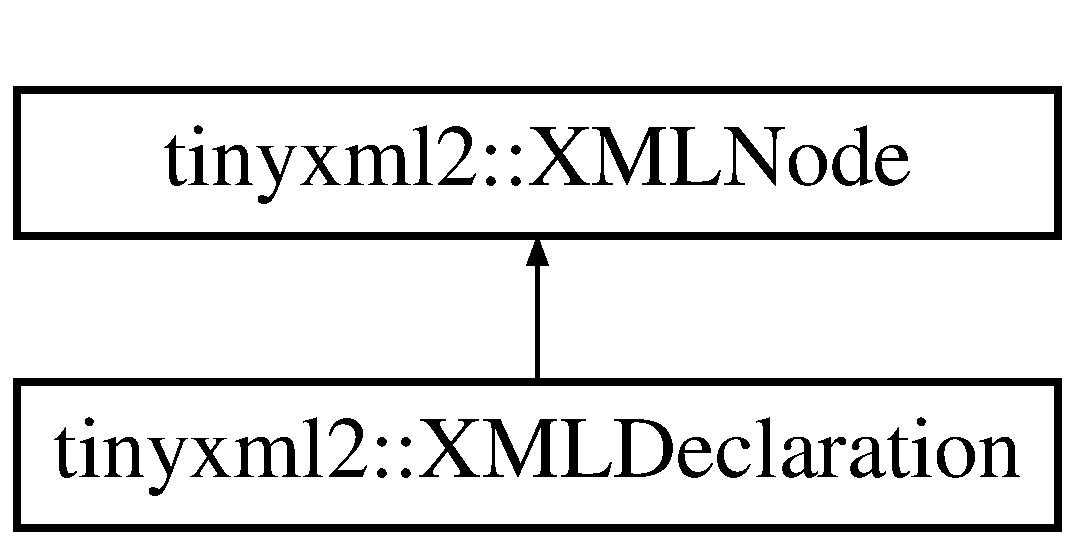
\includegraphics[height=2.000000cm]{classtinyxml2_1_1_x_m_l_declaration}
\end{center}
\end{figure}
\subsection*{Public Member Functions}
\begin{DoxyCompactItemize}
\item 
virtual \textbf{ X\+M\+L\+Declaration} $\ast$ \textbf{ To\+Declaration} ()
\begin{DoxyCompactList}\small\item\em Safely cast to a Declaration, or null. \end{DoxyCompactList}\item 
virtual const \textbf{ X\+M\+L\+Declaration} $\ast$ \textbf{ To\+Declaration} () const
\item 
virtual bool \textbf{ Accept} (\textbf{ X\+M\+L\+Visitor} $\ast$visitor) const
\item 
virtual \textbf{ X\+M\+L\+Node} $\ast$ \textbf{ Shallow\+Clone} (\textbf{ X\+M\+L\+Document} $\ast$document) const
\item 
virtual bool \textbf{ Shallow\+Equal} (const \textbf{ X\+M\+L\+Node} $\ast$compare) const
\end{DoxyCompactItemize}
\subsection*{Protected Member Functions}
\begin{DoxyCompactItemize}
\item 
\textbf{ X\+M\+L\+Declaration} (\textbf{ X\+M\+L\+Document} $\ast$doc)
\item 
virtual \textbf{ $\sim$\+X\+M\+L\+Declaration} ()
\item 
char $\ast$ \textbf{ Parse\+Deep} (char $\ast$p, \textbf{ Str\+Pair} $\ast$parent\+End\+Tag, int $\ast$cur\+Line\+Num\+Ptr)
\end{DoxyCompactItemize}
\subsection*{Private Member Functions}
\begin{DoxyCompactItemize}
\item 
\textbf{ X\+M\+L\+Declaration} (const \textbf{ X\+M\+L\+Declaration} \&)
\item 
\textbf{ X\+M\+L\+Declaration} \& \textbf{ operator=} (const \textbf{ X\+M\+L\+Declaration} \&)
\end{DoxyCompactItemize}
\subsection*{Friends}
\begin{DoxyCompactItemize}
\item 
class \textbf{ X\+M\+L\+Document}
\end{DoxyCompactItemize}
\subsection*{Additional Inherited Members}


\subsection{Detailed Description}
In correct X\+ML the declaration is the first entry in the file. \begin{DoxyVerb}    <?xml version="1.0" standalone="yes"?>
\end{DoxyVerb}


Tiny\+X\+M\+L-\/2 will happily read or write files without a declaration, however.

The text of the declaration isn\textquotesingle{}t interpreted. It is parsed and written as a string. 

Definition at line 1063 of file tinyxml2.\+h.



\subsection{Constructor \& Destructor Documentation}
\mbox{\label{classtinyxml2_1_1_x_m_l_declaration_aef9586f2ce5df5feba74dde49a242b06}} 
\index{tinyxml2::XMLDeclaration@{tinyxml2::XMLDeclaration}!XMLDeclaration@{XMLDeclaration}}
\index{XMLDeclaration@{XMLDeclaration}!tinyxml2::XMLDeclaration@{tinyxml2::XMLDeclaration}}
\subsubsection{XMLDeclaration()\hspace{0.1cm}{\footnotesize\ttfamily [1/2]}}
{\footnotesize\ttfamily tinyxml2\+::\+X\+M\+L\+Declaration\+::\+X\+M\+L\+Declaration (\begin{DoxyParamCaption}\item[{\textbf{ X\+M\+L\+Document} $\ast$}]{doc }\end{DoxyParamCaption})\hspace{0.3cm}{\ttfamily [explicit]}, {\ttfamily [protected]}}



Definition at line 1250 of file tinyxml2.\+cpp.

\mbox{\label{classtinyxml2_1_1_x_m_l_declaration_ab93d5bf4f5d58b4144963cf739cf6dcc}} 
\index{tinyxml2::XMLDeclaration@{tinyxml2::XMLDeclaration}!````~XMLDeclaration@{$\sim$XMLDeclaration}}
\index{````~XMLDeclaration@{$\sim$XMLDeclaration}!tinyxml2::XMLDeclaration@{tinyxml2::XMLDeclaration}}
\subsubsection{$\sim$XMLDeclaration()}
{\footnotesize\ttfamily tinyxml2\+::\+X\+M\+L\+Declaration\+::$\sim$\+X\+M\+L\+Declaration (\begin{DoxyParamCaption}{ }\end{DoxyParamCaption})\hspace{0.3cm}{\ttfamily [protected]}, {\ttfamily [virtual]}}



Definition at line 1255 of file tinyxml2.\+cpp.

\mbox{\label{classtinyxml2_1_1_x_m_l_declaration_a5229cc0b31f034f93289af27ec3e2836}} 
\index{tinyxml2::XMLDeclaration@{tinyxml2::XMLDeclaration}!XMLDeclaration@{XMLDeclaration}}
\index{XMLDeclaration@{XMLDeclaration}!tinyxml2::XMLDeclaration@{tinyxml2::XMLDeclaration}}
\subsubsection{XMLDeclaration()\hspace{0.1cm}{\footnotesize\ttfamily [2/2]}}
{\footnotesize\ttfamily tinyxml2\+::\+X\+M\+L\+Declaration\+::\+X\+M\+L\+Declaration (\begin{DoxyParamCaption}\item[{const \textbf{ X\+M\+L\+Declaration} \&}]{ }\end{DoxyParamCaption})\hspace{0.3cm}{\ttfamily [private]}}



\subsection{Member Function Documentation}
\mbox{\label{classtinyxml2_1_1_x_m_l_declaration_acf47629d9fc08ed6f1c164a97bcf794b}} 
\index{tinyxml2::XMLDeclaration@{tinyxml2::XMLDeclaration}!Accept@{Accept}}
\index{Accept@{Accept}!tinyxml2::XMLDeclaration@{tinyxml2::XMLDeclaration}}
\subsubsection{Accept()}
{\footnotesize\ttfamily bool tinyxml2\+::\+X\+M\+L\+Declaration\+::\+Accept (\begin{DoxyParamCaption}\item[{\textbf{ X\+M\+L\+Visitor} $\ast$}]{visitor }\end{DoxyParamCaption}) const\hspace{0.3cm}{\ttfamily [virtual]}}

Accept a hierarchical visit of the nodes in the Tiny\+X\+M\+L-\/2 D\+OM. Every node in the X\+ML tree will be conditionally visited and the host will be called back via the \doxyref{X\+M\+L\+Visitor}{p.}{classtinyxml2_1_1_x_m_l_visitor} interface.

This is essentially a S\+AX interface for Tiny\+X\+M\+L-\/2. (Note however it doesn\textquotesingle{}t re-\/parse the X\+ML for the callbacks, so the performance of Tiny\+X\+M\+L-\/2 is unchanged by using this interface versus any other.)

The interface has been based on ideas from\+:


\begin{DoxyItemize}
\item {\texttt{ http\+://www.\+saxproject.\+org/}}
\item {\texttt{ http\+://c2.\+com/cgi/wiki?\+Hierarchical\+Visitor\+Pattern}}
\end{DoxyItemize}

Which are both good references for \char`\"{}visiting\char`\"{}.

An example of using \doxyref{Accept()}{p.}{classtinyxml2_1_1_x_m_l_declaration_acf47629d9fc08ed6f1c164a97bcf794b}\+: \begin{DoxyVerb}XMLPrinter printer;
tinyxmlDoc.Accept( &printer );
const char* xmlcstr = printer.CStr();
\end{DoxyVerb}
 

Implements \textbf{ tinyxml2\+::\+X\+M\+L\+Node} \doxyref{}{p.}{classtinyxml2_1_1_x_m_l_node_a81e66df0a44c67a7af17f3b77a152785}.



Definition at line 1291 of file tinyxml2.\+cpp.



References T\+I\+X\+M\+L\+A\+S\+S\+E\+RT, and tinyxml2\+::\+X\+M\+L\+Visitor\+::\+Visit().

\mbox{\label{classtinyxml2_1_1_x_m_l_declaration_a79eb518c2c2b1b99a122a5d5a308b7ee}} 
\index{tinyxml2::XMLDeclaration@{tinyxml2::XMLDeclaration}!operator=@{operator=}}
\index{operator=@{operator=}!tinyxml2::XMLDeclaration@{tinyxml2::XMLDeclaration}}
\subsubsection{operator=()}
{\footnotesize\ttfamily \textbf{ X\+M\+L\+Declaration}\& tinyxml2\+::\+X\+M\+L\+Declaration\+::operator= (\begin{DoxyParamCaption}\item[{const \textbf{ X\+M\+L\+Declaration} \&}]{ }\end{DoxyParamCaption})\hspace{0.3cm}{\ttfamily [private]}}

\mbox{\label{classtinyxml2_1_1_x_m_l_declaration_a42a2a36f4d78dc745063b79c16538b9b}} 
\index{tinyxml2::XMLDeclaration@{tinyxml2::XMLDeclaration}!ParseDeep@{ParseDeep}}
\index{ParseDeep@{ParseDeep}!tinyxml2::XMLDeclaration@{tinyxml2::XMLDeclaration}}
\subsubsection{ParseDeep()}
{\footnotesize\ttfamily char $\ast$ tinyxml2\+::\+X\+M\+L\+Declaration\+::\+Parse\+Deep (\begin{DoxyParamCaption}\item[{char $\ast$}]{p,  }\item[{\textbf{ Str\+Pair} $\ast$}]{parent\+End\+Tag,  }\item[{int $\ast$}]{cur\+Line\+Num\+Ptr }\end{DoxyParamCaption})\hspace{0.3cm}{\ttfamily [protected]}, {\ttfamily [virtual]}}



Reimplemented from \textbf{ tinyxml2\+::\+X\+M\+L\+Node} \doxyref{}{p.}{classtinyxml2_1_1_x_m_l_node_a916e498914baecbc9a1f012352ef7c69}.



Definition at line 1261 of file tinyxml2.\+cpp.



References tinyxml2\+::\+X\+M\+L\+Node\+::\+\_\+document, tinyxml2\+::\+X\+M\+L\+Node\+::\+\_\+parse\+Line\+Num, tinyxml2\+::\+X\+M\+L\+Node\+::\+\_\+value, tinyxml2\+::\+Str\+Pair\+::\+N\+E\+E\+D\+S\+\_\+\+N\+E\+W\+L\+I\+N\+E\+\_\+\+N\+O\+R\+M\+A\+L\+I\+Z\+A\+T\+I\+ON, tinyxml2\+::\+Str\+Pair\+::\+Parse\+Text(), tinyxml2\+::\+X\+M\+L\+Document\+::\+Set\+Error(), and tinyxml2\+::\+X\+M\+L\+\_\+\+E\+R\+R\+O\+R\+\_\+\+P\+A\+R\+S\+I\+N\+G\+\_\+\+D\+E\+C\+L\+A\+R\+A\+T\+I\+ON.

\mbox{\label{classtinyxml2_1_1_x_m_l_declaration_ad9d60e6d2df75c13eb6bf7319985b747}} 
\index{tinyxml2::XMLDeclaration@{tinyxml2::XMLDeclaration}!ShallowClone@{ShallowClone}}
\index{ShallowClone@{ShallowClone}!tinyxml2::XMLDeclaration@{tinyxml2::XMLDeclaration}}
\subsubsection{ShallowClone()}
{\footnotesize\ttfamily \textbf{ X\+M\+L\+Node} $\ast$ tinyxml2\+::\+X\+M\+L\+Declaration\+::\+Shallow\+Clone (\begin{DoxyParamCaption}\item[{\textbf{ X\+M\+L\+Document} $\ast$}]{document }\end{DoxyParamCaption}) const\hspace{0.3cm}{\ttfamily [virtual]}}

Make a copy of this node, but not its children. You may pass in a Document pointer that will be the owner of the new Node. If the \textquotesingle{}document\textquotesingle{} is null, then the node returned will be allocated from the current Document. (this-\/$>$\doxyref{Get\+Document()}{p.}{classtinyxml2_1_1_x_m_l_node_af343d1ef0b45c0020e62d784d7e67a68})

Note\+: if called on a \doxyref{X\+M\+L\+Document}{p.}{classtinyxml2_1_1_x_m_l_document}, this will return null. 

Implements \textbf{ tinyxml2\+::\+X\+M\+L\+Node} \doxyref{}{p.}{classtinyxml2_1_1_x_m_l_node_a8402cbd3129d20e9e6024bbcc0531283}.



Definition at line 1272 of file tinyxml2.\+cpp.



References tinyxml2\+::\+X\+M\+L\+Node\+::\+\_\+document, tinyxml2\+::\+X\+M\+L\+Document\+::\+New\+Declaration(), and tinyxml2\+::\+X\+M\+L\+Node\+::\+Value().

\mbox{\label{classtinyxml2_1_1_x_m_l_declaration_ae8b4d3a399857029f36c322b0801b69c}} 
\index{tinyxml2::XMLDeclaration@{tinyxml2::XMLDeclaration}!ShallowEqual@{ShallowEqual}}
\index{ShallowEqual@{ShallowEqual}!tinyxml2::XMLDeclaration@{tinyxml2::XMLDeclaration}}
\subsubsection{ShallowEqual()}
{\footnotesize\ttfamily bool tinyxml2\+::\+X\+M\+L\+Declaration\+::\+Shallow\+Equal (\begin{DoxyParamCaption}\item[{const \textbf{ X\+M\+L\+Node} $\ast$}]{compare }\end{DoxyParamCaption}) const\hspace{0.3cm}{\ttfamily [virtual]}}

Test if 2 nodes are the same, but don\textquotesingle{}t test children. The 2 nodes do not need to be in the same Document.

Note\+: if called on a \doxyref{X\+M\+L\+Document}{p.}{classtinyxml2_1_1_x_m_l_document}, this will return false. 

Implements \textbf{ tinyxml2\+::\+X\+M\+L\+Node} \doxyref{}{p.}{classtinyxml2_1_1_x_m_l_node_a7ce18b751c3ea09eac292dca264f9226}.



Definition at line 1282 of file tinyxml2.\+cpp.



References tinyxml2\+::\+X\+M\+L\+Util\+::\+String\+Equal(), T\+I\+X\+M\+L\+A\+S\+S\+E\+RT, tinyxml2\+::\+X\+M\+L\+Node\+::\+To\+Declaration(), and tinyxml2\+::\+X\+M\+L\+Node\+::\+Value().

\mbox{\label{classtinyxml2_1_1_x_m_l_declaration_a159d8ac45865215e88059ea1e5b52fc5}} 
\index{tinyxml2::XMLDeclaration@{tinyxml2::XMLDeclaration}!ToDeclaration@{ToDeclaration}}
\index{ToDeclaration@{ToDeclaration}!tinyxml2::XMLDeclaration@{tinyxml2::XMLDeclaration}}
\subsubsection{ToDeclaration()\hspace{0.1cm}{\footnotesize\ttfamily [1/2]}}
{\footnotesize\ttfamily virtual \textbf{ X\+M\+L\+Declaration}$\ast$ tinyxml2\+::\+X\+M\+L\+Declaration\+::\+To\+Declaration (\begin{DoxyParamCaption}{ }\end{DoxyParamCaption})\hspace{0.3cm}{\ttfamily [inline]}, {\ttfamily [virtual]}}



Safely cast to a Declaration, or null. 



Reimplemented from \textbf{ tinyxml2\+::\+X\+M\+L\+Node} \doxyref{}{p.}{classtinyxml2_1_1_x_m_l_node_a174fd4c22c010b58138c1b84a0dfbd51}.



Definition at line 1067 of file tinyxml2.\+h.

\mbox{\label{classtinyxml2_1_1_x_m_l_declaration_aa20c3315b18c3b88830dccf5c493259b}} 
\index{tinyxml2::XMLDeclaration@{tinyxml2::XMLDeclaration}!ToDeclaration@{ToDeclaration}}
\index{ToDeclaration@{ToDeclaration}!tinyxml2::XMLDeclaration@{tinyxml2::XMLDeclaration}}
\subsubsection{ToDeclaration()\hspace{0.1cm}{\footnotesize\ttfamily [2/2]}}
{\footnotesize\ttfamily virtual const \textbf{ X\+M\+L\+Declaration}$\ast$ tinyxml2\+::\+X\+M\+L\+Declaration\+::\+To\+Declaration (\begin{DoxyParamCaption}{ }\end{DoxyParamCaption}) const\hspace{0.3cm}{\ttfamily [inline]}, {\ttfamily [virtual]}}



Reimplemented from \textbf{ tinyxml2\+::\+X\+M\+L\+Node} \doxyref{}{p.}{classtinyxml2_1_1_x_m_l_node_ac48bb4bf9eb7bb3654ad4b94945db9a1}.



Definition at line 1070 of file tinyxml2.\+h.



\subsection{Friends And Related Function Documentation}
\mbox{\label{classtinyxml2_1_1_x_m_l_declaration_a4eee3bda60c60a30e4e8cd4ea91c4c6e}} 
\index{tinyxml2::XMLDeclaration@{tinyxml2::XMLDeclaration}!XMLDocument@{XMLDocument}}
\index{XMLDocument@{XMLDocument}!tinyxml2::XMLDeclaration@{tinyxml2::XMLDeclaration}}
\subsubsection{XMLDocument}
{\footnotesize\ttfamily friend class \textbf{ X\+M\+L\+Document}\hspace{0.3cm}{\ttfamily [friend]}}



Definition at line 1065 of file tinyxml2.\+h.



The documentation for this class was generated from the following files\+:\begin{DoxyCompactItemize}
\item 
include/\textbf{ tinyxml2.\+h}\item 
src/\textbf{ tinyxml2.\+cpp}\end{DoxyCompactItemize}

\section{tinyxml2\+::X\+M\+L\+Document Class Reference}
\label{classtinyxml2_1_1_x_m_l_document}\index{tinyxml2::XMLDocument@{tinyxml2::XMLDocument}}


{\ttfamily \#include $<$tinyxml2.\+h$>$}

Inheritance diagram for tinyxml2\+::X\+M\+L\+Document\+:\begin{figure}[H]
\begin{center}
\leavevmode
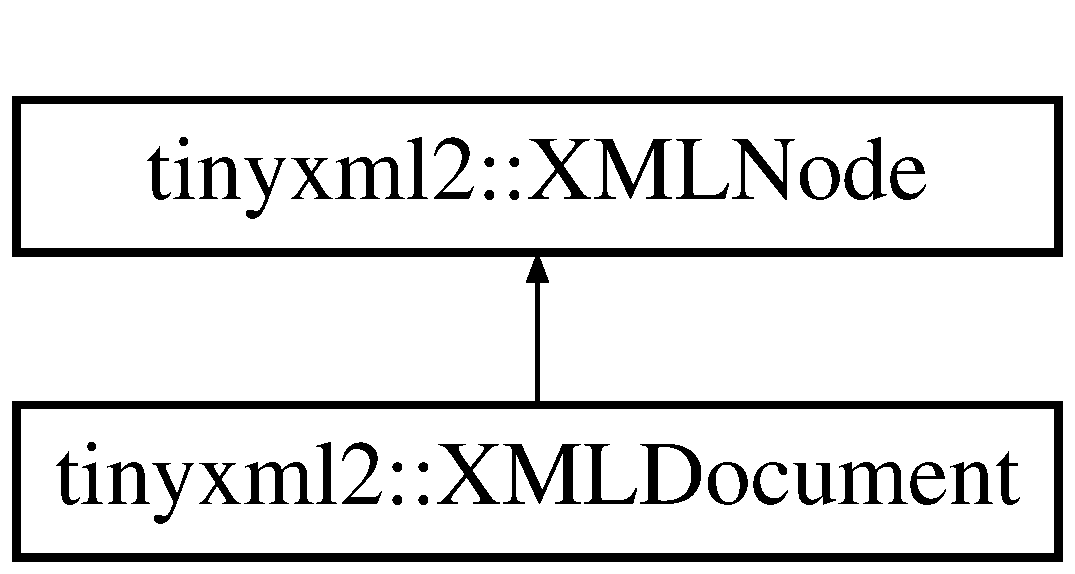
\includegraphics[height=2.000000cm]{classtinyxml2_1_1_x_m_l_document}
\end{center}
\end{figure}
\subsection*{Classes}
\begin{DoxyCompactItemize}
\item 
class \textbf{ Depth\+Tracker}
\end{DoxyCompactItemize}
\subsection*{Public Member Functions}
\begin{DoxyCompactItemize}
\item 
\textbf{ X\+M\+L\+Document} (bool process\+Entities=true, \textbf{ Whitespace} whitespace\+Mode=\textbf{ P\+R\+E\+S\+E\+R\+V\+E\+\_\+\+W\+H\+I\+T\+E\+S\+P\+A\+CE})
\begin{DoxyCompactList}\small\item\em constructor \end{DoxyCompactList}\item 
\textbf{ $\sim$\+X\+M\+L\+Document} ()
\item 
virtual \textbf{ X\+M\+L\+Document} $\ast$ \textbf{ To\+Document} ()
\begin{DoxyCompactList}\small\item\em Safely cast to a Document, or null. \end{DoxyCompactList}\item 
virtual const \textbf{ X\+M\+L\+Document} $\ast$ \textbf{ To\+Document} () const
\item 
\textbf{ X\+M\+L\+Error} \textbf{ Parse} (const char $\ast$xml, size\+\_\+t n\+Bytes=(size\+\_\+t)(-\/1))
\item 
\textbf{ X\+M\+L\+Error} \textbf{ Load\+File} (const char $\ast$filename)
\item 
\textbf{ X\+M\+L\+Error} \textbf{ Load\+File} (F\+I\+LE $\ast$)
\item 
\textbf{ X\+M\+L\+Error} \textbf{ Save\+File} (const char $\ast$filename, bool compact=false)
\item 
\textbf{ X\+M\+L\+Error} \textbf{ Save\+File} (F\+I\+LE $\ast$fp, bool compact=false)
\item 
bool \textbf{ Process\+Entities} () const
\item 
\textbf{ Whitespace} \textbf{ Whitespace\+Mode} () const
\item 
bool \textbf{ Has\+B\+OM} () const
\item 
void \textbf{ Set\+B\+OM} (bool use\+B\+OM)
\item 
\textbf{ X\+M\+L\+Element} $\ast$ \textbf{ Root\+Element} ()
\item 
const \textbf{ X\+M\+L\+Element} $\ast$ \textbf{ Root\+Element} () const
\item 
void \textbf{ Print} (\textbf{ X\+M\+L\+Printer} $\ast$streamer=0) const
\item 
virtual bool \textbf{ Accept} (\textbf{ X\+M\+L\+Visitor} $\ast$visitor) const
\item 
\textbf{ X\+M\+L\+Element} $\ast$ \textbf{ New\+Element} (const char $\ast$name)
\item 
\textbf{ X\+M\+L\+Comment} $\ast$ \textbf{ New\+Comment} (const char $\ast$comment)
\item 
\textbf{ X\+M\+L\+Text} $\ast$ \textbf{ New\+Text} (const char $\ast$text)
\item 
\textbf{ X\+M\+L\+Declaration} $\ast$ \textbf{ New\+Declaration} (const char $\ast$text=0)
\item 
\textbf{ X\+M\+L\+Unknown} $\ast$ \textbf{ New\+Unknown} (const char $\ast$text)
\item 
void \textbf{ Delete\+Node} (\textbf{ X\+M\+L\+Node} $\ast$node)
\item 
void \textbf{ Clear\+Error} ()
\item 
bool \textbf{ Error} () const
\begin{DoxyCompactList}\small\item\em Return true if there was an error parsing the document. \end{DoxyCompactList}\item 
\textbf{ X\+M\+L\+Error} \textbf{ Error\+ID} () const
\begin{DoxyCompactList}\small\item\em Return the error\+ID. \end{DoxyCompactList}\item 
const char $\ast$ \textbf{ Error\+Name} () const
\item 
const char $\ast$ \textbf{ Error\+Str} () const
\item 
void \textbf{ Print\+Error} () const
\begin{DoxyCompactList}\small\item\em A (trivial) utility function that prints the \doxyref{Error\+Str()}{p.}{classtinyxml2_1_1_x_m_l_document_ae97fff2402a0d01e0509c430b37996b3} to stdout. \end{DoxyCompactList}\item 
int \textbf{ Error\+Line\+Num} () const
\begin{DoxyCompactList}\small\item\em Return the line where the error occurred, or zero if unknown. \end{DoxyCompactList}\item 
void \textbf{ Clear} ()
\begin{DoxyCompactList}\small\item\em Clear the document, resetting it to the initial state. \end{DoxyCompactList}\item 
void \textbf{ Deep\+Copy} (\textbf{ X\+M\+L\+Document} $\ast$target) const
\item 
char $\ast$ \textbf{ Identify} (char $\ast$p, \textbf{ X\+M\+L\+Node} $\ast$$\ast$node)
\item 
void \textbf{ Mark\+In\+Use} (\textbf{ X\+M\+L\+Node} $\ast$)
\item 
virtual \textbf{ X\+M\+L\+Node} $\ast$ \textbf{ Shallow\+Clone} (\textbf{ X\+M\+L\+Document} $\ast$) const
\item 
virtual bool \textbf{ Shallow\+Equal} (const \textbf{ X\+M\+L\+Node} $\ast$) const
\end{DoxyCompactItemize}
\subsection*{Static Public Member Functions}
\begin{DoxyCompactItemize}
\item 
static const char $\ast$ \textbf{ Error\+I\+D\+To\+Name} (\textbf{ X\+M\+L\+Error} error\+ID)
\end{DoxyCompactItemize}
\subsection*{Private Member Functions}
\begin{DoxyCompactItemize}
\item 
\textbf{ X\+M\+L\+Document} (const \textbf{ X\+M\+L\+Document} \&)
\item 
void \textbf{ operator=} (const \textbf{ X\+M\+L\+Document} \&)
\item 
void \textbf{ Parse} ()
\item 
void \textbf{ Set\+Error} (\textbf{ X\+M\+L\+Error} error, int line\+Num, const char $\ast$format,...)
\item 
void \textbf{ Push\+Depth} ()
\item 
void \textbf{ Pop\+Depth} ()
\item 
{\footnotesize template$<$class Node\+Type , int Pool\+Element\+Size$>$ }\\Node\+Type $\ast$ \textbf{ Create\+Unlinked\+Node} (\textbf{ Mem\+PoolT}$<$ Pool\+Element\+Size $>$ \&pool)
\end{DoxyCompactItemize}
\subsection*{Private Attributes}
\begin{DoxyCompactItemize}
\item 
bool \textbf{ \+\_\+write\+B\+OM}
\item 
bool \textbf{ \+\_\+process\+Entities}
\item 
\textbf{ X\+M\+L\+Error} \textbf{ \+\_\+error\+ID}
\item 
\textbf{ Whitespace} \textbf{ \+\_\+whitespace\+Mode}
\item 
\textbf{ Str\+Pair} \textbf{ \+\_\+error\+Str}
\item 
int \textbf{ \+\_\+error\+Line\+Num}
\item 
char $\ast$ \textbf{ \+\_\+char\+Buffer}
\item 
int \textbf{ \+\_\+parse\+Cur\+Line\+Num}
\item 
int \textbf{ \+\_\+parsing\+Depth}
\item 
\textbf{ Dyn\+Array}$<$ \textbf{ X\+M\+L\+Node} $\ast$, 10 $>$ \textbf{ \+\_\+unlinked}
\item 
\textbf{ Mem\+PoolT}$<$ sizeof(\textbf{ X\+M\+L\+Element}) $>$ \textbf{ \+\_\+element\+Pool}
\item 
\textbf{ Mem\+PoolT}$<$ sizeof(\textbf{ X\+M\+L\+Attribute}) $>$ \textbf{ \+\_\+attribute\+Pool}
\item 
\textbf{ Mem\+PoolT}$<$ sizeof(\textbf{ X\+M\+L\+Text}) $>$ \textbf{ \+\_\+text\+Pool}
\item 
\textbf{ Mem\+PoolT}$<$ sizeof(\textbf{ X\+M\+L\+Comment}) $>$ \textbf{ \+\_\+comment\+Pool}
\end{DoxyCompactItemize}
\subsection*{Static Private Attributes}
\begin{DoxyCompactItemize}
\item 
static const char $\ast$ \textbf{ \+\_\+error\+Names} [\textbf{ X\+M\+L\+\_\+\+E\+R\+R\+O\+R\+\_\+\+C\+O\+U\+NT}]
\end{DoxyCompactItemize}
\subsection*{Friends}
\begin{DoxyCompactItemize}
\item 
class \textbf{ X\+M\+L\+Element}
\item 
class \textbf{ X\+M\+L\+Node}
\item 
class \textbf{ X\+M\+L\+Text}
\item 
class \textbf{ X\+M\+L\+Comment}
\item 
class \textbf{ X\+M\+L\+Declaration}
\item 
class \textbf{ X\+M\+L\+Unknown}
\end{DoxyCompactItemize}
\subsection*{Additional Inherited Members}


\subsection{Detailed Description}
A Document binds together all the functionality. It can be saved, loaded, and printed to the screen. All Nodes are connected and allocated to a Document. If the Document is deleted, all its Nodes are also deleted. 

Definition at line 1653 of file tinyxml2.\+h.



\subsection{Constructor \& Destructor Documentation}
\mbox{\label{classtinyxml2_1_1_x_m_l_document_a57ddf17b6e054dda10af98991b1b8f70}} 
\index{tinyxml2::XMLDocument@{tinyxml2::XMLDocument}!XMLDocument@{XMLDocument}}
\index{XMLDocument@{XMLDocument}!tinyxml2::XMLDocument@{tinyxml2::XMLDocument}}
\subsubsection{XMLDocument()\hspace{0.1cm}{\footnotesize\ttfamily [1/2]}}
{\footnotesize\ttfamily tinyxml2\+::\+X\+M\+L\+Document\+::\+X\+M\+L\+Document (\begin{DoxyParamCaption}\item[{bool}]{process\+Entities = {\ttfamily true},  }\item[{\textbf{ Whitespace}}]{whitespace\+Mode = {\ttfamily \textbf{ P\+R\+E\+S\+E\+R\+V\+E\+\_\+\+W\+H\+I\+T\+E\+S\+P\+A\+CE}} }\end{DoxyParamCaption})}



constructor 



Definition at line 2006 of file tinyxml2.\+cpp.



References tinyxml2\+::\+X\+M\+L\+Node\+::\+\_\+document.

\mbox{\label{classtinyxml2_1_1_x_m_l_document_af37c47d8e2ba4b2fc81b21a77a32579b}} 
\index{tinyxml2::XMLDocument@{tinyxml2::XMLDocument}!````~XMLDocument@{$\sim$XMLDocument}}
\index{````~XMLDocument@{$\sim$XMLDocument}!tinyxml2::XMLDocument@{tinyxml2::XMLDocument}}
\subsubsection{$\sim$XMLDocument()}
{\footnotesize\ttfamily tinyxml2\+::\+X\+M\+L\+Document\+::$\sim$\+X\+M\+L\+Document (\begin{DoxyParamCaption}{ }\end{DoxyParamCaption})}



Definition at line 2028 of file tinyxml2.\+cpp.



References Clear().

\mbox{\label{classtinyxml2_1_1_x_m_l_document_adcea490db02a099d99440cd14a87d9e4}} 
\index{tinyxml2::XMLDocument@{tinyxml2::XMLDocument}!XMLDocument@{XMLDocument}}
\index{XMLDocument@{XMLDocument}!tinyxml2::XMLDocument@{tinyxml2::XMLDocument}}
\subsubsection{XMLDocument()\hspace{0.1cm}{\footnotesize\ttfamily [2/2]}}
{\footnotesize\ttfamily tinyxml2\+::\+X\+M\+L\+Document\+::\+X\+M\+L\+Document (\begin{DoxyParamCaption}\item[{const \textbf{ X\+M\+L\+Document} \&}]{ }\end{DoxyParamCaption})\hspace{0.3cm}{\ttfamily [private]}}



\subsection{Member Function Documentation}
\mbox{\label{classtinyxml2_1_1_x_m_l_document_ab7be651917a35ab1ff0e4e6d4e565cdf}} 
\index{tinyxml2::XMLDocument@{tinyxml2::XMLDocument}!Accept@{Accept}}
\index{Accept@{Accept}!tinyxml2::XMLDocument@{tinyxml2::XMLDocument}}
\subsubsection{Accept()}
{\footnotesize\ttfamily bool tinyxml2\+::\+X\+M\+L\+Document\+::\+Accept (\begin{DoxyParamCaption}\item[{\textbf{ X\+M\+L\+Visitor} $\ast$}]{visitor }\end{DoxyParamCaption}) const\hspace{0.3cm}{\ttfamily [virtual]}}

Accept a hierarchical visit of the nodes in the Tiny\+X\+M\+L-\/2 D\+OM. Every node in the X\+ML tree will be conditionally visited and the host will be called back via the \doxyref{X\+M\+L\+Visitor}{p.}{classtinyxml2_1_1_x_m_l_visitor} interface.

This is essentially a S\+AX interface for Tiny\+X\+M\+L-\/2. (Note however it doesn\textquotesingle{}t re-\/parse the X\+ML for the callbacks, so the performance of Tiny\+X\+M\+L-\/2 is unchanged by using this interface versus any other.)

The interface has been based on ideas from\+:


\begin{DoxyItemize}
\item {\texttt{ http\+://www.\+saxproject.\+org/}}
\item {\texttt{ http\+://c2.\+com/cgi/wiki?\+Hierarchical\+Visitor\+Pattern}}
\end{DoxyItemize}

Which are both good references for \char`\"{}visiting\char`\"{}.

An example of using \doxyref{Accept()}{p.}{classtinyxml2_1_1_x_m_l_document_ab7be651917a35ab1ff0e4e6d4e565cdf}\+: \begin{DoxyVerb}XMLPrinter printer;
tinyxmlDoc.Accept( &printer );
const char* xmlcstr = printer.CStr();
\end{DoxyVerb}
 

Implements \textbf{ tinyxml2\+::\+X\+M\+L\+Node} \doxyref{}{p.}{classtinyxml2_1_1_x_m_l_node_a81e66df0a44c67a7af17f3b77a152785}.



Definition at line 726 of file tinyxml2.\+cpp.



References tinyxml2\+::\+X\+M\+L\+Node\+::\+First\+Child(), tinyxml2\+::\+X\+M\+L\+Node\+::\+Next\+Sibling(), T\+I\+X\+M\+L\+A\+S\+S\+E\+RT, tinyxml2\+::\+X\+M\+L\+Visitor\+::\+Visit\+Enter(), and tinyxml2\+::\+X\+M\+L\+Visitor\+::\+Visit\+Exit().



Referenced by Print().

\mbox{\label{classtinyxml2_1_1_x_m_l_document_a65656b0b2cbc822708eb351504178aaf}} 
\index{tinyxml2::XMLDocument@{tinyxml2::XMLDocument}!Clear@{Clear}}
\index{Clear@{Clear}!tinyxml2::XMLDocument@{tinyxml2::XMLDocument}}
\subsubsection{Clear()}
{\footnotesize\ttfamily void tinyxml2\+::\+X\+M\+L\+Document\+::\+Clear (\begin{DoxyParamCaption}{ }\end{DoxyParamCaption})}



Clear the document, resetting it to the initial state. 



Definition at line 2047 of file tinyxml2.\+cpp.



References \+\_\+attribute\+Pool, \+\_\+char\+Buffer, \+\_\+comment\+Pool, \+\_\+element\+Pool, \+\_\+parsing\+Depth, \+\_\+text\+Pool, \+\_\+unlinked, Clear\+Error(), tinyxml2\+::\+X\+M\+L\+Node\+::\+Delete\+Children(), Delete\+Node(), Error(), and T\+I\+X\+M\+L\+A\+S\+S\+E\+RT.



Referenced by Deep\+Copy(), Load\+File(), Parse(), and $\sim$\+X\+M\+L\+Document().

\mbox{\label{classtinyxml2_1_1_x_m_l_document_a4085d9c52f1d93214311459d6d1fcf17}} 
\index{tinyxml2::XMLDocument@{tinyxml2::XMLDocument}!ClearError@{ClearError}}
\index{ClearError@{ClearError}!tinyxml2::XMLDocument@{tinyxml2::XMLDocument}}
\subsubsection{ClearError()}
{\footnotesize\ttfamily void tinyxml2\+::\+X\+M\+L\+Document\+::\+Clear\+Error (\begin{DoxyParamCaption}{ }\end{DoxyParamCaption})\hspace{0.3cm}{\ttfamily [inline]}}



Definition at line 1814 of file tinyxml2.\+h.



References tinyxml2\+::\+X\+M\+L\+\_\+\+S\+U\+C\+C\+E\+SS.



Referenced by Clear(), and Save\+File().

\mbox{\label{classtinyxml2_1_1_x_m_l_document_acda2123b71a6e6534be9f48e75ea680a}} 
\index{tinyxml2::XMLDocument@{tinyxml2::XMLDocument}!CreateUnlinkedNode@{CreateUnlinkedNode}}
\index{CreateUnlinkedNode@{CreateUnlinkedNode}!tinyxml2::XMLDocument@{tinyxml2::XMLDocument}}
\subsubsection{CreateUnlinkedNode()}
{\footnotesize\ttfamily template$<$class Node\+Type , int Pool\+Element\+Size$>$ \\
Node\+Type $\ast$ tinyxml2\+::\+X\+M\+L\+Document\+::\+Create\+Unlinked\+Node (\begin{DoxyParamCaption}\item[{\textbf{ Mem\+PoolT}$<$ Pool\+Element\+Size $>$ \&}]{pool }\end{DoxyParamCaption})\hspace{0.3cm}{\ttfamily [inline]}, {\ttfamily [private]}}



Definition at line 1923 of file tinyxml2.\+h.



References \+\_\+unlinked, tinyxml2\+::\+Mem\+Pool\+T$<$ I\+T\+E\+M\+\_\+\+S\+I\+Z\+E $>$\+::\+Alloc(), tinyxml2\+::\+Mem\+Pool\+T$<$ I\+T\+E\+M\+\_\+\+S\+I\+Z\+E $>$\+::\+Item\+Size(), and T\+I\+X\+M\+L\+A\+S\+S\+E\+RT.

\mbox{\label{classtinyxml2_1_1_x_m_l_document_af592ffc91514e25a39664521ac83db45}} 
\index{tinyxml2::XMLDocument@{tinyxml2::XMLDocument}!DeepCopy@{DeepCopy}}
\index{DeepCopy@{DeepCopy}!tinyxml2::XMLDocument@{tinyxml2::XMLDocument}}
\subsubsection{DeepCopy()}
{\footnotesize\ttfamily void tinyxml2\+::\+X\+M\+L\+Document\+::\+Deep\+Copy (\begin{DoxyParamCaption}\item[{\textbf{ X\+M\+L\+Document} $\ast$}]{target }\end{DoxyParamCaption}) const}

Copies this document to a target document. The target will be completely cleared before the copy. If you want to copy a sub-\/tree, see \doxyref{X\+M\+L\+Node\+::\+Deep\+Clone()}{p.}{classtinyxml2_1_1_x_m_l_node_a3bb369fd733f1989b751d99a9417adab}.

N\+O\+TE\+: that the \textquotesingle{}target\textquotesingle{} must be non-\/null. 

Definition at line 2081 of file tinyxml2.\+cpp.



References Clear(), tinyxml2\+::\+X\+M\+L\+Node\+::\+First\+Child(), tinyxml2\+::\+X\+M\+L\+Node\+::\+Insert\+End\+Child(), tinyxml2\+::\+X\+M\+L\+Node\+::\+Next\+Sibling(), and T\+I\+X\+M\+L\+A\+S\+S\+E\+RT.

\mbox{\label{classtinyxml2_1_1_x_m_l_document_ac1d6e2c7fcc1a660624ac4f68e96380d}} 
\index{tinyxml2::XMLDocument@{tinyxml2::XMLDocument}!DeleteNode@{DeleteNode}}
\index{DeleteNode@{DeleteNode}!tinyxml2::XMLDocument@{tinyxml2::XMLDocument}}
\subsubsection{DeleteNode()}
{\footnotesize\ttfamily void tinyxml2\+::\+X\+M\+L\+Document\+::\+Delete\+Node (\begin{DoxyParamCaption}\item[{\textbf{ X\+M\+L\+Node} $\ast$}]{node }\end{DoxyParamCaption})}

Delete a node associated with this document. It will be unlinked from the D\+OM. 

Definition at line 2149 of file tinyxml2.\+cpp.



References tinyxml2\+::\+X\+M\+L\+Node\+::\+\_\+document, tinyxml2\+::\+X\+M\+L\+Node\+::\+\_\+mem\+Pool, tinyxml2\+::\+X\+M\+L\+Node\+::\+\_\+parent, tinyxml2\+::\+X\+M\+L\+Node\+::\+Delete\+Child(), tinyxml2\+::\+X\+M\+L\+Node\+::\+Delete\+Node(), tinyxml2\+::\+Mem\+Pool\+::\+Set\+Tracked(), and T\+I\+X\+M\+L\+A\+S\+S\+E\+RT.



Referenced by Clear().

\mbox{\label{classtinyxml2_1_1_x_m_l_document_a34e6318e182e40e3cc4f4ba5d59ed9ed}} 
\index{tinyxml2::XMLDocument@{tinyxml2::XMLDocument}!Error@{Error}}
\index{Error@{Error}!tinyxml2::XMLDocument@{tinyxml2::XMLDocument}}
\subsubsection{Error()}
{\footnotesize\ttfamily bool tinyxml2\+::\+X\+M\+L\+Document\+::\+Error (\begin{DoxyParamCaption}{ }\end{DoxyParamCaption}) const\hspace{0.3cm}{\ttfamily [inline]}}



Return true if there was an error parsing the document. 



Definition at line 1819 of file tinyxml2.\+h.



References tinyxml2\+::\+X\+M\+L\+\_\+\+S\+U\+C\+C\+E\+SS.



Referenced by Clear(), Parse(), and tinyxml2\+::\+X\+M\+L\+Node\+::\+Parse\+Deep().

\mbox{\label{classtinyxml2_1_1_x_m_l_document_afa3ed33b3107f920ec2b301f805ac17d}} 
\index{tinyxml2::XMLDocument@{tinyxml2::XMLDocument}!ErrorID@{ErrorID}}
\index{ErrorID@{ErrorID}!tinyxml2::XMLDocument@{tinyxml2::XMLDocument}}
\subsubsection{ErrorID()}
{\footnotesize\ttfamily \textbf{ X\+M\+L\+Error} tinyxml2\+::\+X\+M\+L\+Document\+::\+Error\+ID (\begin{DoxyParamCaption}{ }\end{DoxyParamCaption}) const\hspace{0.3cm}{\ttfamily [inline]}}



Return the error\+ID. 



Definition at line 1823 of file tinyxml2.\+h.

\mbox{\label{classtinyxml2_1_1_x_m_l_document_a639f7c295c38dc5a4aafeb2fff93da03}} 
\index{tinyxml2::XMLDocument@{tinyxml2::XMLDocument}!ErrorIDToName@{ErrorIDToName}}
\index{ErrorIDToName@{ErrorIDToName}!tinyxml2::XMLDocument@{tinyxml2::XMLDocument}}
\subsubsection{ErrorIDToName()}
{\footnotesize\ttfamily const char $\ast$ tinyxml2\+::\+X\+M\+L\+Document\+::\+Error\+I\+D\+To\+Name (\begin{DoxyParamCaption}\item[{\textbf{ X\+M\+L\+Error}}]{error\+ID }\end{DoxyParamCaption})\hspace{0.3cm}{\ttfamily [static]}}



Definition at line 2356 of file tinyxml2.\+cpp.



References \+\_\+error\+Names, T\+I\+X\+M\+L\+A\+S\+S\+E\+RT, and tinyxml2\+::\+X\+M\+L\+\_\+\+E\+R\+R\+O\+R\+\_\+\+C\+O\+U\+NT.



Referenced by Error\+Name(), and Set\+Error().

\mbox{\label{classtinyxml2_1_1_x_m_l_document_a57400f816dbe7799ece33615ead9ab76}} 
\index{tinyxml2::XMLDocument@{tinyxml2::XMLDocument}!ErrorLineNum@{ErrorLineNum}}
\index{ErrorLineNum@{ErrorLineNum}!tinyxml2::XMLDocument@{tinyxml2::XMLDocument}}
\subsubsection{ErrorLineNum()}
{\footnotesize\ttfamily int tinyxml2\+::\+X\+M\+L\+Document\+::\+Error\+Line\+Num (\begin{DoxyParamCaption}{ }\end{DoxyParamCaption}) const\hspace{0.3cm}{\ttfamily [inline]}}



Return the line where the error occurred, or zero if unknown. 



Definition at line 1838 of file tinyxml2.\+h.

\mbox{\label{classtinyxml2_1_1_x_m_l_document_a1a5f2b63427caffd4cde15781d9d11f9}} 
\index{tinyxml2::XMLDocument@{tinyxml2::XMLDocument}!ErrorName@{ErrorName}}
\index{ErrorName@{ErrorName}!tinyxml2::XMLDocument@{tinyxml2::XMLDocument}}
\subsubsection{ErrorName()}
{\footnotesize\ttfamily const char $\ast$ tinyxml2\+::\+X\+M\+L\+Document\+::\+Error\+Name (\begin{DoxyParamCaption}{ }\end{DoxyParamCaption}) const}



Definition at line 2375 of file tinyxml2.\+cpp.



References \+\_\+error\+ID, and Error\+I\+D\+To\+Name().

\mbox{\label{classtinyxml2_1_1_x_m_l_document_ae97fff2402a0d01e0509c430b37996b3}} 
\index{tinyxml2::XMLDocument@{tinyxml2::XMLDocument}!ErrorStr@{ErrorStr}}
\index{ErrorStr@{ErrorStr}!tinyxml2::XMLDocument@{tinyxml2::XMLDocument}}
\subsubsection{ErrorStr()}
{\footnotesize\ttfamily const char $\ast$ tinyxml2\+::\+X\+M\+L\+Document\+::\+Error\+Str (\begin{DoxyParamCaption}{ }\end{DoxyParamCaption}) const}

Returns a \char`\"{}long form\char`\"{} error description. A hopefully helpful diagnostic with location, line number, and/or additional info. 

Definition at line 2364 of file tinyxml2.\+cpp.



References \+\_\+error\+Str, tinyxml2\+::\+Str\+Pair\+::\+Empty(), and tinyxml2\+::\+Str\+Pair\+::\+Get\+Str().



Referenced by Print\+Error().

\mbox{\label{classtinyxml2_1_1_x_m_l_document_a33fc5d159db873a179fa26338adb05bd}} 
\index{tinyxml2::XMLDocument@{tinyxml2::XMLDocument}!HasBOM@{HasBOM}}
\index{HasBOM@{HasBOM}!tinyxml2::XMLDocument@{tinyxml2::XMLDocument}}
\subsubsection{HasBOM()}
{\footnotesize\ttfamily bool tinyxml2\+::\+X\+M\+L\+Document\+::\+Has\+B\+OM (\begin{DoxyParamCaption}{ }\end{DoxyParamCaption}) const\hspace{0.3cm}{\ttfamily [inline]}}

Returns true if this document has a leading Byte Order Mark of U\+T\+F8. 

Definition at line 1735 of file tinyxml2.\+h.



Referenced by tinyxml2\+::\+X\+M\+L\+Printer\+::\+Visit\+Enter().

\mbox{\label{classtinyxml2_1_1_x_m_l_document_a25827d1bec509ad566a107e5853ed040}} 
\index{tinyxml2::XMLDocument@{tinyxml2::XMLDocument}!Identify@{Identify}}
\index{Identify@{Identify}!tinyxml2::XMLDocument@{tinyxml2::XMLDocument}}
\subsubsection{Identify()}
{\footnotesize\ttfamily char $\ast$ tinyxml2\+::\+X\+M\+L\+Document\+::\+Identify (\begin{DoxyParamCaption}\item[{char $\ast$}]{p,  }\item[{\textbf{ X\+M\+L\+Node} $\ast$$\ast$}]{node }\end{DoxyParamCaption})}



Definition at line 656 of file tinyxml2.\+cpp.



References \+\_\+comment\+Pool, \+\_\+element\+Pool, \+\_\+parse\+Cur\+Line\+Num, tinyxml2\+::\+X\+M\+L\+Node\+::\+\_\+parse\+Line\+Num, \+\_\+text\+Pool, tinyxml2\+::\+X\+M\+L\+Text\+::\+Set\+C\+Data(), tinyxml2\+::\+X\+M\+L\+Util\+::\+Skip\+White\+Space(), tinyxml2\+::\+X\+M\+L\+Util\+::\+String\+Equal(), and T\+I\+X\+M\+L\+A\+S\+S\+E\+RT.



Referenced by tinyxml2\+::\+X\+M\+L\+Node\+::\+Parse\+Deep().

\mbox{\label{classtinyxml2_1_1_x_m_l_document_a2ebd4647a8af5fc6831b294ac26a150a}} 
\index{tinyxml2::XMLDocument@{tinyxml2::XMLDocument}!LoadFile@{LoadFile}}
\index{LoadFile@{LoadFile}!tinyxml2::XMLDocument@{tinyxml2::XMLDocument}}
\subsubsection{LoadFile()\hspace{0.1cm}{\footnotesize\ttfamily [1/2]}}
{\footnotesize\ttfamily \textbf{ X\+M\+L\+Error} tinyxml2\+::\+X\+M\+L\+Document\+::\+Load\+File (\begin{DoxyParamCaption}\item[{const char $\ast$}]{filename }\end{DoxyParamCaption})}

Load an X\+ML file from disk. Returns X\+M\+L\+\_\+\+S\+U\+C\+C\+E\+SS (0) on success, or an error\+ID. 

Definition at line 2167 of file tinyxml2.\+cpp.



References \+\_\+error\+ID, tinyxml2\+::callfopen(), Clear(), Set\+Error(), T\+I\+X\+M\+L\+A\+S\+S\+E\+RT, tinyxml2\+::\+X\+M\+L\+\_\+\+E\+R\+R\+O\+R\+\_\+\+F\+I\+L\+E\+\_\+\+C\+O\+U\+L\+D\+\_\+\+N\+O\+T\+\_\+\+B\+E\+\_\+\+O\+P\+E\+N\+ED, and tinyxml2\+::\+X\+M\+L\+\_\+\+E\+R\+R\+O\+R\+\_\+\+F\+I\+L\+E\+\_\+\+N\+O\+T\+\_\+\+F\+O\+U\+ND.



Referenced by World\+::parse\+Antennas(), World\+::parse\+Persons(), and World\+::parse\+Simulation\+File().

\mbox{\label{classtinyxml2_1_1_x_m_l_document_a5f1d330fad44c52f3d265338dd2a6dc2}} 
\index{tinyxml2::XMLDocument@{tinyxml2::XMLDocument}!LoadFile@{LoadFile}}
\index{LoadFile@{LoadFile}!tinyxml2::XMLDocument@{tinyxml2::XMLDocument}}
\subsubsection{LoadFile()\hspace{0.1cm}{\footnotesize\ttfamily [2/2]}}
{\footnotesize\ttfamily \textbf{ X\+M\+L\+Error} tinyxml2\+::\+X\+M\+L\+Document\+::\+Load\+File (\begin{DoxyParamCaption}\item[{F\+I\+LE $\ast$}]{fp }\end{DoxyParamCaption})}

Load an X\+ML file from disk. You are responsible for providing and closing the F\+I\+L\+E$\ast$.

N\+O\+TE\+: The file should be opened as binary (\char`\"{}rb\char`\"{}) not text in order for Tiny\+X\+M\+L-\/2 to correctly do newline normalization.

Returns X\+M\+L\+\_\+\+S\+U\+C\+C\+E\+SS (0) on success, or an error\+ID. 

Definition at line 2209 of file tinyxml2.\+cpp.



References \+\_\+char\+Buffer, \+\_\+error\+ID, Clear(), Parse(), Set\+Error(), T\+I\+X\+M\+L\+A\+S\+S\+E\+RT, tinyxml2\+::\+X\+M\+L\+\_\+\+E\+R\+R\+O\+R\+\_\+\+E\+M\+P\+T\+Y\+\_\+\+D\+O\+C\+U\+M\+E\+NT, and tinyxml2\+::\+X\+M\+L\+\_\+\+E\+R\+R\+O\+R\+\_\+\+F\+I\+L\+E\+\_\+\+R\+E\+A\+D\+\_\+\+E\+R\+R\+OR.

\mbox{\label{classtinyxml2_1_1_x_m_l_document_a95d28ecb4760a994556b0a51690b21be}} 
\index{tinyxml2::XMLDocument@{tinyxml2::XMLDocument}!MarkInUse@{MarkInUse}}
\index{MarkInUse@{MarkInUse}!tinyxml2::XMLDocument@{tinyxml2::XMLDocument}}
\subsubsection{MarkInUse()}
{\footnotesize\ttfamily void tinyxml2\+::\+X\+M\+L\+Document\+::\+Mark\+In\+Use (\begin{DoxyParamCaption}\item[{\textbf{ X\+M\+L\+Node} $\ast$}]{node }\end{DoxyParamCaption})}



Definition at line 2034 of file tinyxml2.\+cpp.



References tinyxml2\+::\+X\+M\+L\+Node\+::\+\_\+parent, \+\_\+unlinked, and T\+I\+X\+M\+L\+A\+S\+S\+E\+RT.



Referenced by tinyxml2\+::\+X\+M\+L\+Node\+::\+Delete\+Node(), and tinyxml2\+::\+X\+M\+L\+Node\+::\+Insert\+Child\+Preamble().

\mbox{\label{classtinyxml2_1_1_x_m_l_document_a386df0befd06aadb5e0cd21381aa955a}} 
\index{tinyxml2::XMLDocument@{tinyxml2::XMLDocument}!NewComment@{NewComment}}
\index{NewComment@{NewComment}!tinyxml2::XMLDocument@{tinyxml2::XMLDocument}}
\subsubsection{NewComment()}
{\footnotesize\ttfamily \textbf{ X\+M\+L\+Comment} $\ast$ tinyxml2\+::\+X\+M\+L\+Document\+::\+New\+Comment (\begin{DoxyParamCaption}\item[{const char $\ast$}]{comment }\end{DoxyParamCaption})}

Create a new Comment associated with this Document. The memory for the Comment is managed by the Document. 

Definition at line 2102 of file tinyxml2.\+cpp.



References \+\_\+comment\+Pool, and tinyxml2\+::\+X\+M\+L\+Node\+::\+Set\+Value().



Referenced by tinyxml2\+::\+X\+M\+L\+Comment\+::\+Shallow\+Clone().

\mbox{\label{classtinyxml2_1_1_x_m_l_document_ae519030c0262fa2daff8993681990e16}} 
\index{tinyxml2::XMLDocument@{tinyxml2::XMLDocument}!NewDeclaration@{NewDeclaration}}
\index{NewDeclaration@{NewDeclaration}!tinyxml2::XMLDocument@{tinyxml2::XMLDocument}}
\subsubsection{NewDeclaration()}
{\footnotesize\ttfamily \textbf{ X\+M\+L\+Declaration} $\ast$ tinyxml2\+::\+X\+M\+L\+Document\+::\+New\+Declaration (\begin{DoxyParamCaption}\item[{const char $\ast$}]{text = {\ttfamily 0} }\end{DoxyParamCaption})}

Create a new Declaration associated with this Document. The memory for the object is managed by the Document.

If the \textquotesingle{}text\textquotesingle{} param is null, the standard declaration is used.\+: \begin{DoxyVerb}    <?xml version="1.0" encoding="UTF-8"?>
\end{DoxyVerb}
 

Definition at line 2118 of file tinyxml2.\+cpp.



References \+\_\+comment\+Pool, and tinyxml2\+::\+X\+M\+L\+Node\+::\+Set\+Value().



Referenced by tinyxml2\+::\+X\+M\+L\+Declaration\+::\+Shallow\+Clone().

\mbox{\label{classtinyxml2_1_1_x_m_l_document_a3c335a700a43d7c363a393142a23f234}} 
\index{tinyxml2::XMLDocument@{tinyxml2::XMLDocument}!NewElement@{NewElement}}
\index{NewElement@{NewElement}!tinyxml2::XMLDocument@{tinyxml2::XMLDocument}}
\subsubsection{NewElement()}
{\footnotesize\ttfamily \textbf{ X\+M\+L\+Element} $\ast$ tinyxml2\+::\+X\+M\+L\+Document\+::\+New\+Element (\begin{DoxyParamCaption}\item[{const char $\ast$}]{name }\end{DoxyParamCaption})}

Create a new Element associated with this Document. The memory for the Element is managed by the Document. 

Definition at line 2094 of file tinyxml2.\+cpp.



References \+\_\+element\+Pool, and tinyxml2\+::\+X\+M\+L\+Element\+::\+Set\+Name().



Referenced by tinyxml2\+::\+X\+M\+L\+Element\+::\+Shallow\+Clone().

\mbox{\label{classtinyxml2_1_1_x_m_l_document_acece5de77a0819f2341b08c1e1ed9987}} 
\index{tinyxml2::XMLDocument@{tinyxml2::XMLDocument}!NewText@{NewText}}
\index{NewText@{NewText}!tinyxml2::XMLDocument@{tinyxml2::XMLDocument}}
\subsubsection{NewText()}
{\footnotesize\ttfamily \textbf{ X\+M\+L\+Text} $\ast$ tinyxml2\+::\+X\+M\+L\+Document\+::\+New\+Text (\begin{DoxyParamCaption}\item[{const char $\ast$}]{text }\end{DoxyParamCaption})}

Create a new Text associated with this Document. The memory for the Text is managed by the Document. 

Definition at line 2110 of file tinyxml2.\+cpp.



References \+\_\+text\+Pool, and tinyxml2\+::\+X\+M\+L\+Node\+::\+Set\+Value().



Referenced by tinyxml2\+::\+X\+M\+L\+Element\+::\+Set\+Text(), and tinyxml2\+::\+X\+M\+L\+Text\+::\+Shallow\+Clone().

\mbox{\label{classtinyxml2_1_1_x_m_l_document_a4954f502c5fd7f49de54c3c0c99bb73d}} 
\index{tinyxml2::XMLDocument@{tinyxml2::XMLDocument}!NewUnknown@{NewUnknown}}
\index{NewUnknown@{NewUnknown}!tinyxml2::XMLDocument@{tinyxml2::XMLDocument}}
\subsubsection{NewUnknown()}
{\footnotesize\ttfamily \textbf{ X\+M\+L\+Unknown} $\ast$ tinyxml2\+::\+X\+M\+L\+Document\+::\+New\+Unknown (\begin{DoxyParamCaption}\item[{const char $\ast$}]{text }\end{DoxyParamCaption})}

Create a new Unknown associated with this Document. The memory for the object is managed by the Document. 

Definition at line 2126 of file tinyxml2.\+cpp.



References \+\_\+comment\+Pool, and tinyxml2\+::\+X\+M\+L\+Node\+::\+Set\+Value().



Referenced by tinyxml2\+::\+X\+M\+L\+Unknown\+::\+Shallow\+Clone().

\mbox{\label{classtinyxml2_1_1_x_m_l_document_aa542c2cf1276ee4bd778f16d196fe222}} 
\index{tinyxml2::XMLDocument@{tinyxml2::XMLDocument}!operator=@{operator=}}
\index{operator=@{operator=}!tinyxml2::XMLDocument@{tinyxml2::XMLDocument}}
\subsubsection{operator=()}
{\footnotesize\ttfamily void tinyxml2\+::\+X\+M\+L\+Document\+::operator= (\begin{DoxyParamCaption}\item[{const \textbf{ X\+M\+L\+Document} \&}]{ }\end{DoxyParamCaption})\hspace{0.3cm}{\ttfamily [private]}}

\mbox{\label{classtinyxml2_1_1_x_m_l_document_a1819bd34f540a7304c105a6232d25a1f}} 
\index{tinyxml2::XMLDocument@{tinyxml2::XMLDocument}!Parse@{Parse}}
\index{Parse@{Parse}!tinyxml2::XMLDocument@{tinyxml2::XMLDocument}}
\subsubsection{Parse()\hspace{0.1cm}{\footnotesize\ttfamily [1/2]}}
{\footnotesize\ttfamily \textbf{ X\+M\+L\+Error} tinyxml2\+::\+X\+M\+L\+Document\+::\+Parse (\begin{DoxyParamCaption}\item[{const char $\ast$}]{xml,  }\item[{size\+\_\+t}]{n\+Bytes = {\ttfamily (size\+\_\+t)(-\/1)} }\end{DoxyParamCaption})}

Parse an X\+ML file from a character string. Returns X\+M\+L\+\_\+\+S\+U\+C\+C\+E\+SS (0) on success, or an error\+ID.

You may optionally pass in the \textquotesingle{}n\+Bytes\textquotesingle{}, which is the number of bytes which will be parsed. If not specified, Tiny\+X\+M\+L-\/2 will assume \textquotesingle{}xml\textquotesingle{} points to a null terminated string. 

Definition at line 2285 of file tinyxml2.\+cpp.



References \+\_\+attribute\+Pool, \+\_\+char\+Buffer, \+\_\+comment\+Pool, \+\_\+element\+Pool, \+\_\+error\+ID, \+\_\+text\+Pool, Clear(), tinyxml2\+::\+X\+M\+L\+Node\+::\+Delete\+Children(), Error(), Parse(), Set\+Error(), T\+I\+X\+M\+L\+A\+S\+S\+E\+RT, and tinyxml2\+::\+X\+M\+L\+\_\+\+E\+R\+R\+O\+R\+\_\+\+E\+M\+P\+T\+Y\+\_\+\+D\+O\+C\+U\+M\+E\+NT.

\mbox{\label{classtinyxml2_1_1_x_m_l_document_aeb556e0e2bed02a73a6c5aaf19759e9a}} 
\index{tinyxml2::XMLDocument@{tinyxml2::XMLDocument}!Parse@{Parse}}
\index{Parse@{Parse}!tinyxml2::XMLDocument@{tinyxml2::XMLDocument}}
\subsubsection{Parse()\hspace{0.1cm}{\footnotesize\ttfamily [2/2]}}
{\footnotesize\ttfamily void tinyxml2\+::\+X\+M\+L\+Document\+::\+Parse (\begin{DoxyParamCaption}{ }\end{DoxyParamCaption})\hspace{0.3cm}{\ttfamily [private]}}



Definition at line 2380 of file tinyxml2.\+cpp.



References \+\_\+char\+Buffer, \+\_\+parse\+Cur\+Line\+Num, tinyxml2\+::\+X\+M\+L\+Node\+::\+\_\+parse\+Line\+Num, \+\_\+write\+B\+OM, tinyxml2\+::\+X\+M\+L\+Node\+::\+No\+Children(), tinyxml2\+::\+X\+M\+L\+Node\+::\+Parse\+Deep(), tinyxml2\+::\+X\+M\+L\+Util\+::\+Read\+B\+O\+M(), Set\+Error(), tinyxml2\+::\+X\+M\+L\+Util\+::\+Skip\+White\+Space(), T\+I\+X\+M\+L\+A\+S\+S\+E\+RT, and tinyxml2\+::\+X\+M\+L\+\_\+\+E\+R\+R\+O\+R\+\_\+\+E\+M\+P\+T\+Y\+\_\+\+D\+O\+C\+U\+M\+E\+NT.



Referenced by Load\+File(), and Parse().

\mbox{\label{classtinyxml2_1_1_x_m_l_document_a863c45ff542c2b76af0e6c227a743c85}} 
\index{tinyxml2::XMLDocument@{tinyxml2::XMLDocument}!PopDepth@{PopDepth}}
\index{PopDepth@{PopDepth}!tinyxml2::XMLDocument@{tinyxml2::XMLDocument}}
\subsubsection{PopDepth()}
{\footnotesize\ttfamily void tinyxml2\+::\+X\+M\+L\+Document\+::\+Pop\+Depth (\begin{DoxyParamCaption}{ }\end{DoxyParamCaption})\hspace{0.3cm}{\ttfamily [private]}}



Definition at line 2404 of file tinyxml2.\+cpp.



References \+\_\+parsing\+Depth, and T\+I\+X\+M\+L\+A\+S\+S\+E\+RT.

\mbox{\label{classtinyxml2_1_1_x_m_l_document_a867cf5fa3e3ff6ae4847a8b7ee8ec083}} 
\index{tinyxml2::XMLDocument@{tinyxml2::XMLDocument}!Print@{Print}}
\index{Print@{Print}!tinyxml2::XMLDocument@{tinyxml2::XMLDocument}}
\subsubsection{Print()}
{\footnotesize\ttfamily void tinyxml2\+::\+X\+M\+L\+Document\+::\+Print (\begin{DoxyParamCaption}\item[{\textbf{ X\+M\+L\+Printer} $\ast$}]{streamer = {\ttfamily 0} }\end{DoxyParamCaption}) const}

Print the Document. If the Printer is not provided, it will print to stdout. If you provide Printer, this can print to a file\+: \begin{DoxyVerb}XMLPrinter printer( fp );
doc.Print( &printer );
\end{DoxyVerb}


Or you can use a printer to print to memory\+: \begin{DoxyVerb}XMLPrinter printer;
doc.Print( &printer );
// printer.CStr() has a const char* to the XML
\end{DoxyVerb}
 

Definition at line 2316 of file tinyxml2.\+cpp.



References Accept().



Referenced by Save\+File().

\mbox{\label{classtinyxml2_1_1_x_m_l_document_a1d033945b42e125d933d6231e4571552}} 
\index{tinyxml2::XMLDocument@{tinyxml2::XMLDocument}!PrintError@{PrintError}}
\index{PrintError@{PrintError}!tinyxml2::XMLDocument@{tinyxml2::XMLDocument}}
\subsubsection{PrintError()}
{\footnotesize\ttfamily void tinyxml2\+::\+X\+M\+L\+Document\+::\+Print\+Error (\begin{DoxyParamCaption}{ }\end{DoxyParamCaption}) const}



A (trivial) utility function that prints the \doxyref{Error\+Str()}{p.}{classtinyxml2_1_1_x_m_l_document_ae97fff2402a0d01e0509c430b37996b3} to stdout. 



Definition at line 2370 of file tinyxml2.\+cpp.



References Error\+Str().

\mbox{\label{classtinyxml2_1_1_x_m_l_document_a53e6c035b1b539563fef8c817fb30469}} 
\index{tinyxml2::XMLDocument@{tinyxml2::XMLDocument}!ProcessEntities@{ProcessEntities}}
\index{ProcessEntities@{ProcessEntities}!tinyxml2::XMLDocument@{tinyxml2::XMLDocument}}
\subsubsection{ProcessEntities()}
{\footnotesize\ttfamily bool tinyxml2\+::\+X\+M\+L\+Document\+::\+Process\+Entities (\begin{DoxyParamCaption}{ }\end{DoxyParamCaption}) const\hspace{0.3cm}{\ttfamily [inline]}}



Definition at line 1725 of file tinyxml2.\+h.



Referenced by tinyxml2\+::\+X\+M\+L\+Element\+::\+Parse\+Attributes(), tinyxml2\+::\+X\+M\+L\+Text\+::\+Parse\+Deep(), and tinyxml2\+::\+X\+M\+L\+Printer\+::\+Visit\+Enter().

\mbox{\label{classtinyxml2_1_1_x_m_l_document_a4d4aa7ec8e078ee6b449471e187d2d67}} 
\index{tinyxml2::XMLDocument@{tinyxml2::XMLDocument}!PushDepth@{PushDepth}}
\index{PushDepth@{PushDepth}!tinyxml2::XMLDocument@{tinyxml2::XMLDocument}}
\subsubsection{PushDepth()}
{\footnotesize\ttfamily void tinyxml2\+::\+X\+M\+L\+Document\+::\+Push\+Depth (\begin{DoxyParamCaption}{ }\end{DoxyParamCaption})\hspace{0.3cm}{\ttfamily [private]}}



Definition at line 2396 of file tinyxml2.\+cpp.



References \+\_\+parse\+Cur\+Line\+Num, \+\_\+parsing\+Depth, Set\+Error(), T\+I\+N\+Y\+X\+M\+L2\+\_\+\+M\+A\+X\+\_\+\+E\+L\+E\+M\+E\+N\+T\+\_\+\+D\+E\+P\+TH, and tinyxml2\+::\+X\+M\+L\+\_\+\+E\+L\+E\+M\+E\+N\+T\+\_\+\+D\+E\+P\+T\+H\+\_\+\+E\+X\+C\+E\+E\+D\+ED.



Referenced by tinyxml2\+::\+X\+M\+L\+Document\+::\+Depth\+Tracker\+::\+Depth\+Tracker().

\mbox{\label{classtinyxml2_1_1_x_m_l_document_ad2b70320d3c2a071c2f36928edff3e1c}} 
\index{tinyxml2::XMLDocument@{tinyxml2::XMLDocument}!RootElement@{RootElement}}
\index{RootElement@{RootElement}!tinyxml2::XMLDocument@{tinyxml2::XMLDocument}}
\subsubsection{RootElement()\hspace{0.1cm}{\footnotesize\ttfamily [1/2]}}
{\footnotesize\ttfamily \textbf{ X\+M\+L\+Element}$\ast$ tinyxml2\+::\+X\+M\+L\+Document\+::\+Root\+Element (\begin{DoxyParamCaption}{ }\end{DoxyParamCaption})\hspace{0.3cm}{\ttfamily [inline]}}

Return the root element of D\+OM. Equivalent to \doxyref{First\+Child\+Element()}{p.}{classtinyxml2_1_1_x_m_l_node_a1bec132dcf085284e0a10755f2cf0d57}. To get the first node, use \doxyref{First\+Child()}{p.}{classtinyxml2_1_1_x_m_l_node_a2d6c70c475146b48bc93a7fafdeff5e0}. 

Definition at line 1747 of file tinyxml2.\+h.

\mbox{\label{classtinyxml2_1_1_x_m_l_document_a2be8ef9d6346bdef34311f91529afae4}} 
\index{tinyxml2::XMLDocument@{tinyxml2::XMLDocument}!RootElement@{RootElement}}
\index{RootElement@{RootElement}!tinyxml2::XMLDocument@{tinyxml2::XMLDocument}}
\subsubsection{RootElement()\hspace{0.1cm}{\footnotesize\ttfamily [2/2]}}
{\footnotesize\ttfamily const \textbf{ X\+M\+L\+Element}$\ast$ tinyxml2\+::\+X\+M\+L\+Document\+::\+Root\+Element (\begin{DoxyParamCaption}{ }\end{DoxyParamCaption}) const\hspace{0.3cm}{\ttfamily [inline]}}



Definition at line 1750 of file tinyxml2.\+h.

\mbox{\label{classtinyxml2_1_1_x_m_l_document_a73ac416b4a2aa0952e841220eb3da18f}} 
\index{tinyxml2::XMLDocument@{tinyxml2::XMLDocument}!SaveFile@{SaveFile}}
\index{SaveFile@{SaveFile}!tinyxml2::XMLDocument@{tinyxml2::XMLDocument}}
\subsubsection{SaveFile()\hspace{0.1cm}{\footnotesize\ttfamily [1/2]}}
{\footnotesize\ttfamily \textbf{ X\+M\+L\+Error} tinyxml2\+::\+X\+M\+L\+Document\+::\+Save\+File (\begin{DoxyParamCaption}\item[{const char $\ast$}]{filename,  }\item[{bool}]{compact = {\ttfamily false} }\end{DoxyParamCaption})}

Save the X\+ML file to disk. Returns X\+M\+L\+\_\+\+S\+U\+C\+C\+E\+SS (0) on success, or an error\+ID. 

Definition at line 2255 of file tinyxml2.\+cpp.



References \+\_\+error\+ID, tinyxml2\+::callfopen(), Set\+Error(), T\+I\+X\+M\+L\+A\+S\+S\+E\+RT, and tinyxml2\+::\+X\+M\+L\+\_\+\+E\+R\+R\+O\+R\+\_\+\+F\+I\+L\+E\+\_\+\+C\+O\+U\+L\+D\+\_\+\+N\+O\+T\+\_\+\+B\+E\+\_\+\+O\+P\+E\+N\+ED.

\mbox{\label{classtinyxml2_1_1_x_m_l_document_a8b95779479a0035acc67b3a61dfe1b74}} 
\index{tinyxml2::XMLDocument@{tinyxml2::XMLDocument}!SaveFile@{SaveFile}}
\index{SaveFile@{SaveFile}!tinyxml2::XMLDocument@{tinyxml2::XMLDocument}}
\subsubsection{SaveFile()\hspace{0.1cm}{\footnotesize\ttfamily [2/2]}}
{\footnotesize\ttfamily \textbf{ X\+M\+L\+Error} tinyxml2\+::\+X\+M\+L\+Document\+::\+Save\+File (\begin{DoxyParamCaption}\item[{F\+I\+LE $\ast$}]{fp,  }\item[{bool}]{compact = {\ttfamily false} }\end{DoxyParamCaption})}

Save the X\+ML file to disk. You are responsible for providing and closing the F\+I\+L\+E$\ast$.

Returns X\+M\+L\+\_\+\+S\+U\+C\+C\+E\+SS (0) on success, or an error\+ID. 

Definition at line 2274 of file tinyxml2.\+cpp.



References \+\_\+error\+ID, Clear\+Error(), and Print().

\mbox{\label{classtinyxml2_1_1_x_m_l_document_a14419b698f7c4b140df4e80f3f0c93b0}} 
\index{tinyxml2::XMLDocument@{tinyxml2::XMLDocument}!SetBOM@{SetBOM}}
\index{SetBOM@{SetBOM}!tinyxml2::XMLDocument@{tinyxml2::XMLDocument}}
\subsubsection{SetBOM()}
{\footnotesize\ttfamily void tinyxml2\+::\+X\+M\+L\+Document\+::\+Set\+B\+OM (\begin{DoxyParamCaption}\item[{bool}]{use\+B\+OM }\end{DoxyParamCaption})\hspace{0.3cm}{\ttfamily [inline]}}

Sets whether to write the B\+OM when writing the file. 

Definition at line 1740 of file tinyxml2.\+h.

\mbox{\label{classtinyxml2_1_1_x_m_l_document_abffeba53b165f55f385ea7063a93bc95}} 
\index{tinyxml2::XMLDocument@{tinyxml2::XMLDocument}!SetError@{SetError}}
\index{SetError@{SetError}!tinyxml2::XMLDocument@{tinyxml2::XMLDocument}}
\subsubsection{SetError()}
{\footnotesize\ttfamily void tinyxml2\+::\+X\+M\+L\+Document\+::\+Set\+Error (\begin{DoxyParamCaption}\item[{\textbf{ X\+M\+L\+Error}}]{error,  }\item[{int}]{line\+Num,  }\item[{const char $\ast$}]{format,  }\item[{}]{... }\end{DoxyParamCaption})\hspace{0.3cm}{\ttfamily [private]}}



Definition at line 2328 of file tinyxml2.\+cpp.



References \+\_\+error\+ID, \+\_\+error\+Line\+Num, \+\_\+error\+Str, Error\+I\+D\+To\+Name(), tinyxml2\+::\+Str\+Pair\+::\+Reset(), tinyxml2\+::\+Str\+Pair\+::\+Set\+Str(), T\+I\+X\+M\+L\+\_\+\+S\+N\+P\+R\+I\+N\+TF, T\+I\+X\+M\+L\+\_\+\+V\+S\+N\+P\+R\+I\+N\+TF, T\+I\+X\+M\+L\+A\+S\+S\+E\+RT, and tinyxml2\+::\+X\+M\+L\+\_\+\+E\+R\+R\+O\+R\+\_\+\+C\+O\+U\+NT.



Referenced by Load\+File(), Parse(), tinyxml2\+::\+X\+M\+L\+Element\+::\+Parse\+Attributes(), tinyxml2\+::\+X\+M\+L\+Node\+::\+Parse\+Deep(), tinyxml2\+::\+X\+M\+L\+Text\+::\+Parse\+Deep(), tinyxml2\+::\+X\+M\+L\+Comment\+::\+Parse\+Deep(), tinyxml2\+::\+X\+M\+L\+Declaration\+::\+Parse\+Deep(), tinyxml2\+::\+X\+M\+L\+Unknown\+::\+Parse\+Deep(), Push\+Depth(), and Save\+File().

\mbox{\label{classtinyxml2_1_1_x_m_l_document_aa37cc1709d7e1e988bc17dcfb24a69b8}} 
\index{tinyxml2::XMLDocument@{tinyxml2::XMLDocument}!ShallowClone@{ShallowClone}}
\index{ShallowClone@{ShallowClone}!tinyxml2::XMLDocument@{tinyxml2::XMLDocument}}
\subsubsection{ShallowClone()}
{\footnotesize\ttfamily virtual \textbf{ X\+M\+L\+Node}$\ast$ tinyxml2\+::\+X\+M\+L\+Document\+::\+Shallow\+Clone (\begin{DoxyParamCaption}\item[{\textbf{ X\+M\+L\+Document} $\ast$}]{document }\end{DoxyParamCaption}) const\hspace{0.3cm}{\ttfamily [inline]}, {\ttfamily [virtual]}}

Make a copy of this node, but not its children. You may pass in a Document pointer that will be the owner of the new Node. If the \textquotesingle{}document\textquotesingle{} is null, then the node returned will be allocated from the current Document. (this-\/$>$\doxyref{Get\+Document()}{p.}{classtinyxml2_1_1_x_m_l_node_af343d1ef0b45c0020e62d784d7e67a68})

Note\+: if called on a \doxyref{X\+M\+L\+Document}{p.}{classtinyxml2_1_1_x_m_l_document}, this will return null. 

Implements \textbf{ tinyxml2\+::\+X\+M\+L\+Node} \doxyref{}{p.}{classtinyxml2_1_1_x_m_l_node_a8402cbd3129d20e9e6024bbcc0531283}.



Definition at line 1861 of file tinyxml2.\+h.

\mbox{\label{classtinyxml2_1_1_x_m_l_document_a6fe5ef18699091844fcf64b56ffa5bf9}} 
\index{tinyxml2::XMLDocument@{tinyxml2::XMLDocument}!ShallowEqual@{ShallowEqual}}
\index{ShallowEqual@{ShallowEqual}!tinyxml2::XMLDocument@{tinyxml2::XMLDocument}}
\subsubsection{ShallowEqual()}
{\footnotesize\ttfamily virtual bool tinyxml2\+::\+X\+M\+L\+Document\+::\+Shallow\+Equal (\begin{DoxyParamCaption}\item[{const \textbf{ X\+M\+L\+Node} $\ast$}]{compare }\end{DoxyParamCaption}) const\hspace{0.3cm}{\ttfamily [inline]}, {\ttfamily [virtual]}}

Test if 2 nodes are the same, but don\textquotesingle{}t test children. The 2 nodes do not need to be in the same Document.

Note\+: if called on a \doxyref{X\+M\+L\+Document}{p.}{classtinyxml2_1_1_x_m_l_document}, this will return false. 

Implements \textbf{ tinyxml2\+::\+X\+M\+L\+Node} \doxyref{}{p.}{classtinyxml2_1_1_x_m_l_node_a7ce18b751c3ea09eac292dca264f9226}.



Definition at line 1864 of file tinyxml2.\+h.

\mbox{\label{classtinyxml2_1_1_x_m_l_document_a3e185f880882bd978367bb55937735ec}} 
\index{tinyxml2::XMLDocument@{tinyxml2::XMLDocument}!ToDocument@{ToDocument}}
\index{ToDocument@{ToDocument}!tinyxml2::XMLDocument@{tinyxml2::XMLDocument}}
\subsubsection{ToDocument()\hspace{0.1cm}{\footnotesize\ttfamily [1/2]}}
{\footnotesize\ttfamily virtual \textbf{ X\+M\+L\+Document}$\ast$ tinyxml2\+::\+X\+M\+L\+Document\+::\+To\+Document (\begin{DoxyParamCaption}{ }\end{DoxyParamCaption})\hspace{0.3cm}{\ttfamily [inline]}, {\ttfamily [virtual]}}



Safely cast to a Document, or null. 



Reimplemented from \textbf{ tinyxml2\+::\+X\+M\+L\+Node} \doxyref{}{p.}{classtinyxml2_1_1_x_m_l_node_a836e2966ed736fc3c94f70e12a2a3357}.



Definition at line 1668 of file tinyxml2.\+h.



References T\+I\+X\+M\+L\+A\+S\+S\+E\+RT.

\mbox{\label{classtinyxml2_1_1_x_m_l_document_a747ab173887d969fe313b4617f968e99}} 
\index{tinyxml2::XMLDocument@{tinyxml2::XMLDocument}!ToDocument@{ToDocument}}
\index{ToDocument@{ToDocument}!tinyxml2::XMLDocument@{tinyxml2::XMLDocument}}
\subsubsection{ToDocument()\hspace{0.1cm}{\footnotesize\ttfamily [2/2]}}
{\footnotesize\ttfamily virtual const \textbf{ X\+M\+L\+Document}$\ast$ tinyxml2\+::\+X\+M\+L\+Document\+::\+To\+Document (\begin{DoxyParamCaption}{ }\end{DoxyParamCaption}) const\hspace{0.3cm}{\ttfamily [inline]}, {\ttfamily [virtual]}}



Reimplemented from \textbf{ tinyxml2\+::\+X\+M\+L\+Node} \doxyref{}{p.}{classtinyxml2_1_1_x_m_l_node_ae8a5250331a5f12e10843fcb5ef3ef0b}.



Definition at line 1672 of file tinyxml2.\+h.



References T\+I\+X\+M\+L\+A\+S\+S\+E\+RT.

\mbox{\label{classtinyxml2_1_1_x_m_l_document_a810ce508e6e0365497c2a9deb83c9ca7}} 
\index{tinyxml2::XMLDocument@{tinyxml2::XMLDocument}!WhitespaceMode@{WhitespaceMode}}
\index{WhitespaceMode@{WhitespaceMode}!tinyxml2::XMLDocument@{tinyxml2::XMLDocument}}
\subsubsection{WhitespaceMode()}
{\footnotesize\ttfamily \textbf{ Whitespace} tinyxml2\+::\+X\+M\+L\+Document\+::\+Whitespace\+Mode (\begin{DoxyParamCaption}{ }\end{DoxyParamCaption}) const\hspace{0.3cm}{\ttfamily [inline]}}



Definition at line 1728 of file tinyxml2.\+h.



Referenced by tinyxml2\+::\+X\+M\+L\+Text\+::\+Parse\+Deep().



\subsection{Friends And Related Function Documentation}
\mbox{\label{classtinyxml2_1_1_x_m_l_document_acee9e261162d4236fb2c30312c54cd4c}} 
\index{tinyxml2::XMLDocument@{tinyxml2::XMLDocument}!XMLComment@{XMLComment}}
\index{XMLComment@{XMLComment}!tinyxml2::XMLDocument@{tinyxml2::XMLDocument}}
\subsubsection{XMLComment}
{\footnotesize\ttfamily friend class \textbf{ X\+M\+L\+Comment}\hspace{0.3cm}{\ttfamily [friend]}}



Definition at line 1660 of file tinyxml2.\+h.

\mbox{\label{classtinyxml2_1_1_x_m_l_document_a93d2c2c2db3973083b7d6e7f6f358160}} 
\index{tinyxml2::XMLDocument@{tinyxml2::XMLDocument}!XMLDeclaration@{XMLDeclaration}}
\index{XMLDeclaration@{XMLDeclaration}!tinyxml2::XMLDocument@{tinyxml2::XMLDocument}}
\subsubsection{XMLDeclaration}
{\footnotesize\ttfamily friend class \textbf{ X\+M\+L\+Declaration}\hspace{0.3cm}{\ttfamily [friend]}}



Definition at line 1661 of file tinyxml2.\+h.

\mbox{\label{classtinyxml2_1_1_x_m_l_document_ac2fba9b6e452829dd892f7392c24e0eb}} 
\index{tinyxml2::XMLDocument@{tinyxml2::XMLDocument}!XMLElement@{XMLElement}}
\index{XMLElement@{XMLElement}!tinyxml2::XMLDocument@{tinyxml2::XMLDocument}}
\subsubsection{XMLElement}
{\footnotesize\ttfamily friend class \textbf{ X\+M\+L\+Element}\hspace{0.3cm}{\ttfamily [friend]}}



Definition at line 1655 of file tinyxml2.\+h.

\mbox{\label{classtinyxml2_1_1_x_m_l_document_a8233f9dc4d61d90e93be2a3647c6d957}} 
\index{tinyxml2::XMLDocument@{tinyxml2::XMLDocument}!XMLNode@{XMLNode}}
\index{XMLNode@{XMLNode}!tinyxml2::XMLDocument@{tinyxml2::XMLDocument}}
\subsubsection{XMLNode}
{\footnotesize\ttfamily friend class \textbf{ X\+M\+L\+Node}\hspace{0.3cm}{\ttfamily [friend]}}



Definition at line 1658 of file tinyxml2.\+h.

\mbox{\label{classtinyxml2_1_1_x_m_l_document_ae50b59416e98bbe7e4bc87df40092109}} 
\index{tinyxml2::XMLDocument@{tinyxml2::XMLDocument}!XMLText@{XMLText}}
\index{XMLText@{XMLText}!tinyxml2::XMLDocument@{tinyxml2::XMLDocument}}
\subsubsection{XMLText}
{\footnotesize\ttfamily friend class \textbf{ X\+M\+L\+Text}\hspace{0.3cm}{\ttfamily [friend]}}



Definition at line 1659 of file tinyxml2.\+h.

\mbox{\label{classtinyxml2_1_1_x_m_l_document_a6946948274f7a02f5e69b5dbeaea9b35}} 
\index{tinyxml2::XMLDocument@{tinyxml2::XMLDocument}!XMLUnknown@{XMLUnknown}}
\index{XMLUnknown@{XMLUnknown}!tinyxml2::XMLDocument@{tinyxml2::XMLDocument}}
\subsubsection{XMLUnknown}
{\footnotesize\ttfamily friend class \textbf{ X\+M\+L\+Unknown}\hspace{0.3cm}{\ttfamily [friend]}}



Definition at line 1662 of file tinyxml2.\+h.



\subsection{Member Data Documentation}
\mbox{\label{classtinyxml2_1_1_x_m_l_document_a0a57ebeba23bc6cfce88f12b4a946aac}} 
\index{tinyxml2::XMLDocument@{tinyxml2::XMLDocument}!\_attributePool@{\_attributePool}}
\index{\_attributePool@{\_attributePool}!tinyxml2::XMLDocument@{tinyxml2::XMLDocument}}
\subsubsection{\_attributePool}
{\footnotesize\ttfamily \textbf{ Mem\+PoolT}$<$ sizeof(\textbf{ X\+M\+L\+Attribute}) $>$ tinyxml2\+::\+X\+M\+L\+Document\+::\+\_\+attribute\+Pool\hspace{0.3cm}{\ttfamily [private]}}



Definition at line 1890 of file tinyxml2.\+h.



Referenced by Clear(), tinyxml2\+::\+X\+M\+L\+Element\+::\+Create\+Attribute(), and Parse().

\mbox{\label{classtinyxml2_1_1_x_m_l_document_a7913ff24220a40e2e2b49a5137b43d29}} 
\index{tinyxml2::XMLDocument@{tinyxml2::XMLDocument}!\_charBuffer@{\_charBuffer}}
\index{\_charBuffer@{\_charBuffer}!tinyxml2::XMLDocument@{tinyxml2::XMLDocument}}
\subsubsection{\_charBuffer}
{\footnotesize\ttfamily char$\ast$ tinyxml2\+::\+X\+M\+L\+Document\+::\+\_\+char\+Buffer\hspace{0.3cm}{\ttfamily [private]}}



Definition at line 1878 of file tinyxml2.\+h.



Referenced by Clear(), Load\+File(), and Parse().

\mbox{\label{classtinyxml2_1_1_x_m_l_document_ac2e73ccbc037dee917c3163158180398}} 
\index{tinyxml2::XMLDocument@{tinyxml2::XMLDocument}!\_commentPool@{\_commentPool}}
\index{\_commentPool@{\_commentPool}!tinyxml2::XMLDocument@{tinyxml2::XMLDocument}}
\subsubsection{\_commentPool}
{\footnotesize\ttfamily \textbf{ Mem\+PoolT}$<$ sizeof(\textbf{ X\+M\+L\+Comment}) $>$ tinyxml2\+::\+X\+M\+L\+Document\+::\+\_\+comment\+Pool\hspace{0.3cm}{\ttfamily [private]}}



Definition at line 1892 of file tinyxml2.\+h.



Referenced by Clear(), Identify(), New\+Comment(), New\+Declaration(), New\+Unknown(), and Parse().

\mbox{\label{classtinyxml2_1_1_x_m_l_document_a21574fba363a0d23bfc820d1652ab8bc}} 
\index{tinyxml2::XMLDocument@{tinyxml2::XMLDocument}!\_elementPool@{\_elementPool}}
\index{\_elementPool@{\_elementPool}!tinyxml2::XMLDocument@{tinyxml2::XMLDocument}}
\subsubsection{\_elementPool}
{\footnotesize\ttfamily \textbf{ Mem\+PoolT}$<$ sizeof(\textbf{ X\+M\+L\+Element}) $>$ tinyxml2\+::\+X\+M\+L\+Document\+::\+\_\+element\+Pool\hspace{0.3cm}{\ttfamily [private]}}



Definition at line 1889 of file tinyxml2.\+h.



Referenced by Clear(), Identify(), New\+Element(), and Parse().

\mbox{\label{classtinyxml2_1_1_x_m_l_document_a61270d643f810975656da2054e1e1622}} 
\index{tinyxml2::XMLDocument@{tinyxml2::XMLDocument}!\_errorID@{\_errorID}}
\index{\_errorID@{\_errorID}!tinyxml2::XMLDocument@{tinyxml2::XMLDocument}}
\subsubsection{\_errorID}
{\footnotesize\ttfamily \textbf{ X\+M\+L\+Error} tinyxml2\+::\+X\+M\+L\+Document\+::\+\_\+error\+ID\hspace{0.3cm}{\ttfamily [private]}}



Definition at line 1874 of file tinyxml2.\+h.



Referenced by Error\+Name(), Load\+File(), Parse(), Save\+File(), and Set\+Error().

\mbox{\label{classtinyxml2_1_1_x_m_l_document_a7865f254baf1f615c5250aa31bb262d1}} 
\index{tinyxml2::XMLDocument@{tinyxml2::XMLDocument}!\_errorLineNum@{\_errorLineNum}}
\index{\_errorLineNum@{\_errorLineNum}!tinyxml2::XMLDocument@{tinyxml2::XMLDocument}}
\subsubsection{\_errorLineNum}
{\footnotesize\ttfamily int tinyxml2\+::\+X\+M\+L\+Document\+::\+\_\+error\+Line\+Num\hspace{0.3cm}{\ttfamily [private]}}



Definition at line 1877 of file tinyxml2.\+h.



Referenced by Set\+Error().

\mbox{\label{classtinyxml2_1_1_x_m_l_document_af006d806fd8e1f6e74933ee9c062de4a}} 
\index{tinyxml2::XMLDocument@{tinyxml2::XMLDocument}!\_errorNames@{\_errorNames}}
\index{\_errorNames@{\_errorNames}!tinyxml2::XMLDocument@{tinyxml2::XMLDocument}}
\subsubsection{\_errorNames}
{\footnotesize\ttfamily const char $\ast$ tinyxml2\+::\+X\+M\+L\+Document\+::\+\_\+error\+Names\hspace{0.3cm}{\ttfamily [static]}, {\ttfamily [private]}}

{\bfseries Initial value\+:}
\begin{DoxyCode}{0}
\DoxyCodeLine{= \{}
\DoxyCodeLine{    \textcolor{stringliteral}{"XML\_SUCCESS"},}
\DoxyCodeLine{    \textcolor{stringliteral}{"XML\_NO\_ATTRIBUTE"},}
\DoxyCodeLine{    \textcolor{stringliteral}{"XML\_WRONG\_ATTRIBUTE\_TYPE"},}
\DoxyCodeLine{    \textcolor{stringliteral}{"XML\_ERROR\_FILE\_NOT\_FOUND"},}
\DoxyCodeLine{    \textcolor{stringliteral}{"XML\_ERROR\_FILE\_COULD\_NOT\_BE\_OPENED"},}
\DoxyCodeLine{    \textcolor{stringliteral}{"XML\_ERROR\_FILE\_READ\_ERROR"},}
\DoxyCodeLine{    \textcolor{stringliteral}{"XML\_ERROR\_PARSING\_ELEMENT"},}
\DoxyCodeLine{    \textcolor{stringliteral}{"XML\_ERROR\_PARSING\_ATTRIBUTE"},}
\DoxyCodeLine{    \textcolor{stringliteral}{"XML\_ERROR\_PARSING\_TEXT"},}
\DoxyCodeLine{    \textcolor{stringliteral}{"XML\_ERROR\_PARSING\_CDATA"},}
\DoxyCodeLine{    \textcolor{stringliteral}{"XML\_ERROR\_PARSING\_COMMENT"},}
\DoxyCodeLine{    \textcolor{stringliteral}{"XML\_ERROR\_PARSING\_DECLARATION"},}
\DoxyCodeLine{    \textcolor{stringliteral}{"XML\_ERROR\_PARSING\_UNKNOWN"},}
\DoxyCodeLine{    \textcolor{stringliteral}{"XML\_ERROR\_EMPTY\_DOCUMENT"},}
\DoxyCodeLine{    \textcolor{stringliteral}{"XML\_ERROR\_MISMATCHED\_ELEMENT"},}
\DoxyCodeLine{    \textcolor{stringliteral}{"XML\_ERROR\_PARSING"},}
\DoxyCodeLine{    \textcolor{stringliteral}{"XML\_CAN\_NOT\_CONVERT\_TEXT"},}
\DoxyCodeLine{    \textcolor{stringliteral}{"XML\_NO\_TEXT\_NODE"},}
\DoxyCodeLine{    \textcolor{stringliteral}{"XML\_ELEMENT\_DEPTH\_EXCEEDED"}}
\DoxyCodeLine{\}}

\end{DoxyCode}


Definition at line 1894 of file tinyxml2.\+h.



Referenced by Error\+I\+D\+To\+Name().

\mbox{\label{classtinyxml2_1_1_x_m_l_document_a13a35ff680994da3fc2d2b2e62a33f8d}} 
\index{tinyxml2::XMLDocument@{tinyxml2::XMLDocument}!\_errorStr@{\_errorStr}}
\index{\_errorStr@{\_errorStr}!tinyxml2::XMLDocument@{tinyxml2::XMLDocument}}
\subsubsection{\_errorStr}
{\footnotesize\ttfamily \textbf{ Str\+Pair} tinyxml2\+::\+X\+M\+L\+Document\+::\+\_\+error\+Str\hspace{0.3cm}{\ttfamily [mutable]}, {\ttfamily [private]}}



Definition at line 1876 of file tinyxml2.\+h.



Referenced by Error\+Str(), and Set\+Error().

\mbox{\label{classtinyxml2_1_1_x_m_l_document_a802c62efacc325f1acb9cfd331b59ea5}} 
\index{tinyxml2::XMLDocument@{tinyxml2::XMLDocument}!\_parseCurLineNum@{\_parseCurLineNum}}
\index{\_parseCurLineNum@{\_parseCurLineNum}!tinyxml2::XMLDocument@{tinyxml2::XMLDocument}}
\subsubsection{\_parseCurLineNum}
{\footnotesize\ttfamily int tinyxml2\+::\+X\+M\+L\+Document\+::\+\_\+parse\+Cur\+Line\+Num\hspace{0.3cm}{\ttfamily [private]}}



Definition at line 1879 of file tinyxml2.\+h.



Referenced by Identify(), Parse(), tinyxml2\+::\+X\+M\+L\+Element\+::\+Parse\+Attributes(), and Push\+Depth().

\mbox{\label{classtinyxml2_1_1_x_m_l_document_adf4da174d246a262137aceb38e37dc77}} 
\index{tinyxml2::XMLDocument@{tinyxml2::XMLDocument}!\_parsingDepth@{\_parsingDepth}}
\index{\_parsingDepth@{\_parsingDepth}!tinyxml2::XMLDocument@{tinyxml2::XMLDocument}}
\subsubsection{\_parsingDepth}
{\footnotesize\ttfamily int tinyxml2\+::\+X\+M\+L\+Document\+::\+\_\+parsing\+Depth\hspace{0.3cm}{\ttfamily [private]}}



Definition at line 1880 of file tinyxml2.\+h.



Referenced by Clear(), Pop\+Depth(), and Push\+Depth().

\mbox{\label{classtinyxml2_1_1_x_m_l_document_a9f768cb74fb5ccbadeffa436916f0194}} 
\index{tinyxml2::XMLDocument@{tinyxml2::XMLDocument}!\_processEntities@{\_processEntities}}
\index{\_processEntities@{\_processEntities}!tinyxml2::XMLDocument@{tinyxml2::XMLDocument}}
\subsubsection{\_processEntities}
{\footnotesize\ttfamily bool tinyxml2\+::\+X\+M\+L\+Document\+::\+\_\+process\+Entities\hspace{0.3cm}{\ttfamily [private]}}



Definition at line 1873 of file tinyxml2.\+h.

\mbox{\label{classtinyxml2_1_1_x_m_l_document_afe8ac410aaa53cf1f2142a4c2fd958c7}} 
\index{tinyxml2::XMLDocument@{tinyxml2::XMLDocument}!\_textPool@{\_textPool}}
\index{\_textPool@{\_textPool}!tinyxml2::XMLDocument@{tinyxml2::XMLDocument}}
\subsubsection{\_textPool}
{\footnotesize\ttfamily \textbf{ Mem\+PoolT}$<$ sizeof(\textbf{ X\+M\+L\+Text}) $>$ tinyxml2\+::\+X\+M\+L\+Document\+::\+\_\+text\+Pool\hspace{0.3cm}{\ttfamily [private]}}



Definition at line 1891 of file tinyxml2.\+h.



Referenced by Clear(), Identify(), New\+Text(), and Parse().

\mbox{\label{classtinyxml2_1_1_x_m_l_document_a1d2e0f6b8bf0914058c71f2425edac19}} 
\index{tinyxml2::XMLDocument@{tinyxml2::XMLDocument}!\_unlinked@{\_unlinked}}
\index{\_unlinked@{\_unlinked}!tinyxml2::XMLDocument@{tinyxml2::XMLDocument}}
\subsubsection{\_unlinked}
{\footnotesize\ttfamily \textbf{ Dyn\+Array}$<$\textbf{ X\+M\+L\+Node}$\ast$, 10$>$ tinyxml2\+::\+X\+M\+L\+Document\+::\+\_\+unlinked\hspace{0.3cm}{\ttfamily [private]}}



Definition at line 1887 of file tinyxml2.\+h.



Referenced by Clear(), Create\+Unlinked\+Node(), and Mark\+In\+Use().

\mbox{\label{classtinyxml2_1_1_x_m_l_document_afec08bf4b1c57b487ba3c6855cfe5478}} 
\index{tinyxml2::XMLDocument@{tinyxml2::XMLDocument}!\_whitespaceMode@{\_whitespaceMode}}
\index{\_whitespaceMode@{\_whitespaceMode}!tinyxml2::XMLDocument@{tinyxml2::XMLDocument}}
\subsubsection{\_whitespaceMode}
{\footnotesize\ttfamily \textbf{ Whitespace} tinyxml2\+::\+X\+M\+L\+Document\+::\+\_\+whitespace\+Mode\hspace{0.3cm}{\ttfamily [private]}}



Definition at line 1875 of file tinyxml2.\+h.

\mbox{\label{classtinyxml2_1_1_x_m_l_document_a1dbdc7feaa58007403c20243ac5abbd3}} 
\index{tinyxml2::XMLDocument@{tinyxml2::XMLDocument}!\_writeBOM@{\_writeBOM}}
\index{\_writeBOM@{\_writeBOM}!tinyxml2::XMLDocument@{tinyxml2::XMLDocument}}
\subsubsection{\_writeBOM}
{\footnotesize\ttfamily bool tinyxml2\+::\+X\+M\+L\+Document\+::\+\_\+write\+B\+OM\hspace{0.3cm}{\ttfamily [private]}}



Definition at line 1872 of file tinyxml2.\+h.



Referenced by Parse().



The documentation for this class was generated from the following files\+:\begin{DoxyCompactItemize}
\item 
include/\textbf{ tinyxml2.\+h}\item 
src/\textbf{ tinyxml2.\+cpp}\end{DoxyCompactItemize}

\section{tinyxml2\+:\+:X\+M\+L\+Element Class Reference}
\label{classtinyxml2_1_1_x_m_l_element}\index{tinyxml2\+::\+X\+M\+L\+Element@{tinyxml2\+::\+X\+M\+L\+Element}}


{\ttfamily \#include $<$tinyxml2.\+h$>$}



Inheritance diagram for tinyxml2\+:\+:X\+M\+L\+Element\+:
% FIG 0


Collaboration diagram for tinyxml2\+:\+:X\+M\+L\+Element\+:
% FIG 1
\subsection*{Public Types}
\begin{DoxyCompactItemize}
\item 
enum \textbf{ Element\+Closing\+Type} \{ \textbf{ O\+P\+EN}, 
\textbf{ C\+L\+O\+S\+ED}, 
\textbf{ C\+L\+O\+S\+I\+NG}
 \}
\end{DoxyCompactItemize}
\subsection*{Public Member Functions}
\begin{DoxyCompactItemize}
\item 
const char $\ast$ \textbf{ Name} () const
\begin{DoxyCompactList}\small\item\em Get the name of an element (which is the \doxyref{Value()}{p.}{classtinyxml2_1_1_x_m_l_node_a0485e51c670e741884cfd8362274d680} of the node.) \end{DoxyCompactList}\item 
void \textbf{ Set\+Name} (const char $\ast$str, bool static\+Mem=false)
\begin{DoxyCompactList}\small\item\em Set the name of the element. \end{DoxyCompactList}\item 
virtual \textbf{ X\+M\+L\+Element} $\ast$ \textbf{ To\+Element} ()
\begin{DoxyCompactList}\small\item\em Safely cast to an Element, or null. \end{DoxyCompactList}\item 
virtual const \textbf{ X\+M\+L\+Element} $\ast$ \textbf{ To\+Element} () const
\item 
virtual bool \textbf{ Accept} (\textbf{ X\+M\+L\+Visitor} $\ast$visitor) const
\item 
const char $\ast$ \textbf{ Attribute} (const char $\ast$name, const char $\ast$value=0) const
\item 
int \textbf{ Int\+Attribute} (const char $\ast$name, int default\+Value=0) const
\item 
unsigned \textbf{ Unsigned\+Attribute} (const char $\ast$name, unsigned default\+Value=0) const
\begin{DoxyCompactList}\small\item\em See \doxyref{Int\+Attribute()}{p.}{classtinyxml2_1_1_x_m_l_element_a95a89b13bb14a2d4655e2b5b406c00d4} \end{DoxyCompactList}\item 
int64\+\_\+t \textbf{ Int64\+Attribute} (const char $\ast$name, int64\+\_\+t default\+Value=0) const
\begin{DoxyCompactList}\small\item\em See \doxyref{Int\+Attribute()}{p.}{classtinyxml2_1_1_x_m_l_element_a95a89b13bb14a2d4655e2b5b406c00d4} \end{DoxyCompactList}\item 
bool \textbf{ Bool\+Attribute} (const char $\ast$name, bool default\+Value=false) const
\begin{DoxyCompactList}\small\item\em See \doxyref{Int\+Attribute()}{p.}{classtinyxml2_1_1_x_m_l_element_a95a89b13bb14a2d4655e2b5b406c00d4} \end{DoxyCompactList}\item 
double \textbf{ Double\+Attribute} (const char $\ast$name, double default\+Value=0) const
\begin{DoxyCompactList}\small\item\em See \doxyref{Int\+Attribute()}{p.}{classtinyxml2_1_1_x_m_l_element_a95a89b13bb14a2d4655e2b5b406c00d4} \end{DoxyCompactList}\item 
float \textbf{ Float\+Attribute} (const char $\ast$name, float default\+Value=0) const
\begin{DoxyCompactList}\small\item\em See \doxyref{Int\+Attribute()}{p.}{classtinyxml2_1_1_x_m_l_element_a95a89b13bb14a2d4655e2b5b406c00d4} \end{DoxyCompactList}\item 
\textbf{ X\+M\+L\+Error} \textbf{ Query\+Int\+Attribute} (const char $\ast$name, int $\ast$value) const
\item 
\textbf{ X\+M\+L\+Error} \textbf{ Query\+Unsigned\+Attribute} (const char $\ast$name, unsigned int $\ast$value) const
\begin{DoxyCompactList}\small\item\em See \doxyref{Query\+Int\+Attribute()}{p.}{classtinyxml2_1_1_x_m_l_element_a8a78bc1187c1c45ad89f2690eab567b1} \end{DoxyCompactList}\item 
\textbf{ X\+M\+L\+Error} \textbf{ Query\+Int64\+Attribute} (const char $\ast$name, int64\+\_\+t $\ast$value) const
\begin{DoxyCompactList}\small\item\em See \doxyref{Query\+Int\+Attribute()}{p.}{classtinyxml2_1_1_x_m_l_element_a8a78bc1187c1c45ad89f2690eab567b1} \end{DoxyCompactList}\item 
\textbf{ X\+M\+L\+Error} \textbf{ Query\+Bool\+Attribute} (const char $\ast$name, bool $\ast$value) const
\begin{DoxyCompactList}\small\item\em See \doxyref{Query\+Int\+Attribute()}{p.}{classtinyxml2_1_1_x_m_l_element_a8a78bc1187c1c45ad89f2690eab567b1} \end{DoxyCompactList}\item 
\textbf{ X\+M\+L\+Error} \textbf{ Query\+Double\+Attribute} (const char $\ast$name, double $\ast$value) const
\begin{DoxyCompactList}\small\item\em See \doxyref{Query\+Int\+Attribute()}{p.}{classtinyxml2_1_1_x_m_l_element_a8a78bc1187c1c45ad89f2690eab567b1} \end{DoxyCompactList}\item 
\textbf{ X\+M\+L\+Error} \textbf{ Query\+Float\+Attribute} (const char $\ast$name, float $\ast$value) const
\begin{DoxyCompactList}\small\item\em See \doxyref{Query\+Int\+Attribute()}{p.}{classtinyxml2_1_1_x_m_l_element_a8a78bc1187c1c45ad89f2690eab567b1} \end{DoxyCompactList}\item 
\textbf{ X\+M\+L\+Error} \textbf{ Query\+String\+Attribute} (const char $\ast$name, const char $\ast$$\ast$value) const
\begin{DoxyCompactList}\small\item\em See \doxyref{Query\+Int\+Attribute()}{p.}{classtinyxml2_1_1_x_m_l_element_a8a78bc1187c1c45ad89f2690eab567b1} \end{DoxyCompactList}\item 
\textbf{ X\+M\+L\+Error} \textbf{ Query\+Attribute} (const char $\ast$name, int $\ast$value) const
\item 
\textbf{ X\+M\+L\+Error} \textbf{ Query\+Attribute} (const char $\ast$name, unsigned int $\ast$value) const
\item 
\textbf{ X\+M\+L\+Error} \textbf{ Query\+Attribute} (const char $\ast$name, int64\+\_\+t $\ast$value) const
\item 
\textbf{ X\+M\+L\+Error} \textbf{ Query\+Attribute} (const char $\ast$name, bool $\ast$value) const
\item 
\textbf{ X\+M\+L\+Error} \textbf{ Query\+Attribute} (const char $\ast$name, double $\ast$value) const
\item 
\textbf{ X\+M\+L\+Error} \textbf{ Query\+Attribute} (const char $\ast$name, float $\ast$value) const
\item 
void \textbf{ Set\+Attribute} (const char $\ast$name, const char $\ast$value)
\begin{DoxyCompactList}\small\item\em Sets the named attribute to value. \end{DoxyCompactList}\item 
void \textbf{ Set\+Attribute} (const char $\ast$name, int value)
\begin{DoxyCompactList}\small\item\em Sets the named attribute to value. \end{DoxyCompactList}\item 
void \textbf{ Set\+Attribute} (const char $\ast$name, unsigned value)
\begin{DoxyCompactList}\small\item\em Sets the named attribute to value. \end{DoxyCompactList}\item 
void \textbf{ Set\+Attribute} (const char $\ast$name, int64\+\_\+t value)
\begin{DoxyCompactList}\small\item\em Sets the named attribute to value. \end{DoxyCompactList}\item 
void \textbf{ Set\+Attribute} (const char $\ast$name, bool value)
\begin{DoxyCompactList}\small\item\em Sets the named attribute to value. \end{DoxyCompactList}\item 
void \textbf{ Set\+Attribute} (const char $\ast$name, double value)
\begin{DoxyCompactList}\small\item\em Sets the named attribute to value. \end{DoxyCompactList}\item 
void \textbf{ Set\+Attribute} (const char $\ast$name, float value)
\begin{DoxyCompactList}\small\item\em Sets the named attribute to value. \end{DoxyCompactList}\item 
void \textbf{ Delete\+Attribute} (const char $\ast$name)
\item 
const \textbf{ X\+M\+L\+Attribute} $\ast$ \textbf{ First\+Attribute} () const
\begin{DoxyCompactList}\small\item\em Return the first attribute in the list. \end{DoxyCompactList}\item 
const \textbf{ X\+M\+L\+Attribute} $\ast$ \textbf{ Find\+Attribute} (const char $\ast$name) const
\begin{DoxyCompactList}\small\item\em Query a specific attribute in the list. \end{DoxyCompactList}\item 
const char $\ast$ \textbf{ Get\+Text} () const
\item 
void \textbf{ Set\+Text} (const char $\ast$in\+Text)
\item 
void \textbf{ Set\+Text} (int value)
\begin{DoxyCompactList}\small\item\em Convenience method for setting text inside an element. See \doxyref{Set\+Text()}{p.}{classtinyxml2_1_1_x_m_l_element_a1f9c2cd61b72af5ae708d37b7ad283ce} for important limitations. \end{DoxyCompactList}\item 
void \textbf{ Set\+Text} (unsigned value)
\begin{DoxyCompactList}\small\item\em Convenience method for setting text inside an element. See \doxyref{Set\+Text()}{p.}{classtinyxml2_1_1_x_m_l_element_a1f9c2cd61b72af5ae708d37b7ad283ce} for important limitations. \end{DoxyCompactList}\item 
void \textbf{ Set\+Text} (int64\+\_\+t value)
\begin{DoxyCompactList}\small\item\em Convenience method for setting text inside an element. See \doxyref{Set\+Text()}{p.}{classtinyxml2_1_1_x_m_l_element_a1f9c2cd61b72af5ae708d37b7ad283ce} for important limitations. \end{DoxyCompactList}\item 
void \textbf{ Set\+Text} (bool value)
\begin{DoxyCompactList}\small\item\em Convenience method for setting text inside an element. See \doxyref{Set\+Text()}{p.}{classtinyxml2_1_1_x_m_l_element_a1f9c2cd61b72af5ae708d37b7ad283ce} for important limitations. \end{DoxyCompactList}\item 
void \textbf{ Set\+Text} (double value)
\begin{DoxyCompactList}\small\item\em Convenience method for setting text inside an element. See \doxyref{Set\+Text()}{p.}{classtinyxml2_1_1_x_m_l_element_a1f9c2cd61b72af5ae708d37b7ad283ce} for important limitations. \end{DoxyCompactList}\item 
void \textbf{ Set\+Text} (float value)
\begin{DoxyCompactList}\small\item\em Convenience method for setting text inside an element. See \doxyref{Set\+Text()}{p.}{classtinyxml2_1_1_x_m_l_element_a1f9c2cd61b72af5ae708d37b7ad283ce} for important limitations. \end{DoxyCompactList}\item 
\textbf{ X\+M\+L\+Error} \textbf{ Query\+Int\+Text} (int $\ast$ival) const
\item 
\textbf{ X\+M\+L\+Error} \textbf{ Query\+Unsigned\+Text} (unsigned $\ast$uval) const
\begin{DoxyCompactList}\small\item\em See \doxyref{Query\+Int\+Text()}{p.}{classtinyxml2_1_1_x_m_l_element_a926357996bef633cb736e1a558419632} \end{DoxyCompactList}\item 
\textbf{ X\+M\+L\+Error} \textbf{ Query\+Int64\+Text} (int64\+\_\+t $\ast$uval) const
\begin{DoxyCompactList}\small\item\em See \doxyref{Query\+Int\+Text()}{p.}{classtinyxml2_1_1_x_m_l_element_a926357996bef633cb736e1a558419632} \end{DoxyCompactList}\item 
\textbf{ X\+M\+L\+Error} \textbf{ Query\+Bool\+Text} (bool $\ast$bval) const
\begin{DoxyCompactList}\small\item\em See \doxyref{Query\+Int\+Text()}{p.}{classtinyxml2_1_1_x_m_l_element_a926357996bef633cb736e1a558419632} \end{DoxyCompactList}\item 
\textbf{ X\+M\+L\+Error} \textbf{ Query\+Double\+Text} (double $\ast$dval) const
\begin{DoxyCompactList}\small\item\em See \doxyref{Query\+Int\+Text()}{p.}{classtinyxml2_1_1_x_m_l_element_a926357996bef633cb736e1a558419632} \end{DoxyCompactList}\item 
\textbf{ X\+M\+L\+Error} \textbf{ Query\+Float\+Text} (float $\ast$fval) const
\begin{DoxyCompactList}\small\item\em See \doxyref{Query\+Int\+Text()}{p.}{classtinyxml2_1_1_x_m_l_element_a926357996bef633cb736e1a558419632} \end{DoxyCompactList}\item 
int \textbf{ Int\+Text} (int default\+Value=0) const
\item 
unsigned \textbf{ Unsigned\+Text} (unsigned default\+Value=0) const
\begin{DoxyCompactList}\small\item\em See \doxyref{Query\+Int\+Text()}{p.}{classtinyxml2_1_1_x_m_l_element_a926357996bef633cb736e1a558419632} \end{DoxyCompactList}\item 
int64\+\_\+t \textbf{ Int64\+Text} (int64\+\_\+t default\+Value=0) const
\begin{DoxyCompactList}\small\item\em See \doxyref{Query\+Int\+Text()}{p.}{classtinyxml2_1_1_x_m_l_element_a926357996bef633cb736e1a558419632} \end{DoxyCompactList}\item 
bool \textbf{ Bool\+Text} (bool default\+Value=false) const
\begin{DoxyCompactList}\small\item\em See \doxyref{Query\+Int\+Text()}{p.}{classtinyxml2_1_1_x_m_l_element_a926357996bef633cb736e1a558419632} \end{DoxyCompactList}\item 
double \textbf{ Double\+Text} (double default\+Value=0) const
\begin{DoxyCompactList}\small\item\em See \doxyref{Query\+Int\+Text()}{p.}{classtinyxml2_1_1_x_m_l_element_a926357996bef633cb736e1a558419632} \end{DoxyCompactList}\item 
float \textbf{ Float\+Text} (float default\+Value=0) const
\begin{DoxyCompactList}\small\item\em See \doxyref{Query\+Int\+Text()}{p.}{classtinyxml2_1_1_x_m_l_element_a926357996bef633cb736e1a558419632} \end{DoxyCompactList}\item 
\textbf{ Element\+Closing\+Type} \textbf{ Closing\+Type} () const
\item 
virtual \textbf{ X\+M\+L\+Node} $\ast$ \textbf{ Shallow\+Clone} (\textbf{ X\+M\+L\+Document} $\ast$document) const
\item 
virtual bool \textbf{ Shallow\+Equal} (const \textbf{ X\+M\+L\+Node} $\ast$compare) const
\end{DoxyCompactItemize}
\subsection*{Protected Member Functions}
\begin{DoxyCompactItemize}
\item 
char $\ast$ \textbf{ Parse\+Deep} (char $\ast$p, \textbf{ Str\+Pair} $\ast$parent\+End\+Tag, int $\ast$cur\+Line\+Num\+Ptr)
\end{DoxyCompactItemize}
\subsection*{Private Types}
\begin{DoxyCompactItemize}
\item 
enum \{ \textbf{ B\+U\+F\+\_\+\+S\+I\+ZE} = 200
 \}
\end{DoxyCompactItemize}
\subsection*{Private Member Functions}
\begin{DoxyCompactItemize}
\item 
\textbf{ X\+M\+L\+Element} (\textbf{ X\+M\+L\+Document} $\ast$doc)
\item 
virtual \textbf{ $\sim$\+X\+M\+L\+Element} ()
\item 
\textbf{ X\+M\+L\+Element} (const \textbf{ X\+M\+L\+Element} \&)
\item 
void \textbf{ operator=} (const \textbf{ X\+M\+L\+Element} \&)
\item 
\textbf{ X\+M\+L\+Attribute} $\ast$ \textbf{ Find\+Or\+Create\+Attribute} (const char $\ast$name)
\item 
char $\ast$ \textbf{ Parse\+Attributes} (char $\ast$p, int $\ast$cur\+Line\+Num\+Ptr)
\item 
\textbf{ X\+M\+L\+Attribute} $\ast$ \textbf{ Create\+Attribute} ()
\end{DoxyCompactItemize}
\subsection*{Static Private Member Functions}
\begin{DoxyCompactItemize}
\item 
static void \textbf{ Delete\+Attribute} (\textbf{ X\+M\+L\+Attribute} $\ast$attribute)
\end{DoxyCompactItemize}
\subsection*{Private Attributes}
\begin{DoxyCompactItemize}
\item 
\textbf{ Element\+Closing\+Type} \textbf{ \+\_\+closing\+Type}
\item 
\textbf{ X\+M\+L\+Attribute} $\ast$ \textbf{ \+\_\+root\+Attribute}
\end{DoxyCompactItemize}
\subsection*{Friends}
\begin{DoxyCompactItemize}
\item 
class \textbf{ X\+M\+L\+Document}
\end{DoxyCompactItemize}
\subsection*{Additional Inherited Members}


\subsection{Detailed Description}
The element is a container class. It has a value, the element name, and can contain other elements, text, comments, and unknowns. Elements also contain an arbitrary number of attributes. 

Definition at line 1247 of file tinyxml2.\+h.



\subsection{Member Enumeration Documentation}
\mbox{\label{classtinyxml2_1_1_x_m_l_element_a07a6ce25c17aaa505933db57f2373e50}} 
\subsubsection{anonymous enum}
{\footnotesize\ttfamily anonymous enum\hspace{0.3cm}{\ttfamily [private]}}

\begin{DoxyEnumFields}{Enumerator}
\raisebox{\heightof{T}}[0pt][0pt]{\index{B\+U\+F\+\_\+\+S\+I\+ZE@{B\+U\+F\+\_\+\+S\+I\+ZE}!tinyxml2\+::\+X\+M\+L\+Element@{tinyxml2\+::\+X\+M\+L\+Element}}\index{tinyxml2\+::\+X\+M\+L\+Element@{tinyxml2\+::\+X\+M\+L\+Element}!B\+U\+F\+\_\+\+S\+I\+ZE@{B\+U\+F\+\_\+\+S\+I\+ZE}}}\mbox{\label{classtinyxml2_1_1_x_m_l_element_a07a6ce25c17aaa505933db57f2373e50a21625cc023a5f905272d3f116cb9143e}} 
B\+U\+F\+\_\+\+S\+I\+ZE&\\
\hline

\end{DoxyEnumFields}


Definition at line 1633 of file tinyxml2.\+h.

\mbox{\label{classtinyxml2_1_1_x_m_l_element_ab5f90e2493c35702175235127e2935b4}} 
\index{tinyxml2\+::\+X\+M\+L\+Element@{tinyxml2\+::\+X\+M\+L\+Element}!Element\+Closing\+Type@{Element\+Closing\+Type}}
\index{Element\+Closing\+Type@{Element\+Closing\+Type}!tinyxml2\+::\+X\+M\+L\+Element@{tinyxml2\+::\+X\+M\+L\+Element}}
\subsubsection{Element\+Closing\+Type}
{\footnotesize\ttfamily enum \textbf{ tinyxml2\+::\+X\+M\+L\+Element\+::\+Element\+Closing\+Type}}

\begin{DoxyEnumFields}{Enumerator}
\raisebox{\heightof{T}}[0pt][0pt]{\index{O\+P\+EN@{O\+P\+EN}!tinyxml2\+::\+X\+M\+L\+Element@{tinyxml2\+::\+X\+M\+L\+Element}}\index{tinyxml2\+::\+X\+M\+L\+Element@{tinyxml2\+::\+X\+M\+L\+Element}!O\+P\+EN@{O\+P\+EN}}}\mbox{\label{classtinyxml2_1_1_x_m_l_element_ab5f90e2493c35702175235127e2935b4a78cf277c55b4655c86458dfecb11d349}} 
O\+P\+EN&\\
\hline

\raisebox{\heightof{T}}[0pt][0pt]{\index{C\+L\+O\+S\+ED@{C\+L\+O\+S\+ED}!tinyxml2\+::\+X\+M\+L\+Element@{tinyxml2\+::\+X\+M\+L\+Element}}\index{tinyxml2\+::\+X\+M\+L\+Element@{tinyxml2\+::\+X\+M\+L\+Element}!C\+L\+O\+S\+ED@{C\+L\+O\+S\+ED}}}\mbox{\label{classtinyxml2_1_1_x_m_l_element_ab5f90e2493c35702175235127e2935b4aa2f1f384020d2d4538ad2ec84930a028}} 
C\+L\+O\+S\+ED&\\
\hline

\raisebox{\heightof{T}}[0pt][0pt]{\index{C\+L\+O\+S\+I\+NG@{C\+L\+O\+S\+I\+NG}!tinyxml2\+::\+X\+M\+L\+Element@{tinyxml2\+::\+X\+M\+L\+Element}}\index{tinyxml2\+::\+X\+M\+L\+Element@{tinyxml2\+::\+X\+M\+L\+Element}!C\+L\+O\+S\+I\+NG@{C\+L\+O\+S\+I\+NG}}}\mbox{\label{classtinyxml2_1_1_x_m_l_element_ab5f90e2493c35702175235127e2935b4aa2857344b98a931536c443cd0cadc4b7}} 
C\+L\+O\+S\+I\+NG&\\
\hline

\end{DoxyEnumFields}


Definition at line 1608 of file tinyxml2.\+h.



\subsection{Constructor \& Destructor Documentation}
\mbox{\label{classtinyxml2_1_1_x_m_l_element_a52484940e20f3734e6edc5e5c3af2dbc}} 
\index{tinyxml2\+::\+X\+M\+L\+Element@{tinyxml2\+::\+X\+M\+L\+Element}!X\+M\+L\+Element@{X\+M\+L\+Element}}
\index{X\+M\+L\+Element@{X\+M\+L\+Element}!tinyxml2\+::\+X\+M\+L\+Element@{tinyxml2\+::\+X\+M\+L\+Element}}
\subsubsection{X\+M\+L\+Element()\hspace{0.1cm}{\footnotesize\ttfamily [1/2]}}
{\footnotesize\ttfamily tinyxml2\+::\+X\+M\+L\+Element\+::\+X\+M\+L\+Element (\begin{DoxyParamCaption}\item[{\textbf{ X\+M\+L\+Document} $\ast$}]{doc }\end{DoxyParamCaption})\hspace{0.3cm}{\ttfamily [private]}}



Definition at line 1498 of file tinyxml2.\+cpp.

\mbox{\label{classtinyxml2_1_1_x_m_l_element_a2b80613624153da83044a8b616fb325e}} 
\index{tinyxml2\+::\+X\+M\+L\+Element@{tinyxml2\+::\+X\+M\+L\+Element}!````~X\+M\+L\+Element@{$\sim$\+X\+M\+L\+Element}}
\index{````~X\+M\+L\+Element@{$\sim$\+X\+M\+L\+Element}!tinyxml2\+::\+X\+M\+L\+Element@{tinyxml2\+::\+X\+M\+L\+Element}}
\subsubsection{$\sim$\+X\+M\+L\+Element()}
{\footnotesize\ttfamily tinyxml2\+::\+X\+M\+L\+Element\+::$\sim$\+X\+M\+L\+Element (\begin{DoxyParamCaption}{ }\end{DoxyParamCaption})\hspace{0.3cm}{\ttfamily [private]}, {\ttfamily [virtual]}}



Definition at line 1505 of file tinyxml2.\+cpp.



References tinyxml2\+::\+X\+M\+L\+Attribute\+::\+\_\+next, \+\_\+root\+Attribute, and Delete\+Attribute().

Here is the call graph for this function\+:
% FIG 2
\mbox{\label{classtinyxml2_1_1_x_m_l_element_a1aa8ab977a1799bf118efb158248351b}} 
\index{tinyxml2\+::\+X\+M\+L\+Element@{tinyxml2\+::\+X\+M\+L\+Element}!X\+M\+L\+Element@{X\+M\+L\+Element}}
\index{X\+M\+L\+Element@{X\+M\+L\+Element}!tinyxml2\+::\+X\+M\+L\+Element@{tinyxml2\+::\+X\+M\+L\+Element}}
\subsubsection{X\+M\+L\+Element()\hspace{0.1cm}{\footnotesize\ttfamily [2/2]}}
{\footnotesize\ttfamily tinyxml2\+::\+X\+M\+L\+Element\+::\+X\+M\+L\+Element (\begin{DoxyParamCaption}\item[{const \textbf{ X\+M\+L\+Element} \&}]{ }\end{DoxyParamCaption})\hspace{0.3cm}{\ttfamily [private]}}



\subsection{Member Function Documentation}
\mbox{\label{classtinyxml2_1_1_x_m_l_element_a9b2119831e8b85827d5d3e5076788e4a}} 
\index{tinyxml2\+::\+X\+M\+L\+Element@{tinyxml2\+::\+X\+M\+L\+Element}!Accept@{Accept}}
\index{Accept@{Accept}!tinyxml2\+::\+X\+M\+L\+Element@{tinyxml2\+::\+X\+M\+L\+Element}}
\subsubsection{Accept()}
{\footnotesize\ttfamily bool tinyxml2\+::\+X\+M\+L\+Element\+::\+Accept (\begin{DoxyParamCaption}\item[{\textbf{ X\+M\+L\+Visitor} $\ast$}]{visitor }\end{DoxyParamCaption}) const\hspace{0.3cm}{\ttfamily [virtual]}}

Accept a hierarchical visit of the nodes in the Tiny\+X\+M\+L-\/2 D\+OM. Every node in the X\+ML tree will be conditionally visited and the host will be called back via the \doxyref{X\+M\+L\+Visitor}{p.}{classtinyxml2_1_1_x_m_l_visitor} interface.

This is essentially a S\+AX interface for Tiny\+X\+M\+L-\/2. (Note however it doesn\textquotesingle{}t re-\/parse the X\+ML for the callbacks, so the performance of Tiny\+X\+M\+L-\/2 is unchanged by using this interface versus any other.)

The interface has been based on ideas from\+:


\begin{DoxyItemize}
\item {\tt http\+://www.\+saxproject.\+org/}
\item {\tt http\+://c2.\+com/cgi/wiki?\+Hierarchical\+Visitor\+Pattern}
\end{DoxyItemize}

Which are both good references for \char`\"{}visiting\char`\"{}.

An example of using \doxyref{Accept()}{p.}{classtinyxml2_1_1_x_m_l_element_a9b2119831e8b85827d5d3e5076788e4a}\+: \begin{DoxyVerb}XMLPrinter printer;
tinyxmlDoc.Accept( &printer );
const char* xmlcstr = printer.CStr();
\end{DoxyVerb}
 

Implements \textbf{ tinyxml2\+::\+X\+M\+L\+Node} \doxyref{}{p.}{classtinyxml2_1_1_x_m_l_node_a81e66df0a44c67a7af17f3b77a152785}.



Definition at line 1966 of file tinyxml2.\+cpp.



References tinyxml2\+::\+X\+M\+L\+Document\+::\+\_\+error\+Names, \+\_\+root\+Attribute, tinyxml2\+::\+X\+M\+L\+Node\+::\+First\+Child(), tinyxml2\+::\+X\+M\+L\+Node\+::\+Next\+Sibling(), T\+I\+X\+M\+L\+A\+S\+S\+E\+RT, tinyxml2\+::\+X\+M\+L\+Visitor\+::\+Visit\+Enter(), tinyxml2\+::\+X\+M\+L\+Visitor\+::\+Visit\+Exit(), and tinyxml2\+::\+X\+M\+L\+\_\+\+E\+R\+R\+O\+R\+\_\+\+C\+O\+U\+NT.

Here is the call graph for this function\+:
% FIG 3
\mbox{\label{classtinyxml2_1_1_x_m_l_element_a48cf4a315cfbac7d74cd0d5ff2c5df51}} 
\index{tinyxml2\+::\+X\+M\+L\+Element@{tinyxml2\+::\+X\+M\+L\+Element}!Attribute@{Attribute}}
\index{Attribute@{Attribute}!tinyxml2\+::\+X\+M\+L\+Element@{tinyxml2\+::\+X\+M\+L\+Element}}
\subsubsection{Attribute()}
{\footnotesize\ttfamily const char $\ast$ tinyxml2\+::\+X\+M\+L\+Element\+::\+Attribute (\begin{DoxyParamCaption}\item[{const char $\ast$}]{name,  }\item[{const char $\ast$}]{value = {\ttfamily 0} }\end{DoxyParamCaption}) const}

Given an attribute name, \doxyref{Attribute()}{p.}{classtinyxml2_1_1_x_m_l_element_a48cf4a315cfbac7d74cd0d5ff2c5df51} returns the value for the attribute of that name, or null if none exists. For example\+:

\begin{DoxyVerb}const char* value = ele->Attribute( "foo" );
\end{DoxyVerb}


The \textquotesingle{}value\textquotesingle{} parameter is normally null. However, if specified, the attribute will only be returned if the \textquotesingle{}name\textquotesingle{} and \textquotesingle{}value\textquotesingle{} match. This allow you to write code\+:

\begin{DoxyVerb}if ( ele->Attribute( "foo", "bar" ) ) callFooIsBar();
\end{DoxyVerb}


rather than\+: \begin{DoxyVerb}if ( ele->Attribute( "foo" ) ) {
    if ( strcmp( ele->Attribute( "foo" ), "bar" ) == 0 ) callFooIsBar();
}
\end{DoxyVerb}
 

Definition at line 1526 of file tinyxml2.\+cpp.



References Find\+Attribute(), tinyxml2\+::\+X\+M\+L\+Util\+::\+String\+Equal(), and tinyxml2\+::\+X\+M\+L\+Attribute\+::\+Value().



Referenced by Parse\+Attributes().

Here is the call graph for this function\+:
% FIG 4
\mbox{\label{classtinyxml2_1_1_x_m_l_element_a53eda26131e1ad1031ef8ec8adb51bd8}} 
\index{tinyxml2\+::\+X\+M\+L\+Element@{tinyxml2\+::\+X\+M\+L\+Element}!Bool\+Attribute@{Bool\+Attribute}}
\index{Bool\+Attribute@{Bool\+Attribute}!tinyxml2\+::\+X\+M\+L\+Element@{tinyxml2\+::\+X\+M\+L\+Element}}
\subsubsection{Bool\+Attribute()}
{\footnotesize\ttfamily bool tinyxml2\+::\+X\+M\+L\+Element\+::\+Bool\+Attribute (\begin{DoxyParamCaption}\item[{const char $\ast$}]{name,  }\item[{bool}]{default\+Value = {\ttfamily false} }\end{DoxyParamCaption}) const}



See \doxyref{Int\+Attribute()}{p.}{classtinyxml2_1_1_x_m_l_element_a95a89b13bb14a2d4655e2b5b406c00d4} 



Definition at line 1559 of file tinyxml2.\+cpp.



References Query\+Bool\+Attribute().

Here is the call graph for this function\+:
% FIG 5
\mbox{\label{classtinyxml2_1_1_x_m_l_element_a68569f59f6382bcea7f5013ec59736d2}} 
\index{tinyxml2\+::\+X\+M\+L\+Element@{tinyxml2\+::\+X\+M\+L\+Element}!Bool\+Text@{Bool\+Text}}
\index{Bool\+Text@{Bool\+Text}!tinyxml2\+::\+X\+M\+L\+Element@{tinyxml2\+::\+X\+M\+L\+Element}}
\subsubsection{Bool\+Text()}
{\footnotesize\ttfamily bool tinyxml2\+::\+X\+M\+L\+Element\+::\+Bool\+Text (\begin{DoxyParamCaption}\item[{bool}]{default\+Value = {\ttfamily false} }\end{DoxyParamCaption}) const}



See \doxyref{Query\+Int\+Text()}{p.}{classtinyxml2_1_1_x_m_l_element_a926357996bef633cb736e1a558419632} 



Definition at line 1746 of file tinyxml2.\+cpp.



References Query\+Bool\+Text().

Here is the call graph for this function\+:
% FIG 6
\mbox{\label{classtinyxml2_1_1_x_m_l_element_a6965ff89557f27d4082d7043d5145555}} 
\index{tinyxml2\+::\+X\+M\+L\+Element@{tinyxml2\+::\+X\+M\+L\+Element}!Closing\+Type@{Closing\+Type}}
\index{Closing\+Type@{Closing\+Type}!tinyxml2\+::\+X\+M\+L\+Element@{tinyxml2\+::\+X\+M\+L\+Element}}
\subsubsection{Closing\+Type()}
{\footnotesize\ttfamily \textbf{ Element\+Closing\+Type} tinyxml2\+::\+X\+M\+L\+Element\+::\+Closing\+Type (\begin{DoxyParamCaption}{ }\end{DoxyParamCaption}) const\hspace{0.3cm}{\ttfamily [inline]}}



Definition at line 1613 of file tinyxml2.\+h.



Referenced by tinyxml2\+::\+X\+M\+L\+Node\+::\+Parse\+Deep().

\mbox{\label{classtinyxml2_1_1_x_m_l_element_a10e25b09c308a8658d2d6b464745bdc3}} 
\index{tinyxml2\+::\+X\+M\+L\+Element@{tinyxml2\+::\+X\+M\+L\+Element}!Create\+Attribute@{Create\+Attribute}}
\index{Create\+Attribute@{Create\+Attribute}!tinyxml2\+::\+X\+M\+L\+Element@{tinyxml2\+::\+X\+M\+L\+Element}}
\subsubsection{Create\+Attribute()}
{\footnotesize\ttfamily \textbf{ X\+M\+L\+Attribute} $\ast$ tinyxml2\+::\+X\+M\+L\+Element\+::\+Create\+Attribute (\begin{DoxyParamCaption}{ }\end{DoxyParamCaption})\hspace{0.3cm}{\ttfamily [private]}}



Definition at line 1884 of file tinyxml2.\+cpp.



References tinyxml2\+::\+X\+M\+L\+Document\+::\+\_\+attribute\+Pool, tinyxml2\+::\+X\+M\+L\+Node\+::\+\_\+document, and T\+I\+X\+M\+L\+A\+S\+S\+E\+RT.



Referenced by Find\+Or\+Create\+Attribute(), and Parse\+Attributes().

\mbox{\label{classtinyxml2_1_1_x_m_l_element_aebd45aa7118964c30b32fe12e944628a}} 
\index{tinyxml2\+::\+X\+M\+L\+Element@{tinyxml2\+::\+X\+M\+L\+Element}!Delete\+Attribute@{Delete\+Attribute}}
\index{Delete\+Attribute@{Delete\+Attribute}!tinyxml2\+::\+X\+M\+L\+Element@{tinyxml2\+::\+X\+M\+L\+Element}}
\subsubsection{Delete\+Attribute()\hspace{0.1cm}{\footnotesize\ttfamily [1/2]}}
{\footnotesize\ttfamily void tinyxml2\+::\+X\+M\+L\+Element\+::\+Delete\+Attribute (\begin{DoxyParamCaption}\item[{const char $\ast$}]{name }\end{DoxyParamCaption})}

Delete an attribute. 

Definition at line 1796 of file tinyxml2.\+cpp.



References tinyxml2\+::\+X\+M\+L\+Attribute\+::\+\_\+next, \+\_\+root\+Attribute, and tinyxml2\+::\+X\+M\+L\+Util\+::\+String\+Equal().



Referenced by Parse\+Attributes(), and $\sim$\+X\+M\+L\+Element().

Here is the call graph for this function\+:
% FIG 7
\mbox{\label{classtinyxml2_1_1_x_m_l_element_afaab6a1f32caed4d37e6d7f130d277ac}} 
\index{tinyxml2\+::\+X\+M\+L\+Element@{tinyxml2\+::\+X\+M\+L\+Element}!Delete\+Attribute@{Delete\+Attribute}}
\index{Delete\+Attribute@{Delete\+Attribute}!tinyxml2\+::\+X\+M\+L\+Element@{tinyxml2\+::\+X\+M\+L\+Element}}
\subsubsection{Delete\+Attribute()\hspace{0.1cm}{\footnotesize\ttfamily [2/2]}}
{\footnotesize\ttfamily void tinyxml2\+::\+X\+M\+L\+Element\+::\+Delete\+Attribute (\begin{DoxyParamCaption}\item[{\textbf{ X\+M\+L\+Attribute} $\ast$}]{attribute }\end{DoxyParamCaption})\hspace{0.3cm}{\ttfamily [static]}, {\ttfamily [private]}}



Definition at line 1874 of file tinyxml2.\+cpp.



References tinyxml2\+::\+X\+M\+L\+Attribute\+::\+\_\+mem\+Pool, tinyxml2\+::\+Mem\+Pool\+::\+Free(), and tinyxml2\+::\+X\+M\+L\+Attribute\+::$\sim$\+X\+M\+L\+Attribute().

Here is the call graph for this function\+:
% FIG 8
\mbox{\label{classtinyxml2_1_1_x_m_l_element_a10a90c505aea716bf073eea1c97f33b5}} 
\index{tinyxml2\+::\+X\+M\+L\+Element@{tinyxml2\+::\+X\+M\+L\+Element}!Double\+Attribute@{Double\+Attribute}}
\index{Double\+Attribute@{Double\+Attribute}!tinyxml2\+::\+X\+M\+L\+Element@{tinyxml2\+::\+X\+M\+L\+Element}}
\subsubsection{Double\+Attribute()}
{\footnotesize\ttfamily double tinyxml2\+::\+X\+M\+L\+Element\+::\+Double\+Attribute (\begin{DoxyParamCaption}\item[{const char $\ast$}]{name,  }\item[{double}]{default\+Value = {\ttfamily 0} }\end{DoxyParamCaption}) const}



See \doxyref{Int\+Attribute()}{p.}{classtinyxml2_1_1_x_m_l_element_a95a89b13bb14a2d4655e2b5b406c00d4} 



Definition at line 1566 of file tinyxml2.\+cpp.



References Query\+Double\+Attribute().

Here is the call graph for this function\+:
% FIG 9
\mbox{\label{classtinyxml2_1_1_x_m_l_element_a81b1ff0cf2f2cd09be8badc08b39a2b7}} 
\index{tinyxml2\+::\+X\+M\+L\+Element@{tinyxml2\+::\+X\+M\+L\+Element}!Double\+Text@{Double\+Text}}
\index{Double\+Text@{Double\+Text}!tinyxml2\+::\+X\+M\+L\+Element@{tinyxml2\+::\+X\+M\+L\+Element}}
\subsubsection{Double\+Text()}
{\footnotesize\ttfamily double tinyxml2\+::\+X\+M\+L\+Element\+::\+Double\+Text (\begin{DoxyParamCaption}\item[{double}]{default\+Value = {\ttfamily 0} }\end{DoxyParamCaption}) const}



See \doxyref{Query\+Int\+Text()}{p.}{classtinyxml2_1_1_x_m_l_element_a926357996bef633cb736e1a558419632} 



Definition at line 1753 of file tinyxml2.\+cpp.



References Query\+Double\+Text().

Here is the call graph for this function\+:
% FIG 10
\mbox{\label{classtinyxml2_1_1_x_m_l_element_a157750dac8037a316fd1af1a973dfa2c}} 
\index{tinyxml2\+::\+X\+M\+L\+Element@{tinyxml2\+::\+X\+M\+L\+Element}!Find\+Attribute@{Find\+Attribute}}
\index{Find\+Attribute@{Find\+Attribute}!tinyxml2\+::\+X\+M\+L\+Element@{tinyxml2\+::\+X\+M\+L\+Element}}
\subsubsection{Find\+Attribute()}
{\footnotesize\ttfamily const \textbf{ X\+M\+L\+Attribute} $\ast$ tinyxml2\+::\+X\+M\+L\+Element\+::\+Find\+Attribute (\begin{DoxyParamCaption}\item[{const char $\ast$}]{name }\end{DoxyParamCaption}) const}



Query a specific attribute in the list. 



Definition at line 1515 of file tinyxml2.\+cpp.



References tinyxml2\+::\+X\+M\+L\+Attribute\+::\+\_\+next, \+\_\+root\+Attribute, and tinyxml2\+::\+X\+M\+L\+Util\+::\+String\+Equal().



Referenced by Attribute().

Here is the call graph for this function\+:
% FIG 11
\mbox{\label{classtinyxml2_1_1_x_m_l_element_ac9d8fc849ec8acf46678217de011e896}} 
\index{tinyxml2\+::\+X\+M\+L\+Element@{tinyxml2\+::\+X\+M\+L\+Element}!Find\+Or\+Create\+Attribute@{Find\+Or\+Create\+Attribute}}
\index{Find\+Or\+Create\+Attribute@{Find\+Or\+Create\+Attribute}!tinyxml2\+::\+X\+M\+L\+Element@{tinyxml2\+::\+X\+M\+L\+Element}}
\subsubsection{Find\+Or\+Create\+Attribute()}
{\footnotesize\ttfamily \textbf{ X\+M\+L\+Attribute} $\ast$ tinyxml2\+::\+X\+M\+L\+Element\+::\+Find\+Or\+Create\+Attribute (\begin{DoxyParamCaption}\item[{const char $\ast$}]{name }\end{DoxyParamCaption})\hspace{0.3cm}{\ttfamily [private]}}



Definition at line 1768 of file tinyxml2.\+cpp.



References tinyxml2\+::\+X\+M\+L\+Attribute\+::\+\_\+next, \+\_\+root\+Attribute, Create\+Attribute(), tinyxml2\+::\+X\+M\+L\+Attribute\+::\+Set\+Name(), tinyxml2\+::\+X\+M\+L\+Util\+::\+String\+Equal(), and T\+I\+X\+M\+L\+A\+S\+S\+E\+RT.

Here is the call graph for this function\+:
% FIG 12
\mbox{\label{classtinyxml2_1_1_x_m_l_element_a3e191704c8d499906ec11fe2f60c6686}} 
\index{tinyxml2\+::\+X\+M\+L\+Element@{tinyxml2\+::\+X\+M\+L\+Element}!First\+Attribute@{First\+Attribute}}
\index{First\+Attribute@{First\+Attribute}!tinyxml2\+::\+X\+M\+L\+Element@{tinyxml2\+::\+X\+M\+L\+Element}}
\subsubsection{First\+Attribute()}
{\footnotesize\ttfamily const \textbf{ X\+M\+L\+Attribute}$\ast$ tinyxml2\+::\+X\+M\+L\+Element\+::\+First\+Attribute (\begin{DoxyParamCaption}{ }\end{DoxyParamCaption}) const\hspace{0.3cm}{\ttfamily [inline]}}



Return the first attribute in the list. 



Definition at line 1472 of file tinyxml2.\+h.



Referenced by Shallow\+Clone(), and Shallow\+Equal().

\mbox{\label{classtinyxml2_1_1_x_m_l_element_ab1f4be2332e27dc640e9b6abd01d64dd}} 
\index{tinyxml2\+::\+X\+M\+L\+Element@{tinyxml2\+::\+X\+M\+L\+Element}!Float\+Attribute@{Float\+Attribute}}
\index{Float\+Attribute@{Float\+Attribute}!tinyxml2\+::\+X\+M\+L\+Element@{tinyxml2\+::\+X\+M\+L\+Element}}
\subsubsection{Float\+Attribute()}
{\footnotesize\ttfamily float tinyxml2\+::\+X\+M\+L\+Element\+::\+Float\+Attribute (\begin{DoxyParamCaption}\item[{const char $\ast$}]{name,  }\item[{float}]{default\+Value = {\ttfamily 0} }\end{DoxyParamCaption}) const}



See \doxyref{Int\+Attribute()}{p.}{classtinyxml2_1_1_x_m_l_element_a95a89b13bb14a2d4655e2b5b406c00d4} 



Definition at line 1573 of file tinyxml2.\+cpp.



References Query\+Float\+Attribute().

Here is the call graph for this function\+:
% FIG 13
\mbox{\label{classtinyxml2_1_1_x_m_l_element_a45444eb21f99ca46101545992dc2e927}} 
\index{tinyxml2\+::\+X\+M\+L\+Element@{tinyxml2\+::\+X\+M\+L\+Element}!Float\+Text@{Float\+Text}}
\index{Float\+Text@{Float\+Text}!tinyxml2\+::\+X\+M\+L\+Element@{tinyxml2\+::\+X\+M\+L\+Element}}
\subsubsection{Float\+Text()}
{\footnotesize\ttfamily float tinyxml2\+::\+X\+M\+L\+Element\+::\+Float\+Text (\begin{DoxyParamCaption}\item[{float}]{default\+Value = {\ttfamily 0} }\end{DoxyParamCaption}) const}



See \doxyref{Query\+Int\+Text()}{p.}{classtinyxml2_1_1_x_m_l_element_a926357996bef633cb736e1a558419632} 



Definition at line 1760 of file tinyxml2.\+cpp.



References Query\+Float\+Text().

Here is the call graph for this function\+:
% FIG 14
\mbox{\label{classtinyxml2_1_1_x_m_l_element_a0fa5bea0a4daf3ddd503dcabb823eba6}} 
\index{tinyxml2\+::\+X\+M\+L\+Element@{tinyxml2\+::\+X\+M\+L\+Element}!Get\+Text@{Get\+Text}}
\index{Get\+Text@{Get\+Text}!tinyxml2\+::\+X\+M\+L\+Element@{tinyxml2\+::\+X\+M\+L\+Element}}
\subsubsection{Get\+Text()}
{\footnotesize\ttfamily const char $\ast$ tinyxml2\+::\+X\+M\+L\+Element\+::\+Get\+Text (\begin{DoxyParamCaption}{ }\end{DoxyParamCaption}) const}

Convenience function for easy access to the text inside an element. Although easy and concise, \doxyref{Get\+Text()}{p.}{classtinyxml2_1_1_x_m_l_element_a0fa5bea0a4daf3ddd503dcabb823eba6} is limited compared to getting the \doxyref{X\+M\+L\+Text}{p.}{classtinyxml2_1_1_x_m_l_text} child and accessing it directly.

If the first child of \textquotesingle{}this\textquotesingle{} is a \doxyref{X\+M\+L\+Text}{p.}{classtinyxml2_1_1_x_m_l_text}, the \doxyref{Get\+Text()}{p.}{classtinyxml2_1_1_x_m_l_element_a0fa5bea0a4daf3ddd503dcabb823eba6} returns the character string of the Text node, else null is returned.

This is a convenient method for getting the text of simple contained text\+: \begin{DoxyVerb}<foo>This is text</foo>
    const char* str = fooElement->GetText();
\end{DoxyVerb}


\textquotesingle{}str\textquotesingle{} will be a pointer to \char`\"{}\+This is text\char`\"{}.

Note that this function can be misleading. If the element foo was created from this X\+ML\+: \begin{DoxyVerb}    <foo><b>This is text</b></foo>
\end{DoxyVerb}


then the value of str would be null. The first child node isn\textquotesingle{}t a text node, it is another element. From this X\+ML\+: \begin{DoxyVerb}    <foo>This is <b>text</b></foo>
\end{DoxyVerb}
 \doxyref{Get\+Text()}{p.}{classtinyxml2_1_1_x_m_l_element_a0fa5bea0a4daf3ddd503dcabb823eba6} will return \char`\"{}\+This is \char`\"{}. 

Definition at line 1580 of file tinyxml2.\+cpp.



References tinyxml2\+::\+X\+M\+L\+Node\+::\+First\+Child(), tinyxml2\+::\+X\+M\+L\+Node\+::\+To\+Text(), and tinyxml2\+::\+X\+M\+L\+Node\+::\+Value().

Here is the call graph for this function\+:
% FIG 15
\mbox{\label{classtinyxml2_1_1_x_m_l_element_a66d96972adecd816194191f13cc4a0a0}} 
\index{tinyxml2\+::\+X\+M\+L\+Element@{tinyxml2\+::\+X\+M\+L\+Element}!Int64\+Attribute@{Int64\+Attribute}}
\index{Int64\+Attribute@{Int64\+Attribute}!tinyxml2\+::\+X\+M\+L\+Element@{tinyxml2\+::\+X\+M\+L\+Element}}
\subsubsection{Int64\+Attribute()}
{\footnotesize\ttfamily int64\+\_\+t tinyxml2\+::\+X\+M\+L\+Element\+::\+Int64\+Attribute (\begin{DoxyParamCaption}\item[{const char $\ast$}]{name,  }\item[{int64\+\_\+t}]{default\+Value = {\ttfamily 0} }\end{DoxyParamCaption}) const}



See \doxyref{Int\+Attribute()}{p.}{classtinyxml2_1_1_x_m_l_element_a95a89b13bb14a2d4655e2b5b406c00d4} 



Definition at line 1552 of file tinyxml2.\+cpp.



References Query\+Int64\+Attribute().

Here is the call graph for this function\+:
% FIG 16
\mbox{\label{classtinyxml2_1_1_x_m_l_element_aab6151f7e3b4c2c0a8234e262d7b6b8a}} 
\index{tinyxml2\+::\+X\+M\+L\+Element@{tinyxml2\+::\+X\+M\+L\+Element}!Int64\+Text@{Int64\+Text}}
\index{Int64\+Text@{Int64\+Text}!tinyxml2\+::\+X\+M\+L\+Element@{tinyxml2\+::\+X\+M\+L\+Element}}
\subsubsection{Int64\+Text()}
{\footnotesize\ttfamily int64\+\_\+t tinyxml2\+::\+X\+M\+L\+Element\+::\+Int64\+Text (\begin{DoxyParamCaption}\item[{int64\+\_\+t}]{default\+Value = {\ttfamily 0} }\end{DoxyParamCaption}) const}



See \doxyref{Query\+Int\+Text()}{p.}{classtinyxml2_1_1_x_m_l_element_a926357996bef633cb736e1a558419632} 



Definition at line 1739 of file tinyxml2.\+cpp.



References Query\+Int64\+Text().

Here is the call graph for this function\+:
% FIG 17
\mbox{\label{classtinyxml2_1_1_x_m_l_element_a95a89b13bb14a2d4655e2b5b406c00d4}} 
\index{tinyxml2\+::\+X\+M\+L\+Element@{tinyxml2\+::\+X\+M\+L\+Element}!Int\+Attribute@{Int\+Attribute}}
\index{Int\+Attribute@{Int\+Attribute}!tinyxml2\+::\+X\+M\+L\+Element@{tinyxml2\+::\+X\+M\+L\+Element}}
\subsubsection{Int\+Attribute()}
{\footnotesize\ttfamily int tinyxml2\+::\+X\+M\+L\+Element\+::\+Int\+Attribute (\begin{DoxyParamCaption}\item[{const char $\ast$}]{name,  }\item[{int}]{default\+Value = {\ttfamily 0} }\end{DoxyParamCaption}) const}

Given an attribute name, \doxyref{Int\+Attribute()}{p.}{classtinyxml2_1_1_x_m_l_element_a95a89b13bb14a2d4655e2b5b406c00d4} returns the value of the attribute interpreted as an integer. The default value will be returned if the attribute isn\textquotesingle{}t present, or if there is an error. (For a method with error checking, see \doxyref{Query\+Int\+Attribute()}{p.}{classtinyxml2_1_1_x_m_l_element_a8a78bc1187c1c45ad89f2690eab567b1}). 

Definition at line 1538 of file tinyxml2.\+cpp.



References Query\+Int\+Attribute().

Here is the call graph for this function\+:
% FIG 18
\mbox{\label{classtinyxml2_1_1_x_m_l_element_a37b0636adebb8a1a1bc965f60824cb3e}} 
\index{tinyxml2\+::\+X\+M\+L\+Element@{tinyxml2\+::\+X\+M\+L\+Element}!Int\+Text@{Int\+Text}}
\index{Int\+Text@{Int\+Text}!tinyxml2\+::\+X\+M\+L\+Element@{tinyxml2\+::\+X\+M\+L\+Element}}
\subsubsection{Int\+Text()}
{\footnotesize\ttfamily int tinyxml2\+::\+X\+M\+L\+Element\+::\+Int\+Text (\begin{DoxyParamCaption}\item[{int}]{default\+Value = {\ttfamily 0} }\end{DoxyParamCaption}) const}



Definition at line 1725 of file tinyxml2.\+cpp.



References Query\+Int\+Text().

Here is the call graph for this function\+:
% FIG 19
\mbox{\label{classtinyxml2_1_1_x_m_l_element_a63e057fb5baee1dd29f323cb85907b35}} 
\index{tinyxml2\+::\+X\+M\+L\+Element@{tinyxml2\+::\+X\+M\+L\+Element}!Name@{Name}}
\index{Name@{Name}!tinyxml2\+::\+X\+M\+L\+Element@{tinyxml2\+::\+X\+M\+L\+Element}}
\subsubsection{Name()}
{\footnotesize\ttfamily const char$\ast$ tinyxml2\+::\+X\+M\+L\+Element\+::\+Name (\begin{DoxyParamCaption}{ }\end{DoxyParamCaption}) const\hspace{0.3cm}{\ttfamily [inline]}}



Get the name of an element (which is the \doxyref{Value()}{p.}{classtinyxml2_1_1_x_m_l_node_a0485e51c670e741884cfd8362274d680} of the node.) 



Definition at line 1252 of file tinyxml2.\+h.



Referenced by World\+::parse\+Antennas(), Parse\+Attributes(), tinyxml2\+::\+X\+M\+L\+Node\+::\+Parse\+Deep(), Shallow\+Equal(), tinyxml2\+::\+X\+M\+L\+Node\+::\+To\+Element\+With\+Name(), and tinyxml2\+::\+X\+M\+L\+Printer\+::\+Visit\+Enter().

\mbox{\label{classtinyxml2_1_1_x_m_l_element_ae300366701a54d4b6d1c287d9b5209a7}} 
\index{tinyxml2\+::\+X\+M\+L\+Element@{tinyxml2\+::\+X\+M\+L\+Element}!operator=@{operator=}}
\index{operator=@{operator=}!tinyxml2\+::\+X\+M\+L\+Element@{tinyxml2\+::\+X\+M\+L\+Element}}
\subsubsection{operator=()}
{\footnotesize\ttfamily void tinyxml2\+::\+X\+M\+L\+Element\+::operator= (\begin{DoxyParamCaption}\item[{const \textbf{ X\+M\+L\+Element} \&}]{ }\end{DoxyParamCaption})\hspace{0.3cm}{\ttfamily [private]}}

\mbox{\label{classtinyxml2_1_1_x_m_l_element_a1e679b60e191ad79bfcefcd49ca66fa2}} 
\index{tinyxml2\+::\+X\+M\+L\+Element@{tinyxml2\+::\+X\+M\+L\+Element}!Parse\+Attributes@{Parse\+Attributes}}
\index{Parse\+Attributes@{Parse\+Attributes}!tinyxml2\+::\+X\+M\+L\+Element@{tinyxml2\+::\+X\+M\+L\+Element}}
\subsubsection{Parse\+Attributes()}
{\footnotesize\ttfamily char $\ast$ tinyxml2\+::\+X\+M\+L\+Element\+::\+Parse\+Attributes (\begin{DoxyParamCaption}\item[{char $\ast$}]{p,  }\item[{int $\ast$}]{cur\+Line\+Num\+Ptr }\end{DoxyParamCaption})\hspace{0.3cm}{\ttfamily [private]}}



Definition at line 1815 of file tinyxml2.\+cpp.



References \+\_\+closing\+Type, tinyxml2\+::\+X\+M\+L\+Node\+::\+\_\+document, tinyxml2\+::\+X\+M\+L\+Attribute\+::\+\_\+next, tinyxml2\+::\+X\+M\+L\+Document\+::\+\_\+parse\+Cur\+Line\+Num, tinyxml2\+::\+X\+M\+L\+Node\+::\+\_\+parse\+Line\+Num, tinyxml2\+::\+X\+M\+L\+Attribute\+::\+\_\+parse\+Line\+Num, \+\_\+root\+Attribute, Attribute(), C\+L\+O\+S\+ED, Create\+Attribute(), Delete\+Attribute(), tinyxml2\+::\+X\+M\+L\+Util\+::\+Is\+Name\+Start\+Char(), tinyxml2\+::\+X\+M\+L\+Attribute\+::\+Name(), Name(), tinyxml2\+::\+X\+M\+L\+Attribute\+::\+Parse\+Deep(), tinyxml2\+::\+X\+M\+L\+Document\+::\+Process\+Entities(), tinyxml2\+::\+X\+M\+L\+Document\+::\+Set\+Error(), tinyxml2\+::\+X\+M\+L\+Util\+::\+Skip\+White\+Space(), T\+I\+X\+M\+L\+A\+S\+S\+E\+RT, tinyxml2\+::\+X\+M\+L\+\_\+\+E\+R\+R\+O\+R\+\_\+\+P\+A\+R\+S\+I\+N\+G\+\_\+\+A\+T\+T\+R\+I\+B\+U\+TE, and tinyxml2\+::\+X\+M\+L\+\_\+\+E\+R\+R\+O\+R\+\_\+\+P\+A\+R\+S\+I\+N\+G\+\_\+\+E\+L\+E\+M\+E\+NT.



Referenced by Parse\+Deep().

Here is the call graph for this function\+:
% FIG 20
\mbox{\label{classtinyxml2_1_1_x_m_l_element_a072998100b7d0ba5e8aeac6dd6dfb31b}} 
\index{tinyxml2\+::\+X\+M\+L\+Element@{tinyxml2\+::\+X\+M\+L\+Element}!Parse\+Deep@{Parse\+Deep}}
\index{Parse\+Deep@{Parse\+Deep}!tinyxml2\+::\+X\+M\+L\+Element@{tinyxml2\+::\+X\+M\+L\+Element}}
\subsubsection{Parse\+Deep()}
{\footnotesize\ttfamily char $\ast$ tinyxml2\+::\+X\+M\+L\+Element\+::\+Parse\+Deep (\begin{DoxyParamCaption}\item[{char $\ast$}]{p,  }\item[{\textbf{ Str\+Pair} $\ast$}]{parent\+End\+Tag,  }\item[{int $\ast$}]{cur\+Line\+Num\+Ptr }\end{DoxyParamCaption})\hspace{0.3cm}{\ttfamily [protected]}, {\ttfamily [virtual]}}



Reimplemented from \textbf{ tinyxml2\+::\+X\+M\+L\+Node} \doxyref{}{p.}{classtinyxml2_1_1_x_m_l_node_a916e498914baecbc9a1f012352ef7c69}.



Definition at line 1898 of file tinyxml2.\+cpp.



References \+\_\+closing\+Type, tinyxml2\+::\+X\+M\+L\+Node\+::\+\_\+value, C\+L\+O\+S\+I\+NG, tinyxml2\+::\+Str\+Pair\+::\+Empty(), O\+P\+EN, Parse\+Attributes(), tinyxml2\+::\+X\+M\+L\+Node\+::\+Parse\+Deep(), tinyxml2\+::\+Str\+Pair\+::\+Parse\+Name(), and tinyxml2\+::\+X\+M\+L\+Util\+::\+Skip\+White\+Space().

Here is the call graph for this function\+:
% FIG 21
\mbox{\label{classtinyxml2_1_1_x_m_l_element_a5b7df3bed2b8954eabf227fa204522eb}} 
\index{tinyxml2\+::\+X\+M\+L\+Element@{tinyxml2\+::\+X\+M\+L\+Element}!Query\+Attribute@{Query\+Attribute}}
\index{Query\+Attribute@{Query\+Attribute}!tinyxml2\+::\+X\+M\+L\+Element@{tinyxml2\+::\+X\+M\+L\+Element}}
\subsubsection{Query\+Attribute()\hspace{0.1cm}{\footnotesize\ttfamily [1/6]}}
{\footnotesize\ttfamily \textbf{ X\+M\+L\+Error} tinyxml2\+::\+X\+M\+L\+Element\+::\+Query\+Attribute (\begin{DoxyParamCaption}\item[{const char $\ast$}]{name,  }\item[{int $\ast$}]{value }\end{DoxyParamCaption}) const\hspace{0.3cm}{\ttfamily [inline]}}

Given an attribute name, \doxyref{Query\+Attribute()}{p.}{classtinyxml2_1_1_x_m_l_element_a5b7df3bed2b8954eabf227fa204522eb} returns X\+M\+L\+\_\+\+S\+U\+C\+C\+E\+SS, X\+M\+L\+\_\+\+W\+R\+O\+N\+G\+\_\+\+A\+T\+T\+R\+I\+B\+U\+T\+E\+\_\+\+T\+Y\+PE if the conversion can\textquotesingle{}t be performed, or X\+M\+L\+\_\+\+N\+O\+\_\+\+A\+T\+T\+R\+I\+B\+U\+TE if the attribute doesn\textquotesingle{}t exist. It is overloaded for the primitive types, and is a generally more convenient replacement of \doxyref{Query\+Int\+Attribute()}{p.}{classtinyxml2_1_1_x_m_l_element_a8a78bc1187c1c45ad89f2690eab567b1} and related functions.

If successful, the result of the conversion will be written to \textquotesingle{}value\textquotesingle{}. If not successful, nothing will be written to \textquotesingle{}value\textquotesingle{}. This allows you to provide default value\+:

\begin{DoxyVerb}int value = 10;
QueryAttribute( "foo", &value );        // if "foo" isn't found, value will still be 10
\end{DoxyVerb}
 

Definition at line 1404 of file tinyxml2.\+h.

\mbox{\label{classtinyxml2_1_1_x_m_l_element_a432276ea6e034cad19ad66de887ee13c}} 
\index{tinyxml2\+::\+X\+M\+L\+Element@{tinyxml2\+::\+X\+M\+L\+Element}!Query\+Attribute@{Query\+Attribute}}
\index{Query\+Attribute@{Query\+Attribute}!tinyxml2\+::\+X\+M\+L\+Element@{tinyxml2\+::\+X\+M\+L\+Element}}
\subsubsection{Query\+Attribute()\hspace{0.1cm}{\footnotesize\ttfamily [2/6]}}
{\footnotesize\ttfamily \textbf{ X\+M\+L\+Error} tinyxml2\+::\+X\+M\+L\+Element\+::\+Query\+Attribute (\begin{DoxyParamCaption}\item[{const char $\ast$}]{name,  }\item[{unsigned int $\ast$}]{value }\end{DoxyParamCaption}) const\hspace{0.3cm}{\ttfamily [inline]}}



Definition at line 1408 of file tinyxml2.\+h.

\mbox{\label{classtinyxml2_1_1_x_m_l_element_a4867aea7a812acf7f00a915e4eaeaf3e}} 
\index{tinyxml2\+::\+X\+M\+L\+Element@{tinyxml2\+::\+X\+M\+L\+Element}!Query\+Attribute@{Query\+Attribute}}
\index{Query\+Attribute@{Query\+Attribute}!tinyxml2\+::\+X\+M\+L\+Element@{tinyxml2\+::\+X\+M\+L\+Element}}
\subsubsection{Query\+Attribute()\hspace{0.1cm}{\footnotesize\ttfamily [3/6]}}
{\footnotesize\ttfamily \textbf{ X\+M\+L\+Error} tinyxml2\+::\+X\+M\+L\+Element\+::\+Query\+Attribute (\begin{DoxyParamCaption}\item[{const char $\ast$}]{name,  }\item[{int64\+\_\+t $\ast$}]{value }\end{DoxyParamCaption}) const\hspace{0.3cm}{\ttfamily [inline]}}



Definition at line 1412 of file tinyxml2.\+h.

\mbox{\label{classtinyxml2_1_1_x_m_l_element_a17139a22f2552439a7c2780e8e901522}} 
\index{tinyxml2\+::\+X\+M\+L\+Element@{tinyxml2\+::\+X\+M\+L\+Element}!Query\+Attribute@{Query\+Attribute}}
\index{Query\+Attribute@{Query\+Attribute}!tinyxml2\+::\+X\+M\+L\+Element@{tinyxml2\+::\+X\+M\+L\+Element}}
\subsubsection{Query\+Attribute()\hspace{0.1cm}{\footnotesize\ttfamily [4/6]}}
{\footnotesize\ttfamily \textbf{ X\+M\+L\+Error} tinyxml2\+::\+X\+M\+L\+Element\+::\+Query\+Attribute (\begin{DoxyParamCaption}\item[{const char $\ast$}]{name,  }\item[{bool $\ast$}]{value }\end{DoxyParamCaption}) const\hspace{0.3cm}{\ttfamily [inline]}}



Definition at line 1416 of file tinyxml2.\+h.

\mbox{\label{classtinyxml2_1_1_x_m_l_element_a4f4da49900e82e25d163a7c0325fcc5f}} 
\index{tinyxml2\+::\+X\+M\+L\+Element@{tinyxml2\+::\+X\+M\+L\+Element}!Query\+Attribute@{Query\+Attribute}}
\index{Query\+Attribute@{Query\+Attribute}!tinyxml2\+::\+X\+M\+L\+Element@{tinyxml2\+::\+X\+M\+L\+Element}}
\subsubsection{Query\+Attribute()\hspace{0.1cm}{\footnotesize\ttfamily [5/6]}}
{\footnotesize\ttfamily \textbf{ X\+M\+L\+Error} tinyxml2\+::\+X\+M\+L\+Element\+::\+Query\+Attribute (\begin{DoxyParamCaption}\item[{const char $\ast$}]{name,  }\item[{double $\ast$}]{value }\end{DoxyParamCaption}) const\hspace{0.3cm}{\ttfamily [inline]}}



Definition at line 1420 of file tinyxml2.\+h.

\mbox{\label{classtinyxml2_1_1_x_m_l_element_ac85b18ccd9ee8a79a2fd97cc593aae43}} 
\index{tinyxml2\+::\+X\+M\+L\+Element@{tinyxml2\+::\+X\+M\+L\+Element}!Query\+Attribute@{Query\+Attribute}}
\index{Query\+Attribute@{Query\+Attribute}!tinyxml2\+::\+X\+M\+L\+Element@{tinyxml2\+::\+X\+M\+L\+Element}}
\subsubsection{Query\+Attribute()\hspace{0.1cm}{\footnotesize\ttfamily [6/6]}}
{\footnotesize\ttfamily \textbf{ X\+M\+L\+Error} tinyxml2\+::\+X\+M\+L\+Element\+::\+Query\+Attribute (\begin{DoxyParamCaption}\item[{const char $\ast$}]{name,  }\item[{float $\ast$}]{value }\end{DoxyParamCaption}) const\hspace{0.3cm}{\ttfamily [inline]}}



Definition at line 1424 of file tinyxml2.\+h.

\mbox{\label{classtinyxml2_1_1_x_m_l_element_a14c1bb77c39689838be01838d86ca872}} 
\index{tinyxml2\+::\+X\+M\+L\+Element@{tinyxml2\+::\+X\+M\+L\+Element}!Query\+Bool\+Attribute@{Query\+Bool\+Attribute}}
\index{Query\+Bool\+Attribute@{Query\+Bool\+Attribute}!tinyxml2\+::\+X\+M\+L\+Element@{tinyxml2\+::\+X\+M\+L\+Element}}
\subsubsection{Query\+Bool\+Attribute()}
{\footnotesize\ttfamily \textbf{ X\+M\+L\+Error} tinyxml2\+::\+X\+M\+L\+Element\+::\+Query\+Bool\+Attribute (\begin{DoxyParamCaption}\item[{const char $\ast$}]{name,  }\item[{bool $\ast$}]{value }\end{DoxyParamCaption}) const\hspace{0.3cm}{\ttfamily [inline]}}



See \doxyref{Query\+Int\+Attribute()}{p.}{classtinyxml2_1_1_x_m_l_element_a8a78bc1187c1c45ad89f2690eab567b1} 



Definition at line 1351 of file tinyxml2.\+h.



References tinyxml2\+::\+X\+M\+L\+Attribute\+::\+Query\+Bool\+Value(), and tinyxml2\+::\+X\+M\+L\+\_\+\+N\+O\+\_\+\+A\+T\+T\+R\+I\+B\+U\+TE.



Referenced by Bool\+Attribute().

Here is the call graph for this function\+:
% FIG 22
\mbox{\label{classtinyxml2_1_1_x_m_l_element_a3fe5417d59eb8f5c4afe924b7d332736}} 
\index{tinyxml2\+::\+X\+M\+L\+Element@{tinyxml2\+::\+X\+M\+L\+Element}!Query\+Bool\+Text@{Query\+Bool\+Text}}
\index{Query\+Bool\+Text@{Query\+Bool\+Text}!tinyxml2\+::\+X\+M\+L\+Element@{tinyxml2\+::\+X\+M\+L\+Element}}
\subsubsection{Query\+Bool\+Text()}
{\footnotesize\ttfamily \textbf{ X\+M\+L\+Error} tinyxml2\+::\+X\+M\+L\+Element\+::\+Query\+Bool\+Text (\begin{DoxyParamCaption}\item[{bool $\ast$}]{bval }\end{DoxyParamCaption}) const}



See \doxyref{Query\+Int\+Text()}{p.}{classtinyxml2_1_1_x_m_l_element_a926357996bef633cb736e1a558419632} 



Definition at line 1687 of file tinyxml2.\+cpp.



References tinyxml2\+::\+X\+M\+L\+Node\+::\+First\+Child(), tinyxml2\+::\+X\+M\+L\+Util\+::\+To\+Bool(), tinyxml2\+::\+X\+M\+L\+Node\+::\+To\+Text(), tinyxml2\+::\+X\+M\+L\+Node\+::\+Value(), tinyxml2\+::\+X\+M\+L\+\_\+\+C\+A\+N\+\_\+\+N\+O\+T\+\_\+\+C\+O\+N\+V\+E\+R\+T\+\_\+\+T\+E\+XT, tinyxml2\+::\+X\+M\+L\+\_\+\+N\+O\+\_\+\+T\+E\+X\+T\+\_\+\+N\+O\+DE, and tinyxml2\+::\+X\+M\+L\+\_\+\+S\+U\+C\+C\+E\+SS.



Referenced by Bool\+Text().

Here is the call graph for this function\+:
% FIG 23
\mbox{\label{classtinyxml2_1_1_x_m_l_element_a5f0964e2dbd8e2ee7fce9beab689443c}} 
\index{tinyxml2\+::\+X\+M\+L\+Element@{tinyxml2\+::\+X\+M\+L\+Element}!Query\+Double\+Attribute@{Query\+Double\+Attribute}}
\index{Query\+Double\+Attribute@{Query\+Double\+Attribute}!tinyxml2\+::\+X\+M\+L\+Element@{tinyxml2\+::\+X\+M\+L\+Element}}
\subsubsection{Query\+Double\+Attribute()}
{\footnotesize\ttfamily \textbf{ X\+M\+L\+Error} tinyxml2\+::\+X\+M\+L\+Element\+::\+Query\+Double\+Attribute (\begin{DoxyParamCaption}\item[{const char $\ast$}]{name,  }\item[{double $\ast$}]{value }\end{DoxyParamCaption}) const\hspace{0.3cm}{\ttfamily [inline]}}



See \doxyref{Query\+Int\+Attribute()}{p.}{classtinyxml2_1_1_x_m_l_element_a8a78bc1187c1c45ad89f2690eab567b1} 



Definition at line 1359 of file tinyxml2.\+h.



References tinyxml2\+::\+X\+M\+L\+Attribute\+::\+Query\+Double\+Value(), and tinyxml2\+::\+X\+M\+L\+\_\+\+N\+O\+\_\+\+A\+T\+T\+R\+I\+B\+U\+TE.



Referenced by Double\+Attribute().

Here is the call graph for this function\+:
% FIG 24
\mbox{\label{classtinyxml2_1_1_x_m_l_element_a684679c99bb036a25652744cec6c4d96}} 
\index{tinyxml2\+::\+X\+M\+L\+Element@{tinyxml2\+::\+X\+M\+L\+Element}!Query\+Double\+Text@{Query\+Double\+Text}}
\index{Query\+Double\+Text@{Query\+Double\+Text}!tinyxml2\+::\+X\+M\+L\+Element@{tinyxml2\+::\+X\+M\+L\+Element}}
\subsubsection{Query\+Double\+Text()}
{\footnotesize\ttfamily \textbf{ X\+M\+L\+Error} tinyxml2\+::\+X\+M\+L\+Element\+::\+Query\+Double\+Text (\begin{DoxyParamCaption}\item[{double $\ast$}]{dval }\end{DoxyParamCaption}) const}



See \doxyref{Query\+Int\+Text()}{p.}{classtinyxml2_1_1_x_m_l_element_a926357996bef633cb736e1a558419632} 



Definition at line 1700 of file tinyxml2.\+cpp.



References tinyxml2\+::\+X\+M\+L\+Node\+::\+First\+Child(), tinyxml2\+::\+X\+M\+L\+Util\+::\+To\+Double(), tinyxml2\+::\+X\+M\+L\+Node\+::\+To\+Text(), tinyxml2\+::\+X\+M\+L\+Node\+::\+Value(), tinyxml2\+::\+X\+M\+L\+\_\+\+C\+A\+N\+\_\+\+N\+O\+T\+\_\+\+C\+O\+N\+V\+E\+R\+T\+\_\+\+T\+E\+XT, tinyxml2\+::\+X\+M\+L\+\_\+\+N\+O\+\_\+\+T\+E\+X\+T\+\_\+\+N\+O\+DE, and tinyxml2\+::\+X\+M\+L\+\_\+\+S\+U\+C\+C\+E\+SS.



Referenced by Double\+Text().

Here is the call graph for this function\+:
% FIG 25
\mbox{\label{classtinyxml2_1_1_x_m_l_element_acd5eeddf6002ef90806af794b9d9a5a5}} 
\index{tinyxml2\+::\+X\+M\+L\+Element@{tinyxml2\+::\+X\+M\+L\+Element}!Query\+Float\+Attribute@{Query\+Float\+Attribute}}
\index{Query\+Float\+Attribute@{Query\+Float\+Attribute}!tinyxml2\+::\+X\+M\+L\+Element@{tinyxml2\+::\+X\+M\+L\+Element}}
\subsubsection{Query\+Float\+Attribute()}
{\footnotesize\ttfamily \textbf{ X\+M\+L\+Error} tinyxml2\+::\+X\+M\+L\+Element\+::\+Query\+Float\+Attribute (\begin{DoxyParamCaption}\item[{const char $\ast$}]{name,  }\item[{float $\ast$}]{value }\end{DoxyParamCaption}) const\hspace{0.3cm}{\ttfamily [inline]}}



See \doxyref{Query\+Int\+Attribute()}{p.}{classtinyxml2_1_1_x_m_l_element_a8a78bc1187c1c45ad89f2690eab567b1} 



Definition at line 1367 of file tinyxml2.\+h.



References tinyxml2\+::\+X\+M\+L\+Attribute\+::\+Query\+Float\+Value(), and tinyxml2\+::\+X\+M\+L\+\_\+\+N\+O\+\_\+\+A\+T\+T\+R\+I\+B\+U\+TE.



Referenced by Float\+Attribute().

Here is the call graph for this function\+:
% FIG 26
\mbox{\label{classtinyxml2_1_1_x_m_l_element_afa332afedd93210daa6d44b88eb11e29}} 
\index{tinyxml2\+::\+X\+M\+L\+Element@{tinyxml2\+::\+X\+M\+L\+Element}!Query\+Float\+Text@{Query\+Float\+Text}}
\index{Query\+Float\+Text@{Query\+Float\+Text}!tinyxml2\+::\+X\+M\+L\+Element@{tinyxml2\+::\+X\+M\+L\+Element}}
\subsubsection{Query\+Float\+Text()}
{\footnotesize\ttfamily \textbf{ X\+M\+L\+Error} tinyxml2\+::\+X\+M\+L\+Element\+::\+Query\+Float\+Text (\begin{DoxyParamCaption}\item[{float $\ast$}]{fval }\end{DoxyParamCaption}) const}



See \doxyref{Query\+Int\+Text()}{p.}{classtinyxml2_1_1_x_m_l_element_a926357996bef633cb736e1a558419632} 



Definition at line 1713 of file tinyxml2.\+cpp.



References tinyxml2\+::\+X\+M\+L\+Node\+::\+First\+Child(), tinyxml2\+::\+X\+M\+L\+Util\+::\+To\+Float(), tinyxml2\+::\+X\+M\+L\+Node\+::\+To\+Text(), tinyxml2\+::\+X\+M\+L\+Node\+::\+Value(), tinyxml2\+::\+X\+M\+L\+\_\+\+C\+A\+N\+\_\+\+N\+O\+T\+\_\+\+C\+O\+N\+V\+E\+R\+T\+\_\+\+T\+E\+XT, tinyxml2\+::\+X\+M\+L\+\_\+\+N\+O\+\_\+\+T\+E\+X\+T\+\_\+\+N\+O\+DE, and tinyxml2\+::\+X\+M\+L\+\_\+\+S\+U\+C\+C\+E\+SS.



Referenced by Float\+Text().

Here is the call graph for this function\+:
% FIG 27
\mbox{\label{classtinyxml2_1_1_x_m_l_element_a7c0955d80b6f8d196744eacb0f6e90a8}} 
\index{tinyxml2\+::\+X\+M\+L\+Element@{tinyxml2\+::\+X\+M\+L\+Element}!Query\+Int64\+Attribute@{Query\+Int64\+Attribute}}
\index{Query\+Int64\+Attribute@{Query\+Int64\+Attribute}!tinyxml2\+::\+X\+M\+L\+Element@{tinyxml2\+::\+X\+M\+L\+Element}}
\subsubsection{Query\+Int64\+Attribute()}
{\footnotesize\ttfamily \textbf{ X\+M\+L\+Error} tinyxml2\+::\+X\+M\+L\+Element\+::\+Query\+Int64\+Attribute (\begin{DoxyParamCaption}\item[{const char $\ast$}]{name,  }\item[{int64\+\_\+t $\ast$}]{value }\end{DoxyParamCaption}) const\hspace{0.3cm}{\ttfamily [inline]}}



See \doxyref{Query\+Int\+Attribute()}{p.}{classtinyxml2_1_1_x_m_l_element_a8a78bc1187c1c45ad89f2690eab567b1} 



Definition at line 1342 of file tinyxml2.\+h.



References tinyxml2\+::\+X\+M\+L\+Attribute\+::\+Query\+Int64\+Value(), and tinyxml2\+::\+X\+M\+L\+\_\+\+N\+O\+\_\+\+A\+T\+T\+R\+I\+B\+U\+TE.



Referenced by Int64\+Attribute().

Here is the call graph for this function\+:
% FIG 28
\mbox{\label{classtinyxml2_1_1_x_m_l_element_a120c538c8eead169e635dbc70fb226d8}} 
\index{tinyxml2\+::\+X\+M\+L\+Element@{tinyxml2\+::\+X\+M\+L\+Element}!Query\+Int64\+Text@{Query\+Int64\+Text}}
\index{Query\+Int64\+Text@{Query\+Int64\+Text}!tinyxml2\+::\+X\+M\+L\+Element@{tinyxml2\+::\+X\+M\+L\+Element}}
\subsubsection{Query\+Int64\+Text()}
{\footnotesize\ttfamily \textbf{ X\+M\+L\+Error} tinyxml2\+::\+X\+M\+L\+Element\+::\+Query\+Int64\+Text (\begin{DoxyParamCaption}\item[{int64\+\_\+t $\ast$}]{uval }\end{DoxyParamCaption}) const}



See \doxyref{Query\+Int\+Text()}{p.}{classtinyxml2_1_1_x_m_l_element_a926357996bef633cb736e1a558419632} 



Definition at line 1674 of file tinyxml2.\+cpp.



References tinyxml2\+::\+X\+M\+L\+Node\+::\+First\+Child(), tinyxml2\+::\+X\+M\+L\+Util\+::\+To\+Int64(), tinyxml2\+::\+X\+M\+L\+Node\+::\+To\+Text(), tinyxml2\+::\+X\+M\+L\+Node\+::\+Value(), tinyxml2\+::\+X\+M\+L\+\_\+\+C\+A\+N\+\_\+\+N\+O\+T\+\_\+\+C\+O\+N\+V\+E\+R\+T\+\_\+\+T\+E\+XT, tinyxml2\+::\+X\+M\+L\+\_\+\+N\+O\+\_\+\+T\+E\+X\+T\+\_\+\+N\+O\+DE, and tinyxml2\+::\+X\+M\+L\+\_\+\+S\+U\+C\+C\+E\+SS.



Referenced by Int64\+Text().

Here is the call graph for this function\+:
% FIG 29
\mbox{\label{classtinyxml2_1_1_x_m_l_element_a8a78bc1187c1c45ad89f2690eab567b1}} 
\index{tinyxml2\+::\+X\+M\+L\+Element@{tinyxml2\+::\+X\+M\+L\+Element}!Query\+Int\+Attribute@{Query\+Int\+Attribute}}
\index{Query\+Int\+Attribute@{Query\+Int\+Attribute}!tinyxml2\+::\+X\+M\+L\+Element@{tinyxml2\+::\+X\+M\+L\+Element}}
\subsubsection{Query\+Int\+Attribute()}
{\footnotesize\ttfamily \textbf{ X\+M\+L\+Error} tinyxml2\+::\+X\+M\+L\+Element\+::\+Query\+Int\+Attribute (\begin{DoxyParamCaption}\item[{const char $\ast$}]{name,  }\item[{int $\ast$}]{value }\end{DoxyParamCaption}) const\hspace{0.3cm}{\ttfamily [inline]}}

Given an attribute name, \doxyref{Query\+Int\+Attribute()}{p.}{classtinyxml2_1_1_x_m_l_element_a8a78bc1187c1c45ad89f2690eab567b1} returns X\+M\+L\+\_\+\+S\+U\+C\+C\+E\+SS, X\+M\+L\+\_\+\+W\+R\+O\+N\+G\+\_\+\+A\+T\+T\+R\+I\+B\+U\+T\+E\+\_\+\+T\+Y\+PE if the conversion can\textquotesingle{}t be performed, or X\+M\+L\+\_\+\+N\+O\+\_\+\+A\+T\+T\+R\+I\+B\+U\+TE if the attribute doesn\textquotesingle{}t exist. If successful, the result of the conversion will be written to \textquotesingle{}value\textquotesingle{}. If not successful, nothing will be written to \textquotesingle{}value\textquotesingle{}. This allows you to provide default value\+:

\begin{DoxyVerb}int value = 10;
QueryIntAttribute( "foo", &value );     // if "foo" isn't found, value will still be 10
\end{DoxyVerb}
 

Definition at line 1324 of file tinyxml2.\+h.



References tinyxml2\+::\+X\+M\+L\+Attribute\+::\+Query\+Int\+Value(), and tinyxml2\+::\+X\+M\+L\+\_\+\+N\+O\+\_\+\+A\+T\+T\+R\+I\+B\+U\+TE.



Referenced by Int\+Attribute().

Here is the call graph for this function\+:
% FIG 30
\mbox{\label{classtinyxml2_1_1_x_m_l_element_a926357996bef633cb736e1a558419632}} 
\index{tinyxml2\+::\+X\+M\+L\+Element@{tinyxml2\+::\+X\+M\+L\+Element}!Query\+Int\+Text@{Query\+Int\+Text}}
\index{Query\+Int\+Text@{Query\+Int\+Text}!tinyxml2\+::\+X\+M\+L\+Element@{tinyxml2\+::\+X\+M\+L\+Element}}
\subsubsection{Query\+Int\+Text()}
{\footnotesize\ttfamily \textbf{ X\+M\+L\+Error} tinyxml2\+::\+X\+M\+L\+Element\+::\+Query\+Int\+Text (\begin{DoxyParamCaption}\item[{int $\ast$}]{ival }\end{DoxyParamCaption}) const}

Convenience method to query the value of a child text node. This is probably best shown by example. Given you have a document is this form\+: \begin{DoxyVerb}    <point>
        <x>1</x>
        <y>1.4</y>
    </point>
\end{DoxyVerb}


The \doxyref{Query\+Int\+Text()}{p.}{classtinyxml2_1_1_x_m_l_element_a926357996bef633cb736e1a558419632} and similar functions provide a safe and easier way to get to the \char`\"{}value\char`\"{} of x and y.

\begin{DoxyVerb}    int x = 0;
    float y = 0;    // types of x and y are contrived for example
    const XMLElement* xElement = pointElement->FirstChildElement( "x" );
    const XMLElement* yElement = pointElement->FirstChildElement( "y" );
    xElement->QueryIntText( &x );
    yElement->QueryFloatText( &y );
\end{DoxyVerb}


\begin{DoxyReturn}{Returns}
X\+M\+L\+\_\+\+S\+U\+C\+C\+E\+SS (0) on success, X\+M\+L\+\_\+\+C\+A\+N\+\_\+\+N\+O\+T\+\_\+\+C\+O\+N\+V\+E\+R\+T\+\_\+\+T\+E\+XT if the text cannot be converted to the requested type, and X\+M\+L\+\_\+\+N\+O\+\_\+\+T\+E\+X\+T\+\_\+\+N\+O\+DE if there is no child text to query. 
\end{DoxyReturn}


Definition at line 1648 of file tinyxml2.\+cpp.



References tinyxml2\+::\+X\+M\+L\+Node\+::\+First\+Child(), tinyxml2\+::\+X\+M\+L\+Util\+::\+To\+Int(), tinyxml2\+::\+X\+M\+L\+Node\+::\+To\+Text(), tinyxml2\+::\+X\+M\+L\+Node\+::\+Value(), tinyxml2\+::\+X\+M\+L\+\_\+\+C\+A\+N\+\_\+\+N\+O\+T\+\_\+\+C\+O\+N\+V\+E\+R\+T\+\_\+\+T\+E\+XT, tinyxml2\+::\+X\+M\+L\+\_\+\+N\+O\+\_\+\+T\+E\+X\+T\+\_\+\+N\+O\+DE, and tinyxml2\+::\+X\+M\+L\+\_\+\+S\+U\+C\+C\+E\+SS.



Referenced by Int\+Text().

Here is the call graph for this function\+:
% FIG 31
\mbox{\label{classtinyxml2_1_1_x_m_l_element_adb8ae765f98d0c5037faec48deea78bc}} 
\index{tinyxml2\+::\+X\+M\+L\+Element@{tinyxml2\+::\+X\+M\+L\+Element}!Query\+String\+Attribute@{Query\+String\+Attribute}}
\index{Query\+String\+Attribute@{Query\+String\+Attribute}!tinyxml2\+::\+X\+M\+L\+Element@{tinyxml2\+::\+X\+M\+L\+Element}}
\subsubsection{Query\+String\+Attribute()}
{\footnotesize\ttfamily \textbf{ X\+M\+L\+Error} tinyxml2\+::\+X\+M\+L\+Element\+::\+Query\+String\+Attribute (\begin{DoxyParamCaption}\item[{const char $\ast$}]{name,  }\item[{const char $\ast$$\ast$}]{value }\end{DoxyParamCaption}) const\hspace{0.3cm}{\ttfamily [inline]}}



See \doxyref{Query\+Int\+Attribute()}{p.}{classtinyxml2_1_1_x_m_l_element_a8a78bc1187c1c45ad89f2690eab567b1} 



Definition at line 1376 of file tinyxml2.\+h.



References tinyxml2\+::\+X\+M\+L\+Attribute\+::\+Value(), tinyxml2\+::\+X\+M\+L\+\_\+\+N\+O\+\_\+\+A\+T\+T\+R\+I\+B\+U\+TE, and tinyxml2\+::\+X\+M\+L\+\_\+\+S\+U\+C\+C\+E\+SS.

Here is the call graph for this function\+:
% FIG 32
\mbox{\label{classtinyxml2_1_1_x_m_l_element_a26fc84cbfba6769dafcfbf256c05e22f}} 
\index{tinyxml2\+::\+X\+M\+L\+Element@{tinyxml2\+::\+X\+M\+L\+Element}!Query\+Unsigned\+Attribute@{Query\+Unsigned\+Attribute}}
\index{Query\+Unsigned\+Attribute@{Query\+Unsigned\+Attribute}!tinyxml2\+::\+X\+M\+L\+Element@{tinyxml2\+::\+X\+M\+L\+Element}}
\subsubsection{Query\+Unsigned\+Attribute()}
{\footnotesize\ttfamily \textbf{ X\+M\+L\+Error} tinyxml2\+::\+X\+M\+L\+Element\+::\+Query\+Unsigned\+Attribute (\begin{DoxyParamCaption}\item[{const char $\ast$}]{name,  }\item[{unsigned int $\ast$}]{value }\end{DoxyParamCaption}) const\hspace{0.3cm}{\ttfamily [inline]}}



See \doxyref{Query\+Int\+Attribute()}{p.}{classtinyxml2_1_1_x_m_l_element_a8a78bc1187c1c45ad89f2690eab567b1} 



Definition at line 1333 of file tinyxml2.\+h.



References tinyxml2\+::\+X\+M\+L\+Attribute\+::\+Query\+Unsigned\+Value(), and tinyxml2\+::\+X\+M\+L\+\_\+\+N\+O\+\_\+\+A\+T\+T\+R\+I\+B\+U\+TE.



Referenced by Unsigned\+Attribute().

Here is the call graph for this function\+:
% FIG 33
\mbox{\label{classtinyxml2_1_1_x_m_l_element_a14d38aa4b5e18a46274a27425188a6a1}} 
\index{tinyxml2\+::\+X\+M\+L\+Element@{tinyxml2\+::\+X\+M\+L\+Element}!Query\+Unsigned\+Text@{Query\+Unsigned\+Text}}
\index{Query\+Unsigned\+Text@{Query\+Unsigned\+Text}!tinyxml2\+::\+X\+M\+L\+Element@{tinyxml2\+::\+X\+M\+L\+Element}}
\subsubsection{Query\+Unsigned\+Text()}
{\footnotesize\ttfamily \textbf{ X\+M\+L\+Error} tinyxml2\+::\+X\+M\+L\+Element\+::\+Query\+Unsigned\+Text (\begin{DoxyParamCaption}\item[{unsigned $\ast$}]{uval }\end{DoxyParamCaption}) const}



See \doxyref{Query\+Int\+Text()}{p.}{classtinyxml2_1_1_x_m_l_element_a926357996bef633cb736e1a558419632} 



Definition at line 1661 of file tinyxml2.\+cpp.



References tinyxml2\+::\+X\+M\+L\+Node\+::\+First\+Child(), tinyxml2\+::\+X\+M\+L\+Node\+::\+To\+Text(), tinyxml2\+::\+X\+M\+L\+Util\+::\+To\+Unsigned(), tinyxml2\+::\+X\+M\+L\+Node\+::\+Value(), tinyxml2\+::\+X\+M\+L\+\_\+\+C\+A\+N\+\_\+\+N\+O\+T\+\_\+\+C\+O\+N\+V\+E\+R\+T\+\_\+\+T\+E\+XT, tinyxml2\+::\+X\+M\+L\+\_\+\+N\+O\+\_\+\+T\+E\+X\+T\+\_\+\+N\+O\+DE, and tinyxml2\+::\+X\+M\+L\+\_\+\+S\+U\+C\+C\+E\+SS.



Referenced by Unsigned\+Text().

Here is the call graph for this function\+:
% FIG 34
\mbox{\label{classtinyxml2_1_1_x_m_l_element_a11943abf2d0831548c3790dd5d9f119c}} 
\index{tinyxml2\+::\+X\+M\+L\+Element@{tinyxml2\+::\+X\+M\+L\+Element}!Set\+Attribute@{Set\+Attribute}}
\index{Set\+Attribute@{Set\+Attribute}!tinyxml2\+::\+X\+M\+L\+Element@{tinyxml2\+::\+X\+M\+L\+Element}}
\subsubsection{Set\+Attribute()\hspace{0.1cm}{\footnotesize\ttfamily [1/7]}}
{\footnotesize\ttfamily void tinyxml2\+::\+X\+M\+L\+Element\+::\+Set\+Attribute (\begin{DoxyParamCaption}\item[{const char $\ast$}]{name,  }\item[{const char $\ast$}]{value }\end{DoxyParamCaption})\hspace{0.3cm}{\ttfamily [inline]}}



Sets the named attribute to value. 



Definition at line 1429 of file tinyxml2.\+h.



References tinyxml2\+::\+X\+M\+L\+Attribute\+::\+Set\+Attribute().



Referenced by Shallow\+Clone().

Here is the call graph for this function\+:
% FIG 35
\mbox{\label{classtinyxml2_1_1_x_m_l_element_aae6568c64c7f1cc88be8461ba41a79cf}} 
\index{tinyxml2\+::\+X\+M\+L\+Element@{tinyxml2\+::\+X\+M\+L\+Element}!Set\+Attribute@{Set\+Attribute}}
\index{Set\+Attribute@{Set\+Attribute}!tinyxml2\+::\+X\+M\+L\+Element@{tinyxml2\+::\+X\+M\+L\+Element}}
\subsubsection{Set\+Attribute()\hspace{0.1cm}{\footnotesize\ttfamily [2/7]}}
{\footnotesize\ttfamily void tinyxml2\+::\+X\+M\+L\+Element\+::\+Set\+Attribute (\begin{DoxyParamCaption}\item[{const char $\ast$}]{name,  }\item[{int}]{value }\end{DoxyParamCaption})\hspace{0.3cm}{\ttfamily [inline]}}



Sets the named attribute to value. 



Definition at line 1434 of file tinyxml2.\+h.



References tinyxml2\+::\+X\+M\+L\+Attribute\+::\+Set\+Attribute().

Here is the call graph for this function\+:
% FIG 36
\mbox{\label{classtinyxml2_1_1_x_m_l_element_ae143997e90064ba82326b29a9930ea8f}} 
\index{tinyxml2\+::\+X\+M\+L\+Element@{tinyxml2\+::\+X\+M\+L\+Element}!Set\+Attribute@{Set\+Attribute}}
\index{Set\+Attribute@{Set\+Attribute}!tinyxml2\+::\+X\+M\+L\+Element@{tinyxml2\+::\+X\+M\+L\+Element}}
\subsubsection{Set\+Attribute()\hspace{0.1cm}{\footnotesize\ttfamily [3/7]}}
{\footnotesize\ttfamily void tinyxml2\+::\+X\+M\+L\+Element\+::\+Set\+Attribute (\begin{DoxyParamCaption}\item[{const char $\ast$}]{name,  }\item[{unsigned}]{value }\end{DoxyParamCaption})\hspace{0.3cm}{\ttfamily [inline]}}



Sets the named attribute to value. 



Definition at line 1439 of file tinyxml2.\+h.



References tinyxml2\+::\+X\+M\+L\+Attribute\+::\+Set\+Attribute().

Here is the call graph for this function\+:
% FIG 37
\mbox{\label{classtinyxml2_1_1_x_m_l_element_aaeefdf9171fec91b13a776b42299b0dd}} 
\index{tinyxml2\+::\+X\+M\+L\+Element@{tinyxml2\+::\+X\+M\+L\+Element}!Set\+Attribute@{Set\+Attribute}}
\index{Set\+Attribute@{Set\+Attribute}!tinyxml2\+::\+X\+M\+L\+Element@{tinyxml2\+::\+X\+M\+L\+Element}}
\subsubsection{Set\+Attribute()\hspace{0.1cm}{\footnotesize\ttfamily [4/7]}}
{\footnotesize\ttfamily void tinyxml2\+::\+X\+M\+L\+Element\+::\+Set\+Attribute (\begin{DoxyParamCaption}\item[{const char $\ast$}]{name,  }\item[{int64\+\_\+t}]{value }\end{DoxyParamCaption})\hspace{0.3cm}{\ttfamily [inline]}}



Sets the named attribute to value. 



Definition at line 1445 of file tinyxml2.\+h.



References tinyxml2\+::\+X\+M\+L\+Attribute\+::\+Set\+Attribute().

Here is the call graph for this function\+:
% FIG 38
\mbox{\label{classtinyxml2_1_1_x_m_l_element_aa848b696e6a75e4e545c6da9893b11e1}} 
\index{tinyxml2\+::\+X\+M\+L\+Element@{tinyxml2\+::\+X\+M\+L\+Element}!Set\+Attribute@{Set\+Attribute}}
\index{Set\+Attribute@{Set\+Attribute}!tinyxml2\+::\+X\+M\+L\+Element@{tinyxml2\+::\+X\+M\+L\+Element}}
\subsubsection{Set\+Attribute()\hspace{0.1cm}{\footnotesize\ttfamily [5/7]}}
{\footnotesize\ttfamily void tinyxml2\+::\+X\+M\+L\+Element\+::\+Set\+Attribute (\begin{DoxyParamCaption}\item[{const char $\ast$}]{name,  }\item[{bool}]{value }\end{DoxyParamCaption})\hspace{0.3cm}{\ttfamily [inline]}}



Sets the named attribute to value. 



Definition at line 1451 of file tinyxml2.\+h.



References tinyxml2\+::\+X\+M\+L\+Attribute\+::\+Set\+Attribute().

Here is the call graph for this function\+:
% FIG 39
\mbox{\label{classtinyxml2_1_1_x_m_l_element_a233397ee81e70eb5d4b814c5f8698533}} 
\index{tinyxml2\+::\+X\+M\+L\+Element@{tinyxml2\+::\+X\+M\+L\+Element}!Set\+Attribute@{Set\+Attribute}}
\index{Set\+Attribute@{Set\+Attribute}!tinyxml2\+::\+X\+M\+L\+Element@{tinyxml2\+::\+X\+M\+L\+Element}}
\subsubsection{Set\+Attribute()\hspace{0.1cm}{\footnotesize\ttfamily [6/7]}}
{\footnotesize\ttfamily void tinyxml2\+::\+X\+M\+L\+Element\+::\+Set\+Attribute (\begin{DoxyParamCaption}\item[{const char $\ast$}]{name,  }\item[{double}]{value }\end{DoxyParamCaption})\hspace{0.3cm}{\ttfamily [inline]}}



Sets the named attribute to value. 



Definition at line 1456 of file tinyxml2.\+h.



References tinyxml2\+::\+X\+M\+L\+Attribute\+::\+Set\+Attribute().

Here is the call graph for this function\+:
% FIG 40
\mbox{\label{classtinyxml2_1_1_x_m_l_element_a554b70d882e65b28fc084b23df9b9759}} 
\index{tinyxml2\+::\+X\+M\+L\+Element@{tinyxml2\+::\+X\+M\+L\+Element}!Set\+Attribute@{Set\+Attribute}}
\index{Set\+Attribute@{Set\+Attribute}!tinyxml2\+::\+X\+M\+L\+Element@{tinyxml2\+::\+X\+M\+L\+Element}}
\subsubsection{Set\+Attribute()\hspace{0.1cm}{\footnotesize\ttfamily [7/7]}}
{\footnotesize\ttfamily void tinyxml2\+::\+X\+M\+L\+Element\+::\+Set\+Attribute (\begin{DoxyParamCaption}\item[{const char $\ast$}]{name,  }\item[{float}]{value }\end{DoxyParamCaption})\hspace{0.3cm}{\ttfamily [inline]}}



Sets the named attribute to value. 



Definition at line 1461 of file tinyxml2.\+h.



References tinyxml2\+::\+X\+M\+L\+Attribute\+::\+Set\+Attribute().

Here is the call graph for this function\+:
% FIG 41
\mbox{\label{classtinyxml2_1_1_x_m_l_element_a97712009a530d8cb8a63bf705f02b4f1}} 
\index{tinyxml2\+::\+X\+M\+L\+Element@{tinyxml2\+::\+X\+M\+L\+Element}!Set\+Name@{Set\+Name}}
\index{Set\+Name@{Set\+Name}!tinyxml2\+::\+X\+M\+L\+Element@{tinyxml2\+::\+X\+M\+L\+Element}}
\subsubsection{Set\+Name()}
{\footnotesize\ttfamily void tinyxml2\+::\+X\+M\+L\+Element\+::\+Set\+Name (\begin{DoxyParamCaption}\item[{const char $\ast$}]{str,  }\item[{bool}]{static\+Mem = {\ttfamily false} }\end{DoxyParamCaption})\hspace{0.3cm}{\ttfamily [inline]}}



Set the name of the element. 



Definition at line 1256 of file tinyxml2.\+h.



Referenced by tinyxml2\+::\+X\+M\+L\+Document\+::\+New\+Element().

\mbox{\label{classtinyxml2_1_1_x_m_l_element_a1f9c2cd61b72af5ae708d37b7ad283ce}} 
\index{tinyxml2\+::\+X\+M\+L\+Element@{tinyxml2\+::\+X\+M\+L\+Element}!Set\+Text@{Set\+Text}}
\index{Set\+Text@{Set\+Text}!tinyxml2\+::\+X\+M\+L\+Element@{tinyxml2\+::\+X\+M\+L\+Element}}
\subsubsection{Set\+Text()\hspace{0.1cm}{\footnotesize\ttfamily [1/7]}}
{\footnotesize\ttfamily void tinyxml2\+::\+X\+M\+L\+Element\+::\+Set\+Text (\begin{DoxyParamCaption}\item[{const char $\ast$}]{in\+Text }\end{DoxyParamCaption})}

Convenience function for easy access to the text inside an element. Although easy and concise, \doxyref{Set\+Text()}{p.}{classtinyxml2_1_1_x_m_l_element_a1f9c2cd61b72af5ae708d37b7ad283ce} is limited compared to creating an \doxyref{X\+M\+L\+Text}{p.}{classtinyxml2_1_1_x_m_l_text} child and mutating it directly.

If the first child of \textquotesingle{}this\textquotesingle{} is a \doxyref{X\+M\+L\+Text}{p.}{classtinyxml2_1_1_x_m_l_text}, \doxyref{Set\+Text()}{p.}{classtinyxml2_1_1_x_m_l_element_a1f9c2cd61b72af5ae708d37b7ad283ce} sets its value to the given string, otherwise it will create a first child that is an \doxyref{X\+M\+L\+Text}{p.}{classtinyxml2_1_1_x_m_l_text}.

This is a convenient method for setting the text of simple contained text\+: \begin{DoxyVerb}<foo>This is text</foo>
    fooElement->SetText( "Hullaballoo!" );
<foo>Hullaballoo!</foo>
\end{DoxyVerb}


Note that this function can be misleading. If the element foo was created from this X\+ML\+: \begin{DoxyVerb}    <foo><b>This is text</b></foo>
\end{DoxyVerb}


then it will not change \char`\"{}\+This is text\char`\"{}, but rather prefix it with a text element\+: \begin{DoxyVerb}    <foo>Hullaballoo!<b>This is text</b></foo>
\end{DoxyVerb}


For this X\+ML\+: \begin{DoxyVerb}    <foo />
\end{DoxyVerb}
 \doxyref{Set\+Text()}{p.}{classtinyxml2_1_1_x_m_l_element_a1f9c2cd61b72af5ae708d37b7ad283ce} will generate \begin{DoxyVerb}    <foo>Hullaballoo!</foo>
\end{DoxyVerb}
 

Definition at line 1589 of file tinyxml2.\+cpp.



References tinyxml2\+::\+X\+M\+L\+Node\+::\+First\+Child(), tinyxml2\+::\+X\+M\+L\+Node\+::\+Get\+Document(), tinyxml2\+::\+X\+M\+L\+Node\+::\+Insert\+First\+Child(), tinyxml2\+::\+X\+M\+L\+Document\+::\+New\+Text(), tinyxml2\+::\+X\+M\+L\+Node\+::\+Set\+Value(), and tinyxml2\+::\+X\+M\+L\+Node\+::\+To\+Text().



Referenced by Set\+Text().

Here is the call graph for this function\+:
% FIG 42
\mbox{\label{classtinyxml2_1_1_x_m_l_element_aeae8917b5ea6060b3c08d4e3d8d632d7}} 
\index{tinyxml2\+::\+X\+M\+L\+Element@{tinyxml2\+::\+X\+M\+L\+Element}!Set\+Text@{Set\+Text}}
\index{Set\+Text@{Set\+Text}!tinyxml2\+::\+X\+M\+L\+Element@{tinyxml2\+::\+X\+M\+L\+Element}}
\subsubsection{Set\+Text()\hspace{0.1cm}{\footnotesize\ttfamily [2/7]}}
{\footnotesize\ttfamily void tinyxml2\+::\+X\+M\+L\+Element\+::\+Set\+Text (\begin{DoxyParamCaption}\item[{int}]{value }\end{DoxyParamCaption})}



Convenience method for setting text inside an element. See \doxyref{Set\+Text()}{p.}{classtinyxml2_1_1_x_m_l_element_a1f9c2cd61b72af5ae708d37b7ad283ce} for important limitations. 



Definition at line 1600 of file tinyxml2.\+cpp.



References B\+U\+F\+\_\+\+S\+I\+ZE, Set\+Text(), and tinyxml2\+::\+X\+M\+L\+Util\+::\+To\+Str().

Here is the call graph for this function\+:
% FIG 43
\mbox{\label{classtinyxml2_1_1_x_m_l_element_a7bbfcc11d516598bc924a8fba4d08597}} 
\index{tinyxml2\+::\+X\+M\+L\+Element@{tinyxml2\+::\+X\+M\+L\+Element}!Set\+Text@{Set\+Text}}
\index{Set\+Text@{Set\+Text}!tinyxml2\+::\+X\+M\+L\+Element@{tinyxml2\+::\+X\+M\+L\+Element}}
\subsubsection{Set\+Text()\hspace{0.1cm}{\footnotesize\ttfamily [3/7]}}
{\footnotesize\ttfamily void tinyxml2\+::\+X\+M\+L\+Element\+::\+Set\+Text (\begin{DoxyParamCaption}\item[{unsigned}]{value }\end{DoxyParamCaption})}



Convenience method for setting text inside an element. See \doxyref{Set\+Text()}{p.}{classtinyxml2_1_1_x_m_l_element_a1f9c2cd61b72af5ae708d37b7ad283ce} for important limitations. 



Definition at line 1608 of file tinyxml2.\+cpp.



References B\+U\+F\+\_\+\+S\+I\+ZE, Set\+Text(), and tinyxml2\+::\+X\+M\+L\+Util\+::\+To\+Str().

Here is the call graph for this function\+:
% FIG 44
\mbox{\label{classtinyxml2_1_1_x_m_l_element_a7b62cd33acdfeff7ea2b1b330d4368e4}} 
\index{tinyxml2\+::\+X\+M\+L\+Element@{tinyxml2\+::\+X\+M\+L\+Element}!Set\+Text@{Set\+Text}}
\index{Set\+Text@{Set\+Text}!tinyxml2\+::\+X\+M\+L\+Element@{tinyxml2\+::\+X\+M\+L\+Element}}
\subsubsection{Set\+Text()\hspace{0.1cm}{\footnotesize\ttfamily [4/7]}}
{\footnotesize\ttfamily void tinyxml2\+::\+X\+M\+L\+Element\+::\+Set\+Text (\begin{DoxyParamCaption}\item[{int64\+\_\+t}]{value }\end{DoxyParamCaption})}



Convenience method for setting text inside an element. See \doxyref{Set\+Text()}{p.}{classtinyxml2_1_1_x_m_l_element_a1f9c2cd61b72af5ae708d37b7ad283ce} for important limitations. 



Definition at line 1616 of file tinyxml2.\+cpp.



References B\+U\+F\+\_\+\+S\+I\+ZE, Set\+Text(), and tinyxml2\+::\+X\+M\+L\+Util\+::\+To\+Str().

Here is the call graph for this function\+:
% FIG 45
\mbox{\label{classtinyxml2_1_1_x_m_l_element_ae4b543d6770de76fb6ab68e541c192a4}} 
\index{tinyxml2\+::\+X\+M\+L\+Element@{tinyxml2\+::\+X\+M\+L\+Element}!Set\+Text@{Set\+Text}}
\index{Set\+Text@{Set\+Text}!tinyxml2\+::\+X\+M\+L\+Element@{tinyxml2\+::\+X\+M\+L\+Element}}
\subsubsection{Set\+Text()\hspace{0.1cm}{\footnotesize\ttfamily [5/7]}}
{\footnotesize\ttfamily void tinyxml2\+::\+X\+M\+L\+Element\+::\+Set\+Text (\begin{DoxyParamCaption}\item[{bool}]{value }\end{DoxyParamCaption})}



Convenience method for setting text inside an element. See \doxyref{Set\+Text()}{p.}{classtinyxml2_1_1_x_m_l_element_a1f9c2cd61b72af5ae708d37b7ad283ce} for important limitations. 



Definition at line 1624 of file tinyxml2.\+cpp.



References B\+U\+F\+\_\+\+S\+I\+ZE, Set\+Text(), and tinyxml2\+::\+X\+M\+L\+Util\+::\+To\+Str().

Here is the call graph for this function\+:
% FIG 46
\mbox{\label{classtinyxml2_1_1_x_m_l_element_a67bd77ac9aaeff58ff20b4275a65ba4e}} 
\index{tinyxml2\+::\+X\+M\+L\+Element@{tinyxml2\+::\+X\+M\+L\+Element}!Set\+Text@{Set\+Text}}
\index{Set\+Text@{Set\+Text}!tinyxml2\+::\+X\+M\+L\+Element@{tinyxml2\+::\+X\+M\+L\+Element}}
\subsubsection{Set\+Text()\hspace{0.1cm}{\footnotesize\ttfamily [6/7]}}
{\footnotesize\ttfamily void tinyxml2\+::\+X\+M\+L\+Element\+::\+Set\+Text (\begin{DoxyParamCaption}\item[{double}]{value }\end{DoxyParamCaption})}



Convenience method for setting text inside an element. See \doxyref{Set\+Text()}{p.}{classtinyxml2_1_1_x_m_l_element_a1f9c2cd61b72af5ae708d37b7ad283ce} for important limitations. 



Definition at line 1640 of file tinyxml2.\+cpp.



References B\+U\+F\+\_\+\+S\+I\+ZE, Set\+Text(), and tinyxml2\+::\+X\+M\+L\+Util\+::\+To\+Str().

Here is the call graph for this function\+:
% FIG 47
\mbox{\label{classtinyxml2_1_1_x_m_l_element_a51d560da5ae3ad6b75e0ab9ffb2ae42a}} 
\index{tinyxml2\+::\+X\+M\+L\+Element@{tinyxml2\+::\+X\+M\+L\+Element}!Set\+Text@{Set\+Text}}
\index{Set\+Text@{Set\+Text}!tinyxml2\+::\+X\+M\+L\+Element@{tinyxml2\+::\+X\+M\+L\+Element}}
\subsubsection{Set\+Text()\hspace{0.1cm}{\footnotesize\ttfamily [7/7]}}
{\footnotesize\ttfamily void tinyxml2\+::\+X\+M\+L\+Element\+::\+Set\+Text (\begin{DoxyParamCaption}\item[{float}]{value }\end{DoxyParamCaption})}



Convenience method for setting text inside an element. See \doxyref{Set\+Text()}{p.}{classtinyxml2_1_1_x_m_l_element_a1f9c2cd61b72af5ae708d37b7ad283ce} for important limitations. 



Definition at line 1632 of file tinyxml2.\+cpp.



References B\+U\+F\+\_\+\+S\+I\+ZE, Set\+Text(), and tinyxml2\+::\+X\+M\+L\+Util\+::\+To\+Str().

Here is the call graph for this function\+:
% FIG 48
\mbox{\label{classtinyxml2_1_1_x_m_l_element_aafa2807a45b28fe096b29d76e6a13b7c}} 
\index{tinyxml2\+::\+X\+M\+L\+Element@{tinyxml2\+::\+X\+M\+L\+Element}!Shallow\+Clone@{Shallow\+Clone}}
\index{Shallow\+Clone@{Shallow\+Clone}!tinyxml2\+::\+X\+M\+L\+Element@{tinyxml2\+::\+X\+M\+L\+Element}}
\subsubsection{Shallow\+Clone()}
{\footnotesize\ttfamily \textbf{ X\+M\+L\+Node} $\ast$ tinyxml2\+::\+X\+M\+L\+Element\+::\+Shallow\+Clone (\begin{DoxyParamCaption}\item[{\textbf{ X\+M\+L\+Document} $\ast$}]{document }\end{DoxyParamCaption}) const\hspace{0.3cm}{\ttfamily [virtual]}}

Make a copy of this node, but not its children. You may pass in a Document pointer that will be the owner of the new Node. If the \textquotesingle{}document\textquotesingle{} is null, then the node returned will be allocated from the current Document. (this-\/$>$\doxyref{Get\+Document()}{p.}{classtinyxml2_1_1_x_m_l_node_af343d1ef0b45c0020e62d784d7e67a68})

Note\+: if called on a \doxyref{X\+M\+L\+Document}{p.}{classtinyxml2_1_1_x_m_l_document}, this will return null. 

Implements \textbf{ tinyxml2\+::\+X\+M\+L\+Node} \doxyref{}{p.}{classtinyxml2_1_1_x_m_l_node_a8402cbd3129d20e9e6024bbcc0531283}.



Definition at line 1927 of file tinyxml2.\+cpp.



References tinyxml2\+::\+X\+M\+L\+Node\+::\+\_\+document, First\+Attribute(), tinyxml2\+::\+X\+M\+L\+Document\+::\+New\+Element(), tinyxml2\+::\+X\+M\+L\+Attribute\+::\+Next(), Set\+Attribute(), and tinyxml2\+::\+X\+M\+L\+Node\+::\+Value().

Here is the call graph for this function\+:
% FIG 49
\mbox{\label{classtinyxml2_1_1_x_m_l_element_a61ffd7bf918a9db4aa6203d855ac5ec2}} 
\index{tinyxml2\+::\+X\+M\+L\+Element@{tinyxml2\+::\+X\+M\+L\+Element}!Shallow\+Equal@{Shallow\+Equal}}
\index{Shallow\+Equal@{Shallow\+Equal}!tinyxml2\+::\+X\+M\+L\+Element@{tinyxml2\+::\+X\+M\+L\+Element}}
\subsubsection{Shallow\+Equal()}
{\footnotesize\ttfamily bool tinyxml2\+::\+X\+M\+L\+Element\+::\+Shallow\+Equal (\begin{DoxyParamCaption}\item[{const \textbf{ X\+M\+L\+Node} $\ast$}]{compare }\end{DoxyParamCaption}) const\hspace{0.3cm}{\ttfamily [virtual]}}

Test if 2 nodes are the same, but don\textquotesingle{}t test children. The 2 nodes do not need to be in the same Document.

Note\+: if called on a \doxyref{X\+M\+L\+Document}{p.}{classtinyxml2_1_1_x_m_l_document}, this will return false. 

Implements \textbf{ tinyxml2\+::\+X\+M\+L\+Node} \doxyref{}{p.}{classtinyxml2_1_1_x_m_l_node_a7ce18b751c3ea09eac292dca264f9226}.



Definition at line 1940 of file tinyxml2.\+cpp.



References First\+Attribute(), Name(), tinyxml2\+::\+X\+M\+L\+Attribute\+::\+Next(), tinyxml2\+::\+X\+M\+L\+Util\+::\+String\+Equal(), T\+I\+X\+M\+L\+A\+S\+S\+E\+RT, tinyxml2\+::\+X\+M\+L\+Node\+::\+To\+Element(), and tinyxml2\+::\+X\+M\+L\+Attribute\+::\+Value().

Here is the call graph for this function\+:
% FIG 50
\mbox{\label{classtinyxml2_1_1_x_m_l_element_ad9ff5c2dbc15df36cf664ce1b0ea0a5d}} 
\index{tinyxml2\+::\+X\+M\+L\+Element@{tinyxml2\+::\+X\+M\+L\+Element}!To\+Element@{To\+Element}}
\index{To\+Element@{To\+Element}!tinyxml2\+::\+X\+M\+L\+Element@{tinyxml2\+::\+X\+M\+L\+Element}}
\subsubsection{To\+Element()\hspace{0.1cm}{\footnotesize\ttfamily [1/2]}}
{\footnotesize\ttfamily virtual \textbf{ X\+M\+L\+Element}$\ast$ tinyxml2\+::\+X\+M\+L\+Element\+::\+To\+Element (\begin{DoxyParamCaption}{ }\end{DoxyParamCaption})\hspace{0.3cm}{\ttfamily [inline]}, {\ttfamily [virtual]}}



Safely cast to an Element, or null. 



Reimplemented from \textbf{ tinyxml2\+::\+X\+M\+L\+Node} \doxyref{}{p.}{classtinyxml2_1_1_x_m_l_node_aab516e699567f75cc9ab2ef2eee501e8}.



Definition at line 1260 of file tinyxml2.\+h.

\mbox{\label{classtinyxml2_1_1_x_m_l_element_afeb353047ab8532191709dcaef07337e}} 
\index{tinyxml2\+::\+X\+M\+L\+Element@{tinyxml2\+::\+X\+M\+L\+Element}!To\+Element@{To\+Element}}
\index{To\+Element@{To\+Element}!tinyxml2\+::\+X\+M\+L\+Element@{tinyxml2\+::\+X\+M\+L\+Element}}
\subsubsection{To\+Element()\hspace{0.1cm}{\footnotesize\ttfamily [2/2]}}
{\footnotesize\ttfamily virtual const \textbf{ X\+M\+L\+Element}$\ast$ tinyxml2\+::\+X\+M\+L\+Element\+::\+To\+Element (\begin{DoxyParamCaption}{ }\end{DoxyParamCaption}) const\hspace{0.3cm}{\ttfamily [inline]}, {\ttfamily [virtual]}}



Reimplemented from \textbf{ tinyxml2\+::\+X\+M\+L\+Node} \doxyref{}{p.}{classtinyxml2_1_1_x_m_l_node_a2c5c843b8f37306f15994ebe882b9346}.



Definition at line 1263 of file tinyxml2.\+h.

\mbox{\label{classtinyxml2_1_1_x_m_l_element_afea43a1d4aa33e3703ddee5fc9adc26c}} 
\index{tinyxml2\+::\+X\+M\+L\+Element@{tinyxml2\+::\+X\+M\+L\+Element}!Unsigned\+Attribute@{Unsigned\+Attribute}}
\index{Unsigned\+Attribute@{Unsigned\+Attribute}!tinyxml2\+::\+X\+M\+L\+Element@{tinyxml2\+::\+X\+M\+L\+Element}}
\subsubsection{Unsigned\+Attribute()}
{\footnotesize\ttfamily unsigned tinyxml2\+::\+X\+M\+L\+Element\+::\+Unsigned\+Attribute (\begin{DoxyParamCaption}\item[{const char $\ast$}]{name,  }\item[{unsigned}]{default\+Value = {\ttfamily 0} }\end{DoxyParamCaption}) const}



See \doxyref{Int\+Attribute()}{p.}{classtinyxml2_1_1_x_m_l_element_a95a89b13bb14a2d4655e2b5b406c00d4} 



Definition at line 1545 of file tinyxml2.\+cpp.



References Query\+Unsigned\+Attribute().

Here is the call graph for this function\+:
% FIG 51
\mbox{\label{classtinyxml2_1_1_x_m_l_element_a49bad014ffcc17b0b6119d5b2c97dfb5}} 
\index{tinyxml2\+::\+X\+M\+L\+Element@{tinyxml2\+::\+X\+M\+L\+Element}!Unsigned\+Text@{Unsigned\+Text}}
\index{Unsigned\+Text@{Unsigned\+Text}!tinyxml2\+::\+X\+M\+L\+Element@{tinyxml2\+::\+X\+M\+L\+Element}}
\subsubsection{Unsigned\+Text()}
{\footnotesize\ttfamily unsigned tinyxml2\+::\+X\+M\+L\+Element\+::\+Unsigned\+Text (\begin{DoxyParamCaption}\item[{unsigned}]{default\+Value = {\ttfamily 0} }\end{DoxyParamCaption}) const}



See \doxyref{Query\+Int\+Text()}{p.}{classtinyxml2_1_1_x_m_l_element_a926357996bef633cb736e1a558419632} 



Definition at line 1732 of file tinyxml2.\+cpp.



References Query\+Unsigned\+Text().

Here is the call graph for this function\+:
% FIG 52


\subsection{Friends And Related Function Documentation}
\mbox{\label{classtinyxml2_1_1_x_m_l_element_a4eee3bda60c60a30e4e8cd4ea91c4c6e}} 
\index{tinyxml2\+::\+X\+M\+L\+Element@{tinyxml2\+::\+X\+M\+L\+Element}!X\+M\+L\+Document@{X\+M\+L\+Document}}
\index{X\+M\+L\+Document@{X\+M\+L\+Document}!tinyxml2\+::\+X\+M\+L\+Element@{tinyxml2\+::\+X\+M\+L\+Element}}
\subsubsection{X\+M\+L\+Document}
{\footnotesize\ttfamily friend class \textbf{ X\+M\+L\+Document}\hspace{0.3cm}{\ttfamily [friend]}}



Definition at line 1249 of file tinyxml2.\+h.



\subsection{Member Data Documentation}
\mbox{\label{classtinyxml2_1_1_x_m_l_element_a3f3f8f60bc21aae4c1bb9470d7ab0823}} 
\index{tinyxml2\+::\+X\+M\+L\+Element@{tinyxml2\+::\+X\+M\+L\+Element}!\+\_\+closing\+Type@{\+\_\+closing\+Type}}
\index{\+\_\+closing\+Type@{\+\_\+closing\+Type}!tinyxml2\+::\+X\+M\+L\+Element@{tinyxml2\+::\+X\+M\+L\+Element}}
\subsubsection{\+\_\+closing\+Type}
{\footnotesize\ttfamily \textbf{ Element\+Closing\+Type} tinyxml2\+::\+X\+M\+L\+Element\+::\+\_\+closing\+Type\hspace{0.3cm}{\ttfamily [private]}}



Definition at line 1634 of file tinyxml2.\+h.



Referenced by Parse\+Attributes(), and Parse\+Deep().

\mbox{\label{classtinyxml2_1_1_x_m_l_element_ad067115a9f42b2df1fcdf3e0355f2789}} 
\index{tinyxml2\+::\+X\+M\+L\+Element@{tinyxml2\+::\+X\+M\+L\+Element}!\+\_\+root\+Attribute@{\+\_\+root\+Attribute}}
\index{\+\_\+root\+Attribute@{\+\_\+root\+Attribute}!tinyxml2\+::\+X\+M\+L\+Element@{tinyxml2\+::\+X\+M\+L\+Element}}
\subsubsection{\+\_\+root\+Attribute}
{\footnotesize\ttfamily \textbf{ X\+M\+L\+Attribute}$\ast$ tinyxml2\+::\+X\+M\+L\+Element\+::\+\_\+root\+Attribute\hspace{0.3cm}{\ttfamily [private]}}



Definition at line 1638 of file tinyxml2.\+h.



Referenced by Accept(), Delete\+Attribute(), Find\+Attribute(), Find\+Or\+Create\+Attribute(), Parse\+Attributes(), and $\sim$\+X\+M\+L\+Element().



The documentation for this class was generated from the following files\+:\begin{DoxyCompactItemize}
\item 
include/\textbf{ tinyxml2.\+h}\item 
src/\textbf{ tinyxml2.\+cpp}\end{DoxyCompactItemize}

\section{tinyxml2\+:\+:X\+M\+L\+Handle Class Reference}
\label{classtinyxml2_1_1_x_m_l_handle}\index{tinyxml2\+::\+X\+M\+L\+Handle@{tinyxml2\+::\+X\+M\+L\+Handle}}


{\ttfamily \#include $<$tinyxml2.\+h$>$}



Collaboration diagram for tinyxml2\+:\+:X\+M\+L\+Handle\+:
% FIG 0
\subsection*{Public Member Functions}
\begin{DoxyCompactItemize}
\item 
\textbf{ X\+M\+L\+Handle} (\textbf{ X\+M\+L\+Node} $\ast$node)
\begin{DoxyCompactList}\small\item\em Create a handle from any node (at any depth of the tree.) This can be a null pointer. \end{DoxyCompactList}\item 
\textbf{ X\+M\+L\+Handle} (\textbf{ X\+M\+L\+Node} \&node)
\begin{DoxyCompactList}\small\item\em Create a handle from a node. \end{DoxyCompactList}\item 
\textbf{ X\+M\+L\+Handle} (const \textbf{ X\+M\+L\+Handle} \&ref)
\begin{DoxyCompactList}\small\item\em Copy constructor. \end{DoxyCompactList}\item 
\textbf{ X\+M\+L\+Handle} \& \textbf{ operator=} (const \textbf{ X\+M\+L\+Handle} \&ref)
\begin{DoxyCompactList}\small\item\em Assignment. \end{DoxyCompactList}\item 
\textbf{ X\+M\+L\+Handle} \textbf{ First\+Child} ()
\begin{DoxyCompactList}\small\item\em Get the first child of this handle. \end{DoxyCompactList}\item 
\textbf{ X\+M\+L\+Handle} \textbf{ First\+Child\+Element} (const char $\ast$name=0)
\begin{DoxyCompactList}\small\item\em Get the first child element of this handle. \end{DoxyCompactList}\item 
\textbf{ X\+M\+L\+Handle} \textbf{ Last\+Child} ()
\begin{DoxyCompactList}\small\item\em Get the last child of this handle. \end{DoxyCompactList}\item 
\textbf{ X\+M\+L\+Handle} \textbf{ Last\+Child\+Element} (const char $\ast$name=0)
\begin{DoxyCompactList}\small\item\em Get the last child element of this handle. \end{DoxyCompactList}\item 
\textbf{ X\+M\+L\+Handle} \textbf{ Previous\+Sibling} ()
\begin{DoxyCompactList}\small\item\em Get the previous sibling of this handle. \end{DoxyCompactList}\item 
\textbf{ X\+M\+L\+Handle} \textbf{ Previous\+Sibling\+Element} (const char $\ast$name=0)
\begin{DoxyCompactList}\small\item\em Get the previous sibling element of this handle. \end{DoxyCompactList}\item 
\textbf{ X\+M\+L\+Handle} \textbf{ Next\+Sibling} ()
\begin{DoxyCompactList}\small\item\em Get the next sibling of this handle. \end{DoxyCompactList}\item 
\textbf{ X\+M\+L\+Handle} \textbf{ Next\+Sibling\+Element} (const char $\ast$name=0)
\begin{DoxyCompactList}\small\item\em Get the next sibling element of this handle. \end{DoxyCompactList}\item 
\textbf{ X\+M\+L\+Node} $\ast$ \textbf{ To\+Node} ()
\begin{DoxyCompactList}\small\item\em Safe cast to \doxyref{X\+M\+L\+Node}{p.}{classtinyxml2_1_1_x_m_l_node}. This can return null. \end{DoxyCompactList}\item 
\textbf{ X\+M\+L\+Element} $\ast$ \textbf{ To\+Element} ()
\begin{DoxyCompactList}\small\item\em Safe cast to \doxyref{X\+M\+L\+Element}{p.}{classtinyxml2_1_1_x_m_l_element}. This can return null. \end{DoxyCompactList}\item 
\textbf{ X\+M\+L\+Text} $\ast$ \textbf{ To\+Text} ()
\begin{DoxyCompactList}\small\item\em Safe cast to \doxyref{X\+M\+L\+Text}{p.}{classtinyxml2_1_1_x_m_l_text}. This can return null. \end{DoxyCompactList}\item 
\textbf{ X\+M\+L\+Unknown} $\ast$ \textbf{ To\+Unknown} ()
\begin{DoxyCompactList}\small\item\em Safe cast to \doxyref{X\+M\+L\+Unknown}{p.}{classtinyxml2_1_1_x_m_l_unknown}. This can return null. \end{DoxyCompactList}\item 
\textbf{ X\+M\+L\+Declaration} $\ast$ \textbf{ To\+Declaration} ()
\begin{DoxyCompactList}\small\item\em Safe cast to \doxyref{X\+M\+L\+Declaration}{p.}{classtinyxml2_1_1_x_m_l_declaration}. This can return null. \end{DoxyCompactList}\end{DoxyCompactItemize}
\subsection*{Private Attributes}
\begin{DoxyCompactItemize}
\item 
\textbf{ X\+M\+L\+Node} $\ast$ \textbf{ \+\_\+node}
\end{DoxyCompactItemize}


\subsection{Detailed Description}
A \doxyref{X\+M\+L\+Handle}{p.}{classtinyxml2_1_1_x_m_l_handle} is a class that wraps a node pointer with null checks; this is an incredibly useful thing. Note that \doxyref{X\+M\+L\+Handle}{p.}{classtinyxml2_1_1_x_m_l_handle} is not part of the Tiny\+X\+M\+L-\/2 D\+OM structure. It is a separate utility class.

Take an example\+: \begin{DoxyVerb}<Document>
    <Element attributeA = "valueA">
        <Child attributeB = "value1" />
        <Child attributeB = "value2" />
    </Element>
</Document>
\end{DoxyVerb}


Assuming you want the value of \char`\"{}attribute\+B\char`\"{} in the 2nd \char`\"{}\+Child\char`\"{} element, it\textquotesingle{}s very easy to write a {\itshape lot} of code that looks like\+:

\begin{DoxyVerb}XMLElement* root = document.FirstChildElement( "Document" );
if ( root )
{
    XMLElement* element = root->FirstChildElement( "Element" );
    if ( element )
    {
        XMLElement* child = element->FirstChildElement( "Child" );
        if ( child )
        {
            XMLElement* child2 = child->NextSiblingElement( "Child" );
            if ( child2 )
            {
                // Finally do something useful.
\end{DoxyVerb}


And that doesn\textquotesingle{}t even cover \char`\"{}else\char`\"{} cases. \doxyref{X\+M\+L\+Handle}{p.}{classtinyxml2_1_1_x_m_l_handle} addresses the verbosity of such code. A \doxyref{X\+M\+L\+Handle}{p.}{classtinyxml2_1_1_x_m_l_handle} checks for null pointers so it is perfectly safe and correct to use\+:

\begin{DoxyVerb}XMLHandle docHandle( &document );
XMLElement* child2 = docHandle.FirstChildElement( "Document" ).FirstChildElement( "Element" ).FirstChildElement().NextSiblingElement();
if ( child2 )
{
    // do something useful
\end{DoxyVerb}


Which is M\+U\+CH more concise and useful.

It is also safe to copy handles -\/ internally they are nothing more than node pointers. \begin{DoxyVerb}XMLHandle handleCopy = handle;
\end{DoxyVerb}


See also \doxyref{X\+M\+L\+Const\+Handle}{p.}{classtinyxml2_1_1_x_m_l_const_handle}, which is the same as \doxyref{X\+M\+L\+Handle}{p.}{classtinyxml2_1_1_x_m_l_handle}, but operates on const objects. 

Definition at line 1990 of file tinyxml2.\+h.



\subsection{Constructor \& Destructor Documentation}
\mbox{\label{classtinyxml2_1_1_x_m_l_handle_a9c240a35c18f053509b4b97ddccd9793}} 
\index{tinyxml2\+::\+X\+M\+L\+Handle@{tinyxml2\+::\+X\+M\+L\+Handle}!X\+M\+L\+Handle@{X\+M\+L\+Handle}}
\index{X\+M\+L\+Handle@{X\+M\+L\+Handle}!tinyxml2\+::\+X\+M\+L\+Handle@{tinyxml2\+::\+X\+M\+L\+Handle}}
\subsubsection{X\+M\+L\+Handle()\hspace{0.1cm}{\footnotesize\ttfamily [1/3]}}
{\footnotesize\ttfamily tinyxml2\+::\+X\+M\+L\+Handle\+::\+X\+M\+L\+Handle (\begin{DoxyParamCaption}\item[{\textbf{ X\+M\+L\+Node} $\ast$}]{node }\end{DoxyParamCaption})\hspace{0.3cm}{\ttfamily [inline]}, {\ttfamily [explicit]}}



Create a handle from any node (at any depth of the tree.) This can be a null pointer. 



Definition at line 1994 of file tinyxml2.\+h.

\mbox{\label{classtinyxml2_1_1_x_m_l_handle_aa2edbc1c0d3e3e8259bd98de7f1cf500}} 
\index{tinyxml2\+::\+X\+M\+L\+Handle@{tinyxml2\+::\+X\+M\+L\+Handle}!X\+M\+L\+Handle@{X\+M\+L\+Handle}}
\index{X\+M\+L\+Handle@{X\+M\+L\+Handle}!tinyxml2\+::\+X\+M\+L\+Handle@{tinyxml2\+::\+X\+M\+L\+Handle}}
\subsubsection{X\+M\+L\+Handle()\hspace{0.1cm}{\footnotesize\ttfamily [2/3]}}
{\footnotesize\ttfamily tinyxml2\+::\+X\+M\+L\+Handle\+::\+X\+M\+L\+Handle (\begin{DoxyParamCaption}\item[{\textbf{ X\+M\+L\+Node} \&}]{node }\end{DoxyParamCaption})\hspace{0.3cm}{\ttfamily [inline]}, {\ttfamily [explicit]}}



Create a handle from a node. 



Definition at line 1997 of file tinyxml2.\+h.

\mbox{\label{classtinyxml2_1_1_x_m_l_handle_afd8e01e6018c07347b8e6d80272466aa}} 
\index{tinyxml2\+::\+X\+M\+L\+Handle@{tinyxml2\+::\+X\+M\+L\+Handle}!X\+M\+L\+Handle@{X\+M\+L\+Handle}}
\index{X\+M\+L\+Handle@{X\+M\+L\+Handle}!tinyxml2\+::\+X\+M\+L\+Handle@{tinyxml2\+::\+X\+M\+L\+Handle}}
\subsubsection{X\+M\+L\+Handle()\hspace{0.1cm}{\footnotesize\ttfamily [3/3]}}
{\footnotesize\ttfamily tinyxml2\+::\+X\+M\+L\+Handle\+::\+X\+M\+L\+Handle (\begin{DoxyParamCaption}\item[{const \textbf{ X\+M\+L\+Handle} \&}]{ref }\end{DoxyParamCaption})\hspace{0.3cm}{\ttfamily [inline]}}



Copy constructor. 



Definition at line 2000 of file tinyxml2.\+h.



\subsection{Member Function Documentation}
\mbox{\label{classtinyxml2_1_1_x_m_l_handle_a536447dc7f54c0cd11e031dad94795ae}} 
\index{tinyxml2\+::\+X\+M\+L\+Handle@{tinyxml2\+::\+X\+M\+L\+Handle}!First\+Child@{First\+Child}}
\index{First\+Child@{First\+Child}!tinyxml2\+::\+X\+M\+L\+Handle@{tinyxml2\+::\+X\+M\+L\+Handle}}
\subsubsection{First\+Child()}
{\footnotesize\ttfamily \textbf{ X\+M\+L\+Handle} tinyxml2\+::\+X\+M\+L\+Handle\+::\+First\+Child (\begin{DoxyParamCaption}{ }\end{DoxyParamCaption})\hspace{0.3cm}{\ttfamily [inline]}}



Get the first child of this handle. 



Definition at line 2009 of file tinyxml2.\+h.

\mbox{\label{classtinyxml2_1_1_x_m_l_handle_a74b04dd0f15e0bf01860e282b840b6a3}} 
\index{tinyxml2\+::\+X\+M\+L\+Handle@{tinyxml2\+::\+X\+M\+L\+Handle}!First\+Child\+Element@{First\+Child\+Element}}
\index{First\+Child\+Element@{First\+Child\+Element}!tinyxml2\+::\+X\+M\+L\+Handle@{tinyxml2\+::\+X\+M\+L\+Handle}}
\subsubsection{First\+Child\+Element()}
{\footnotesize\ttfamily \textbf{ X\+M\+L\+Handle} tinyxml2\+::\+X\+M\+L\+Handle\+::\+First\+Child\+Element (\begin{DoxyParamCaption}\item[{const char $\ast$}]{name = {\ttfamily 0} }\end{DoxyParamCaption})\hspace{0.3cm}{\ttfamily [inline]}}



Get the first child element of this handle. 



Definition at line 2013 of file tinyxml2.\+h.

\mbox{\label{classtinyxml2_1_1_x_m_l_handle_a9d09f04435f0f2f7d0816b0198d0517b}} 
\index{tinyxml2\+::\+X\+M\+L\+Handle@{tinyxml2\+::\+X\+M\+L\+Handle}!Last\+Child@{Last\+Child}}
\index{Last\+Child@{Last\+Child}!tinyxml2\+::\+X\+M\+L\+Handle@{tinyxml2\+::\+X\+M\+L\+Handle}}
\subsubsection{Last\+Child()}
{\footnotesize\ttfamily \textbf{ X\+M\+L\+Handle} tinyxml2\+::\+X\+M\+L\+Handle\+::\+Last\+Child (\begin{DoxyParamCaption}{ }\end{DoxyParamCaption})\hspace{0.3cm}{\ttfamily [inline]}}



Get the last child of this handle. 



Definition at line 2017 of file tinyxml2.\+h.

\mbox{\label{classtinyxml2_1_1_x_m_l_handle_a42cccd0ce8b1ce704f431025e9f19e0c}} 
\index{tinyxml2\+::\+X\+M\+L\+Handle@{tinyxml2\+::\+X\+M\+L\+Handle}!Last\+Child\+Element@{Last\+Child\+Element}}
\index{Last\+Child\+Element@{Last\+Child\+Element}!tinyxml2\+::\+X\+M\+L\+Handle@{tinyxml2\+::\+X\+M\+L\+Handle}}
\subsubsection{Last\+Child\+Element()}
{\footnotesize\ttfamily \textbf{ X\+M\+L\+Handle} tinyxml2\+::\+X\+M\+L\+Handle\+::\+Last\+Child\+Element (\begin{DoxyParamCaption}\item[{const char $\ast$}]{name = {\ttfamily 0} }\end{DoxyParamCaption})\hspace{0.3cm}{\ttfamily [inline]}}



Get the last child element of this handle. 



Definition at line 2021 of file tinyxml2.\+h.

\mbox{\label{classtinyxml2_1_1_x_m_l_handle_aad2eccc7c7c7b18145877c978c3850b5}} 
\index{tinyxml2\+::\+X\+M\+L\+Handle@{tinyxml2\+::\+X\+M\+L\+Handle}!Next\+Sibling@{Next\+Sibling}}
\index{Next\+Sibling@{Next\+Sibling}!tinyxml2\+::\+X\+M\+L\+Handle@{tinyxml2\+::\+X\+M\+L\+Handle}}
\subsubsection{Next\+Sibling()}
{\footnotesize\ttfamily \textbf{ X\+M\+L\+Handle} tinyxml2\+::\+X\+M\+L\+Handle\+::\+Next\+Sibling (\begin{DoxyParamCaption}{ }\end{DoxyParamCaption})\hspace{0.3cm}{\ttfamily [inline]}}



Get the next sibling of this handle. 



Definition at line 2033 of file tinyxml2.\+h.

\mbox{\label{classtinyxml2_1_1_x_m_l_handle_ae41d88ee061f3c49a081630ff753b2c5}} 
\index{tinyxml2\+::\+X\+M\+L\+Handle@{tinyxml2\+::\+X\+M\+L\+Handle}!Next\+Sibling\+Element@{Next\+Sibling\+Element}}
\index{Next\+Sibling\+Element@{Next\+Sibling\+Element}!tinyxml2\+::\+X\+M\+L\+Handle@{tinyxml2\+::\+X\+M\+L\+Handle}}
\subsubsection{Next\+Sibling\+Element()}
{\footnotesize\ttfamily \textbf{ X\+M\+L\+Handle} tinyxml2\+::\+X\+M\+L\+Handle\+::\+Next\+Sibling\+Element (\begin{DoxyParamCaption}\item[{const char $\ast$}]{name = {\ttfamily 0} }\end{DoxyParamCaption})\hspace{0.3cm}{\ttfamily [inline]}}



Get the next sibling element of this handle. 



Definition at line 2037 of file tinyxml2.\+h.

\mbox{\label{classtinyxml2_1_1_x_m_l_handle_a75b908322bb4b83be3281b6845252b20}} 
\index{tinyxml2\+::\+X\+M\+L\+Handle@{tinyxml2\+::\+X\+M\+L\+Handle}!operator=@{operator=}}
\index{operator=@{operator=}!tinyxml2\+::\+X\+M\+L\+Handle@{tinyxml2\+::\+X\+M\+L\+Handle}}
\subsubsection{operator=()}
{\footnotesize\ttfamily \textbf{ X\+M\+L\+Handle}\& tinyxml2\+::\+X\+M\+L\+Handle\+::operator= (\begin{DoxyParamCaption}\item[{const \textbf{ X\+M\+L\+Handle} \&}]{ref }\end{DoxyParamCaption})\hspace{0.3cm}{\ttfamily [inline]}}



Assignment. 



Definition at line 2003 of file tinyxml2.\+h.



References \+\_\+node.

\mbox{\label{classtinyxml2_1_1_x_m_l_handle_a428374e756f4db4cbc287fec64eae02c}} 
\index{tinyxml2\+::\+X\+M\+L\+Handle@{tinyxml2\+::\+X\+M\+L\+Handle}!Previous\+Sibling@{Previous\+Sibling}}
\index{Previous\+Sibling@{Previous\+Sibling}!tinyxml2\+::\+X\+M\+L\+Handle@{tinyxml2\+::\+X\+M\+L\+Handle}}
\subsubsection{Previous\+Sibling()}
{\footnotesize\ttfamily \textbf{ X\+M\+L\+Handle} tinyxml2\+::\+X\+M\+L\+Handle\+::\+Previous\+Sibling (\begin{DoxyParamCaption}{ }\end{DoxyParamCaption})\hspace{0.3cm}{\ttfamily [inline]}}



Get the previous sibling of this handle. 



Definition at line 2025 of file tinyxml2.\+h.

\mbox{\label{classtinyxml2_1_1_x_m_l_handle_a786957e498039554ed334cdc36612a7e}} 
\index{tinyxml2\+::\+X\+M\+L\+Handle@{tinyxml2\+::\+X\+M\+L\+Handle}!Previous\+Sibling\+Element@{Previous\+Sibling\+Element}}
\index{Previous\+Sibling\+Element@{Previous\+Sibling\+Element}!tinyxml2\+::\+X\+M\+L\+Handle@{tinyxml2\+::\+X\+M\+L\+Handle}}
\subsubsection{Previous\+Sibling\+Element()}
{\footnotesize\ttfamily \textbf{ X\+M\+L\+Handle} tinyxml2\+::\+X\+M\+L\+Handle\+::\+Previous\+Sibling\+Element (\begin{DoxyParamCaption}\item[{const char $\ast$}]{name = {\ttfamily 0} }\end{DoxyParamCaption})\hspace{0.3cm}{\ttfamily [inline]}}



Get the previous sibling element of this handle. 



Definition at line 2029 of file tinyxml2.\+h.

\mbox{\label{classtinyxml2_1_1_x_m_l_handle_a108858be7ee3eb53f73b5194c1aa8ff0}} 
\index{tinyxml2\+::\+X\+M\+L\+Handle@{tinyxml2\+::\+X\+M\+L\+Handle}!To\+Declaration@{To\+Declaration}}
\index{To\+Declaration@{To\+Declaration}!tinyxml2\+::\+X\+M\+L\+Handle@{tinyxml2\+::\+X\+M\+L\+Handle}}
\subsubsection{To\+Declaration()}
{\footnotesize\ttfamily \textbf{ X\+M\+L\+Declaration}$\ast$ tinyxml2\+::\+X\+M\+L\+Handle\+::\+To\+Declaration (\begin{DoxyParamCaption}{ }\end{DoxyParamCaption})\hspace{0.3cm}{\ttfamily [inline]}}



Safe cast to \doxyref{X\+M\+L\+Declaration}{p.}{classtinyxml2_1_1_x_m_l_declaration}. This can return null. 



Definition at line 2058 of file tinyxml2.\+h.

\mbox{\label{classtinyxml2_1_1_x_m_l_handle_a5e73ed8f3f6f9619d5a8bb1862c47d99}} 
\index{tinyxml2\+::\+X\+M\+L\+Handle@{tinyxml2\+::\+X\+M\+L\+Handle}!To\+Element@{To\+Element}}
\index{To\+Element@{To\+Element}!tinyxml2\+::\+X\+M\+L\+Handle@{tinyxml2\+::\+X\+M\+L\+Handle}}
\subsubsection{To\+Element()}
{\footnotesize\ttfamily \textbf{ X\+M\+L\+Element}$\ast$ tinyxml2\+::\+X\+M\+L\+Handle\+::\+To\+Element (\begin{DoxyParamCaption}{ }\end{DoxyParamCaption})\hspace{0.3cm}{\ttfamily [inline]}}



Safe cast to \doxyref{X\+M\+L\+Element}{p.}{classtinyxml2_1_1_x_m_l_element}. This can return null. 



Definition at line 2046 of file tinyxml2.\+h.

\mbox{\label{classtinyxml2_1_1_x_m_l_handle_a03ea6ec970a021b71bf1219a0f6717df}} 
\index{tinyxml2\+::\+X\+M\+L\+Handle@{tinyxml2\+::\+X\+M\+L\+Handle}!To\+Node@{To\+Node}}
\index{To\+Node@{To\+Node}!tinyxml2\+::\+X\+M\+L\+Handle@{tinyxml2\+::\+X\+M\+L\+Handle}}
\subsubsection{To\+Node()}
{\footnotesize\ttfamily \textbf{ X\+M\+L\+Node}$\ast$ tinyxml2\+::\+X\+M\+L\+Handle\+::\+To\+Node (\begin{DoxyParamCaption}{ }\end{DoxyParamCaption})\hspace{0.3cm}{\ttfamily [inline]}}



Safe cast to \doxyref{X\+M\+L\+Node}{p.}{classtinyxml2_1_1_x_m_l_node}. This can return null. 



Definition at line 2042 of file tinyxml2.\+h.

\mbox{\label{classtinyxml2_1_1_x_m_l_handle_a6ab9e8cbfb41417246e5657e3842c62a}} 
\index{tinyxml2\+::\+X\+M\+L\+Handle@{tinyxml2\+::\+X\+M\+L\+Handle}!To\+Text@{To\+Text}}
\index{To\+Text@{To\+Text}!tinyxml2\+::\+X\+M\+L\+Handle@{tinyxml2\+::\+X\+M\+L\+Handle}}
\subsubsection{To\+Text()}
{\footnotesize\ttfamily \textbf{ X\+M\+L\+Text}$\ast$ tinyxml2\+::\+X\+M\+L\+Handle\+::\+To\+Text (\begin{DoxyParamCaption}{ }\end{DoxyParamCaption})\hspace{0.3cm}{\ttfamily [inline]}}



Safe cast to \doxyref{X\+M\+L\+Text}{p.}{classtinyxml2_1_1_x_m_l_text}. This can return null. 



Definition at line 2050 of file tinyxml2.\+h.

\mbox{\label{classtinyxml2_1_1_x_m_l_handle_aa387368a1ad8d843a9f12df863d298de}} 
\index{tinyxml2\+::\+X\+M\+L\+Handle@{tinyxml2\+::\+X\+M\+L\+Handle}!To\+Unknown@{To\+Unknown}}
\index{To\+Unknown@{To\+Unknown}!tinyxml2\+::\+X\+M\+L\+Handle@{tinyxml2\+::\+X\+M\+L\+Handle}}
\subsubsection{To\+Unknown()}
{\footnotesize\ttfamily \textbf{ X\+M\+L\+Unknown}$\ast$ tinyxml2\+::\+X\+M\+L\+Handle\+::\+To\+Unknown (\begin{DoxyParamCaption}{ }\end{DoxyParamCaption})\hspace{0.3cm}{\ttfamily [inline]}}



Safe cast to \doxyref{X\+M\+L\+Unknown}{p.}{classtinyxml2_1_1_x_m_l_unknown}. This can return null. 



Definition at line 2054 of file tinyxml2.\+h.



\subsection{Member Data Documentation}
\mbox{\label{classtinyxml2_1_1_x_m_l_handle_a65449d71b75d8aeb40a54224c954c138}} 
\index{tinyxml2\+::\+X\+M\+L\+Handle@{tinyxml2\+::\+X\+M\+L\+Handle}!\+\_\+node@{\+\_\+node}}
\index{\+\_\+node@{\+\_\+node}!tinyxml2\+::\+X\+M\+L\+Handle@{tinyxml2\+::\+X\+M\+L\+Handle}}
\subsubsection{\+\_\+node}
{\footnotesize\ttfamily \textbf{ X\+M\+L\+Node}$\ast$ tinyxml2\+::\+X\+M\+L\+Handle\+::\+\_\+node\hspace{0.3cm}{\ttfamily [private]}}



Definition at line 2063 of file tinyxml2.\+h.



Referenced by operator=().



The documentation for this class was generated from the following file\+:\begin{DoxyCompactItemize}
\item 
include/\textbf{ tinyxml2.\+h}\end{DoxyCompactItemize}

\section{tinyxml2\+::X\+M\+L\+Node Class Reference}
\label{classtinyxml2_1_1_x_m_l_node}\index{tinyxml2::XMLNode@{tinyxml2::XMLNode}}


{\ttfamily \#include $<$tinyxml2.\+h$>$}

Inheritance diagram for tinyxml2\+::X\+M\+L\+Node\+:\begin{figure}[H]
\begin{center}
\leavevmode
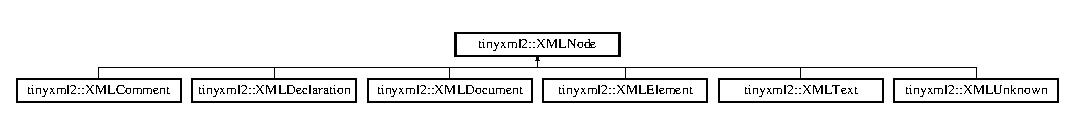
\includegraphics[height=1.145194cm]{classtinyxml2_1_1_x_m_l_node}
\end{center}
\end{figure}
\subsection*{Public Member Functions}
\begin{DoxyCompactItemize}
\item 
const \textbf{ X\+M\+L\+Document} $\ast$ \textbf{ Get\+Document} () const
\begin{DoxyCompactList}\small\item\em Get the \doxyref{X\+M\+L\+Document}{p.}{classtinyxml2_1_1_x_m_l_document} that owns this \doxyref{X\+M\+L\+Node}{p.}{classtinyxml2_1_1_x_m_l_node}. \end{DoxyCompactList}\item 
\textbf{ X\+M\+L\+Document} $\ast$ \textbf{ Get\+Document} ()
\begin{DoxyCompactList}\small\item\em Get the \doxyref{X\+M\+L\+Document}{p.}{classtinyxml2_1_1_x_m_l_document} that owns this \doxyref{X\+M\+L\+Node}{p.}{classtinyxml2_1_1_x_m_l_node}. \end{DoxyCompactList}\item 
virtual \textbf{ X\+M\+L\+Element} $\ast$ \textbf{ To\+Element} ()
\begin{DoxyCompactList}\small\item\em Safely cast to an Element, or null. \end{DoxyCompactList}\item 
virtual \textbf{ X\+M\+L\+Text} $\ast$ \textbf{ To\+Text} ()
\begin{DoxyCompactList}\small\item\em Safely cast to Text, or null. \end{DoxyCompactList}\item 
virtual \textbf{ X\+M\+L\+Comment} $\ast$ \textbf{ To\+Comment} ()
\begin{DoxyCompactList}\small\item\em Safely cast to a Comment, or null. \end{DoxyCompactList}\item 
virtual \textbf{ X\+M\+L\+Document} $\ast$ \textbf{ To\+Document} ()
\begin{DoxyCompactList}\small\item\em Safely cast to a Document, or null. \end{DoxyCompactList}\item 
virtual \textbf{ X\+M\+L\+Declaration} $\ast$ \textbf{ To\+Declaration} ()
\begin{DoxyCompactList}\small\item\em Safely cast to a Declaration, or null. \end{DoxyCompactList}\item 
virtual \textbf{ X\+M\+L\+Unknown} $\ast$ \textbf{ To\+Unknown} ()
\begin{DoxyCompactList}\small\item\em Safely cast to an Unknown, or null. \end{DoxyCompactList}\item 
virtual const \textbf{ X\+M\+L\+Element} $\ast$ \textbf{ To\+Element} () const
\item 
virtual const \textbf{ X\+M\+L\+Text} $\ast$ \textbf{ To\+Text} () const
\item 
virtual const \textbf{ X\+M\+L\+Comment} $\ast$ \textbf{ To\+Comment} () const
\item 
virtual const \textbf{ X\+M\+L\+Document} $\ast$ \textbf{ To\+Document} () const
\item 
virtual const \textbf{ X\+M\+L\+Declaration} $\ast$ \textbf{ To\+Declaration} () const
\item 
virtual const \textbf{ X\+M\+L\+Unknown} $\ast$ \textbf{ To\+Unknown} () const
\item 
const char $\ast$ \textbf{ Value} () const
\item 
void \textbf{ Set\+Value} (const char $\ast$val, bool static\+Mem=false)
\item 
int \textbf{ Get\+Line\+Num} () const
\begin{DoxyCompactList}\small\item\em Gets the line number the node is in, if the document was parsed from a file. \end{DoxyCompactList}\item 
const \textbf{ X\+M\+L\+Node} $\ast$ \textbf{ Parent} () const
\begin{DoxyCompactList}\small\item\em Get the parent of this node on the D\+OM. \end{DoxyCompactList}\item 
\textbf{ X\+M\+L\+Node} $\ast$ \textbf{ Parent} ()
\item 
bool \textbf{ No\+Children} () const
\begin{DoxyCompactList}\small\item\em Returns true if this node has no children. \end{DoxyCompactList}\item 
const \textbf{ X\+M\+L\+Node} $\ast$ \textbf{ First\+Child} () const
\begin{DoxyCompactList}\small\item\em Get the first child node, or null if none exists. \end{DoxyCompactList}\item 
\textbf{ X\+M\+L\+Node} $\ast$ \textbf{ First\+Child} ()
\item 
const \textbf{ X\+M\+L\+Element} $\ast$ \textbf{ First\+Child\+Element} (const char $\ast$name=0) const
\item 
\textbf{ X\+M\+L\+Element} $\ast$ \textbf{ First\+Child\+Element} (const char $\ast$name=0)
\item 
const \textbf{ X\+M\+L\+Node} $\ast$ \textbf{ Last\+Child} () const
\begin{DoxyCompactList}\small\item\em Get the last child node, or null if none exists. \end{DoxyCompactList}\item 
\textbf{ X\+M\+L\+Node} $\ast$ \textbf{ Last\+Child} ()
\item 
const \textbf{ X\+M\+L\+Element} $\ast$ \textbf{ Last\+Child\+Element} (const char $\ast$name=0) const
\item 
\textbf{ X\+M\+L\+Element} $\ast$ \textbf{ Last\+Child\+Element} (const char $\ast$name=0)
\item 
const \textbf{ X\+M\+L\+Node} $\ast$ \textbf{ Previous\+Sibling} () const
\begin{DoxyCompactList}\small\item\em Get the previous (left) sibling node of this node. \end{DoxyCompactList}\item 
\textbf{ X\+M\+L\+Node} $\ast$ \textbf{ Previous\+Sibling} ()
\item 
const \textbf{ X\+M\+L\+Element} $\ast$ \textbf{ Previous\+Sibling\+Element} (const char $\ast$name=0) const
\begin{DoxyCompactList}\small\item\em Get the previous (left) sibling element of this node, with an optionally supplied name. \end{DoxyCompactList}\item 
\textbf{ X\+M\+L\+Element} $\ast$ \textbf{ Previous\+Sibling\+Element} (const char $\ast$name=0)
\item 
const \textbf{ X\+M\+L\+Node} $\ast$ \textbf{ Next\+Sibling} () const
\begin{DoxyCompactList}\small\item\em Get the next (right) sibling node of this node. \end{DoxyCompactList}\item 
\textbf{ X\+M\+L\+Node} $\ast$ \textbf{ Next\+Sibling} ()
\item 
const \textbf{ X\+M\+L\+Element} $\ast$ \textbf{ Next\+Sibling\+Element} (const char $\ast$name=0) const
\begin{DoxyCompactList}\small\item\em Get the next (right) sibling element of this node, with an optionally supplied name. \end{DoxyCompactList}\item 
\textbf{ X\+M\+L\+Element} $\ast$ \textbf{ Next\+Sibling\+Element} (const char $\ast$name=0)
\item 
\textbf{ X\+M\+L\+Node} $\ast$ \textbf{ Insert\+End\+Child} (\textbf{ X\+M\+L\+Node} $\ast$add\+This)
\item 
\textbf{ X\+M\+L\+Node} $\ast$ \textbf{ Link\+End\+Child} (\textbf{ X\+M\+L\+Node} $\ast$add\+This)
\item 
\textbf{ X\+M\+L\+Node} $\ast$ \textbf{ Insert\+First\+Child} (\textbf{ X\+M\+L\+Node} $\ast$add\+This)
\item 
\textbf{ X\+M\+L\+Node} $\ast$ \textbf{ Insert\+After\+Child} (\textbf{ X\+M\+L\+Node} $\ast$after\+This, \textbf{ X\+M\+L\+Node} $\ast$add\+This)
\item 
void \textbf{ Delete\+Children} ()
\item 
void \textbf{ Delete\+Child} (\textbf{ X\+M\+L\+Node} $\ast$node)
\item 
virtual \textbf{ X\+M\+L\+Node} $\ast$ \textbf{ Shallow\+Clone} (\textbf{ X\+M\+L\+Document} $\ast$document) const =0
\item 
\textbf{ X\+M\+L\+Node} $\ast$ \textbf{ Deep\+Clone} (\textbf{ X\+M\+L\+Document} $\ast$target) const
\item 
virtual bool \textbf{ Shallow\+Equal} (const \textbf{ X\+M\+L\+Node} $\ast$compare) const =0
\item 
virtual bool \textbf{ Accept} (\textbf{ X\+M\+L\+Visitor} $\ast$visitor) const =0
\item 
void \textbf{ Set\+User\+Data} (void $\ast$user\+Data)
\item 
void $\ast$ \textbf{ Get\+User\+Data} () const
\end{DoxyCompactItemize}
\subsection*{Protected Member Functions}
\begin{DoxyCompactItemize}
\item 
\textbf{ X\+M\+L\+Node} (\textbf{ X\+M\+L\+Document} $\ast$)
\item 
virtual \textbf{ $\sim$\+X\+M\+L\+Node} ()
\item 
virtual char $\ast$ \textbf{ Parse\+Deep} (char $\ast$p, \textbf{ Str\+Pair} $\ast$parent\+End\+Tag, int $\ast$cur\+Line\+Num\+Ptr)
\end{DoxyCompactItemize}
\subsection*{Protected Attributes}
\begin{DoxyCompactItemize}
\item 
\textbf{ X\+M\+L\+Document} $\ast$ \textbf{ \+\_\+document}
\item 
\textbf{ X\+M\+L\+Node} $\ast$ \textbf{ \+\_\+parent}
\item 
\textbf{ Str\+Pair} \textbf{ \+\_\+value}
\item 
int \textbf{ \+\_\+parse\+Line\+Num}
\item 
\textbf{ X\+M\+L\+Node} $\ast$ \textbf{ \+\_\+first\+Child}
\item 
\textbf{ X\+M\+L\+Node} $\ast$ \textbf{ \+\_\+last\+Child}
\item 
\textbf{ X\+M\+L\+Node} $\ast$ \textbf{ \+\_\+prev}
\item 
\textbf{ X\+M\+L\+Node} $\ast$ \textbf{ \+\_\+next}
\item 
void $\ast$ \textbf{ \+\_\+user\+Data}
\end{DoxyCompactItemize}
\subsection*{Private Member Functions}
\begin{DoxyCompactItemize}
\item 
void \textbf{ Unlink} (\textbf{ X\+M\+L\+Node} $\ast$child)
\item 
void \textbf{ Insert\+Child\+Preamble} (\textbf{ X\+M\+L\+Node} $\ast$insert\+This) const
\item 
const \textbf{ X\+M\+L\+Element} $\ast$ \textbf{ To\+Element\+With\+Name} (const char $\ast$name) const
\item 
\textbf{ X\+M\+L\+Node} (const \textbf{ X\+M\+L\+Node} \&)
\item 
\textbf{ X\+M\+L\+Node} \& \textbf{ operator=} (const \textbf{ X\+M\+L\+Node} \&)
\end{DoxyCompactItemize}
\subsection*{Static Private Member Functions}
\begin{DoxyCompactItemize}
\item 
static void \textbf{ Delete\+Node} (\textbf{ X\+M\+L\+Node} $\ast$node)
\end{DoxyCompactItemize}
\subsection*{Private Attributes}
\begin{DoxyCompactItemize}
\item 
\textbf{ Mem\+Pool} $\ast$ \textbf{ \+\_\+mem\+Pool}
\end{DoxyCompactItemize}
\subsection*{Friends}
\begin{DoxyCompactItemize}
\item 
class \textbf{ X\+M\+L\+Document}
\item 
class \textbf{ X\+M\+L\+Element}
\end{DoxyCompactItemize}


\subsection{Detailed Description}
\doxyref{X\+M\+L\+Node}{p.}{classtinyxml2_1_1_x_m_l_node} is a base class for every object that is in the X\+ML Document Object Model (D\+OM), except X\+M\+L\+Attributes. Nodes have siblings, a parent, and children which can be navigated. A node is always in a \doxyref{X\+M\+L\+Document}{p.}{classtinyxml2_1_1_x_m_l_document}. The type of a \doxyref{X\+M\+L\+Node}{p.}{classtinyxml2_1_1_x_m_l_node} can be queried, and it can be cast to its more defined type.

A \doxyref{X\+M\+L\+Document}{p.}{classtinyxml2_1_1_x_m_l_document} allocates memory for all its Nodes. When the \doxyref{X\+M\+L\+Document}{p.}{classtinyxml2_1_1_x_m_l_document} gets deleted, all its Nodes will also be deleted.

\begin{DoxyVerb}A Document can contain: Element (container or leaf)
                        Comment (leaf)
                        Unknown (leaf)
                        Declaration( leaf )

An Element can contain: Element (container or leaf)
                        Text    (leaf)
                        Attributes (not on tree)
                        Comment (leaf)
                        Unknown (leaf)\end{DoxyVerb}
 

Definition at line 667 of file tinyxml2.\+h.



\subsection{Constructor \& Destructor Documentation}
\mbox{\label{classtinyxml2_1_1_x_m_l_node_a29868df6ca383d574f584dfdd15105b6}} 
\index{tinyxml2::XMLNode@{tinyxml2::XMLNode}!XMLNode@{XMLNode}}
\index{XMLNode@{XMLNode}!tinyxml2::XMLNode@{tinyxml2::XMLNode}}
\subsubsection{XMLNode()\hspace{0.1cm}{\footnotesize\ttfamily [1/2]}}
{\footnotesize\ttfamily tinyxml2\+::\+X\+M\+L\+Node\+::\+X\+M\+L\+Node (\begin{DoxyParamCaption}\item[{\textbf{ X\+M\+L\+Document} $\ast$}]{doc }\end{DoxyParamCaption})\hspace{0.3cm}{\ttfamily [explicit]}, {\ttfamily [protected]}}



Definition at line 742 of file tinyxml2.\+cpp.

\mbox{\label{classtinyxml2_1_1_x_m_l_node_a8f41e898cdd4da4cdbb7f05b0c7d9f69}} 
\index{tinyxml2::XMLNode@{tinyxml2::XMLNode}!````~XMLNode@{$\sim$XMLNode}}
\index{````~XMLNode@{$\sim$XMLNode}!tinyxml2::XMLNode@{tinyxml2::XMLNode}}
\subsubsection{$\sim$XMLNode()}
{\footnotesize\ttfamily tinyxml2\+::\+X\+M\+L\+Node\+::$\sim$\+X\+M\+L\+Node (\begin{DoxyParamCaption}{ }\end{DoxyParamCaption})\hspace{0.3cm}{\ttfamily [protected]}, {\ttfamily [virtual]}}



Definition at line 755 of file tinyxml2.\+cpp.



References \+\_\+parent, Delete\+Children(), and Unlink().



Referenced by Delete\+Node().

\mbox{\label{classtinyxml2_1_1_x_m_l_node_a78be01384518a969da905548f318d75b}} 
\index{tinyxml2::XMLNode@{tinyxml2::XMLNode}!XMLNode@{XMLNode}}
\index{XMLNode@{XMLNode}!tinyxml2::XMLNode@{tinyxml2::XMLNode}}
\subsubsection{XMLNode()\hspace{0.1cm}{\footnotesize\ttfamily [2/2]}}
{\footnotesize\ttfamily tinyxml2\+::\+X\+M\+L\+Node\+::\+X\+M\+L\+Node (\begin{DoxyParamCaption}\item[{const \textbf{ X\+M\+L\+Node} \&}]{ }\end{DoxyParamCaption})\hspace{0.3cm}{\ttfamily [private]}}



\subsection{Member Function Documentation}
\mbox{\label{classtinyxml2_1_1_x_m_l_node_a81e66df0a44c67a7af17f3b77a152785}} 
\index{tinyxml2::XMLNode@{tinyxml2::XMLNode}!Accept@{Accept}}
\index{Accept@{Accept}!tinyxml2::XMLNode@{tinyxml2::XMLNode}}
\subsubsection{Accept()}
{\footnotesize\ttfamily virtual bool tinyxml2\+::\+X\+M\+L\+Node\+::\+Accept (\begin{DoxyParamCaption}\item[{\textbf{ X\+M\+L\+Visitor} $\ast$}]{visitor }\end{DoxyParamCaption}) const\hspace{0.3cm}{\ttfamily [pure virtual]}}

Accept a hierarchical visit of the nodes in the Tiny\+X\+M\+L-\/2 D\+OM. Every node in the X\+ML tree will be conditionally visited and the host will be called back via the \doxyref{X\+M\+L\+Visitor}{p.}{classtinyxml2_1_1_x_m_l_visitor} interface.

This is essentially a S\+AX interface for Tiny\+X\+M\+L-\/2. (Note however it doesn\textquotesingle{}t re-\/parse the X\+ML for the callbacks, so the performance of Tiny\+X\+M\+L-\/2 is unchanged by using this interface versus any other.)

The interface has been based on ideas from\+:


\begin{DoxyItemize}
\item {\texttt{ http\+://www.\+saxproject.\+org/}}
\item {\texttt{ http\+://c2.\+com/cgi/wiki?\+Hierarchical\+Visitor\+Pattern}}
\end{DoxyItemize}

Which are both good references for \char`\"{}visiting\char`\"{}.

An example of using \doxyref{Accept()}{p.}{classtinyxml2_1_1_x_m_l_node_a81e66df0a44c67a7af17f3b77a152785}\+: \begin{DoxyVerb}XMLPrinter printer;
tinyxmlDoc.Accept( &printer );
const char* xmlcstr = printer.CStr();
\end{DoxyVerb}
 

Implemented in \textbf{ tinyxml2\+::\+X\+M\+L\+Document} \doxyref{}{p.}{classtinyxml2_1_1_x_m_l_document_ab7be651917a35ab1ff0e4e6d4e565cdf}, \textbf{ tinyxml2\+::\+X\+M\+L\+Element} \doxyref{}{p.}{classtinyxml2_1_1_x_m_l_element_a9b2119831e8b85827d5d3e5076788e4a}, \textbf{ tinyxml2\+::\+X\+M\+L\+Unknown} \doxyref{}{p.}{classtinyxml2_1_1_x_m_l_unknown_a8a06b8c82117ca969a432e17a46830fc}, \textbf{ tinyxml2\+::\+X\+M\+L\+Declaration} \doxyref{}{p.}{classtinyxml2_1_1_x_m_l_declaration_acf47629d9fc08ed6f1c164a97bcf794b}, \textbf{ tinyxml2\+::\+X\+M\+L\+Comment} \doxyref{}{p.}{classtinyxml2_1_1_x_m_l_comment_a27b37d16cea01b5329dfbbb4f9508e39}, and \textbf{ tinyxml2\+::\+X\+M\+L\+Text} \doxyref{}{p.}{classtinyxml2_1_1_x_m_l_text_a537c60d7e18fb59c45ac2737a29ac47a}.

\mbox{\label{classtinyxml2_1_1_x_m_l_node_a3bb369fd733f1989b751d99a9417adab}} 
\index{tinyxml2::XMLNode@{tinyxml2::XMLNode}!DeepClone@{DeepClone}}
\index{DeepClone@{DeepClone}!tinyxml2::XMLNode@{tinyxml2::XMLNode}}
\subsubsection{DeepClone()}
{\footnotesize\ttfamily \textbf{ X\+M\+L\+Node} $\ast$ tinyxml2\+::\+X\+M\+L\+Node\+::\+Deep\+Clone (\begin{DoxyParamCaption}\item[{\textbf{ X\+M\+L\+Document} $\ast$}]{target }\end{DoxyParamCaption}) const}

Make a copy of this node and all its children.

If the \textquotesingle{}target\textquotesingle{} is null, then the nodes will be allocated in the current document. If \textquotesingle{}target\textquotesingle{} is specified, the memory will be allocated is the specified \doxyref{X\+M\+L\+Document}{p.}{classtinyxml2_1_1_x_m_l_document}.

N\+O\+TE\+: This is probably not the correct tool to copy a document, since X\+M\+L\+Documents can have multiple top level X\+M\+L\+Nodes. You probably want to use \doxyref{X\+M\+L\+Document\+::\+Deep\+Copy()}{p.}{classtinyxml2_1_1_x_m_l_document_af592ffc91514e25a39664521ac83db45} 

Definition at line 781 of file tinyxml2.\+cpp.



References Deep\+Clone(), First\+Child(), Insert\+End\+Child(), Next\+Sibling(), Shallow\+Clone(), and T\+I\+X\+M\+L\+A\+S\+S\+E\+RT.



Referenced by Deep\+Clone().

\mbox{\label{classtinyxml2_1_1_x_m_l_node_a363b6edbd6ebd55f8387d2b89f2b0921}} 
\index{tinyxml2::XMLNode@{tinyxml2::XMLNode}!DeleteChild@{DeleteChild}}
\index{DeleteChild@{DeleteChild}!tinyxml2::XMLNode@{tinyxml2::XMLNode}}
\subsubsection{DeleteChild()}
{\footnotesize\ttfamily void tinyxml2\+::\+X\+M\+L\+Node\+::\+Delete\+Child (\begin{DoxyParamCaption}\item[{\textbf{ X\+M\+L\+Node} $\ast$}]{node }\end{DoxyParamCaption})}

Delete a child of this node. 

Definition at line 828 of file tinyxml2.\+cpp.



References \+\_\+document, \+\_\+next, \+\_\+parent, \+\_\+prev, Delete\+Node(), T\+I\+X\+M\+L\+A\+S\+S\+E\+RT, and Unlink().



Referenced by Delete\+Children(), and tinyxml2\+::\+X\+M\+L\+Document\+::\+Delete\+Node().

\mbox{\label{classtinyxml2_1_1_x_m_l_node_a0360085cc54df5bff85d5c5da13afdce}} 
\index{tinyxml2::XMLNode@{tinyxml2::XMLNode}!DeleteChildren@{DeleteChildren}}
\index{DeleteChildren@{DeleteChildren}!tinyxml2::XMLNode@{tinyxml2::XMLNode}}
\subsubsection{DeleteChildren()}
{\footnotesize\ttfamily void tinyxml2\+::\+X\+M\+L\+Node\+::\+Delete\+Children (\begin{DoxyParamCaption}{ }\end{DoxyParamCaption})}

Delete all the children of this node. 

Definition at line 794 of file tinyxml2.\+cpp.



References \+\_\+first\+Child, \+\_\+last\+Child, Delete\+Child(), and T\+I\+X\+M\+L\+A\+S\+S\+E\+RT.



Referenced by tinyxml2\+::\+X\+M\+L\+Document\+::\+Clear(), tinyxml2\+::\+X\+M\+L\+Document\+::\+Parse(), and $\sim$\+X\+M\+L\+Node().

\mbox{\label{classtinyxml2_1_1_x_m_l_node_ab0b21951f2343534c5c67f23dffdc7e6}} 
\index{tinyxml2::XMLNode@{tinyxml2::XMLNode}!DeleteNode@{DeleteNode}}
\index{DeleteNode@{DeleteNode}!tinyxml2::XMLNode@{tinyxml2::XMLNode}}
\subsubsection{DeleteNode()}
{\footnotesize\ttfamily void tinyxml2\+::\+X\+M\+L\+Node\+::\+Delete\+Node (\begin{DoxyParamCaption}\item[{\textbf{ X\+M\+L\+Node} $\ast$}]{node }\end{DoxyParamCaption})\hspace{0.3cm}{\ttfamily [static]}, {\ttfamily [private]}}



Definition at line 1102 of file tinyxml2.\+cpp.



References \+\_\+document, \+\_\+mem\+Pool, tinyxml2\+::\+Mem\+Pool\+::\+Free(), tinyxml2\+::\+X\+M\+L\+Document\+::\+Mark\+In\+Use(), T\+I\+X\+M\+L\+A\+S\+S\+E\+RT, To\+Document(), and $\sim$\+X\+M\+L\+Node().



Referenced by Delete\+Child(), tinyxml2\+::\+X\+M\+L\+Document\+::\+Delete\+Node(), and Parse\+Deep().

\mbox{\label{classtinyxml2_1_1_x_m_l_node_ae7dc225e1018cdd685f7563593a1fe08}} 
\index{tinyxml2::XMLNode@{tinyxml2::XMLNode}!FirstChild@{FirstChild}}
\index{FirstChild@{FirstChild}!tinyxml2::XMLNode@{tinyxml2::XMLNode}}
\subsubsection{FirstChild()\hspace{0.1cm}{\footnotesize\ttfamily [1/2]}}
{\footnotesize\ttfamily const \textbf{ X\+M\+L\+Node}$\ast$ tinyxml2\+::\+X\+M\+L\+Node\+::\+First\+Child (\begin{DoxyParamCaption}{ }\end{DoxyParamCaption}) const\hspace{0.3cm}{\ttfamily [inline]}}



Get the first child node, or null if none exists. 



Definition at line 762 of file tinyxml2.\+h.



Referenced by tinyxml2\+::\+X\+M\+L\+Element\+::\+Accept(), tinyxml2\+::\+X\+M\+L\+Document\+::\+Accept(), Deep\+Clone(), tinyxml2\+::\+X\+M\+L\+Document\+::\+Deep\+Copy(), utils\+::get\+Node(), tinyxml2\+::\+X\+M\+L\+Element\+::\+Get\+Text(), Parse\+Deep(), tinyxml2\+::\+X\+M\+L\+Element\+::\+Query\+Bool\+Text(), tinyxml2\+::\+X\+M\+L\+Element\+::\+Query\+Double\+Text(), tinyxml2\+::\+X\+M\+L\+Element\+::\+Query\+Float\+Text(), tinyxml2\+::\+X\+M\+L\+Element\+::\+Query\+Int64\+Text(), tinyxml2\+::\+X\+M\+L\+Element\+::\+Query\+Int\+Text(), tinyxml2\+::\+X\+M\+L\+Element\+::\+Query\+Unsigned\+Text(), and tinyxml2\+::\+X\+M\+L\+Element\+::\+Set\+Text().

\mbox{\label{classtinyxml2_1_1_x_m_l_node_a2d6c70c475146b48bc93a7fafdeff5e0}} 
\index{tinyxml2::XMLNode@{tinyxml2::XMLNode}!FirstChild@{FirstChild}}
\index{FirstChild@{FirstChild}!tinyxml2::XMLNode@{tinyxml2::XMLNode}}
\subsubsection{FirstChild()\hspace{0.1cm}{\footnotesize\ttfamily [2/2]}}
{\footnotesize\ttfamily \textbf{ X\+M\+L\+Node}$\ast$ tinyxml2\+::\+X\+M\+L\+Node\+::\+First\+Child (\begin{DoxyParamCaption}{ }\end{DoxyParamCaption})\hspace{0.3cm}{\ttfamily [inline]}}



Definition at line 766 of file tinyxml2.\+h.

\mbox{\label{classtinyxml2_1_1_x_m_l_node_a1bec132dcf085284e0a10755f2cf0d57}} 
\index{tinyxml2::XMLNode@{tinyxml2::XMLNode}!FirstChildElement@{FirstChildElement}}
\index{FirstChildElement@{FirstChildElement}!tinyxml2::XMLNode@{tinyxml2::XMLNode}}
\subsubsection{FirstChildElement()\hspace{0.1cm}{\footnotesize\ttfamily [1/2]}}
{\footnotesize\ttfamily const \textbf{ X\+M\+L\+Element} $\ast$ tinyxml2\+::\+X\+M\+L\+Node\+::\+First\+Child\+Element (\begin{DoxyParamCaption}\item[{const char $\ast$}]{name = {\ttfamily 0} }\end{DoxyParamCaption}) const}

Get the first child element, or optionally the first child element with the specified name. 

Definition at line 940 of file tinyxml2.\+cpp.



References \+\_\+first\+Child, and \+\_\+next.



Referenced by utils\+::get\+First\+Child\+Element(), utils\+::get\+Node(), World\+::parse\+Antennas(), World\+::parse\+Persons(), and World\+::parse\+Simulation\+File().

\mbox{\label{classtinyxml2_1_1_x_m_l_node_af1e0e475cc27d5e7eeaf4d732691b741}} 
\index{tinyxml2::XMLNode@{tinyxml2::XMLNode}!FirstChildElement@{FirstChildElement}}
\index{FirstChildElement@{FirstChildElement}!tinyxml2::XMLNode@{tinyxml2::XMLNode}}
\subsubsection{FirstChildElement()\hspace{0.1cm}{\footnotesize\ttfamily [2/2]}}
{\footnotesize\ttfamily \textbf{ X\+M\+L\+Element}$\ast$ tinyxml2\+::\+X\+M\+L\+Node\+::\+First\+Child\+Element (\begin{DoxyParamCaption}\item[{const char $\ast$}]{name = {\ttfamily 0} }\end{DoxyParamCaption})\hspace{0.3cm}{\ttfamily [inline]}}



Definition at line 775 of file tinyxml2.\+h.

\mbox{\label{classtinyxml2_1_1_x_m_l_node_a2de84cfa4ec3fe249bad745069d145f1}} 
\index{tinyxml2::XMLNode@{tinyxml2::XMLNode}!GetDocument@{GetDocument}}
\index{GetDocument@{GetDocument}!tinyxml2::XMLNode@{tinyxml2::XMLNode}}
\subsubsection{GetDocument()\hspace{0.1cm}{\footnotesize\ttfamily [1/2]}}
{\footnotesize\ttfamily const \textbf{ X\+M\+L\+Document}$\ast$ tinyxml2\+::\+X\+M\+L\+Node\+::\+Get\+Document (\begin{DoxyParamCaption}{ }\end{DoxyParamCaption}) const\hspace{0.3cm}{\ttfamily [inline]}}



Get the \doxyref{X\+M\+L\+Document}{p.}{classtinyxml2_1_1_x_m_l_document} that owns this \doxyref{X\+M\+L\+Node}{p.}{classtinyxml2_1_1_x_m_l_node}. 



Definition at line 674 of file tinyxml2.\+h.



References T\+I\+X\+M\+L\+A\+S\+S\+E\+RT.



Referenced by tinyxml2\+::\+X\+M\+L\+Element\+::\+Set\+Text().

\mbox{\label{classtinyxml2_1_1_x_m_l_node_af343d1ef0b45c0020e62d784d7e67a68}} 
\index{tinyxml2::XMLNode@{tinyxml2::XMLNode}!GetDocument@{GetDocument}}
\index{GetDocument@{GetDocument}!tinyxml2::XMLNode@{tinyxml2::XMLNode}}
\subsubsection{GetDocument()\hspace{0.1cm}{\footnotesize\ttfamily [2/2]}}
{\footnotesize\ttfamily \textbf{ X\+M\+L\+Document}$\ast$ tinyxml2\+::\+X\+M\+L\+Node\+::\+Get\+Document (\begin{DoxyParamCaption}{ }\end{DoxyParamCaption})\hspace{0.3cm}{\ttfamily [inline]}}



Get the \doxyref{X\+M\+L\+Document}{p.}{classtinyxml2_1_1_x_m_l_document} that owns this \doxyref{X\+M\+L\+Node}{p.}{classtinyxml2_1_1_x_m_l_node}. 



Definition at line 679 of file tinyxml2.\+h.



References T\+I\+X\+M\+L\+A\+S\+S\+E\+RT.

\mbox{\label{classtinyxml2_1_1_x_m_l_node_a9b5fc636646fda761d342c72e91cb286}} 
\index{tinyxml2::XMLNode@{tinyxml2::XMLNode}!GetLineNum@{GetLineNum}}
\index{GetLineNum@{GetLineNum}!tinyxml2::XMLNode@{tinyxml2::XMLNode}}
\subsubsection{GetLineNum()}
{\footnotesize\ttfamily int tinyxml2\+::\+X\+M\+L\+Node\+::\+Get\+Line\+Num (\begin{DoxyParamCaption}{ }\end{DoxyParamCaption}) const\hspace{0.3cm}{\ttfamily [inline]}}



Gets the line number the node is in, if the document was parsed from a file. 



Definition at line 745 of file tinyxml2.\+h.

\mbox{\label{classtinyxml2_1_1_x_m_l_node_a7f0687574afa03bc479dc44f29db0afe}} 
\index{tinyxml2::XMLNode@{tinyxml2::XMLNode}!GetUserData@{GetUserData}}
\index{GetUserData@{GetUserData}!tinyxml2::XMLNode@{tinyxml2::XMLNode}}
\subsubsection{GetUserData()}
{\footnotesize\ttfamily void$\ast$ tinyxml2\+::\+X\+M\+L\+Node\+::\+Get\+User\+Data (\begin{DoxyParamCaption}{ }\end{DoxyParamCaption}) const\hspace{0.3cm}{\ttfamily [inline]}}

Get user data set into the \doxyref{X\+M\+L\+Node}{p.}{classtinyxml2_1_1_x_m_l_node}. Tiny\+X\+M\+L-\/2 in no way processes or interprets user data. It is initially 0. 

Definition at line 939 of file tinyxml2.\+h.

\mbox{\label{classtinyxml2_1_1_x_m_l_node_a9275138a1b8dd5d8e2c26789bdc23ac8}} 
\index{tinyxml2::XMLNode@{tinyxml2::XMLNode}!InsertAfterChild@{InsertAfterChild}}
\index{InsertAfterChild@{InsertAfterChild}!tinyxml2::XMLNode@{tinyxml2::XMLNode}}
\subsubsection{InsertAfterChild()}
{\footnotesize\ttfamily \textbf{ X\+M\+L\+Node} $\ast$ tinyxml2\+::\+X\+M\+L\+Node\+::\+Insert\+After\+Child (\begin{DoxyParamCaption}\item[{\textbf{ X\+M\+L\+Node} $\ast$}]{after\+This,  }\item[{\textbf{ X\+M\+L\+Node} $\ast$}]{add\+This }\end{DoxyParamCaption})}

Add a node after the specified child node. If the child node is already part of the document, it is moved from its old location to the new location. Returns the add\+This argument or 0 if the after\+This node is not a child of this node, or if the node does not belong to the same document. 

Definition at line 902 of file tinyxml2.\+cpp.



References \+\_\+document, \+\_\+next, \+\_\+parent, \+\_\+prev, Insert\+Child\+Preamble(), Insert\+End\+Child(), and T\+I\+X\+M\+L\+A\+S\+S\+E\+RT.

\mbox{\label{classtinyxml2_1_1_x_m_l_node_a0fd4d2e88fb22d46b5b1474b5b786e35}} 
\index{tinyxml2::XMLNode@{tinyxml2::XMLNode}!InsertChildPreamble@{InsertChildPreamble}}
\index{InsertChildPreamble@{InsertChildPreamble}!tinyxml2::XMLNode@{tinyxml2::XMLNode}}
\subsubsection{InsertChildPreamble()}
{\footnotesize\ttfamily void tinyxml2\+::\+X\+M\+L\+Node\+::\+Insert\+Child\+Preamble (\begin{DoxyParamCaption}\item[{\textbf{ X\+M\+L\+Node} $\ast$}]{insert\+This }\end{DoxyParamCaption}) const\hspace{0.3cm}{\ttfamily [private]}}



Definition at line 1117 of file tinyxml2.\+cpp.



References \+\_\+document, \+\_\+mem\+Pool, \+\_\+parent, tinyxml2\+::\+X\+M\+L\+Document\+::\+Mark\+In\+Use(), tinyxml2\+::\+Mem\+Pool\+::\+Set\+Tracked(), T\+I\+X\+M\+L\+A\+S\+S\+E\+RT, and Unlink().



Referenced by Insert\+After\+Child(), Insert\+End\+Child(), and Insert\+First\+Child().

\mbox{\label{classtinyxml2_1_1_x_m_l_node_ae3b422e98914d6002ca99bb1d2837103}} 
\index{tinyxml2::XMLNode@{tinyxml2::XMLNode}!InsertEndChild@{InsertEndChild}}
\index{InsertEndChild@{InsertEndChild}!tinyxml2::XMLNode@{tinyxml2::XMLNode}}
\subsubsection{InsertEndChild()}
{\footnotesize\ttfamily \textbf{ X\+M\+L\+Node} $\ast$ tinyxml2\+::\+X\+M\+L\+Node\+::\+Insert\+End\+Child (\begin{DoxyParamCaption}\item[{\textbf{ X\+M\+L\+Node} $\ast$}]{add\+This }\end{DoxyParamCaption})}

Add a child node as the last (right) child. If the child node is already part of the document, it is moved from its old location to the new location. Returns the add\+This argument or 0 if the node does not belong to the same document. 

Definition at line 841 of file tinyxml2.\+cpp.



References \+\_\+document, \+\_\+first\+Child, \+\_\+last\+Child, \+\_\+next, \+\_\+parent, \+\_\+prev, Insert\+Child\+Preamble(), and T\+I\+X\+M\+L\+A\+S\+S\+E\+RT.



Referenced by Deep\+Clone(), tinyxml2\+::\+X\+M\+L\+Document\+::\+Deep\+Copy(), Insert\+After\+Child(), and Parse\+Deep().

\mbox{\label{classtinyxml2_1_1_x_m_l_node_ac609a8f3ea949027f439280c640bbaf2}} 
\index{tinyxml2::XMLNode@{tinyxml2::XMLNode}!InsertFirstChild@{InsertFirstChild}}
\index{InsertFirstChild@{InsertFirstChild}!tinyxml2::XMLNode@{tinyxml2::XMLNode}}
\subsubsection{InsertFirstChild()}
{\footnotesize\ttfamily \textbf{ X\+M\+L\+Node} $\ast$ tinyxml2\+::\+X\+M\+L\+Node\+::\+Insert\+First\+Child (\begin{DoxyParamCaption}\item[{\textbf{ X\+M\+L\+Node} $\ast$}]{add\+This }\end{DoxyParamCaption})}

Add a child node as the first (left) child. If the child node is already part of the document, it is moved from its old location to the new location. Returns the add\+This argument or 0 if the node does not belong to the same document. 

Definition at line 871 of file tinyxml2.\+cpp.



References \+\_\+document, \+\_\+first\+Child, \+\_\+last\+Child, \+\_\+next, \+\_\+parent, \+\_\+prev, Insert\+Child\+Preamble(), and T\+I\+X\+M\+L\+A\+S\+S\+E\+RT.



Referenced by tinyxml2\+::\+X\+M\+L\+Element\+::\+Set\+Text().

\mbox{\label{classtinyxml2_1_1_x_m_l_node_a9b8583a277e8e26f4cbbb5492786778e}} 
\index{tinyxml2::XMLNode@{tinyxml2::XMLNode}!LastChild@{LastChild}}
\index{LastChild@{LastChild}!tinyxml2::XMLNode@{tinyxml2::XMLNode}}
\subsubsection{LastChild()\hspace{0.1cm}{\footnotesize\ttfamily [1/2]}}
{\footnotesize\ttfamily const \textbf{ X\+M\+L\+Node}$\ast$ tinyxml2\+::\+X\+M\+L\+Node\+::\+Last\+Child (\begin{DoxyParamCaption}{ }\end{DoxyParamCaption}) const\hspace{0.3cm}{\ttfamily [inline]}}



Get the last child node, or null if none exists. 



Definition at line 780 of file tinyxml2.\+h.



Referenced by Parse\+Deep().

\mbox{\label{classtinyxml2_1_1_x_m_l_node_ad7552c8cb1dc0cb6f3bdc14a9d115dbf}} 
\index{tinyxml2::XMLNode@{tinyxml2::XMLNode}!LastChild@{LastChild}}
\index{LastChild@{LastChild}!tinyxml2::XMLNode@{tinyxml2::XMLNode}}
\subsubsection{LastChild()\hspace{0.1cm}{\footnotesize\ttfamily [2/2]}}
{\footnotesize\ttfamily \textbf{ X\+M\+L\+Node}$\ast$ tinyxml2\+::\+X\+M\+L\+Node\+::\+Last\+Child (\begin{DoxyParamCaption}{ }\end{DoxyParamCaption})\hspace{0.3cm}{\ttfamily [inline]}}



Definition at line 784 of file tinyxml2.\+h.

\mbox{\label{classtinyxml2_1_1_x_m_l_node_a609e02f02044f39b928d1a3e0de9f532}} 
\index{tinyxml2::XMLNode@{tinyxml2::XMLNode}!LastChildElement@{LastChildElement}}
\index{LastChildElement@{LastChildElement}!tinyxml2::XMLNode@{tinyxml2::XMLNode}}
\subsubsection{LastChildElement()\hspace{0.1cm}{\footnotesize\ttfamily [1/2]}}
{\footnotesize\ttfamily const \textbf{ X\+M\+L\+Element} $\ast$ tinyxml2\+::\+X\+M\+L\+Node\+::\+Last\+Child\+Element (\begin{DoxyParamCaption}\item[{const char $\ast$}]{name = {\ttfamily 0} }\end{DoxyParamCaption}) const}

Get the last child element or optionally the last child element with the specified name. 

Definition at line 952 of file tinyxml2.\+cpp.



References \+\_\+last\+Child, and \+\_\+prev.

\mbox{\label{classtinyxml2_1_1_x_m_l_node_a1b77a8194d059665a4412ebfea276878}} 
\index{tinyxml2::XMLNode@{tinyxml2::XMLNode}!LastChildElement@{LastChildElement}}
\index{LastChildElement@{LastChildElement}!tinyxml2::XMLNode@{tinyxml2::XMLNode}}
\subsubsection{LastChildElement()\hspace{0.1cm}{\footnotesize\ttfamily [2/2]}}
{\footnotesize\ttfamily \textbf{ X\+M\+L\+Element}$\ast$ tinyxml2\+::\+X\+M\+L\+Node\+::\+Last\+Child\+Element (\begin{DoxyParamCaption}\item[{const char $\ast$}]{name = {\ttfamily 0} }\end{DoxyParamCaption})\hspace{0.3cm}{\ttfamily [inline]}}



Definition at line 793 of file tinyxml2.\+h.

\mbox{\label{classtinyxml2_1_1_x_m_l_node_a663e3a5a378169fd477378f4d17a7649}} 
\index{tinyxml2::XMLNode@{tinyxml2::XMLNode}!LinkEndChild@{LinkEndChild}}
\index{LinkEndChild@{LinkEndChild}!tinyxml2::XMLNode@{tinyxml2::XMLNode}}
\subsubsection{LinkEndChild()}
{\footnotesize\ttfamily \textbf{ X\+M\+L\+Node}$\ast$ tinyxml2\+::\+X\+M\+L\+Node\+::\+Link\+End\+Child (\begin{DoxyParamCaption}\item[{\textbf{ X\+M\+L\+Node} $\ast$}]{add\+This }\end{DoxyParamCaption})\hspace{0.3cm}{\ttfamily [inline]}}



Definition at line 838 of file tinyxml2.\+h.

\mbox{\label{classtinyxml2_1_1_x_m_l_node_a79db9ef0fe014d27790f2218b87bcbb5}} 
\index{tinyxml2::XMLNode@{tinyxml2::XMLNode}!NextSibling@{NextSibling}}
\index{NextSibling@{NextSibling}!tinyxml2::XMLNode@{tinyxml2::XMLNode}}
\subsubsection{NextSibling()\hspace{0.1cm}{\footnotesize\ttfamily [1/2]}}
{\footnotesize\ttfamily const \textbf{ X\+M\+L\+Node}$\ast$ tinyxml2\+::\+X\+M\+L\+Node\+::\+Next\+Sibling (\begin{DoxyParamCaption}{ }\end{DoxyParamCaption}) const\hspace{0.3cm}{\ttfamily [inline]}}



Get the next (right) sibling node of this node. 



Definition at line 814 of file tinyxml2.\+h.



Referenced by tinyxml2\+::\+X\+M\+L\+Element\+::\+Accept(), tinyxml2\+::\+X\+M\+L\+Document\+::\+Accept(), Deep\+Clone(), and tinyxml2\+::\+X\+M\+L\+Document\+::\+Deep\+Copy().

\mbox{\label{classtinyxml2_1_1_x_m_l_node_aeb7d4dfd8fb924ef86e7cb72183acbac}} 
\index{tinyxml2::XMLNode@{tinyxml2::XMLNode}!NextSibling@{NextSibling}}
\index{NextSibling@{NextSibling}!tinyxml2::XMLNode@{tinyxml2::XMLNode}}
\subsubsection{NextSibling()\hspace{0.1cm}{\footnotesize\ttfamily [2/2]}}
{\footnotesize\ttfamily \textbf{ X\+M\+L\+Node}$\ast$ tinyxml2\+::\+X\+M\+L\+Node\+::\+Next\+Sibling (\begin{DoxyParamCaption}{ }\end{DoxyParamCaption})\hspace{0.3cm}{\ttfamily [inline]}}



Definition at line 818 of file tinyxml2.\+h.

\mbox{\label{classtinyxml2_1_1_x_m_l_node_a14ea560df31110ff07a9f566171bf797}} 
\index{tinyxml2::XMLNode@{tinyxml2::XMLNode}!NextSiblingElement@{NextSiblingElement}}
\index{NextSiblingElement@{NextSiblingElement}!tinyxml2::XMLNode@{tinyxml2::XMLNode}}
\subsubsection{NextSiblingElement()\hspace{0.1cm}{\footnotesize\ttfamily [1/2]}}
{\footnotesize\ttfamily const \textbf{ X\+M\+L\+Element} $\ast$ tinyxml2\+::\+X\+M\+L\+Node\+::\+Next\+Sibling\+Element (\begin{DoxyParamCaption}\item[{const char $\ast$}]{name = {\ttfamily 0} }\end{DoxyParamCaption}) const}



Get the next (right) sibling element of this node, with an optionally supplied name. 



Definition at line 964 of file tinyxml2.\+cpp.



References \+\_\+next.



Referenced by World\+::parse\+Antennas().

\mbox{\label{classtinyxml2_1_1_x_m_l_node_af1225412584d4a2126f55e96a12e0ec0}} 
\index{tinyxml2::XMLNode@{tinyxml2::XMLNode}!NextSiblingElement@{NextSiblingElement}}
\index{NextSiblingElement@{NextSiblingElement}!tinyxml2::XMLNode@{tinyxml2::XMLNode}}
\subsubsection{NextSiblingElement()\hspace{0.1cm}{\footnotesize\ttfamily [2/2]}}
{\footnotesize\ttfamily \textbf{ X\+M\+L\+Element}$\ast$ tinyxml2\+::\+X\+M\+L\+Node\+::\+Next\+Sibling\+Element (\begin{DoxyParamCaption}\item[{const char $\ast$}]{name = {\ttfamily 0} }\end{DoxyParamCaption})\hspace{0.3cm}{\ttfamily [inline]}}



Definition at line 825 of file tinyxml2.\+h.

\mbox{\label{classtinyxml2_1_1_x_m_l_node_ac3ab489e6e202a3cd1762d3b332e89d4}} 
\index{tinyxml2::XMLNode@{tinyxml2::XMLNode}!NoChildren@{NoChildren}}
\index{NoChildren@{NoChildren}!tinyxml2::XMLNode@{tinyxml2::XMLNode}}
\subsubsection{NoChildren()}
{\footnotesize\ttfamily bool tinyxml2\+::\+X\+M\+L\+Node\+::\+No\+Children (\begin{DoxyParamCaption}{ }\end{DoxyParamCaption}) const\hspace{0.3cm}{\ttfamily [inline]}}



Returns true if this node has no children. 



Definition at line 757 of file tinyxml2.\+h.



Referenced by tinyxml2\+::\+X\+M\+L\+Document\+::\+Parse().

\mbox{\label{classtinyxml2_1_1_x_m_l_node_ade79231d908e1f21862819e00e56ab6e}} 
\index{tinyxml2::XMLNode@{tinyxml2::XMLNode}!operator=@{operator=}}
\index{operator=@{operator=}!tinyxml2::XMLNode@{tinyxml2::XMLNode}}
\subsubsection{operator=()}
{\footnotesize\ttfamily \textbf{ X\+M\+L\+Node}\& tinyxml2\+::\+X\+M\+L\+Node\+::operator= (\begin{DoxyParamCaption}\item[{const \textbf{ X\+M\+L\+Node} \&}]{ }\end{DoxyParamCaption})\hspace{0.3cm}{\ttfamily [private]}}

\mbox{\label{classtinyxml2_1_1_x_m_l_node_ae0f62bc186c56c2e0483ebd52dbfbe34}} 
\index{tinyxml2::XMLNode@{tinyxml2::XMLNode}!Parent@{Parent}}
\index{Parent@{Parent}!tinyxml2::XMLNode@{tinyxml2::XMLNode}}
\subsubsection{Parent()\hspace{0.1cm}{\footnotesize\ttfamily [1/2]}}
{\footnotesize\ttfamily const \textbf{ X\+M\+L\+Node}$\ast$ tinyxml2\+::\+X\+M\+L\+Node\+::\+Parent (\begin{DoxyParamCaption}{ }\end{DoxyParamCaption}) const\hspace{0.3cm}{\ttfamily [inline]}}



Get the parent of this node on the D\+OM. 



Definition at line 748 of file tinyxml2.\+h.



Referenced by tinyxml2\+::\+X\+M\+L\+Printer\+::\+Visit\+Enter().

\mbox{\label{classtinyxml2_1_1_x_m_l_node_a76029693a5a54fbb721a41d7a0ca8a97}} 
\index{tinyxml2::XMLNode@{tinyxml2::XMLNode}!Parent@{Parent}}
\index{Parent@{Parent}!tinyxml2::XMLNode@{tinyxml2::XMLNode}}
\subsubsection{Parent()\hspace{0.1cm}{\footnotesize\ttfamily [2/2]}}
{\footnotesize\ttfamily \textbf{ X\+M\+L\+Node}$\ast$ tinyxml2\+::\+X\+M\+L\+Node\+::\+Parent (\begin{DoxyParamCaption}{ }\end{DoxyParamCaption})\hspace{0.3cm}{\ttfamily [inline]}}



Definition at line 752 of file tinyxml2.\+h.

\mbox{\label{classtinyxml2_1_1_x_m_l_node_a916e498914baecbc9a1f012352ef7c69}} 
\index{tinyxml2::XMLNode@{tinyxml2::XMLNode}!ParseDeep@{ParseDeep}}
\index{ParseDeep@{ParseDeep}!tinyxml2::XMLNode@{tinyxml2::XMLNode}}
\subsubsection{ParseDeep()}
{\footnotesize\ttfamily char $\ast$ tinyxml2\+::\+X\+M\+L\+Node\+::\+Parse\+Deep (\begin{DoxyParamCaption}\item[{char $\ast$}]{p,  }\item[{\textbf{ Str\+Pair} $\ast$}]{parent\+End\+Tag,  }\item[{int $\ast$}]{cur\+Line\+Num\+Ptr }\end{DoxyParamCaption})\hspace{0.3cm}{\ttfamily [protected]}, {\ttfamily [virtual]}}



Reimplemented in \textbf{ tinyxml2\+::\+X\+M\+L\+Element} \doxyref{}{p.}{classtinyxml2_1_1_x_m_l_element_a072998100b7d0ba5e8aeac6dd6dfb31b}, \textbf{ tinyxml2\+::\+X\+M\+L\+Unknown} \doxyref{}{p.}{classtinyxml2_1_1_x_m_l_unknown_aefc332cc1e6e25736f364d1e5eeb31fe}, \textbf{ tinyxml2\+::\+X\+M\+L\+Declaration} \doxyref{}{p.}{classtinyxml2_1_1_x_m_l_declaration_a42a2a36f4d78dc745063b79c16538b9b}, \textbf{ tinyxml2\+::\+X\+M\+L\+Comment} \doxyref{}{p.}{classtinyxml2_1_1_x_m_l_comment_a3430281eed8d1023bafa9e633f44f509}, and \textbf{ tinyxml2\+::\+X\+M\+L\+Text} \doxyref{}{p.}{classtinyxml2_1_1_x_m_l_text_af3b93344f1183482e1683f5922ac9c68}.



Definition at line 988 of file tinyxml2.\+cpp.



References \+\_\+document, \+\_\+mem\+Pool, \+\_\+parse\+Line\+Num, \+\_\+value, tinyxml2\+::\+X\+M\+L\+Element\+::\+C\+L\+O\+S\+I\+NG, tinyxml2\+::\+X\+M\+L\+Element\+::\+Closing\+Type(), Delete\+Node(), tinyxml2\+::\+Str\+Pair\+::\+Empty(), tinyxml2\+::\+X\+M\+L\+Document\+::\+Error(), First\+Child(), tinyxml2\+::\+Str\+Pair\+::\+Get\+Str(), tinyxml2\+::\+X\+M\+L\+Document\+::\+Identify(), Insert\+End\+Child(), Last\+Child(), tinyxml2\+::\+X\+M\+L\+Element\+::\+Name(), tinyxml2\+::\+X\+M\+L\+Element\+::\+O\+P\+EN, Parse\+Deep(), tinyxml2\+::\+X\+M\+L\+Document\+::\+Set\+Error(), tinyxml2\+::\+Mem\+Pool\+::\+Set\+Tracked(), tinyxml2\+::\+X\+M\+L\+Util\+::\+String\+Equal(), T\+I\+X\+M\+L\+A\+S\+S\+E\+RT, To\+Declaration(), To\+Document(), To\+Element(), tinyxml2\+::\+Str\+Pair\+::\+Transfer\+To(), Value(), tinyxml2\+::\+X\+M\+L\+\_\+\+E\+R\+R\+O\+R\+\_\+\+M\+I\+S\+M\+A\+T\+C\+H\+E\+D\+\_\+\+E\+L\+E\+M\+E\+NT, tinyxml2\+::\+X\+M\+L\+\_\+\+E\+R\+R\+O\+R\+\_\+\+P\+A\+R\+S\+I\+NG, and tinyxml2\+::\+X\+M\+L\+\_\+\+E\+R\+R\+O\+R\+\_\+\+P\+A\+R\+S\+I\+N\+G\+\_\+\+D\+E\+C\+L\+A\+R\+A\+T\+I\+ON.



Referenced by tinyxml2\+::\+X\+M\+L\+Document\+::\+Parse(), Parse\+Deep(), and tinyxml2\+::\+X\+M\+L\+Element\+::\+Parse\+Deep().

\mbox{\label{classtinyxml2_1_1_x_m_l_node_aac667c513d445f8b783e1e15ef9d3551}} 
\index{tinyxml2::XMLNode@{tinyxml2::XMLNode}!PreviousSibling@{PreviousSibling}}
\index{PreviousSibling@{PreviousSibling}!tinyxml2::XMLNode@{tinyxml2::XMLNode}}
\subsubsection{PreviousSibling()\hspace{0.1cm}{\footnotesize\ttfamily [1/2]}}
{\footnotesize\ttfamily const \textbf{ X\+M\+L\+Node}$\ast$ tinyxml2\+::\+X\+M\+L\+Node\+::\+Previous\+Sibling (\begin{DoxyParamCaption}{ }\end{DoxyParamCaption}) const\hspace{0.3cm}{\ttfamily [inline]}}



Get the previous (left) sibling node of this node. 



Definition at line 798 of file tinyxml2.\+h.

\mbox{\label{classtinyxml2_1_1_x_m_l_node_ae760e5e7e766df1d2cf3bb4a847876d6}} 
\index{tinyxml2::XMLNode@{tinyxml2::XMLNode}!PreviousSibling@{PreviousSibling}}
\index{PreviousSibling@{PreviousSibling}!tinyxml2::XMLNode@{tinyxml2::XMLNode}}
\subsubsection{PreviousSibling()\hspace{0.1cm}{\footnotesize\ttfamily [2/2]}}
{\footnotesize\ttfamily \textbf{ X\+M\+L\+Node}$\ast$ tinyxml2\+::\+X\+M\+L\+Node\+::\+Previous\+Sibling (\begin{DoxyParamCaption}{ }\end{DoxyParamCaption})\hspace{0.3cm}{\ttfamily [inline]}}



Definition at line 802 of file tinyxml2.\+h.

\mbox{\label{classtinyxml2_1_1_x_m_l_node_a9453cda5e970375a7b1b2099f8a7c40a}} 
\index{tinyxml2::XMLNode@{tinyxml2::XMLNode}!PreviousSiblingElement@{PreviousSiblingElement}}
\index{PreviousSiblingElement@{PreviousSiblingElement}!tinyxml2::XMLNode@{tinyxml2::XMLNode}}
\subsubsection{PreviousSiblingElement()\hspace{0.1cm}{\footnotesize\ttfamily [1/2]}}
{\footnotesize\ttfamily const \textbf{ X\+M\+L\+Element} $\ast$ tinyxml2\+::\+X\+M\+L\+Node\+::\+Previous\+Sibling\+Element (\begin{DoxyParamCaption}\item[{const char $\ast$}]{name = {\ttfamily 0} }\end{DoxyParamCaption}) const}



Get the previous (left) sibling element of this node, with an optionally supplied name. 



Definition at line 976 of file tinyxml2.\+cpp.



References \+\_\+prev.

\mbox{\label{classtinyxml2_1_1_x_m_l_node_ae4f37eb6cd405bdf1d57caa066e36d87}} 
\index{tinyxml2::XMLNode@{tinyxml2::XMLNode}!PreviousSiblingElement@{PreviousSiblingElement}}
\index{PreviousSiblingElement@{PreviousSiblingElement}!tinyxml2::XMLNode@{tinyxml2::XMLNode}}
\subsubsection{PreviousSiblingElement()\hspace{0.1cm}{\footnotesize\ttfamily [2/2]}}
{\footnotesize\ttfamily \textbf{ X\+M\+L\+Element}$\ast$ tinyxml2\+::\+X\+M\+L\+Node\+::\+Previous\+Sibling\+Element (\begin{DoxyParamCaption}\item[{const char $\ast$}]{name = {\ttfamily 0} }\end{DoxyParamCaption})\hspace{0.3cm}{\ttfamily [inline]}}



Definition at line 809 of file tinyxml2.\+h.

\mbox{\label{classtinyxml2_1_1_x_m_l_node_a002978fc889cc011d143185f2377eca2}} 
\index{tinyxml2::XMLNode@{tinyxml2::XMLNode}!SetUserData@{SetUserData}}
\index{SetUserData@{SetUserData}!tinyxml2::XMLNode@{tinyxml2::XMLNode}}
\subsubsection{SetUserData()}
{\footnotesize\ttfamily void tinyxml2\+::\+X\+M\+L\+Node\+::\+Set\+User\+Data (\begin{DoxyParamCaption}\item[{void $\ast$}]{user\+Data }\end{DoxyParamCaption})\hspace{0.3cm}{\ttfamily [inline]}}

Set user data into the \doxyref{X\+M\+L\+Node}{p.}{classtinyxml2_1_1_x_m_l_node}. Tiny\+X\+M\+L-\/2 in no way processes or interprets user data. It is initially 0. 

Definition at line 932 of file tinyxml2.\+h.

\mbox{\label{classtinyxml2_1_1_x_m_l_node_a09dd68cf9eae137579f6e50f36487513}} 
\index{tinyxml2::XMLNode@{tinyxml2::XMLNode}!SetValue@{SetValue}}
\index{SetValue@{SetValue}!tinyxml2::XMLNode@{tinyxml2::XMLNode}}
\subsubsection{SetValue()}
{\footnotesize\ttfamily void tinyxml2\+::\+X\+M\+L\+Node\+::\+Set\+Value (\begin{DoxyParamCaption}\item[{const char $\ast$}]{val,  }\item[{bool}]{static\+Mem = {\ttfamily false} }\end{DoxyParamCaption})}

Set the Value of an X\+ML node. \begin{DoxySeeAlso}{See also}
\doxyref{Value()}{p.}{classtinyxml2_1_1_x_m_l_node_a0485e51c670e741884cfd8362274d680} 
\end{DoxySeeAlso}


Definition at line 771 of file tinyxml2.\+cpp.



References \+\_\+value, tinyxml2\+::\+Str\+Pair\+::\+Set\+Interned\+Str(), and tinyxml2\+::\+Str\+Pair\+::\+Set\+Str().



Referenced by tinyxml2\+::\+X\+M\+L\+Document\+::\+New\+Comment(), tinyxml2\+::\+X\+M\+L\+Document\+::\+New\+Declaration(), tinyxml2\+::\+X\+M\+L\+Document\+::\+New\+Text(), tinyxml2\+::\+X\+M\+L\+Document\+::\+New\+Unknown(), and tinyxml2\+::\+X\+M\+L\+Element\+::\+Set\+Text().

\mbox{\label{classtinyxml2_1_1_x_m_l_node_a8402cbd3129d20e9e6024bbcc0531283}} 
\index{tinyxml2::XMLNode@{tinyxml2::XMLNode}!ShallowClone@{ShallowClone}}
\index{ShallowClone@{ShallowClone}!tinyxml2::XMLNode@{tinyxml2::XMLNode}}
\subsubsection{ShallowClone()}
{\footnotesize\ttfamily virtual \textbf{ X\+M\+L\+Node}$\ast$ tinyxml2\+::\+X\+M\+L\+Node\+::\+Shallow\+Clone (\begin{DoxyParamCaption}\item[{\textbf{ X\+M\+L\+Document} $\ast$}]{document }\end{DoxyParamCaption}) const\hspace{0.3cm}{\ttfamily [pure virtual]}}

Make a copy of this node, but not its children. You may pass in a Document pointer that will be the owner of the new Node. If the \textquotesingle{}document\textquotesingle{} is null, then the node returned will be allocated from the current Document. (this-\/$>$\doxyref{Get\+Document()}{p.}{classtinyxml2_1_1_x_m_l_node_af343d1ef0b45c0020e62d784d7e67a68})

Note\+: if called on a \doxyref{X\+M\+L\+Document}{p.}{classtinyxml2_1_1_x_m_l_document}, this will return null. 

Implemented in \textbf{ tinyxml2\+::\+X\+M\+L\+Document} \doxyref{}{p.}{classtinyxml2_1_1_x_m_l_document_aa37cc1709d7e1e988bc17dcfb24a69b8}, \textbf{ tinyxml2\+::\+X\+M\+L\+Element} \doxyref{}{p.}{classtinyxml2_1_1_x_m_l_element_aafa2807a45b28fe096b29d76e6a13b7c}, \textbf{ tinyxml2\+::\+X\+M\+L\+Unknown} \doxyref{}{p.}{classtinyxml2_1_1_x_m_l_unknown_ab73b48b819aa4b2ef3815dc2d7d20d5f}, \textbf{ tinyxml2\+::\+X\+M\+L\+Declaration} \doxyref{}{p.}{classtinyxml2_1_1_x_m_l_declaration_ad9d60e6d2df75c13eb6bf7319985b747}, \textbf{ tinyxml2\+::\+X\+M\+L\+Comment} \doxyref{}{p.}{classtinyxml2_1_1_x_m_l_comment_adf5b5c0319351dcc339df098d11e8fb2}, and \textbf{ tinyxml2\+::\+X\+M\+L\+Text} \doxyref{}{p.}{classtinyxml2_1_1_x_m_l_text_a86d265c93152726c8c6831e9594840e6}.



Referenced by Deep\+Clone().

\mbox{\label{classtinyxml2_1_1_x_m_l_node_a7ce18b751c3ea09eac292dca264f9226}} 
\index{tinyxml2::XMLNode@{tinyxml2::XMLNode}!ShallowEqual@{ShallowEqual}}
\index{ShallowEqual@{ShallowEqual}!tinyxml2::XMLNode@{tinyxml2::XMLNode}}
\subsubsection{ShallowEqual()}
{\footnotesize\ttfamily virtual bool tinyxml2\+::\+X\+M\+L\+Node\+::\+Shallow\+Equal (\begin{DoxyParamCaption}\item[{const \textbf{ X\+M\+L\+Node} $\ast$}]{compare }\end{DoxyParamCaption}) const\hspace{0.3cm}{\ttfamily [pure virtual]}}

Test if 2 nodes are the same, but don\textquotesingle{}t test children. The 2 nodes do not need to be in the same Document.

Note\+: if called on a \doxyref{X\+M\+L\+Document}{p.}{classtinyxml2_1_1_x_m_l_document}, this will return false. 

Implemented in \textbf{ tinyxml2\+::\+X\+M\+L\+Document} \doxyref{}{p.}{classtinyxml2_1_1_x_m_l_document_a6fe5ef18699091844fcf64b56ffa5bf9}, \textbf{ tinyxml2\+::\+X\+M\+L\+Element} \doxyref{}{p.}{classtinyxml2_1_1_x_m_l_element_a61ffd7bf918a9db4aa6203d855ac5ec2}, \textbf{ tinyxml2\+::\+X\+M\+L\+Unknown} \doxyref{}{p.}{classtinyxml2_1_1_x_m_l_unknown_ac46767cd721d666e690a6231dfb618d1}, \textbf{ tinyxml2\+::\+X\+M\+L\+Declaration} \doxyref{}{p.}{classtinyxml2_1_1_x_m_l_declaration_ae8b4d3a399857029f36c322b0801b69c}, \textbf{ tinyxml2\+::\+X\+M\+L\+Comment} \doxyref{}{p.}{classtinyxml2_1_1_x_m_l_comment_a965d880a99d58dd915caa88dc37a9b51}, and \textbf{ tinyxml2\+::\+X\+M\+L\+Text} \doxyref{}{p.}{classtinyxml2_1_1_x_m_l_text_a99d8bce4dc01df889126e047f358cdfc}.

\mbox{\label{classtinyxml2_1_1_x_m_l_node_aff47671055aa99840a1c1ebd661e63e3}} 
\index{tinyxml2::XMLNode@{tinyxml2::XMLNode}!ToComment@{ToComment}}
\index{ToComment@{ToComment}!tinyxml2::XMLNode@{tinyxml2::XMLNode}}
\subsubsection{ToComment()\hspace{0.1cm}{\footnotesize\ttfamily [1/2]}}
{\footnotesize\ttfamily virtual \textbf{ X\+M\+L\+Comment}$\ast$ tinyxml2\+::\+X\+M\+L\+Node\+::\+To\+Comment (\begin{DoxyParamCaption}{ }\end{DoxyParamCaption})\hspace{0.3cm}{\ttfamily [inline]}, {\ttfamily [virtual]}}



Safely cast to a Comment, or null. 



Reimplemented in \textbf{ tinyxml2\+::\+X\+M\+L\+Comment} \doxyref{}{p.}{classtinyxml2_1_1_x_m_l_comment_a8093e1dc8a34fa446d9dc3fde0e6c0ee}.



Definition at line 693 of file tinyxml2.\+h.



Referenced by tinyxml2\+::\+X\+M\+L\+Comment\+::\+Shallow\+Equal().

\mbox{\label{classtinyxml2_1_1_x_m_l_node_a6a53bb83faf5c0ccc95b6cf74dba0025}} 
\index{tinyxml2::XMLNode@{tinyxml2::XMLNode}!ToComment@{ToComment}}
\index{ToComment@{ToComment}!tinyxml2::XMLNode@{tinyxml2::XMLNode}}
\subsubsection{ToComment()\hspace{0.1cm}{\footnotesize\ttfamily [2/2]}}
{\footnotesize\ttfamily virtual const \textbf{ X\+M\+L\+Comment}$\ast$ tinyxml2\+::\+X\+M\+L\+Node\+::\+To\+Comment (\begin{DoxyParamCaption}{ }\end{DoxyParamCaption}) const\hspace{0.3cm}{\ttfamily [inline]}, {\ttfamily [virtual]}}



Reimplemented in \textbf{ tinyxml2\+::\+X\+M\+L\+Comment} \doxyref{}{p.}{classtinyxml2_1_1_x_m_l_comment_a8e60caf06d8e88876a94b81db026b85c}.



Definition at line 715 of file tinyxml2.\+h.

\mbox{\label{classtinyxml2_1_1_x_m_l_node_a174fd4c22c010b58138c1b84a0dfbd51}} 
\index{tinyxml2::XMLNode@{tinyxml2::XMLNode}!ToDeclaration@{ToDeclaration}}
\index{ToDeclaration@{ToDeclaration}!tinyxml2::XMLNode@{tinyxml2::XMLNode}}
\subsubsection{ToDeclaration()\hspace{0.1cm}{\footnotesize\ttfamily [1/2]}}
{\footnotesize\ttfamily virtual \textbf{ X\+M\+L\+Declaration}$\ast$ tinyxml2\+::\+X\+M\+L\+Node\+::\+To\+Declaration (\begin{DoxyParamCaption}{ }\end{DoxyParamCaption})\hspace{0.3cm}{\ttfamily [inline]}, {\ttfamily [virtual]}}



Safely cast to a Declaration, or null. 



Reimplemented in \textbf{ tinyxml2\+::\+X\+M\+L\+Declaration} \doxyref{}{p.}{classtinyxml2_1_1_x_m_l_declaration_a159d8ac45865215e88059ea1e5b52fc5}.



Definition at line 701 of file tinyxml2.\+h.



Referenced by Parse\+Deep(), and tinyxml2\+::\+X\+M\+L\+Declaration\+::\+Shallow\+Equal().

\mbox{\label{classtinyxml2_1_1_x_m_l_node_ac48bb4bf9eb7bb3654ad4b94945db9a1}} 
\index{tinyxml2::XMLNode@{tinyxml2::XMLNode}!ToDeclaration@{ToDeclaration}}
\index{ToDeclaration@{ToDeclaration}!tinyxml2::XMLNode@{tinyxml2::XMLNode}}
\subsubsection{ToDeclaration()\hspace{0.1cm}{\footnotesize\ttfamily [2/2]}}
{\footnotesize\ttfamily virtual const \textbf{ X\+M\+L\+Declaration}$\ast$ tinyxml2\+::\+X\+M\+L\+Node\+::\+To\+Declaration (\begin{DoxyParamCaption}{ }\end{DoxyParamCaption}) const\hspace{0.3cm}{\ttfamily [inline]}, {\ttfamily [virtual]}}



Reimplemented in \textbf{ tinyxml2\+::\+X\+M\+L\+Declaration} \doxyref{}{p.}{classtinyxml2_1_1_x_m_l_declaration_aa20c3315b18c3b88830dccf5c493259b}.



Definition at line 721 of file tinyxml2.\+h.

\mbox{\label{classtinyxml2_1_1_x_m_l_node_a836e2966ed736fc3c94f70e12a2a3357}} 
\index{tinyxml2::XMLNode@{tinyxml2::XMLNode}!ToDocument@{ToDocument}}
\index{ToDocument@{ToDocument}!tinyxml2::XMLNode@{tinyxml2::XMLNode}}
\subsubsection{ToDocument()\hspace{0.1cm}{\footnotesize\ttfamily [1/2]}}
{\footnotesize\ttfamily virtual \textbf{ X\+M\+L\+Document}$\ast$ tinyxml2\+::\+X\+M\+L\+Node\+::\+To\+Document (\begin{DoxyParamCaption}{ }\end{DoxyParamCaption})\hspace{0.3cm}{\ttfamily [inline]}, {\ttfamily [virtual]}}



Safely cast to a Document, or null. 



Reimplemented in \textbf{ tinyxml2\+::\+X\+M\+L\+Document} \doxyref{}{p.}{classtinyxml2_1_1_x_m_l_document_a3e185f880882bd978367bb55937735ec}.



Definition at line 697 of file tinyxml2.\+h.



Referenced by Delete\+Node(), Parse\+Deep(), and Value().

\mbox{\label{classtinyxml2_1_1_x_m_l_node_ae8a5250331a5f12e10843fcb5ef3ef0b}} 
\index{tinyxml2::XMLNode@{tinyxml2::XMLNode}!ToDocument@{ToDocument}}
\index{ToDocument@{ToDocument}!tinyxml2::XMLNode@{tinyxml2::XMLNode}}
\subsubsection{ToDocument()\hspace{0.1cm}{\footnotesize\ttfamily [2/2]}}
{\footnotesize\ttfamily virtual const \textbf{ X\+M\+L\+Document}$\ast$ tinyxml2\+::\+X\+M\+L\+Node\+::\+To\+Document (\begin{DoxyParamCaption}{ }\end{DoxyParamCaption}) const\hspace{0.3cm}{\ttfamily [inline]}, {\ttfamily [virtual]}}



Reimplemented in \textbf{ tinyxml2\+::\+X\+M\+L\+Document} \doxyref{}{p.}{classtinyxml2_1_1_x_m_l_document_a747ab173887d969fe313b4617f968e99}.



Definition at line 718 of file tinyxml2.\+h.

\mbox{\label{classtinyxml2_1_1_x_m_l_node_aab516e699567f75cc9ab2ef2eee501e8}} 
\index{tinyxml2::XMLNode@{tinyxml2::XMLNode}!ToElement@{ToElement}}
\index{ToElement@{ToElement}!tinyxml2::XMLNode@{tinyxml2::XMLNode}}
\subsubsection{ToElement()\hspace{0.1cm}{\footnotesize\ttfamily [1/2]}}
{\footnotesize\ttfamily virtual \textbf{ X\+M\+L\+Element}$\ast$ tinyxml2\+::\+X\+M\+L\+Node\+::\+To\+Element (\begin{DoxyParamCaption}{ }\end{DoxyParamCaption})\hspace{0.3cm}{\ttfamily [inline]}, {\ttfamily [virtual]}}



Safely cast to an Element, or null. 



Reimplemented in \textbf{ tinyxml2\+::\+X\+M\+L\+Element} \doxyref{}{p.}{classtinyxml2_1_1_x_m_l_element_ad9ff5c2dbc15df36cf664ce1b0ea0a5d}.



Definition at line 685 of file tinyxml2.\+h.



Referenced by Parse\+Deep(), tinyxml2\+::\+X\+M\+L\+Element\+::\+Shallow\+Equal(), To\+Element\+With\+Name(), and tinyxml2\+::\+X\+M\+L\+Printer\+::\+Visit\+Enter().

\mbox{\label{classtinyxml2_1_1_x_m_l_node_a2c5c843b8f37306f15994ebe882b9346}} 
\index{tinyxml2::XMLNode@{tinyxml2::XMLNode}!ToElement@{ToElement}}
\index{ToElement@{ToElement}!tinyxml2::XMLNode@{tinyxml2::XMLNode}}
\subsubsection{ToElement()\hspace{0.1cm}{\footnotesize\ttfamily [2/2]}}
{\footnotesize\ttfamily virtual const \textbf{ X\+M\+L\+Element}$\ast$ tinyxml2\+::\+X\+M\+L\+Node\+::\+To\+Element (\begin{DoxyParamCaption}{ }\end{DoxyParamCaption}) const\hspace{0.3cm}{\ttfamily [inline]}, {\ttfamily [virtual]}}



Reimplemented in \textbf{ tinyxml2\+::\+X\+M\+L\+Element} \doxyref{}{p.}{classtinyxml2_1_1_x_m_l_element_afeb353047ab8532191709dcaef07337e}.



Definition at line 709 of file tinyxml2.\+h.

\mbox{\label{classtinyxml2_1_1_x_m_l_node_a5b5b620d8f8a6f8e2cdc8c8ecee1c53e}} 
\index{tinyxml2::XMLNode@{tinyxml2::XMLNode}!ToElementWithName@{ToElementWithName}}
\index{ToElementWithName@{ToElementWithName}!tinyxml2::XMLNode@{tinyxml2::XMLNode}}
\subsubsection{ToElementWithName()}
{\footnotesize\ttfamily const \textbf{ X\+M\+L\+Element} $\ast$ tinyxml2\+::\+X\+M\+L\+Node\+::\+To\+Element\+With\+Name (\begin{DoxyParamCaption}\item[{const char $\ast$}]{name }\end{DoxyParamCaption}) const\hspace{0.3cm}{\ttfamily [private]}}



Definition at line 1131 of file tinyxml2.\+cpp.



References tinyxml2\+::\+X\+M\+L\+Element\+::\+Name(), tinyxml2\+::\+X\+M\+L\+Util\+::\+String\+Equal(), and To\+Element().

\mbox{\label{classtinyxml2_1_1_x_m_l_node_a41c55dab9162d1eb62db2008430e376b}} 
\index{tinyxml2::XMLNode@{tinyxml2::XMLNode}!ToText@{ToText}}
\index{ToText@{ToText}!tinyxml2::XMLNode@{tinyxml2::XMLNode}}
\subsubsection{ToText()\hspace{0.1cm}{\footnotesize\ttfamily [1/2]}}
{\footnotesize\ttfamily virtual \textbf{ X\+M\+L\+Text}$\ast$ tinyxml2\+::\+X\+M\+L\+Node\+::\+To\+Text (\begin{DoxyParamCaption}{ }\end{DoxyParamCaption})\hspace{0.3cm}{\ttfamily [inline]}, {\ttfamily [virtual]}}



Safely cast to Text, or null. 



Reimplemented in \textbf{ tinyxml2\+::\+X\+M\+L\+Text} \doxyref{}{p.}{classtinyxml2_1_1_x_m_l_text_ab1213b4ddebe9b17ec7e7040e9f1caf7}.



Definition at line 689 of file tinyxml2.\+h.



Referenced by Antenna\+::\+Antenna(), tinyxml2\+::\+X\+M\+L\+Element\+::\+Get\+Text(), World\+::parse\+Persons(), World\+::parse\+Simulation\+File(), tinyxml2\+::\+X\+M\+L\+Element\+::\+Query\+Bool\+Text(), tinyxml2\+::\+X\+M\+L\+Element\+::\+Query\+Double\+Text(), tinyxml2\+::\+X\+M\+L\+Element\+::\+Query\+Float\+Text(), tinyxml2\+::\+X\+M\+L\+Element\+::\+Query\+Int64\+Text(), tinyxml2\+::\+X\+M\+L\+Element\+::\+Query\+Int\+Text(), tinyxml2\+::\+X\+M\+L\+Element\+::\+Query\+Unsigned\+Text(), tinyxml2\+::\+X\+M\+L\+Element\+::\+Set\+Text(), and tinyxml2\+::\+X\+M\+L\+Text\+::\+Shallow\+Equal().

\mbox{\label{classtinyxml2_1_1_x_m_l_node_acb9ccc1beda27c0efcb0545683c3e7f4}} 
\index{tinyxml2::XMLNode@{tinyxml2::XMLNode}!ToText@{ToText}}
\index{ToText@{ToText}!tinyxml2::XMLNode@{tinyxml2::XMLNode}}
\subsubsection{ToText()\hspace{0.1cm}{\footnotesize\ttfamily [2/2]}}
{\footnotesize\ttfamily virtual const \textbf{ X\+M\+L\+Text}$\ast$ tinyxml2\+::\+X\+M\+L\+Node\+::\+To\+Text (\begin{DoxyParamCaption}{ }\end{DoxyParamCaption}) const\hspace{0.3cm}{\ttfamily [inline]}, {\ttfamily [virtual]}}



Reimplemented in \textbf{ tinyxml2\+::\+X\+M\+L\+Text} \doxyref{}{p.}{classtinyxml2_1_1_x_m_l_text_a671ce22c7c5ef378f1ce31e6f827b9e2}.



Definition at line 712 of file tinyxml2.\+h.

\mbox{\label{classtinyxml2_1_1_x_m_l_node_a8675a74aa0ada6eccab0c77ef3e5b9bd}} 
\index{tinyxml2::XMLNode@{tinyxml2::XMLNode}!ToUnknown@{ToUnknown}}
\index{ToUnknown@{ToUnknown}!tinyxml2::XMLNode@{tinyxml2::XMLNode}}
\subsubsection{ToUnknown()\hspace{0.1cm}{\footnotesize\ttfamily [1/2]}}
{\footnotesize\ttfamily virtual \textbf{ X\+M\+L\+Unknown}$\ast$ tinyxml2\+::\+X\+M\+L\+Node\+::\+To\+Unknown (\begin{DoxyParamCaption}{ }\end{DoxyParamCaption})\hspace{0.3cm}{\ttfamily [inline]}, {\ttfamily [virtual]}}



Safely cast to an Unknown, or null. 



Reimplemented in \textbf{ tinyxml2\+::\+X\+M\+L\+Unknown} \doxyref{}{p.}{classtinyxml2_1_1_x_m_l_unknown_af4374856421921cad578c8affae872b6}.



Definition at line 705 of file tinyxml2.\+h.



Referenced by tinyxml2\+::\+X\+M\+L\+Unknown\+::\+Shallow\+Equal().

\mbox{\label{classtinyxml2_1_1_x_m_l_node_af29ffd6cbe609b6fa04a705256150408}} 
\index{tinyxml2::XMLNode@{tinyxml2::XMLNode}!ToUnknown@{ToUnknown}}
\index{ToUnknown@{ToUnknown}!tinyxml2::XMLNode@{tinyxml2::XMLNode}}
\subsubsection{ToUnknown()\hspace{0.1cm}{\footnotesize\ttfamily [2/2]}}
{\footnotesize\ttfamily virtual const \textbf{ X\+M\+L\+Unknown}$\ast$ tinyxml2\+::\+X\+M\+L\+Node\+::\+To\+Unknown (\begin{DoxyParamCaption}{ }\end{DoxyParamCaption}) const\hspace{0.3cm}{\ttfamily [inline]}, {\ttfamily [virtual]}}



Reimplemented in \textbf{ tinyxml2\+::\+X\+M\+L\+Unknown} \doxyref{}{p.}{classtinyxml2_1_1_x_m_l_unknown_a61b342b4f295cded1dc2f4402e97f07e}.



Definition at line 724 of file tinyxml2.\+h.

\mbox{\label{classtinyxml2_1_1_x_m_l_node_a9546e242b6a4f232415befb1cfe0fdd4}} 
\index{tinyxml2::XMLNode@{tinyxml2::XMLNode}!Unlink@{Unlink}}
\index{Unlink@{Unlink}!tinyxml2::XMLNode@{tinyxml2::XMLNode}}
\subsubsection{Unlink()}
{\footnotesize\ttfamily void tinyxml2\+::\+X\+M\+L\+Node\+::\+Unlink (\begin{DoxyParamCaption}\item[{\textbf{ X\+M\+L\+Node} $\ast$}]{child }\end{DoxyParamCaption})\hspace{0.3cm}{\ttfamily [private]}}



Definition at line 804 of file tinyxml2.\+cpp.



References \+\_\+document, \+\_\+first\+Child, \+\_\+last\+Child, \+\_\+next, \+\_\+parent, \+\_\+prev, and T\+I\+X\+M\+L\+A\+S\+S\+E\+RT.



Referenced by Delete\+Child(), Insert\+Child\+Preamble(), and $\sim$\+X\+M\+L\+Node().

\mbox{\label{classtinyxml2_1_1_x_m_l_node_a0485e51c670e741884cfd8362274d680}} 
\index{tinyxml2::XMLNode@{tinyxml2::XMLNode}!Value@{Value}}
\index{Value@{Value}!tinyxml2::XMLNode@{tinyxml2::XMLNode}}
\subsubsection{Value()}
{\footnotesize\ttfamily const char $\ast$ tinyxml2\+::\+X\+M\+L\+Node\+::\+Value (\begin{DoxyParamCaption}{ }\end{DoxyParamCaption}) const}

The meaning of \textquotesingle{}value\textquotesingle{} changes for the specific type. \begin{DoxyVerb}Document:   empty (NULL is returned, not an empty string)
Element:    name of the element
Comment:    the comment text
Unknown:    the tag contents
Text:       the text string
\end{DoxyVerb}
 

Definition at line 763 of file tinyxml2.\+cpp.



References \+\_\+value, tinyxml2\+::\+Str\+Pair\+::\+Get\+Str(), and To\+Document().



Referenced by Antenna\+::\+Antenna(), tinyxml2\+::\+X\+M\+L\+Element\+::\+Get\+Text(), Parse\+Deep(), World\+::parse\+Persons(), World\+::parse\+Simulation\+File(), tinyxml2\+::\+X\+M\+L\+Element\+::\+Query\+Bool\+Text(), tinyxml2\+::\+X\+M\+L\+Element\+::\+Query\+Double\+Text(), tinyxml2\+::\+X\+M\+L\+Element\+::\+Query\+Float\+Text(), tinyxml2\+::\+X\+M\+L\+Element\+::\+Query\+Int64\+Text(), tinyxml2\+::\+X\+M\+L\+Element\+::\+Query\+Int\+Text(), tinyxml2\+::\+X\+M\+L\+Element\+::\+Query\+Unsigned\+Text(), tinyxml2\+::\+X\+M\+L\+Text\+::\+Shallow\+Clone(), tinyxml2\+::\+X\+M\+L\+Comment\+::\+Shallow\+Clone(), tinyxml2\+::\+X\+M\+L\+Declaration\+::\+Shallow\+Clone(), tinyxml2\+::\+X\+M\+L\+Unknown\+::\+Shallow\+Clone(), tinyxml2\+::\+X\+M\+L\+Element\+::\+Shallow\+Clone(), tinyxml2\+::\+X\+M\+L\+Text\+::\+Shallow\+Equal(), tinyxml2\+::\+X\+M\+L\+Comment\+::\+Shallow\+Equal(), tinyxml2\+::\+X\+M\+L\+Declaration\+::\+Shallow\+Equal(), tinyxml2\+::\+X\+M\+L\+Unknown\+::\+Shallow\+Equal(), and tinyxml2\+::\+X\+M\+L\+Printer\+::\+Visit().



\subsection{Friends And Related Function Documentation}
\mbox{\label{classtinyxml2_1_1_x_m_l_node_a4eee3bda60c60a30e4e8cd4ea91c4c6e}} 
\index{tinyxml2::XMLNode@{tinyxml2::XMLNode}!XMLDocument@{XMLDocument}}
\index{XMLDocument@{XMLDocument}!tinyxml2::XMLNode@{tinyxml2::XMLNode}}
\subsubsection{XMLDocument}
{\footnotesize\ttfamily friend class \textbf{ X\+M\+L\+Document}\hspace{0.3cm}{\ttfamily [friend]}}



Definition at line 669 of file tinyxml2.\+h.

\mbox{\label{classtinyxml2_1_1_x_m_l_node_ac2fba9b6e452829dd892f7392c24e0eb}} 
\index{tinyxml2::XMLNode@{tinyxml2::XMLNode}!XMLElement@{XMLElement}}
\index{XMLElement@{XMLElement}!tinyxml2::XMLNode@{tinyxml2::XMLNode}}
\subsubsection{XMLElement}
{\footnotesize\ttfamily friend class \textbf{ X\+M\+L\+Element}\hspace{0.3cm}{\ttfamily [friend]}}



Definition at line 670 of file tinyxml2.\+h.



\subsection{Member Data Documentation}
\mbox{\label{classtinyxml2_1_1_x_m_l_node_a8d2d2be0bb6797625551eb0e91f0ff62}} 
\index{tinyxml2::XMLNode@{tinyxml2::XMLNode}!\_document@{\_document}}
\index{\_document@{\_document}!tinyxml2::XMLNode@{tinyxml2::XMLNode}}
\subsubsection{\_document}
{\footnotesize\ttfamily \textbf{ X\+M\+L\+Document}$\ast$ tinyxml2\+::\+X\+M\+L\+Node\+::\+\_\+document\hspace{0.3cm}{\ttfamily [protected]}}



Definition at line 947 of file tinyxml2.\+h.



Referenced by tinyxml2\+::\+X\+M\+L\+Element\+::\+Create\+Attribute(), Delete\+Child(), Delete\+Node(), tinyxml2\+::\+X\+M\+L\+Document\+::\+Delete\+Node(), Insert\+After\+Child(), Insert\+Child\+Preamble(), Insert\+End\+Child(), Insert\+First\+Child(), tinyxml2\+::\+X\+M\+L\+Element\+::\+Parse\+Attributes(), Parse\+Deep(), tinyxml2\+::\+X\+M\+L\+Text\+::\+Parse\+Deep(), tinyxml2\+::\+X\+M\+L\+Comment\+::\+Parse\+Deep(), tinyxml2\+::\+X\+M\+L\+Declaration\+::\+Parse\+Deep(), tinyxml2\+::\+X\+M\+L\+Unknown\+::\+Parse\+Deep(), tinyxml2\+::\+X\+M\+L\+Text\+::\+Shallow\+Clone(), tinyxml2\+::\+X\+M\+L\+Comment\+::\+Shallow\+Clone(), tinyxml2\+::\+X\+M\+L\+Declaration\+::\+Shallow\+Clone(), tinyxml2\+::\+X\+M\+L\+Unknown\+::\+Shallow\+Clone(), tinyxml2\+::\+X\+M\+L\+Element\+::\+Shallow\+Clone(), Unlink(), and tinyxml2\+::\+X\+M\+L\+Document\+::\+X\+M\+L\+Document().

\mbox{\label{classtinyxml2_1_1_x_m_l_node_aa20c91e4213dc930c5bdf420322ca342}} 
\index{tinyxml2::XMLNode@{tinyxml2::XMLNode}!\_firstChild@{\_firstChild}}
\index{\_firstChild@{\_firstChild}!tinyxml2::XMLNode@{tinyxml2::XMLNode}}
\subsubsection{\_firstChild}
{\footnotesize\ttfamily \textbf{ X\+M\+L\+Node}$\ast$ tinyxml2\+::\+X\+M\+L\+Node\+::\+\_\+first\+Child\hspace{0.3cm}{\ttfamily [protected]}}



Definition at line 952 of file tinyxml2.\+h.



Referenced by Delete\+Children(), First\+Child\+Element(), Insert\+End\+Child(), Insert\+First\+Child(), and Unlink().

\mbox{\label{classtinyxml2_1_1_x_m_l_node_a099b6560ae44ab9edb8453aaf1a3747b}} 
\index{tinyxml2::XMLNode@{tinyxml2::XMLNode}!\_lastChild@{\_lastChild}}
\index{\_lastChild@{\_lastChild}!tinyxml2::XMLNode@{tinyxml2::XMLNode}}
\subsubsection{\_lastChild}
{\footnotesize\ttfamily \textbf{ X\+M\+L\+Node}$\ast$ tinyxml2\+::\+X\+M\+L\+Node\+::\+\_\+last\+Child\hspace{0.3cm}{\ttfamily [protected]}}



Definition at line 953 of file tinyxml2.\+h.



Referenced by Delete\+Children(), Insert\+End\+Child(), Insert\+First\+Child(), Last\+Child\+Element(), and Unlink().

\mbox{\label{classtinyxml2_1_1_x_m_l_node_a4e3ff179bc312480b6bc3e57014834f7}} 
\index{tinyxml2::XMLNode@{tinyxml2::XMLNode}!\_memPool@{\_memPool}}
\index{\_memPool@{\_memPool}!tinyxml2::XMLNode@{tinyxml2::XMLNode}}
\subsubsection{\_memPool}
{\footnotesize\ttfamily \textbf{ Mem\+Pool}$\ast$ tinyxml2\+::\+X\+M\+L\+Node\+::\+\_\+mem\+Pool\hspace{0.3cm}{\ttfamily [private]}}



Definition at line 961 of file tinyxml2.\+h.



Referenced by Delete\+Node(), tinyxml2\+::\+X\+M\+L\+Document\+::\+Delete\+Node(), Insert\+Child\+Preamble(), and Parse\+Deep().

\mbox{\label{classtinyxml2_1_1_x_m_l_node_a27e985496b37dd00eb5b9cf59b9e3fb1}} 
\index{tinyxml2::XMLNode@{tinyxml2::XMLNode}!\_next@{\_next}}
\index{\_next@{\_next}!tinyxml2::XMLNode@{tinyxml2::XMLNode}}
\subsubsection{\_next}
{\footnotesize\ttfamily \textbf{ X\+M\+L\+Node}$\ast$ tinyxml2\+::\+X\+M\+L\+Node\+::\+\_\+next\hspace{0.3cm}{\ttfamily [protected]}}



Definition at line 956 of file tinyxml2.\+h.



Referenced by Delete\+Child(), First\+Child\+Element(), Insert\+After\+Child(), Insert\+End\+Child(), Insert\+First\+Child(), Next\+Sibling\+Element(), and Unlink().

\mbox{\label{classtinyxml2_1_1_x_m_l_node_a176dd1c4965c21c366de192164aa2c13}} 
\index{tinyxml2::XMLNode@{tinyxml2::XMLNode}!\_parent@{\_parent}}
\index{\_parent@{\_parent}!tinyxml2::XMLNode@{tinyxml2::XMLNode}}
\subsubsection{\_parent}
{\footnotesize\ttfamily \textbf{ X\+M\+L\+Node}$\ast$ tinyxml2\+::\+X\+M\+L\+Node\+::\+\_\+parent\hspace{0.3cm}{\ttfamily [protected]}}



Definition at line 948 of file tinyxml2.\+h.



Referenced by Delete\+Child(), tinyxml2\+::\+X\+M\+L\+Document\+::\+Delete\+Node(), Insert\+After\+Child(), Insert\+Child\+Preamble(), Insert\+End\+Child(), Insert\+First\+Child(), tinyxml2\+::\+X\+M\+L\+Document\+::\+Mark\+In\+Use(), Unlink(), and $\sim$\+X\+M\+L\+Node().

\mbox{\label{classtinyxml2_1_1_x_m_l_node_ab336ed023e15be202ff3b410be01b804}} 
\index{tinyxml2::XMLNode@{tinyxml2::XMLNode}!\_parseLineNum@{\_parseLineNum}}
\index{\_parseLineNum@{\_parseLineNum}!tinyxml2::XMLNode@{tinyxml2::XMLNode}}
\subsubsection{\_parseLineNum}
{\footnotesize\ttfamily int tinyxml2\+::\+X\+M\+L\+Node\+::\+\_\+parse\+Line\+Num\hspace{0.3cm}{\ttfamily [protected]}}



Definition at line 950 of file tinyxml2.\+h.



Referenced by tinyxml2\+::\+X\+M\+L\+Document\+::\+Identify(), tinyxml2\+::\+X\+M\+L\+Document\+::\+Parse(), tinyxml2\+::\+X\+M\+L\+Element\+::\+Parse\+Attributes(), Parse\+Deep(), tinyxml2\+::\+X\+M\+L\+Text\+::\+Parse\+Deep(), tinyxml2\+::\+X\+M\+L\+Comment\+::\+Parse\+Deep(), tinyxml2\+::\+X\+M\+L\+Declaration\+::\+Parse\+Deep(), and tinyxml2\+::\+X\+M\+L\+Unknown\+::\+Parse\+Deep().

\mbox{\label{classtinyxml2_1_1_x_m_l_node_a9739eb0fb9a1188266052055e7a6bf6b}} 
\index{tinyxml2::XMLNode@{tinyxml2::XMLNode}!\_prev@{\_prev}}
\index{\_prev@{\_prev}!tinyxml2::XMLNode@{tinyxml2::XMLNode}}
\subsubsection{\_prev}
{\footnotesize\ttfamily \textbf{ X\+M\+L\+Node}$\ast$ tinyxml2\+::\+X\+M\+L\+Node\+::\+\_\+prev\hspace{0.3cm}{\ttfamily [protected]}}



Definition at line 955 of file tinyxml2.\+h.



Referenced by Delete\+Child(), Insert\+After\+Child(), Insert\+End\+Child(), Insert\+First\+Child(), Last\+Child\+Element(), Previous\+Sibling\+Element(), and Unlink().

\mbox{\label{classtinyxml2_1_1_x_m_l_node_ac2d5cc463a6c95ec5907d57a119c56da}} 
\index{tinyxml2::XMLNode@{tinyxml2::XMLNode}!\_userData@{\_userData}}
\index{\_userData@{\_userData}!tinyxml2::XMLNode@{tinyxml2::XMLNode}}
\subsubsection{\_userData}
{\footnotesize\ttfamily void$\ast$ tinyxml2\+::\+X\+M\+L\+Node\+::\+\_\+user\+Data\hspace{0.3cm}{\ttfamily [protected]}}



Definition at line 958 of file tinyxml2.\+h.

\mbox{\label{classtinyxml2_1_1_x_m_l_node_a3ea9884098b8379de2bb5ab3fc85c0fc}} 
\index{tinyxml2::XMLNode@{tinyxml2::XMLNode}!\_value@{\_value}}
\index{\_value@{\_value}!tinyxml2::XMLNode@{tinyxml2::XMLNode}}
\subsubsection{\_value}
{\footnotesize\ttfamily \textbf{ Str\+Pair} tinyxml2\+::\+X\+M\+L\+Node\+::\+\_\+value\hspace{0.3cm}{\ttfamily [mutable]}, {\ttfamily [protected]}}



Definition at line 949 of file tinyxml2.\+h.



Referenced by Parse\+Deep(), tinyxml2\+::\+X\+M\+L\+Text\+::\+Parse\+Deep(), tinyxml2\+::\+X\+M\+L\+Comment\+::\+Parse\+Deep(), tinyxml2\+::\+X\+M\+L\+Declaration\+::\+Parse\+Deep(), tinyxml2\+::\+X\+M\+L\+Unknown\+::\+Parse\+Deep(), tinyxml2\+::\+X\+M\+L\+Element\+::\+Parse\+Deep(), Set\+Value(), and Value().



The documentation for this class was generated from the following files\+:\begin{DoxyCompactItemize}
\item 
include/\textbf{ tinyxml2.\+h}\item 
src/\textbf{ tinyxml2.\+cpp}\end{DoxyCompactItemize}

\section{tinyxml2\+::X\+M\+L\+Printer Class Reference}
\label{classtinyxml2_1_1_x_m_l_printer}\index{tinyxml2::XMLPrinter@{tinyxml2::XMLPrinter}}


{\ttfamily \#include $<$tinyxml2.\+h$>$}

Inheritance diagram for tinyxml2\+::X\+M\+L\+Printer\+:\begin{figure}[H]
\begin{center}
\leavevmode
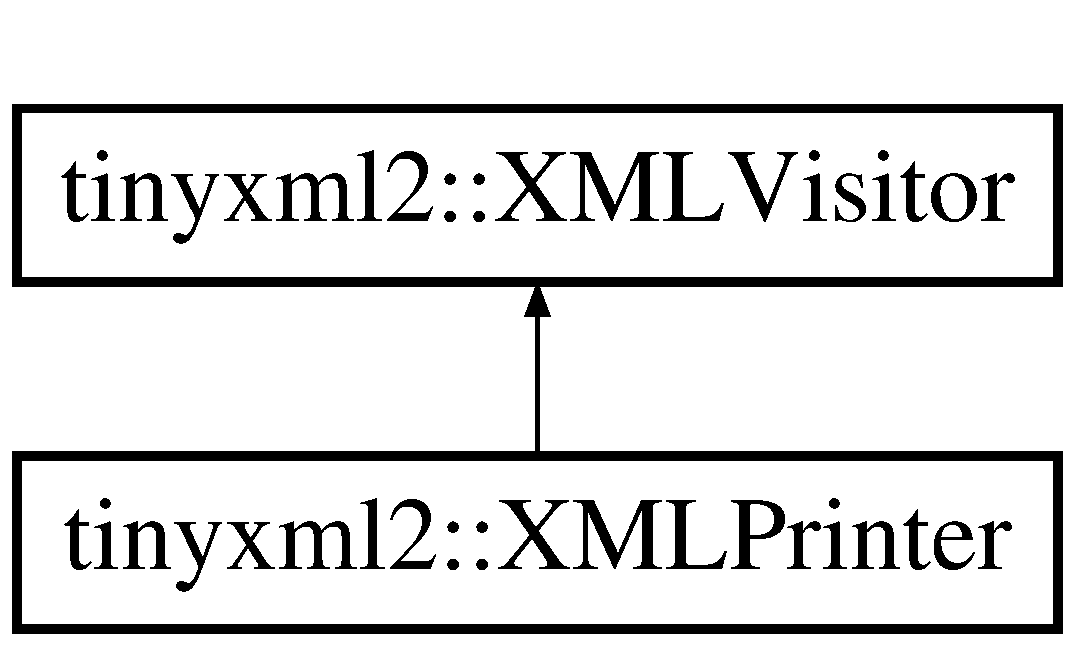
\includegraphics[height=2.000000cm]{classtinyxml2_1_1_x_m_l_printer}
\end{center}
\end{figure}
\subsection*{Public Member Functions}
\begin{DoxyCompactItemize}
\item 
\textbf{ X\+M\+L\+Printer} (F\+I\+LE $\ast$file=0, bool compact=false, int depth=0)
\item 
virtual \textbf{ $\sim$\+X\+M\+L\+Printer} ()
\item 
void \textbf{ Push\+Header} (bool write\+B\+OM, bool write\+Declaration)
\item 
void \textbf{ Open\+Element} (const char $\ast$name, bool compact\+Mode=false)
\item 
void \textbf{ Push\+Attribute} (const char $\ast$name, const char $\ast$value)
\begin{DoxyCompactList}\small\item\em If streaming, add an attribute to an open element. \end{DoxyCompactList}\item 
void \textbf{ Push\+Attribute} (const char $\ast$name, int value)
\item 
void \textbf{ Push\+Attribute} (const char $\ast$name, unsigned value)
\item 
void \textbf{ Push\+Attribute} (const char $\ast$name, int64\+\_\+t value)
\item 
void \textbf{ Push\+Attribute} (const char $\ast$name, bool value)
\item 
void \textbf{ Push\+Attribute} (const char $\ast$name, double value)
\item 
virtual void \textbf{ Close\+Element} (bool compact\+Mode=false)
\begin{DoxyCompactList}\small\item\em If streaming, close the Element. \end{DoxyCompactList}\item 
void \textbf{ Push\+Text} (const char $\ast$text, bool cdata=false)
\begin{DoxyCompactList}\small\item\em Add a text node. \end{DoxyCompactList}\item 
void \textbf{ Push\+Text} (int value)
\begin{DoxyCompactList}\small\item\em Add a text node from an integer. \end{DoxyCompactList}\item 
void \textbf{ Push\+Text} (unsigned value)
\begin{DoxyCompactList}\small\item\em Add a text node from an unsigned. \end{DoxyCompactList}\item 
void \textbf{ Push\+Text} (int64\+\_\+t value)
\begin{DoxyCompactList}\small\item\em Add a text node from an unsigned. \end{DoxyCompactList}\item 
void \textbf{ Push\+Text} (bool value)
\begin{DoxyCompactList}\small\item\em Add a text node from a bool. \end{DoxyCompactList}\item 
void \textbf{ Push\+Text} (float value)
\begin{DoxyCompactList}\small\item\em Add a text node from a float. \end{DoxyCompactList}\item 
void \textbf{ Push\+Text} (double value)
\begin{DoxyCompactList}\small\item\em Add a text node from a double. \end{DoxyCompactList}\item 
void \textbf{ Push\+Comment} (const char $\ast$comment)
\begin{DoxyCompactList}\small\item\em Add a comment. \end{DoxyCompactList}\item 
void \textbf{ Push\+Declaration} (const char $\ast$value)
\item 
void \textbf{ Push\+Unknown} (const char $\ast$value)
\item 
virtual bool \textbf{ Visit\+Enter} (const \textbf{ X\+M\+L\+Document} \&)
\begin{DoxyCompactList}\small\item\em Visit a document. \end{DoxyCompactList}\item 
virtual bool \textbf{ Visit\+Exit} (const \textbf{ X\+M\+L\+Document} \&)
\begin{DoxyCompactList}\small\item\em Visit a document. \end{DoxyCompactList}\item 
virtual bool \textbf{ Visit\+Enter} (const \textbf{ X\+M\+L\+Element} \&element, const \textbf{ X\+M\+L\+Attribute} $\ast$attribute)
\begin{DoxyCompactList}\small\item\em Visit an element. \end{DoxyCompactList}\item 
virtual bool \textbf{ Visit\+Exit} (const \textbf{ X\+M\+L\+Element} \&element)
\begin{DoxyCompactList}\small\item\em Visit an element. \end{DoxyCompactList}\item 
virtual bool \textbf{ Visit} (const \textbf{ X\+M\+L\+Text} \&text)
\begin{DoxyCompactList}\small\item\em Visit a text node. \end{DoxyCompactList}\item 
virtual bool \textbf{ Visit} (const \textbf{ X\+M\+L\+Comment} \&comment)
\begin{DoxyCompactList}\small\item\em Visit a comment node. \end{DoxyCompactList}\item 
virtual bool \textbf{ Visit} (const \textbf{ X\+M\+L\+Declaration} \&declaration)
\begin{DoxyCompactList}\small\item\em Visit a declaration. \end{DoxyCompactList}\item 
virtual bool \textbf{ Visit} (const \textbf{ X\+M\+L\+Unknown} \&unknown)
\begin{DoxyCompactList}\small\item\em Visit an unknown node. \end{DoxyCompactList}\item 
const char $\ast$ \textbf{ C\+Str} () const
\item 
int \textbf{ C\+Str\+Size} () const
\item 
void \textbf{ Clear\+Buffer} ()
\end{DoxyCompactItemize}
\subsection*{Protected Member Functions}
\begin{DoxyCompactItemize}
\item 
virtual bool \textbf{ Compact\+Mode} (const \textbf{ X\+M\+L\+Element} \&)
\item 
virtual void \textbf{ Print\+Space} (int depth)
\item 
void \textbf{ Print} (const char $\ast$format,...)
\item 
void \textbf{ Write} (const char $\ast$data, size\+\_\+t size)
\item 
void \textbf{ Write} (const char $\ast$data)
\item 
void \textbf{ Putc} (char ch)
\item 
void \textbf{ Seal\+Element\+If\+Just\+Opened} ()
\end{DoxyCompactItemize}
\subsection*{Protected Attributes}
\begin{DoxyCompactItemize}
\item 
bool \textbf{ \+\_\+element\+Just\+Opened}
\item 
\textbf{ Dyn\+Array}$<$ const char $\ast$, 10 $>$ \textbf{ \+\_\+stack}
\end{DoxyCompactItemize}
\subsection*{Private Types}
\begin{DoxyCompactItemize}
\item 
enum \{ \textbf{ E\+N\+T\+I\+T\+Y\+\_\+\+R\+A\+N\+GE} = 64, 
\textbf{ B\+U\+F\+\_\+\+S\+I\+ZE} = 200
 \}
\end{DoxyCompactItemize}
\subsection*{Private Member Functions}
\begin{DoxyCompactItemize}
\item 
void \textbf{ Print\+String} (const char $\ast$, bool restricted\+Entity\+Set)
\item 
\textbf{ X\+M\+L\+Printer} (const \textbf{ X\+M\+L\+Printer} \&)
\item 
\textbf{ X\+M\+L\+Printer} \& \textbf{ operator=} (const \textbf{ X\+M\+L\+Printer} \&)
\end{DoxyCompactItemize}
\subsection*{Private Attributes}
\begin{DoxyCompactItemize}
\item 
bool \textbf{ \+\_\+first\+Element}
\item 
F\+I\+LE $\ast$ \textbf{ \+\_\+fp}
\item 
int \textbf{ \+\_\+depth}
\item 
int \textbf{ \+\_\+text\+Depth}
\item 
bool \textbf{ \+\_\+process\+Entities}
\item 
bool \textbf{ \+\_\+compact\+Mode}
\item 
bool \textbf{ \+\_\+entity\+Flag} [\textbf{ E\+N\+T\+I\+T\+Y\+\_\+\+R\+A\+N\+GE}]
\item 
bool \textbf{ \+\_\+restricted\+Entity\+Flag} [\textbf{ E\+N\+T\+I\+T\+Y\+\_\+\+R\+A\+N\+GE}]
\item 
\textbf{ Dyn\+Array}$<$ char, 20 $>$ \textbf{ \+\_\+buffer}
\end{DoxyCompactItemize}


\subsection{Detailed Description}
Printing functionality. The \doxyref{X\+M\+L\+Printer}{p.}{classtinyxml2_1_1_x_m_l_printer} gives you more options than the \doxyref{X\+M\+L\+Document\+::\+Print()}{p.}{classtinyxml2_1_1_x_m_l_document_a867cf5fa3e3ff6ae4847a8b7ee8ec083} method.

It can\+:
\begin{DoxyEnumerate}
\item Print to memory.
\item Print to a file you provide.
\item Print X\+ML without a \doxyref{X\+M\+L\+Document}{p.}{classtinyxml2_1_1_x_m_l_document}.
\end{DoxyEnumerate}

Print to Memory

\begin{DoxyVerb}XMLPrinter printer;
doc.Print( &printer );
SomeFunction( printer.CStr() );
\end{DoxyVerb}


Print to a File

You provide the file pointer. \begin{DoxyVerb}XMLPrinter printer( fp );
doc.Print( &printer );
\end{DoxyVerb}


Print without a \doxyref{X\+M\+L\+Document}{p.}{classtinyxml2_1_1_x_m_l_document}

When loading, an X\+ML parser is very useful. However, sometimes when saving, it just gets in the way. The code is often set up for streaming, and constructing the D\+OM is just overhead.

The Printer supports the streaming case. The following code prints out a trivially simple X\+ML file without ever creating an X\+ML document.

\begin{DoxyVerb}XMLPrinter printer( fp );
printer.OpenElement( "foo" );
printer.PushAttribute( "foo", "bar" );
printer.CloseElement();
\end{DoxyVerb}
 

Definition at line 2175 of file tinyxml2.\+h.



\subsection{Member Enumeration Documentation}
\mbox{\label{classtinyxml2_1_1_x_m_l_printer_ac9049bee10d230eb31ff7d146d538f7a}} 
\subsubsection{anonymous enum}
{\footnotesize\ttfamily anonymous enum\hspace{0.3cm}{\ttfamily [private]}}

\begin{DoxyEnumFields}{Enumerator}
\raisebox{\heightof{T}}[0pt][0pt]{\index{ENTITY\_RANGE@{ENTITY\_RANGE}!tinyxml2::XMLPrinter@{tinyxml2::XMLPrinter}}\index{tinyxml2::XMLPrinter@{tinyxml2::XMLPrinter}!ENTITY\_RANGE@{ENTITY\_RANGE}}}\mbox{\label{classtinyxml2_1_1_x_m_l_printer_ac9049bee10d230eb31ff7d146d538f7aa2ddc02813235fe451809606959166db5}} 
E\+N\+T\+I\+T\+Y\+\_\+\+R\+A\+N\+GE&\\
\hline

\raisebox{\heightof{T}}[0pt][0pt]{\index{BUF\_SIZE@{BUF\_SIZE}!tinyxml2::XMLPrinter@{tinyxml2::XMLPrinter}}\index{tinyxml2::XMLPrinter@{tinyxml2::XMLPrinter}!BUF\_SIZE@{BUF\_SIZE}}}\mbox{\label{classtinyxml2_1_1_x_m_l_printer_ac9049bee10d230eb31ff7d146d538f7aa1f747a8fb39ceb2e711c3798058fb632}} 
B\+U\+F\+\_\+\+S\+I\+ZE&\\
\hline

\end{DoxyEnumFields}


Definition at line 2288 of file tinyxml2.\+h.



\subsection{Constructor \& Destructor Documentation}
\mbox{\label{classtinyxml2_1_1_x_m_l_printer_aa6d3841c069085f5b8a27bc7103c04f7}} 
\index{tinyxml2::XMLPrinter@{tinyxml2::XMLPrinter}!XMLPrinter@{XMLPrinter}}
\index{XMLPrinter@{XMLPrinter}!tinyxml2::XMLPrinter@{tinyxml2::XMLPrinter}}
\subsubsection{XMLPrinter()\hspace{0.1cm}{\footnotesize\ttfamily [1/2]}}
{\footnotesize\ttfamily tinyxml2\+::\+X\+M\+L\+Printer\+::\+X\+M\+L\+Printer (\begin{DoxyParamCaption}\item[{F\+I\+LE $\ast$}]{file = {\ttfamily 0},  }\item[{bool}]{compact = {\ttfamily false},  }\item[{int}]{depth = {\ttfamily 0} }\end{DoxyParamCaption})}

Construct the printer. If the F\+I\+L\+E$\ast$ is specified, this will print to the F\+I\+LE. Else it will print to memory, and the result is available in \doxyref{C\+Str()}{p.}{classtinyxml2_1_1_x_m_l_printer_a180671d73844f159f2d4aafbc11d106e}. If \textquotesingle{}compact\textquotesingle{} is set to true, then output is created with only required whitespace and newlines. 

Definition at line 2410 of file tinyxml2.\+cpp.



References \+\_\+buffer, \+\_\+entity\+Flag, \+\_\+restricted\+Entity\+Flag, tinyxml2\+::entities, E\+N\+T\+I\+T\+Y\+\_\+\+R\+A\+N\+GE, tinyxml2\+::\+N\+U\+M\+\_\+\+E\+N\+T\+I\+T\+I\+ES, tinyxml2\+::\+Dyn\+Array$<$ T, I\+N\+I\+T\+I\+A\+L\+\_\+\+S\+I\+Z\+E $>$\+::\+Push(), T\+I\+X\+M\+L\+A\+S\+S\+E\+RT, and tinyxml2\+::\+Entity\+::value.

\mbox{\label{classtinyxml2_1_1_x_m_l_printer_af4caefa48ea6436898fb1807de8d14c0}} 
\index{tinyxml2::XMLPrinter@{tinyxml2::XMLPrinter}!````~XMLPrinter@{$\sim$XMLPrinter}}
\index{````~XMLPrinter@{$\sim$XMLPrinter}!tinyxml2::XMLPrinter@{tinyxml2::XMLPrinter}}
\subsubsection{$\sim$XMLPrinter()}
{\footnotesize\ttfamily virtual tinyxml2\+::\+X\+M\+L\+Printer\+::$\sim$\+X\+M\+L\+Printer (\begin{DoxyParamCaption}{ }\end{DoxyParamCaption})\hspace{0.3cm}{\ttfamily [inline]}, {\ttfamily [virtual]}}



Definition at line 2185 of file tinyxml2.\+h.

\mbox{\label{classtinyxml2_1_1_x_m_l_printer_a157706836c056febc4022dc540a47982}} 
\index{tinyxml2::XMLPrinter@{tinyxml2::XMLPrinter}!XMLPrinter@{XMLPrinter}}
\index{XMLPrinter@{XMLPrinter}!tinyxml2::XMLPrinter@{tinyxml2::XMLPrinter}}
\subsubsection{XMLPrinter()\hspace{0.1cm}{\footnotesize\ttfamily [2/2]}}
{\footnotesize\ttfamily tinyxml2\+::\+X\+M\+L\+Printer\+::\+X\+M\+L\+Printer (\begin{DoxyParamCaption}\item[{const \textbf{ X\+M\+L\+Printer} \&}]{ }\end{DoxyParamCaption})\hspace{0.3cm}{\ttfamily [private]}}



\subsection{Member Function Documentation}
\mbox{\label{classtinyxml2_1_1_x_m_l_printer_a216157765b7267bf389975b1cbf9a909}} 
\index{tinyxml2::XMLPrinter@{tinyxml2::XMLPrinter}!ClearBuffer@{ClearBuffer}}
\index{ClearBuffer@{ClearBuffer}!tinyxml2::XMLPrinter@{tinyxml2::XMLPrinter}}
\subsubsection{ClearBuffer()}
{\footnotesize\ttfamily void tinyxml2\+::\+X\+M\+L\+Printer\+::\+Clear\+Buffer (\begin{DoxyParamCaption}{ }\end{DoxyParamCaption})\hspace{0.3cm}{\ttfamily [inline]}}

If in print to memory mode, reset the buffer to the beginning. 

Definition at line 2256 of file tinyxml2.\+h.

\mbox{\label{classtinyxml2_1_1_x_m_l_printer_af1fb439e5d800999646f333fa2f0699a}} 
\index{tinyxml2::XMLPrinter@{tinyxml2::XMLPrinter}!CloseElement@{CloseElement}}
\index{CloseElement@{CloseElement}!tinyxml2::XMLPrinter@{tinyxml2::XMLPrinter}}
\subsubsection{CloseElement()}
{\footnotesize\ttfamily void tinyxml2\+::\+X\+M\+L\+Printer\+::\+Close\+Element (\begin{DoxyParamCaption}\item[{bool}]{compact\+Mode = {\ttfamily false} }\end{DoxyParamCaption})\hspace{0.3cm}{\ttfamily [virtual]}}



If streaming, close the Element. 



Definition at line 2633 of file tinyxml2.\+cpp.



References \+\_\+depth, \+\_\+element\+Just\+Opened, \+\_\+stack, \+\_\+text\+Depth, tinyxml2\+::\+Dyn\+Array$<$ T, I\+N\+I\+T\+I\+A\+L\+\_\+\+S\+I\+Z\+E $>$\+::\+Pop(), Print\+Space(), Putc(), and Write().



Referenced by Visit\+Exit().

\mbox{\label{classtinyxml2_1_1_x_m_l_printer_a38e1ed5a779bdf63eda9e808f7a6de66}} 
\index{tinyxml2::XMLPrinter@{tinyxml2::XMLPrinter}!CompactMode@{CompactMode}}
\index{CompactMode@{CompactMode}!tinyxml2::XMLPrinter@{tinyxml2::XMLPrinter}}
\subsubsection{CompactMode()}
{\footnotesize\ttfamily virtual bool tinyxml2\+::\+X\+M\+L\+Printer\+::\+Compact\+Mode (\begin{DoxyParamCaption}\item[{const \textbf{ X\+M\+L\+Element} \&}]{ }\end{DoxyParamCaption})\hspace{0.3cm}{\ttfamily [inline]}, {\ttfamily [protected]}, {\ttfamily [virtual]}}



Definition at line 2263 of file tinyxml2.\+h.



Referenced by Visit\+Enter(), and Visit\+Exit().

\mbox{\label{classtinyxml2_1_1_x_m_l_printer_a180671d73844f159f2d4aafbc11d106e}} 
\index{tinyxml2::XMLPrinter@{tinyxml2::XMLPrinter}!CStr@{CStr}}
\index{CStr@{CStr}!tinyxml2::XMLPrinter@{tinyxml2::XMLPrinter}}
\subsubsection{CStr()}
{\footnotesize\ttfamily const char$\ast$ tinyxml2\+::\+X\+M\+L\+Printer\+::\+C\+Str (\begin{DoxyParamCaption}{ }\end{DoxyParamCaption}) const\hspace{0.3cm}{\ttfamily [inline]}}

If in print to memory mode, return a pointer to the X\+ML file in memory. 

Definition at line 2241 of file tinyxml2.\+h.

\mbox{\label{classtinyxml2_1_1_x_m_l_printer_a3256cf3523d4898b91abb18b924be04c}} 
\index{tinyxml2::XMLPrinter@{tinyxml2::XMLPrinter}!CStrSize@{CStrSize}}
\index{CStrSize@{CStrSize}!tinyxml2::XMLPrinter@{tinyxml2::XMLPrinter}}
\subsubsection{CStrSize()}
{\footnotesize\ttfamily int tinyxml2\+::\+X\+M\+L\+Printer\+::\+C\+Str\+Size (\begin{DoxyParamCaption}{ }\end{DoxyParamCaption}) const\hspace{0.3cm}{\ttfamily [inline]}}

If in print to memory mode, return the size of the X\+ML file in memory. (Note the size returned includes the terminating null.) 

Definition at line 2249 of file tinyxml2.\+h.

\mbox{\label{classtinyxml2_1_1_x_m_l_printer_a20fb06c83bd13e5140d7dd13af06c010}} 
\index{tinyxml2::XMLPrinter@{tinyxml2::XMLPrinter}!OpenElement@{OpenElement}}
\index{OpenElement@{OpenElement}!tinyxml2::XMLPrinter@{tinyxml2::XMLPrinter}}
\subsubsection{OpenElement()}
{\footnotesize\ttfamily void tinyxml2\+::\+X\+M\+L\+Printer\+::\+Open\+Element (\begin{DoxyParamCaption}\item[{const char $\ast$}]{name,  }\item[{bool}]{compact\+Mode = {\ttfamily false} }\end{DoxyParamCaption})}

If streaming, start writing an element. The element must be closed with \doxyref{Close\+Element()}{p.}{classtinyxml2_1_1_x_m_l_printer_af1fb439e5d800999646f333fa2f0699a} 

Definition at line 2561 of file tinyxml2.\+cpp.



References \+\_\+depth, \+\_\+element\+Just\+Opened, \+\_\+first\+Element, \+\_\+stack, \+\_\+text\+Depth, Print\+Space(), tinyxml2\+::\+Dyn\+Array$<$ T, I\+N\+I\+T\+I\+A\+L\+\_\+\+S\+I\+Z\+E $>$\+::\+Push(), Putc(), Seal\+Element\+If\+Just\+Opened(), and Write().



Referenced by Visit\+Enter().

\mbox{\label{classtinyxml2_1_1_x_m_l_printer_a7706d90e6cd31ef081742e8344b3f9bc}} 
\index{tinyxml2::XMLPrinter@{tinyxml2::XMLPrinter}!operator=@{operator=}}
\index{operator=@{operator=}!tinyxml2::XMLPrinter@{tinyxml2::XMLPrinter}}
\subsubsection{operator=()}
{\footnotesize\ttfamily \textbf{ X\+M\+L\+Printer}\& tinyxml2\+::\+X\+M\+L\+Printer\+::operator= (\begin{DoxyParamCaption}\item[{const \textbf{ X\+M\+L\+Printer} \&}]{ }\end{DoxyParamCaption})\hspace{0.3cm}{\ttfamily [private]}}

\mbox{\label{classtinyxml2_1_1_x_m_l_printer_ab30210a7f32e45634e7a45137bf6fdf6}} 
\index{tinyxml2::XMLPrinter@{tinyxml2::XMLPrinter}!Print@{Print}}
\index{Print@{Print}!tinyxml2::XMLPrinter@{tinyxml2::XMLPrinter}}
\subsubsection{Print()}
{\footnotesize\ttfamily void tinyxml2\+::\+X\+M\+L\+Printer\+::\+Print (\begin{DoxyParamCaption}\item[{const char $\ast$}]{format,  }\item[{}]{... }\end{DoxyParamCaption})\hspace{0.3cm}{\ttfamily [protected]}}



Definition at line 2438 of file tinyxml2.\+cpp.



References \+\_\+buffer, \+\_\+fp, tinyxml2\+::\+Dyn\+Array$<$ T, I\+N\+I\+T\+I\+A\+L\+\_\+\+S\+I\+Z\+E $>$\+::\+Push\+Arr(), tinyxml2\+::\+Dyn\+Array$<$ T, I\+N\+I\+T\+I\+A\+L\+\_\+\+S\+I\+Z\+E $>$\+::\+Size(), T\+I\+X\+M\+L\+\_\+\+V\+S\+C\+P\+R\+I\+N\+T\+F(), T\+I\+X\+M\+L\+\_\+\+V\+S\+N\+P\+R\+I\+N\+TF, and T\+I\+X\+M\+L\+A\+S\+S\+E\+RT.

\mbox{\label{classtinyxml2_1_1_x_m_l_printer_a1c4b2ccbe4fdb316d54f5a93f3559260}} 
\index{tinyxml2::XMLPrinter@{tinyxml2::XMLPrinter}!PrintSpace@{PrintSpace}}
\index{PrintSpace@{PrintSpace}!tinyxml2::XMLPrinter@{tinyxml2::XMLPrinter}}
\subsubsection{PrintSpace()}
{\footnotesize\ttfamily void tinyxml2\+::\+X\+M\+L\+Printer\+::\+Print\+Space (\begin{DoxyParamCaption}\item[{int}]{depth }\end{DoxyParamCaption})\hspace{0.3cm}{\ttfamily [protected]}, {\ttfamily [virtual]}}

Prints out the space before an element. You may override to change the space and tabs used. A \doxyref{Print\+Space()}{p.}{classtinyxml2_1_1_x_m_l_printer_a1c4b2ccbe4fdb316d54f5a93f3559260} override should call \doxyref{Print()}{p.}{classtinyxml2_1_1_x_m_l_printer_ab30210a7f32e45634e7a45137bf6fdf6}. 

Definition at line 2486 of file tinyxml2.\+cpp.



References Write().



Referenced by Close\+Element(), Open\+Element(), Push\+Comment(), Push\+Declaration(), and Push\+Unknown().

\mbox{\label{classtinyxml2_1_1_x_m_l_printer_a5495e504053f63f2c4d603327314fa91}} 
\index{tinyxml2::XMLPrinter@{tinyxml2::XMLPrinter}!PrintString@{PrintString}}
\index{PrintString@{PrintString}!tinyxml2::XMLPrinter@{tinyxml2::XMLPrinter}}
\subsubsection{PrintString()}
{\footnotesize\ttfamily void tinyxml2\+::\+X\+M\+L\+Printer\+::\+Print\+String (\begin{DoxyParamCaption}\item[{const char $\ast$}]{p,  }\item[{bool}]{restricted\+Entity\+Set }\end{DoxyParamCaption})\hspace{0.3cm}{\ttfamily [private]}}



Definition at line 2494 of file tinyxml2.\+cpp.



References \+\_\+entity\+Flag, \+\_\+process\+Entities, \+\_\+restricted\+Entity\+Flag, tinyxml2\+::entities, E\+N\+T\+I\+T\+Y\+\_\+\+R\+A\+N\+GE, tinyxml2\+::\+N\+U\+M\+\_\+\+E\+N\+T\+I\+T\+I\+ES, Putc(), T\+I\+X\+M\+L\+A\+S\+S\+E\+RT, and Write().



Referenced by Push\+Attribute(), and Push\+Text().

\mbox{\label{classtinyxml2_1_1_x_m_l_printer_a9a4e2c9348b42e147629d5a99f4af3f0}} 
\index{tinyxml2::XMLPrinter@{tinyxml2::XMLPrinter}!PushAttribute@{PushAttribute}}
\index{PushAttribute@{PushAttribute}!tinyxml2::XMLPrinter@{tinyxml2::XMLPrinter}}
\subsubsection{PushAttribute()\hspace{0.1cm}{\footnotesize\ttfamily [1/6]}}
{\footnotesize\ttfamily void tinyxml2\+::\+X\+M\+L\+Printer\+::\+Push\+Attribute (\begin{DoxyParamCaption}\item[{const char $\ast$}]{name,  }\item[{const char $\ast$}]{value }\end{DoxyParamCaption})}



If streaming, add an attribute to an open element. 



Definition at line 2582 of file tinyxml2.\+cpp.



References \+\_\+element\+Just\+Opened, Print\+String(), Putc(), T\+I\+X\+M\+L\+A\+S\+S\+E\+RT, and Write().



Referenced by Push\+Attribute(), and Visit\+Enter().

\mbox{\label{classtinyxml2_1_1_x_m_l_printer_a69120c82088597372d28d0a98f2ee7a1}} 
\index{tinyxml2::XMLPrinter@{tinyxml2::XMLPrinter}!PushAttribute@{PushAttribute}}
\index{PushAttribute@{PushAttribute}!tinyxml2::XMLPrinter@{tinyxml2::XMLPrinter}}
\subsubsection{PushAttribute()\hspace{0.1cm}{\footnotesize\ttfamily [2/6]}}
{\footnotesize\ttfamily void tinyxml2\+::\+X\+M\+L\+Printer\+::\+Push\+Attribute (\begin{DoxyParamCaption}\item[{const char $\ast$}]{name,  }\item[{int}]{value }\end{DoxyParamCaption})}



Definition at line 2593 of file tinyxml2.\+cpp.



References B\+U\+F\+\_\+\+S\+I\+ZE, Push\+Attribute(), and tinyxml2\+::\+X\+M\+L\+Util\+::\+To\+Str().

\mbox{\label{classtinyxml2_1_1_x_m_l_printer_aa41039e51990aaf5342f3e0575a692c4}} 
\index{tinyxml2::XMLPrinter@{tinyxml2::XMLPrinter}!PushAttribute@{PushAttribute}}
\index{PushAttribute@{PushAttribute}!tinyxml2::XMLPrinter@{tinyxml2::XMLPrinter}}
\subsubsection{PushAttribute()\hspace{0.1cm}{\footnotesize\ttfamily [3/6]}}
{\footnotesize\ttfamily void tinyxml2\+::\+X\+M\+L\+Printer\+::\+Push\+Attribute (\begin{DoxyParamCaption}\item[{const char $\ast$}]{name,  }\item[{unsigned}]{value }\end{DoxyParamCaption})}



Definition at line 2601 of file tinyxml2.\+cpp.



References B\+U\+F\+\_\+\+S\+I\+ZE, Push\+Attribute(), and tinyxml2\+::\+X\+M\+L\+Util\+::\+To\+Str().

\mbox{\label{classtinyxml2_1_1_x_m_l_printer_a9bc2fe21a83a70e6aa0415f2034ecbff}} 
\index{tinyxml2::XMLPrinter@{tinyxml2::XMLPrinter}!PushAttribute@{PushAttribute}}
\index{PushAttribute@{PushAttribute}!tinyxml2::XMLPrinter@{tinyxml2::XMLPrinter}}
\subsubsection{PushAttribute()\hspace{0.1cm}{\footnotesize\ttfamily [4/6]}}
{\footnotesize\ttfamily void tinyxml2\+::\+X\+M\+L\+Printer\+::\+Push\+Attribute (\begin{DoxyParamCaption}\item[{const char $\ast$}]{name,  }\item[{int64\+\_\+t}]{value }\end{DoxyParamCaption})}



Definition at line 2609 of file tinyxml2.\+cpp.



References B\+U\+F\+\_\+\+S\+I\+ZE, Push\+Attribute(), and tinyxml2\+::\+X\+M\+L\+Util\+::\+To\+Str().

\mbox{\label{classtinyxml2_1_1_x_m_l_printer_a51f7950d7b7a19f0d3a0d549a318d45f}} 
\index{tinyxml2::XMLPrinter@{tinyxml2::XMLPrinter}!PushAttribute@{PushAttribute}}
\index{PushAttribute@{PushAttribute}!tinyxml2::XMLPrinter@{tinyxml2::XMLPrinter}}
\subsubsection{PushAttribute()\hspace{0.1cm}{\footnotesize\ttfamily [5/6]}}
{\footnotesize\ttfamily void tinyxml2\+::\+X\+M\+L\+Printer\+::\+Push\+Attribute (\begin{DoxyParamCaption}\item[{const char $\ast$}]{name,  }\item[{bool}]{value }\end{DoxyParamCaption})}



Definition at line 2617 of file tinyxml2.\+cpp.



References B\+U\+F\+\_\+\+S\+I\+ZE, Push\+Attribute(), and tinyxml2\+::\+X\+M\+L\+Util\+::\+To\+Str().

\mbox{\label{classtinyxml2_1_1_x_m_l_printer_a1714867af40e68ca404c3e84b6cac2a6}} 
\index{tinyxml2::XMLPrinter@{tinyxml2::XMLPrinter}!PushAttribute@{PushAttribute}}
\index{PushAttribute@{PushAttribute}!tinyxml2::XMLPrinter@{tinyxml2::XMLPrinter}}
\subsubsection{PushAttribute()\hspace{0.1cm}{\footnotesize\ttfamily [6/6]}}
{\footnotesize\ttfamily void tinyxml2\+::\+X\+M\+L\+Printer\+::\+Push\+Attribute (\begin{DoxyParamCaption}\item[{const char $\ast$}]{name,  }\item[{double}]{value }\end{DoxyParamCaption})}



Definition at line 2625 of file tinyxml2.\+cpp.



References B\+U\+F\+\_\+\+S\+I\+ZE, Push\+Attribute(), and tinyxml2\+::\+X\+M\+L\+Util\+::\+To\+Str().

\mbox{\label{classtinyxml2_1_1_x_m_l_printer_afc8416814219591c2fd5656e0c233140}} 
\index{tinyxml2::XMLPrinter@{tinyxml2::XMLPrinter}!PushComment@{PushComment}}
\index{PushComment@{PushComment}!tinyxml2::XMLPrinter@{tinyxml2::XMLPrinter}}
\subsubsection{PushComment()}
{\footnotesize\ttfamily void tinyxml2\+::\+X\+M\+L\+Printer\+::\+Push\+Comment (\begin{DoxyParamCaption}\item[{const char $\ast$}]{comment }\end{DoxyParamCaption})}



Add a comment. 



Definition at line 2733 of file tinyxml2.\+cpp.



References \+\_\+compact\+Mode, \+\_\+depth, \+\_\+first\+Element, \+\_\+text\+Depth, Print\+Space(), Putc(), Seal\+Element\+If\+Just\+Opened(), and Write().



Referenced by Visit().

\mbox{\label{classtinyxml2_1_1_x_m_l_printer_a2fe3565e262594efc6c0276723c83fe7}} 
\index{tinyxml2::XMLPrinter@{tinyxml2::XMLPrinter}!PushDeclaration@{PushDeclaration}}
\index{PushDeclaration@{PushDeclaration}!tinyxml2::XMLPrinter@{tinyxml2::XMLPrinter}}
\subsubsection{PushDeclaration()}
{\footnotesize\ttfamily void tinyxml2\+::\+X\+M\+L\+Printer\+::\+Push\+Declaration (\begin{DoxyParamCaption}\item[{const char $\ast$}]{value }\end{DoxyParamCaption})}



Definition at line 2748 of file tinyxml2.\+cpp.



References \+\_\+compact\+Mode, \+\_\+depth, \+\_\+first\+Element, \+\_\+text\+Depth, Print\+Space(), Putc(), Seal\+Element\+If\+Just\+Opened(), and Write().



Referenced by Push\+Header(), and Visit().

\mbox{\label{classtinyxml2_1_1_x_m_l_printer_a178c608ce8476043d5d6513819cde903}} 
\index{tinyxml2::XMLPrinter@{tinyxml2::XMLPrinter}!PushHeader@{PushHeader}}
\index{PushHeader@{PushHeader}!tinyxml2::XMLPrinter@{tinyxml2::XMLPrinter}}
\subsubsection{PushHeader()}
{\footnotesize\ttfamily void tinyxml2\+::\+X\+M\+L\+Printer\+::\+Push\+Header (\begin{DoxyParamCaption}\item[{bool}]{write\+B\+OM,  }\item[{bool}]{write\+Declaration }\end{DoxyParamCaption})}

If streaming, write the B\+OM and declaration. 

Definition at line 2549 of file tinyxml2.\+cpp.



References Push\+Declaration(), T\+I\+X\+M\+L\+\_\+\+U\+T\+F\+\_\+\+L\+E\+A\+D\+\_\+0, T\+I\+X\+M\+L\+\_\+\+U\+T\+F\+\_\+\+L\+E\+A\+D\+\_\+1, T\+I\+X\+M\+L\+\_\+\+U\+T\+F\+\_\+\+L\+E\+A\+D\+\_\+2, and Write().



Referenced by Visit\+Enter().

\mbox{\label{classtinyxml2_1_1_x_m_l_printer_a1cc16a9362df4332012cb13cff6441b3}} 
\index{tinyxml2::XMLPrinter@{tinyxml2::XMLPrinter}!PushText@{PushText}}
\index{PushText@{PushText}!tinyxml2::XMLPrinter@{tinyxml2::XMLPrinter}}
\subsubsection{PushText()\hspace{0.1cm}{\footnotesize\ttfamily [1/7]}}
{\footnotesize\ttfamily void tinyxml2\+::\+X\+M\+L\+Printer\+::\+Push\+Text (\begin{DoxyParamCaption}\item[{const char $\ast$}]{text,  }\item[{bool}]{cdata = {\ttfamily false} }\end{DoxyParamCaption})}



Add a text node. 



Definition at line 2671 of file tinyxml2.\+cpp.



References \+\_\+depth, \+\_\+text\+Depth, Print\+String(), Seal\+Element\+If\+Just\+Opened(), and Write().



Referenced by Push\+Text(), and Visit().

\mbox{\label{classtinyxml2_1_1_x_m_l_printer_a3e0d4d78de25d4cf081009e1431cea7e}} 
\index{tinyxml2::XMLPrinter@{tinyxml2::XMLPrinter}!PushText@{PushText}}
\index{PushText@{PushText}!tinyxml2::XMLPrinter@{tinyxml2::XMLPrinter}}
\subsubsection{PushText()\hspace{0.1cm}{\footnotesize\ttfamily [2/7]}}
{\footnotesize\ttfamily void tinyxml2\+::\+X\+M\+L\+Printer\+::\+Push\+Text (\begin{DoxyParamCaption}\item[{int}]{value }\end{DoxyParamCaption})}



Add a text node from an integer. 



Definition at line 2693 of file tinyxml2.\+cpp.



References B\+U\+F\+\_\+\+S\+I\+ZE, Push\+Text(), and tinyxml2\+::\+X\+M\+L\+Util\+::\+To\+Str().

\mbox{\label{classtinyxml2_1_1_x_m_l_printer_a661fb50e7e0a4918d2d259cb0fae647e}} 
\index{tinyxml2::XMLPrinter@{tinyxml2::XMLPrinter}!PushText@{PushText}}
\index{PushText@{PushText}!tinyxml2::XMLPrinter@{tinyxml2::XMLPrinter}}
\subsubsection{PushText()\hspace{0.1cm}{\footnotesize\ttfamily [3/7]}}
{\footnotesize\ttfamily void tinyxml2\+::\+X\+M\+L\+Printer\+::\+Push\+Text (\begin{DoxyParamCaption}\item[{unsigned}]{value }\end{DoxyParamCaption})}



Add a text node from an unsigned. 



Definition at line 2701 of file tinyxml2.\+cpp.



References B\+U\+F\+\_\+\+S\+I\+ZE, Push\+Text(), and tinyxml2\+::\+X\+M\+L\+Util\+::\+To\+Str().

\mbox{\label{classtinyxml2_1_1_x_m_l_printer_a96b0a0bfe105154a0a6c37d725258f0a}} 
\index{tinyxml2::XMLPrinter@{tinyxml2::XMLPrinter}!PushText@{PushText}}
\index{PushText@{PushText}!tinyxml2::XMLPrinter@{tinyxml2::XMLPrinter}}
\subsubsection{PushText()\hspace{0.1cm}{\footnotesize\ttfamily [4/7]}}
{\footnotesize\ttfamily void tinyxml2\+::\+X\+M\+L\+Printer\+::\+Push\+Text (\begin{DoxyParamCaption}\item[{int64\+\_\+t}]{value }\end{DoxyParamCaption})}



Add a text node from an unsigned. 



Definition at line 2686 of file tinyxml2.\+cpp.



References B\+U\+F\+\_\+\+S\+I\+ZE, Push\+Text(), and tinyxml2\+::\+X\+M\+L\+Util\+::\+To\+Str().

\mbox{\label{classtinyxml2_1_1_x_m_l_printer_a4390e5fa1ed05189a8686647345ab29f}} 
\index{tinyxml2::XMLPrinter@{tinyxml2::XMLPrinter}!PushText@{PushText}}
\index{PushText@{PushText}!tinyxml2::XMLPrinter@{tinyxml2::XMLPrinter}}
\subsubsection{PushText()\hspace{0.1cm}{\footnotesize\ttfamily [5/7]}}
{\footnotesize\ttfamily void tinyxml2\+::\+X\+M\+L\+Printer\+::\+Push\+Text (\begin{DoxyParamCaption}\item[{bool}]{value }\end{DoxyParamCaption})}



Add a text node from a bool. 



Definition at line 2709 of file tinyxml2.\+cpp.



References B\+U\+F\+\_\+\+S\+I\+ZE, Push\+Text(), and tinyxml2\+::\+X\+M\+L\+Util\+::\+To\+Str().

\mbox{\label{classtinyxml2_1_1_x_m_l_printer_a1dbb1390e829d0673af66b9cd1928bd7}} 
\index{tinyxml2::XMLPrinter@{tinyxml2::XMLPrinter}!PushText@{PushText}}
\index{PushText@{PushText}!tinyxml2::XMLPrinter@{tinyxml2::XMLPrinter}}
\subsubsection{PushText()\hspace{0.1cm}{\footnotesize\ttfamily [6/7]}}
{\footnotesize\ttfamily void tinyxml2\+::\+X\+M\+L\+Printer\+::\+Push\+Text (\begin{DoxyParamCaption}\item[{float}]{value }\end{DoxyParamCaption})}



Add a text node from a float. 



Definition at line 2717 of file tinyxml2.\+cpp.



References B\+U\+F\+\_\+\+S\+I\+ZE, Push\+Text(), and tinyxml2\+::\+X\+M\+L\+Util\+::\+To\+Str().

\mbox{\label{classtinyxml2_1_1_x_m_l_printer_aa715302dfc09473c77c853cbd5431965}} 
\index{tinyxml2::XMLPrinter@{tinyxml2::XMLPrinter}!PushText@{PushText}}
\index{PushText@{PushText}!tinyxml2::XMLPrinter@{tinyxml2::XMLPrinter}}
\subsubsection{PushText()\hspace{0.1cm}{\footnotesize\ttfamily [7/7]}}
{\footnotesize\ttfamily void tinyxml2\+::\+X\+M\+L\+Printer\+::\+Push\+Text (\begin{DoxyParamCaption}\item[{double}]{value }\end{DoxyParamCaption})}



Add a text node from a double. 



Definition at line 2725 of file tinyxml2.\+cpp.



References B\+U\+F\+\_\+\+S\+I\+ZE, Push\+Text(), and tinyxml2\+::\+X\+M\+L\+Util\+::\+To\+Str().

\mbox{\label{classtinyxml2_1_1_x_m_l_printer_ab1efc6d1548505e9984185f58f54b713}} 
\index{tinyxml2::XMLPrinter@{tinyxml2::XMLPrinter}!PushUnknown@{PushUnknown}}
\index{PushUnknown@{PushUnknown}!tinyxml2::XMLPrinter@{tinyxml2::XMLPrinter}}
\subsubsection{PushUnknown()}
{\footnotesize\ttfamily void tinyxml2\+::\+X\+M\+L\+Printer\+::\+Push\+Unknown (\begin{DoxyParamCaption}\item[{const char $\ast$}]{value }\end{DoxyParamCaption})}



Definition at line 2763 of file tinyxml2.\+cpp.



References \+\_\+compact\+Mode, \+\_\+depth, \+\_\+first\+Element, \+\_\+text\+Depth, Print\+Space(), Putc(), Seal\+Element\+If\+Just\+Opened(), and Write().



Referenced by Visit().

\mbox{\label{classtinyxml2_1_1_x_m_l_printer_a9567b0218169ba59794f171ae2f9944c}} 
\index{tinyxml2::XMLPrinter@{tinyxml2::XMLPrinter}!Putc@{Putc}}
\index{Putc@{Putc}!tinyxml2::XMLPrinter@{tinyxml2::XMLPrinter}}
\subsubsection{Putc()}
{\footnotesize\ttfamily void tinyxml2\+::\+X\+M\+L\+Printer\+::\+Putc (\begin{DoxyParamCaption}\item[{char}]{ch }\end{DoxyParamCaption})\hspace{0.3cm}{\ttfamily [protected]}}



Definition at line 2473 of file tinyxml2.\+cpp.



References \+\_\+buffer, \+\_\+fp, and tinyxml2\+::\+Dyn\+Array$<$ T, I\+N\+I\+T\+I\+A\+L\+\_\+\+S\+I\+Z\+E $>$\+::\+Push\+Arr().



Referenced by Close\+Element(), Open\+Element(), Print\+String(), Push\+Attribute(), Push\+Comment(), Push\+Declaration(), Push\+Unknown(), and Seal\+Element\+If\+Just\+Opened().

\mbox{\label{classtinyxml2_1_1_x_m_l_printer_ac6e2c72c5d796f5b4de6ce81ca95e3fa}} 
\index{tinyxml2::XMLPrinter@{tinyxml2::XMLPrinter}!SealElementIfJustOpened@{SealElementIfJustOpened}}
\index{SealElementIfJustOpened@{SealElementIfJustOpened}!tinyxml2::XMLPrinter@{tinyxml2::XMLPrinter}}
\subsubsection{SealElementIfJustOpened()}
{\footnotesize\ttfamily void tinyxml2\+::\+X\+M\+L\+Printer\+::\+Seal\+Element\+If\+Just\+Opened (\begin{DoxyParamCaption}{ }\end{DoxyParamCaption})\hspace{0.3cm}{\ttfamily [protected]}}



Definition at line 2661 of file tinyxml2.\+cpp.



References \+\_\+element\+Just\+Opened, and Putc().



Referenced by Open\+Element(), Push\+Comment(), Push\+Declaration(), Push\+Text(), and Push\+Unknown().

\mbox{\label{classtinyxml2_1_1_x_m_l_printer_adc0e42b4f6fcb90a95630c79575d030b}} 
\index{tinyxml2::XMLPrinter@{tinyxml2::XMLPrinter}!Visit@{Visit}}
\index{Visit@{Visit}!tinyxml2::XMLPrinter@{tinyxml2::XMLPrinter}}
\subsubsection{Visit()\hspace{0.1cm}{\footnotesize\ttfamily [1/4]}}
{\footnotesize\ttfamily bool tinyxml2\+::\+X\+M\+L\+Printer\+::\+Visit (\begin{DoxyParamCaption}\item[{const \textbf{ X\+M\+L\+Text} \&}]{ }\end{DoxyParamCaption})\hspace{0.3cm}{\ttfamily [virtual]}}



Visit a text node. 



Reimplemented from \textbf{ tinyxml2\+::\+X\+M\+L\+Visitor} \doxyref{}{p.}{classtinyxml2_1_1_x_m_l_visitor_af30233565856480ea48b6fa0d6dec65b}.



Definition at line 2811 of file tinyxml2.\+cpp.



References tinyxml2\+::\+X\+M\+L\+Text\+::\+C\+Data(), Push\+Text(), and tinyxml2\+::\+X\+M\+L\+Node\+::\+Value().

\mbox{\label{classtinyxml2_1_1_x_m_l_printer_aa294c5c01af0ebb9114902456e4cb53c}} 
\index{tinyxml2::XMLPrinter@{tinyxml2::XMLPrinter}!Visit@{Visit}}
\index{Visit@{Visit}!tinyxml2::XMLPrinter@{tinyxml2::XMLPrinter}}
\subsubsection{Visit()\hspace{0.1cm}{\footnotesize\ttfamily [2/4]}}
{\footnotesize\ttfamily bool tinyxml2\+::\+X\+M\+L\+Printer\+::\+Visit (\begin{DoxyParamCaption}\item[{const \textbf{ X\+M\+L\+Comment} \&}]{ }\end{DoxyParamCaption})\hspace{0.3cm}{\ttfamily [virtual]}}



Visit a comment node. 



Reimplemented from \textbf{ tinyxml2\+::\+X\+M\+L\+Visitor} \doxyref{}{p.}{classtinyxml2_1_1_x_m_l_visitor_acc8147fb5a85f6c65721654e427752d7}.



Definition at line 2818 of file tinyxml2.\+cpp.



References Push\+Comment(), and tinyxml2\+::\+X\+M\+L\+Node\+::\+Value().

\mbox{\label{classtinyxml2_1_1_x_m_l_printer_acfc625b2549304b9c7eb85ebd5c5eb39}} 
\index{tinyxml2::XMLPrinter@{tinyxml2::XMLPrinter}!Visit@{Visit}}
\index{Visit@{Visit}!tinyxml2::XMLPrinter@{tinyxml2::XMLPrinter}}
\subsubsection{Visit()\hspace{0.1cm}{\footnotesize\ttfamily [3/4]}}
{\footnotesize\ttfamily bool tinyxml2\+::\+X\+M\+L\+Printer\+::\+Visit (\begin{DoxyParamCaption}\item[{const \textbf{ X\+M\+L\+Declaration} \&}]{ }\end{DoxyParamCaption})\hspace{0.3cm}{\ttfamily [virtual]}}



Visit a declaration. 



Reimplemented from \textbf{ tinyxml2\+::\+X\+M\+L\+Visitor} \doxyref{}{p.}{classtinyxml2_1_1_x_m_l_visitor_adc75bd459fc7ba8223b50f0616767f9a}.



Definition at line 2824 of file tinyxml2.\+cpp.



References Push\+Declaration(), and tinyxml2\+::\+X\+M\+L\+Node\+::\+Value().

\mbox{\label{classtinyxml2_1_1_x_m_l_printer_ab8af5455bbf9e4be2663e6642fcd7e32}} 
\index{tinyxml2::XMLPrinter@{tinyxml2::XMLPrinter}!Visit@{Visit}}
\index{Visit@{Visit}!tinyxml2::XMLPrinter@{tinyxml2::XMLPrinter}}
\subsubsection{Visit()\hspace{0.1cm}{\footnotesize\ttfamily [4/4]}}
{\footnotesize\ttfamily bool tinyxml2\+::\+X\+M\+L\+Printer\+::\+Visit (\begin{DoxyParamCaption}\item[{const \textbf{ X\+M\+L\+Unknown} \&}]{ }\end{DoxyParamCaption})\hspace{0.3cm}{\ttfamily [virtual]}}



Visit an unknown node. 



Reimplemented from \textbf{ tinyxml2\+::\+X\+M\+L\+Visitor} \doxyref{}{p.}{classtinyxml2_1_1_x_m_l_visitor_a14e4748387c34bf53d24e8119bb1f292}.



Definition at line 2831 of file tinyxml2.\+cpp.



References Push\+Unknown(), and tinyxml2\+::\+X\+M\+L\+Node\+::\+Value().

\mbox{\label{classtinyxml2_1_1_x_m_l_printer_a9aa1de11a55a07db55a90fde37d7afad}} 
\index{tinyxml2::XMLPrinter@{tinyxml2::XMLPrinter}!VisitEnter@{VisitEnter}}
\index{VisitEnter@{VisitEnter}!tinyxml2::XMLPrinter@{tinyxml2::XMLPrinter}}
\subsubsection{VisitEnter()\hspace{0.1cm}{\footnotesize\ttfamily [1/2]}}
{\footnotesize\ttfamily bool tinyxml2\+::\+X\+M\+L\+Printer\+::\+Visit\+Enter (\begin{DoxyParamCaption}\item[{const \textbf{ X\+M\+L\+Document} \&}]{ }\end{DoxyParamCaption})\hspace{0.3cm}{\ttfamily [virtual]}}



Visit a document. 



Reimplemented from \textbf{ tinyxml2\+::\+X\+M\+L\+Visitor} \doxyref{}{p.}{classtinyxml2_1_1_x_m_l_visitor_acb3c22fc5f60eb9db98f533f2761f67d}.



Definition at line 2778 of file tinyxml2.\+cpp.



References \+\_\+process\+Entities, tinyxml2\+::\+X\+M\+L\+Document\+::\+Has\+B\+O\+M(), tinyxml2\+::\+X\+M\+L\+Document\+::\+Process\+Entities(), and Push\+Header().

\mbox{\label{classtinyxml2_1_1_x_m_l_printer_a169b2509d8eabb70811b2bb8cfd1f5d1}} 
\index{tinyxml2::XMLPrinter@{tinyxml2::XMLPrinter}!VisitEnter@{VisitEnter}}
\index{VisitEnter@{VisitEnter}!tinyxml2::XMLPrinter@{tinyxml2::XMLPrinter}}
\subsubsection{VisitEnter()\hspace{0.1cm}{\footnotesize\ttfamily [2/2]}}
{\footnotesize\ttfamily bool tinyxml2\+::\+X\+M\+L\+Printer\+::\+Visit\+Enter (\begin{DoxyParamCaption}\item[{const \textbf{ X\+M\+L\+Element} \&}]{,  }\item[{const \textbf{ X\+M\+L\+Attribute} $\ast$}]{ }\end{DoxyParamCaption})\hspace{0.3cm}{\ttfamily [virtual]}}



Visit an element. 



Reimplemented from \textbf{ tinyxml2\+::\+X\+M\+L\+Visitor} \doxyref{}{p.}{classtinyxml2_1_1_x_m_l_visitor_af97980a17dd4e37448b181f5ddfa92b5}.



Definition at line 2788 of file tinyxml2.\+cpp.



References \+\_\+compact\+Mode, Compact\+Mode(), tinyxml2\+::\+X\+M\+L\+Attribute\+::\+Name(), tinyxml2\+::\+X\+M\+L\+Element\+::\+Name(), tinyxml2\+::\+X\+M\+L\+Attribute\+::\+Next(), Open\+Element(), tinyxml2\+::\+X\+M\+L\+Node\+::\+Parent(), Push\+Attribute(), tinyxml2\+::\+X\+M\+L\+Node\+::\+To\+Element(), and tinyxml2\+::\+X\+M\+L\+Attribute\+::\+Value().

\mbox{\label{classtinyxml2_1_1_x_m_l_printer_a15fc1f2b922f540917dcf52808737b29}} 
\index{tinyxml2::XMLPrinter@{tinyxml2::XMLPrinter}!VisitExit@{VisitExit}}
\index{VisitExit@{VisitExit}!tinyxml2::XMLPrinter@{tinyxml2::XMLPrinter}}
\subsubsection{VisitExit()\hspace{0.1cm}{\footnotesize\ttfamily [1/2]}}
{\footnotesize\ttfamily virtual bool tinyxml2\+::\+X\+M\+L\+Printer\+::\+Visit\+Exit (\begin{DoxyParamCaption}\item[{const \textbf{ X\+M\+L\+Document} \&}]{ }\end{DoxyParamCaption})\hspace{0.3cm}{\ttfamily [inline]}, {\ttfamily [virtual]}}



Visit a document. 



Reimplemented from \textbf{ tinyxml2\+::\+X\+M\+L\+Visitor} \doxyref{}{p.}{classtinyxml2_1_1_x_m_l_visitor_a170e9989cd046ba904f302d087e07086}.



Definition at line 2225 of file tinyxml2.\+h.

\mbox{\label{classtinyxml2_1_1_x_m_l_printer_a2edd48405971a88951c71c9df86a2f50}} 
\index{tinyxml2::XMLPrinter@{tinyxml2::XMLPrinter}!VisitExit@{VisitExit}}
\index{VisitExit@{VisitExit}!tinyxml2::XMLPrinter@{tinyxml2::XMLPrinter}}
\subsubsection{VisitExit()\hspace{0.1cm}{\footnotesize\ttfamily [2/2]}}
{\footnotesize\ttfamily bool tinyxml2\+::\+X\+M\+L\+Printer\+::\+Visit\+Exit (\begin{DoxyParamCaption}\item[{const \textbf{ X\+M\+L\+Element} \&}]{ }\end{DoxyParamCaption})\hspace{0.3cm}{\ttfamily [virtual]}}



Visit an element. 



Reimplemented from \textbf{ tinyxml2\+::\+X\+M\+L\+Visitor} \doxyref{}{p.}{classtinyxml2_1_1_x_m_l_visitor_a772f10ddc83f881956d32628faa16eb6}.



Definition at line 2804 of file tinyxml2.\+cpp.



References Close\+Element(), and Compact\+Mode().

\mbox{\label{classtinyxml2_1_1_x_m_l_printer_aff363b7634a27538fd691ae62adbda63}} 
\index{tinyxml2::XMLPrinter@{tinyxml2::XMLPrinter}!Write@{Write}}
\index{Write@{Write}!tinyxml2::XMLPrinter@{tinyxml2::XMLPrinter}}
\subsubsection{Write()\hspace{0.1cm}{\footnotesize\ttfamily [1/2]}}
{\footnotesize\ttfamily void tinyxml2\+::\+X\+M\+L\+Printer\+::\+Write (\begin{DoxyParamCaption}\item[{const char $\ast$}]{data,  }\item[{size\+\_\+t}]{size }\end{DoxyParamCaption})\hspace{0.3cm}{\ttfamily [protected]}}



Definition at line 2460 of file tinyxml2.\+cpp.



References \+\_\+buffer, \+\_\+fp, and tinyxml2\+::\+Dyn\+Array$<$ T, I\+N\+I\+T\+I\+A\+L\+\_\+\+S\+I\+Z\+E $>$\+::\+Push\+Arr().



Referenced by Close\+Element(), Open\+Element(), Print\+Space(), Print\+String(), Push\+Attribute(), Push\+Comment(), Push\+Declaration(), Push\+Header(), Push\+Text(), and Push\+Unknown().

\mbox{\label{classtinyxml2_1_1_x_m_l_printer_a4bd7f0cabca77ac95c299103fa9592f1}} 
\index{tinyxml2::XMLPrinter@{tinyxml2::XMLPrinter}!Write@{Write}}
\index{Write@{Write}!tinyxml2::XMLPrinter@{tinyxml2::XMLPrinter}}
\subsubsection{Write()\hspace{0.1cm}{\footnotesize\ttfamily [2/2]}}
{\footnotesize\ttfamily void tinyxml2\+::\+X\+M\+L\+Printer\+::\+Write (\begin{DoxyParamCaption}\item[{const char $\ast$}]{data }\end{DoxyParamCaption})\hspace{0.3cm}{\ttfamily [inline]}, {\ttfamily [protected]}}



Definition at line 2271 of file tinyxml2.\+h.



References Write().



Referenced by Write().



\subsection{Member Data Documentation}
\mbox{\label{classtinyxml2_1_1_x_m_l_printer_a19fca2e934576a892fefe2f602874d59}} 
\index{tinyxml2::XMLPrinter@{tinyxml2::XMLPrinter}!\_buffer@{\_buffer}}
\index{\_buffer@{\_buffer}!tinyxml2::XMLPrinter@{tinyxml2::XMLPrinter}}
\subsubsection{\_buffer}
{\footnotesize\ttfamily \textbf{ Dyn\+Array}$<$ char, 20 $>$ tinyxml2\+::\+X\+M\+L\+Printer\+::\+\_\+buffer\hspace{0.3cm}{\ttfamily [private]}}



Definition at line 2295 of file tinyxml2.\+h.



Referenced by Print(), Putc(), Write(), and X\+M\+L\+Printer().

\mbox{\label{classtinyxml2_1_1_x_m_l_printer_a7bc067aa3f0dcee68e4ac75e19117bd0}} 
\index{tinyxml2::XMLPrinter@{tinyxml2::XMLPrinter}!\_compactMode@{\_compactMode}}
\index{\_compactMode@{\_compactMode}!tinyxml2::XMLPrinter@{tinyxml2::XMLPrinter}}
\subsubsection{\_compactMode}
{\footnotesize\ttfamily bool tinyxml2\+::\+X\+M\+L\+Printer\+::\+\_\+compact\+Mode\hspace{0.3cm}{\ttfamily [private]}}



Definition at line 2286 of file tinyxml2.\+h.



Referenced by Push\+Comment(), Push\+Declaration(), Push\+Unknown(), and Visit\+Enter().

\mbox{\label{classtinyxml2_1_1_x_m_l_printer_a19cd59a9dbe4b666264803fb91ac8ec1}} 
\index{tinyxml2::XMLPrinter@{tinyxml2::XMLPrinter}!\_depth@{\_depth}}
\index{\_depth@{\_depth}!tinyxml2::XMLPrinter@{tinyxml2::XMLPrinter}}
\subsubsection{\_depth}
{\footnotesize\ttfamily int tinyxml2\+::\+X\+M\+L\+Printer\+::\+\_\+depth\hspace{0.3cm}{\ttfamily [private]}}



Definition at line 2283 of file tinyxml2.\+h.



Referenced by Close\+Element(), Open\+Element(), Push\+Comment(), Push\+Declaration(), Push\+Text(), and Push\+Unknown().

\mbox{\label{classtinyxml2_1_1_x_m_l_printer_ac07169d58b465214a2b1fa306e617c26}} 
\index{tinyxml2::XMLPrinter@{tinyxml2::XMLPrinter}!\_elementJustOpened@{\_elementJustOpened}}
\index{\_elementJustOpened@{\_elementJustOpened}!tinyxml2::XMLPrinter@{tinyxml2::XMLPrinter}}
\subsubsection{\_elementJustOpened}
{\footnotesize\ttfamily bool tinyxml2\+::\+X\+M\+L\+Printer\+::\+\_\+element\+Just\+Opened\hspace{0.3cm}{\ttfamily [protected]}}



Definition at line 2275 of file tinyxml2.\+h.



Referenced by Close\+Element(), Open\+Element(), Push\+Attribute(), and Seal\+Element\+If\+Just\+Opened().

\mbox{\label{classtinyxml2_1_1_x_m_l_printer_a334eb34c43f21daebef9341b4768c275}} 
\index{tinyxml2::XMLPrinter@{tinyxml2::XMLPrinter}!\_entityFlag@{\_entityFlag}}
\index{\_entityFlag@{\_entityFlag}!tinyxml2::XMLPrinter@{tinyxml2::XMLPrinter}}
\subsubsection{\_entityFlag}
{\footnotesize\ttfamily bool tinyxml2\+::\+X\+M\+L\+Printer\+::\+\_\+entity\+Flag[\textbf{ E\+N\+T\+I\+T\+Y\+\_\+\+R\+A\+N\+GE}]\hspace{0.3cm}{\ttfamily [private]}}



Definition at line 2292 of file tinyxml2.\+h.



Referenced by Print\+String(), and X\+M\+L\+Printer().

\mbox{\label{classtinyxml2_1_1_x_m_l_printer_abbd7ac45d97ae5eceec12d6c058119f9}} 
\index{tinyxml2::XMLPrinter@{tinyxml2::XMLPrinter}!\_firstElement@{\_firstElement}}
\index{\_firstElement@{\_firstElement}!tinyxml2::XMLPrinter@{tinyxml2::XMLPrinter}}
\subsubsection{\_firstElement}
{\footnotesize\ttfamily bool tinyxml2\+::\+X\+M\+L\+Printer\+::\+\_\+first\+Element\hspace{0.3cm}{\ttfamily [private]}}



Definition at line 2281 of file tinyxml2.\+h.



Referenced by Open\+Element(), Push\+Comment(), Push\+Declaration(), and Push\+Unknown().

\mbox{\label{classtinyxml2_1_1_x_m_l_printer_a79d91decf17990f7ce18b592f3fdf44e}} 
\index{tinyxml2::XMLPrinter@{tinyxml2::XMLPrinter}!\_fp@{\_fp}}
\index{\_fp@{\_fp}!tinyxml2::XMLPrinter@{tinyxml2::XMLPrinter}}
\subsubsection{\_fp}
{\footnotesize\ttfamily F\+I\+LE$\ast$ tinyxml2\+::\+X\+M\+L\+Printer\+::\+\_\+fp\hspace{0.3cm}{\ttfamily [private]}}



Definition at line 2282 of file tinyxml2.\+h.



Referenced by Print(), Putc(), and Write().

\mbox{\label{classtinyxml2_1_1_x_m_l_printer_a3e27c4b4fe791a96e4e139b5034e190b}} 
\index{tinyxml2::XMLPrinter@{tinyxml2::XMLPrinter}!\_processEntities@{\_processEntities}}
\index{\_processEntities@{\_processEntities}!tinyxml2::XMLPrinter@{tinyxml2::XMLPrinter}}
\subsubsection{\_processEntities}
{\footnotesize\ttfamily bool tinyxml2\+::\+X\+M\+L\+Printer\+::\+\_\+process\+Entities\hspace{0.3cm}{\ttfamily [private]}}



Definition at line 2285 of file tinyxml2.\+h.



Referenced by Print\+String(), and Visit\+Enter().

\mbox{\label{classtinyxml2_1_1_x_m_l_printer_a5df242509d42ae1c9128924121ebe093}} 
\index{tinyxml2::XMLPrinter@{tinyxml2::XMLPrinter}!\_restrictedEntityFlag@{\_restrictedEntityFlag}}
\index{\_restrictedEntityFlag@{\_restrictedEntityFlag}!tinyxml2::XMLPrinter@{tinyxml2::XMLPrinter}}
\subsubsection{\_restrictedEntityFlag}
{\footnotesize\ttfamily bool tinyxml2\+::\+X\+M\+L\+Printer\+::\+\_\+restricted\+Entity\+Flag[\textbf{ E\+N\+T\+I\+T\+Y\+\_\+\+R\+A\+N\+GE}]\hspace{0.3cm}{\ttfamily [private]}}



Definition at line 2293 of file tinyxml2.\+h.



Referenced by Print\+String(), and X\+M\+L\+Printer().

\mbox{\label{classtinyxml2_1_1_x_m_l_printer_a99d59e67e084714541bee3ae43884bef}} 
\index{tinyxml2::XMLPrinter@{tinyxml2::XMLPrinter}!\_stack@{\_stack}}
\index{\_stack@{\_stack}!tinyxml2::XMLPrinter@{tinyxml2::XMLPrinter}}
\subsubsection{\_stack}
{\footnotesize\ttfamily \textbf{ Dyn\+Array}$<$ const char$\ast$, 10 $>$ tinyxml2\+::\+X\+M\+L\+Printer\+::\+\_\+stack\hspace{0.3cm}{\ttfamily [protected]}}



Definition at line 2276 of file tinyxml2.\+h.



Referenced by Close\+Element(), and Open\+Element().

\mbox{\label{classtinyxml2_1_1_x_m_l_printer_a3c5a442e57131faefde97188e92144f3}} 
\index{tinyxml2::XMLPrinter@{tinyxml2::XMLPrinter}!\_textDepth@{\_textDepth}}
\index{\_textDepth@{\_textDepth}!tinyxml2::XMLPrinter@{tinyxml2::XMLPrinter}}
\subsubsection{\_textDepth}
{\footnotesize\ttfamily int tinyxml2\+::\+X\+M\+L\+Printer\+::\+\_\+text\+Depth\hspace{0.3cm}{\ttfamily [private]}}



Definition at line 2284 of file tinyxml2.\+h.



Referenced by Close\+Element(), Open\+Element(), Push\+Comment(), Push\+Declaration(), Push\+Text(), and Push\+Unknown().



The documentation for this class was generated from the following files\+:\begin{DoxyCompactItemize}
\item 
include/\textbf{ tinyxml2.\+h}\item 
src/\textbf{ tinyxml2.\+cpp}\end{DoxyCompactItemize}

\section{tinyxml2\+::X\+M\+L\+Text Class Reference}
\label{classtinyxml2_1_1_x_m_l_text}\index{tinyxml2::XMLText@{tinyxml2::XMLText}}


{\ttfamily \#include $<$tinyxml2.\+h$>$}

Inheritance diagram for tinyxml2\+::X\+M\+L\+Text\+:\begin{figure}[H]
\begin{center}
\leavevmode
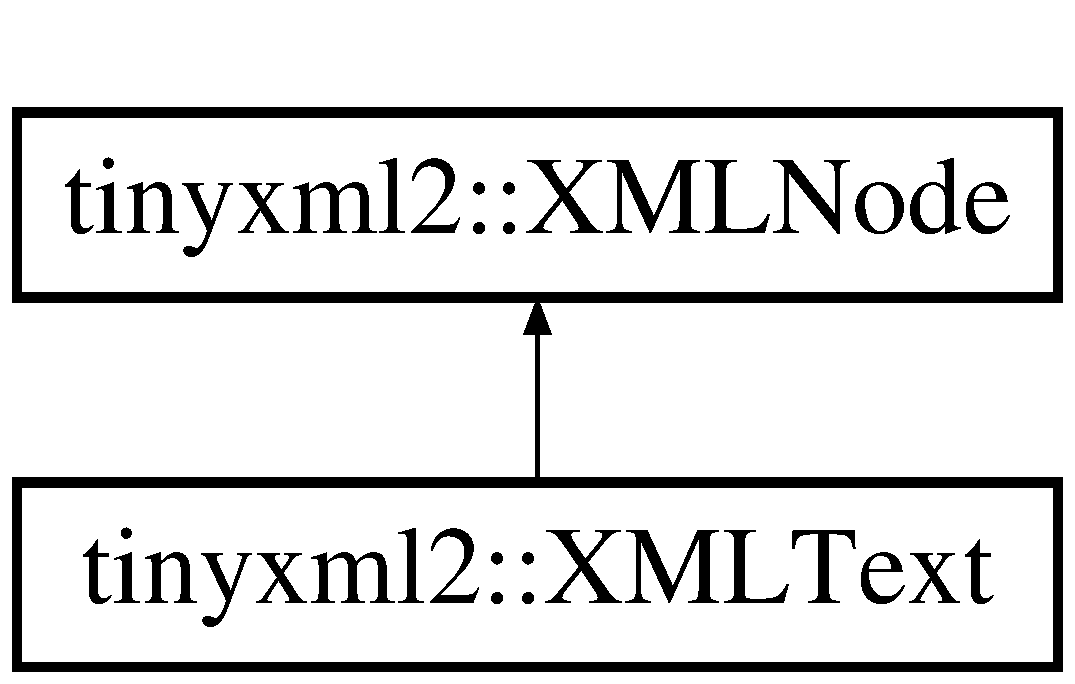
\includegraphics[height=2.000000cm]{classtinyxml2_1_1_x_m_l_text}
\end{center}
\end{figure}
\subsection*{Public Member Functions}
\begin{DoxyCompactItemize}
\item 
virtual bool \textbf{ Accept} (\textbf{ X\+M\+L\+Visitor} $\ast$visitor) const
\item 
virtual \textbf{ X\+M\+L\+Text} $\ast$ \textbf{ To\+Text} ()
\begin{DoxyCompactList}\small\item\em Safely cast to Text, or null. \end{DoxyCompactList}\item 
virtual const \textbf{ X\+M\+L\+Text} $\ast$ \textbf{ To\+Text} () const
\item 
void \textbf{ Set\+C\+Data} (bool is\+C\+Data)
\begin{DoxyCompactList}\small\item\em Declare whether this should be C\+D\+A\+TA or standard text. \end{DoxyCompactList}\item 
bool \textbf{ C\+Data} () const
\begin{DoxyCompactList}\small\item\em Returns true if this is a C\+D\+A\+TA text element. \end{DoxyCompactList}\item 
virtual \textbf{ X\+M\+L\+Node} $\ast$ \textbf{ Shallow\+Clone} (\textbf{ X\+M\+L\+Document} $\ast$document) const
\item 
virtual bool \textbf{ Shallow\+Equal} (const \textbf{ X\+M\+L\+Node} $\ast$compare) const
\end{DoxyCompactItemize}
\subsection*{Protected Member Functions}
\begin{DoxyCompactItemize}
\item 
\textbf{ X\+M\+L\+Text} (\textbf{ X\+M\+L\+Document} $\ast$doc)
\item 
virtual \textbf{ $\sim$\+X\+M\+L\+Text} ()
\item 
char $\ast$ \textbf{ Parse\+Deep} (char $\ast$p, \textbf{ Str\+Pair} $\ast$parent\+End\+Tag, int $\ast$cur\+Line\+Num\+Ptr)
\end{DoxyCompactItemize}
\subsection*{Private Member Functions}
\begin{DoxyCompactItemize}
\item 
\textbf{ X\+M\+L\+Text} (const \textbf{ X\+M\+L\+Text} \&)
\item 
\textbf{ X\+M\+L\+Text} \& \textbf{ operator=} (const \textbf{ X\+M\+L\+Text} \&)
\end{DoxyCompactItemize}
\subsection*{Private Attributes}
\begin{DoxyCompactItemize}
\item 
bool \textbf{ \+\_\+is\+C\+Data}
\end{DoxyCompactItemize}
\subsection*{Friends}
\begin{DoxyCompactItemize}
\item 
class \textbf{ X\+M\+L\+Document}
\end{DoxyCompactItemize}
\subsection*{Additional Inherited Members}


\subsection{Detailed Description}
X\+ML text.

Note that a text node can have child element nodes, for example\+: \begin{DoxyVerb}<root>This is <b>bold</b></root>
\end{DoxyVerb}


A text node can have 2 ways to output the next. \char`\"{}normal\char`\"{} output and C\+D\+A\+TA. It will default to the mode it was parsed from the X\+ML file and you generally want to leave it alone, but you can change the output mode with \doxyref{Set\+C\+Data()}{p.}{classtinyxml2_1_1_x_m_l_text_ad080357d76ab7cc59d7651249949329d} and query it with \doxyref{C\+Data()}{p.}{classtinyxml2_1_1_x_m_l_text_ac1bb5ea4166c320882d9e0ad16fd385b}. 

Definition at line 984 of file tinyxml2.\+h.



\subsection{Constructor \& Destructor Documentation}
\mbox{\label{classtinyxml2_1_1_x_m_l_text_ad9f46d70e61e5386ead93728d8b90267}} 
\index{tinyxml2::XMLText@{tinyxml2::XMLText}!XMLText@{XMLText}}
\index{XMLText@{XMLText}!tinyxml2::XMLText@{tinyxml2::XMLText}}
\subsubsection{XMLText()\hspace{0.1cm}{\footnotesize\ttfamily [1/2]}}
{\footnotesize\ttfamily tinyxml2\+::\+X\+M\+L\+Text\+::\+X\+M\+L\+Text (\begin{DoxyParamCaption}\item[{\textbf{ X\+M\+L\+Document} $\ast$}]{doc }\end{DoxyParamCaption})\hspace{0.3cm}{\ttfamily [inline]}, {\ttfamily [explicit]}, {\ttfamily [protected]}}



Definition at line 1010 of file tinyxml2.\+h.

\mbox{\label{classtinyxml2_1_1_x_m_l_text_ae9b8790d0dc13914394dbd7437c0e59d}} 
\index{tinyxml2::XMLText@{tinyxml2::XMLText}!````~XMLText@{$\sim$XMLText}}
\index{````~XMLText@{$\sim$XMLText}!tinyxml2::XMLText@{tinyxml2::XMLText}}
\subsubsection{$\sim$XMLText()}
{\footnotesize\ttfamily virtual tinyxml2\+::\+X\+M\+L\+Text\+::$\sim$\+X\+M\+L\+Text (\begin{DoxyParamCaption}{ }\end{DoxyParamCaption})\hspace{0.3cm}{\ttfamily [inline]}, {\ttfamily [protected]}, {\ttfamily [virtual]}}



Definition at line 1011 of file tinyxml2.\+h.

\mbox{\label{classtinyxml2_1_1_x_m_l_text_a002156e1f61ee6d48e5368b7cca25582}} 
\index{tinyxml2::XMLText@{tinyxml2::XMLText}!XMLText@{XMLText}}
\index{XMLText@{XMLText}!tinyxml2::XMLText@{tinyxml2::XMLText}}
\subsubsection{XMLText()\hspace{0.1cm}{\footnotesize\ttfamily [2/2]}}
{\footnotesize\ttfamily tinyxml2\+::\+X\+M\+L\+Text\+::\+X\+M\+L\+Text (\begin{DoxyParamCaption}\item[{const \textbf{ X\+M\+L\+Text} \&}]{ }\end{DoxyParamCaption})\hspace{0.3cm}{\ttfamily [private]}}



\subsection{Member Function Documentation}
\mbox{\label{classtinyxml2_1_1_x_m_l_text_a537c60d7e18fb59c45ac2737a29ac47a}} 
\index{tinyxml2::XMLText@{tinyxml2::XMLText}!Accept@{Accept}}
\index{Accept@{Accept}!tinyxml2::XMLText@{tinyxml2::XMLText}}
\subsubsection{Accept()}
{\footnotesize\ttfamily bool tinyxml2\+::\+X\+M\+L\+Text\+::\+Accept (\begin{DoxyParamCaption}\item[{\textbf{ X\+M\+L\+Visitor} $\ast$}]{visitor }\end{DoxyParamCaption}) const\hspace{0.3cm}{\ttfamily [virtual]}}

Accept a hierarchical visit of the nodes in the Tiny\+X\+M\+L-\/2 D\+OM. Every node in the X\+ML tree will be conditionally visited and the host will be called back via the \doxyref{X\+M\+L\+Visitor}{p.}{classtinyxml2_1_1_x_m_l_visitor} interface.

This is essentially a S\+AX interface for Tiny\+X\+M\+L-\/2. (Note however it doesn\textquotesingle{}t re-\/parse the X\+ML for the callbacks, so the performance of Tiny\+X\+M\+L-\/2 is unchanged by using this interface versus any other.)

The interface has been based on ideas from\+:


\begin{DoxyItemize}
\item {\texttt{ http\+://www.\+saxproject.\+org/}}
\item {\texttt{ http\+://c2.\+com/cgi/wiki?\+Hierarchical\+Visitor\+Pattern}}
\end{DoxyItemize}

Which are both good references for \char`\"{}visiting\char`\"{}.

An example of using \doxyref{Accept()}{p.}{classtinyxml2_1_1_x_m_l_text_a537c60d7e18fb59c45ac2737a29ac47a}\+: \begin{DoxyVerb}XMLPrinter printer;
tinyxmlDoc.Accept( &printer );
const char* xmlcstr = printer.CStr();
\end{DoxyVerb}
 

Implements \textbf{ tinyxml2\+::\+X\+M\+L\+Node} \doxyref{}{p.}{classtinyxml2_1_1_x_m_l_node_a81e66df0a44c67a7af17f3b77a152785}.



Definition at line 1193 of file tinyxml2.\+cpp.



References T\+I\+X\+M\+L\+A\+S\+S\+E\+RT, and tinyxml2\+::\+X\+M\+L\+Visitor\+::\+Visit().

\mbox{\label{classtinyxml2_1_1_x_m_l_text_ac1bb5ea4166c320882d9e0ad16fd385b}} 
\index{tinyxml2::XMLText@{tinyxml2::XMLText}!CData@{CData}}
\index{CData@{CData}!tinyxml2::XMLText@{tinyxml2::XMLText}}
\subsubsection{CData()}
{\footnotesize\ttfamily bool tinyxml2\+::\+X\+M\+L\+Text\+::\+C\+Data (\begin{DoxyParamCaption}{ }\end{DoxyParamCaption}) const\hspace{0.3cm}{\ttfamily [inline]}}



Returns true if this is a C\+D\+A\+TA text element. 



Definition at line 1002 of file tinyxml2.\+h.



Referenced by Parse\+Deep(), Shallow\+Clone(), and tinyxml2\+::\+X\+M\+L\+Printer\+::\+Visit().

\mbox{\label{classtinyxml2_1_1_x_m_l_text_ad8c9f398d92fa472e213b89d8483ae8f}} 
\index{tinyxml2::XMLText@{tinyxml2::XMLText}!operator=@{operator=}}
\index{operator=@{operator=}!tinyxml2::XMLText@{tinyxml2::XMLText}}
\subsubsection{operator=()}
{\footnotesize\ttfamily \textbf{ X\+M\+L\+Text}\& tinyxml2\+::\+X\+M\+L\+Text\+::operator= (\begin{DoxyParamCaption}\item[{const \textbf{ X\+M\+L\+Text} \&}]{ }\end{DoxyParamCaption})\hspace{0.3cm}{\ttfamily [private]}}

\mbox{\label{classtinyxml2_1_1_x_m_l_text_af3b93344f1183482e1683f5922ac9c68}} 
\index{tinyxml2::XMLText@{tinyxml2::XMLText}!ParseDeep@{ParseDeep}}
\index{ParseDeep@{ParseDeep}!tinyxml2::XMLText@{tinyxml2::XMLText}}
\subsubsection{ParseDeep()}
{\footnotesize\ttfamily char $\ast$ tinyxml2\+::\+X\+M\+L\+Text\+::\+Parse\+Deep (\begin{DoxyParamCaption}\item[{char $\ast$}]{p,  }\item[{\textbf{ Str\+Pair} $\ast$}]{parent\+End\+Tag,  }\item[{int $\ast$}]{cur\+Line\+Num\+Ptr }\end{DoxyParamCaption})\hspace{0.3cm}{\ttfamily [protected]}, {\ttfamily [virtual]}}



Reimplemented from \textbf{ tinyxml2\+::\+X\+M\+L\+Node} \doxyref{}{p.}{classtinyxml2_1_1_x_m_l_node_a916e498914baecbc9a1f012352ef7c69}.



Definition at line 1147 of file tinyxml2.\+cpp.



References tinyxml2\+::\+X\+M\+L\+Node\+::\+\_\+document, tinyxml2\+::\+X\+M\+L\+Node\+::\+\_\+parse\+Line\+Num, tinyxml2\+::\+X\+M\+L\+Node\+::\+\_\+value, C\+Data(), tinyxml2\+::\+C\+O\+L\+L\+A\+P\+S\+E\+\_\+\+W\+H\+I\+T\+E\+S\+P\+A\+CE, tinyxml2\+::\+Str\+Pair\+::\+N\+E\+E\+D\+S\+\_\+\+N\+E\+W\+L\+I\+N\+E\+\_\+\+N\+O\+R\+M\+A\+L\+I\+Z\+A\+T\+I\+ON, tinyxml2\+::\+Str\+Pair\+::\+N\+E\+E\+D\+S\+\_\+\+W\+H\+I\+T\+E\+S\+P\+A\+C\+E\+\_\+\+C\+O\+L\+L\+A\+P\+S\+I\+NG, tinyxml2\+::\+Str\+Pair\+::\+Parse\+Text(), tinyxml2\+::\+X\+M\+L\+Document\+::\+Process\+Entities(), tinyxml2\+::\+X\+M\+L\+Document\+::\+Set\+Error(), tinyxml2\+::\+Str\+Pair\+::\+T\+E\+X\+T\+\_\+\+E\+L\+E\+M\+E\+NT, tinyxml2\+::\+Str\+Pair\+::\+T\+E\+X\+T\+\_\+\+E\+L\+E\+M\+E\+N\+T\+\_\+\+L\+E\+A\+V\+E\+\_\+\+E\+N\+T\+I\+T\+I\+ES, tinyxml2\+::\+X\+M\+L\+Document\+::\+Whitespace\+Mode(), tinyxml2\+::\+X\+M\+L\+\_\+\+E\+R\+R\+O\+R\+\_\+\+P\+A\+R\+S\+I\+N\+G\+\_\+\+C\+D\+A\+TA, and tinyxml2\+::\+X\+M\+L\+\_\+\+E\+R\+R\+O\+R\+\_\+\+P\+A\+R\+S\+I\+N\+G\+\_\+\+T\+E\+XT.

\mbox{\label{classtinyxml2_1_1_x_m_l_text_ad080357d76ab7cc59d7651249949329d}} 
\index{tinyxml2::XMLText@{tinyxml2::XMLText}!SetCData@{SetCData}}
\index{SetCData@{SetCData}!tinyxml2::XMLText@{tinyxml2::XMLText}}
\subsubsection{SetCData()}
{\footnotesize\ttfamily void tinyxml2\+::\+X\+M\+L\+Text\+::\+Set\+C\+Data (\begin{DoxyParamCaption}\item[{bool}]{is\+C\+Data }\end{DoxyParamCaption})\hspace{0.3cm}{\ttfamily [inline]}}



Declare whether this should be C\+D\+A\+TA or standard text. 



Definition at line 998 of file tinyxml2.\+h.



Referenced by tinyxml2\+::\+X\+M\+L\+Document\+::\+Identify(), and Shallow\+Clone().

\mbox{\label{classtinyxml2_1_1_x_m_l_text_a86d265c93152726c8c6831e9594840e6}} 
\index{tinyxml2::XMLText@{tinyxml2::XMLText}!ShallowClone@{ShallowClone}}
\index{ShallowClone@{ShallowClone}!tinyxml2::XMLText@{tinyxml2::XMLText}}
\subsubsection{ShallowClone()}
{\footnotesize\ttfamily \textbf{ X\+M\+L\+Node} $\ast$ tinyxml2\+::\+X\+M\+L\+Text\+::\+Shallow\+Clone (\begin{DoxyParamCaption}\item[{\textbf{ X\+M\+L\+Document} $\ast$}]{document }\end{DoxyParamCaption}) const\hspace{0.3cm}{\ttfamily [virtual]}}

Make a copy of this node, but not its children. You may pass in a Document pointer that will be the owner of the new Node. If the \textquotesingle{}document\textquotesingle{} is null, then the node returned will be allocated from the current Document. (this-\/$>$\doxyref{Get\+Document()}{p.}{classtinyxml2_1_1_x_m_l_node_af343d1ef0b45c0020e62d784d7e67a68})

Note\+: if called on a \doxyref{X\+M\+L\+Document}{p.}{classtinyxml2_1_1_x_m_l_document}, this will return null. 

Implements \textbf{ tinyxml2\+::\+X\+M\+L\+Node} \doxyref{}{p.}{classtinyxml2_1_1_x_m_l_node_a8402cbd3129d20e9e6024bbcc0531283}.



Definition at line 1174 of file tinyxml2.\+cpp.



References tinyxml2\+::\+X\+M\+L\+Node\+::\+\_\+document, C\+Data(), tinyxml2\+::\+X\+M\+L\+Document\+::\+New\+Text(), Set\+C\+Data(), and tinyxml2\+::\+X\+M\+L\+Node\+::\+Value().

\mbox{\label{classtinyxml2_1_1_x_m_l_text_a99d8bce4dc01df889126e047f358cdfc}} 
\index{tinyxml2::XMLText@{tinyxml2::XMLText}!ShallowEqual@{ShallowEqual}}
\index{ShallowEqual@{ShallowEqual}!tinyxml2::XMLText@{tinyxml2::XMLText}}
\subsubsection{ShallowEqual()}
{\footnotesize\ttfamily bool tinyxml2\+::\+X\+M\+L\+Text\+::\+Shallow\+Equal (\begin{DoxyParamCaption}\item[{const \textbf{ X\+M\+L\+Node} $\ast$}]{compare }\end{DoxyParamCaption}) const\hspace{0.3cm}{\ttfamily [virtual]}}

Test if 2 nodes are the same, but don\textquotesingle{}t test children. The 2 nodes do not need to be in the same Document.

Note\+: if called on a \doxyref{X\+M\+L\+Document}{p.}{classtinyxml2_1_1_x_m_l_document}, this will return false. 

Implements \textbf{ tinyxml2\+::\+X\+M\+L\+Node} \doxyref{}{p.}{classtinyxml2_1_1_x_m_l_node_a7ce18b751c3ea09eac292dca264f9226}.



Definition at line 1185 of file tinyxml2.\+cpp.



References tinyxml2\+::\+X\+M\+L\+Util\+::\+String\+Equal(), T\+I\+X\+M\+L\+A\+S\+S\+E\+RT, tinyxml2\+::\+X\+M\+L\+Node\+::\+To\+Text(), and tinyxml2\+::\+X\+M\+L\+Node\+::\+Value().

\mbox{\label{classtinyxml2_1_1_x_m_l_text_ab1213b4ddebe9b17ec7e7040e9f1caf7}} 
\index{tinyxml2::XMLText@{tinyxml2::XMLText}!ToText@{ToText}}
\index{ToText@{ToText}!tinyxml2::XMLText@{tinyxml2::XMLText}}
\subsubsection{ToText()\hspace{0.1cm}{\footnotesize\ttfamily [1/2]}}
{\footnotesize\ttfamily virtual \textbf{ X\+M\+L\+Text}$\ast$ tinyxml2\+::\+X\+M\+L\+Text\+::\+To\+Text (\begin{DoxyParamCaption}{ }\end{DoxyParamCaption})\hspace{0.3cm}{\ttfamily [inline]}, {\ttfamily [virtual]}}



Safely cast to Text, or null. 



Reimplemented from \textbf{ tinyxml2\+::\+X\+M\+L\+Node} \doxyref{}{p.}{classtinyxml2_1_1_x_m_l_node_a41c55dab9162d1eb62db2008430e376b}.



Definition at line 990 of file tinyxml2.\+h.

\mbox{\label{classtinyxml2_1_1_x_m_l_text_a671ce22c7c5ef378f1ce31e6f827b9e2}} 
\index{tinyxml2::XMLText@{tinyxml2::XMLText}!ToText@{ToText}}
\index{ToText@{ToText}!tinyxml2::XMLText@{tinyxml2::XMLText}}
\subsubsection{ToText()\hspace{0.1cm}{\footnotesize\ttfamily [2/2]}}
{\footnotesize\ttfamily virtual const \textbf{ X\+M\+L\+Text}$\ast$ tinyxml2\+::\+X\+M\+L\+Text\+::\+To\+Text (\begin{DoxyParamCaption}{ }\end{DoxyParamCaption}) const\hspace{0.3cm}{\ttfamily [inline]}, {\ttfamily [virtual]}}



Reimplemented from \textbf{ tinyxml2\+::\+X\+M\+L\+Node} \doxyref{}{p.}{classtinyxml2_1_1_x_m_l_node_acb9ccc1beda27c0efcb0545683c3e7f4}.



Definition at line 993 of file tinyxml2.\+h.



\subsection{Friends And Related Function Documentation}
\mbox{\label{classtinyxml2_1_1_x_m_l_text_a4eee3bda60c60a30e4e8cd4ea91c4c6e}} 
\index{tinyxml2::XMLText@{tinyxml2::XMLText}!XMLDocument@{XMLDocument}}
\index{XMLDocument@{XMLDocument}!tinyxml2::XMLText@{tinyxml2::XMLText}}
\subsubsection{XMLDocument}
{\footnotesize\ttfamily friend class \textbf{ X\+M\+L\+Document}\hspace{0.3cm}{\ttfamily [friend]}}



Definition at line 986 of file tinyxml2.\+h.



\subsection{Member Data Documentation}
\mbox{\label{classtinyxml2_1_1_x_m_l_text_aae1a8b4117e8c8bb107900a0560d5ab5}} 
\index{tinyxml2::XMLText@{tinyxml2::XMLText}!\_isCData@{\_isCData}}
\index{\_isCData@{\_isCData}!tinyxml2::XMLText@{tinyxml2::XMLText}}
\subsubsection{\_isCData}
{\footnotesize\ttfamily bool tinyxml2\+::\+X\+M\+L\+Text\+::\+\_\+is\+C\+Data\hspace{0.3cm}{\ttfamily [private]}}



Definition at line 1016 of file tinyxml2.\+h.



The documentation for this class was generated from the following files\+:\begin{DoxyCompactItemize}
\item 
include/\textbf{ tinyxml2.\+h}\item 
src/\textbf{ tinyxml2.\+cpp}\end{DoxyCompactItemize}

\section{tinyxml2\+::X\+M\+L\+Unknown Class Reference}
\label{classtinyxml2_1_1_x_m_l_unknown}\index{tinyxml2::XMLUnknown@{tinyxml2::XMLUnknown}}


{\ttfamily \#include $<$tinyxml2.\+h$>$}

Inheritance diagram for tinyxml2\+::X\+M\+L\+Unknown\+:\begin{figure}[H]
\begin{center}
\leavevmode
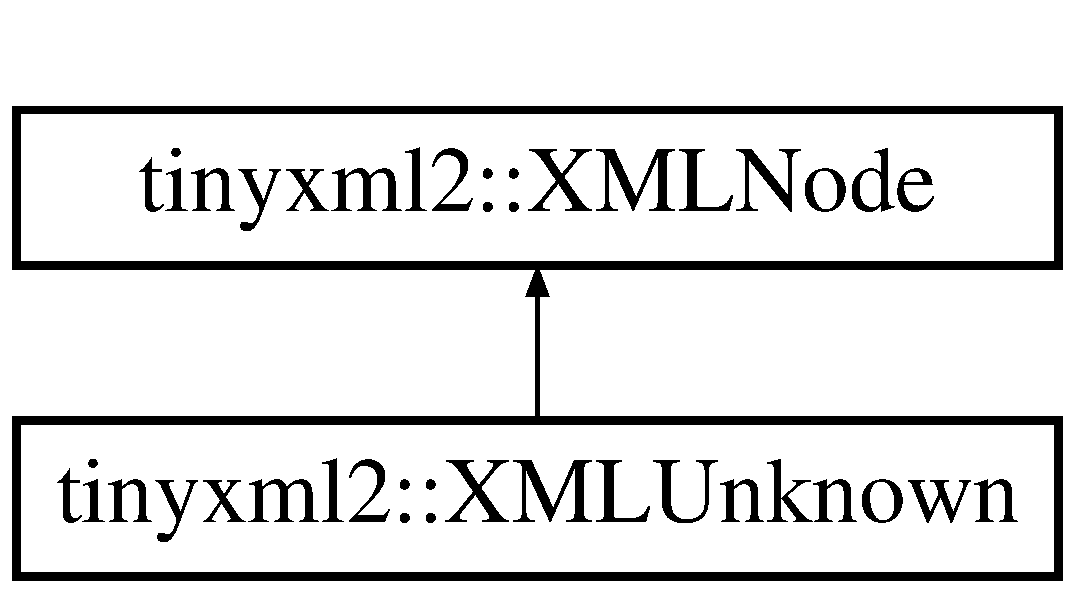
\includegraphics[height=2.000000cm]{classtinyxml2_1_1_x_m_l_unknown}
\end{center}
\end{figure}
\subsection*{Public Member Functions}
\begin{DoxyCompactItemize}
\item 
virtual \textbf{ X\+M\+L\+Unknown} $\ast$ \textbf{ To\+Unknown} ()
\begin{DoxyCompactList}\small\item\em Safely cast to an Unknown, or null. \end{DoxyCompactList}\item 
virtual const \textbf{ X\+M\+L\+Unknown} $\ast$ \textbf{ To\+Unknown} () const
\item 
virtual bool \textbf{ Accept} (\textbf{ X\+M\+L\+Visitor} $\ast$visitor) const
\item 
virtual \textbf{ X\+M\+L\+Node} $\ast$ \textbf{ Shallow\+Clone} (\textbf{ X\+M\+L\+Document} $\ast$document) const
\item 
virtual bool \textbf{ Shallow\+Equal} (const \textbf{ X\+M\+L\+Node} $\ast$compare) const
\end{DoxyCompactItemize}
\subsection*{Protected Member Functions}
\begin{DoxyCompactItemize}
\item 
\textbf{ X\+M\+L\+Unknown} (\textbf{ X\+M\+L\+Document} $\ast$doc)
\item 
virtual \textbf{ $\sim$\+X\+M\+L\+Unknown} ()
\item 
char $\ast$ \textbf{ Parse\+Deep} (char $\ast$p, \textbf{ Str\+Pair} $\ast$parent\+End\+Tag, int $\ast$cur\+Line\+Num\+Ptr)
\end{DoxyCompactItemize}
\subsection*{Private Member Functions}
\begin{DoxyCompactItemize}
\item 
\textbf{ X\+M\+L\+Unknown} (const \textbf{ X\+M\+L\+Unknown} \&)
\item 
\textbf{ X\+M\+L\+Unknown} \& \textbf{ operator=} (const \textbf{ X\+M\+L\+Unknown} \&)
\end{DoxyCompactItemize}
\subsection*{Friends}
\begin{DoxyCompactItemize}
\item 
class \textbf{ X\+M\+L\+Document}
\end{DoxyCompactItemize}
\subsection*{Additional Inherited Members}


\subsection{Detailed Description}
Any tag that Tiny\+X\+M\+L-\/2 doesn\textquotesingle{}t recognize is saved as an unknown. It is a tag of text, but should not be modified. It will be written back to the X\+ML, unchanged, when the file is saved.

D\+TD tags get thrown into X\+M\+L\+Unknowns. 

Definition at line 1098 of file tinyxml2.\+h.



\subsection{Constructor \& Destructor Documentation}
\mbox{\label{classtinyxml2_1_1_x_m_l_unknown_a9391eb679598d50baba424e6f1aa367b}} 
\index{tinyxml2::XMLUnknown@{tinyxml2::XMLUnknown}!XMLUnknown@{XMLUnknown}}
\index{XMLUnknown@{XMLUnknown}!tinyxml2::XMLUnknown@{tinyxml2::XMLUnknown}}
\subsubsection{XMLUnknown()\hspace{0.1cm}{\footnotesize\ttfamily [1/2]}}
{\footnotesize\ttfamily tinyxml2\+::\+X\+M\+L\+Unknown\+::\+X\+M\+L\+Unknown (\begin{DoxyParamCaption}\item[{\textbf{ X\+M\+L\+Document} $\ast$}]{doc }\end{DoxyParamCaption})\hspace{0.3cm}{\ttfamily [explicit]}, {\ttfamily [protected]}}



Definition at line 1299 of file tinyxml2.\+cpp.

\mbox{\label{classtinyxml2_1_1_x_m_l_unknown_a86fcd722ca173a7f385bafafa879f26e}} 
\index{tinyxml2::XMLUnknown@{tinyxml2::XMLUnknown}!````~XMLUnknown@{$\sim$XMLUnknown}}
\index{````~XMLUnknown@{$\sim$XMLUnknown}!tinyxml2::XMLUnknown@{tinyxml2::XMLUnknown}}
\subsubsection{$\sim$XMLUnknown()}
{\footnotesize\ttfamily tinyxml2\+::\+X\+M\+L\+Unknown\+::$\sim$\+X\+M\+L\+Unknown (\begin{DoxyParamCaption}{ }\end{DoxyParamCaption})\hspace{0.3cm}{\ttfamily [protected]}, {\ttfamily [virtual]}}



Definition at line 1304 of file tinyxml2.\+cpp.

\mbox{\label{classtinyxml2_1_1_x_m_l_unknown_aab31a93c95a7cedc9597cea7caffa73f}} 
\index{tinyxml2::XMLUnknown@{tinyxml2::XMLUnknown}!XMLUnknown@{XMLUnknown}}
\index{XMLUnknown@{XMLUnknown}!tinyxml2::XMLUnknown@{tinyxml2::XMLUnknown}}
\subsubsection{XMLUnknown()\hspace{0.1cm}{\footnotesize\ttfamily [2/2]}}
{\footnotesize\ttfamily tinyxml2\+::\+X\+M\+L\+Unknown\+::\+X\+M\+L\+Unknown (\begin{DoxyParamCaption}\item[{const \textbf{ X\+M\+L\+Unknown} \&}]{ }\end{DoxyParamCaption})\hspace{0.3cm}{\ttfamily [private]}}



\subsection{Member Function Documentation}
\mbox{\label{classtinyxml2_1_1_x_m_l_unknown_a8a06b8c82117ca969a432e17a46830fc}} 
\index{tinyxml2::XMLUnknown@{tinyxml2::XMLUnknown}!Accept@{Accept}}
\index{Accept@{Accept}!tinyxml2::XMLUnknown@{tinyxml2::XMLUnknown}}
\subsubsection{Accept()}
{\footnotesize\ttfamily bool tinyxml2\+::\+X\+M\+L\+Unknown\+::\+Accept (\begin{DoxyParamCaption}\item[{\textbf{ X\+M\+L\+Visitor} $\ast$}]{visitor }\end{DoxyParamCaption}) const\hspace{0.3cm}{\ttfamily [virtual]}}

Accept a hierarchical visit of the nodes in the Tiny\+X\+M\+L-\/2 D\+OM. Every node in the X\+ML tree will be conditionally visited and the host will be called back via the \doxyref{X\+M\+L\+Visitor}{p.}{classtinyxml2_1_1_x_m_l_visitor} interface.

This is essentially a S\+AX interface for Tiny\+X\+M\+L-\/2. (Note however it doesn\textquotesingle{}t re-\/parse the X\+ML for the callbacks, so the performance of Tiny\+X\+M\+L-\/2 is unchanged by using this interface versus any other.)

The interface has been based on ideas from\+:


\begin{DoxyItemize}
\item {\texttt{ http\+://www.\+saxproject.\+org/}}
\item {\texttt{ http\+://c2.\+com/cgi/wiki?\+Hierarchical\+Visitor\+Pattern}}
\end{DoxyItemize}

Which are both good references for \char`\"{}visiting\char`\"{}.

An example of using \doxyref{Accept()}{p.}{classtinyxml2_1_1_x_m_l_unknown_a8a06b8c82117ca969a432e17a46830fc}\+: \begin{DoxyVerb}XMLPrinter printer;
tinyxmlDoc.Accept( &printer );
const char* xmlcstr = printer.CStr();
\end{DoxyVerb}
 

Implements \textbf{ tinyxml2\+::\+X\+M\+L\+Node} \doxyref{}{p.}{classtinyxml2_1_1_x_m_l_node_a81e66df0a44c67a7af17f3b77a152785}.



Definition at line 1338 of file tinyxml2.\+cpp.



References T\+I\+X\+M\+L\+A\+S\+S\+E\+RT, and tinyxml2\+::\+X\+M\+L\+Visitor\+::\+Visit().

\mbox{\label{classtinyxml2_1_1_x_m_l_unknown_a6137d5611db42c35de3d869f66555e5b}} 
\index{tinyxml2::XMLUnknown@{tinyxml2::XMLUnknown}!operator=@{operator=}}
\index{operator=@{operator=}!tinyxml2::XMLUnknown@{tinyxml2::XMLUnknown}}
\subsubsection{operator=()}
{\footnotesize\ttfamily \textbf{ X\+M\+L\+Unknown}\& tinyxml2\+::\+X\+M\+L\+Unknown\+::operator= (\begin{DoxyParamCaption}\item[{const \textbf{ X\+M\+L\+Unknown} \&}]{ }\end{DoxyParamCaption})\hspace{0.3cm}{\ttfamily [private]}}

\mbox{\label{classtinyxml2_1_1_x_m_l_unknown_aefc332cc1e6e25736f364d1e5eeb31fe}} 
\index{tinyxml2::XMLUnknown@{tinyxml2::XMLUnknown}!ParseDeep@{ParseDeep}}
\index{ParseDeep@{ParseDeep}!tinyxml2::XMLUnknown@{tinyxml2::XMLUnknown}}
\subsubsection{ParseDeep()}
{\footnotesize\ttfamily char $\ast$ tinyxml2\+::\+X\+M\+L\+Unknown\+::\+Parse\+Deep (\begin{DoxyParamCaption}\item[{char $\ast$}]{p,  }\item[{\textbf{ Str\+Pair} $\ast$}]{parent\+End\+Tag,  }\item[{int $\ast$}]{cur\+Line\+Num\+Ptr }\end{DoxyParamCaption})\hspace{0.3cm}{\ttfamily [protected]}, {\ttfamily [virtual]}}



Reimplemented from \textbf{ tinyxml2\+::\+X\+M\+L\+Node} \doxyref{}{p.}{classtinyxml2_1_1_x_m_l_node_a916e498914baecbc9a1f012352ef7c69}.



Definition at line 1309 of file tinyxml2.\+cpp.



References tinyxml2\+::\+X\+M\+L\+Node\+::\+\_\+document, tinyxml2\+::\+X\+M\+L\+Node\+::\+\_\+parse\+Line\+Num, tinyxml2\+::\+X\+M\+L\+Node\+::\+\_\+value, tinyxml2\+::\+Str\+Pair\+::\+N\+E\+E\+D\+S\+\_\+\+N\+E\+W\+L\+I\+N\+E\+\_\+\+N\+O\+R\+M\+A\+L\+I\+Z\+A\+T\+I\+ON, tinyxml2\+::\+Str\+Pair\+::\+Parse\+Text(), tinyxml2\+::\+X\+M\+L\+Document\+::\+Set\+Error(), and tinyxml2\+::\+X\+M\+L\+\_\+\+E\+R\+R\+O\+R\+\_\+\+P\+A\+R\+S\+I\+N\+G\+\_\+\+U\+N\+K\+N\+O\+WN.

\mbox{\label{classtinyxml2_1_1_x_m_l_unknown_ab73b48b819aa4b2ef3815dc2d7d20d5f}} 
\index{tinyxml2::XMLUnknown@{tinyxml2::XMLUnknown}!ShallowClone@{ShallowClone}}
\index{ShallowClone@{ShallowClone}!tinyxml2::XMLUnknown@{tinyxml2::XMLUnknown}}
\subsubsection{ShallowClone()}
{\footnotesize\ttfamily \textbf{ X\+M\+L\+Node} $\ast$ tinyxml2\+::\+X\+M\+L\+Unknown\+::\+Shallow\+Clone (\begin{DoxyParamCaption}\item[{\textbf{ X\+M\+L\+Document} $\ast$}]{document }\end{DoxyParamCaption}) const\hspace{0.3cm}{\ttfamily [virtual]}}

Make a copy of this node, but not its children. You may pass in a Document pointer that will be the owner of the new Node. If the \textquotesingle{}document\textquotesingle{} is null, then the node returned will be allocated from the current Document. (this-\/$>$\doxyref{Get\+Document()}{p.}{classtinyxml2_1_1_x_m_l_node_af343d1ef0b45c0020e62d784d7e67a68})

Note\+: if called on a \doxyref{X\+M\+L\+Document}{p.}{classtinyxml2_1_1_x_m_l_document}, this will return null. 

Implements \textbf{ tinyxml2\+::\+X\+M\+L\+Node} \doxyref{}{p.}{classtinyxml2_1_1_x_m_l_node_a8402cbd3129d20e9e6024bbcc0531283}.



Definition at line 1320 of file tinyxml2.\+cpp.



References tinyxml2\+::\+X\+M\+L\+Node\+::\+\_\+document, tinyxml2\+::\+X\+M\+L\+Document\+::\+New\+Unknown(), and tinyxml2\+::\+X\+M\+L\+Node\+::\+Value().

\mbox{\label{classtinyxml2_1_1_x_m_l_unknown_ac46767cd721d666e690a6231dfb618d1}} 
\index{tinyxml2::XMLUnknown@{tinyxml2::XMLUnknown}!ShallowEqual@{ShallowEqual}}
\index{ShallowEqual@{ShallowEqual}!tinyxml2::XMLUnknown@{tinyxml2::XMLUnknown}}
\subsubsection{ShallowEqual()}
{\footnotesize\ttfamily bool tinyxml2\+::\+X\+M\+L\+Unknown\+::\+Shallow\+Equal (\begin{DoxyParamCaption}\item[{const \textbf{ X\+M\+L\+Node} $\ast$}]{compare }\end{DoxyParamCaption}) const\hspace{0.3cm}{\ttfamily [virtual]}}

Test if 2 nodes are the same, but don\textquotesingle{}t test children. The 2 nodes do not need to be in the same Document.

Note\+: if called on a \doxyref{X\+M\+L\+Document}{p.}{classtinyxml2_1_1_x_m_l_document}, this will return false. 

Implements \textbf{ tinyxml2\+::\+X\+M\+L\+Node} \doxyref{}{p.}{classtinyxml2_1_1_x_m_l_node_a7ce18b751c3ea09eac292dca264f9226}.



Definition at line 1330 of file tinyxml2.\+cpp.



References tinyxml2\+::\+X\+M\+L\+Util\+::\+String\+Equal(), T\+I\+X\+M\+L\+A\+S\+S\+E\+RT, tinyxml2\+::\+X\+M\+L\+Node\+::\+To\+Unknown(), and tinyxml2\+::\+X\+M\+L\+Node\+::\+Value().

\mbox{\label{classtinyxml2_1_1_x_m_l_unknown_af4374856421921cad578c8affae872b6}} 
\index{tinyxml2::XMLUnknown@{tinyxml2::XMLUnknown}!ToUnknown@{ToUnknown}}
\index{ToUnknown@{ToUnknown}!tinyxml2::XMLUnknown@{tinyxml2::XMLUnknown}}
\subsubsection{ToUnknown()\hspace{0.1cm}{\footnotesize\ttfamily [1/2]}}
{\footnotesize\ttfamily virtual \textbf{ X\+M\+L\+Unknown}$\ast$ tinyxml2\+::\+X\+M\+L\+Unknown\+::\+To\+Unknown (\begin{DoxyParamCaption}{ }\end{DoxyParamCaption})\hspace{0.3cm}{\ttfamily [inline]}, {\ttfamily [virtual]}}



Safely cast to an Unknown, or null. 



Reimplemented from \textbf{ tinyxml2\+::\+X\+M\+L\+Node} \doxyref{}{p.}{classtinyxml2_1_1_x_m_l_node_a8675a74aa0ada6eccab0c77ef3e5b9bd}.



Definition at line 1102 of file tinyxml2.\+h.

\mbox{\label{classtinyxml2_1_1_x_m_l_unknown_a61b342b4f295cded1dc2f4402e97f07e}} 
\index{tinyxml2::XMLUnknown@{tinyxml2::XMLUnknown}!ToUnknown@{ToUnknown}}
\index{ToUnknown@{ToUnknown}!tinyxml2::XMLUnknown@{tinyxml2::XMLUnknown}}
\subsubsection{ToUnknown()\hspace{0.1cm}{\footnotesize\ttfamily [2/2]}}
{\footnotesize\ttfamily virtual const \textbf{ X\+M\+L\+Unknown}$\ast$ tinyxml2\+::\+X\+M\+L\+Unknown\+::\+To\+Unknown (\begin{DoxyParamCaption}{ }\end{DoxyParamCaption}) const\hspace{0.3cm}{\ttfamily [inline]}, {\ttfamily [virtual]}}



Reimplemented from \textbf{ tinyxml2\+::\+X\+M\+L\+Node} \doxyref{}{p.}{classtinyxml2_1_1_x_m_l_node_af29ffd6cbe609b6fa04a705256150408}.



Definition at line 1105 of file tinyxml2.\+h.



\subsection{Friends And Related Function Documentation}
\mbox{\label{classtinyxml2_1_1_x_m_l_unknown_a4eee3bda60c60a30e4e8cd4ea91c4c6e}} 
\index{tinyxml2::XMLUnknown@{tinyxml2::XMLUnknown}!XMLDocument@{XMLDocument}}
\index{XMLDocument@{XMLDocument}!tinyxml2::XMLUnknown@{tinyxml2::XMLUnknown}}
\subsubsection{XMLDocument}
{\footnotesize\ttfamily friend class \textbf{ X\+M\+L\+Document}\hspace{0.3cm}{\ttfamily [friend]}}



Definition at line 1100 of file tinyxml2.\+h.



The documentation for this class was generated from the following files\+:\begin{DoxyCompactItemize}
\item 
include/\textbf{ tinyxml2.\+h}\item 
src/\textbf{ tinyxml2.\+cpp}\end{DoxyCompactItemize}

\section{tinyxml2\+:\+:X\+M\+L\+Util Class Reference}
\label{classtinyxml2_1_1_x_m_l_util}\index{tinyxml2\+::\+X\+M\+L\+Util@{tinyxml2\+::\+X\+M\+L\+Util}}


{\ttfamily \#include $<$tinyxml2.\+h$>$}

\subsection*{Static Public Member Functions}
\begin{DoxyCompactItemize}
\item 
static const char $\ast$ \textbf{ Skip\+White\+Space} (const char $\ast$p, int $\ast$cur\+Line\+Num\+Ptr)
\item 
static char $\ast$ \textbf{ Skip\+White\+Space} (char $\ast$p, int $\ast$cur\+Line\+Num\+Ptr)
\item 
static bool \textbf{ Is\+White\+Space} (char p)
\item 
static bool \textbf{ Is\+Name\+Start\+Char} (unsigned char ch)
\item 
static bool \textbf{ Is\+Name\+Char} (unsigned char ch)
\item 
static bool \textbf{ String\+Equal} (const char $\ast$p, const char $\ast$q, int n\+Char=I\+N\+T\+\_\+\+M\+AX)
\item 
static bool \textbf{ Is\+U\+T\+F8\+Continuation} (char p)
\item 
static const char $\ast$ \textbf{ Read\+B\+OM} (const char $\ast$p, bool $\ast$has\+B\+OM)
\item 
static const char $\ast$ \textbf{ Get\+Character\+Ref} (const char $\ast$p, char $\ast$value, int $\ast$length)
\item 
static void \textbf{ Convert\+U\+T\+F32\+To\+U\+T\+F8} (unsigned long input, char $\ast$output, int $\ast$length)
\item 
static void \textbf{ To\+Str} (int v, char $\ast$buffer, int buffer\+Size)
\item 
static void \textbf{ To\+Str} (unsigned v, char $\ast$buffer, int buffer\+Size)
\item 
static void \textbf{ To\+Str} (bool v, char $\ast$buffer, int buffer\+Size)
\item 
static void \textbf{ To\+Str} (float v, char $\ast$buffer, int buffer\+Size)
\item 
static void \textbf{ To\+Str} (double v, char $\ast$buffer, int buffer\+Size)
\item 
static void \textbf{ To\+Str} (int64\+\_\+t v, char $\ast$buffer, int buffer\+Size)
\item 
static bool \textbf{ To\+Int} (const char $\ast$str, int $\ast$value)
\item 
static bool \textbf{ To\+Unsigned} (const char $\ast$str, unsigned $\ast$value)
\item 
static bool \textbf{ To\+Bool} (const char $\ast$str, bool $\ast$value)
\item 
static bool \textbf{ To\+Float} (const char $\ast$str, float $\ast$value)
\item 
static bool \textbf{ To\+Double} (const char $\ast$str, double $\ast$value)
\item 
static bool \textbf{ To\+Int64} (const char $\ast$str, int64\+\_\+t $\ast$value)
\item 
static void \textbf{ Set\+Bool\+Serialization} (const char $\ast$write\+True, const char $\ast$write\+False)
\end{DoxyCompactItemize}
\subsection*{Static Private Attributes}
\begin{DoxyCompactItemize}
\item 
static const char $\ast$ \textbf{ write\+Bool\+True} = \char`\"{}true\char`\"{}
\item 
static const char $\ast$ \textbf{ write\+Bool\+False} = \char`\"{}false\char`\"{}
\end{DoxyCompactItemize}


\subsection{Detailed Description}


Definition at line 550 of file tinyxml2.\+h.



\subsection{Member Function Documentation}
\mbox{\label{classtinyxml2_1_1_x_m_l_util_a31c00d5c5dfb38382de1dfcaf4be3595}} 
\index{tinyxml2\+::\+X\+M\+L\+Util@{tinyxml2\+::\+X\+M\+L\+Util}!Convert\+U\+T\+F32\+To\+U\+T\+F8@{Convert\+U\+T\+F32\+To\+U\+T\+F8}}
\index{Convert\+U\+T\+F32\+To\+U\+T\+F8@{Convert\+U\+T\+F32\+To\+U\+T\+F8}!tinyxml2\+::\+X\+M\+L\+Util@{tinyxml2\+::\+X\+M\+L\+Util}}
\subsubsection{Convert\+U\+T\+F32\+To\+U\+T\+F8()}
{\footnotesize\ttfamily void tinyxml2\+::\+X\+M\+L\+Util\+::\+Convert\+U\+T\+F32\+To\+U\+T\+F8 (\begin{DoxyParamCaption}\item[{unsigned long}]{input,  }\item[{char $\ast$}]{output,  }\item[{int $\ast$}]{length }\end{DoxyParamCaption})\hspace{0.3cm}{\ttfamily [static]}}



Definition at line 403 of file tinyxml2.\+cpp.



References tinyxml2\+::\+Entity\+::length, and T\+I\+X\+M\+L\+A\+S\+S\+E\+RT.

\mbox{\label{classtinyxml2_1_1_x_m_l_util_a5a96e5144a8d693dc4bcd783d9964648}} 
\index{tinyxml2\+::\+X\+M\+L\+Util@{tinyxml2\+::\+X\+M\+L\+Util}!Get\+Character\+Ref@{Get\+Character\+Ref}}
\index{Get\+Character\+Ref@{Get\+Character\+Ref}!tinyxml2\+::\+X\+M\+L\+Util@{tinyxml2\+::\+X\+M\+L\+Util}}
\subsubsection{Get\+Character\+Ref()}
{\footnotesize\ttfamily const char $\ast$ tinyxml2\+::\+X\+M\+L\+Util\+::\+Get\+Character\+Ref (\begin{DoxyParamCaption}\item[{const char $\ast$}]{p,  }\item[{char $\ast$}]{value,  }\item[{int $\ast$}]{length }\end{DoxyParamCaption})\hspace{0.3cm}{\ttfamily [static]}}



Definition at line 456 of file tinyxml2.\+cpp.



References T\+I\+X\+M\+L\+A\+S\+S\+E\+RT.

\mbox{\label{classtinyxml2_1_1_x_m_l_util_a04b17341538fa11752f24b4301d19485}} 
\index{tinyxml2\+::\+X\+M\+L\+Util@{tinyxml2\+::\+X\+M\+L\+Util}!Is\+Name\+Char@{Is\+Name\+Char}}
\index{Is\+Name\+Char@{Is\+Name\+Char}!tinyxml2\+::\+X\+M\+L\+Util@{tinyxml2\+::\+X\+M\+L\+Util}}
\subsubsection{Is\+Name\+Char()}
{\footnotesize\ttfamily static bool tinyxml2\+::\+X\+M\+L\+Util\+::\+Is\+Name\+Char (\begin{DoxyParamCaption}\item[{unsigned char}]{ch }\end{DoxyParamCaption})\hspace{0.3cm}{\ttfamily [inline]}, {\ttfamily [static]}}



Definition at line 586 of file tinyxml2.\+h.



Referenced by tinyxml2\+::\+Str\+Pair\+::\+Parse\+Name().

\mbox{\label{classtinyxml2_1_1_x_m_l_util_abe106a69ac4d942a4381a4d9dfd0e0bd}} 
\index{tinyxml2\+::\+X\+M\+L\+Util@{tinyxml2\+::\+X\+M\+L\+Util}!Is\+Name\+Start\+Char@{Is\+Name\+Start\+Char}}
\index{Is\+Name\+Start\+Char@{Is\+Name\+Start\+Char}!tinyxml2\+::\+X\+M\+L\+Util@{tinyxml2\+::\+X\+M\+L\+Util}}
\subsubsection{Is\+Name\+Start\+Char()}
{\footnotesize\ttfamily static bool tinyxml2\+::\+X\+M\+L\+Util\+::\+Is\+Name\+Start\+Char (\begin{DoxyParamCaption}\item[{unsigned char}]{ch }\end{DoxyParamCaption})\hspace{0.3cm}{\ttfamily [inline]}, {\ttfamily [static]}}



Definition at line 575 of file tinyxml2.\+h.



Referenced by tinyxml2\+::\+X\+M\+L\+Element\+::\+Parse\+Attributes(), and tinyxml2\+::\+Str\+Pair\+::\+Parse\+Name().

\mbox{\label{classtinyxml2_1_1_x_m_l_util_ad7fd82e0fe610d73ef7bf9f359f104a3}} 
\index{tinyxml2\+::\+X\+M\+L\+Util@{tinyxml2\+::\+X\+M\+L\+Util}!Is\+U\+T\+F8\+Continuation@{Is\+U\+T\+F8\+Continuation}}
\index{Is\+U\+T\+F8\+Continuation@{Is\+U\+T\+F8\+Continuation}!tinyxml2\+::\+X\+M\+L\+Util@{tinyxml2\+::\+X\+M\+L\+Util}}
\subsubsection{Is\+U\+T\+F8\+Continuation()}
{\footnotesize\ttfamily static bool tinyxml2\+::\+X\+M\+L\+Util\+::\+Is\+U\+T\+F8\+Continuation (\begin{DoxyParamCaption}\item[{char}]{p }\end{DoxyParamCaption})\hspace{0.3cm}{\ttfamily [inline]}, {\ttfamily [static]}}



Definition at line 603 of file tinyxml2.\+h.

\mbox{\label{classtinyxml2_1_1_x_m_l_util_a357ec3af8fc433d19023a815f45e8e33}} 
\index{tinyxml2\+::\+X\+M\+L\+Util@{tinyxml2\+::\+X\+M\+L\+Util}!Is\+White\+Space@{Is\+White\+Space}}
\index{Is\+White\+Space@{Is\+White\+Space}!tinyxml2\+::\+X\+M\+L\+Util@{tinyxml2\+::\+X\+M\+L\+Util}}
\subsubsection{Is\+White\+Space()}
{\footnotesize\ttfamily static bool tinyxml2\+::\+X\+M\+L\+Util\+::\+Is\+White\+Space (\begin{DoxyParamCaption}\item[{char}]{p }\end{DoxyParamCaption})\hspace{0.3cm}{\ttfamily [inline]}, {\ttfamily [static]}}



Definition at line 571 of file tinyxml2.\+h.



Referenced by tinyxml2\+::\+Str\+Pair\+::\+Collapse\+Whitespace().

\mbox{\label{classtinyxml2_1_1_x_m_l_util_ae9bcb2bc3cd6475fdc644c8c17790555}} 
\index{tinyxml2\+::\+X\+M\+L\+Util@{tinyxml2\+::\+X\+M\+L\+Util}!Read\+B\+OM@{Read\+B\+OM}}
\index{Read\+B\+OM@{Read\+B\+OM}!tinyxml2\+::\+X\+M\+L\+Util@{tinyxml2\+::\+X\+M\+L\+Util}}
\subsubsection{Read\+B\+O\+M()}
{\footnotesize\ttfamily const char $\ast$ tinyxml2\+::\+X\+M\+L\+Util\+::\+Read\+B\+OM (\begin{DoxyParamCaption}\item[{const char $\ast$}]{p,  }\item[{bool $\ast$}]{has\+B\+OM }\end{DoxyParamCaption})\hspace{0.3cm}{\ttfamily [static]}}



Definition at line 385 of file tinyxml2.\+cpp.



References T\+I\+X\+M\+L\+A\+S\+S\+E\+RT.



Referenced by tinyxml2\+::\+X\+M\+L\+Document\+::\+Parse().

\mbox{\label{classtinyxml2_1_1_x_m_l_util_af98a6a80dbeec4679366c1aba4c5b747}} 
\index{tinyxml2\+::\+X\+M\+L\+Util@{tinyxml2\+::\+X\+M\+L\+Util}!Set\+Bool\+Serialization@{Set\+Bool\+Serialization}}
\index{Set\+Bool\+Serialization@{Set\+Bool\+Serialization}!tinyxml2\+::\+X\+M\+L\+Util@{tinyxml2\+::\+X\+M\+L\+Util}}
\subsubsection{Set\+Bool\+Serialization()}
{\footnotesize\ttfamily void tinyxml2\+::\+X\+M\+L\+Util\+::\+Set\+Bool\+Serialization (\begin{DoxyParamCaption}\item[{const char $\ast$}]{write\+True,  }\item[{const char $\ast$}]{write\+False }\end{DoxyParamCaption})\hspace{0.3cm}{\ttfamily [static]}}



Definition at line 375 of file tinyxml2.\+cpp.

\mbox{\label{classtinyxml2_1_1_x_m_l_util_ab626a194b3523a5ba8b9dbaa2a165202}} 
\index{tinyxml2\+::\+X\+M\+L\+Util@{tinyxml2\+::\+X\+M\+L\+Util}!Skip\+White\+Space@{Skip\+White\+Space}}
\index{Skip\+White\+Space@{Skip\+White\+Space}!tinyxml2\+::\+X\+M\+L\+Util@{tinyxml2\+::\+X\+M\+L\+Util}}
\subsubsection{Skip\+White\+Space()\hspace{0.1cm}{\footnotesize\ttfamily [1/2]}}
{\footnotesize\ttfamily static const char$\ast$ tinyxml2\+::\+X\+M\+L\+Util\+::\+Skip\+White\+Space (\begin{DoxyParamCaption}\item[{const char $\ast$}]{p,  }\item[{int $\ast$}]{cur\+Line\+Num\+Ptr }\end{DoxyParamCaption})\hspace{0.3cm}{\ttfamily [inline]}, {\ttfamily [static]}}



Definition at line 553 of file tinyxml2.\+h.



References T\+I\+X\+M\+L\+A\+S\+S\+E\+RT.



Referenced by tinyxml2\+::\+Str\+Pair\+::\+Collapse\+Whitespace(), tinyxml2\+::\+X\+M\+L\+Document\+::\+Identify(), tinyxml2\+::\+X\+M\+L\+Document\+::\+Parse(), tinyxml2\+::\+X\+M\+L\+Element\+::\+Parse\+Attributes(), tinyxml2\+::\+X\+M\+L\+Attribute\+::\+Parse\+Deep(), and tinyxml2\+::\+X\+M\+L\+Element\+::\+Parse\+Deep().

\mbox{\label{classtinyxml2_1_1_x_m_l_util_abb6cb3e71f88efca82cb7157367fd91e}} 
\index{tinyxml2\+::\+X\+M\+L\+Util@{tinyxml2\+::\+X\+M\+L\+Util}!Skip\+White\+Space@{Skip\+White\+Space}}
\index{Skip\+White\+Space@{Skip\+White\+Space}!tinyxml2\+::\+X\+M\+L\+Util@{tinyxml2\+::\+X\+M\+L\+Util}}
\subsubsection{Skip\+White\+Space()\hspace{0.1cm}{\footnotesize\ttfamily [2/2]}}
{\footnotesize\ttfamily static char$\ast$ tinyxml2\+::\+X\+M\+L\+Util\+::\+Skip\+White\+Space (\begin{DoxyParamCaption}\item[{char $\ast$}]{p,  }\item[{int $\ast$}]{cur\+Line\+Num\+Ptr }\end{DoxyParamCaption})\hspace{0.3cm}{\ttfamily [inline]}, {\ttfamily [static]}}



Definition at line 565 of file tinyxml2.\+h.

\mbox{\label{classtinyxml2_1_1_x_m_l_util_acfcd287cacfd2533e1bc9ea4dfb56602}} 
\index{tinyxml2\+::\+X\+M\+L\+Util@{tinyxml2\+::\+X\+M\+L\+Util}!String\+Equal@{String\+Equal}}
\index{String\+Equal@{String\+Equal}!tinyxml2\+::\+X\+M\+L\+Util@{tinyxml2\+::\+X\+M\+L\+Util}}
\subsubsection{String\+Equal()}
{\footnotesize\ttfamily static bool tinyxml2\+::\+X\+M\+L\+Util\+::\+String\+Equal (\begin{DoxyParamCaption}\item[{const char $\ast$}]{p,  }\item[{const char $\ast$}]{q,  }\item[{int}]{n\+Char = {\ttfamily INT\+\_\+MAX} }\end{DoxyParamCaption})\hspace{0.3cm}{\ttfamily [inline]}, {\ttfamily [static]}}



Definition at line 593 of file tinyxml2.\+h.



References T\+I\+X\+M\+L\+A\+S\+S\+E\+RT.



Referenced by tinyxml2\+::\+X\+M\+L\+Element\+::\+Attribute(), tinyxml2\+::\+X\+M\+L\+Element\+::\+Delete\+Attribute(), tinyxml2\+::\+X\+M\+L\+Element\+::\+Find\+Attribute(), tinyxml2\+::\+X\+M\+L\+Element\+::\+Find\+Or\+Create\+Attribute(), tinyxml2\+::\+X\+M\+L\+Document\+::\+Identify(), tinyxml2\+::\+X\+M\+L\+Node\+::\+Parse\+Deep(), tinyxml2\+::\+X\+M\+L\+Text\+::\+Shallow\+Equal(), tinyxml2\+::\+X\+M\+L\+Comment\+::\+Shallow\+Equal(), tinyxml2\+::\+X\+M\+L\+Declaration\+::\+Shallow\+Equal(), tinyxml2\+::\+X\+M\+L\+Unknown\+::\+Shallow\+Equal(), tinyxml2\+::\+X\+M\+L\+Element\+::\+Shallow\+Equal(), and tinyxml2\+::\+X\+M\+L\+Node\+::\+To\+Element\+With\+Name().

\mbox{\label{classtinyxml2_1_1_x_m_l_util_ae5b03e0a1ca5d42052a7ac540f7aa12a}} 
\index{tinyxml2\+::\+X\+M\+L\+Util@{tinyxml2\+::\+X\+M\+L\+Util}!To\+Bool@{To\+Bool}}
\index{To\+Bool@{To\+Bool}!tinyxml2\+::\+X\+M\+L\+Util@{tinyxml2\+::\+X\+M\+L\+Util}}
\subsubsection{To\+Bool()}
{\footnotesize\ttfamily bool tinyxml2\+::\+X\+M\+L\+Util\+::\+To\+Bool (\begin{DoxyParamCaption}\item[{const char $\ast$}]{str,  }\item[{bool $\ast$}]{value }\end{DoxyParamCaption})\hspace{0.3cm}{\ttfamily [static]}}



Definition at line 608 of file tinyxml2.\+cpp.



Referenced by tinyxml2\+::\+X\+M\+L\+Element\+::\+Query\+Bool\+Text(), and tinyxml2\+::\+X\+M\+L\+Attribute\+::\+Query\+Bool\+Value().

\mbox{\label{classtinyxml2_1_1_x_m_l_util_ad8f75ac140fb19c1c6e164a957c4cd53}} 
\index{tinyxml2\+::\+X\+M\+L\+Util@{tinyxml2\+::\+X\+M\+L\+Util}!To\+Double@{To\+Double}}
\index{To\+Double@{To\+Double}!tinyxml2\+::\+X\+M\+L\+Util@{tinyxml2\+::\+X\+M\+L\+Util}}
\subsubsection{To\+Double()}
{\footnotesize\ttfamily bool tinyxml2\+::\+X\+M\+L\+Util\+::\+To\+Double (\begin{DoxyParamCaption}\item[{const char $\ast$}]{str,  }\item[{double $\ast$}]{value }\end{DoxyParamCaption})\hspace{0.3cm}{\ttfamily [static]}}



Definition at line 636 of file tinyxml2.\+cpp.



References T\+I\+X\+M\+L\+\_\+\+S\+S\+C\+A\+NF.



Referenced by tinyxml2\+::\+X\+M\+L\+Element\+::\+Query\+Double\+Text(), and tinyxml2\+::\+X\+M\+L\+Attribute\+::\+Query\+Double\+Value().

\mbox{\label{classtinyxml2_1_1_x_m_l_util_a399e71edb5f29d61ea81d91ee0332bb9}} 
\index{tinyxml2\+::\+X\+M\+L\+Util@{tinyxml2\+::\+X\+M\+L\+Util}!To\+Float@{To\+Float}}
\index{To\+Float@{To\+Float}!tinyxml2\+::\+X\+M\+L\+Util@{tinyxml2\+::\+X\+M\+L\+Util}}
\subsubsection{To\+Float()}
{\footnotesize\ttfamily bool tinyxml2\+::\+X\+M\+L\+Util\+::\+To\+Float (\begin{DoxyParamCaption}\item[{const char $\ast$}]{str,  }\item[{float $\ast$}]{value }\end{DoxyParamCaption})\hspace{0.3cm}{\ttfamily [static]}}



Definition at line 627 of file tinyxml2.\+cpp.



References T\+I\+X\+M\+L\+\_\+\+S\+S\+C\+A\+NF.



Referenced by tinyxml2\+::\+X\+M\+L\+Element\+::\+Query\+Float\+Text(), and tinyxml2\+::\+X\+M\+L\+Attribute\+::\+Query\+Float\+Value().

\mbox{\label{classtinyxml2_1_1_x_m_l_util_ad4df4023d11ee3fca9689c49b9707323}} 
\index{tinyxml2\+::\+X\+M\+L\+Util@{tinyxml2\+::\+X\+M\+L\+Util}!To\+Int@{To\+Int}}
\index{To\+Int@{To\+Int}!tinyxml2\+::\+X\+M\+L\+Util@{tinyxml2\+::\+X\+M\+L\+Util}}
\subsubsection{To\+Int()}
{\footnotesize\ttfamily bool tinyxml2\+::\+X\+M\+L\+Util\+::\+To\+Int (\begin{DoxyParamCaption}\item[{const char $\ast$}]{str,  }\item[{int $\ast$}]{value }\end{DoxyParamCaption})\hspace{0.3cm}{\ttfamily [static]}}



Definition at line 592 of file tinyxml2.\+cpp.



References T\+I\+X\+M\+L\+\_\+\+S\+S\+C\+A\+NF.



Referenced by tinyxml2\+::\+X\+M\+L\+Element\+::\+Query\+Int\+Text(), and tinyxml2\+::\+X\+M\+L\+Attribute\+::\+Query\+Int\+Value().

\mbox{\label{classtinyxml2_1_1_x_m_l_util_afe2ea09257431cd2b4b6d440552e4195}} 
\index{tinyxml2\+::\+X\+M\+L\+Util@{tinyxml2\+::\+X\+M\+L\+Util}!To\+Int64@{To\+Int64}}
\index{To\+Int64@{To\+Int64}!tinyxml2\+::\+X\+M\+L\+Util@{tinyxml2\+::\+X\+M\+L\+Util}}
\subsubsection{To\+Int64()}
{\footnotesize\ttfamily bool tinyxml2\+::\+X\+M\+L\+Util\+::\+To\+Int64 (\begin{DoxyParamCaption}\item[{const char $\ast$}]{str,  }\item[{int64\+\_\+t $\ast$}]{value }\end{DoxyParamCaption})\hspace{0.3cm}{\ttfamily [static]}}



Definition at line 645 of file tinyxml2.\+cpp.



References T\+I\+X\+M\+L\+\_\+\+S\+S\+C\+A\+NF.



Referenced by tinyxml2\+::\+X\+M\+L\+Element\+::\+Query\+Int64\+Text(), and tinyxml2\+::\+X\+M\+L\+Attribute\+::\+Query\+Int64\+Value().

\mbox{\label{classtinyxml2_1_1_x_m_l_util_a3cd6c703d49b9d51bdf0f4ff6aa021c7}} 
\index{tinyxml2\+::\+X\+M\+L\+Util@{tinyxml2\+::\+X\+M\+L\+Util}!To\+Str@{To\+Str}}
\index{To\+Str@{To\+Str}!tinyxml2\+::\+X\+M\+L\+Util@{tinyxml2\+::\+X\+M\+L\+Util}}
\subsubsection{To\+Str()\hspace{0.1cm}{\footnotesize\ttfamily [1/6]}}
{\footnotesize\ttfamily void tinyxml2\+::\+X\+M\+L\+Util\+::\+To\+Str (\begin{DoxyParamCaption}\item[{int}]{v,  }\item[{char $\ast$}]{buffer,  }\item[{int}]{buffer\+Size }\end{DoxyParamCaption})\hspace{0.3cm}{\ttfamily [static]}}



Definition at line 552 of file tinyxml2.\+cpp.



References T\+I\+X\+M\+L\+\_\+\+S\+N\+P\+R\+I\+N\+TF.



Referenced by tinyxml2\+::\+X\+M\+L\+Printer\+::\+Push\+Attribute(), tinyxml2\+::\+X\+M\+L\+Printer\+::\+Push\+Text(), tinyxml2\+::\+X\+M\+L\+Attribute\+::\+Set\+Attribute(), and tinyxml2\+::\+X\+M\+L\+Element\+::\+Set\+Text().

\mbox{\label{classtinyxml2_1_1_x_m_l_util_ac00c2e52c1c36dab3ff41d86a9bf60f9}} 
\index{tinyxml2\+::\+X\+M\+L\+Util@{tinyxml2\+::\+X\+M\+L\+Util}!To\+Str@{To\+Str}}
\index{To\+Str@{To\+Str}!tinyxml2\+::\+X\+M\+L\+Util@{tinyxml2\+::\+X\+M\+L\+Util}}
\subsubsection{To\+Str()\hspace{0.1cm}{\footnotesize\ttfamily [2/6]}}
{\footnotesize\ttfamily void tinyxml2\+::\+X\+M\+L\+Util\+::\+To\+Str (\begin{DoxyParamCaption}\item[{unsigned}]{v,  }\item[{char $\ast$}]{buffer,  }\item[{int}]{buffer\+Size }\end{DoxyParamCaption})\hspace{0.3cm}{\ttfamily [static]}}



Definition at line 558 of file tinyxml2.\+cpp.



References T\+I\+X\+M\+L\+\_\+\+S\+N\+P\+R\+I\+N\+TF.

\mbox{\label{classtinyxml2_1_1_x_m_l_util_adba0718527ae9e80f663a71ea325cb11}} 
\index{tinyxml2\+::\+X\+M\+L\+Util@{tinyxml2\+::\+X\+M\+L\+Util}!To\+Str@{To\+Str}}
\index{To\+Str@{To\+Str}!tinyxml2\+::\+X\+M\+L\+Util@{tinyxml2\+::\+X\+M\+L\+Util}}
\subsubsection{To\+Str()\hspace{0.1cm}{\footnotesize\ttfamily [3/6]}}
{\footnotesize\ttfamily void tinyxml2\+::\+X\+M\+L\+Util\+::\+To\+Str (\begin{DoxyParamCaption}\item[{bool}]{v,  }\item[{char $\ast$}]{buffer,  }\item[{int}]{buffer\+Size }\end{DoxyParamCaption})\hspace{0.3cm}{\ttfamily [static]}}



Definition at line 564 of file tinyxml2.\+cpp.



References T\+I\+X\+M\+L\+\_\+\+S\+N\+P\+R\+I\+N\+TF.

\mbox{\label{classtinyxml2_1_1_x_m_l_util_a8957ad44fee5fa02ba52d73aad4d0a31}} 
\index{tinyxml2\+::\+X\+M\+L\+Util@{tinyxml2\+::\+X\+M\+L\+Util}!To\+Str@{To\+Str}}
\index{To\+Str@{To\+Str}!tinyxml2\+::\+X\+M\+L\+Util@{tinyxml2\+::\+X\+M\+L\+Util}}
\subsubsection{To\+Str()\hspace{0.1cm}{\footnotesize\ttfamily [4/6]}}
{\footnotesize\ttfamily void tinyxml2\+::\+X\+M\+L\+Util\+::\+To\+Str (\begin{DoxyParamCaption}\item[{float}]{v,  }\item[{char $\ast$}]{buffer,  }\item[{int}]{buffer\+Size }\end{DoxyParamCaption})\hspace{0.3cm}{\ttfamily [static]}}



Definition at line 573 of file tinyxml2.\+cpp.



References T\+I\+X\+M\+L\+\_\+\+S\+N\+P\+R\+I\+N\+TF.

\mbox{\label{classtinyxml2_1_1_x_m_l_util_a1cd141e50980fcddd6bf9af5de4b1db7}} 
\index{tinyxml2\+::\+X\+M\+L\+Util@{tinyxml2\+::\+X\+M\+L\+Util}!To\+Str@{To\+Str}}
\index{To\+Str@{To\+Str}!tinyxml2\+::\+X\+M\+L\+Util@{tinyxml2\+::\+X\+M\+L\+Util}}
\subsubsection{To\+Str()\hspace{0.1cm}{\footnotesize\ttfamily [5/6]}}
{\footnotesize\ttfamily void tinyxml2\+::\+X\+M\+L\+Util\+::\+To\+Str (\begin{DoxyParamCaption}\item[{double}]{v,  }\item[{char $\ast$}]{buffer,  }\item[{int}]{buffer\+Size }\end{DoxyParamCaption})\hspace{0.3cm}{\ttfamily [static]}}



Definition at line 579 of file tinyxml2.\+cpp.



References T\+I\+X\+M\+L\+\_\+\+S\+N\+P\+R\+I\+N\+TF.

\mbox{\label{classtinyxml2_1_1_x_m_l_util_a26a8cb5b833ad587b3af39469c8111de}} 
\index{tinyxml2\+::\+X\+M\+L\+Util@{tinyxml2\+::\+X\+M\+L\+Util}!To\+Str@{To\+Str}}
\index{To\+Str@{To\+Str}!tinyxml2\+::\+X\+M\+L\+Util@{tinyxml2\+::\+X\+M\+L\+Util}}
\subsubsection{To\+Str()\hspace{0.1cm}{\footnotesize\ttfamily [6/6]}}
{\footnotesize\ttfamily void tinyxml2\+::\+X\+M\+L\+Util\+::\+To\+Str (\begin{DoxyParamCaption}\item[{int64\+\_\+t}]{v,  }\item[{char $\ast$}]{buffer,  }\item[{int}]{buffer\+Size }\end{DoxyParamCaption})\hspace{0.3cm}{\ttfamily [static]}}



Definition at line 585 of file tinyxml2.\+cpp.



References T\+I\+X\+M\+L\+\_\+\+S\+N\+P\+R\+I\+N\+TF.

\mbox{\label{classtinyxml2_1_1_x_m_l_util_a210c8637d5eb4ce3d4625294af0efc2f}} 
\index{tinyxml2\+::\+X\+M\+L\+Util@{tinyxml2\+::\+X\+M\+L\+Util}!To\+Unsigned@{To\+Unsigned}}
\index{To\+Unsigned@{To\+Unsigned}!tinyxml2\+::\+X\+M\+L\+Util@{tinyxml2\+::\+X\+M\+L\+Util}}
\subsubsection{To\+Unsigned()}
{\footnotesize\ttfamily bool tinyxml2\+::\+X\+M\+L\+Util\+::\+To\+Unsigned (\begin{DoxyParamCaption}\item[{const char $\ast$}]{str,  }\item[{unsigned $\ast$}]{value }\end{DoxyParamCaption})\hspace{0.3cm}{\ttfamily [static]}}



Definition at line 600 of file tinyxml2.\+cpp.



References T\+I\+X\+M\+L\+\_\+\+S\+S\+C\+A\+NF.



Referenced by tinyxml2\+::\+X\+M\+L\+Element\+::\+Query\+Unsigned\+Text(), and tinyxml2\+::\+X\+M\+L\+Attribute\+::\+Query\+Unsigned\+Value().



\subsection{Member Data Documentation}
\mbox{\label{classtinyxml2_1_1_x_m_l_util_ae09aaf302e2ab8c196e14643ef98e3a3}} 
\index{tinyxml2\+::\+X\+M\+L\+Util@{tinyxml2\+::\+X\+M\+L\+Util}!write\+Bool\+False@{write\+Bool\+False}}
\index{write\+Bool\+False@{write\+Bool\+False}!tinyxml2\+::\+X\+M\+L\+Util@{tinyxml2\+::\+X\+M\+L\+Util}}
\subsubsection{write\+Bool\+False}
{\footnotesize\ttfamily const char $\ast$ tinyxml2\+::\+X\+M\+L\+Util\+::write\+Bool\+False = \char`\"{}false\char`\"{}\hspace{0.3cm}{\ttfamily [static]}, {\ttfamily [private]}}



Definition at line 638 of file tinyxml2.\+h.

\mbox{\label{classtinyxml2_1_1_x_m_l_util_aafa8c6e965f8f95d5bcd9e7646983470}} 
\index{tinyxml2\+::\+X\+M\+L\+Util@{tinyxml2\+::\+X\+M\+L\+Util}!write\+Bool\+True@{write\+Bool\+True}}
\index{write\+Bool\+True@{write\+Bool\+True}!tinyxml2\+::\+X\+M\+L\+Util@{tinyxml2\+::\+X\+M\+L\+Util}}
\subsubsection{write\+Bool\+True}
{\footnotesize\ttfamily const char $\ast$ tinyxml2\+::\+X\+M\+L\+Util\+::write\+Bool\+True = \char`\"{}true\char`\"{}\hspace{0.3cm}{\ttfamily [static]}, {\ttfamily [private]}}



Definition at line 637 of file tinyxml2.\+h.



The documentation for this class was generated from the following files\+:\begin{DoxyCompactItemize}
\item 
include/\textbf{ tinyxml2.\+h}\item 
src/\textbf{ tinyxml2.\+cpp}\end{DoxyCompactItemize}

\section{tinyxml2\+::X\+M\+L\+Visitor Class Reference}
\label{classtinyxml2_1_1_x_m_l_visitor}\index{tinyxml2::XMLVisitor@{tinyxml2::XMLVisitor}}


{\ttfamily \#include $<$tinyxml2.\+h$>$}

Inheritance diagram for tinyxml2\+::X\+M\+L\+Visitor\+:\begin{figure}[H]
\begin{center}
\leavevmode
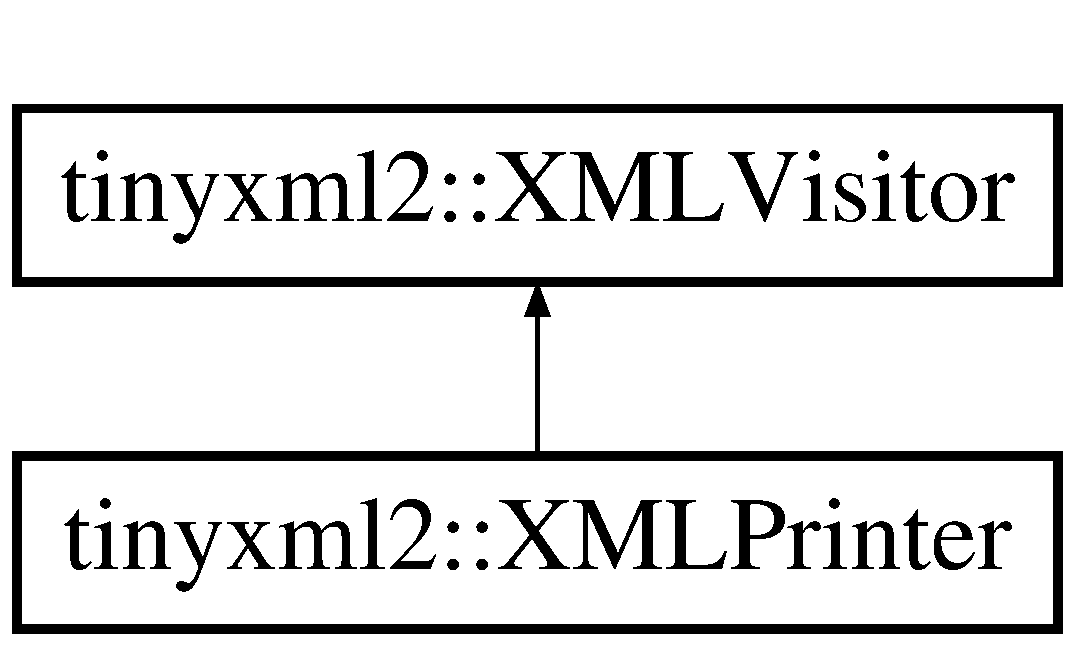
\includegraphics[height=2.000000cm]{classtinyxml2_1_1_x_m_l_visitor}
\end{center}
\end{figure}
\subsection*{Public Member Functions}
\begin{DoxyCompactItemize}
\item 
virtual \textbf{ $\sim$\+X\+M\+L\+Visitor} ()
\item 
virtual bool \textbf{ Visit\+Enter} (const \textbf{ X\+M\+L\+Document} \&)
\begin{DoxyCompactList}\small\item\em Visit a document. \end{DoxyCompactList}\item 
virtual bool \textbf{ Visit\+Exit} (const \textbf{ X\+M\+L\+Document} \&)
\begin{DoxyCompactList}\small\item\em Visit a document. \end{DoxyCompactList}\item 
virtual bool \textbf{ Visit\+Enter} (const \textbf{ X\+M\+L\+Element} \&, const \textbf{ X\+M\+L\+Attribute} $\ast$)
\begin{DoxyCompactList}\small\item\em Visit an element. \end{DoxyCompactList}\item 
virtual bool \textbf{ Visit\+Exit} (const \textbf{ X\+M\+L\+Element} \&)
\begin{DoxyCompactList}\small\item\em Visit an element. \end{DoxyCompactList}\item 
virtual bool \textbf{ Visit} (const \textbf{ X\+M\+L\+Declaration} \&)
\begin{DoxyCompactList}\small\item\em Visit a declaration. \end{DoxyCompactList}\item 
virtual bool \textbf{ Visit} (const \textbf{ X\+M\+L\+Text} \&)
\begin{DoxyCompactList}\small\item\em Visit a text node. \end{DoxyCompactList}\item 
virtual bool \textbf{ Visit} (const \textbf{ X\+M\+L\+Comment} \&)
\begin{DoxyCompactList}\small\item\em Visit a comment node. \end{DoxyCompactList}\item 
virtual bool \textbf{ Visit} (const \textbf{ X\+M\+L\+Unknown} \&)
\begin{DoxyCompactList}\small\item\em Visit an unknown node. \end{DoxyCompactList}\end{DoxyCompactItemize}


\subsection{Detailed Description}
Implements the interface to the \char`\"{}\+Visitor pattern\char`\"{} (see the Accept() method.) If you call the Accept() method, it requires being passed a \doxyref{X\+M\+L\+Visitor}{p.}{classtinyxml2_1_1_x_m_l_visitor} class to handle callbacks. For nodes that contain other nodes (Document, Element) you will get called with a Visit\+Enter/\+Visit\+Exit pair. Nodes that are always leafs are simply called with \doxyref{Visit()}{p.}{classtinyxml2_1_1_x_m_l_visitor_adc75bd459fc7ba8223b50f0616767f9a}.

If you return \textquotesingle{}true\textquotesingle{} from a Visit method, recursive parsing will continue. If you return false, {\bfseries{no children of this node or its siblings}} will be visited.

All flavors of Visit methods have a default implementation that returns \textquotesingle{}true\textquotesingle{} (continue visiting). You need to only override methods that are interesting to you.

Generally Accept() is called on the \doxyref{X\+M\+L\+Document}{p.}{classtinyxml2_1_1_x_m_l_document}, although all nodes support visiting.

You should never change the document from a callback.

\begin{DoxySeeAlso}{See also}
\doxyref{X\+M\+L\+Node\+::\+Accept()}{p.}{classtinyxml2_1_1_x_m_l_node_a81e66df0a44c67a7af17f3b77a152785} 
\end{DoxySeeAlso}


Definition at line 480 of file tinyxml2.\+h.



\subsection{Constructor \& Destructor Documentation}
\mbox{\label{classtinyxml2_1_1_x_m_l_visitor_a494e72033d646c47d9c65c502ec62364}} 
\index{tinyxml2::XMLVisitor@{tinyxml2::XMLVisitor}!````~XMLVisitor@{$\sim$XMLVisitor}}
\index{````~XMLVisitor@{$\sim$XMLVisitor}!tinyxml2::XMLVisitor@{tinyxml2::XMLVisitor}}
\subsubsection{$\sim$XMLVisitor()}
{\footnotesize\ttfamily virtual tinyxml2\+::\+X\+M\+L\+Visitor\+::$\sim$\+X\+M\+L\+Visitor (\begin{DoxyParamCaption}{ }\end{DoxyParamCaption})\hspace{0.3cm}{\ttfamily [inline]}, {\ttfamily [virtual]}}



Definition at line 483 of file tinyxml2.\+h.



\subsection{Member Function Documentation}
\mbox{\label{classtinyxml2_1_1_x_m_l_visitor_adc75bd459fc7ba8223b50f0616767f9a}} 
\index{tinyxml2::XMLVisitor@{tinyxml2::XMLVisitor}!Visit@{Visit}}
\index{Visit@{Visit}!tinyxml2::XMLVisitor@{tinyxml2::XMLVisitor}}
\subsubsection{Visit()\hspace{0.1cm}{\footnotesize\ttfamily [1/4]}}
{\footnotesize\ttfamily virtual bool tinyxml2\+::\+X\+M\+L\+Visitor\+::\+Visit (\begin{DoxyParamCaption}\item[{const \textbf{ X\+M\+L\+Declaration} \&}]{ }\end{DoxyParamCaption})\hspace{0.3cm}{\ttfamily [inline]}, {\ttfamily [virtual]}}



Visit a declaration. 



Reimplemented in \textbf{ tinyxml2\+::\+X\+M\+L\+Printer} \doxyref{}{p.}{classtinyxml2_1_1_x_m_l_printer_acfc625b2549304b9c7eb85ebd5c5eb39}.



Definition at line 504 of file tinyxml2.\+h.



Referenced by tinyxml2\+::\+X\+M\+L\+Text\+::\+Accept(), tinyxml2\+::\+X\+M\+L\+Comment\+::\+Accept(), tinyxml2\+::\+X\+M\+L\+Declaration\+::\+Accept(), and tinyxml2\+::\+X\+M\+L\+Unknown\+::\+Accept().

\mbox{\label{classtinyxml2_1_1_x_m_l_visitor_af30233565856480ea48b6fa0d6dec65b}} 
\index{tinyxml2::XMLVisitor@{tinyxml2::XMLVisitor}!Visit@{Visit}}
\index{Visit@{Visit}!tinyxml2::XMLVisitor@{tinyxml2::XMLVisitor}}
\subsubsection{Visit()\hspace{0.1cm}{\footnotesize\ttfamily [2/4]}}
{\footnotesize\ttfamily virtual bool tinyxml2\+::\+X\+M\+L\+Visitor\+::\+Visit (\begin{DoxyParamCaption}\item[{const \textbf{ X\+M\+L\+Text} \&}]{ }\end{DoxyParamCaption})\hspace{0.3cm}{\ttfamily [inline]}, {\ttfamily [virtual]}}



Visit a text node. 



Reimplemented in \textbf{ tinyxml2\+::\+X\+M\+L\+Printer} \doxyref{}{p.}{classtinyxml2_1_1_x_m_l_printer_adc0e42b4f6fcb90a95630c79575d030b}.



Definition at line 508 of file tinyxml2.\+h.

\mbox{\label{classtinyxml2_1_1_x_m_l_visitor_acc8147fb5a85f6c65721654e427752d7}} 
\index{tinyxml2::XMLVisitor@{tinyxml2::XMLVisitor}!Visit@{Visit}}
\index{Visit@{Visit}!tinyxml2::XMLVisitor@{tinyxml2::XMLVisitor}}
\subsubsection{Visit()\hspace{0.1cm}{\footnotesize\ttfamily [3/4]}}
{\footnotesize\ttfamily virtual bool tinyxml2\+::\+X\+M\+L\+Visitor\+::\+Visit (\begin{DoxyParamCaption}\item[{const \textbf{ X\+M\+L\+Comment} \&}]{ }\end{DoxyParamCaption})\hspace{0.3cm}{\ttfamily [inline]}, {\ttfamily [virtual]}}



Visit a comment node. 



Reimplemented in \textbf{ tinyxml2\+::\+X\+M\+L\+Printer} \doxyref{}{p.}{classtinyxml2_1_1_x_m_l_printer_aa294c5c01af0ebb9114902456e4cb53c}.



Definition at line 512 of file tinyxml2.\+h.

\mbox{\label{classtinyxml2_1_1_x_m_l_visitor_a14e4748387c34bf53d24e8119bb1f292}} 
\index{tinyxml2::XMLVisitor@{tinyxml2::XMLVisitor}!Visit@{Visit}}
\index{Visit@{Visit}!tinyxml2::XMLVisitor@{tinyxml2::XMLVisitor}}
\subsubsection{Visit()\hspace{0.1cm}{\footnotesize\ttfamily [4/4]}}
{\footnotesize\ttfamily virtual bool tinyxml2\+::\+X\+M\+L\+Visitor\+::\+Visit (\begin{DoxyParamCaption}\item[{const \textbf{ X\+M\+L\+Unknown} \&}]{ }\end{DoxyParamCaption})\hspace{0.3cm}{\ttfamily [inline]}, {\ttfamily [virtual]}}



Visit an unknown node. 



Reimplemented in \textbf{ tinyxml2\+::\+X\+M\+L\+Printer} \doxyref{}{p.}{classtinyxml2_1_1_x_m_l_printer_ab8af5455bbf9e4be2663e6642fcd7e32}.



Definition at line 516 of file tinyxml2.\+h.

\mbox{\label{classtinyxml2_1_1_x_m_l_visitor_acb3c22fc5f60eb9db98f533f2761f67d}} 
\index{tinyxml2::XMLVisitor@{tinyxml2::XMLVisitor}!VisitEnter@{VisitEnter}}
\index{VisitEnter@{VisitEnter}!tinyxml2::XMLVisitor@{tinyxml2::XMLVisitor}}
\subsubsection{VisitEnter()\hspace{0.1cm}{\footnotesize\ttfamily [1/2]}}
{\footnotesize\ttfamily virtual bool tinyxml2\+::\+X\+M\+L\+Visitor\+::\+Visit\+Enter (\begin{DoxyParamCaption}\item[{const \textbf{ X\+M\+L\+Document} \&}]{ }\end{DoxyParamCaption})\hspace{0.3cm}{\ttfamily [inline]}, {\ttfamily [virtual]}}



Visit a document. 



Reimplemented in \textbf{ tinyxml2\+::\+X\+M\+L\+Printer} \doxyref{}{p.}{classtinyxml2_1_1_x_m_l_printer_a9aa1de11a55a07db55a90fde37d7afad}.



Definition at line 486 of file tinyxml2.\+h.



Referenced by tinyxml2\+::\+X\+M\+L\+Element\+::\+Accept(), and tinyxml2\+::\+X\+M\+L\+Document\+::\+Accept().

\mbox{\label{classtinyxml2_1_1_x_m_l_visitor_af97980a17dd4e37448b181f5ddfa92b5}} 
\index{tinyxml2::XMLVisitor@{tinyxml2::XMLVisitor}!VisitEnter@{VisitEnter}}
\index{VisitEnter@{VisitEnter}!tinyxml2::XMLVisitor@{tinyxml2::XMLVisitor}}
\subsubsection{VisitEnter()\hspace{0.1cm}{\footnotesize\ttfamily [2/2]}}
{\footnotesize\ttfamily virtual bool tinyxml2\+::\+X\+M\+L\+Visitor\+::\+Visit\+Enter (\begin{DoxyParamCaption}\item[{const \textbf{ X\+M\+L\+Element} \&}]{,  }\item[{const \textbf{ X\+M\+L\+Attribute} $\ast$}]{ }\end{DoxyParamCaption})\hspace{0.3cm}{\ttfamily [inline]}, {\ttfamily [virtual]}}



Visit an element. 



Reimplemented in \textbf{ tinyxml2\+::\+X\+M\+L\+Printer} \doxyref{}{p.}{classtinyxml2_1_1_x_m_l_printer_a169b2509d8eabb70811b2bb8cfd1f5d1}.



Definition at line 495 of file tinyxml2.\+h.

\mbox{\label{classtinyxml2_1_1_x_m_l_visitor_a170e9989cd046ba904f302d087e07086}} 
\index{tinyxml2::XMLVisitor@{tinyxml2::XMLVisitor}!VisitExit@{VisitExit}}
\index{VisitExit@{VisitExit}!tinyxml2::XMLVisitor@{tinyxml2::XMLVisitor}}
\subsubsection{VisitExit()\hspace{0.1cm}{\footnotesize\ttfamily [1/2]}}
{\footnotesize\ttfamily virtual bool tinyxml2\+::\+X\+M\+L\+Visitor\+::\+Visit\+Exit (\begin{DoxyParamCaption}\item[{const \textbf{ X\+M\+L\+Document} \&}]{ }\end{DoxyParamCaption})\hspace{0.3cm}{\ttfamily [inline]}, {\ttfamily [virtual]}}



Visit a document. 



Reimplemented in \textbf{ tinyxml2\+::\+X\+M\+L\+Printer} \doxyref{}{p.}{classtinyxml2_1_1_x_m_l_printer_a15fc1f2b922f540917dcf52808737b29}.



Definition at line 490 of file tinyxml2.\+h.



Referenced by tinyxml2\+::\+X\+M\+L\+Element\+::\+Accept(), and tinyxml2\+::\+X\+M\+L\+Document\+::\+Accept().

\mbox{\label{classtinyxml2_1_1_x_m_l_visitor_a772f10ddc83f881956d32628faa16eb6}} 
\index{tinyxml2::XMLVisitor@{tinyxml2::XMLVisitor}!VisitExit@{VisitExit}}
\index{VisitExit@{VisitExit}!tinyxml2::XMLVisitor@{tinyxml2::XMLVisitor}}
\subsubsection{VisitExit()\hspace{0.1cm}{\footnotesize\ttfamily [2/2]}}
{\footnotesize\ttfamily virtual bool tinyxml2\+::\+X\+M\+L\+Visitor\+::\+Visit\+Exit (\begin{DoxyParamCaption}\item[{const \textbf{ X\+M\+L\+Element} \&}]{ }\end{DoxyParamCaption})\hspace{0.3cm}{\ttfamily [inline]}, {\ttfamily [virtual]}}



Visit an element. 



Reimplemented in \textbf{ tinyxml2\+::\+X\+M\+L\+Printer} \doxyref{}{p.}{classtinyxml2_1_1_x_m_l_printer_a2edd48405971a88951c71c9df86a2f50}.



Definition at line 499 of file tinyxml2.\+h.



The documentation for this class was generated from the following file\+:\begin{DoxyCompactItemize}
\item 
include/\textbf{ tinyxml2.\+h}\end{DoxyCompactItemize}

\chapter{File Documentation}
\hypertarget{_agent_8h}{}\section{include/\+Agent.h File Reference}
\label{_agent_8h}\index{include/Agent.h@{include/Agent.h}}
{\ttfamily \#include $<$Map.\+h$>$}\newline
{\ttfamily \#include $<$Clock.\+h$>$}\newline
{\ttfamily \#include $<$string$>$}\newline
Include dependency graph for Agent.\+h\+:\nopagebreak
\begin{figure}[H]
\begin{center}
\leavevmode
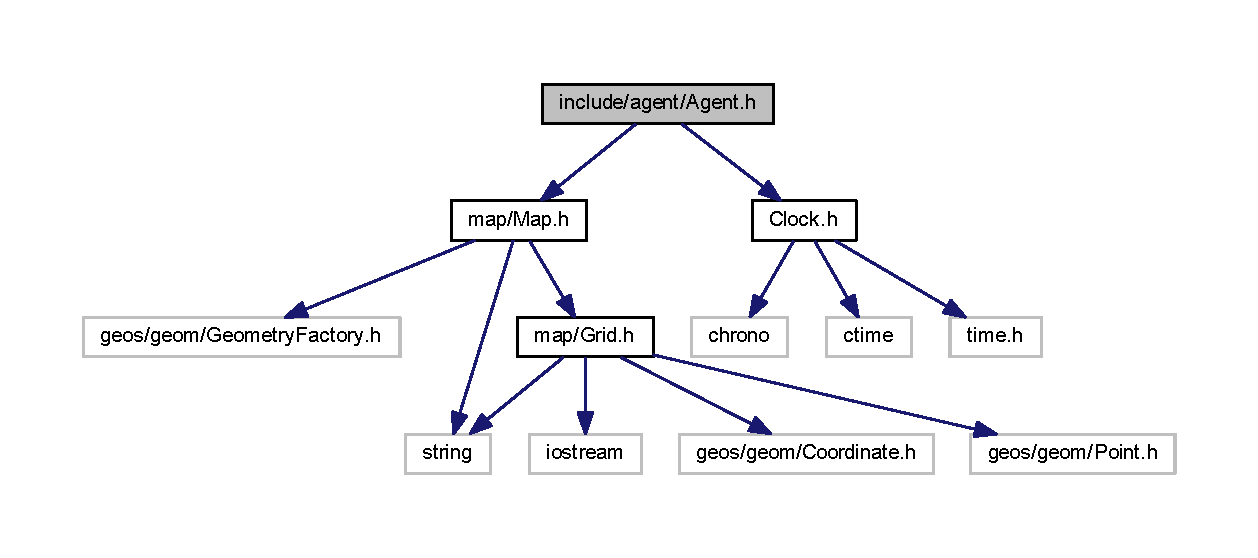
\includegraphics[width=350pt]{_agent_8h__incl}
\end{center}
\end{figure}
This graph shows which files directly or indirectly include this file\+:\nopagebreak
\begin{figure}[H]
\begin{center}
\leavevmode
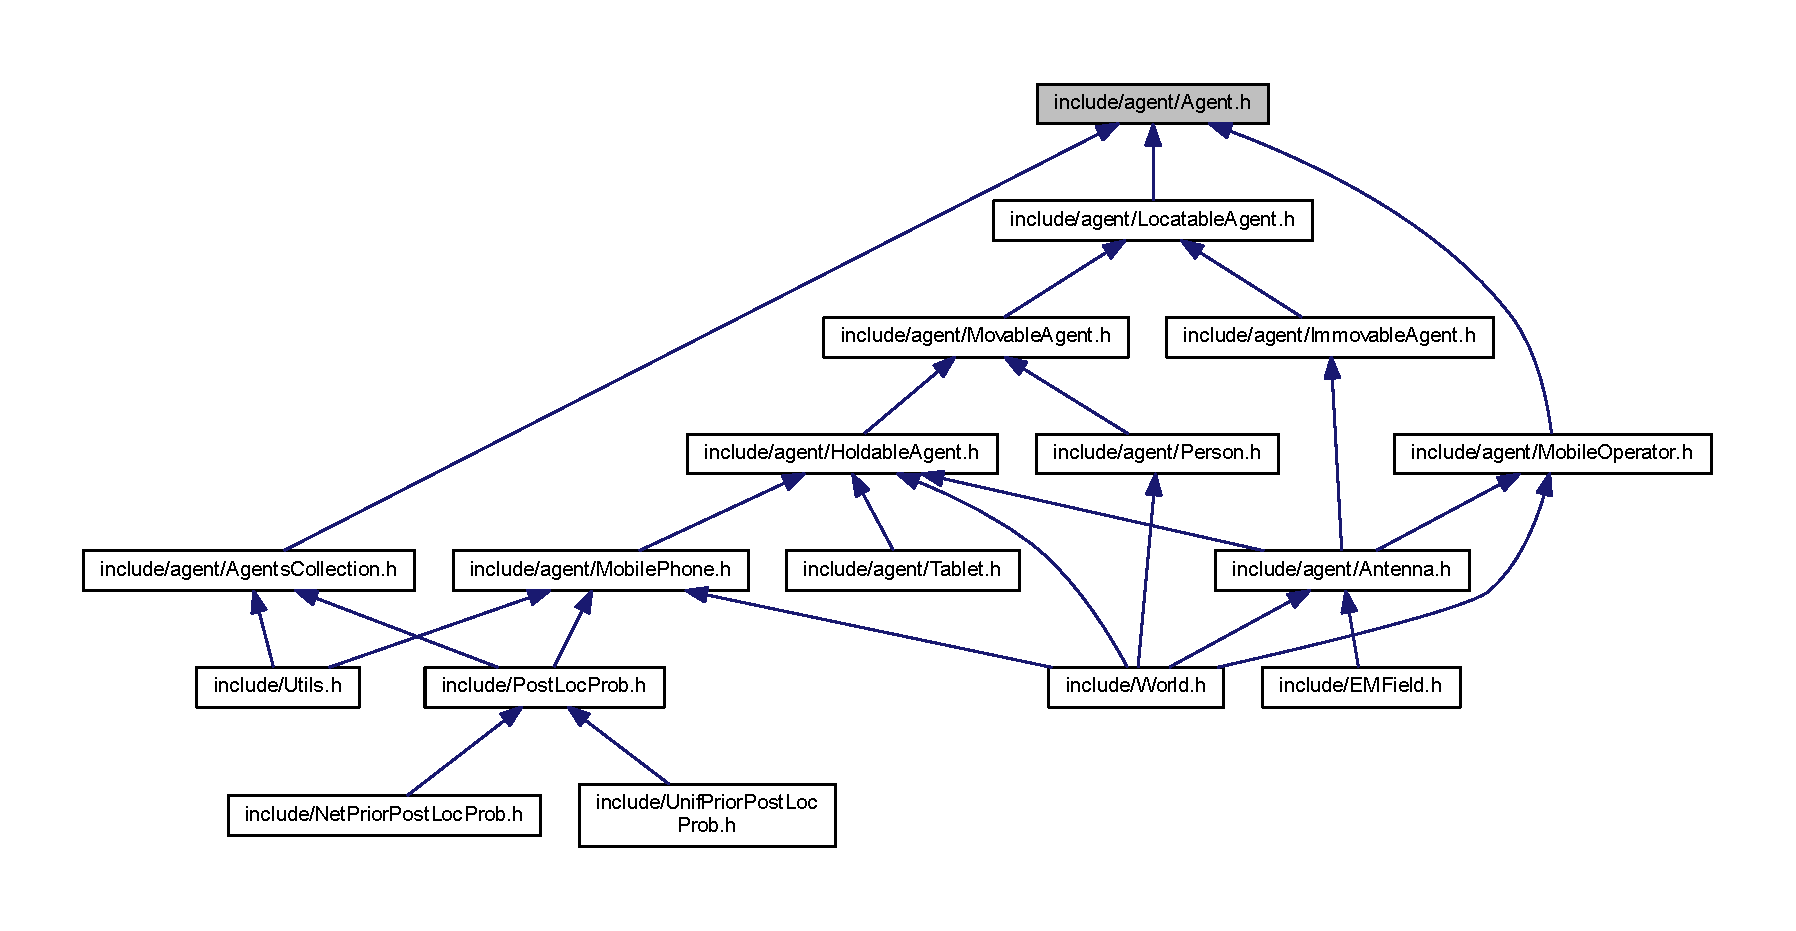
\includegraphics[width=350pt]{_agent_8h__dep__incl}
\end{center}
\end{figure}
\subsection*{Classes}
\begin{DoxyCompactItemize}
\item 
class \mbox{\hyperlink{class_agent}{Agent}}
\end{DoxyCompactItemize}

\hypertarget{_agents_collection_8h}{}\section{include/\+Agents\+Collection.h File Reference}
\label{_agents_collection_8h}\index{include/AgentsCollection.h@{include/AgentsCollection.h}}
{\ttfamily \#include $<$Agent.\+h$>$}\newline
{\ttfamily \#include $<$typeinfo$>$}\newline
{\ttfamily \#include $<$unordered\+\_\+map$>$}\newline
{\ttfamily \#include $<$vector$>$}\newline
Include dependency graph for Agents\+Collection.\+h\+:\nopagebreak
\begin{figure}[H]
\begin{center}
\leavevmode
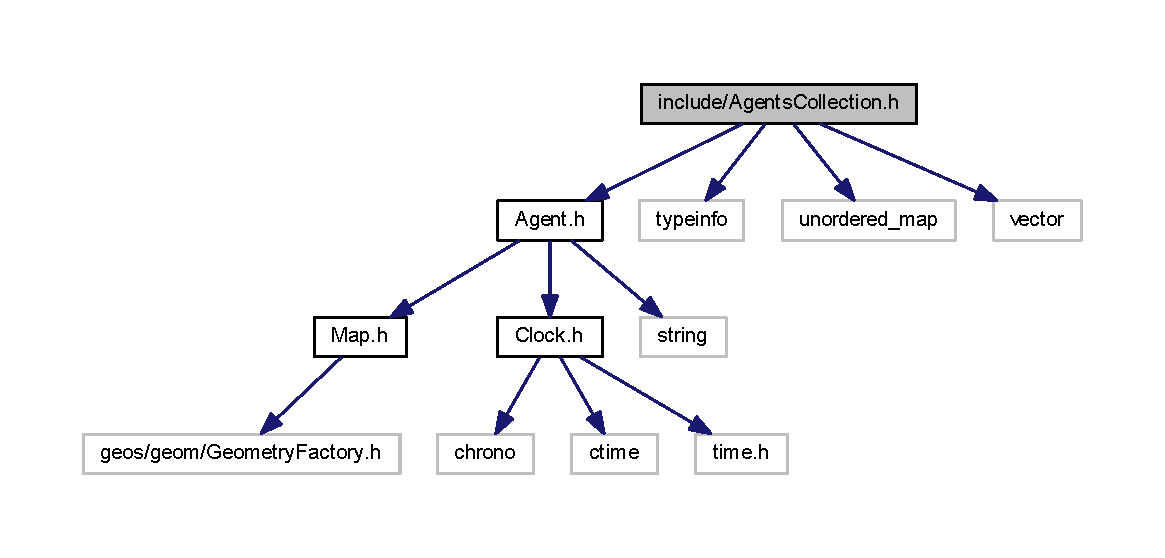
\includegraphics[width=350pt]{_agents_collection_8h__incl}
\end{center}
\end{figure}
This graph shows which files directly or indirectly include this file\+:\nopagebreak
\begin{figure}[H]
\begin{center}
\leavevmode
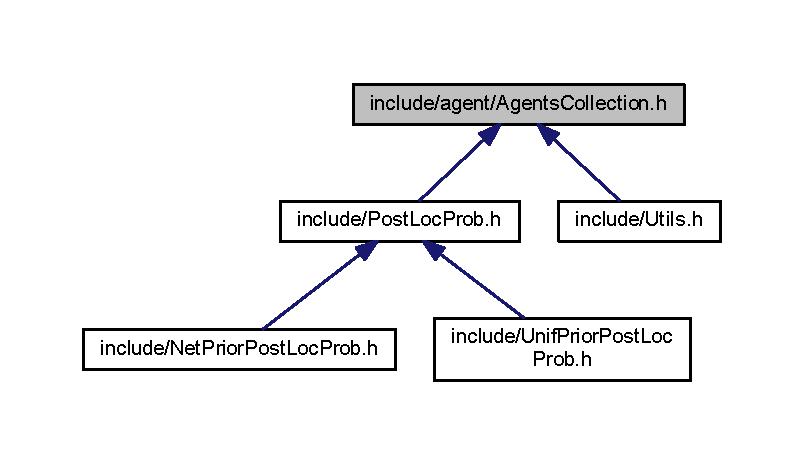
\includegraphics[width=269pt]{_agents_collection_8h__dep__incl}
\end{center}
\end{figure}
\subsection*{Classes}
\begin{DoxyCompactItemize}
\item 
class \mbox{\hyperlink{class_agents_collection}{Agents\+Collection}}
\end{DoxyCompactItemize}
\subsection*{Typedefs}
\begin{DoxyCompactItemize}
\item 
typedef unordered\+\_\+multimap$<$ string, \mbox{\hyperlink{class_agent}{Agent}} $\ast$ $>$\+::iterator \mbox{\hyperlink{_agents_collection_8h_afde47bc45d604b8b8c72755072376679}{um\+\_\+iterator}}
\end{DoxyCompactItemize}


\subsection{Typedef Documentation}
\mbox{\Hypertarget{_agents_collection_8h_afde47bc45d604b8b8c72755072376679}\label{_agents_collection_8h_afde47bc45d604b8b8c72755072376679}} 
\index{AgentsCollection.h@{AgentsCollection.h}!um\_iterator@{um\_iterator}}
\index{um\_iterator@{um\_iterator}!AgentsCollection.h@{AgentsCollection.h}}
\subsubsection{\texorpdfstring{um\_iterator}{um\_iterator}}
{\footnotesize\ttfamily typedef unordered\+\_\+multimap$<$string, \mbox{\hyperlink{class_agent}{Agent}}$\ast$$>$\+::iterator \mbox{\hyperlink{_agents_collection_8h_afde47bc45d604b8b8c72755072376679}{um\+\_\+iterator}}}


\section{include/\+Antenna.h File Reference}
\label{_antenna_8h}\index{include/\+Antenna.\+h@{include/\+Antenna.\+h}}
{\ttfamily \#include $<$Immovable\+Agent.\+h$>$}\newline
{\ttfamily \#include $<$Holdable\+Agent.\+h$>$}\newline
{\ttfamily \#include $<$geos/geom/\+Polygon.\+h$>$}\newline
{\ttfamily \#include $<$Event\+Type.\+h$>$}\newline
{\ttfamily \#include $<$Antenna\+Type.\+h$>$}\newline
{\ttfamily \#include $<$string$>$}\newline
{\ttfamily \#include $<$fstream$>$}\newline
{\ttfamily \#include $<$tinyxml2.\+h$>$}\newline
Include dependency graph for Antenna.\+h\+:
% FIG 0
This graph shows which files directly or indirectly include this file\+:
% FIG 1
\subsection*{Classes}
\begin{DoxyCompactItemize}
\item 
class \textbf{ Antenna}
\end{DoxyCompactItemize}

\hypertarget{_antenna_info_8h}{}\section{include/\+Antenna\+Info.h File Reference}
\label{_antenna_info_8h}\index{include/AntennaInfo.h@{include/AntennaInfo.h}}
{\ttfamily \#include $<$string$>$}\newline
Include dependency graph for Antenna\+Info.\+h\+:
\nopagebreak
\begin{figure}[H]
\begin{center}
\leavevmode
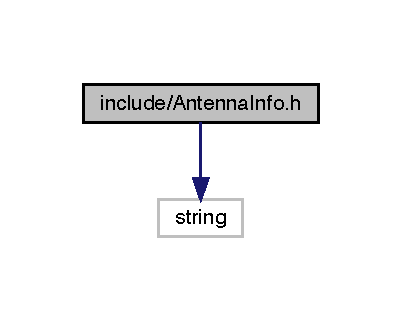
\includegraphics[width=193pt]{_antenna_info_8h__incl}
\end{center}
\end{figure}
This graph shows which files directly or indirectly include this file\+:
\nopagebreak
\begin{figure}[H]
\begin{center}
\leavevmode
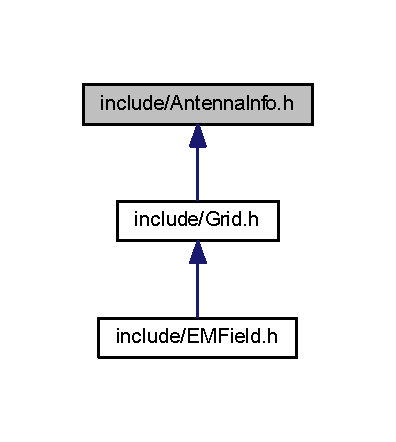
\includegraphics[width=193pt]{_antenna_info_8h__dep__incl}
\end{center}
\end{figure}
\subsection*{Classes}
\begin{DoxyCompactItemize}
\item 
class \mbox{\hyperlink{class_antenna_info}{Antenna\+Info}}
\end{DoxyCompactItemize}

\section{include/\+Antenna\+Type.h File Reference}
\label{_antenna_type_8h}\index{include/AntennaType.h@{include/AntennaType.h}}
\subsection*{Enumerations}
\begin{DoxyCompactItemize}
\item 
enum \textbf{ Antenna\+Type} \{ \textbf{ Antenna\+Type\+::\+O\+M\+N\+I\+D\+I\+R\+E\+C\+T\+I\+O\+N\+AL}, 
\textbf{ Antenna\+Type\+::\+D\+I\+R\+E\+C\+T\+I\+O\+N\+AL}
 \}
\end{DoxyCompactItemize}


\subsection{Enumeration Type Documentation}
\mbox{\label{_antenna_type_8h_a7b678b5cb9dedc607131200119d96b16}} 
\index{AntennaType.h@{AntennaType.h}!AntennaType@{AntennaType}}
\index{AntennaType@{AntennaType}!AntennaType.h@{AntennaType.h}}
\subsubsection{AntennaType}
{\footnotesize\ttfamily enum \textbf{ Antenna\+Type}\hspace{0.3cm}{\ttfamily [strong]}}

An enum class that is used to represent the type of an antenna. \begin{DoxyEnumFields}{Enumerator}
\raisebox{\heightof{T}}[0pt][0pt]{\index{OMNIDIRECTIONAL@{OMNIDIRECTIONAL}!AntennaType.h@{AntennaType.h}}\index{AntennaType.h@{AntennaType.h}!OMNIDIRECTIONAL@{OMNIDIRECTIONAL}}}\mbox{\label{_antenna_type_8h_a7b678b5cb9dedc607131200119d96b16a8ff57fa72952e98025e600a041b8b8de}} 
O\+M\+N\+I\+D\+I\+R\+E\+C\+T\+I\+O\+N\+AL&\\
\hline

\raisebox{\heightof{T}}[0pt][0pt]{\index{DIRECTIONAL@{DIRECTIONAL}!AntennaType.h@{AntennaType.h}}\index{AntennaType.h@{AntennaType.h}!DIRECTIONAL@{DIRECTIONAL}}}\mbox{\label{_antenna_type_8h_a7b678b5cb9dedc607131200119d96b16ab6f2249394a4def60a78b342dcc925b9}} 
D\+I\+R\+E\+C\+T\+I\+O\+N\+AL&\\
\hline

\end{DoxyEnumFields}


Definition at line 16 of file Antenna\+Type.\+h.


\hypertarget{_clock_8h}{}\section{include/\+Clock.h File Reference}
\label{_clock_8h}\index{include/Clock.h@{include/Clock.h}}
{\ttfamily \#include $<$chrono$>$}\newline
{\ttfamily \#include $<$ctime$>$}\newline
{\ttfamily \#include $<$time.\+h$>$}\newline
Include dependency graph for Clock.\+h\+:\nopagebreak
\begin{figure}[H]
\begin{center}
\leavevmode
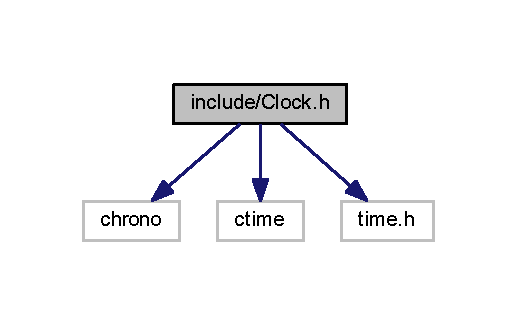
\includegraphics[width=246pt]{_clock_8h__incl}
\end{center}
\end{figure}
This graph shows which files directly or indirectly include this file\+:
\nopagebreak
\begin{figure}[H]
\begin{center}
\leavevmode
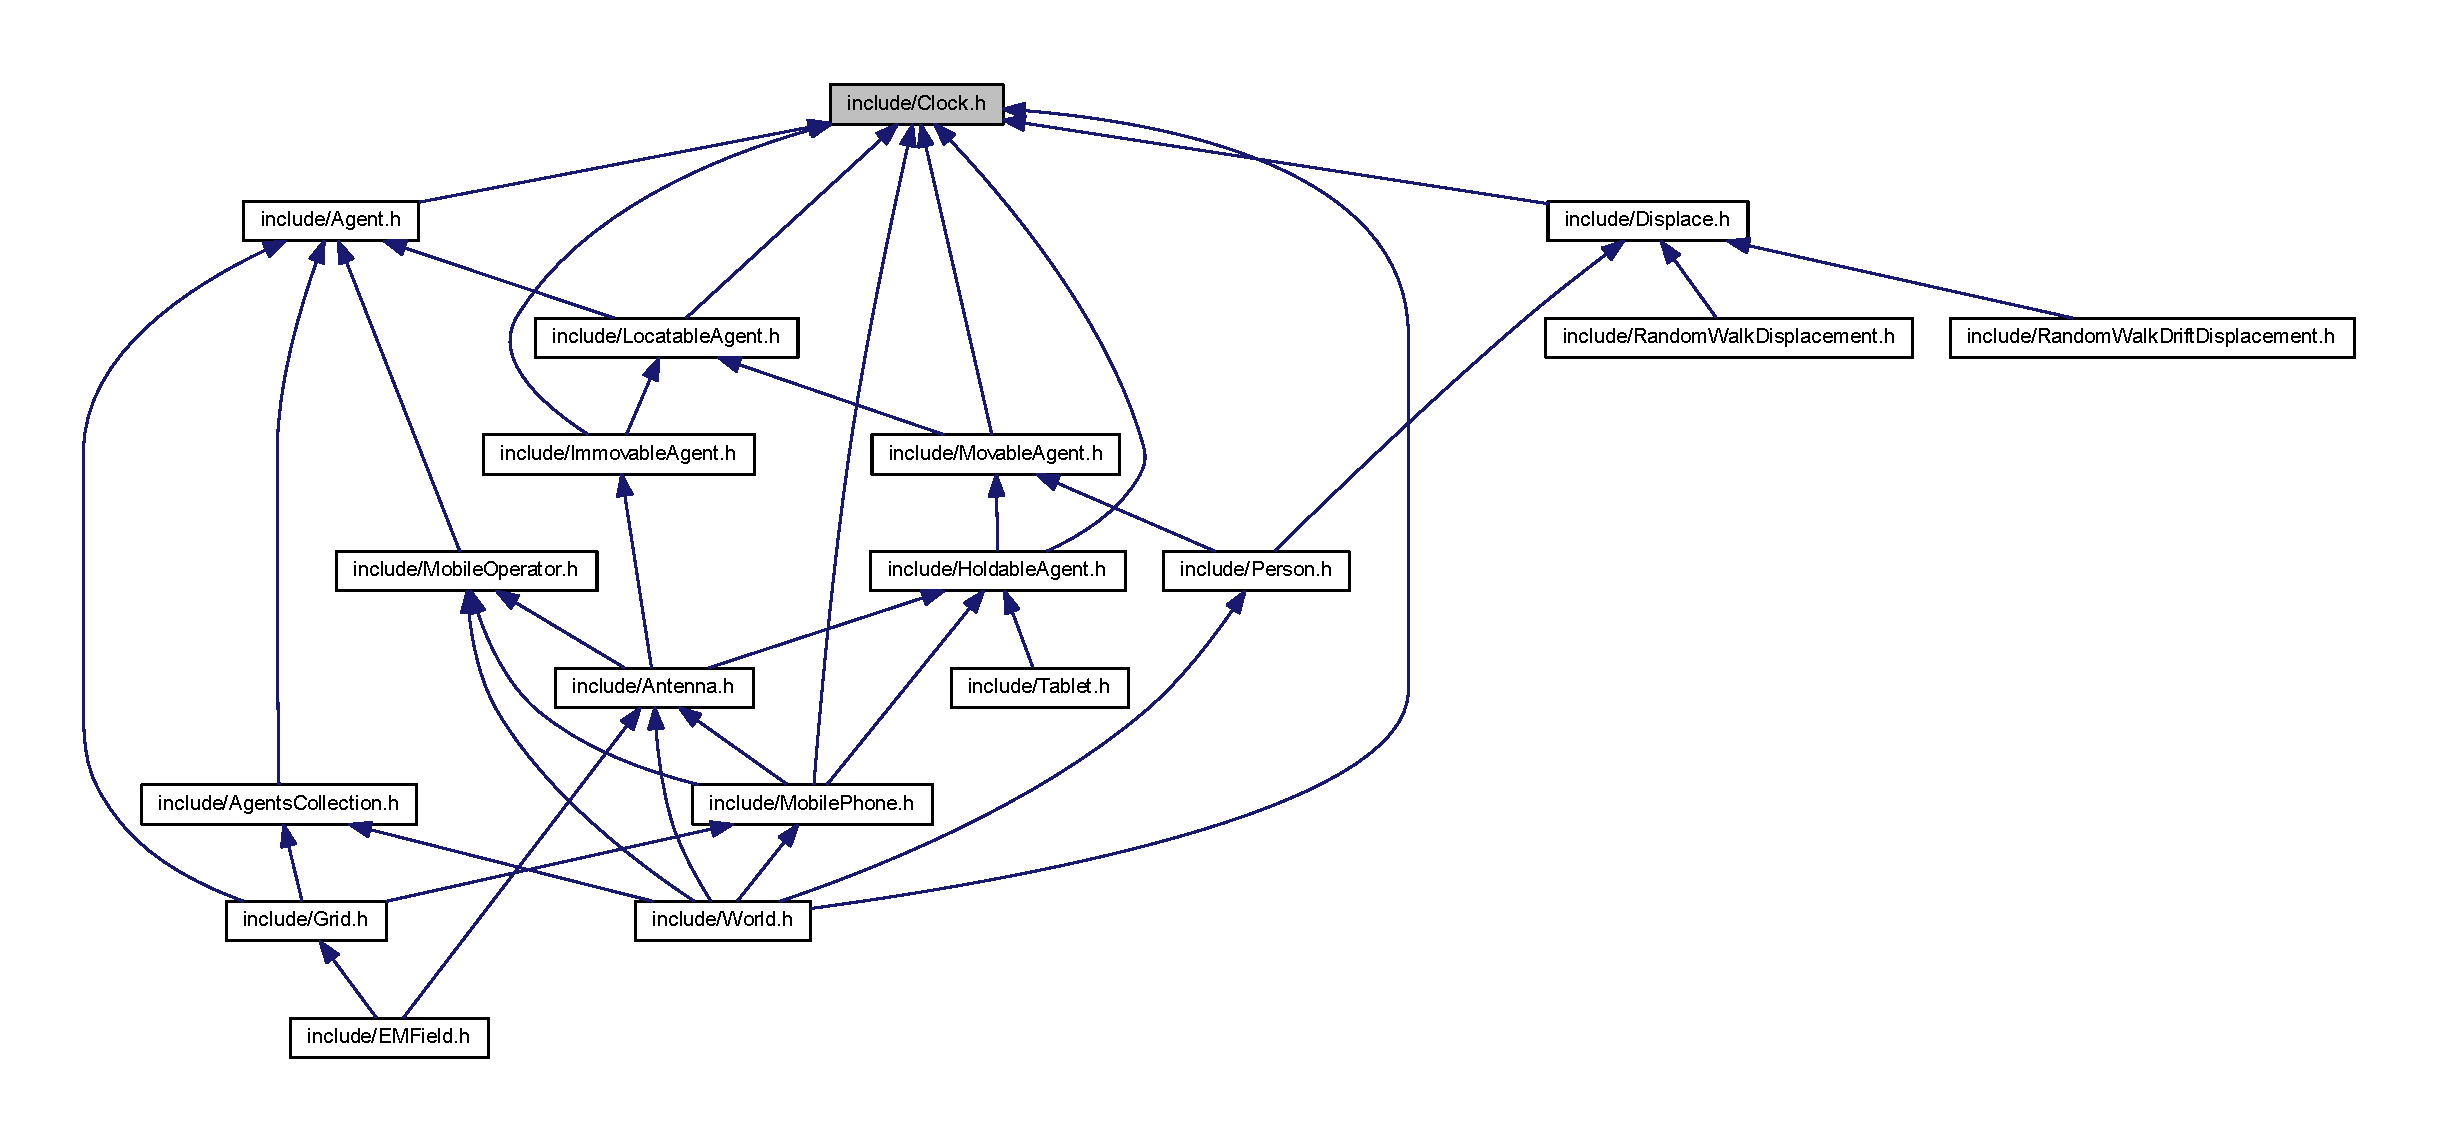
\includegraphics[width=350pt]{_clock_8h__dep__incl}
\end{center}
\end{figure}
\subsection*{Classes}
\begin{DoxyCompactItemize}
\item 
class \mbox{\hyperlink{class_clock}{Clock}}
\end{DoxyCompactItemize}

\section{include/\+Constants.h File Reference}
\label{_constants_8h}\index{include/Constants.h@{include/Constants.h}}
\subsection*{Classes}
\begin{DoxyCompactItemize}
\item 
class \textbf{ Constants}
\end{DoxyCompactItemize}

\section{include/\+C\+S\+Vparser.hpp File Reference}
\label{_c_s_vparser_8hpp}\index{include/CSVparser.hpp@{include/CSVparser.hpp}}
{\ttfamily \#include $<$stdexcept$>$}\newline
{\ttfamily \#include $<$string$>$}\newline
{\ttfamily \#include $<$vector$>$}\newline
{\ttfamily \#include $<$list$>$}\newline
{\ttfamily \#include $<$sstream$>$}\newline
\subsection*{Classes}
\begin{DoxyCompactItemize}
\item 
class \textbf{ Error}
\item 
class \textbf{ Row}
\item 
class \textbf{ Parser}
\end{DoxyCompactItemize}
\subsection*{Enumerations}
\begin{DoxyCompactItemize}
\item 
enum \textbf{ Data\+Type} \{ \textbf{ e\+F\+I\+LE} = 0, 
\textbf{ e\+P\+U\+RE} = 1
 \}
\end{DoxyCompactItemize}


\subsection{Enumeration Type Documentation}
\mbox{\label{_c_s_vparser_8hpp_ad8ed01ff3ff33333d8e19db4d2818bb6}} 
\index{CSVparser.hpp@{CSVparser.hpp}!DataType@{DataType}}
\index{DataType@{DataType}!CSVparser.hpp@{CSVparser.hpp}}
\subsubsection{DataType}
{\footnotesize\ttfamily enum \textbf{ Data\+Type}}

\begin{DoxyEnumFields}{Enumerator}
\raisebox{\heightof{T}}[0pt][0pt]{\index{eFILE@{eFILE}!CSVparser.hpp@{CSVparser.hpp}}\index{CSVparser.hpp@{CSVparser.hpp}!eFILE@{eFILE}}}\mbox{\label{_c_s_vparser_8hpp_ad8ed01ff3ff33333d8e19db4d2818bb6a99e2aefa5a03705fd10b8b72e081349f}} 
e\+F\+I\+LE&\\
\hline

\raisebox{\heightof{T}}[0pt][0pt]{\index{ePURE@{ePURE}!CSVparser.hpp@{CSVparser.hpp}}\index{CSVparser.hpp@{CSVparser.hpp}!ePURE@{ePURE}}}\mbox{\label{_c_s_vparser_8hpp_ad8ed01ff3ff33333d8e19db4d2818bb6aef7f347978c58a657566792291ec1e4b}} 
e\+P\+U\+RE&\\
\hline

\end{DoxyEnumFields}


Definition at line 53 of file C\+S\+Vparser.\+hpp.


\hypertarget{_e_m_field_8h}{}\section{include/\+E\+M\+Field.h File Reference}
\label{_e_m_field_8h}\index{include/EMField.h@{include/EMField.h}}
{\ttfamily \#include $<$Antenna.\+h$>$}\newline
{\ttfamily \#include $<$Constants.\+h$>$}\newline
{\ttfamily \#include $<$Grid.\+h$>$}\newline
{\ttfamily \#include $<$utility$>$}\newline
{\ttfamily \#include $<$vector$>$}\newline
{\ttfamily \#include $<$map$>$}\newline
Include dependency graph for E\+M\+Field.\+h\+:\nopagebreak
\begin{figure}[H]
\begin{center}
\leavevmode
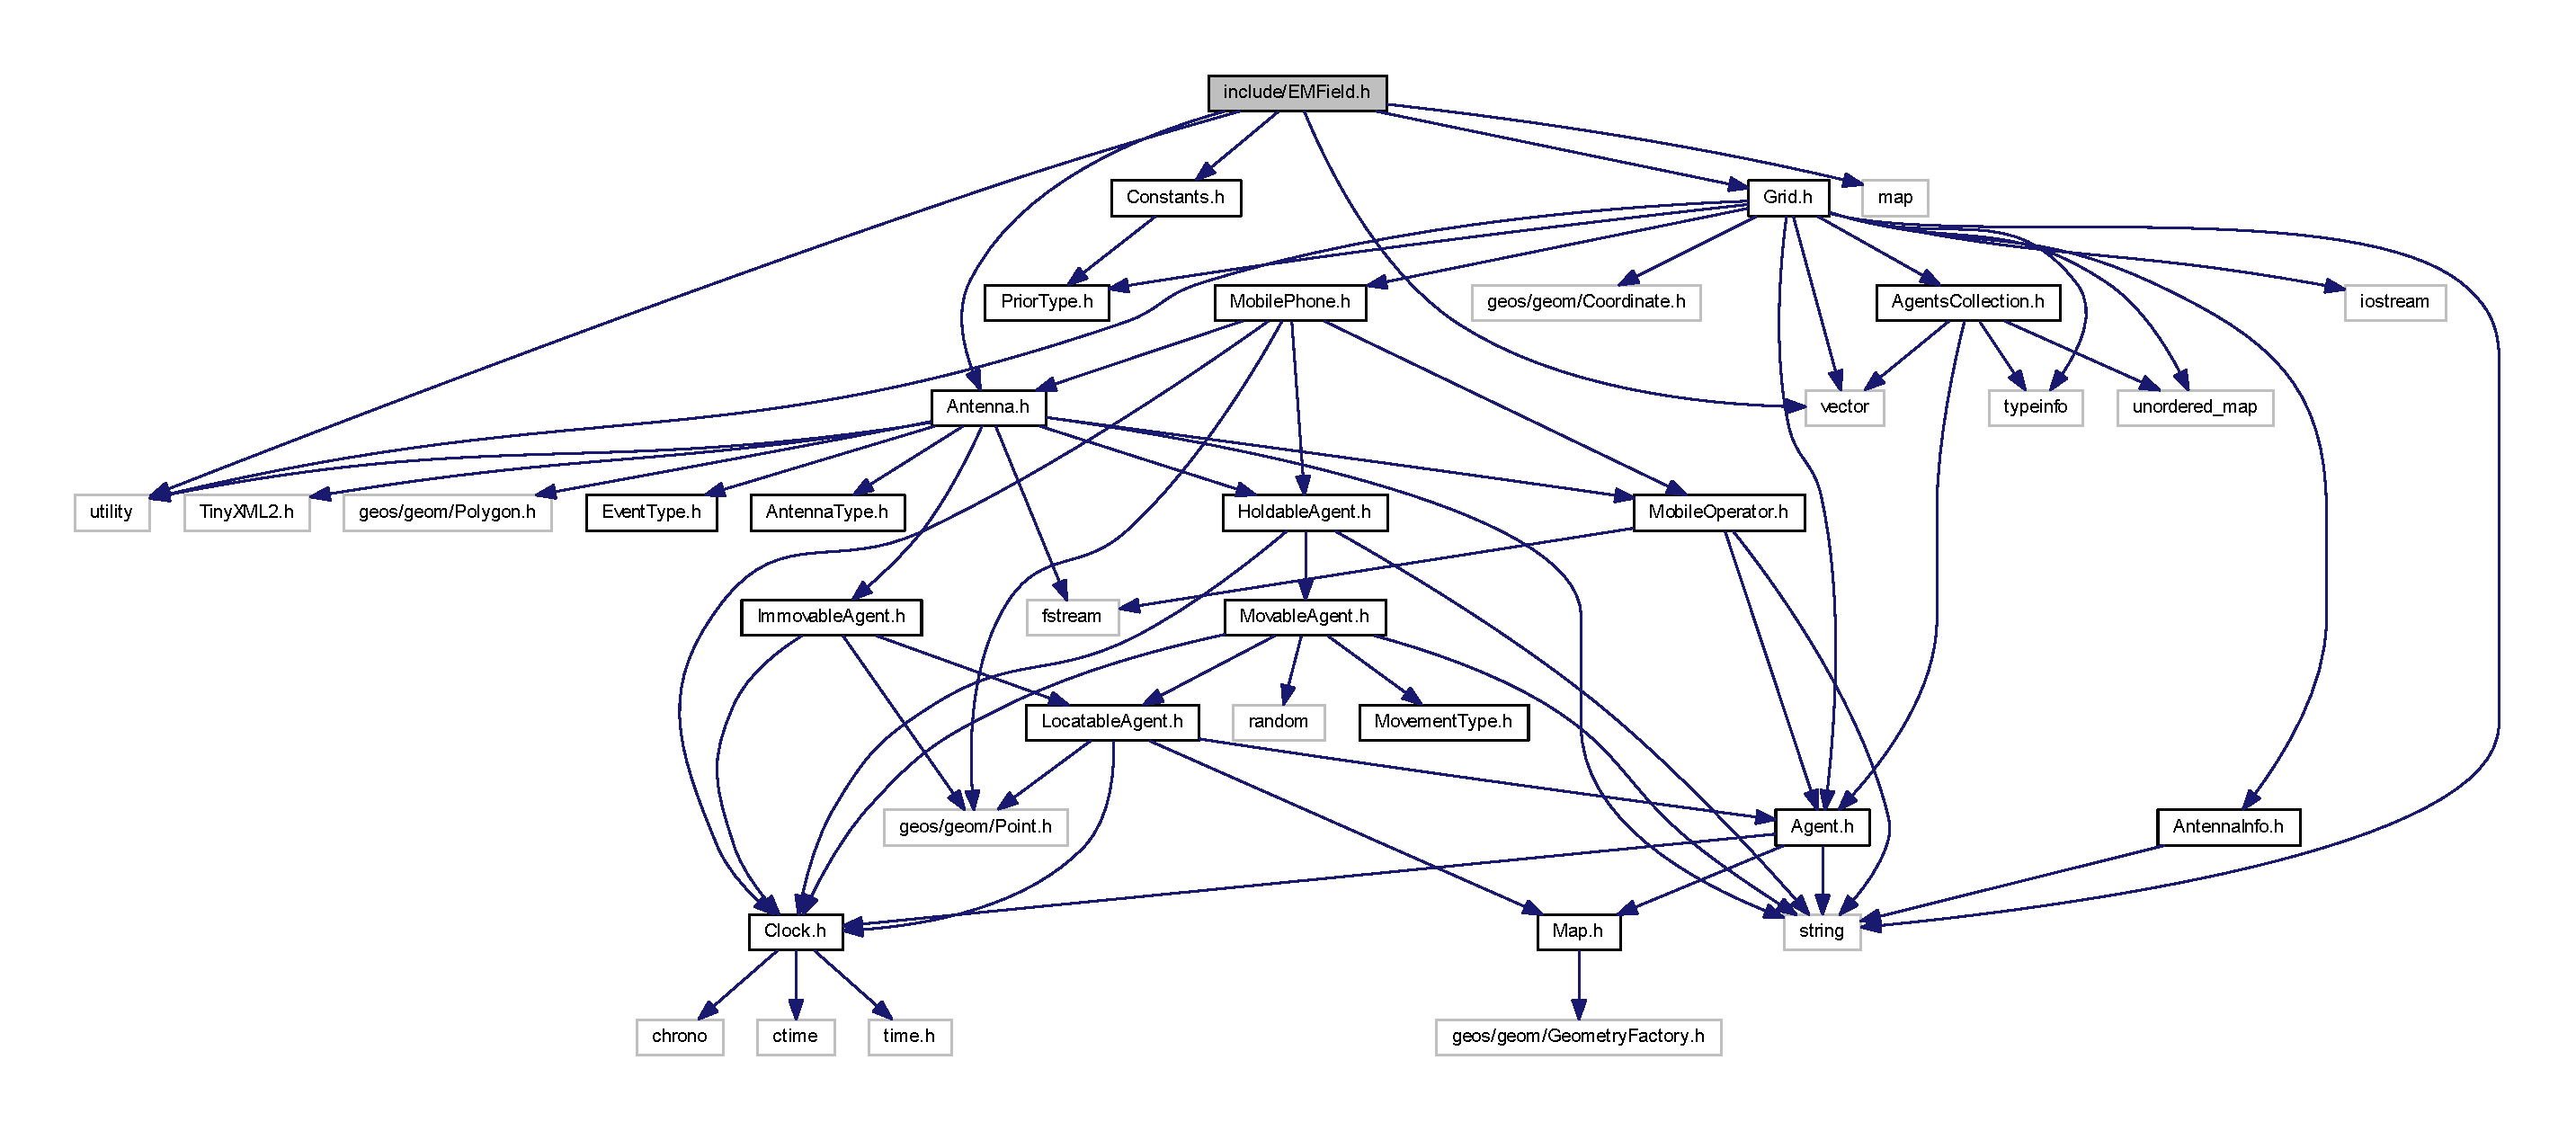
\includegraphics[width=350pt]{_e_m_field_8h__incl}
\end{center}
\end{figure}
\subsection*{Classes}
\begin{DoxyCompactItemize}
\item 
class \mbox{\hyperlink{class_e_m_field}{E\+M\+Field}}
\end{DoxyCompactItemize}

\hypertarget{_event_type_8h}{}\section{include/\+Event\+Type.h File Reference}
\label{_event_type_8h}\index{include/\+Event\+Type.\+h@{include/\+Event\+Type.\+h}}
This graph shows which files directly or indirectly include this file\+:\nopagebreak
\begin{figure}[H]
\begin{center}
\leavevmode
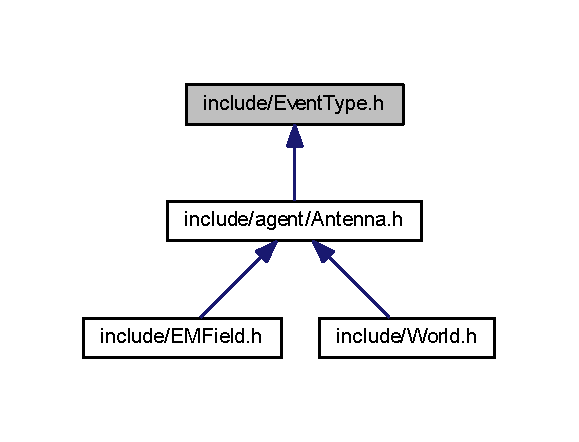
\includegraphics[width=306pt]{_event_type_8h__dep__incl}
\end{center}
\end{figure}
\subsection*{Enumerations}
\begin{DoxyCompactItemize}
\item 
enum \hyperlink{_event_type_8h_a2628ea8d12e8b2563c32f05dc7fff6fa}{Event\+Type} \{ \hyperlink{_event_type_8h_a2628ea8d12e8b2563c32f05dc7fff6faa9893a3a649e7100d87b1560bd8202ec2}{Event\+Type\+::\+A\+T\+T\+A\+C\+H\+\_\+\+D\+E\+V\+I\+CE}, 
\hyperlink{_event_type_8h_a2628ea8d12e8b2563c32f05dc7fff6faad4d5a45ac3a7a538879a9525fed18ddf}{Event\+Type\+::\+D\+E\+T\+A\+C\+H\+\_\+\+D\+E\+V\+I\+CE}, 
\hyperlink{_event_type_8h_a2628ea8d12e8b2563c32f05dc7fff6faaea76d50440d9cdc0ad1cac6ab9ac4f27}{Event\+Type\+::\+A\+L\+R\+E\+A\+D\+Y\+\_\+\+A\+T\+T\+A\+C\+H\+E\+D\+\_\+\+D\+E\+V\+I\+CE}, 
\hyperlink{_event_type_8h_a2628ea8d12e8b2563c32f05dc7fff6faa6ac0995df1d7ce888368dccf7af3e737}{Event\+Type\+::\+I\+N\+\_\+\+R\+A\+N\+G\+E\+\_\+\+N\+O\+T\+\_\+\+A\+T\+T\+A\+C\+H\+E\+D\+\_\+\+D\+E\+V\+I\+CE}
 \}
\end{DoxyCompactItemize}


\subsection{Enumeration Type Documentation}
\mbox{\Hypertarget{_event_type_8h_a2628ea8d12e8b2563c32f05dc7fff6fa}\label{_event_type_8h_a2628ea8d12e8b2563c32f05dc7fff6fa}} 
\index{Event\+Type.\+h@{Event\+Type.\+h}!Event\+Type@{Event\+Type}}
\index{Event\+Type@{Event\+Type}!Event\+Type.\+h@{Event\+Type.\+h}}
\subsubsection{\texorpdfstring{Event\+Type}{EventType}}
{\footnotesize\ttfamily enum \hyperlink{_event_type_8h_a2628ea8d12e8b2563c32f05dc7fff6fa}{Event\+Type}\hspace{0.3cm}{\ttfamily [strong]}}

This class is an enumeration of network events currently registered\+: A\+T\+T\+A\+C\+H\+\_\+\+D\+E\+V\+I\+CE -\/ means that an antenna connects a new mobile device. D\+E\+T\+A\+C\+H\+\_\+\+D\+E\+V\+I\+CE -\/ means that an antenna disconnects a mobile device, i.\+e. this mobile device is no longer connected to that antenna. A\+L\+R\+E\+A\+D\+Y\+\_\+\+A\+T\+T\+A\+C\+H\+E\+D\+\_\+\+D\+E\+V\+I\+CE -\/ means that an antenna is connected with a mobile device and that mobile was connected to the same antenna in the previous time step too. I\+N\+\_\+\+R\+A\+N\+G\+E\+\_\+\+N\+O\+T\+\_\+\+A\+T\+T\+A\+C\+H\+E\+D\+\_\+\+D\+E\+V\+I\+CE -\/ means that a mobile device tried to connect to an antenna, the antenna provided enough signal power/quality but the connection was not successful (for example antenna is at its maximum capacity and cannot connect any new devices). \begin{DoxyEnumFields}{Enumerator}
\raisebox{\heightof{T}}[0pt][0pt]{\index{A\+T\+T\+A\+C\+H\+\_\+\+D\+E\+V\+I\+CE@{A\+T\+T\+A\+C\+H\+\_\+\+D\+E\+V\+I\+CE}!Event\+Type.\+h@{Event\+Type.\+h}}\index{Event\+Type.\+h@{Event\+Type.\+h}!A\+T\+T\+A\+C\+H\+\_\+\+D\+E\+V\+I\+CE@{A\+T\+T\+A\+C\+H\+\_\+\+D\+E\+V\+I\+CE}}}\mbox{\Hypertarget{_event_type_8h_a2628ea8d12e8b2563c32f05dc7fff6faa9893a3a649e7100d87b1560bd8202ec2}\label{_event_type_8h_a2628ea8d12e8b2563c32f05dc7fff6faa9893a3a649e7100d87b1560bd8202ec2}} 
A\+T\+T\+A\+C\+H\+\_\+\+D\+E\+V\+I\+CE&\\
\hline

\raisebox{\heightof{T}}[0pt][0pt]{\index{D\+E\+T\+A\+C\+H\+\_\+\+D\+E\+V\+I\+CE@{D\+E\+T\+A\+C\+H\+\_\+\+D\+E\+V\+I\+CE}!Event\+Type.\+h@{Event\+Type.\+h}}\index{Event\+Type.\+h@{Event\+Type.\+h}!D\+E\+T\+A\+C\+H\+\_\+\+D\+E\+V\+I\+CE@{D\+E\+T\+A\+C\+H\+\_\+\+D\+E\+V\+I\+CE}}}\mbox{\Hypertarget{_event_type_8h_a2628ea8d12e8b2563c32f05dc7fff6faad4d5a45ac3a7a538879a9525fed18ddf}\label{_event_type_8h_a2628ea8d12e8b2563c32f05dc7fff6faad4d5a45ac3a7a538879a9525fed18ddf}} 
D\+E\+T\+A\+C\+H\+\_\+\+D\+E\+V\+I\+CE&\\
\hline

\raisebox{\heightof{T}}[0pt][0pt]{\index{A\+L\+R\+E\+A\+D\+Y\+\_\+\+A\+T\+T\+A\+C\+H\+E\+D\+\_\+\+D\+E\+V\+I\+CE@{A\+L\+R\+E\+A\+D\+Y\+\_\+\+A\+T\+T\+A\+C\+H\+E\+D\+\_\+\+D\+E\+V\+I\+CE}!Event\+Type.\+h@{Event\+Type.\+h}}\index{Event\+Type.\+h@{Event\+Type.\+h}!A\+L\+R\+E\+A\+D\+Y\+\_\+\+A\+T\+T\+A\+C\+H\+E\+D\+\_\+\+D\+E\+V\+I\+CE@{A\+L\+R\+E\+A\+D\+Y\+\_\+\+A\+T\+T\+A\+C\+H\+E\+D\+\_\+\+D\+E\+V\+I\+CE}}}\mbox{\Hypertarget{_event_type_8h_a2628ea8d12e8b2563c32f05dc7fff6faaea76d50440d9cdc0ad1cac6ab9ac4f27}\label{_event_type_8h_a2628ea8d12e8b2563c32f05dc7fff6faaea76d50440d9cdc0ad1cac6ab9ac4f27}} 
A\+L\+R\+E\+A\+D\+Y\+\_\+\+A\+T\+T\+A\+C\+H\+E\+D\+\_\+\+D\+E\+V\+I\+CE&\\
\hline

\raisebox{\heightof{T}}[0pt][0pt]{\index{I\+N\+\_\+\+R\+A\+N\+G\+E\+\_\+\+N\+O\+T\+\_\+\+A\+T\+T\+A\+C\+H\+E\+D\+\_\+\+D\+E\+V\+I\+CE@{I\+N\+\_\+\+R\+A\+N\+G\+E\+\_\+\+N\+O\+T\+\_\+\+A\+T\+T\+A\+C\+H\+E\+D\+\_\+\+D\+E\+V\+I\+CE}!Event\+Type.\+h@{Event\+Type.\+h}}\index{Event\+Type.\+h@{Event\+Type.\+h}!I\+N\+\_\+\+R\+A\+N\+G\+E\+\_\+\+N\+O\+T\+\_\+\+A\+T\+T\+A\+C\+H\+E\+D\+\_\+\+D\+E\+V\+I\+CE@{I\+N\+\_\+\+R\+A\+N\+G\+E\+\_\+\+N\+O\+T\+\_\+\+A\+T\+T\+A\+C\+H\+E\+D\+\_\+\+D\+E\+V\+I\+CE}}}\mbox{\Hypertarget{_event_type_8h_a2628ea8d12e8b2563c32f05dc7fff6faa6ac0995df1d7ce888368dccf7af3e737}\label{_event_type_8h_a2628ea8d12e8b2563c32f05dc7fff6faa6ac0995df1d7ce888368dccf7af3e737}} 
I\+N\+\_\+\+R\+A\+N\+G\+E\+\_\+\+N\+O\+T\+\_\+\+A\+T\+T\+A\+C\+H\+E\+D\+\_\+\+D\+E\+V\+I\+CE&\\
\hline

\end{DoxyEnumFields}

\hypertarget{_grid_8h}{}\section{include/map/\+Grid.h File Reference}
\label{_grid_8h}\index{include/map/\+Grid.\+h@{include/map/\+Grid.\+h}}
{\ttfamily \#include $<$string$>$}\newline
{\ttfamily \#include $<$iostream$>$}\newline
{\ttfamily \#include $<$geos/geom/\+Coordinate.\+h$>$}\newline
{\ttfamily \#include $<$geos/geom/\+Point.\+h$>$}\newline
Include dependency graph for Grid.\+h\+:
\nopagebreak
\begin{figure}[H]
\begin{center}
\leavevmode
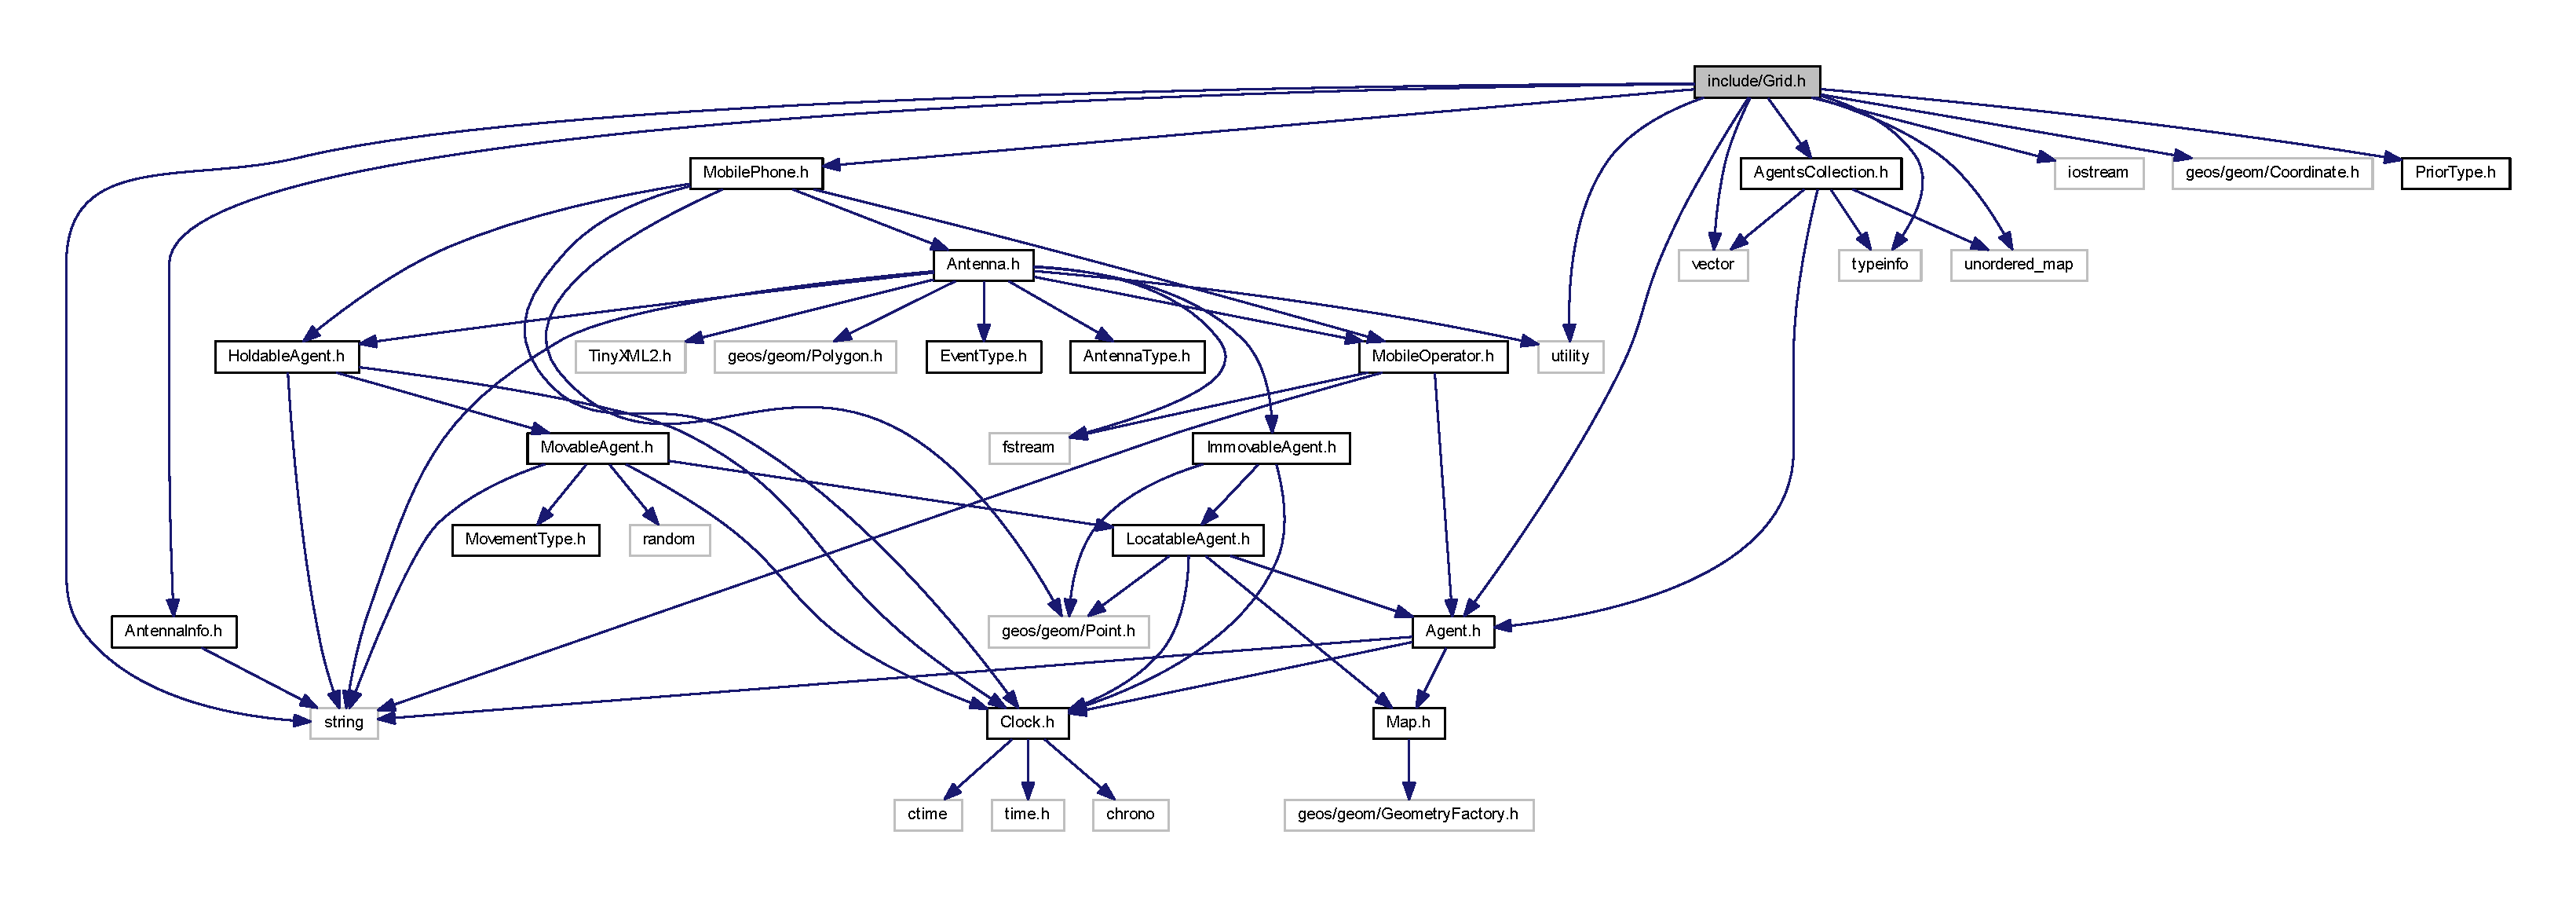
\includegraphics[width=350pt]{_grid_8h__incl}
\end{center}
\end{figure}
This graph shows which files directly or indirectly include this file\+:
\nopagebreak
\begin{figure}[H]
\begin{center}
\leavevmode
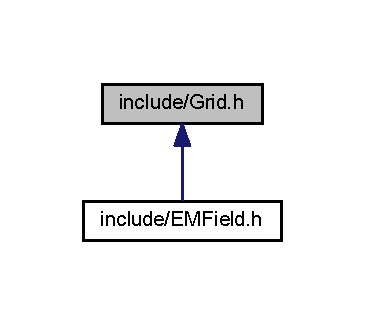
\includegraphics[width=350pt]{_grid_8h__dep__incl}
\end{center}
\end{figure}
\subsection*{Classes}
\begin{DoxyCompactItemize}
\item 
class \hyperlink{class_grid}{Grid}
\end{DoxyCompactItemize}

\section{include/\+Holdable\+Agent.h File Reference}
\label{_holdable_agent_8h}\index{include/HoldableAgent.h@{include/HoldableAgent.h}}
{\ttfamily \#include $<$Movable\+Agent.\+h$>$}\newline
{\ttfamily \#include $<$Clock.\+h$>$}\newline
{\ttfamily \#include $<$string$>$}\newline
\subsection*{Classes}
\begin{DoxyCompactItemize}
\item 
class \textbf{ Holdable\+Agent}
\end{DoxyCompactItemize}

\hypertarget{_i_d_generator_8h}{}\section{include/\+I\+D\+Generator.h File Reference}
\label{_i_d_generator_8h}\index{include/\+I\+D\+Generator.\+h@{include/\+I\+D\+Generator.\+h}}
\subsection*{Classes}
\begin{DoxyCompactItemize}
\item 
class \hyperlink{class_i_d_generator}{I\+D\+Generator}
\end{DoxyCompactItemize}

\hypertarget{_immovable_agent_8h}{}\section{include/\+Immovable\+Agent.h File Reference}
\label{_immovable_agent_8h}\index{include/ImmovableAgent.h@{include/ImmovableAgent.h}}
{\ttfamily \#include \char`\"{}Locatable\+Agent.\+h\char`\"{}}\newline
{\ttfamily \#include $<$Clock.\+h$>$}\newline
{\ttfamily \#include $<$geos/geom/\+Point.\+h$>$}\newline
Include dependency graph for Immovable\+Agent.\+h\+:\nopagebreak
\begin{figure}[H]
\begin{center}
\leavevmode
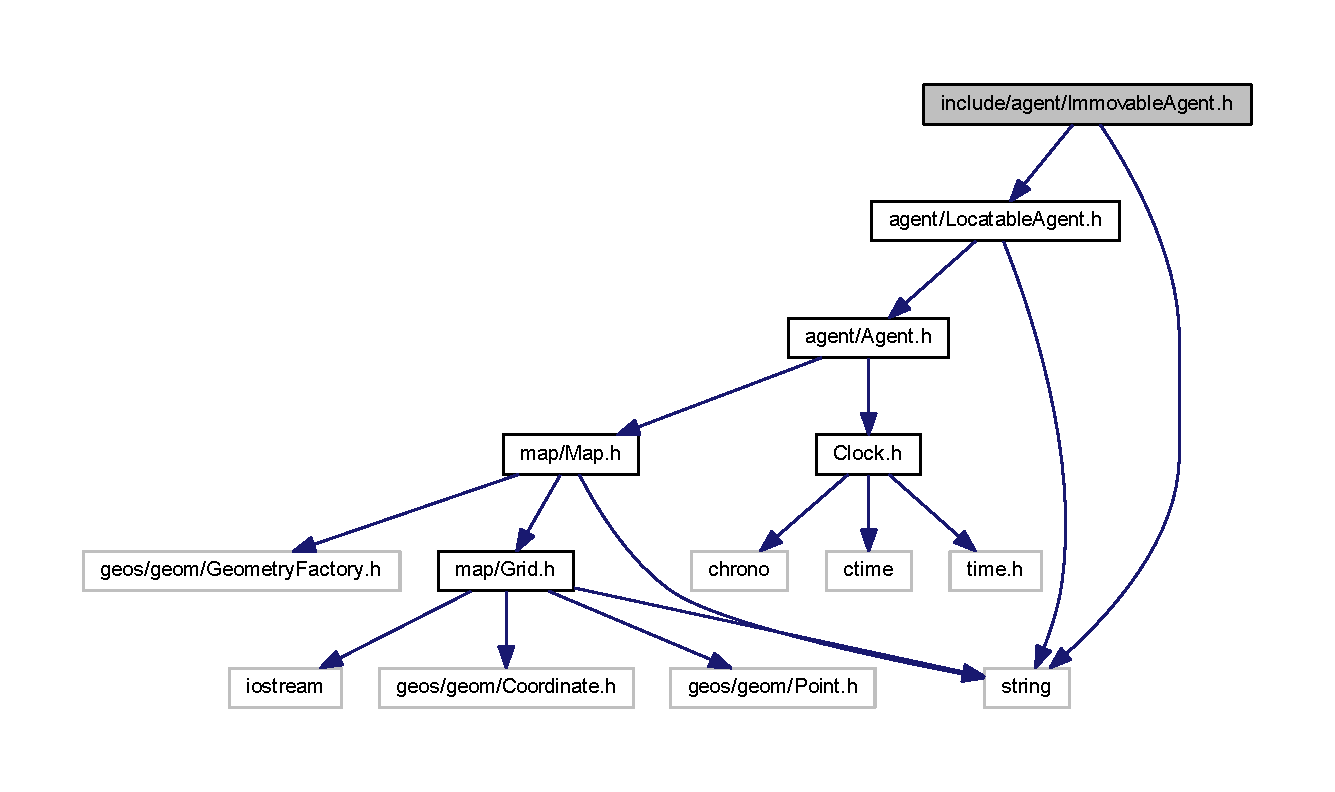
\includegraphics[width=350pt]{_immovable_agent_8h__incl}
\end{center}
\end{figure}
This graph shows which files directly or indirectly include this file\+:\nopagebreak
\begin{figure}[H]
\begin{center}
\leavevmode
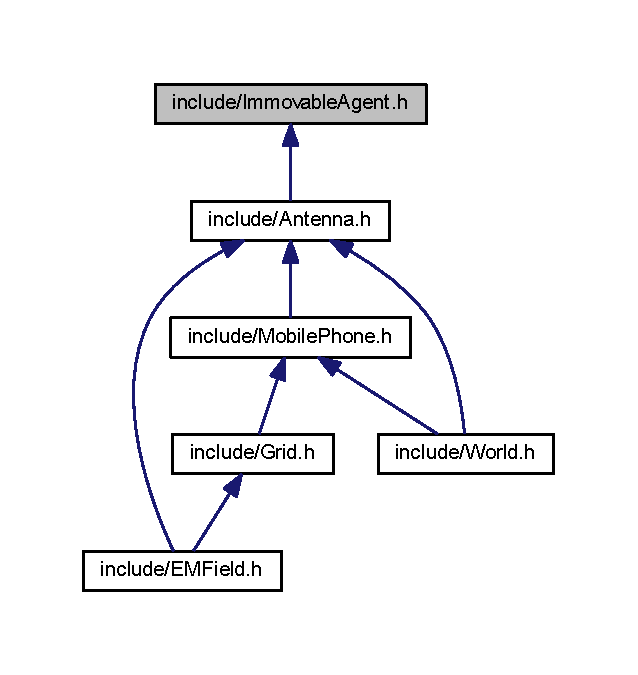
\includegraphics[width=309pt]{_immovable_agent_8h__dep__incl}
\end{center}
\end{figure}
\subsection*{Classes}
\begin{DoxyCompactItemize}
\item 
class \mbox{\hyperlink{class_immovable_agent}{Immovable\+Agent}}
\end{DoxyCompactItemize}

\section{include/\+Input\+Parser.h File Reference}
\label{_input_parser_8h}\index{include/InputParser.h@{include/InputParser.h}}
{\ttfamily \#include $<$string$>$}\newline
{\ttfamily \#include $<$vector$>$}\newline
\subsection*{Classes}
\begin{DoxyCompactItemize}
\item 
class \textbf{ Input\+Parser}
\end{DoxyCompactItemize}

\hypertarget{_locatable_agent_8h}{}\section{include/agent/\+Locatable\+Agent.h File Reference}
\label{_locatable_agent_8h}\index{include/agent/\+Locatable\+Agent.\+h@{include/agent/\+Locatable\+Agent.\+h}}
{\ttfamily \#include $<$agent/\+Agent.\+h$>$}\newline
{\ttfamily \#include $<$string$>$}\newline
Include dependency graph for Locatable\+Agent.\+h\+:
\nopagebreak
\begin{figure}[H]
\begin{center}
\leavevmode
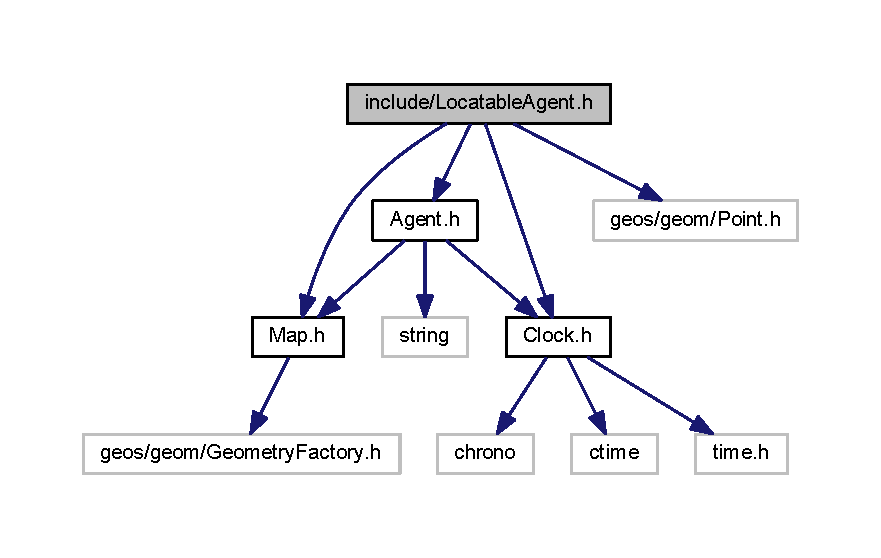
\includegraphics[width=350pt]{_locatable_agent_8h__incl}
\end{center}
\end{figure}
This graph shows which files directly or indirectly include this file\+:
\nopagebreak
\begin{figure}[H]
\begin{center}
\leavevmode
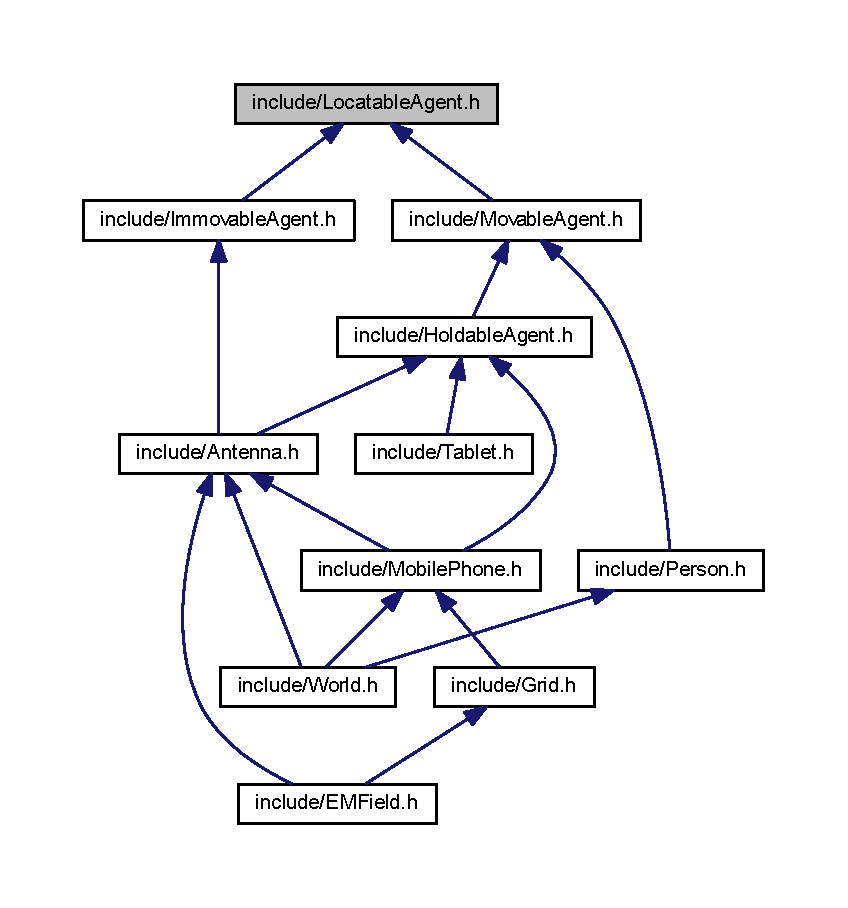
\includegraphics[width=350pt]{_locatable_agent_8h__dep__incl}
\end{center}
\end{figure}
\subsection*{Classes}
\begin{DoxyCompactItemize}
\item 
class \hyperlink{class_locatable_agent}{Locatable\+Agent}
\end{DoxyCompactItemize}

\hypertarget{_map_8h}{}\section{include/\+Map.h File Reference}
\label{_map_8h}\index{include/Map.h@{include/Map.h}}
{\ttfamily \#include $<$geos/geom/\+Geometry\+Factory.\+h$>$}\newline
Include dependency graph for Map.\+h\+:
\nopagebreak
\begin{figure}[H]
\begin{center}
\leavevmode
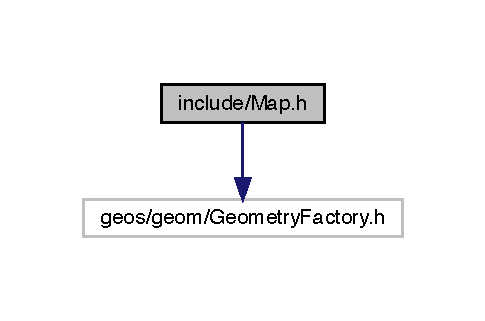
\includegraphics[width=233pt]{_map_8h__incl}
\end{center}
\end{figure}
This graph shows which files directly or indirectly include this file\+:
\nopagebreak
\begin{figure}[H]
\begin{center}
\leavevmode
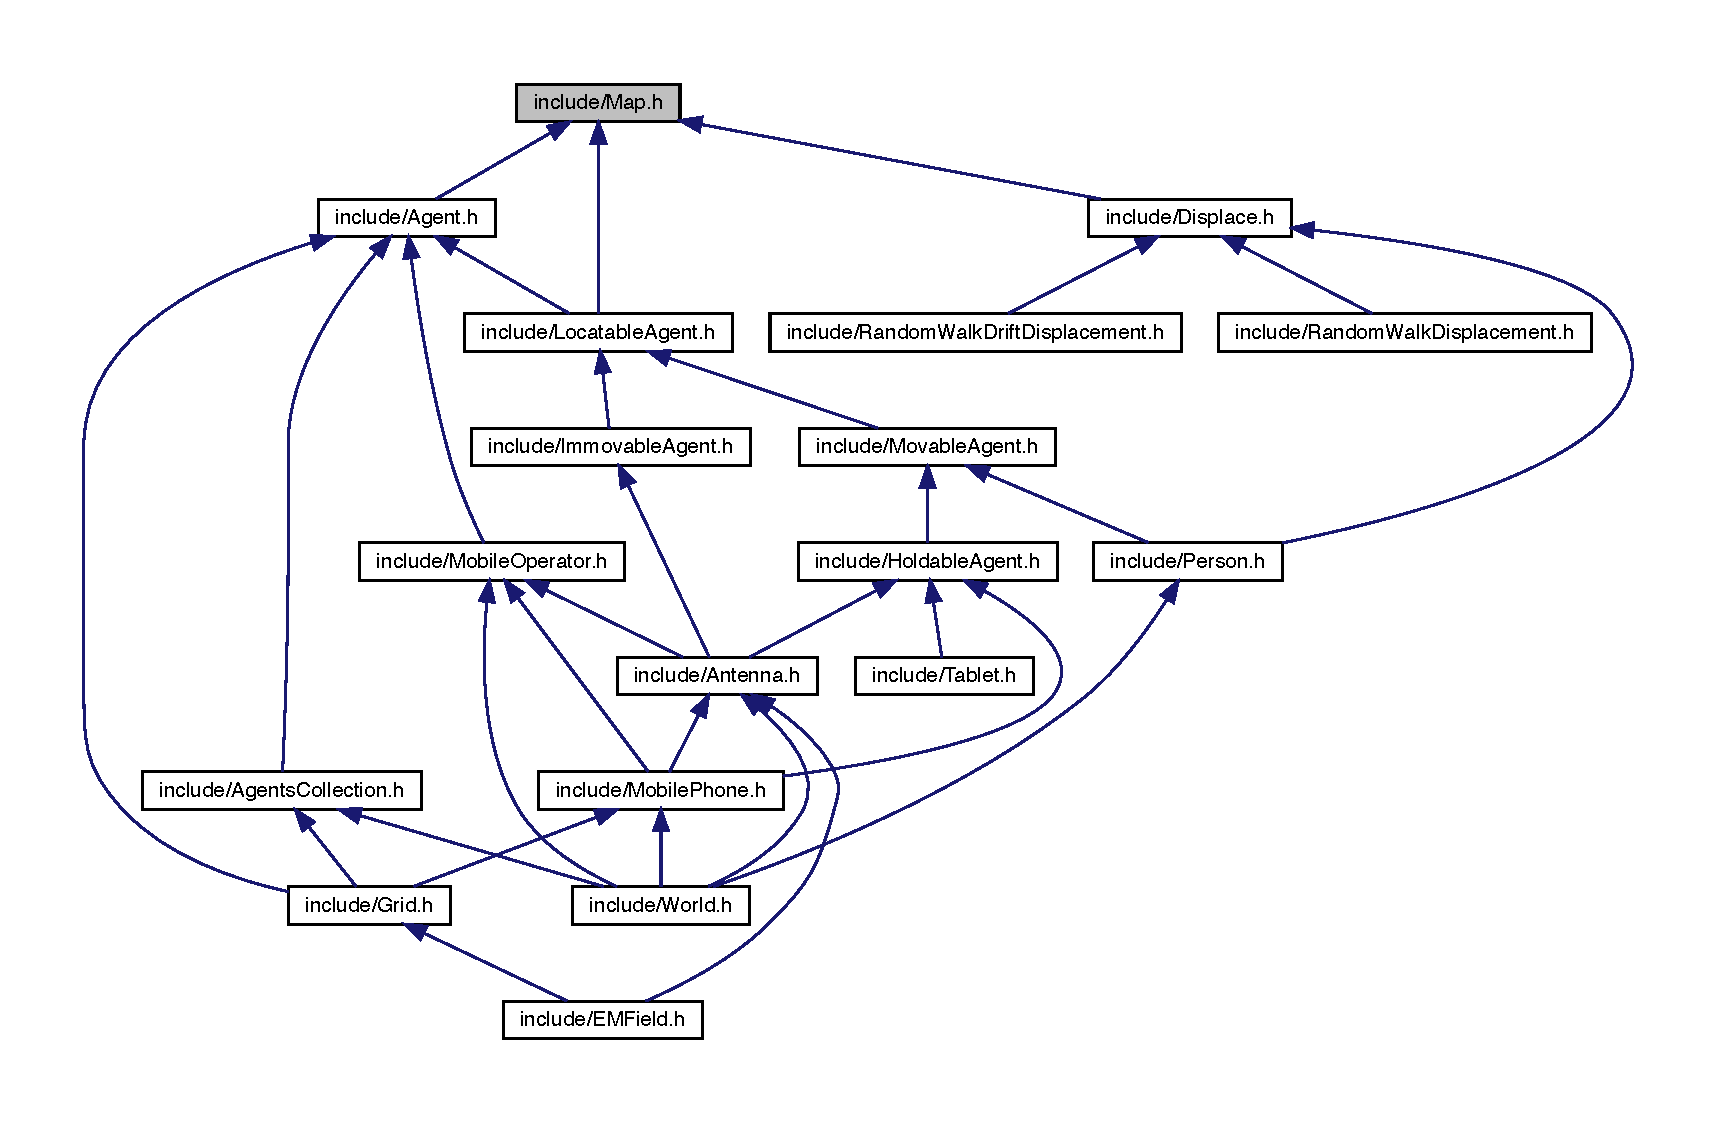
\includegraphics[width=350pt]{_map_8h__dep__incl}
\end{center}
\end{figure}
\subsection*{Classes}
\begin{DoxyCompactItemize}
\item 
class \mbox{\hyperlink{class_map}{Map}}
\end{DoxyCompactItemize}

\section{include/\+Mobile\+Phone.h File Reference}
\label{_mobile_phone_8h}\index{include/\+Mobile\+Phone.\+h@{include/\+Mobile\+Phone.\+h}}
{\ttfamily \#include $<$Holdable\+Agent.\+h$>$}\newline
{\ttfamily \#include $<$Antenna.\+h$>$}\newline
{\ttfamily \#include $<$Clock.\+h$>$}\newline
{\ttfamily \#include $<$geos/geom/\+Point.\+h$>$}\newline
Include dependency graph for Mobile\+Phone.\+h\+:
% FIG 0
This graph shows which files directly or indirectly include this file\+:
% FIG 1
\subsection*{Classes}
\begin{DoxyCompactItemize}
\item 
class \textbf{ Mobile\+Phone}
\end{DoxyCompactItemize}

\hypertarget{_movable_agent_8h}{}\section{include/\+Movable\+Agent.h File Reference}
\label{_movable_agent_8h}\index{include/MovableAgent.h@{include/MovableAgent.h}}
{\ttfamily \#include $<$Locatable\+Agent.\+h$>$}\newline
{\ttfamily \#include $<$Clock.\+h$>$}\newline
{\ttfamily \#include $<$random$>$}\newline
{\ttfamily \#include $<$Movement\+Type.\+h$>$}\newline
{\ttfamily \#include $<$string$>$}\newline
Include dependency graph for Movable\+Agent.\+h\+:
\nopagebreak
\begin{figure}[H]
\begin{center}
\leavevmode
\includegraphics[width=350pt]{_movable_agent_8h__incl}
\end{center}
\end{figure}
This graph shows which files directly or indirectly include this file\+:
\nopagebreak
\begin{figure}[H]
\begin{center}
\leavevmode
\includegraphics[width=350pt]{_movable_agent_8h__dep__incl}
\end{center}
\end{figure}
\subsection*{Classes}
\begin{DoxyCompactItemize}
\item 
class \mbox{\hyperlink{class_movable_agent}{Movable\+Agent}}
\end{DoxyCompactItemize}

\hypertarget{_movement_type_8h}{}\section{include/\+Movement\+Type.h File Reference}
\label{_movement_type_8h}\index{include/MovementType.h@{include/MovementType.h}}
This graph shows which files directly or indirectly include this file\+:\nopagebreak
\begin{figure}[H]
\begin{center}
\leavevmode
\includegraphics[width=350pt]{_movement_type_8h__dep__incl}
\end{center}
\end{figure}
\subsection*{Enumerations}
\begin{DoxyCompactItemize}
\item 
enum \mbox{\hyperlink{_movement_type_8h_a8a93b61bc797a7d1907f42796a252493}{Movement\+Type}} \{ \mbox{\hyperlink{_movement_type_8h_a8a93b61bc797a7d1907f42796a252493a1260a39bdcc19395a0085be09746f9d0}{Movement\+Type\+::\+R\+A\+N\+D\+O\+M\+\_\+\+W\+A\+L\+K\+\_\+\+C\+L\+O\+S\+E\+D\+\_\+\+M\+AP}}, 
\mbox{\hyperlink{_movement_type_8h_a8a93b61bc797a7d1907f42796a252493a19d5a14b0e46bf765f243b7e2b7b8810}{Movement\+Type\+::\+R\+A\+N\+D\+O\+M\+\_\+\+W\+A\+L\+K\+\_\+\+C\+L\+O\+S\+E\+D\+\_\+\+M\+A\+P\+\_\+\+W\+I\+T\+H\+\_\+\+D\+R\+I\+FT}}, 
\mbox{\hyperlink{_movement_type_8h_a8a93b61bc797a7d1907f42796a252493a696b031073e74bf2cb98e5ef201d4aa3}{Movement\+Type\+::\+U\+N\+K\+N\+O\+WN}}
 \}
\end{DoxyCompactItemize}


\subsection{Enumeration Type Documentation}
\mbox{\Hypertarget{_movement_type_8h_a8a93b61bc797a7d1907f42796a252493}\label{_movement_type_8h_a8a93b61bc797a7d1907f42796a252493}} 
\index{MovementType.h@{MovementType.h}!MovementType@{MovementType}}
\index{MovementType@{MovementType}!MovementType.h@{MovementType.h}}
\subsubsection{\texorpdfstring{MovementType}{MovementType}}
{\footnotesize\ttfamily enum \mbox{\hyperlink{_movement_type_8h_a8a93b61bc797a7d1907f42796a252493}{Movement\+Type}}\hspace{0.3cm}{\ttfamily [strong]}}

An enum class that enumerates the types of the methods used to move the people on the map. R\+A\+N\+D\+O\+M\+\_\+\+W\+A\+L\+K\+\_\+\+C\+L\+O\+S\+E\+D\+\_\+\+M\+AP -\/ the agent moves randomly inside the map boundary. The direction is generated as a random value at each time step and the step length is computed multiplying the speed with the time interval. R\+A\+N\+D\+O\+M\+\_\+\+W\+A\+L\+K\+\_\+\+C\+L\+O\+S\+E\+D\+\_\+\+M\+A\+P\+\_\+\+W\+I\+T\+H\+\_\+\+D\+R\+I\+FT\+: the agent moves in a preferential direction. There are two constants defining these directions\+: S\+I\+M\+\_\+\+T\+R\+E\+N\+D\+\_\+\+A\+N\+G\+L\+E\+\_\+1 and S\+I\+M\+\_\+\+T\+R\+E\+N\+D\+\_\+\+A\+N\+G\+L\+E\+\_\+2 (3P\+I/4 and 5P\+I/4). The actual direction is generated as a normally distributed random value with means equals to these constants and sad = 0.\+1. \begin{DoxyEnumFields}{Enumerator}
\raisebox{\heightof{T}}[0pt][0pt]{\index{RANDOM\_WALK\_CLOSED\_MAP@{RANDOM\_WALK\_CLOSED\_MAP}!MovementType.h@{MovementType.h}}\index{MovementType.h@{MovementType.h}!RANDOM\_WALK\_CLOSED\_MAP@{RANDOM\_WALK\_CLOSED\_MAP}}}\mbox{\Hypertarget{_movement_type_8h_a8a93b61bc797a7d1907f42796a252493a1260a39bdcc19395a0085be09746f9d0}\label{_movement_type_8h_a8a93b61bc797a7d1907f42796a252493a1260a39bdcc19395a0085be09746f9d0}} 
R\+A\+N\+D\+O\+M\+\_\+\+W\+A\+L\+K\+\_\+\+C\+L\+O\+S\+E\+D\+\_\+\+M\+AP&\\
\hline

\raisebox{\heightof{T}}[0pt][0pt]{\index{RANDOM\_WALK\_CLOSED\_MAP\_WITH\_DRIFT@{RANDOM\_WALK\_CLOSED\_MAP\_WITH\_DRIFT}!MovementType.h@{MovementType.h}}\index{MovementType.h@{MovementType.h}!RANDOM\_WALK\_CLOSED\_MAP\_WITH\_DRIFT@{RANDOM\_WALK\_CLOSED\_MAP\_WITH\_DRIFT}}}\mbox{\Hypertarget{_movement_type_8h_a8a93b61bc797a7d1907f42796a252493a19d5a14b0e46bf765f243b7e2b7b8810}\label{_movement_type_8h_a8a93b61bc797a7d1907f42796a252493a19d5a14b0e46bf765f243b7e2b7b8810}} 
R\+A\+N\+D\+O\+M\+\_\+\+W\+A\+L\+K\+\_\+\+C\+L\+O\+S\+E\+D\+\_\+\+M\+A\+P\+\_\+\+W\+I\+T\+H\+\_\+\+D\+R\+I\+FT&\\
\hline

\raisebox{\heightof{T}}[0pt][0pt]{\index{UNKNOWN@{UNKNOWN}!MovementType.h@{MovementType.h}}\index{MovementType.h@{MovementType.h}!UNKNOWN@{UNKNOWN}}}\mbox{\Hypertarget{_movement_type_8h_a8a93b61bc797a7d1907f42796a252493a696b031073e74bf2cb98e5ef201d4aa3}\label{_movement_type_8h_a8a93b61bc797a7d1907f42796a252493a696b031073e74bf2cb98e5ef201d4aa3}} 
U\+N\+K\+N\+O\+WN&\\
\hline

\end{DoxyEnumFields}

\hypertarget{_person_8h}{}\section{include/\+Person.h File Reference}
\label{_person_8h}\index{include/\+Person.\+h@{include/\+Person.\+h}}
{\ttfamily \#include $<$Movable\+Agent.\+h$>$}\newline
{\ttfamily \#include $<$geos/geom/\+Point.\+h$>$}\newline
{\ttfamily \#include $<$string$>$}\newline
{\ttfamily \#include $<$unordered\+\_\+map$>$}\newline
{\ttfamily \#include $<$Displace.\+h$>$}\newline
Include dependency graph for Person.\+h\+:\nopagebreak
\begin{figure}[H]
\begin{center}
\leavevmode
\includegraphics[width=350pt]{_person_8h__incl}
\end{center}
\end{figure}
This graph shows which files directly or indirectly include this file\+:\nopagebreak
\begin{figure}[H]
\begin{center}
\leavevmode
\includegraphics[width=169pt]{_person_8h__dep__incl}
\end{center}
\end{figure}
\subsection*{Classes}
\begin{DoxyCompactItemize}
\item 
class \hyperlink{class_person}{Person}
\end{DoxyCompactItemize}

\hypertarget{_random_number_generator_8h}{}\section{include/\+Random\+Number\+Generator.h File Reference}
\label{_random_number_generator_8h}\index{include/\+Random\+Number\+Generator.\+h@{include/\+Random\+Number\+Generator.\+h}}
{\ttfamily \#include $<$algorithm$>$}\newline
{\ttfamily \#include $<$random$>$}\newline
Include dependency graph for Random\+Number\+Generator.\+h\+:\nopagebreak
\begin{figure}[H]
\begin{center}
\leavevmode
\includegraphics[width=251pt]{_random_number_generator_8h__incl}
\end{center}
\end{figure}
\subsection*{Classes}
\begin{DoxyCompactItemize}
\item 
class \hyperlink{class_random_number_generator}{Random\+Number\+Generator}
\end{DoxyCompactItemize}

\hypertarget{_tablet_8h}{}\section{include/\+Tablet.h File Reference}
\label{_tablet_8h}\index{include/\+Tablet.\+h@{include/\+Tablet.\+h}}
{\ttfamily \#include $<$Holdable\+Agent.\+h$>$}\newline
{\ttfamily \#include $<$Movement\+Type.\+h$>$}\newline
Include dependency graph for Tablet.\+h\+:\nopagebreak
\begin{figure}[H]
\begin{center}
\leavevmode
\includegraphics[width=350pt]{_tablet_8h__incl}
\end{center}
\end{figure}
\subsection*{Classes}
\begin{DoxyCompactItemize}
\item 
class \hyperlink{class_tablet}{Tablet}
\end{DoxyCompactItemize}

\section{include/tinyxml2.h File Reference}
\label{tinyxml2_8h}\index{include/tinyxml2.\+h@{include/tinyxml2.\+h}}
{\ttfamily \#include $<$cctype$>$}\newline
{\ttfamily \#include $<$climits$>$}\newline
{\ttfamily \#include $<$cstdio$>$}\newline
{\ttfamily \#include $<$cstdlib$>$}\newline
{\ttfamily \#include $<$cstring$>$}\newline
{\ttfamily \#include $<$stdint.\+h$>$}\newline
Include dependency graph for tinyxml2.\+h\+:
% FIG 0
This graph shows which files directly or indirectly include this file\+:
% FIG 1
\subsection*{Classes}
\begin{DoxyCompactItemize}
\item 
class \textbf{ tinyxml2\+::\+Str\+Pair}
\item 
class \textbf{ tinyxml2\+::\+Dyn\+Array$<$ T, I\+N\+I\+T\+I\+A\+L\+\_\+\+S\+I\+Z\+E $>$}
\item 
class \textbf{ tinyxml2\+::\+Mem\+Pool}
\item 
class \textbf{ tinyxml2\+::\+Mem\+Pool\+T$<$ I\+T\+E\+M\+\_\+\+S\+I\+Z\+E $>$}
\item 
union \textbf{ tinyxml2\+::\+Mem\+Pool\+T$<$ I\+T\+E\+M\+\_\+\+S\+I\+Z\+E $>$\+::\+Item}
\item 
struct \textbf{ tinyxml2\+::\+Mem\+Pool\+T$<$ I\+T\+E\+M\+\_\+\+S\+I\+Z\+E $>$\+::\+Block}
\item 
class \textbf{ tinyxml2\+::\+X\+M\+L\+Visitor}
\item 
class \textbf{ tinyxml2\+::\+X\+M\+L\+Util}
\item 
class \textbf{ tinyxml2\+::\+X\+M\+L\+Node}
\item 
class \textbf{ tinyxml2\+::\+X\+M\+L\+Text}
\item 
class \textbf{ tinyxml2\+::\+X\+M\+L\+Comment}
\item 
class \textbf{ tinyxml2\+::\+X\+M\+L\+Declaration}
\item 
class \textbf{ tinyxml2\+::\+X\+M\+L\+Unknown}
\item 
class \textbf{ tinyxml2\+::\+X\+M\+L\+Attribute}
\item 
class \textbf{ tinyxml2\+::\+X\+M\+L\+Element}
\item 
class \textbf{ tinyxml2\+::\+X\+M\+L\+Document}
\item 
class \textbf{ tinyxml2\+::\+X\+M\+L\+Document\+::\+Depth\+Tracker}
\item 
class \textbf{ tinyxml2\+::\+X\+M\+L\+Handle}
\item 
class \textbf{ tinyxml2\+::\+X\+M\+L\+Const\+Handle}
\item 
class \textbf{ tinyxml2\+::\+X\+M\+L\+Printer}
\end{DoxyCompactItemize}
\subsection*{Namespaces}
\begin{DoxyCompactItemize}
\item 
 \textbf{ tinyxml2}
\end{DoxyCompactItemize}
\subsection*{Macros}
\begin{DoxyCompactItemize}
\item 
\#define \textbf{ T\+I\+N\+Y\+X\+M\+L2\+\_\+\+L\+IB}
\item 
\#define \textbf{ T\+I\+X\+M\+L\+A\+S\+S\+E\+RT}(x)~\{\}
\item 
\#define \textbf{ T\+I\+N\+Y\+X\+M\+L2\+\_\+\+M\+A\+J\+O\+R\+\_\+\+V\+E\+R\+S\+I\+ON}~7
\item 
\#define \textbf{ T\+I\+N\+Y\+X\+M\+L2\+\_\+\+M\+I\+N\+O\+R\+\_\+\+V\+E\+R\+S\+I\+ON}~0
\item 
\#define \textbf{ T\+I\+N\+Y\+X\+M\+L2\+\_\+\+P\+A\+T\+C\+H\+\_\+\+V\+E\+R\+S\+I\+ON}~1
\end{DoxyCompactItemize}
\subsection*{Enumerations}
\begin{DoxyCompactItemize}
\item 
enum \textbf{ tinyxml2\+::\+X\+M\+L\+Error} \{ \newline
\textbf{ tinyxml2\+::\+X\+M\+L\+\_\+\+S\+U\+C\+C\+E\+SS} = 0, 
\textbf{ tinyxml2\+::\+X\+M\+L\+\_\+\+N\+O\+\_\+\+A\+T\+T\+R\+I\+B\+U\+TE}, 
\textbf{ tinyxml2\+::\+X\+M\+L\+\_\+\+W\+R\+O\+N\+G\+\_\+\+A\+T\+T\+R\+I\+B\+U\+T\+E\+\_\+\+T\+Y\+PE}, 
\textbf{ tinyxml2\+::\+X\+M\+L\+\_\+\+E\+R\+R\+O\+R\+\_\+\+F\+I\+L\+E\+\_\+\+N\+O\+T\+\_\+\+F\+O\+U\+ND}, 
\newline
\textbf{ tinyxml2\+::\+X\+M\+L\+\_\+\+E\+R\+R\+O\+R\+\_\+\+F\+I\+L\+E\+\_\+\+C\+O\+U\+L\+D\+\_\+\+N\+O\+T\+\_\+\+B\+E\+\_\+\+O\+P\+E\+N\+ED}, 
\textbf{ tinyxml2\+::\+X\+M\+L\+\_\+\+E\+R\+R\+O\+R\+\_\+\+F\+I\+L\+E\+\_\+\+R\+E\+A\+D\+\_\+\+E\+R\+R\+OR}, 
\textbf{ tinyxml2\+::\+X\+M\+L\+\_\+\+E\+R\+R\+O\+R\+\_\+\+P\+A\+R\+S\+I\+N\+G\+\_\+\+E\+L\+E\+M\+E\+NT}, 
\textbf{ tinyxml2\+::\+X\+M\+L\+\_\+\+E\+R\+R\+O\+R\+\_\+\+P\+A\+R\+S\+I\+N\+G\+\_\+\+A\+T\+T\+R\+I\+B\+U\+TE}, 
\newline
\textbf{ tinyxml2\+::\+X\+M\+L\+\_\+\+E\+R\+R\+O\+R\+\_\+\+P\+A\+R\+S\+I\+N\+G\+\_\+\+T\+E\+XT}, 
\textbf{ tinyxml2\+::\+X\+M\+L\+\_\+\+E\+R\+R\+O\+R\+\_\+\+P\+A\+R\+S\+I\+N\+G\+\_\+\+C\+D\+A\+TA}, 
\textbf{ tinyxml2\+::\+X\+M\+L\+\_\+\+E\+R\+R\+O\+R\+\_\+\+P\+A\+R\+S\+I\+N\+G\+\_\+\+C\+O\+M\+M\+E\+NT}, 
\textbf{ tinyxml2\+::\+X\+M\+L\+\_\+\+E\+R\+R\+O\+R\+\_\+\+P\+A\+R\+S\+I\+N\+G\+\_\+\+D\+E\+C\+L\+A\+R\+A\+T\+I\+ON}, 
\newline
\textbf{ tinyxml2\+::\+X\+M\+L\+\_\+\+E\+R\+R\+O\+R\+\_\+\+P\+A\+R\+S\+I\+N\+G\+\_\+\+U\+N\+K\+N\+O\+WN}, 
\textbf{ tinyxml2\+::\+X\+M\+L\+\_\+\+E\+R\+R\+O\+R\+\_\+\+E\+M\+P\+T\+Y\+\_\+\+D\+O\+C\+U\+M\+E\+NT}, 
\textbf{ tinyxml2\+::\+X\+M\+L\+\_\+\+E\+R\+R\+O\+R\+\_\+\+M\+I\+S\+M\+A\+T\+C\+H\+E\+D\+\_\+\+E\+L\+E\+M\+E\+NT}, 
\textbf{ tinyxml2\+::\+X\+M\+L\+\_\+\+E\+R\+R\+O\+R\+\_\+\+P\+A\+R\+S\+I\+NG}, 
\newline
\textbf{ tinyxml2\+::\+X\+M\+L\+\_\+\+C\+A\+N\+\_\+\+N\+O\+T\+\_\+\+C\+O\+N\+V\+E\+R\+T\+\_\+\+T\+E\+XT}, 
\textbf{ tinyxml2\+::\+X\+M\+L\+\_\+\+N\+O\+\_\+\+T\+E\+X\+T\+\_\+\+N\+O\+DE}, 
\textbf{ tinyxml2\+::\+X\+M\+L\+\_\+\+E\+L\+E\+M\+E\+N\+T\+\_\+\+D\+E\+P\+T\+H\+\_\+\+E\+X\+C\+E\+E\+D\+ED}, 
\textbf{ tinyxml2\+::\+X\+M\+L\+\_\+\+E\+R\+R\+O\+R\+\_\+\+C\+O\+U\+NT}
 \}
\item 
enum \textbf{ tinyxml2\+::\+Whitespace} \{ \textbf{ tinyxml2\+::\+P\+R\+E\+S\+E\+R\+V\+E\+\_\+\+W\+H\+I\+T\+E\+S\+P\+A\+CE}, 
\textbf{ tinyxml2\+::\+C\+O\+L\+L\+A\+P\+S\+E\+\_\+\+W\+H\+I\+T\+E\+S\+P\+A\+CE}
 \}
\end{DoxyCompactItemize}


\subsection{Macro Definition Documentation}
\mbox{\label{tinyxml2_8h_a8953517b8490d756ad0bfef40fe5811f}} 
\index{tinyxml2.\+h@{tinyxml2.\+h}!T\+I\+N\+Y\+X\+M\+L2\+\_\+\+L\+IB@{T\+I\+N\+Y\+X\+M\+L2\+\_\+\+L\+IB}}
\index{T\+I\+N\+Y\+X\+M\+L2\+\_\+\+L\+IB@{T\+I\+N\+Y\+X\+M\+L2\+\_\+\+L\+IB}!tinyxml2.\+h@{tinyxml2.\+h}}
\subsubsection{T\+I\+N\+Y\+X\+M\+L2\+\_\+\+L\+IB}
{\footnotesize\ttfamily \#define T\+I\+N\+Y\+X\+M\+L2\+\_\+\+L\+IB}



Definition at line 78 of file tinyxml2.\+h.

\mbox{\label{tinyxml2_8h_a530d8240c8e91a9ba8b8dae2d0024571}} 
\index{tinyxml2.\+h@{tinyxml2.\+h}!T\+I\+N\+Y\+X\+M\+L2\+\_\+\+M\+A\+J\+O\+R\+\_\+\+V\+E\+R\+S\+I\+ON@{T\+I\+N\+Y\+X\+M\+L2\+\_\+\+M\+A\+J\+O\+R\+\_\+\+V\+E\+R\+S\+I\+ON}}
\index{T\+I\+N\+Y\+X\+M\+L2\+\_\+\+M\+A\+J\+O\+R\+\_\+\+V\+E\+R\+S\+I\+ON@{T\+I\+N\+Y\+X\+M\+L2\+\_\+\+M\+A\+J\+O\+R\+\_\+\+V\+E\+R\+S\+I\+ON}!tinyxml2.\+h@{tinyxml2.\+h}}
\subsubsection{T\+I\+N\+Y\+X\+M\+L2\+\_\+\+M\+A\+J\+O\+R\+\_\+\+V\+E\+R\+S\+I\+ON}
{\footnotesize\ttfamily \#define T\+I\+N\+Y\+X\+M\+L2\+\_\+\+M\+A\+J\+O\+R\+\_\+\+V\+E\+R\+S\+I\+ON~7}



Definition at line 105 of file tinyxml2.\+h.

\mbox{\label{tinyxml2_8h_ae81f14093bb46006bfba7bbb874f2ad7}} 
\index{tinyxml2.\+h@{tinyxml2.\+h}!T\+I\+N\+Y\+X\+M\+L2\+\_\+\+M\+I\+N\+O\+R\+\_\+\+V\+E\+R\+S\+I\+ON@{T\+I\+N\+Y\+X\+M\+L2\+\_\+\+M\+I\+N\+O\+R\+\_\+\+V\+E\+R\+S\+I\+ON}}
\index{T\+I\+N\+Y\+X\+M\+L2\+\_\+\+M\+I\+N\+O\+R\+\_\+\+V\+E\+R\+S\+I\+ON@{T\+I\+N\+Y\+X\+M\+L2\+\_\+\+M\+I\+N\+O\+R\+\_\+\+V\+E\+R\+S\+I\+ON}!tinyxml2.\+h@{tinyxml2.\+h}}
\subsubsection{T\+I\+N\+Y\+X\+M\+L2\+\_\+\+M\+I\+N\+O\+R\+\_\+\+V\+E\+R\+S\+I\+ON}
{\footnotesize\ttfamily \#define T\+I\+N\+Y\+X\+M\+L2\+\_\+\+M\+I\+N\+O\+R\+\_\+\+V\+E\+R\+S\+I\+ON~0}



Definition at line 106 of file tinyxml2.\+h.

\mbox{\label{tinyxml2_8h_ae01c0f3f1b45c29e71209555c5821afc}} 
\index{tinyxml2.\+h@{tinyxml2.\+h}!T\+I\+N\+Y\+X\+M\+L2\+\_\+\+P\+A\+T\+C\+H\+\_\+\+V\+E\+R\+S\+I\+ON@{T\+I\+N\+Y\+X\+M\+L2\+\_\+\+P\+A\+T\+C\+H\+\_\+\+V\+E\+R\+S\+I\+ON}}
\index{T\+I\+N\+Y\+X\+M\+L2\+\_\+\+P\+A\+T\+C\+H\+\_\+\+V\+E\+R\+S\+I\+ON@{T\+I\+N\+Y\+X\+M\+L2\+\_\+\+P\+A\+T\+C\+H\+\_\+\+V\+E\+R\+S\+I\+ON}!tinyxml2.\+h@{tinyxml2.\+h}}
\subsubsection{T\+I\+N\+Y\+X\+M\+L2\+\_\+\+P\+A\+T\+C\+H\+\_\+\+V\+E\+R\+S\+I\+ON}
{\footnotesize\ttfamily \#define T\+I\+N\+Y\+X\+M\+L2\+\_\+\+P\+A\+T\+C\+H\+\_\+\+V\+E\+R\+S\+I\+ON~1}



Definition at line 107 of file tinyxml2.\+h.

\mbox{\label{tinyxml2_8h_a029877acb3c6fd71698561044953bd14}} 
\index{tinyxml2.\+h@{tinyxml2.\+h}!T\+I\+X\+M\+L\+A\+S\+S\+E\+RT@{T\+I\+X\+M\+L\+A\+S\+S\+E\+RT}}
\index{T\+I\+X\+M\+L\+A\+S\+S\+E\+RT@{T\+I\+X\+M\+L\+A\+S\+S\+E\+RT}!tinyxml2.\+h@{tinyxml2.\+h}}
\subsubsection{T\+I\+X\+M\+L\+A\+S\+S\+E\+RT}
{\footnotesize\ttfamily \#define T\+I\+X\+M\+L\+A\+S\+S\+E\+RT(\begin{DoxyParamCaption}\item[{}]{x }\end{DoxyParamCaption})~\{\}}



Definition at line 94 of file tinyxml2.\+h.



Referenced by tinyxml2\+::\+X\+M\+L\+Text\+::\+Accept(), tinyxml2\+::\+X\+M\+L\+Comment\+::\+Accept(), tinyxml2\+::\+X\+M\+L\+Declaration\+::\+Accept(), tinyxml2\+::\+X\+M\+L\+Unknown\+::\+Accept(), tinyxml2\+::\+X\+M\+L\+Element\+::\+Accept(), tinyxml2\+::\+X\+M\+L\+Document\+::\+Accept(), tinyxml2\+::\+Mem\+Pool\+T$<$ sizeof(tinyxml2\+::\+X\+M\+L\+Element) $>$\+::\+Alloc(), tinyxml2\+::\+Dyn\+Array$<$ char, 20 $>$\+::\+Capacity(), tinyxml2\+::\+X\+M\+L\+Document\+::\+Clear(), tinyxml2\+::\+Str\+Pair\+::\+Collapse\+Whitespace(), tinyxml2\+::\+X\+M\+L\+Util\+::\+Convert\+U\+T\+F32\+To\+U\+T\+F8(), tinyxml2\+::\+X\+M\+L\+Element\+::\+Create\+Attribute(), tinyxml2\+::\+X\+M\+L\+Document\+::\+Create\+Unlinked\+Node(), tinyxml2\+::\+X\+M\+L\+Node\+::\+Deep\+Clone(), tinyxml2\+::\+X\+M\+L\+Document\+::\+Deep\+Copy(), tinyxml2\+::\+X\+M\+L\+Node\+::\+Delete\+Child(), tinyxml2\+::\+X\+M\+L\+Node\+::\+Delete\+Children(), tinyxml2\+::\+X\+M\+L\+Node\+::\+Delete\+Node(), tinyxml2\+::\+X\+M\+L\+Document\+::\+Delete\+Node(), tinyxml2\+::\+Dyn\+Array$<$ char, 20 $>$\+::\+Ensure\+Capacity(), tinyxml2\+::\+X\+M\+L\+Document\+::\+Error\+I\+D\+To\+Name(), tinyxml2\+::\+X\+M\+L\+Element\+::\+Find\+Or\+Create\+Attribute(), tinyxml2\+::\+X\+M\+L\+Util\+::\+Get\+Character\+Ref(), tinyxml2\+::\+X\+M\+L\+Node\+::\+Get\+Document(), tinyxml2\+::\+Str\+Pair\+::\+Get\+Str(), tinyxml2\+::\+X\+M\+L\+Document\+::\+Identify(), tinyxml2\+::\+X\+M\+L\+Node\+::\+Insert\+After\+Child(), tinyxml2\+::\+X\+M\+L\+Node\+::\+Insert\+Child\+Preamble(), tinyxml2\+::\+X\+M\+L\+Node\+::\+Insert\+End\+Child(), tinyxml2\+::\+X\+M\+L\+Node\+::\+Insert\+First\+Child(), tinyxml2\+::\+X\+M\+L\+Document\+::\+Load\+File(), tinyxml2\+::\+X\+M\+L\+Document\+::\+Mark\+In\+Use(), tinyxml2\+::\+Dyn\+Array$<$ char, 20 $>$\+::\+Mem(), tinyxml2\+::\+X\+M\+L\+Document\+::\+New\+Unknown(), tinyxml2\+::\+Dyn\+Array$<$ char, 20 $>$\+::operator[$\,$](), tinyxml2\+::\+X\+M\+L\+Document\+::\+Parse(), tinyxml2\+::\+X\+M\+L\+Element\+::\+Parse\+Attributes(), tinyxml2\+::\+X\+M\+L\+Node\+::\+Parse\+Deep(), tinyxml2\+::\+Str\+Pair\+::\+Parse\+Text(), tinyxml2\+::\+Dyn\+Array$<$ char, 20 $>$\+::\+Peek\+Top(), tinyxml2\+::\+Dyn\+Array$<$ char, 20 $>$\+::\+Pop(), tinyxml2\+::\+Dyn\+Array$<$ char, 20 $>$\+::\+Pop\+Arr(), tinyxml2\+::\+X\+M\+L\+Document\+::\+Pop\+Depth(), tinyxml2\+::\+X\+M\+L\+Printer\+::\+Print\+String(), tinyxml2\+::\+Dyn\+Array$<$ char, 20 $>$\+::\+Push(), tinyxml2\+::\+Dyn\+Array$<$ char, 20 $>$\+::\+Push\+Arr(), tinyxml2\+::\+X\+M\+L\+Printer\+::\+Push\+Attribute(), tinyxml2\+::\+X\+M\+L\+Util\+::\+Read\+B\+O\+M(), tinyxml2\+::\+X\+M\+L\+Document\+::\+Save\+File(), tinyxml2\+::\+Str\+Pair\+::\+Set(), tinyxml2\+::\+X\+M\+L\+Document\+::\+Set\+Error(), tinyxml2\+::\+Str\+Pair\+::\+Set\+Str(), tinyxml2\+::\+X\+M\+L\+Text\+::\+Shallow\+Equal(), tinyxml2\+::\+X\+M\+L\+Comment\+::\+Shallow\+Equal(), tinyxml2\+::\+X\+M\+L\+Declaration\+::\+Shallow\+Equal(), tinyxml2\+::\+X\+M\+L\+Unknown\+::\+Shallow\+Equal(), tinyxml2\+::\+X\+M\+L\+Element\+::\+Shallow\+Equal(), tinyxml2\+::\+Dyn\+Array$<$ char, 20 $>$\+::\+Size(), tinyxml2\+::\+X\+M\+L\+Util\+::\+Skip\+White\+Space(), tinyxml2\+::\+X\+M\+L\+Util\+::\+String\+Equal(), tinyxml2\+::\+Dyn\+Array$<$ char, 20 $>$\+::\+Swap\+Remove(), tinyxml2\+::\+X\+M\+L\+Document\+::\+To\+Document(), tinyxml2\+::\+Str\+Pair\+::\+Transfer\+To(), tinyxml2\+::\+X\+M\+L\+Node\+::\+Unlink(), and tinyxml2\+::\+X\+M\+L\+Printer\+::\+X\+M\+L\+Printer().


\section{include/\+T\+Norm.h File Reference}
\label{_t_norm_8h}\index{include/TNorm.h@{include/TNorm.h}}
\subsection*{Namespaces}
\begin{DoxyCompactItemize}
\item 
 \textbf{ Rtnorm}
\end{DoxyCompactItemize}
\subsection*{Variables}
\begin{DoxyCompactItemize}
\item 
static const double \textbf{ Rtnorm\+::x} [4002]
\item 
static const double \textbf{ Rtnorm\+::yu} [4001]
\item 
static const int \textbf{ Rtnorm\+::ncell} [8961]
\end{DoxyCompactItemize}

\section{include/\+Utils.h File Reference}
\label{_utils_8h}\index{include/\+Utils.\+h@{include/\+Utils.\+h}}
{\ttfamily \#include $<$geos/geom/\+Point.\+h$>$}\newline
{\ttfamily \#include $<$cmath$>$}\newline
{\ttfamily \#include $<$vector$>$}\newline
{\ttfamily \#include $<$tinyxml2.\+h$>$}\newline
Include dependency graph for Utils.\+h\+:
% FIG 0
This graph shows which files directly or indirectly include this file\+:
% FIG 1
\subsection*{Namespaces}
\begin{DoxyCompactItemize}
\item 
 \textbf{ utils}
\end{DoxyCompactItemize}
\subsection*{Functions}
\begin{DoxyCompactItemize}
\item 
vector$<$ Point $\ast$ $>$ \textbf{ utils\+::generate\+Points} (\textbf{ Map} $\ast$m, int n)
\item 
void \textbf{ utils\+::print\+Person\+Header} ()
\item 
void \textbf{ utils\+::print\+Antenna\+Header} ()
\item 
void \textbf{ utils\+::print\+Phone\+Header} ()
\item 
const char $\ast$ \textbf{ utils\+::get\+Antennas\+File} (int argc, char $\ast$$\ast$argv)
\item 
\textbf{ X\+M\+L\+Node} $\ast$ \textbf{ utils\+::get\+Node} (\textbf{ X\+M\+L\+Element} $\ast$el, const char $\ast$name)
\item 
\textbf{ X\+M\+L\+Element} $\ast$ \textbf{ utils\+::get\+First\+Child\+Element} (\textbf{ X\+M\+L\+Element} $\ast$el, const char $\ast$name) noexcept(false)
\end{DoxyCompactItemize}
\subsection*{Variables}
\begin{DoxyCompactItemize}
\item 
const double \textbf{ utils\+::\+PI} = std\+::atan(1.\+0) $\ast$ 4
\end{DoxyCompactItemize}

\section{include/\+World.h File Reference}
\label{_world_8h}\index{include/World.h@{include/World.h}}
{\ttfamily \#include $<$Antenna.\+h$>$}\newline
{\ttfamily \#include $<$Person.\+h$>$}\newline
{\ttfamily \#include $<$random$>$}\newline
{\ttfamily \#include $<$vector$>$}\newline
{\ttfamily \#include $<$Agents\+Collection.\+h$>$}\newline
{\ttfamily \#include $<$Clock.\+h$>$}\newline
{\ttfamily \#include $<$Mobile\+Phone.\+h$>$}\newline
{\ttfamily \#include $<$tinyxml2.\+h$>$}\newline
{\ttfamily \#include $<$Movement\+Type.\+h$>$}\newline
\subsection*{Classes}
\begin{DoxyCompactItemize}
\item 
class \textbf{ World}
\end{DoxyCompactItemize}

\section{src/\+Agent.cpp File Reference}
\label{_agent_8cpp}\index{src/\+Agent.\+cpp@{src/\+Agent.\+cpp}}
{\ttfamily \#include $<$Agent.\+h$>$}\newline
Include dependency graph for Agent.\+cpp\+:
% FIG 0

\section{src/\+Agents\+Collection.cpp File Reference}
\label{_agents_collection_8cpp}\index{src/\+Agents\+Collection.\+cpp@{src/\+Agents\+Collection.\+cpp}}
{\ttfamily \#include $<$Agents\+Collection.\+h$>$}\newline
{\ttfamily \#include $<$initializer\+\_\+list$>$}\newline
{\ttfamily \#include $<$iostream$>$}\newline
{\ttfamily \#include $<$utility$>$}\newline
Include dependency graph for Agents\+Collection.\+cpp\+:
% FIG 0

\section{src/\+Antenna.cpp File Reference}
\label{_antenna_8cpp}\index{src/\+Antenna.\+cpp@{src/\+Antenna.\+cpp}}
{\ttfamily \#include $<$Antenna.\+h$>$}\newline
{\ttfamily \#include $<$Holdable\+Agent.\+h$>$}\newline
{\ttfamily \#include $<$Event\+Type.\+h$>$}\newline
{\ttfamily \#include $<$Constants.\+h$>$}\newline
{\ttfamily \#include $<$geos/geom/\+Geometry\+Factory.\+h$>$}\newline
{\ttfamily \#include $<$Map.\+h$>$}\newline
{\ttfamily \#include $<$iomanip$>$}\newline
{\ttfamily \#include $<$sstream$>$}\newline
{\ttfamily \#include $<$fstream$>$}\newline
{\ttfamily \#include $<$algorithm$>$}\newline
{\ttfamily \#include $<$string$>$}\newline
{\ttfamily \#include $<$string.\+h$>$}\newline
{\ttfamily \#include $<$tinyxml2.\+h$>$}\newline
{\ttfamily \#include $<$Utils.\+h$>$}\newline
Include dependency graph for Antenna.\+cpp\+:
% FIG 0

\section{src/\+Antenna\+Info.cpp File Reference}
\label{_antenna_info_8cpp}\index{src/AntennaInfo.cpp@{src/AntennaInfo.cpp}}
{\ttfamily \#include $<$Antenna\+Info.\+h$>$}\newline
{\ttfamily \#include $<$string$>$}\newline
{\ttfamily \#include $<$sstream$>$}\newline

\section{src/\+Clock.cpp File Reference}
\label{_clock_8cpp}\index{src/Clock.cpp@{src/Clock.cpp}}
{\ttfamily \#include $<$Clock.\+h$>$}\newline
{\ttfamily \#include $<$ctime$>$}\newline

\section{src/\+Constants.cpp File Reference}
\label{_constants_8cpp}\index{src/Constants.cpp@{src/Constants.cpp}}
{\ttfamily \#include $<$Constants.\+h$>$}\newline

\section{src/\+C\+S\+V\+Parser.cpp File Reference}
\label{_c_s_v_parser_8cpp}\index{src/\+C\+S\+V\+Parser.\+cpp@{src/\+C\+S\+V\+Parser.\+cpp}}
{\ttfamily \#include $<$fstream$>$}\newline
{\ttfamily \#include $<$sstream$>$}\newline
{\ttfamily \#include $<$iostream$>$}\newline
{\ttfamily \#include $<$iomanip$>$}\newline
{\ttfamily \#include \char`\"{}C\+S\+Vparser.\+hpp\char`\"{}}\newline
Include dependency graph for C\+S\+V\+Parser.\+cpp\+:
% FIG 0
\subsection*{Functions}
\begin{DoxyCompactItemize}
\item 
ostream \& \textbf{ operator$<$$<$} (ostream \&os, const \textbf{ Row} \&row)
\item 
ofstream \& \textbf{ operator$<$$<$} (ofstream \&os, const \textbf{ Row} \&row)
\end{DoxyCompactItemize}


\subsection{Function Documentation}
\mbox{\label{_c_s_v_parser_8cpp_a8962fdc6373687757234a811e803a1da}} 
\index{C\+S\+V\+Parser.\+cpp@{C\+S\+V\+Parser.\+cpp}!operator$<$$<$@{operator$<$$<$}}
\index{operator$<$$<$@{operator$<$$<$}!C\+S\+V\+Parser.\+cpp@{C\+S\+V\+Parser.\+cpp}}
\subsubsection{operator$<$$<$()\hspace{0.1cm}{\footnotesize\ttfamily [1/2]}}
{\footnotesize\ttfamily ostream\& operator$<$$<$ (\begin{DoxyParamCaption}\item[{ostream \&}]{os,  }\item[{const \textbf{ Row} \&}]{row }\end{DoxyParamCaption})}



Definition at line 221 of file C\+S\+V\+Parser.\+cpp.



References Row\+::\+\_\+values.



Referenced by Row\+::get\+Value().

\mbox{\label{_c_s_v_parser_8cpp_ad4e8b6c4b0238a50bde8e99ec8a0dcb0}} 
\index{C\+S\+V\+Parser.\+cpp@{C\+S\+V\+Parser.\+cpp}!operator$<$$<$@{operator$<$$<$}}
\index{operator$<$$<$@{operator$<$$<$}!C\+S\+V\+Parser.\+cpp@{C\+S\+V\+Parser.\+cpp}}
\subsubsection{operator$<$$<$()\hspace{0.1cm}{\footnotesize\ttfamily [2/2]}}
{\footnotesize\ttfamily ofstream\& operator$<$$<$ (\begin{DoxyParamCaption}\item[{ofstream \&}]{os,  }\item[{const \textbf{ Row} \&}]{row }\end{DoxyParamCaption})}



Definition at line 228 of file C\+S\+V\+Parser.\+cpp.



References Row\+::\+\_\+values.


\section{src/\+E\+M\+Field.cpp File Reference}
\label{_e_m_field_8cpp}\index{src/\+E\+M\+Field.\+cpp@{src/\+E\+M\+Field.\+cpp}}
{\ttfamily \#include $<$E\+M\+Field.\+h$>$}\newline
{\ttfamily \#include $<$geos/geom/\+Point.\+h$>$}\newline
{\ttfamily \#include $<$cmath$>$}\newline
{\ttfamily \#include $<$algorithm$>$}\newline
{\ttfamily \#include $<$vector$>$}\newline
{\ttfamily \#include $<$Antenna\+Type.\+h$>$}\newline
Include dependency graph for E\+M\+Field.\+cpp\+:
% FIG 0

\section{src/\+Event\+Type.cpp File Reference}
\label{_event_type_8cpp}\index{src/EventType.cpp@{src/EventType.cpp}}

\section{src/\+Grid.cpp File Reference}
\label{_grid_8cpp}\index{src/Grid.cpp@{src/Grid.cpp}}
{\ttfamily \#include $<$Grid.\+h$>$}\newline
{\ttfamily \#include $<$string$>$}\newline
{\ttfamily \#include $<$sstream$>$}\newline
{\ttfamily \#include $<$iostream$>$}\newline
{\ttfamily \#include $<$iomanip$>$}\newline
{\ttfamily \#include $<$geos/geom/\+Coordinate.\+h$>$}\newline
{\ttfamily \#include $<$Agents\+Collection.\+h$>$}\newline
{\ttfamily \#include $<$Agent.\+h$>$}\newline
{\ttfamily \#include $<$typeinfo$>$}\newline
{\ttfamily \#include $<$utility$>$}\newline
{\ttfamily \#include $<$unordered\+\_\+map$>$}\newline
{\ttfamily \#include $<$E\+M\+Field.\+h$>$}\newline

\section{src/\+Holdable\+Agent.cpp File Reference}
\label{_holdable_agent_8cpp}\index{src/HoldableAgent.cpp@{src/HoldableAgent.cpp}}
{\ttfamily \#include $<$Agent.\+h$>$}\newline
{\ttfamily \#include $<$Holdable\+Agent.\+h$>$}\newline
{\ttfamily \#include $<$iomanip$>$}\newline
{\ttfamily \#include $<$sstream$>$}\newline
{\ttfamily \#include $<$algorithm$>$}\newline

\section{src/\+I\+D\+Generator.cpp File Reference}
\label{_i_d_generator_8cpp}\index{src/IDGenerator.cpp@{src/IDGenerator.cpp}}
{\ttfamily \#include $<$I\+D\+Generator.\+h$>$}\newline

\section{src/\+Immovable\+Agent.cpp File Reference}
\label{_immovable_agent_8cpp}\index{src/\+Immovable\+Agent.\+cpp@{src/\+Immovable\+Agent.\+cpp}}
{\ttfamily \#include $<$Immovable\+Agent.\+h$>$}\newline
{\ttfamily \#include $<$iostream$>$}\newline
Include dependency graph for Immovable\+Agent.\+cpp\+:
% FIG 0

\section{src/\+Input\+Parser.cpp File Reference}
\label{_input_parser_8cpp}\index{src/\+Input\+Parser.\+cpp@{src/\+Input\+Parser.\+cpp}}
{\ttfamily \#include $<$Input\+Parser.\+h$>$}\newline
{\ttfamily \#include $<$algorithm$>$}\newline
{\ttfamily \#include $<$string$>$}\newline
Include dependency graph for Input\+Parser.\+cpp\+:
% FIG 0

\section{src/\+Locatable\+Agent.cpp File Reference}
\label{_locatable_agent_8cpp}\index{src/\+Locatable\+Agent.\+cpp@{src/\+Locatable\+Agent.\+cpp}}
{\ttfamily \#include $<$geos/geom/\+Coordinate.\+h$>$}\newline
{\ttfamily \#include $<$geos/geom/\+Geometry\+Factory.\+h$>$}\newline
{\ttfamily \#include $<$Locatable\+Agent.\+h$>$}\newline
{\ttfamily \#include $<$Map.\+h$>$}\newline
{\ttfamily \#include $<$iomanip$>$}\newline
{\ttfamily \#include $<$sstream$>$}\newline
Include dependency graph for Locatable\+Agent.\+cpp\+:
% FIG 0

\section{src/\+Map.cpp File Reference}
\label{_map_8cpp}\index{src/Map.cpp@{src/Map.cpp}}
{\ttfamily \#include $<$geos/geom/\+Coordinate.\+h$>$}\newline
{\ttfamily \#include $<$geos/geom/\+Polygon.\+h$>$}\newline
{\ttfamily \#include $<$geos/geom/\+Precision\+Model.\+h$>$}\newline
{\ttfamily \#include $<$geos/util/\+Geometric\+Shape\+Factory.\+h$>$}\newline
{\ttfamily \#include $<$Map.\+h$>$}\newline
{\ttfamily \#include $<$memory$>$}\newline
{\ttfamily \#include $<$geos/io/\+W\+K\+T\+Reader.\+h$>$}\newline
{\ttfamily \#include $<$geos/io/\+W\+K\+T\+Writer.\+h$>$}\newline
{\ttfamily \#include $<$iostream$>$}\newline
{\ttfamily \#include $<$fstream$>$}\newline
{\ttfamily \#include $<$sstream$>$}\newline

\section{src/\+Mobile\+Phone.cpp File Reference}
\label{_mobile_phone_8cpp}\index{src/\+Mobile\+Phone.\+cpp@{src/\+Mobile\+Phone.\+cpp}}
{\ttfamily \#include $<$Mobile\+Phone.\+h$>$}\newline
{\ttfamily \#include $<$E\+M\+Field.\+h$>$}\newline
{\ttfamily \#include $<$iostream$>$}\newline
{\ttfamily \#include $<$utility$>$}\newline
{\ttfamily \#include $<$Constants.\+h$>$}\newline
Include dependency graph for Mobile\+Phone.\+cpp\+:
% FIG 0

\section{src/\+Movable\+Agent.cpp File Reference}
\label{_movable_agent_8cpp}\index{src/\+Movable\+Agent.\+cpp@{src/\+Movable\+Agent.\+cpp}}
{\ttfamily \#include $<$Movable\+Agent.\+h$>$}\newline
{\ttfamily \#include $<$iomanip$>$}\newline
{\ttfamily \#include $<$sstream$>$}\newline
Include dependency graph for Movable\+Agent.\+cpp\+:
% FIG 0

\section{src/\+Person.cpp File Reference}
\label{_person_8cpp}\index{src/\+Person.\+cpp@{src/\+Person.\+cpp}}
{\ttfamily \#include $<$geos/geom/\+Coordinate.\+h$>$}\newline
{\ttfamily \#include $<$geos/geom/\+Polygon.\+h$>$}\newline
{\ttfamily \#include $<$geos/geom/\+Line\+String.\+h$>$}\newline
{\ttfamily \#include $<$geos/geom/\+Coordinate\+Sequence.\+h$>$}\newline
{\ttfamily \#include $<$geos/geom/\+Coordinate\+Array\+Sequence.\+h$>$}\newline
{\ttfamily \#include $<$geos/geom/\+Point.\+h$>$}\newline
{\ttfamily \#include $<$Agent.\+h$>$}\newline
{\ttfamily \#include $<$Holdable\+Agent.\+h$>$}\newline
{\ttfamily \#include $<$Map.\+h$>$}\newline
{\ttfamily \#include $<$Person.\+h$>$}\newline
{\ttfamily \#include $<$Random\+Number\+Generator.\+h$>$}\newline
{\ttfamily \#include $<$Utils.\+h$>$}\newline
{\ttfamily \#include $<$Constants.\+h$>$}\newline
{\ttfamily \#include $<$cmath$>$}\newline
{\ttfamily \#include $<$iomanip$>$}\newline
{\ttfamily \#include $<$iostream$>$}\newline
{\ttfamily \#include $<$sstream$>$}\newline
{\ttfamily \#include $<$utility$>$}\newline
Include dependency graph for Person.\+cpp\+:
% FIG 0

\section{src/\+Random\+Number\+Generator.cpp File Reference}
\label{_random_number_generator_8cpp}\index{src/\+Random\+Number\+Generator.\+cpp@{src/\+Random\+Number\+Generator.\+cpp}}
{\ttfamily \#include $<$Random\+Number\+Generator.\+h$>$}\newline
{\ttfamily \#include $<$cmath$>$}\newline
{\ttfamily \#include $<$ctgmath$>$}\newline
{\ttfamily \#include $<$iostream$>$}\newline
{\ttfamily \#include $<$T\+Norm.\+h$>$}\newline
Include dependency graph for Random\+Number\+Generator.\+cpp\+:
% FIG 0

\section{src/\+Tablet.cpp File Reference}
\label{_tablet_8cpp}\index{src/\+Tablet.\+cpp@{src/\+Tablet.\+cpp}}
{\ttfamily \#include $<$Tablet.\+h$>$}\newline
{\ttfamily \#include $<$iostream$>$}\newline
Include dependency graph for Tablet.\+cpp\+:
% FIG 0

\section{src/tinyxml2.cpp File Reference}
\label{tinyxml2_8cpp}\index{src/tinyxml2.\+cpp@{src/tinyxml2.\+cpp}}
{\ttfamily \#include \char`\"{}tinyxml2.\+h\char`\"{}}\newline
{\ttfamily \#include $<$new$>$}\newline
{\ttfamily \#include $<$cstddef$>$}\newline
{\ttfamily \#include $<$cstdarg$>$}\newline
Include dependency graph for tinyxml2.\+cpp\+:
% FIG 0
\subsection*{Classes}
\begin{DoxyCompactItemize}
\item 
struct \textbf{ tinyxml2\+::\+Entity}
\item 
struct \textbf{ tinyxml2\+::\+Long\+Fits\+Into\+Size\+T\+Minus\+One$<$ bool $>$}
\item 
struct \textbf{ tinyxml2\+::\+Long\+Fits\+Into\+Size\+T\+Minus\+One$<$ false $>$}
\end{DoxyCompactItemize}
\subsection*{Namespaces}
\begin{DoxyCompactItemize}
\item 
 \textbf{ tinyxml2}
\end{DoxyCompactItemize}
\subsection*{Macros}
\begin{DoxyCompactItemize}
\item 
\#define \textbf{ T\+I\+X\+M\+L\+\_\+\+S\+N\+P\+R\+I\+N\+TF}~snprintf
\item 
\#define \textbf{ T\+I\+X\+M\+L\+\_\+\+V\+S\+N\+P\+R\+I\+N\+TF}~vsnprintf
\item 
\#define \textbf{ T\+I\+X\+M\+L\+\_\+\+S\+S\+C\+A\+NF}~sscanf
\end{DoxyCompactItemize}


\subsection{Macro Definition Documentation}
\mbox{\label{tinyxml2_8cpp_afc6433f9b56e4f18833089b1df629e0a}} 
\index{tinyxml2.\+cpp@{tinyxml2.\+cpp}!T\+I\+X\+M\+L\+\_\+\+S\+N\+P\+R\+I\+N\+TF@{T\+I\+X\+M\+L\+\_\+\+S\+N\+P\+R\+I\+N\+TF}}
\index{T\+I\+X\+M\+L\+\_\+\+S\+N\+P\+R\+I\+N\+TF@{T\+I\+X\+M\+L\+\_\+\+S\+N\+P\+R\+I\+N\+TF}!tinyxml2.\+cpp@{tinyxml2.\+cpp}}
\subsubsection{T\+I\+X\+M\+L\+\_\+\+S\+N\+P\+R\+I\+N\+TF}
{\footnotesize\ttfamily \#define T\+I\+X\+M\+L\+\_\+\+S\+N\+P\+R\+I\+N\+TF~snprintf}



Definition at line 92 of file tinyxml2.\+cpp.



Referenced by tinyxml2\+::\+X\+M\+L\+Document\+::\+Set\+Error(), and tinyxml2\+::\+X\+M\+L\+Util\+::\+To\+Str().

\mbox{\label{tinyxml2_8cpp_a96f54d7c855ad92e705510904a040393}} 
\index{tinyxml2.\+cpp@{tinyxml2.\+cpp}!T\+I\+X\+M\+L\+\_\+\+S\+S\+C\+A\+NF@{T\+I\+X\+M\+L\+\_\+\+S\+S\+C\+A\+NF}}
\index{T\+I\+X\+M\+L\+\_\+\+S\+S\+C\+A\+NF@{T\+I\+X\+M\+L\+\_\+\+S\+S\+C\+A\+NF}!tinyxml2.\+cpp@{tinyxml2.\+cpp}}
\subsubsection{T\+I\+X\+M\+L\+\_\+\+S\+S\+C\+A\+NF}
{\footnotesize\ttfamily \#define T\+I\+X\+M\+L\+\_\+\+S\+S\+C\+A\+NF~sscanf}



Definition at line 100 of file tinyxml2.\+cpp.



Referenced by tinyxml2\+::\+X\+M\+L\+Util\+::\+To\+Double(), tinyxml2\+::\+X\+M\+L\+Util\+::\+To\+Float(), tinyxml2\+::\+X\+M\+L\+Util\+::\+To\+Int(), tinyxml2\+::\+X\+M\+L\+Util\+::\+To\+Int64(), and tinyxml2\+::\+X\+M\+L\+Util\+::\+To\+Unsigned().

\mbox{\label{tinyxml2_8cpp_a924d10d64b020e9dbcd2b8b024768608}} 
\index{tinyxml2.\+cpp@{tinyxml2.\+cpp}!T\+I\+X\+M\+L\+\_\+\+V\+S\+N\+P\+R\+I\+N\+TF@{T\+I\+X\+M\+L\+\_\+\+V\+S\+N\+P\+R\+I\+N\+TF}}
\index{T\+I\+X\+M\+L\+\_\+\+V\+S\+N\+P\+R\+I\+N\+TF@{T\+I\+X\+M\+L\+\_\+\+V\+S\+N\+P\+R\+I\+N\+TF}!tinyxml2.\+cpp@{tinyxml2.\+cpp}}
\subsubsection{T\+I\+X\+M\+L\+\_\+\+V\+S\+N\+P\+R\+I\+N\+TF}
{\footnotesize\ttfamily \#define T\+I\+X\+M\+L\+\_\+\+V\+S\+N\+P\+R\+I\+N\+TF~vsnprintf}



Definition at line 93 of file tinyxml2.\+cpp.



Referenced by tinyxml2\+::\+X\+M\+L\+Document\+::\+Set\+Error().


\section{src/\+Utils.cpp File Reference}
\label{_utils_8cpp}\index{src/Utils.cpp@{src/Utils.cpp}}
{\ttfamily \#include $<$geos/geom/\+Coordinate.\+h$>$}\newline
{\ttfamily \#include $<$geos/geom/\+Envelope.\+h$>$}\newline
{\ttfamily \#include $<$geos/geom/\+Geometry\+Factory.\+h$>$}\newline
{\ttfamily \#include $<$Map.\+h$>$}\newline
{\ttfamily \#include $<$Random\+Number\+Generator.\+h$>$}\newline
{\ttfamily \#include $<$Utils.\+h$>$}\newline
{\ttfamily \#include $<$iomanip$>$}\newline
{\ttfamily \#include $<$iostream$>$}\newline
{\ttfamily \#include $<$geos/geom/\+Polygon.\+h$>$}\newline
\subsection*{Namespaces}
\begin{DoxyCompactItemize}
\item 
 \textbf{ utils}
\end{DoxyCompactItemize}
\subsection*{Functions}
\begin{DoxyCompactItemize}
\item 
vector$<$ Point $\ast$ $>$ \textbf{ utils\+::generate\+Points} (\textbf{ Map} $\ast$m, int n)
\item 
void \textbf{ utils\+::print\+Person\+Header} ()
\item 
void \textbf{ utils\+::print\+Antenna\+Header} ()
\item 
void \textbf{ utils\+::print\+Phone\+Header} ()
\item 
\textbf{ X\+M\+L\+Node} $\ast$ \textbf{ utils\+::get\+Node} (\textbf{ X\+M\+L\+Element} $\ast$el, const char $\ast$name)
\item 
\textbf{ X\+M\+L\+Element} $\ast$ \textbf{ utils\+::get\+First\+Child\+Element} (\textbf{ X\+M\+L\+Element} $\ast$el, const char $\ast$name) noexcept(false)
\end{DoxyCompactItemize}

\section{src/\+World.cpp File Reference}
\label{_world_8cpp}\index{src/\+World.\+cpp@{src/\+World.\+cpp}}
{\ttfamily \#include $<$geos/geom/\+Point.\+h$>$}\newline
{\ttfamily \#include $<$I\+D\+Generator.\+h$>$}\newline
{\ttfamily \#include $<$Map.\+h$>$}\newline
{\ttfamily \#include $<$Random\+Number\+Generator.\+h$>$}\newline
{\ttfamily \#include $<$E\+M\+Field.\+h$>$}\newline
{\ttfamily \#include $<$ctime$>$}\newline
{\ttfamily \#include $<$Utils.\+h$>$}\newline
{\ttfamily \#include $<$World.\+h$>$}\newline
{\ttfamily \#include $<$algorithm$>$}\newline
{\ttfamily \#include $<$iostream$>$}\newline
{\ttfamily \#include $<$fstream$>$}\newline
{\ttfamily \#include $<$typeinfo$>$}\newline
{\ttfamily \#include $<$unordered\+\_\+map$>$}\newline
{\ttfamily \#include $<$utility$>$}\newline
{\ttfamily \#include $<$sstream$>$}\newline
{\ttfamily \#include $<$Antenna\+Type.\+h$>$}\newline
{\ttfamily \#include $<$tinyxml2.\+h$>$}\newline
{\ttfamily \#include $<$cstring$>$}\newline
{\ttfamily \#include $<$Holdable\+Agent.\+h$>$}\newline
{\ttfamily \#include $<$Movement\+Type.\+h$>$}\newline
Include dependency graph for World.\+cpp\+:
% FIG 0

%--- End generated contents ---

% Index
\backmatter
\newpage
\phantomsection
\clearemptydoublepage
\addcontentsline{toc}{chapter}{Index}
\printindex

\end{document}
